%\documentclass{article}
\documentclass[openany,hebrew,ctexart,dvipsnames]{book}
\usepackage{titletoc}
%\documentclass{cej}
\usepackage{fontspec}
\usepackage{xeCJK} %调用 xeCJK 宏包
%\setmainfont{BiauKai} %設定中文字型
\setCJKmainfont{SimSun} %设置 CJK 主字体为 SimSun （宋体）
\usepackage{fancyhdr}
%\usepackage{comment}
\usepackage{forest}
\usepackage{tabularx}
\usepackage[paper=portrait,pagesize]{typearea}
\usepackage{caption}
\usepackage{subcaption}
\usepackage{paracol}
\usepackage[utf8]{inputenc}
%\usepackage{enumitem}
\usepackage{multirow}
\usepackage{etoolbox}
\usepackage{booktabs, threeparttable}
%\usepackage[subpreambles]{standalone}

\usepackage{float}

\usepackage{wrapfig}
\usepackage{pgfplots}%figure
\usepackage{graphicx}%figure
\usepackage{sidecap}%figure

\usepackage{wrapfig,lipsum,booktabs}
%\usepackage{floatrow}
%\newfloatcommand{capbtabbox}{table}[][\FBwidth]%figure
%\usepackage{blindtext}%figure

\usepackage{pgfplotstable}
%\pgfplotsset{
 %   width=matrix\textwidth,
%}
\usepackage{tikz}
\usetikzlibrary{shapes.geometric,shapes.arrows,decorations.pathmorphing}
\usetikzlibrary{matrix,chains,scopes,automata,positioning,arrows,fit}



\tikzset{snake arrow/.style=
{->,
decorate,
decoration={snake,amplitude=.4mm,segment length=2mm,post length=1mm}}
}

\usepackage{color}
\usepackage{mathtools}

\usepackage{tabularx}
\parindent=0pt
\defaultfontfeatures{Mapping=tex-text}
\setmainfont[Ligatures=TeX]{Arial}
\usepackage[textwidth=16cm]{geometry}
\setlength{\parindent}{0pt}


\tikzstyle{decision} = [diamond, draw, fill=blue!20, 
    text width=4.5em, text badly centered, node distance=3cm, inner sep=0pt]
\tikzstyle{block} = [rectangle, draw, fill=blue!20, 
    text width=5em, text centered, rounded corners, minimum height=4em]
\tikzstyle{line} = [draw, -latex']
\tikzstyle{cloud} = [draw, ellipse,fill=red!20, node distance=3cm,
    minimum height=2em]


\usepackage{amssymb}
%\usepackage{array}
\newcolumntype{L}[1]{>{\raggedright\arraybackslash}p{#1}}









\DeclareCaptionLabelSeparator{emdash}{~--- }
\captionsetup[figure]{labelsep=emdash,font=onehalfspacing,position=bottom}
\captionsetup{%
    singlelinecheck=off,
    skip=2pt,
    justification=centering,
}

%我们可以通过 setspace宏包提供的命令来调整行间距。比如在导言区添加如下内容，可以将行距设置为字号的 1.5 倍：
\usepackage{setspace}
\onehalfspacing
 %在页眉左边写上我的名字，中间写上今天的日期，右边写上我的电话；页脚的正中写上页码；页眉和正文之间有一道宽为 0.4pt 的横线分割，可以在导言区加上如下几行
\usepackage{fancyhdr}
\pagestyle{fancy}
%\lhead{\author}
%\lhead{\thepage}
%\chead{\date}
\chead{\thepage}
\rhead{摩西五经}
\lfoot{}
%\cfoot{\thepage}
\rfoot{}
\renewcommand{\headrulewidth}{0.2pt}
\renewcommand{\headwidth}{\textwidth}
\renewcommand{\footrulewidth}{0pt}


%\title{你好，world!}
%\author{Liam}
%\date{}


%\renewcommand\thesection{\Roman{section}}
%\renewcommand\thesubsection{\Alph{subsection}}

\makeatletter
% #1 - comparator
% #2 - token list to sort
\newcommand\sort[2]{%
        \ifstrempty{#2}
        {}% else
        {%
                \sort@begin#1{}#2\sort@s\sort@begin
        }%
}

% helpers
\def\sort@s{\sort@s}
\def\ifsort@s#1{%
        \ifx\sort@s#1%
                \expandafter\@firstoftwo
        \else
                \expandafter\@secondoftwo
        \fi
}
% #1 - comparator
% #2 - tokens processed so far
% #3 - smallest token so far
% #4 - rest of the list
\def\sort@begin#1#2#3#4\sort@begin{%
        \ifsort@s{#4}
        {%
                \sortend{#3}%
                \sort#1{#2}%
        }% else
        {%
                \sort@go#1{#2}{#3}#4\sort@go
        }%
}

%     #1 - comparator
% #2 - tokens processed so far
% #3 - smallest token so far
% #4 - token under consideration
% #5 - rest of the list
\def\sort@go#1#2#3#4#5\sort@go{%
        #1{#3}{#4}{\sort@output#1{#2}{#5}}%
}
% #1 - comparator
% #2 - tokens processed so far
% #3 - rest of the list
% #4 - smaller of the two tokens
% #5 - larger of the two tokens
\def\sort@output#1#2#3#4#5{%
        \ifsort@s{#3}
        {%
                \sortoutput{#4}%
                \sort#1{#2{#5}}%
        }% else
        {%
                \sort@begin#1{#2{#5}}{#4}#3\sort@begin
        }%
}

\def\sort@numlt#1#2#3{%
        \ifnumcomp{#1}<{#2}
        {#3{#1}{#2}}% else
        {#3{#2}{#1}}%
}
\def\sort@numgt#1#2#3{%
        \ifnumcomp{#1}>{#2}
        {#3{#1}{#2}}% else
        {#3{#2}{#1}}%
}

\def\sort@alpha#1#2#3{%
        \ifnumcomp{\pdfstrcmp{#1}{#2}}<{0}
        {#3{#1}{#2}}% else
        {#3{#2}{#1}}%
}

\def\sort@firstcol#1#2{%
    \expandafter\expandafter\expandafter
        \sort@fc@helper\expandafter#1#2#1#2%
}

\def\sort@fc@helper#1&#2\\#3&#4\\#5#6#7{%
    \ifnumcomp{\pdfstrcmp{#1}{#3}}<{0}
    {#7{#5}{#6}}% else
    {#7{#6}{#5}}%
}

\newcommand*\sortnumlt{\sort\sort@numlt}
\newcommand*\sortnumgt{\sort\sort@numgt}
\newcommand*\sortalpha{\sort\sort@alpha}
\newcommand*\sortfirstcol{\sort\sort@firstcol}
\makeatother

% Change these to change out the sort outputs.
\newcommand*\sortoutput[1]{#1}
\newcommand*\sortend[1]{#1}







\KOMAoptions{paper=portrait,pagesize}
\recalctypearea
%设置页边距，推荐使用 geometry 宏包。可以在这里查看它的说明文档
\usepackage{geometry}
\geometry{papersize={17cm,15cm}}
\geometry{left=1.5cm,right=2.cm,top=1.cm,bottom=1cm}
%\usepackage[margin=0.5in]{geometry}
\addtolength{\oddsidemargin}{-.15075in}
\addtolength{\evensidemargin}{-.15075in}
\addtolength{\textwidth}{0.75in}

\addtolength{\topmargin}{0.275in}
\addtolength{\textheight}{1.75in}
\geometry{
 a4paper,
 total={190mm,257mm},
 left=15mm,
 top=20mm,
 }
 
 %4 level 
\usepackage{titlesec}
\setcounter{secnumdepth}{4}
\titleformat{\paragraph}
{\normalfont\normalsize\bfseries}{\theparagraph}{1em}{}
\titlespacing*{\paragraph}
{0pt}{3.25ex plus 1ex minus .2ex}{1.5ex plus .2ex}
 
\rfoot{Page \thepage \hspace{1pt} of \pageref{LastPage}} 

\titlespacing{\section}{-0.5pt}{\parskip}{-\parskip}
\titlespacing{\subsection}{-0.5pt}{\parskip}{-\parskip}
\titlespacing{\subsubsection}{-0.5pt}{\parskip}{-\parskip}

%\titlespacing\section{0pt}{12pt plus 2pt minus 8pt}{0pt plus 2pt minus 8pt}
\titlespacing\subsection{0pt}{12pt plus 2pt minus 8pt}{0pt plus 2pt minus 8pt}
\titlespacing\subsubsection{0pt}{12pt plus 2pt minus 8pt}{0pt plus 2pt minus 8pt}



\titleclass{\subsubsubsection}{straight}[\subsection]
\newcounter{subsubsubsection}[subsubsection]
\renewcommand\thesubsubsubsection{\thesubsubsection.\arabic{subsubsubsection}}
\renewcommand\theparagraph{\thesubsubsubsection.\arabic{paragraph}} % optional; useful if paragraphs are to be numbered
\titleformat{\subsubsubsection}
  {\normalfont\normalsize\bfseries}{\thesubsubsubsection}{1em}{}
\titlespacing*{\subsubsubsection}
{0pt}{3.25ex plus 1ex minus .2ex}{1.5ex plus .2ex}
\makeatletter
\renewcommand\paragraph{\@startsection{paragraph}{5}{\z@}%
  {3.25ex \@plus1ex \@minus.2ex}%
  {-1em}%
{\normalfont\normalsize\bfseries}}
\renewcommand\subparagraph{\@startsection{subparagraph}{6}{\parindent}%
  {3.25ex \@plus1ex \@minus .2ex}%
  {-1em}%
  {\normalfont\normalsize\bfseries}}
\def\toclevel@subsubsubsection{4}
\def\toclevel@paragraph{5}
\def\toclevel@paragraph{6}
\def\l@subsubsubsection{\@dottedtocline{4}{7em}{4em}}
\def\l@paragraph{\@dottedtocline{5}{10em}{5em}}
\def\l@subparagraph{\@dottedtocline{6}{14em}{6em}}
\makeatother
\usepackage{rotating} % Rotating table, sidewaystable
\setcounter{secnumdepth}{4}
\setcounter{tocdepth}{3}

%for including .pdf figure
\usepackage{xfrac}%分数
\usepackage{pdfpages}

\usepackage{color,soul}
%\sethlcolor{green}
\definecolor{OliveGreen}{cmyk}{0.64,0,0.95,0.40}
\usepackage{xcolor}
%\usepackage[dvipsnames]{xcolor}
\usepackage{cjhebrew} 
\begin{document}


%============================================
%    目錄,圖目錄,表目錄
%============================================

\renewcommand\contentsname{目錄}
\renewcommand\listfigurename{圖目錄}
\renewcommand\listtablename{表目錄}
\tableofcontents
\thispagestyle{empty}
\listoffigures
\thispagestyle{empty}
\listoftables
\thispagestyle{empty}

\makeatletter
\let\origsection\section
\renewcommand\section{\@ifstar{\starsection}{\nostarsection}}
\newcommand\nostarsection[1]
{\sectionprelude\origsection{#1}\sectionpostlude}
\newcommand\starsection[1]
{\sectionprelude\origsection*{#1}\sectionpostlude}
\newcommand\sectionprelude{%
  \vspace{.5em}
}
\newcommand\sectionpostlude{%
  \vspace{0em}
}
\makeatother






%\setcounter{tocdepth}{3}
%\tableofcontents
%\include{AMoXiFiles/Test1}
%\include{AMoXiFiles/testAnswer}

\include{AMoXiFiles/ChuangShiJi}
%\vspace{-10 cm}
\chapter{出埃及}
\vspace{-1 cm}
\section{神預備摩西 1-4 }
\subsection{摩西出生 1:1-2:10}
\noindent
\subsubsection{以色列人生養眾多,被埃及新王苦害 1:1-14}
以色列的眾子各帶家眷和雅各一同來到埃及，他們的名字記在下面。 2 有魯本、西緬、利未、猶大、 3 以薩迦、西布倫、便雅憫、 4 但、拿弗他利、迦得、亞設。 5 凡從雅各而生的，共有七十人。約瑟已經在埃及。 6 約瑟和他的弟兄，並那一代的人都死了。 7 以色列人生養眾多，並且繁茂，極其強盛，滿了那地。

%\subsubsection{埃及新王苦害以色列 1:8-14}
有不認識約瑟的新王起來，治理埃及， 9 對他的百姓說：「看哪，這以色列民比我們還多，又比我們強盛。 10 來吧，我們不如用巧計待他們，恐怕他們多起來，日後若遇什麼爭戰的事，就聯合我們的仇敵攻擊我們，離開這地去了。」 11 於是埃及人派督工的轄制他們，加重擔苦害他們。他們為法老建造兩座積貨城，就是比東和蘭塞。 12 只是越發苦害他們，他們越發多起來，越發蔓延，埃及人就因以色列人愁煩。 13 埃及人嚴嚴地使以色列人做工， 14 使他們因做苦工覺得命苦。無論是和泥，是做磚，是做田間各樣的工，在一切的工上都嚴嚴地待他們。

\subsubsection{收生婆存留男孩的性命 1:15-22}
\noindent
有希伯來的兩個收生婆，一名施弗拉，一名普阿。埃及王對她們說： 16 「你們為希伯來婦人收生，看她們臨盆的時候，若是男孩，就把他殺了，若是女孩，就留她存活。」 17 但是收生婆敬畏神，不照埃及王的吩咐行，竟存留男孩的性命。 18 埃及王召了收生婆來，說：「你們為什麼做這事，存留男孩的性命呢？」 19 收生婆對法老說：「因為希伯來婦人與埃及婦人不同，希伯來婦人本是健壯的(活潑的)，收生婆還沒有到，她們已經生產了。」 20 神厚待收生婆。以色列人多起來，極其強盛。 21 收生婆因為敬畏神，神便叫她們成立家室。 22 法老吩咐他的眾民說：「以色列人所生的男孩，你們都要丟在河裡；一切的女孩，你們要存留她的性命。」

\subsubsection{摩西出生 2:1-10}

\begin{table}[H]
\centering
\begin{tabular}{p{9.5cm}|p{7.0cm}}\hline\hline
\multicolumn{1}{c|}{利未母親和姐姐}&\multicolumn{1}{c}{法老的女兒}\\\hline
有一個利未家的人娶了一個利未女子為妻。那女人懷孕，生一個兒子，見他俊美，就藏了他三個月。後來不能再藏，就取了一個蒲草箱，抹上石漆和石油，將孩子放在裡頭，把箱子擱在河邊的蘆荻中。孩子的姐姐遠遠站著，要知道他究竟怎麼樣。&法老的女兒來到河邊洗澡，她的使女們在河邊行走。她看見箱子在蘆荻中，就打發一個婢女拿來。她打開箱子，看見那孩子。孩子哭了，她就可憐他，說：「這是希伯來人的一個孩子。」 \\\hline
孩子的姐姐對法老的女兒說：「我去在希伯來婦人中叫一個奶媽來，為你奶這孩子，可以不可以？」&法老的女兒說：「可以。」\\\hline
童女就去叫了孩子的母親來。&法老的女兒對她說：「你把這孩子抱去，為我奶他，我必給你工價。」\\\hline
婦人就抱了孩子去奶他。孩子漸長，婦人把他帶到法老的女兒那裡，就做了她的兒子。&她給孩子起名叫摩西，意思說：「因我把他從水裡拉出來。」\\\hline
\end{tabular}
\end{table}

\iffalse
\begin{table}[H]
\begin{threeparttable}
\begin{tabular}{@{}p{0.55\textwidth}*{4}{L{\dimexpr0.56\linewidth-10\tabcolsep\relax}}@{}}\toprule
孩子的利未母親和姐姐 &法老的女兒 \\\hline
有一個利未家的人娶了一個利未女子為妻。那女人懷孕，生一個兒子，見他俊美，就藏了他三個月。後來不能再藏，就取了一個蒲草箱，抹上石漆和石油，將孩子放在裡頭，把箱子擱在河邊的蘆荻中。孩子的姐姐遠遠站著，要知道他究竟怎麼樣。&法老的女兒來到河邊洗澡，她的使女們在河邊行走。她看見箱子在蘆荻中，就打發一個婢女拿來。她打開箱子，看見那孩子。孩子哭了，她就可憐他，說：「這是希伯來人的一個孩子。」  \tabularnewline \hline
孩子的姐姐對法老的女兒說：「我去在希伯來婦人中叫一個奶媽來，為你奶這孩子，可以不可以？」&法老的女兒說：「可以。」 \tabularnewline \hline
童女就去叫了孩子的母親來。&法老的女兒對她說：「你把這孩子抱去，為我奶他，我必給你工價。」．\tabularnewline \hline
婦人就抱了孩子去奶他。孩子漸長，婦人把他帶到法老的女兒那裡，就做了她的兒子。&她給孩子起名叫摩西，意思說：「因我把他從水裡拉出來。」\tabularnewline \hline
\bottomrule
\end{tabular}
%\end{tabularx}
%\caption{摩西出生}
\end{threeparttable}
\end{table} 
\fi

\subsection{摩西逃往米甸 2:11-2:25}
\subsubsection{摩西殺埃及人逃往米甸 2:11-15}
後來，摩西長大，他出去到他弟兄那裡，看他們的重擔，見一個埃及人打希伯來人的一個弟兄。 12 他左右觀看，見沒有人，就把埃及人打死了，藏在沙土裡。 13 第二天他出去，見有兩個希伯來人爭鬥，就對那欺負人的說：「你為什麼打你同族的人呢？」 14 那人說：「誰立你做我們的首領和審判官呢？難道你要殺我，像殺那埃及人嗎？」摩西便懼怕，說：「這事必是被人知道了。」 15 法老聽見這事，就想殺摩西，但摩西躲避法老，逃往米甸地居住。

\subsubsection{摩西娶西坡拉 2:16-22}
\noindent
一日，他在井旁坐下。米甸的祭司有七個女兒，她們來打水，打滿了槽，要飲父親的群羊。 17 有牧羊的人來把她們趕走了，摩西卻起來幫助她們，又飲了她們的群羊。 18 她們來到父親流珥那裡，他說：「今日你們為何來得這麼快呢？」 19 她們說：「有一個埃及人救我們脫離牧羊人的手，並且為我們打水飲了群羊。」 20 他對女兒們說：「那個人在哪裡？你們為什麼撇下他呢？你們去請他來吃飯。」 21 摩西甘心和那人同住，那人把他的女兒西坡拉給摩西為妻。 22 西坡拉生了一個兒子，摩西給他起名叫革舜，意思說：「因我在外邦做了寄居的。」

\subsubsection{以色列人哀求神 2:23-25 }
過了多年，埃及王死了。以色列人因做苦工，就嘆息哀求，他們的哀聲達於神。 24 神聽見他們的哀聲，就記念他與亞伯拉罕、以撒、雅各所立的約。 25 神看顧以色列人，也知道他們的苦情。

\subsection{摩西遇見神 3:1-4:17 }
\subsubsection{摩西遇見神 3:1-6}
\begin{table}[H]
\centering
\begin{tabular}{p{7.5cm}|p{9.50cm}}\hline\hline
\multicolumn{1}{c|}{摩西}&\multicolumn{1}{c}{神}\\\hline
摩西牧養他岳父米甸祭司葉忒羅的羊群，一日領羊群往野外去，到了神的山，就是何烈山 & 耶和華的使者從荊棘裡火焰中向摩西顯現,摩西觀看，不料，荊棘被火燒著，卻沒有燒毀\\\hline
我要過去看這大異象、這荊棘為何沒有燒壞呢 &耶和華神見他過去要看，就從荊棘裡呼叫說： 摩西、摩西\\\hline
我在這裡&不要近前來,當把你腳上的鞋脫下來.因為你所站之地是聖地．我是你父親的神、是亞伯拉罕的神、以撒的神、雅各的神。\\\hline
摩西蒙上臉、因為怕看神。&\\\hline
\end{tabular}
\end{table}



%\vspace{-0.8 cm}
\subsubsection{遣摩西領以色列人出埃及 3:7-22}
\begin{table}[H]
\begin{threeparttable}
\begin{tabular}{@{}p{0.23\textwidth}*{4}{L{\dimexpr0.9\linewidth-10\tabcolsep\relax}}@{}}
\toprule
摩西 &  神 \\\hline
&耶和華說：我的百姓在埃及所受的困苦、我實在看見了．他們因受督工的轄制所發的哀聲、我也聽見了．我原知道他們的痛苦。我下來是要救他們脫離埃及人的手、領他們出了那地、到美好寬闊流奶與蜜之地、就是到迦南人、赫人、亞摩利人、比利洗人、希未人、耶布斯人之地。現在以色列人的哀聲達到我耳中、我也看見埃及人怎樣欺壓他們。故此我要打發你去見法老、使你可以將我的百姓以色列人從埃及領出來。\tabularnewline \hline
\vspace{-.6cm}{摩西對神說：「我是什麼人?竟能去見法老,將以色列人從埃及領出來呢?」}&神說：「我必與你同在。你將百姓從埃及領出來之後，你們必在這山上侍奉我，這就是我打發你去的證據。」\tabularnewline \hline
摩西對神說：「我到以色列&神對摩西說：「我是自有永有的。」\tabularnewline
人那裡，對他們說：『你們&又說：「你要對以色列人這樣說：『那自有的打發我到你們這裡來。』」\tabularnewline
\vspace{-3cm}{祖宗的神打發我到你們這裡來。』他們若問我說：『他叫什麼名字？』我要對他們說什麼呢？」}&神又對摩西說：「你要對以色列人這樣說：『耶和華你們祖宗的神，就是亞伯拉罕的神、以撒的神、雅各的神，打發我到你們這裡來。』耶和華是我的名，直到永遠；這也是我的紀念，直到萬代。你去招聚以色列的長老，對他們說：『耶和華你們祖宗的神，就是亞伯拉罕的神、以撒的神、雅各的神，向我顯現，說：我實在眷顧了你們，我也看見埃及人怎樣待你們。』我也說：『要將你們從埃及的困苦中領出來，往迦南人、赫人、亞摩利人、比利洗人、希未人、耶布斯人的地去，就是到流奶與蜜之地。』他們必聽你的話。你和以色列的長老要去見埃及王，對他說：『耶和華希伯來人的神遇見了我們，現在求你容我們往曠野去，走三天的路程，為要祭祀耶和華我們的神。』 我知道雖用大能的手，埃及王也不容你們去。我必伸手在埃及中間施行我一切的奇事，攻擊那地，然後他才容你們去。我必叫你們在埃及人眼前蒙恩，你們去的時候就不至於空手而去。但各婦女必向她的鄰舍並居住在她家裡的女人要金器銀器和衣裳，好給你們的兒女穿戴，這樣你們就把埃及人的財物奪去了。」\tabularnewline
\hline
\bottomrule
\end{tabular}
%\end{tabularx}
%\caption{遣摩西領以色列人出埃及}
\end{threeparttable}
\end{table} 


\subsubsection{杖變蛇,手生大痲瘋為證 4:1-9}
\begin{table}[H]
%\vspace{-.5 cm}
\begin{threeparttable}
\begin{tabular}{@{}p{0.4\textwidth}*{4}{L{\dimexpr0.725\linewidth-10\tabcolsep\relax}}@{}}
\toprule
摩西 &  神 \\\hline
摩西回答說:他們必不信我,也不聽我的話,必說:『耶和華並沒有向你顯現』&耶和華對摩西說：「你手裡是什麼？」\tabularnewline \hline
他說：「是杖。」&耶和華說：「丟在地上。」\tabularnewline\hline
\vspace{-.5cm}{他一丟下去，就變做蛇，摩西便跑開}&耶和華對摩西說:「伸出手來拿住牠的尾巴,牠必在你手中仍變為杖. 如此好叫他們信耶和華他們祖宗的神,就是亞伯拉罕的神,以撒的神,雅各的神是向你顯現了。」耶和華又對他說：「把手放在懷裡。」\tabularnewline\hline
他就把手放在懷裡,及至抽出來,不料手長了大痲瘋,有雪那樣白&耶和華又對他說：「把手放在懷裡。」\tabularnewline\hline
\vspace{-.55cm}{他就再把手放在懷裡，及至從懷裡抽出來，不料，手已經復原，與周身的肉一樣。}
&又說：「倘或他們不聽你的話，也不信頭一個神蹟，他們必信第二個神蹟。這兩個神蹟若都不信，也不聽你的話，你就從河裡取些水，倒在旱地上，你從河裡取的水必在旱地上變做血。」\tabularnewline\hline
\bottomrule
\end{tabular}
%\end{tabularx}
%\caption{手生大痲瘋為證}
\end{threeparttable}
\end{table} 

\subsubsection{摩西拒绝受差遣 4:10-17}
\begin{table}[H]
%\vspace{-.5 cm}
\begin{threeparttable}
\begin{tabular}{@{}p{0.35\textwidth}*{4}{L{\dimexpr0.75\linewidth-10\tabcolsep\relax}}@{}}
\toprule
摩西 &  神 \\\hline
\vspace{-.65cm}{摩西對耶和華說：「主啊，我素日不是能言的人，就是從你對僕人說話以後，也是這樣。我本是拙口笨舌的。」}
&耶和華對他說：「誰造人的口呢？誰使人口啞、耳聾、目明、眼瞎呢？豈不是我耶和華嗎？ 現在去吧，我必賜你口才，指教你所當說的話。」 \tabularnewline\hline
摩西說：「主啊，你願意打發誰，就打發誰去吧！」
&耶和華向摩西發怒說：「不是有你的哥哥利未人亞倫嗎？我知道他是能言的，現在他出來迎接你，他一見你，心裡就歡喜。你要將當說的話傳給他，我也要賜你和他口才，又要指教你們所當行的事。他要替你對百姓說話，你要以他當做口，他要以你當做神。你手裡要拿這杖，好行神蹟。」\tabularnewline
\hline
\bottomrule
\end{tabular}
%\end{tabularx}
%\caption{摩西拒绝受差遣}
\end{threeparttable}
\end{table} 

\subsection{摩西受差返回埃及 4:18-31}
\subsubsection{摩西辞别岳父葉忒羅 4:18}
\begin{wrapfigure}{r}{0.55\textwidth}
\vspace*{-19mm}
-\hspace*{-5mm}
\centering
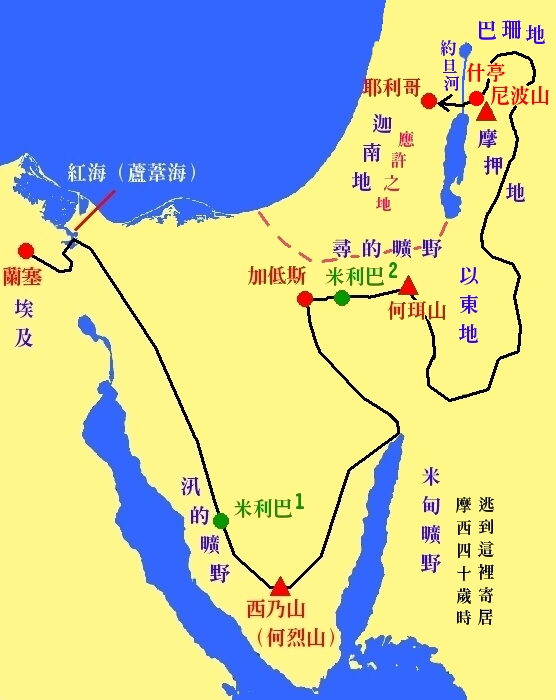
\includegraphics[width=0.8\textwidth]{AMoXiFigs/chuaiji/moses}
%\caption{以色列在曠野的經歷}
\label{fig:sub1}
\end{wrapfigure}
於是，摩西回到他岳父葉忒羅那裡，對他說：「求你容我回去見我在埃及的弟兄，看他們還在不在。」葉忒羅對摩西說：「你可以平平安安地去吧。」

\subsubsection{摩西回埃及的路上遇见神 4:19-26}

耶和華在米甸對摩西說：「你要回埃及去，因為尋索你命的人都死了。」摩西就帶著妻子和兩個兒子，叫他們騎上驢，回埃及地去。摩西手裡拿著神的杖。耶和華對摩西說：「你回到埃及的時候，要留意將我指示你的一切奇事行在法老面前。但我要使(任憑)他的心剛硬，他必不容百姓去。你要對法老說：『耶和華這樣說：以色列是我的兒子，我的長子。我對你說過容我的兒子去，好侍奉我，你還是不肯容他去。看哪，我要殺你的長子。』」摩西在路上住宿的地方，耶和華遇見他，想要殺他。西坡拉就拿一塊火石，割下他兒子的陽皮，丟在摩西腳前，說：「你真是我的血郎了！」 這樣，耶和華才放了他。西坡拉說：「你因割禮就是血郎了。」

\newpage
\subsubsection{亞倫迎接摩西 4:27-31}
耶和華對亞倫說：「你往曠野去迎接摩西。」他就去，在神的山遇見摩西，和他親嘴。 28 摩西將耶和華打發他所說的言語和囑咐他所行的神蹟都告訴了亞倫。 29 摩西、亞倫就去招聚以色列的眾長老。 30 亞倫將耶和華對摩西所說的一切話述說了一遍，又在百姓眼前行了那些神蹟。 31 百姓就信了。以色列人聽見耶和華眷顧他們，鑒察他們的困苦，就低頭下拜。


\section{以色列人出埃及 5-12}
\subsection{摩西亞倫見法老的第一回合 5:1-21}
\subsubsection{摩西亞倫初次見法老 5:1-5}
\begin{itemize} 
\itemsep-.35em 
\item 後來摩西、亞倫去對法老說：「耶和華以色列的神這樣說：『容我的百姓去，在曠野向我守節。』」法老說：「耶和華是誰，使我聽他的話，容以色列人去呢？我不認識耶和華，也不容以色列人去。」
\item 他們說：「希伯來人的神遇見了我們。求你容我們往曠野去，走三天的路程，祭祀耶和華我們的神，免得他用瘟疫、刀兵攻擊我們。」埃及王對他們說：「摩西，亞倫，你們為什麼叫百姓曠工呢？你們去擔你們的擔子吧！」又說：「看哪，這地的以色列人如今眾多，你們竟叫他們歇下擔子！」
\end{itemize}

\subsubsection{以色列人的官長受責罰 5:6-21}
\begin{itemize} 
\itemsep-.35em 
\item 當天，法老吩咐督工的和官長說：「你們不可照常把草給百姓做磚，叫他們自己去撿草。他們素常做磚的數目，你們仍舊向他們要，一點不可減少。因為他們是懶惰的，所以呼求說：『容我們去祭祀我們的神。』你們要把更重的工夫加在這些人身上，叫他們勞碌，不聽虛謊的言語。」
\item 以色列人的官長就來哀求法老說：「為什麼這樣待你的僕人？督工的不把草給僕人，並且對我們說：『做磚吧！』看哪，你僕人挨了打，其實是你百姓的錯。」 但法老說：「你們是懶惰的！你們是懶惰的！所以說：『容我們去祭祀耶和華。』現在你們去做工吧！草是不給你們的，磚卻要如數交納。」以色列人的官長聽說「你們每天做磚的工作一點不可減少」，就知道是遭遇禍患了。
\item 他們離了法老出來，正遇見摩西、亞倫站在對面，就向他們說：「願耶和華鑒察你們，施行判斷！因你們使我們在法老和他臣僕面前有了臭名，把刀遞在他們手中殺我們。」
\end{itemize}

\subsection{摩西亞倫見法老的第二回合 6:1-30}
\subsubsection{神向摩西亞倫確認應許 6:1-8}
\begin{itemize} 
\itemsep-.35em 
\item 耶和華對摩西說:現在你必看見我向法老所行的事,使他因我大能的手容以色列人去,且把他們趕出他的地
\item 神曉諭摩西說：「我是耶和華。我從前向亞伯拉罕、以撒、雅各顯現為全能的神，至於我名耶和華，他們未曾知道。我與他們堅定所立的約，要把他們寄居的迦南地賜給他們。我也聽見以色列人被埃及人苦待的哀聲，我也記念我的約。所以你要對以色列人說：我是耶和華，我要用伸出來的膀臂重重地刑罰埃及人，救贖你們脫離他們的重擔，不做他們的苦工。我要以你們為我的百姓，我也要做你們的神。你們要知道我是耶和華你們的神，是救你們脫離埃及人之重擔的。我起誓應許給亞伯拉罕、以撒、雅各的那地，我要把你們領進去，將那地賜給你們為業。我是耶和華。」
\end{itemize}

\subsubsection{人对神應許的反应 6:9-13}
\begin{itemize} 
\itemsep-.35em 
\item 摩西將這話告訴以色列人，只是他們因苦工愁煩，不肯聽他的話。
\item 耶和華曉諭摩西說： 「你進去對埃及王法老說，要容以色列人出他的地。」 
\item 摩西在耶和華面前說：「以色列人尚且不聽我的話，法老怎肯聽我這拙口笨舌的人呢？」\item 耶和華吩咐摩西、亞倫往以色列人和埃及王法老那裡去，把以色列人從埃及地領出來。
\end{itemize}

%\newpage
\subsubsection{摩西亞倫的家譜 6:14-25}
\begin{forest}
  for tree={
    child anchor=west,
    parent anchor=east,
    grow=east,
    draw,
    anchor=west,
    edge path={
      \noexpand\path[\forestoption{edge}]
        (.child anchor) -| +(-5pt,0) -- +(-5pt,0) |-
        (!u.parent anchor)\forestoption{edge label};
    },
  }
  [以色列
    [流便[哈諾] [法路] [希斯崙] [迦米]]
    [西緬[耶母利] [雅憫][阿轄][雅斤][瑣轄][掃羅（南女子的兒子）]]
    [利未（137歲）[約基別][革順[立尼][示每]] 
    					[哥轄（133歲）[暗蘭（妻子約基別）[亞倫（妻以利沙巴[拿答][亞比戶][以利亞撒[非尼哈]][以他瑪]][摩西][米利暗（姐姐）]
            ]
    									  [以斯哈[可拉[亞惜][以利加拿][亞比亞撒]][尼斐][細基利]]
    									  [希伯倫]
    									  [烏薛[米沙利][以利撒反][西提利]]] 
    					[米拉利[抹利][母示]]]                            
  ]
\end{forest}

\subsubsection{简介摩西亞倫 6:26-27}
\begin{itemize} 
\itemsep-.35em 
\item 亞倫的兒子以利亞撒娶了普鐵的一個女兒為妻，她給他生了非尼哈。這是利未人的家長，都按著他們的家
\item 耶和華說：「將以色列人按著他們的軍隊從埃及地領出來。」這是對那亞倫、摩西說的。對埃及王法老說要將以色列人從埃及領出來的，就是這摩西、亞倫。
\end{itemize}


\subsubsection{摩西亞倫受神命見法老 6:28-7:7}
\begin{itemize} 
\itemsep-.35em 
\item 當耶和華在埃及地對摩西說話的日子, 他向摩西說:我是耶和華，我對你說的一切話你都要告訴埃及王法老
\item 摩西在耶和華面前說：「看哪，我是拙口笨舌的人，法老怎肯聽我呢？」
\item 耶和華對摩西說：「我使你在法老面前代替神，你的哥哥亞倫是替你說話的。凡我所吩咐你的，你都要說。你的哥哥亞倫要對法老說，容以色列人出他的地。我要使法老的心剛硬，也要在埃及地多行神蹟奇事。但法老必不聽你們，我要伸手重重地刑罰埃及，將我的軍隊以色列民從埃及地領出來。我伸手攻擊埃及，將以色列人從他們中間領出來的時候，埃及人就要知道我是耶和華。」
\item 摩西、亞倫這樣行，耶和華怎樣吩咐他們，他們就照樣行了。摩西、亞倫與法老說話的時候，摩西八十歲，亞倫八十三歲
\end{itemize}

\subsubsection{杖變蛇為證 7:8-13}
\begin{itemize} 
\itemsep-.35em 
\item 耶和華曉諭摩西、亞倫說：「法老若對你們說：『你們行件奇事吧』，你就吩咐亞倫說：『把杖丟在法老面前，使杖變做蛇。』」
\item 摩西、亞倫進去見法老，就照耶和華所吩咐的行。亞倫把杖丟在法老和臣僕面前，杖就變做蛇。於是法老召了博士和術士來，他們是埃及行法術的，也用邪術照樣而行。他們各人丟下自己的杖，杖就變做蛇，但\underline{亞倫的杖吞了他們的杖}。
\item 法老心裡剛硬，不肯聽從摩西、亞倫，正如耶和華所說的。
\end{itemize}

\subsection{十災 6:28-12:36}



\subsubsection{水變血之災 7:14-25}
\begin{itemize} 
\itemsep-.35em 
\item 耶和華對摩西說：法老心裡固執，不肯容百姓去。明日早晨，他出來往水邊去，你要往河邊迎接他，手裡要拿著那變過蛇的杖
\begin{itemize} 
\itemsep-.35em 
\item 對他(法老)說：『耶和華希伯來人的神打發我來見你，說：「容我的百姓去，好在曠野侍奉我」，到如今你還是不聽。耶和華這樣說：我要用我手裡的杖擊打河中的水，水就變做血，因此你必知道我是耶和華。河裡的魚必死，河也要腥臭，埃及人就要厭惡吃這河裡的水。』
\item 耶和華曉諭摩西說：「你對亞倫說：『把你的杖伸在埃及所有的水以上，就是在他們的江、河、池、塘以上，叫水都變做血。在埃及遍地，無論在木器中、石器中，都必有血。』」
\end{itemize}
\item 摩西、亞倫就照耶和華所吩咐的行。亞倫在法老和臣僕眼前舉杖擊打河裡的水，河裡的水都變做血了。河裡的魚死了，河也腥臭了，埃及人就不能吃這河裡的水。埃及遍地都有了血。 
\item 埃及行法術的，也用邪術照樣而行。法老心裡剛硬，不肯聽摩西、亞倫，正如耶和華所說的。法老轉身進宮，也不把這事放在心上。埃及人都在河的兩邊挖地，要得水喝，因為他們不能喝這河裡的水。耶和華擊打河以後滿了七天。
\end{itemize}

\subsubsection{蛙災 8:1-15}
耶和華吩咐摩西說：「你進去見法老，對他說：『耶和華這樣說：容我的百姓去，好侍奉我。 2 你若不肯容他們去，我必使青蛙糟蹋你的四境。 3 河裡要滋生青蛙，這青蛙要上來進你的宮殿和你的臥房，上你的床榻，進你臣僕的房屋，上你百姓的身上，進你的爐灶和你的摶麵盆， 4 又要上你和你百姓並你眾臣僕的身上。』」

耶和華曉諭摩西說：「你對亞倫說：『把你的杖伸在江、河、池以上，使青蛙到埃及地上來。』」 6 亞倫便伸杖在埃及的諸水以上，青蛙就上來，遮滿了埃及地。 7 行法術的也用他們的邪術照樣而行，叫青蛙上了埃及地。

8 法老召了摩西、亞倫來，說：「請你們求耶和華，使這青蛙離開我和我的民，我就容百姓去祭祀耶和華。」 9 摩西對法老說：「任憑你吧！我要何時為你和你的臣僕並你的百姓祈求，除滅青蛙離開你和你的宮殿，只留在河裡呢？」 10 他說：「明天。」摩西說：「可以照你的話吧！好叫你知道沒有像耶和華我們神的。 11 青蛙要離開你和你的宮殿，並你的臣僕與你的百姓，只留在河裡。」 12 於是摩西、亞倫離開法老出去。摩西為擾害法老的青蛙呼求耶和華。 13 耶和華就照摩西的話行。凡在房裡、院中、田間的青蛙都死了。 14 眾人把青蛙聚攏成堆，遍地就都腥臭。 15 但法老見災禍鬆緩，就\textcolor{red}{硬著心}，不肯聽他們，正如耶和華所說的。


\subsubsection{蝨災 8:16-19}
耶和華吩咐摩西說：「你對亞倫說：『伸出你的杖擊打地上的塵土，使塵土在埃及遍地變做蝨子(虼蚤)。』」 17 他們就這樣行。亞倫伸杖擊打地上的塵土，就在人身上和牲畜身上有了蝨子，埃及遍地的塵土都變成蝨子了。 18 行法術的也用邪術要生出蝨子來，卻是不能。於是在人身上和牲畜身上都有了蝨子。

\subsubsection{蠅災 8:20-32}
耶和華對摩西說：「你清早起來，法老來到水邊，你站在他面前，對他說：『耶和華這樣說：容我的百姓去，好侍奉我。你若不容我的百姓去，我要叫成群的蒼蠅到你和你臣僕並你百姓的身上，進你的房屋，並且埃及人的房屋和他們所住的地都要滿了成群的蒼蠅。當那日，我必\textcolor{red}{分別}我百姓所住的歌珊地，使那裡沒有成群的蒼蠅，好叫你知道我是天下的耶和華。我要將我的百姓和你的百姓\textcolor{red}{分別}出來。明天必有這神蹟。』」耶和華就這樣行。蒼蠅成了大群，進入法老的宮殿和他臣僕的房屋，埃及遍地就因這成群的蒼蠅敗壞了。

法老召了摩西、亞倫來，說：「你們去，在這地祭祀你們的神吧！」摩西說：「這樣行本不相宜，因為我們要把埃及人所厭惡的祭祀耶和華我們的神。若把埃及人所厭惡的在他們眼前獻為祭，他們豈不拿石頭打死我們嗎？我們要往曠野去，走三天的路程，照著耶和華我們神所要吩咐我們的祭祀他。」法老說：「我容你們去，在曠野祭祀耶和華你們的神，只是不要走得很遠。求你們為我祈禱。」摩西說：「我要出去求耶和華，使成群的蒼蠅明天離開法老和法老的臣僕並法老的百姓，法老卻不可再行詭詐，不容百姓去祭祀耶和華。」 

於是摩西離開法老去求耶和華。 耶和華就照摩西的話行，叫成群的蒼蠅離開法老和他的臣僕並他的百姓，一個也沒有留下。這一次法老又\textcolor{red}{硬著心}，不容百姓去。


\subsubsection{畜疫之災 9:1-7}
耶和華吩咐摩西說：「你進去見法老，對他說：『耶和華希伯來人的神這樣說：容我的百姓去，好侍奉我。 2 你若不肯容他們去，仍舊強留他們， 3 耶和華的手加在你田間的牲畜上，就是在馬、驢、駱駝、牛群、羊群上，必有重重的瘟疫。 4 耶和華要\textcolor{red}{分別}以色列的牲畜和埃及的牲畜，凡屬以色列人的，一樣都不死。』」 5 耶和華就定了時候，說：「明天耶和華必在此地行這事。」 6 第二天，耶和華就行這事。埃及的牲畜幾乎都死了，只是以色列人的牲畜一個都沒有死。 7 法老打發人去看，誰知以色列人的牲畜連一個都沒有死。法老的心卻是\textcolor{red}{固執}，不容百姓去。

\subsubsection{人和牲畜身上起泡的瘡災 9:8-21}
耶和華吩咐摩西、亞倫說：「你們取幾捧爐灰，摩西要在法老面前向天揚起來。 9 這灰要在埃及全地變做塵土，在人身上和牲畜身上成了起泡的瘡。」 10 摩西、亞倫取了爐灰，站在法老面前。摩西向天揚起來，就在人身上和牲畜身上成了起泡的瘡。 11 行法術的在摩西面前站立不住，因為在他們身上和一切埃及人身上都有這瘡。 12 耶和華使法老的\textcolor{red}{心剛硬}，不聽他們，正如耶和華對摩西所說的。

13 耶和華對摩西說：「你清早起來，站在法老面前，對他說：『耶和華希伯來人的神這樣說：容我的百姓去，好侍奉我。 14 因為這一次我要叫一切的災殃臨到你和你臣僕並你百姓的身上，叫你知道在普天下沒有像我的。 15 我若伸手用瘟疫攻擊你和你的百姓，你早就從地上除滅了。 16 其實，我叫你存立，是特要向你顯我的大能，並要使我的名傳遍天下。 17 你還向我的百姓自高，不容他們去嗎？ 18 到明天約在這時候，我必叫重大的冰雹降下，自從埃及開國以來，沒有這樣的冰雹。 19 現在你要打發人把你的牲畜和你田間一切所有的催進來，凡在田間不收回家的，無論是人是牲畜，冰雹必降在他們身上，他們就必死。』」 20 法老的臣僕中，懼怕耶和華這話的，便叫他的奴僕和牲畜跑進家來。 21 但那不把耶和華這話放在心上的，就將他的奴僕和牲畜留在田裡。


\subsubsection{雹災 9:22-35}
耶和華對摩西說：「你向天伸杖，使埃及遍地的人身上和牲畜身上，並田間各樣菜蔬上，都有冰雹。」 23 摩西向天伸杖，耶和華就打雷下雹，有火閃到地上，耶和華下雹在埃及地上。 24 那時，雹與火摻雜，甚是厲害，自從埃及成國以來，遍地沒有這樣的。 25 在埃及遍地，雹擊打了田間所有的人和牲畜，並一切的菜蔬，又打壞田間一切的樹木。 26 唯獨以色列人所住的歌珊地沒有冰雹。
法老打發人召摩西、亞倫來，對他們說：「這一次我犯了罪了。耶和華是公義的，我和我的百姓是邪惡的。 28 這雷轟和冰雹已經夠了。請你們求耶和華，我就容你們去，不再留住你們。」 29 摩西對他說：「我一出城，就要向耶和華舉手禱告，雷必止住，也不再有冰雹，叫你知道全地都是屬耶和華的。 30 至於你和你的臣僕，我知道你們還是不懼怕耶和華神。」 31 那時，麻和大麥被雹擊打，因為大麥已經吐穗，麻也開了花。 32 只是小麥和粗麥沒有被擊打，因為還沒有長成。 33 摩西離了法老出城，向耶和華舉手禱告，雷和雹就止住，雨也不再澆在地上了。 34 法老見雨和雹與雷止住，就越發犯罪，他和他的臣僕都硬著心。 35 法老的\textcolor{red}{心剛硬}，不容以色列人去，正如耶和華藉著摩西所說的。

\subsubsection{蝗蟲之災 10:1-20}
 耶和華對摩西說：「你進去見法老。我使他和他臣僕的心剛硬，為要在他們中間顯我這些神蹟， 2 並要叫你將我向埃及人所做的事，和在他們中間所行的神蹟，傳於你兒子和你孫子的耳中，好叫你們知道我是耶和華。」 3 摩西、亞倫就進去見法老，對他說：「耶和華希伯來人的神這樣說：『你在我面前不肯自卑要到幾時呢？容我的百姓去，好侍奉我。 4 你若不肯容我的百姓去，明天我要使蝗蟲進入你的境內， 5 遮滿地面，甚至看不見地，並且吃那冰雹所剩的和田間所長的一切樹木。 6 你的宮殿和你眾臣僕的房屋，並一切埃及人的房屋，都要被蝗蟲占滿了。自從你祖宗和你祖宗的祖宗在世以來，直到今日，沒有見過這樣的災。』」摩西就轉身離開法老出去。 7 法老的臣僕對法老說：「這人為我們的網羅要到幾時呢？容這些人去侍奉耶和華他們的神吧！埃及已經敗壞了，你還不知道嗎？」 8 於是摩西、亞倫被召回來見法老，法老對他們說：「你們去侍奉耶和華你們的神，但那要去的是誰呢？」 9 摩西說：「我們要和我們老的少的、兒子女兒同去，且把羊群牛群一同帶去，因為我們務要向耶和華守節。」 10 法老對他們說：「我容你們和你們婦人孩子去的時候，耶和華與你們同在吧！你們要謹慎，因為有禍在你們眼前(你們存著惡意)。 11 不可都去，你們這壯年人去侍奉耶和華吧！因為這是你們所求的。」於是把他們從法老面前攆出去。
耶和華對摩西說：「你向埃及地伸杖，使蝗蟲到埃及地上來，吃地上一切的菜蔬，就是冰雹所剩的。」 13 摩西就向埃及地伸杖，那一晝一夜，耶和華使東風颳在埃及地上，到了早晨，東風把蝗蟲颳了來。 14 蝗蟲上來，落在埃及的四境，甚是厲害，以前沒有這樣的，以後也必沒有。 15 因為這蝗蟲遮滿地面，甚至地都黑暗了，又吃地上一切的菜蔬和冰雹所剩樹上的果子。埃及遍地，無論是樹木，是田間的菜蔬，連一點青的也沒有留下。 16 於是法老急忙召了摩西、亞倫來，說：「我得罪耶和華你們的神，又得罪了你們。 17 現在求你，只這一次，饒恕我的罪，求耶和華你們的神，使我脫離這一次的死亡。」 18 摩西就離開法老去求耶和華。 19 耶和華轉了極大的西風，把蝗蟲颳起，吹入紅海，在埃及的四境連一個也沒有留下。 20 但耶和華使法老的\textcolor{red}{心剛硬}，不容以色列人去。


\subsubsection{黑暗之災 10:21-29}
耶和華對摩西說：「你向天伸杖，使埃及地黑暗，這黑暗似乎摸得著。」 22 摩西向天伸杖，埃及遍地就烏黑了三天。 23 三天之久，人不能相見，誰也不敢起來離開本處，唯有以色列人家中都有亮光。 24 法老就召摩西來，說：「你們去侍奉耶和華，只是你們的羊群牛群要留下，你們的婦人孩子可以和你們同去。」 25 摩西說：「你總要把祭物和燔祭牲交給我們，使我們可以祭祀耶和華我們的神。 26 我們的牲畜也要帶去，連一蹄也不留下，因為我們要從其中取出來，侍奉耶和華我們的神。我們未到那裡，還不知道用什麼侍奉耶和華。」 27 但耶和華使法老的\textcolor{red}{心剛硬}，不肯容他們去。 28 法老對摩西說：「你離開我去吧！你要小心，不要再見我的面，因為你見我面的那日，你就必死！」 29 摩西說：「你說得好，我必不再見你的面了。」

\subsubsection{擊殺頭生的長子牲畜之災 11:1-12:30}
\subsubsubsection{以末次之災警告法老 11:1-10}
耶和華對摩西說：「我再使一樣的災殃臨到法老和埃及，然後他必容你們離開這地。他容你們去的時候，總要催逼你們都從這地出去。 2 你要傳於百姓的耳中，叫他們男女各人向鄰舍要金器銀器。」 3 耶和華叫百姓在埃及人眼前蒙恩，並且摩西在埃及地、法老臣僕和百姓的眼中看為極大。

4 摩西說：「耶和華這樣說：『約到半夜，我必出去巡行埃及遍地， 5 凡在埃及地，從坐寶座的法老直到磨子後的婢女所有的長子，以及一切頭生的牲畜，都必死。 6 埃及遍地必有大哀號，從前沒有這樣的，後來也必沒有。 7 至於以色列中，無論是人是牲畜，連狗也不敢向他們搖舌，好叫你們知道耶和華是將埃及人和以色列人分別出來。』 8 你這一切臣僕都要俯伏來見我，說：『求你和跟從你的百姓都出去』，然後我要出去。」於是，摩西氣憤憤地離開法老，出去了。

耶和華對摩西說：「法老必不聽你們，使我的奇事在埃及地多起來。」 10 摩西、亞倫在法老面前行了這一切奇事，耶和華使法老的心剛硬，不容以色列人出離他的地。

\subsubsubsection{定逾越節之禮 12:1-20}
\begin{itemize} 
\itemsep-.35em 
\item 逾越節 12:1-14
\begin{itemize} 
\itemsep-.35em 
\item 耶和華在埃及地曉諭摩西、亞倫說： 你們要以本月為正月，為一年之首。你們吩咐以色列全會眾說：\underline{本月初十日}，各人要按著父家取羊羔，一家一隻。若是一家的人太少，吃不了一隻羊羔，本人就要和他隔壁的鄰舍共取一隻。你們預備羊羔，要按著人數和飯量計算。要無殘疾、一歲的公羊羔，你們或從綿羊裡取，或從山羊裡取，都可以。 
\item 要留到\underline{本月十四日}，在黃昏的時候，以色列全會眾把羊羔宰了。各家要取點血，塗在吃羊羔的房屋左右的門框上和門楣上。當夜要吃羊羔的肉，用火烤了，與無酵餅和苦菜同吃。不可吃生的，斷不可吃水煮的，要帶著頭、腿、五臟，用火烤了吃。不可剩下一點留到早晨，若留到早晨，要用火燒了。你們吃羊羔當腰間束帶，腳上穿鞋，手中拿杖，趕緊地吃。這是耶和華的逾越節。 
\item 因為那夜我要巡行埃及地，把埃及地一切\underline{頭生的，無論是人是牲畜}，都擊殺了，又要敗壞埃及一切的\underline{神}。我是耶和華。這血要在你們所住的房屋上做記號，我一見這血，就越過你們去，我擊殺埃及地頭生的時候，災殃必不臨到你們身上滅你們。你們要記念這日，守為耶和華的節，作為你們世世代代永遠的定例。
\end{itemize}
\item 無酵節 12:15-20
\begin{itemize} 
\itemsep-.35em 
\item 你們要吃無酵餅\underline{七日}。頭一日要把酵從你們各家中除去，因為從頭一日起，到第七日為止，凡吃有酵之餅的，必從以色列中剪除。 
\item 頭一日你們當有聖會，第七日也當有聖會。這\underline{兩日}之內，除了預備各人所要吃的以外，無論何工都不可做。你們要守無酵節，因為我正當這日把你們的軍隊從埃及地領出來。所以你們要守這日，作為世世代代永遠的定例。 
\item 從\underline{正月十四日晚上，直到二十一日晚上}，你們要吃無酵餅。在你們各家中，七日之內不可有酵，因為凡吃有酵之物的，無論是寄居的是本地的，必從以色列的會中剪除。有酵的物，你們都不可吃，在你們一切住處要吃無酵餅。
\end{itemize}
\end{itemize}

\subsubsubsection{摩西吩咐百姓守逾越節之禮 12:21-28}
於是，摩西召了以色列的眾長老來，對他們說：「你們要按著家口取出羊羔，把這逾越節的羊羔宰了。 22 拿一把牛膝草，蘸盆裡的血，打在門楣上和左右的門框上。你們誰也不可出自己的房門，直到早晨。 23 因為耶和華要巡行擊殺埃及人，他看見血在門楣上和左右的門框上，就必越過那門，不容滅命的進你們的房屋，擊殺你們。 24 這例你們要守著，作為你們和你們子孫永遠的定例。 25 日後，你們到了耶和華按著所應許賜給你們的那地，就要守這禮。 26 你們的兒女問你們說：『行這禮是什麼意思？』 27 你們就說：『這是獻給耶和華逾越節的祭，當以色列人在埃及的時候，他擊殺埃及人，越過以色列人的房屋，救了我們各家。』」於是百姓低頭下拜。 28 耶和華怎樣吩咐摩西、亞倫，以色列人就怎樣行。

\subsubsubsection{耶和華擊殺埃及長子之災 12:29-30}
到了半夜，耶和華把埃及地所有的長子，就是從坐寶座的法老，直到被擄囚在監裡之人的長子，以及一切頭生的牲畜，盡都殺了。 30 法老和一切臣僕，並埃及眾人，夜間都起來了。在埃及有大哀號，無一家不死一個人的。

\subsection{以色列人出埃及 12:31-51}
\subsubsection{法老打發以色列人出離埃及 12:31-36}
夜間，法老召了摩西、亞倫來，說：「起來！連你們帶以色列人從我民中出去，依你們所說的去侍奉耶和華吧！ 32 也依你們所說的，連羊群牛群帶著走吧！並要為我祝福。」 33 埃及人催促百姓，打發他們快快出離那地，因為埃及人說：「我們都要死了。」 34 百姓就拿著沒有酵的生麵，把摶麵盆包在衣服中，扛在肩頭上。 35 以色列人照著摩西的話行，向埃及人要金器銀器和衣裳。 36 耶和華叫百姓在埃及人眼前蒙恩，以致埃及人給他們所要的。他們就把埃及人的財物奪去了。


\subsubsection{以色列人離開埃及 12:37-42}
以色列人從蘭塞起行，往疏割去，除了婦人孩子，步行的男人約有六十萬。 38 又有許多閒雜人，並有羊群牛群，和他們一同上去。 39 他們用埃及帶出來的生麵烤成無酵餅，這生麵原沒有發起，因為他們被催逼離開埃及，不能耽延，也沒有為自己預備什麼食物。 40 以色列人住在埃及共有四百三十年。 41 正滿了四百三十年的那一天，耶和華的軍隊都從埃及地出來了。 42 這夜是耶和華的夜，因耶和華領他們出了埃及地，所以當向耶和華謹守，是以色列眾人世世代代該謹守的。


\subsubsection{申明逾越節例 12:43-51}
耶和華對摩西、亞倫說：「逾越節的例是這樣：外邦人都不可吃這羊羔， 44 但各人用銀子買的奴僕，既受了割禮就可以吃。 45 寄居的和雇工人都不可吃。 46 應當在一個房子裡吃，不可把一點肉從房子裡帶到外頭去。羊羔的骨頭一根也不可折斷。 47 以色列全會眾都要守這禮。 48 若有外人寄居在你們中間，願向耶和華守逾越節，他所有的男子務要受割禮，然後才容他前來遵守，他也就像本地人一樣。但未受割禮的，都不可吃這羊羔。 49 本地人和寄居在你們中間的外人同歸一例。」 50 耶和華怎樣吩咐摩西、亞倫，以色列眾人就怎樣行了。 51 正當那日，耶和華將以色列人按著他們的\textcolor{red}{軍隊}，從埃及地領出來。


\section{以色列在曠野的經歷 13-18}
\sffamily\begin{tikzpicture}
  % Place all element in a matrix of nodes, called m
  % By default all nodes are rectangles with round corners
  % but some special sytles are defined also
  \matrix (m) [matrix of nodes, 
    column sep=5mm,
    row sep=1cm,
    nodes={draw, % General options for all nodes
      line width=1pt,
      anchor=center, 
      text centered,
      rounded corners,
      minimum width=1.5cm, minimum height=8mm
    }, 
    % Define styles for some special nodes
    right iso/.style={isosceles triangle,scale=0.5,sharp corners, anchor=center, xshift=-4mm},
    left iso/.style={right iso, rotate=180, xshift=-8mm},
    txt/.style={text width=1.5cm,anchor=center},
    ellip/.style={ellipse,scale=0.5},
    empty/.style={draw=none}
    ]   
  {
  % Second row of symbols
  % m-1-1
    蘭塞 
  & % m-1-2
    疏割
  & % m-1-3
    以倘   
   & % m-1-4
    比哈希錄  
   & % m-1-5
    |[draw=orange!80!white, ultra thick]| \textbf{密奪}   
   & % m-1-6
    |[coordinate, xshift=-1cm]|  
  \\  
  % Third row of symbols
    % m-2-1  
   瑪撒（探米）或叫米利巴（爭鬧）
  & % m-2-2試探
    |[draw=orange!80!white, ultra thick]| \textbf{汛的曠野} 
  & % m-2-3    
    以琳 
  & % m-2-4  
        |[draw=orange!80!white, ultra thick]| \textbf{瑪拉}       
  & % m-2-5  
    書珥曠野  
  & % m-2-6  (no symbol here, only a point to draw the path)
    |[coordinate, xshift=-1cm]| 
  \\  
利非訂
  & % m-3-1試探
  |[draw=orange!80!white, ultra thick]| \textbf{西乃曠野} 
  & % m-3-1試探
     |[coordinate, xshift=-1cm]| 
      \\     
  };  % End of matrix

  % Now, connect all nodes in a chain.
  % The names of the nodes are automatically generated in the previous matrix. Since the
  % matrix was named ``m'', all nodes have the name m-row-column
  { [start chain,every on chain/.style={join}, every join/.style={line width=1pt}]
    %\chainin (m-1-1);
  	 \chainin (m-1-1);
    \chainin (m-1-2);
    \chainin (m-1-3); 
    \chainin (m-1-4); 
    \chainin (m-1-5); 
    \path (m-1-5) edge node [below] {\small{3天}} (m-2-5) ; 
    \chainin (m-2-5);     
    \chainin (m-2-4);
    \chainin (m-2-3); 
    \chainin (m-2-2);  
    \chainin (m-2-1);  
   \chainin (m-3-1); 
       \path (m-3-1) edge node [below] {\small{葉忒羅}} (m-3-2) ;  
     \chainin (m-3-2);             
    };

                rotate=-90, minimum height=7mm, minimum width=1.3cm, 
                single arrow head extend=1.2mm, single arrow tip angle=120] {};
 
  % Define the style for the blue dotted boxes
  \tikzset{white dotted/.style={draw=white!50!white, line width=1pt,
                               dash pattern=on 1pt off 4pt on 6pt off 4pt,
                                inner sep=4mm, rectangle, rounded corners}};

  % Finally the blue dotted boxes are drawn as nodes fitted to other nodes
 % \node (first dotted box) [blue dotted, 
  %                          fit = (MOD text) (m-2-1) (m-2-4)] {};
  \node (second dotted box) [white dotted,
                            fit = (m-3-2)] {};
  \node at (second dotted box.south) [above, inner sep=1.mm] { \small{頒布律法，建會幕}};
  
  \node (second dotted box) [white dotted,
                            fit = (m-2-1)] {};
  \node at (second dotted box.south) [above, inner sep=1.mm] { \small{摩西擊打磐石}};

   \node (second dotted box) [white dotted,
                            fit = (m-3-1)] {};
  \node at (second dotted box.south) [above, inner sep=1.mm] { \small{與亞瑪力爭戰}};
 
  \node (second dotted box) [white dotted,
                            fit = (m-2-4)] {};
  \node at (second dotted box.south) [above, inner sep=1.mm] { \small{苦水變甜}};

  \node (second dotted box) [white dotted,
                            fit = (m-2-2)] {};
  \node at (second dotted box.south) [above, inner sep=1.mm] { \small{降鵪鶉和嗎哪}};


  % Define the style for the blue dotted boxes
  \tikzset{blue dotted/.style={draw=blue!50!white, line width=1pt,
                               dash pattern=on 1pt off 4pt on 6pt off 4pt,
                                inner sep=4mm, rectangle, rounded corners}};

  % Finally the blue dotted boxes are drawn as nodes fitted to other nodes
 % \node (first dotted box) [blue dotted, 
  %                          fit = (MOD text) (m-2-1) (m-2-4)] {};
  \node (second dotted box) [blue dotted,
                            fit = (m-1-1) (m-1-2) (m-1-3) (m-1-4) (m-1-5)] {};

  % Since these boxes are nodes, it is easy to put text above or below them                          
  %\node at (first dotted box.north) [above, inner sep=3mm] {\textbf{Transmitter}};
  %\node at (second dotted box.south) [below, inner sep=3mm] { \tiny{過紅海前}};
  \node at (second dotted box.south) [above, inner sep=1.mm] { \small{過紅海前}};

\end{tikzpicture}  

\begin{figure}%{.5\linewidth}
\centering
\includegraphics[width=5in]{AMoXiFigs/chuaiji/Exodus}
%\caption{以色列在曠野的經歷}
\label{fig:sub1}
\end{figure}

\begin{figure}%{.5\linewidth}
\centering
\includegraphics[width=6in]{AMoXiFigs/chuaiji/fig3}
%\caption{以色列在曠野的經歷}
\label{fig:sub1}
\end{figure}

\begin{figure}%{.5\linewidth}
\centering
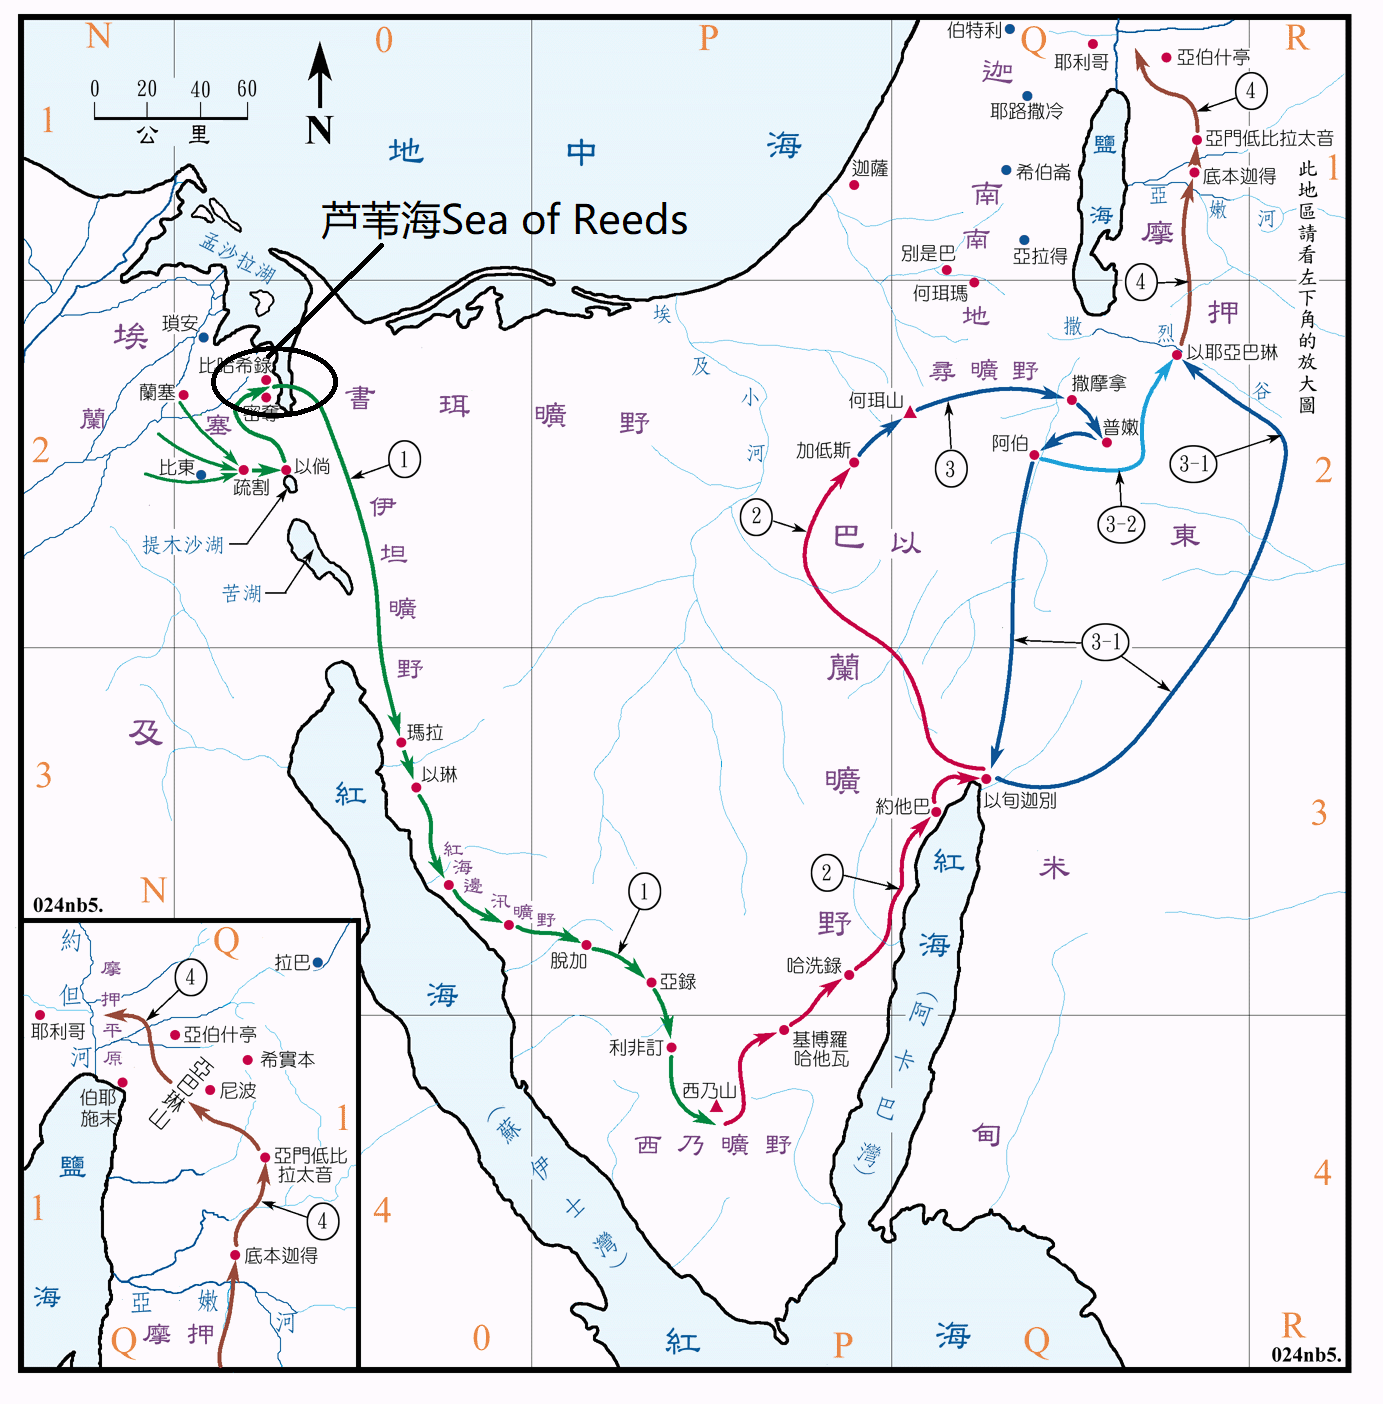
\includegraphics[width=6in]{AMoXiFigs/chuaiji/RedSee1}
%\caption{以色列在曠野的經歷}
\label{fig:sub1}
\end{figure}

\subsection{以色列人摆脱埃及軍隊 13:1-15:21}
\subsubsection{分別頭生 13:1-2(11-16)}
耶和華曉諭摩西說： 2 「以色列中凡頭生的，無論是人是牲畜，都是我的，要分別為聖歸我。」


\subsubsection{亞筆月向耶和華守無酵節七日 13:3-10}
摩西對百姓說：「你們要記念從埃及為奴之家出來的這日，因為耶和華用大能的手將你們從這地方領出來。有酵的餅都不可吃。 4 亞筆月間的這日是你們出來的日子。 5 將來耶和華領你進迦南人、赫人、亞摩利人、希未人、耶布斯人之地，就是他向你的祖宗起誓應許給你那流奶與蜜之地，那時你要在這月間守這禮。 6 你要吃無酵餅七日，到第七日要向耶和華守節。 7 這七日之久，要吃無酵餅，在你四境之內不可見有酵的餅，也不可見發酵的物。 8 當那日，你要告訴你的兒子說：『這是因耶和華在我出埃及的時候為我所行的事。』 9 這要在你手上做記號，在你額上做紀念，使耶和華的律法常在你口中，因為耶和華曾用大能的手將你從埃及領出來。 10 所以你每年要按著日期守這例。

\subsubsection{分別頭生公畜男婴 13:11-16}
將來，耶和華照他向你和你祖宗所起的誓將你領進迦南人之地，把這地賜給你， 12 那時你要將一切頭生的，並牲畜中頭生的，歸給耶和華，公的都要屬耶和華。 13 凡頭生的驢，你要用羊羔代贖，若不代贖，就要打折牠的頸項。凡你兒子中頭生的都要贖出來。 14 日後，你的兒子問你說：『這是什麼意思？』你就說：『耶和華用大能的手將我們從埃及為奴之家領出來。 15 那時法老幾乎不容我們去，耶和華就把埃及地所有頭生的，無論是人是牲畜，都殺了。因此，我把一切頭生的公牲畜獻給耶和華為祭，但將頭生的兒子都贖出來。 16 這要在你手上做記號，在你額上做經文，因為耶和華用大能的手將我們從埃及領出來。』」



\subsubsection{帶約瑟的骸骨繞道紅海曠野，日間雲柱和夜間火柱 13:17-22 }
17 法老容百姓去的時候，非利士地的道路雖近，神卻不領他們從那裡走，因為神說：「恐怕百姓遇見打仗後悔，就回埃及去。」 18 所以神領百姓繞道而行，走紅海曠野的路。以色列人出埃及地，都帶著兵器上去。 19 摩西把約瑟的骸骨一同帶去，因為約瑟曾叫以色列人嚴嚴地起誓，對他們說：「神必眷顧你們，你們要把我的骸骨從這裡一同帶上去。」 20 他們從疏割起行，在曠野邊的以倘安營。 21 日間耶和華在雲柱中領他們的路，夜間在火柱中光照他們，使他們日夜都可以行走。 22 日間雲柱，夜間火柱，總不離開百姓的面前。

%\vspace*{-\baselineskip}
\subsubsection{法老追襲以色列人 14:1-9}
耶和華曉諭摩西說： 2 「你吩咐以色列人轉回，安營在比哈希錄前、密奪和海的中間，對著巴力洗分，靠近海邊安營。 3 法老必說：『以色列人在地中繞迷了，曠野把他們困住了。』 4 我要使法老的心剛硬，他要追趕他們，我便在法老和他全軍身上得榮耀，埃及人就知道我是耶和華。」於是以色列人這樣行了。 5 有人告訴埃及王說：「百姓逃跑！」法老和他的臣僕就向百姓變心，說：「我們容以色列人去，不再服侍我們，這做的是什麼事呢？」 6 法老就預備他的車輛，帶領軍兵同去， 7 並帶著六百輛特選的車和埃及所有的車，每輛都有車兵長。 8 耶和華使埃及王法老的心剛硬，他就追趕以色列人，因為以色列人是昂然無懼地出埃及。 9 埃及人追趕他們，法老一切的馬匹、車輛、馬兵與軍兵就在海邊上，靠近比哈希錄，對著巴力洗分，在他們安營的地方追上了。

\begin{itemize} 
\itemsep-.35em 
\item 耶和華曉諭摩西說：「你\underline{吩咐以色列人轉回}，安營在比哈希錄前、密奪和海的中間，對著巴力洗分，靠近海邊安營。法老必說：『以色列人在地中繞迷了，曠野把他們困住了。』我要使法老的心剛硬，他要追趕他們，我便\underline{在法老和他全軍身上得榮耀，埃及人就知道我是耶和華}。」
\item 於是以色列人這樣行了。有人告訴埃及王說：「百姓逃跑！」法老和他的臣僕就向百姓變心，說：「我們容以色列人去，不再服侍我們，這做的是什麼事呢？」法老就預備他的車輛，帶領軍兵同去，並帶著六百輛特選的車和埃及所有的車，每輛都有車兵長。
\item 耶和華使埃及王法老的心剛硬，他就追趕以色列人，因為以色列人是昂然無懼地出埃及。埃及人追趕他們，法老一切的馬匹、車輛、馬兵與軍兵就在海邊上，靠近比哈希錄，對著巴力洗分，在他們安營的地方追上了。
\end{itemize}

\subsubsection{以色列人懼怕 14:10-14}
法老臨近的時候，以色列人舉目看見埃及人趕來，就甚懼怕，向耶和華哀求。 11 他們對摩西說：「難道在埃及沒有墳地，你把我們帶來死在曠野嗎？你為什麼這樣待我們，將我們從埃及領出來呢？ 12 我們在埃及豈沒有對你說過，不要攪擾我們，容我們服侍埃及人嗎？因為服侍埃及人比死在曠野還好。」 13 摩西對百姓說：「不要懼怕，只管站住，看耶和華今天向你們所要施行的救恩。因為你們今天所看見的埃及人，必永遠不再看見了。 14 耶和華必為你們爭戰，你們只管靜默，不要作聲。」

\begin{itemize} 
\itemsep-.35em 
\item 法老臨近的時候，以色列人舉目看見埃及人趕來，就甚懼怕，向耶和華哀求。他們對摩西說：「難道在埃及沒有墳地，你把我們帶來死在曠野嗎？你為什麼這樣待我們，將我們從埃及領出來呢？我們在埃及豈沒有對你說過，不要攪擾我們，容我們服侍埃及人嗎？因為服侍埃及人比死在曠野還好。」 
\item \underline{摩西對百姓說：「不要懼怕}，只管站住，看耶和華今天向你們所要施行的救恩。因為你們今天所看見的埃及人，必永遠不再看見了。耶和華必為你們爭戰，你們只管靜默，不要作聲。」
\end{itemize}

\subsubsection{紅海邊的雲柱拦阻埃及人 14:15-20}
耶和華對摩西說：「你為什麼向我哀求呢？你吩咐以色列人往前走。 16 你舉手向海伸杖，把水分開，以色列人要下海中走乾地。 17 我要使埃及人的心剛硬，他們就跟著下去，我要在法老和他的全軍、車輛、馬兵上得榮耀。 18 我在法老和他的車輛、馬兵上得榮耀的時候，埃及人就知道我是耶和華了。」 19 在以色列營前行走神的使者，轉到他們後邊去，雲柱也從他們前邊轉到他們後邊立住。 20 在埃及營和以色列營中間有雲柱，一邊黑暗，一邊發光，終夜兩下不得相近。

\begin{itemize} 
\itemsep-.35em 
\item 耶和華對摩西說：「你為什麼向我哀求呢？你吩咐以色列人往前走。你舉手向海伸杖，把水分開，以色列人要下海中走乾地。我要使埃及人的心剛硬，他們就跟著下去，我要在法老和他的全軍、車輛、馬兵上得榮耀。我在法老和他的車輛、馬兵上得榮耀的時候，埃及人就知道我是耶和華了。」 
\item 在以色列營前行走神的使者，轉到他們後邊去，雲柱也從他們前邊轉到他們後邊立住。在埃及營和以色列營中間有雲柱，一邊黑暗，一邊發光，終夜兩下不得相近
\end{itemize}

\subsubsection{投埃及人於海 14:21-31}
摩西向海伸杖，耶和華便用大東風使海水一夜退去，水便分開，海就成了乾地。 22 以色列人下海中走乾地，水在他們的左右做了牆垣。 23 埃及人追趕他們，法老一切的馬匹、車輛和馬兵都跟著下到海中。 24 到了晨更的時候，耶和華從雲火柱中向埃及的軍兵觀看，使埃及的軍兵混亂了， 25 又使他們的車輪脫落，難以行走，以致埃及人說：「我們從以色列人面前逃跑吧！因耶和華為他們攻擊我們了。」

耶和華對摩西說：「你向海伸杖，叫水仍合在埃及人並他們的車輛、馬兵身上。」 27 摩西就向海伸杖，到了天一亮，海水仍舊復原。埃及人避水逃跑的時候，耶和華把他們推翻在海中， 28 水就回流，淹沒了車輛和馬兵。那些跟著以色列人下海法老的全軍，連一個也沒有剩下。 29 以色列人卻在海中走乾地，水在他們的左右做了牆垣。 30 當日，耶和華這樣拯救以色列人脫離埃及人的手，以色列人看見埃及人的死屍都在海邊了。 31 以色列人看見耶和華向埃及人所行的大事，就敬畏耶和華，又信服他和他的僕人摩西。

\begin{itemize} 
\itemsep-.35em 
\item 摩西向海伸杖，耶和華便用\underline{大東風使海水一夜退去，水便分開，海就成了乾地}。
\begin{itemize} 
\itemsep-.35em 
\item 以色列人下海中走乾地，水在他們的左右做了牆垣。 
\item 埃及人追趕他們，法老一切的馬匹、車輛和馬兵都跟著下到海中。
\item 到了晨更的時候，耶和華\underline{從雲火柱中向埃及的軍兵觀看}，使埃及的軍兵混亂了，又使他們的車輪脫落，難以行走，以致埃及人說：「我們從以色列人面前逃跑吧！因耶和華為他們攻擊我們了。」
\end{itemize}
\item 耶和華對摩西說：「你向海伸杖，叫水仍合在埃及人並他們的車輛、馬兵身上。」摩西就向海伸杖，到了天一亮，\underline{海水仍舊復原}。 
\begin{itemize} 
\itemsep-.35em 
\item 埃及人避水逃跑的時候，耶和華把他們推翻在海中，水就回流，淹沒了車輛和馬兵。那些跟著以色列人下海法老的全軍，連一個也沒有剩下。
\item 以色列人卻在海中走乾地，水在他們的左右做了牆垣。當日，耶和華這樣拯救以色列人脫離埃及人的手,以色列人看見埃及人的死屍都在海邊了。以色列人看見耶和華向埃及人所行的大事，就敬畏耶和華，又信服他和他的僕人摩西。
\end{itemize}
\end{itemize}

\subsubsection{摩西歌頌耶和華 15:1-18}
\begin{itemize} 
\itemsep-.35em 
\item 那時，摩西和以色列人向耶和華\underline{唱歌}說：我要向耶和華歌唱,因他大大戰勝，將馬和騎馬的投在海中。耶和華是我的力量、我的詩歌，也成了我的拯救。這是我的神，我要讚美他；是我父親的神，我要尊崇他。耶和華是戰士，他的名是耶和華。\underline{法老}的車輛、軍兵，耶和華已拋在海中，他特選的軍長都沉於紅海。深水淹沒他們，他們如同石頭墜到深處。 耶和華啊，你的右手施展能力，顯出榮耀；耶和華啊，你的右手摔碎仇敵。你大發威嚴，推翻那些起來攻擊你的；你發出烈怒如火，燒滅他們像燒碎秸一樣。你發鼻中的氣，水便聚起成堆，大水直立如壘，海中的深水凝結。仇敵說：『我要追趕，我要追上；我要分擄物；我要在他們身上稱我的心願；我要拔出刀來，親手殺滅他們。』你叫風一吹，海就把他們淹沒，他們如鉛沉在大水之中。 
\item 耶和華啊，眾神之中誰能像你？誰能像你至聖至榮，可頌可畏，施行奇事？你伸出右手，地便吞滅他們。你憑慈愛領了你所贖的百姓，你憑能力引他們到了你的聖所。\underline{外邦人}聽見就發顫，疼痛抓住\underline{非利士}的居民。那時，\underline{以東}的族長驚惶，\underline{摩押}的英雄被戰兢抓住，\underline{迦南}的居民心都消化了，驚駭恐懼臨到他們。耶和華啊，因你膀臂的大能，他們如石頭寂然不動，等候你的百姓過去，等候你所贖的百姓過去。你要將他們領進去，栽於你產業的山上。耶和華啊，就是你為自己所造的住處；主啊，就是你手所建立的聖所。耶和華必做王，直到永永遠遠。」
\end{itemize}

\subsubsection{米利暗歌頌耶和華 15:19-21}
\begin{itemize} 
\itemsep-.35em
\item 法老的馬匹、車輛和馬兵下到海中，耶和華使海水回流淹沒他們，唯有以色列人在海中走乾地。 
\item 亞倫的姐姐女先知米利暗，手裡拿著鼓，眾婦女也跟她出去拿鼓跳舞。
\item 米利暗應聲說：「你們要歌頌耶和華，因他大大戰勝，將馬和騎馬的投在海中。」
\end{itemize}

\subsection{以色列人在曠野 15:22-18:27}
\subsubsection{在瑪拉因為水苦發怨言,樹使苦水變甜 15:22-26}
\begin{itemize} 
\itemsep-.35em
\item 摩西領以色列人從紅海往前行，到了書珥的曠野，在曠野走了三天，找不著水。到了瑪拉，不能喝那裡的水，因為水苦，所以那地名叫瑪拉。 
\item 百姓就向摩西發怨言，說：「我們喝什麼呢？」摩西呼求耶和華，耶和華指示他一棵樹。他把樹丟在水裡，水就變甜了。
\item 耶和華在那裡為他們定了律例、典章，在那裡試驗他們。又說：「你若留意聽耶和華你神的話，又行我眼中看為正的事，留心聽我的誡命，守我一切的律例，我就不將所加於埃及人的疾病加在你身上，因為我耶和華是醫治你的。」
\end{itemize}

\subsubsection{在以琳遇水泉十二 15:27}
\begin{itemize} 
\itemsep-.35em
\item 他們到了以琳，在那裡有十二股水泉，七十棵棕樹，
\item 他們就在那裡的水邊安營。
\end{itemize}

\subsubsection{汛的曠野因饥饿發怨言 16:1-3}
\begin{itemize} 
\itemsep-.35em
\item 以色列全會眾從以琳起行，在出埃及後第二個月十五日，到了以琳和西奈中間汛的曠野。
\item 以色列全會眾在曠野向摩西、亞倫發怨言，說：「巴不得我們早死在埃及地耶和華的手下，那時我們坐在肉鍋旁邊，吃得飽足。你們將我們領出來，到這曠野，是要叫這全會眾都餓死啊！」
\end{itemize}

\subsubsection{神应许賜鵪鶉和嗎哪 16:4-12}
\begin{itemize} 
\itemsep-.35em
\item 耶和華對摩西說：「我要將糧食從天降給你們。百姓可以出去，每天收每天的份，我好試驗他們遵不遵我的法度。到第六天，他們要把所收進來的預備好了，比每天所收的多一倍。」 摩西、亞倫對以色列眾人說：
\begin{itemize} 
\itemsep-.35em
\item 「到了晚上，你們要知道是耶和華將你們從埃及地領出來的。早晨，你們要看見耶和華的榮耀，因為耶和華聽見你們向他所發的怨言了。我們算什麼，你們竟向我們發怨言呢？」 
\item 摩西又說：「耶和華晚上必給你們肉吃，早晨必給你們食物得飽，因為你們向耶和華發的怨言，他都聽見了。我們算什麼？你們的怨言不是向我們發的，乃是向耶和華發的。」 
\item 摩西對亞倫說：「你告訴以色列全會眾說：『你們就近耶和華面前，因為他已經聽見你們的怨言了。』」 
\end{itemize}
\item 亞倫正對以色列全會眾說話的時候，他們向曠野觀看，不料，耶和華的榮光在雲中顯現。耶和華曉諭摩西說：「我已經聽見以色列人的怨言。你告訴他們說：『到黃昏的時候，你們要吃肉，早晨必有食物得飽，你們就知道我是耶和華你們的神。』」
\end{itemize}

\subsubsection{晚上賜鵪鶉，早晨降嗎哪 16:13-15}
\begin{itemize} 
\itemsep-.35em
\item 到了晚上，有\underline{鵪鶉}飛來，遮滿了營。
\item 早晨，在營四圍的地上有露水。露水上升之後，不料，野地面上有\underline{如白霜的小圓物}。
\item 以色列人看見不知道是什麼，就彼此對問說：「這是什麼呢？」摩西對他們說：「這就是耶和華給你們吃的食物
\end{itemize}

\subsubsection{收取嗎哪之例 16:16-30}
\begin{itemize} 
\itemsep-.35em
\item 耶和華所吩咐的是這樣：你們要按著各人的飯量，為帳篷裡的人按著人數收起來，各拿一俄梅珥。
\begin{itemize} 
\itemsep-.35em
\item 以色列人就這樣行，有多收的，有少收的。及至用俄梅珥量一量，多收的也沒有餘，少收的也沒有缺，各人\underline{按著自己的飯量收取}。 
\item 摩西對他們說：「所收的，\underline{不許什麼人留到早晨}。」然而他們不聽摩西的話，內中有留到早晨的，就生蟲變臭了。摩西便向他們發怒。
\end{itemize}
\item 他們每日早晨，按著各人的飯量收取，\underline{日頭一發熱就消化了}。 22 到\underline{第六天}，他們收了\underline{雙倍的食物}，每人兩俄梅珥。會眾的官長來告訴摩西， 23 摩西對他們說：「耶和華這樣說：『明天是聖安息日，是向耶和華守的聖安息日。你們要烤的就烤了，要煮的就煮了，所剩下的都留到早晨。』」
\item 他們就照摩西的吩咐留到早晨，也不臭，裡頭也沒有蟲子。 25 摩西說：「你們今天吃這個吧，因為今天是向耶和華守的安息日，你們在田野必找不著了。 26 六天可以收取，第七天乃是安息日，那一天必沒有了。」 
\item 第七天，百姓中有人出去收，什麼也找不著。耶和華對摩西說：「你們不肯守我的誡命和律法，要到幾時呢？ 29 你們看，耶和華既將安息日賜給你們，所以第六天他賜給你們兩天的食物，第七天各人要住在自己的地方，不許什麼人出去。」 於是百姓第七天安息了。
\end{itemize}

\subsubsection{嗎哪 16:31-36}
\begin{itemize} 
\itemsep-.35em
\item 這食物，以色列家叫嗎哪，樣子像芫荽子，顏色是白的，滋味如同攙蜜的薄餅。
\item 摩西說：「耶和華所吩咐的是這樣：要將一滿俄梅珥嗎哪留到世世代代，使後人可以看見我當日將你們領出埃及地，在曠野所給你們吃的食物。」摩西對亞倫說：「你拿一個罐子，盛一滿俄梅珥嗎哪，存在耶和華面前，要留到世世代代。」
\item 耶和華怎麼吩咐摩西，亞倫就怎麼行，把嗎哪放在法櫃前存留。以色列人吃嗎哪共四十年，直到進了有人居住之地，就是迦南的境界。（俄梅珥乃伊法十分之一。）
\end{itemize}

\subsubsection{米利巴摩西擊打磐石 17:1-7 (民數記20:1-13)}
\begin{itemize} 
\itemsep-.35em
\item 以色列全會眾都遵耶和華的吩咐，按著站口從汛的曠野往前行，在利非訂安營。
百姓沒有水喝，所以與摩西爭鬧，說：「給我們水喝吧！」摩西對他們說：「你們為什麼與我爭鬧，為什麼試探耶和華呢？」百姓在那裡甚渴，要喝水，就向摩西發怨言，說：「你為什麼將我們從埃及領出來，使我們和我們的兒女並牲畜都渴死呢？」 
\item 摩西就呼求耶和華說：「我向這百姓怎樣行呢？他們幾乎要拿石頭打死我。」耶和華對摩西說：「你手裡拿著你先前擊打河水的杖，帶領以色列的幾個長老，從百姓面前走過去。我必在何烈的磐石那裡，站在你面前。你要擊打磐石，從磐石裡必有水流出來，使百姓可以喝。」
\item 摩西就在以色列的長老眼前這樣行了。 
\begin{itemize} 
\itemsep-.35em
\item 他給那地方起名叫瑪撒 (試探)，
\item 又叫米利巴(爭鬧)，因以色列人爭鬧，又因他們試探耶和華，說：「耶和華是在我們中間不是？」
\end{itemize}
\end{itemize}

\subsubsection{與亞瑪力人爭戰 17:8-16 }
\begin{itemize} 
\itemsep-.35em
\item 那時，亞瑪力人來在利非訂，和以色列人爭戰。摩西對約書亞說：「你為我們選出人來，出去和亞瑪力人爭戰。明天我手裡要拿著神的杖，站在山頂上。」 
\begin{itemize} 
\itemsep-.35em
\item 於是約書亞照著摩西對他所說的話行，和亞瑪力人爭戰。
\item 摩西、亞倫與戶珥都上了山頂。摩西何時舉手，以色列人就得勝；何時垂手，亞瑪力人就得勝。但摩西的手發沉，他們就搬石頭來，放在他以下，他就坐在上面。亞倫與戶珥扶著他的手，一個在這邊，一個在那邊，他的手就穩住，直到日落的時候。
\item 約書亞用刀殺了亞瑪力王和他的百姓。 
\end{itemize}
\item 耶和華對摩西說：「我要將亞瑪力的名號從天下全然塗抹了，你要將這話寫在書上做紀念，又念給約書亞聽。」摩西築了一座壇，起名叫耶和華尼西 (耶和華是我旌旗)，又說：「耶和華已經起了誓，必世世代代和亞瑪力人爭戰。」
\end{itemize}

\subsubsection{摩西的岳父葉忒羅稱頌神 18:1-13 }
\begin{itemize} 
\itemsep-.35em
\item 摩西的岳父米甸祭司葉忒羅，聽見神為摩西和神的百姓以色列所行的一切事，就是耶和華將以色列從埃及領出來的事，便帶著摩西的妻子西坡拉，就是摩西從前打發回去的，又帶著西坡拉的兩個兒子，一個名叫革舜，因為摩西說：「我在外邦做了寄居的」，一個名叫以利以謝，因為他說：「我父親的神幫助了我，救我脫離法老的刀」——摩西的岳父葉忒羅帶著摩西的妻子和兩個兒子來到神的山，就是摩西在曠野安營的地方。
\item 他對摩西說：「我是你岳父葉忒羅，帶著你的妻子和兩個兒子來到你這裡。」摩西迎接他的岳父，向他下拜，與他親嘴，彼此問安，都進了帳篷。摩西將耶和華為以色列的緣故向法老和埃及人所行的一切事，以及路上所遭遇的一切艱難，並耶和華怎樣搭救他們，都述說於他岳父聽。
\item 葉忒羅因耶和華待以色列的一切好處，就是拯救他們脫離埃及人的手，便甚歡喜。
\begin{itemize} 
\itemsep-.35em
\item 葉忒羅說：「耶和華是應當稱頌的！他救了你們脫離埃及人和法老的手，將這百姓從埃及人的手下救出來。我現今在埃及人向這百姓發狂傲的事上得知，耶和華比萬神都大。」
\item 摩西的岳父葉忒羅把燔祭和平安祭獻給神。亞倫和以色列的眾長老都來了，與摩西的岳父在神面前吃飯
\end{itemize}
\end{itemize}

\subsubsection{葉忒羅獻策選立百姓官長 18:13-27 (申命記1:9-18)}
\begin{itemize} 
\itemsep-.35em
\item 第二天，摩西坐著審判百姓，百姓從早到晚都站在摩西的左右。
\begin{itemize} 
\itemsep-.35em
\item 摩西的岳父看見他向百姓所做的一切事，就說：「你向百姓做的是什麼事呢？你為什麼獨自坐著，眾百姓從早到晚都站在你的左右呢？」
\item 摩西對岳父說：「這是因百姓到我這裡來求問神。他們有事的時候就到我這裡來，我便在兩造之間施行審判，我又叫他們知道神的律例和法度。」 
\end{itemize}
\item 摩西的岳父說：「你這做的不好。你和這些百姓必都疲憊，因為這事太重，你獨自一人辦理不了。 現在你要聽我的話，我為你出個主意，願神與你同在。
\begin{itemize} 
\itemsep-.35em
\item 你要替百姓到神面前，將案件奏告神。又要將律例和法度教訓他們，指示他們當行的道、當做的事。
\item 並要從百姓中揀選有才能的人，就是敬畏神、誠實無妄、恨不義之財的人，派他們做千夫長、百夫長、五十夫長、十夫長，管理百姓。叫他們隨時審判百姓，大事都要呈到你這裡，小事他們自己可以審判
\item 這樣，你就輕省些，他們也可以同當此任。你若這樣行，神也這樣吩咐你，你就能受得住，這百姓也都平平安安歸回他們的住處。」 
\end{itemize}
\item 於是，摩西聽從他岳父的話，按著他所說的去行。摩西從以色列人中揀選了有才能的人，立他們為百姓的首領，做千夫長、百夫長、五十夫長、十夫長。他們隨時審判百姓，有難斷的案件就呈到摩西那裡，但各樣小事他們自己審判。此後，摩西讓他的岳父去，他就往本地去了
\end{itemize}

\section{西奈山得律法，建会幕和祭司体制 19-40}
\subsection{摩西一次上山得十誡 19:1-20:21}
\subsubsection{以色列人至西奈山 19:1-15 }
\begin{itemize} 
\itemsep-.35em
\item 以色列人出埃及地以後，滿了三個月的那一天，就來到西奈的曠野。他們離了利非訂，來到西奈的曠野，就在那裡的山下安營。摩西到神那裡，
\begin{table}[H]
\begin{threeparttable}
\begin{tabular}{@{}p{0.65\textwidth}*{4}{L{\dimexpr0.41\linewidth-10\tabcolsep\relax}}@{}}
\toprule
神 &  摩西 \\\hline
耶和華從山上呼喚他說：「你要這樣告訴雅各家，曉諭以色列人說：我向埃及人所行的事，你們都看見了；且看見我如鷹將你們背在翅膀上，帶來歸我。如今你們若實在聽從我的話，遵守我的約，就要在萬民中做屬我的子民，因為全地都是我的。你們要歸我做祭司的國度，為聖潔的國民。這些話你要告訴以色列人。」 &摩西去召了民間的長老來，將耶和華所吩咐他的話都在他們面前陳明。百姓都同聲回答說：「凡耶和華所說的，我們都要遵行。」摩西就將百姓的話回覆耶和華\tabularnewline\hline
耶和華對摩西說：「我要在密雲中臨到你那裡，叫百姓在我與你說話的時候可以聽見，也可以永遠信你了。」&於是，摩西將百姓的話奏告耶和華  \tabularnewline\hline
耶和華又對摩西說：「你往百姓那裡去，叫他們今天、明天自潔，又叫他們洗衣服。到第三天要預備好了，因為第三天耶和華要在眾百姓眼前降臨在西奈山上。你要在山的四圍給百姓定界限，說：『你們當謹慎，不可上山去，也不可摸山的邊界。凡摸這山的，必要治死他——不可用手摸他，必用石頭打死，或用箭射透。無論是人是牲畜，都不得活。到角聲拖長的時候，他們才可到山根來。』」&摩西下山往百姓那裡去，叫他們自潔，他們就洗衣服。他對百姓說：「到第三天要預備好了。不可親近女人。」 \tabularnewline
\hline
\bottomrule
\end{tabular}
\caption{百姓自潔豫備見神}
\end{threeparttable}
\end{table} 
\end{itemize}

\subsubsection{耶和華於火中降臨西奈山 19:16-25}
\begin{itemize} 
\itemsep-.35em
\item 到了第三天早晨
\begin{itemize} 
\itemsep-.35em
\item 在\underline{山上}有雷轟、閃電和密雲，並且角聲甚大
\item \underline{營中}的百姓盡都發顫。摩西率領百姓出營迎接神，都站在山下
\item 西奈\underline{全山}冒煙，因為耶和華在火中降於山上。山的煙氣上騰，如燒窯一般，遍山大大地震動。角聲漸漸地高而又高
\end{itemize}
\item 摩西就說話，神有聲音答應他。耶和華降臨在西奈山頂上，耶和華召摩西上山頂，摩西就上去。
\begin{table}[H]
\begin{threeparttable}
\begin{tabular}{@{}p{0.6\textwidth}*{4}{L{\dimexpr0.45\linewidth-10\tabcolsep\relax}}@{}}
\toprule
神 &  摩西 \\\hline
耶和華對摩西說：「你下去囑咐百姓，不可闖過來到我面前觀看，恐怕他們有多人死亡。又叫親近我的祭司自潔，恐怕我忽然出來擊殺他們。」&摩西對耶和華說：「百姓不能上西奈山，因為你已經囑咐我們說：『要在山的四圍定界限，叫山成聖。』」\tabularnewline\hline
耶和華對他說：「下去吧，你要和亞倫一同上來，只是祭司和百姓不可闖過來上到我面前，恐怕我忽然出來擊殺他們。」&於是摩西下到百姓那裡告訴他們。 \tabularnewline\hline
\hline
\bottomrule
\end{tabular}
\caption{耶和華於火中降臨西奈山}
\end{threeparttable}
\end{table} 
\end{itemize}


\subsubsection{頒布十誡 20:1-17 (申5:6-21)}
\begin{itemize} 
\itemsep-.35em
\item 对神的条例
\begin{itemize} 
\itemsep-.35em
\item 神吩咐這一切的話說：「我是耶和華你的神，曾將你從埃及地為奴之家領出來。除了我以外，你\underline{不可有別的神}
\item \underline{不可為自己雕刻偶像}，也不可做什麼形象彷彿上天、下地和地底下、水中的百物。不可跪拜那些像，也不可侍奉它，因為我耶和華你的神是忌邪的神。恨我的，我必追討他的罪，自父及子，直到三四代；愛我守我誡命的，我必向他們發慈愛，直到千代
\item \underline{不可妄稱耶和華你神的名}，因為妄稱耶和華名的，耶和華必不以他為無罪
\item \underline{當記念安息日}，守為聖日。六日要勞碌做你一切的工，但第七日是向耶和華你神當守的安息日。這一日你和你的兒女、僕婢、牲畜，並你城裡寄居的客旅，無論何工都不可做。因為六日之內，耶和華造天、地、海和其中的萬物，第七日便安息，所以耶和華賜福於安息日，定為聖日
\end{itemize}
\item 对人的条例
\begin{itemize} 
\itemsep-.35em
\item \underline{當}孝敬父母，使你的日子在耶和華你神所賜你的地上得以長久
\item \underline{不可}殺人
\item \underline{不可}姦淫
\item \underline{不可}偷盜
\item \underline{不可}作假見證陷害人
\item \underline{不可}貪戀人的房屋，也不可貪戀人的妻子、僕婢、牛驢並他一切所有的。
\end{itemize}
\end{itemize}


\subsubsection{百姓見神而懼怕 20:18-21 (申命記5:23-27)}
\begin{itemize} 
\itemsep-.35em
\item 眾百姓見雷轟、閃電、角聲、山上冒煙，就都發顫，遠遠地站立，對摩西說：「求你和我們說話，我們必聽；不要神和我們說話，恐怕我們死亡。」 
\item 摩西對百姓說：「不要懼怕，因為神降臨是要試驗你們，叫你們時常敬畏他，不致犯罪。」於是百姓遠遠地站立，摩西就挨近神所在的幽暗之中。
\end{itemize}


\subsection{摩西二次上山得律法 20:22-23:33}
\subsubsection{禁造神像和築（土、石）壇之條例 20:22-26}
\begin{itemize} 
\itemsep-.35em
\item 耶和華對摩西說：「你要向以色列人這樣說：你們自己看見我從天上和你們說話了。你們\underline{不可做什麼神}像與我相配，不可為自己做金銀的神像。
\item 你要為我\underline{築土壇}，在上面以牛羊獻為燔祭和平安祭。凡記下我名的地方，我必到那裡賜福給你。
 \item 你若為我\underline{築一座石壇}，不可用鑿成的石頭，因你在上頭一動家具，就把壇汙穢了。
\item 你上我的壇，\underline{不可用臺階}，免得露出你的下體來。
\end{itemize}


\subsubsection{對待奴僕之例 21:1-11 （申15:12-18/利25:39-55）}
\begin{itemize} 
\itemsep-.35em
\item 男僕：你在百姓面前所要立的典章是這樣：你若買希伯來人做奴僕
\begin{itemize} 
\itemsep-.35em
\item 他必服侍你六年，第七年他可以自由，白白地出去。
\begin{itemize} 
\itemsep-.35em
\item 他若孤身來，就可以孤身去；
\item 他若有妻，他的妻就可以同他出去。
\item 他主人若給他妻子，妻子給他生了兒子或女兒，妻子和兒女要歸主人，他要獨自出去。
\end{itemize}
\item 倘或奴僕明說：『我愛我的主人和我的妻子、兒女，不願意自由出去。』他的主人就要帶他到審判官（神）那裡，又要帶他到門前，靠近門框，用錐子穿他的耳朵，他就永遠服侍主人。
\end{itemize}
\item 女僕：人若賣女兒做婢女，婢女不可像男僕那樣出去。
\begin{itemize} 
\itemsep-.35em
\item 主人選定她歸自己，若不喜歡她，就要許她贖身；主人既然用詭詐待她，就沒有權柄賣給外邦人。
\item 主人若選定她給自己的兒子，就當待她如同女兒。若另娶一個，那女子的吃食、衣服並好合的事，仍不可減少。若不向她行這三樣，她就可以不用錢贖，白白地出去。
\end{itemize}
\end{itemize}

\subsubsection{人傷害人的赔偿條例 21:12-27}
\begin{itemize} 
\itemsep-.35em
\item 人若彼此相爭
\begin{itemize} 
\itemsep-.35em
\item 打人以致打死的，必要把他治死。人若不是埋伏著殺人，乃是神交在他手中，我就設下一個地方，他可以往那裡逃跑。人若任意用詭計殺了他的鄰舍，就是逃到我的壇那裡，也當捉去把他治死。
\item 人若彼此相爭，這個用石頭或是拳頭打那個，尚且不至於死，不過躺臥在床，若再能起來扶杖而出，那打他的可算無罪，但要將他耽誤的工夫用錢賠補，並要將他全然醫好。
\item 人若彼此爭鬥，傷害有孕的婦人，甚至墜胎，隨後卻無別害，那傷害她的總要按婦人的丈夫所要的，照審判官所斷的受罰。若有別害，就要以命償命，以眼還眼，以牙還牙，以手還手，以腳還腳，以烙還烙，以傷還傷，以打還打。
\end{itemize}
\item 拐帶人口，或是把人賣了，或是留在他手下，必要把他治死。
\item 人若与父母相爭
\begin{itemize} 
\itemsep-.35em
\item 打父母的，必要把他治死。
\item 咒罵父母的，必要把他治死。
\end{itemize}
\item 打死打壞奴僕
\begin{itemize} 
\itemsep-.35em
\item 人若用棍子打奴僕或婢女，立時死在他的手下，他必要受刑。若過一兩天才死，就可以不受刑，因為是用錢買的。
\item 人若打壞了他奴僕或是婢女的一隻眼，就要因他的眼放他去得以自由。若打掉了他奴僕或是婢女的一個牙，就要因他的牙放他去得以自由。
\end{itemize}
\end{itemize}

\subsubsection{人傷動物或動物傷人的條例 21:28-36}
\begin{itemize} 
\itemsep-.35em
\item 牛若觸死男人或是女人
\begin{itemize} 
\itemsep-.35em
\item 牛若觸了自由人
\begin{itemize} 
\itemsep-.35em
\item 總要用石頭打死那牛，卻不可吃牠的肉，牛的主人可算無罪。
\item 倘若那牛素來是觸人的，有人報告了牛主，他竟不把牛拴著，以致把男人或是女人觸死，就要用石頭打死那牛，牛主也必治死。
\item 若罰他贖命的價銀，他必照所罰的贖他的命。
\item 牛無論觸了人的兒子或是女兒，必照這例辦理。
\end{itemize}
\item 牛若觸了奴僕或是婢女，必將銀子三十舍客勒給他們的主人，也要用石頭把牛打死。
\end{itemize}
\item 人若敞著井口，或挖井不遮蓋，有牛或驢掉在裡頭，井主要拿錢賠還本主人，死牲畜要歸自己
\item 牛傷牛
\begin{itemize} 
\itemsep-.35em
\item 這人的牛若傷了那人的牛，以至於死，他們要賣了活牛，平分價值，也要平分死牛。 \item 人若知道這牛素來是觸人的，主人竟不把牛拴著，他必要以牛還牛，死牛要歸自己
\end{itemize}
\end{itemize}

\subsubsection{賠償的條例 22:1-17}
\begin{itemize} 
\itemsep-.35em
\item 牲畜造成的损失
\begin{itemize} 
\itemsep-.35em
\item 人若偷牛或羊，無論是宰了是賣了，他就要以五牛賠一牛，四羊賠一羊。
\item 人若遇見賊挖窟窿，把賊打了，以至於死，就不能為他有流血的罪。若太陽已經出來，就為他有流血的罪。
\item 賊若被拿，總要賠還。若他一無所有，就要被賣，頂他所偷的物。若他所偷的，或牛，或驢，或羊，仍在他手下存活，他就要加倍賠還。
\item 人若在田間或在葡萄園裡放牲畜，任憑牲畜上別人的田裡去吃，就必拿自己田間上好的和葡萄園上好的賠還。
\end{itemize}
\item 人为造成的损失
\begin{itemize} 
\itemsep-.35em
\item 若點火焚燒荊棘，以致將別人堆積的禾捆、站著的禾稼或是田園，都燒盡了，那點火的必要賠還。
\item 人若將銀錢或家具交付鄰舍看守，這物從那人的家被偷去，若把賊找到了，賊要加倍賠還。若找不到賊，那家主必就近審判官，要看看他拿了原主的物件沒有。兩個人的案件，無論是為什麼過犯，或是為牛，為驢，為羊，為衣裳，或是為什麼失掉之物，有一人說『這是我的』，兩造就要將案件稟告審判官，審判官定誰有罪，誰就要加倍賠還。
\item 人若將驢，或牛，或羊，或別的牲畜，交付鄰舍看守，牲畜或死，或受傷，或被趕去，無人看見，那看守的人要憑著耶和華起誓，手裡未曾拿鄰舍的物，本主就要罷休，看守的人不必賠還。牲畜若從看守的那裡被偷去，他就要賠還本主。若被野獸撕碎，看守的要帶來當做證據，所撕的不必賠還。
\item 人若向鄰舍借什麼，所借的或受傷，或死，本主沒有同在一處，借的人總要賠還。若本主同在一處，他就不必賠還。若是雇的，也不必賠還，本是為雇價來的。
\item 人若引誘沒有受聘的處女，與她行淫，他總要交出聘禮，娶她為妻。若女子的父親決不肯將女子給他，他就要按處女的聘禮，交出錢來。
\end{itemize}
\end{itemize}

\subsubsection{敬畏神和不可虧負弱者的條例 22:18-31}
\begin{itemize} 
\itemsep-.35em
\item 敬畏神的条例
\begin{itemize} 
\itemsep-.35em
\item 行邪術的女人，不可容她存活。
\item 凡與獸淫合的，總要把他治死。
\item 祭祀別神，不單單祭祀耶和華的，那人必要滅絕。
\item 不可毀謗神，也不可毀謗你百姓的官長。
\item 你要從你莊稼中的穀和酒榨中滴出來的酒拿來獻上，不可遲延。你要將頭生的兒子歸給我。 你牛羊頭生的，也要這樣，七天當跟著母，第八天要歸給我。
\item 你要在我面前為聖潔的人，因此，田間被野獸撕裂牲畜的肉，你們不可吃，要丟給狗吃
\end{itemize}
\item 不可虧負弱者
\begin{itemize} 
\itemsep-.35em
\item 不可虧負寄居的，也不可欺壓他，因為你們在埃及地也做過寄居的。
\item 不可苦待寡婦和孤兒。若是苦待他們一點，他們向我一哀求，我總要聽他們的哀聲，並要發烈怒，用刀殺你們，使你們的妻子為寡婦，兒女為孤兒。
\item 我民中有貧窮人與你同住，你若借錢給他，不可如放債的向他取利。你即或拿鄰舍的衣服做當頭，必在日落以先歸還他。因他只有這一件當蓋頭，是他蓋身的衣服，若是沒有，他拿什麼睡覺呢？他哀求我，我就應允，因為我是有恩惠的。
\end{itemize}
\end{itemize}


\subsubsection{行公义的条例 23:1-9}
\begin{itemize} 
\itemsep-.35em
\item 不可隨夥布散謠言，不可與惡人連手妄作見證。不可隨眾行惡，不可在爭訟的事上隨眾偏行，作見證屈枉正直。也不可在爭訟的事上偏護窮人。
\item 若遇見你仇敵的牛或驢失迷了路，總要牽回來交給他。若看見恨你人的驢壓臥在重馱之下，不可走開，務要和驢主一同抬開重馱。
\item 不可在窮人爭訟的事上屈枉正直。當遠離虛假的事。不可殺無辜和有義的人，因我必不以惡人為義。
\item 不可受賄賂，因為賄賂能叫明眼人變瞎了，又能顛倒義人的話。
\item 不可欺壓寄居的，因為你們在埃及地做過寄居的，知道寄居的心。
\end{itemize}

\subsubsection{安息年，安息日之例 23:10-13(31:12-18/34:21/35:1-3)}
\begin{itemize} 
\itemsep-.35em
\item 六年你要耕種田地，收藏土產，只是第七年要叫地歇息，不耕不種，使你民中的窮人有吃的，他們所剩下的，野獸可以吃。你的葡萄園和橄欖園也要照樣辦理。
\item 六日你要做工，第七日要安息，使牛、驢可以歇息，並使你婢女的兒子和寄居的都可以舒暢。 
\item 凡我對你們說的話，你們要謹守。別神的名，你不可提，也不可從你口中傳說。
\end{itemize}

\subsubsection{除酵節，收割節（七七節），收藏節 23:14-17 (34:18-24)}
\begin{itemize} 
\itemsep-.35em
\item 一年三次，你要向我守節
\begin{itemize} 
\itemsep-.35em
\item 你要守除酵節，照我所吩咐你的，在亞筆月內所定的日期，吃無酵餅七天。誰也不可空手朝見我，因為你是這月出了埃及。
\item 又要守收割節，所收的是你田間所種、勞碌得來初熟之物。
\item 並在年底收藏，要守收藏節
\end{itemize}
一切的男丁要一年三次朝見主耶和華。
\end{itemize}

\subsubsection{當獻初熟之物 23:18-19}
\begin{itemize} 
\itemsep-.35em
\item 不可將我祭牲的血和有酵的餅一同獻上
\item 也不可將我節上祭牲的脂油留到早晨
\item 地裡首先初熟之物要送到耶和華你神的殿
\item 不可用山羊羔母的奶煮山羊羔。
\end{itemize}

\subsubsection{復許導以色列民進迦南 23:20-23}
\begin{itemize} 
\itemsep-.35em
\item 看哪，我差遣使者在你前面，在路上保護你，領你到我所預備的地方去。他是奉我名來的，你們要在他面前謹慎，聽從他的話，不可惹（違背）他，因為他必不赦免你們的過犯。
\item 你若實在聽從他的話，照著我一切所說的去行，我就向你的仇敵做仇敵，向你的敵人做敵人。我的使者要在你前面行，領你到亞摩利人、赫人、比利洗人、迦南人、希未人、耶布斯人那裡去，我必將他們剪除。
\end{itemize}

\subsubsection{不可事奉迦南地人的神 23:21-33}
\begin{itemize} 
\itemsep-.35em
\item 你不可跪拜他們的神，不可侍奉他，也不可效法他們的行為，卻要把神像盡行拆毀，打碎他們的柱像。你們要侍奉耶和華你們的神
\begin{itemize} 
\itemsep-.35em
\item 他必賜福於你的糧與你的水，也必從你們中間除去疾病。你境內必沒有墜胎的、不生產的；我要使你滿了你年日的數目。
\item 凡你所到的地方，我要使那裡的眾民在你面前驚駭擾亂，又要使你一切仇敵轉背逃跑。我要打發黃蜂飛在你前面，把希未人、迦南人、赫人攆出去。我不在一年之內將他們從你面前攆出去，恐怕地成為荒涼，野地的獸多起來害你。我要漸漸地將他們從你面前攆出去，等到你的人數加多，承受那地為業。我要定你的境界，從紅海直到非利士海，又從曠野直到大河。我要將那地的居民交在你手中，你要將他們從你面前攆出去
\end{itemize}
\item 不可和他們並他們的神立約。他們不可住在你的地上，恐怕他們使你得罪我。你若侍奉他們的神，這必成為你的網羅。」
\end{itemize}


\subsection{摩西三次上山得建造会幕和祭司体系的启示 24-31}
\subsubsection{神召摩西及以色列的領袖上山見神 24:1-11}
\begin{itemize} 
\itemsep-.35em
\item 耶和華對摩西說：「你和亞倫、拿答、亞比戶，並以色列長老中的七十人，都要上到我這裡來，遠遠地下拜。唯獨你可以親近耶和華，他們卻不可親近，百姓也不可和你一同上來。」 
\item 摩西下山，將耶和華的命令、典章都述說於百姓聽，眾百姓齊聲說：「耶和華所吩咐的，我們都必遵行。」
\begin{itemize} 
\itemsep-.35em
\item 摩西將耶和華的命令都寫上。清早起來，在山下築一座壇，按以色列十二支派立十二根柱子， \item 又打發以色列人中的少年人去獻燔祭，又向耶和華獻牛為平安祭。摩西將血一半盛在盆中一半灑在壇上
\item 又將約書念給百姓聽，他們說：「耶和華所吩咐的，我們都必遵行。」 
\item 摩西將血灑在百姓身上，說：「你看，這是立約的血，是耶和華按這一切話與你們立約的憑據
\end{itemize}
\item 摩西、亞倫、拿答、亞比戶，並以色列長老中的七十人，都上了山。他們看見以色列的神，他腳下彷彿有平鋪的藍寶石，如同天色明淨。他的手不加害在以色列的尊者身上。他們觀看神，他們又吃又喝
\end{itemize}

\subsubsection{摩西三次上山見神 24:12-18}
\begin{itemize} 
\itemsep-.35em
\item 耶和華對摩西說:你上山到我這裡來住在這裡，我要將石版並我所寫的律法和誡命賜給你，使你可以教訓百姓 
\item 摩西和他的幫手約書亞起來，上了神的山。
\begin{itemize} 
\itemsep-.35em
\item 摩西對長老說：「你們在這裡等著，等到我們再回來。有亞倫、戶珥與你們同在，凡有爭訟的，都可以就近他們去。」 
\item 摩西上山，有雲彩把山遮蓋。耶和華的榮耀停於西奈山，雲彩遮蓋山六天，第七天他從雲中召摩西。耶和華的榮耀在山頂上，在以色列人眼前，形狀如烈火。摩西進入雲中上山，在山上四十晝夜。
\end{itemize}
\end{itemize}


\subsubsection{造聖所奉獻的物 25:1-9 （35:4-9）}
\begin{figure}%{.5\linewidth}
\centering
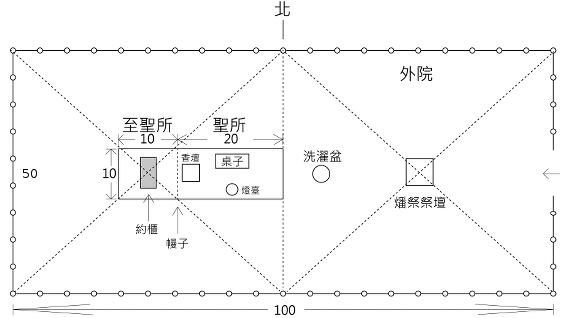
\includegraphics[width=5in]{AMoXiFigs/chuaiji/HuiMu}
%\caption{聖所}
\label{fig:sub1}
\end{figure}
\begin{figure}%{.5\linewidth}
\centering
%
\includegraphics{AMoXiFigs/HuiMuTu.gif}
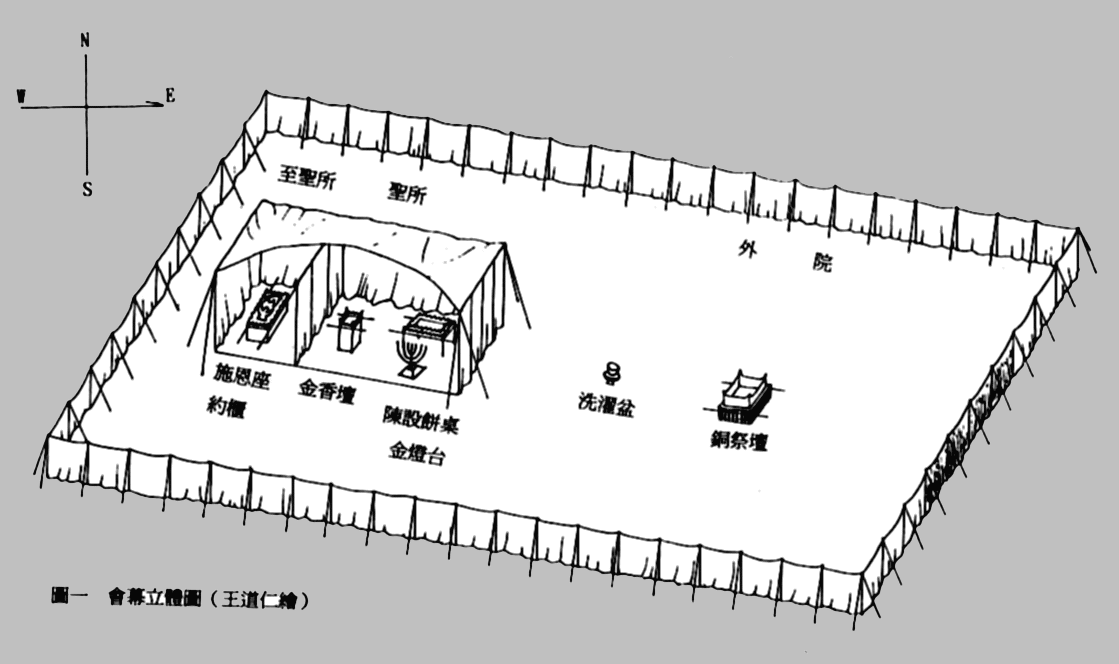
\includegraphics[width=5in]{AMoXiFigs/chuaiji/HuiMuTu}
%\caption{聖所}
\label{fig:sub1}
\end{figure}

\begin{itemize} 
\itemsep-.35em
\item 耶和華曉諭摩西說:你告訴以色列人當為我送禮物來，凡甘心樂意的你們就可以收下歸我。所要收的禮物是
\begin{table}[H]
\centering
\begin{tabular}{|c|c| }
\hline
\hline
材料 & 名稱  \\\hline
金屬 & 金、銀、銅    \\\hline
線類&藍色、紫色、朱紅色線、細麻、山羊毛  \\\hline
皮類&染紅的公羊皮、海狗皮 \\\hline
木類&　皂莢木 　\\\hline
油、香料&點燈的油並做膏油和香的香料　\\\hline
寶石&紅瑪瑙與別樣的寶石，可以鑲嵌在以弗得和胸牌上 \\\hline
\end{tabular}
\caption{奉獻的物}
\end{table}
\item 又當為我造聖所，使我可以住在他們中間。製造帳幕和其中的一切器具，都要照我所指示你的樣式
\end{itemize}

\subsubsection{造約櫃之法則 25:10-22 （37:1-9）}
\begin{itemize} 
\itemsep-.35em
\item 造約櫃之法則
\begin{table}[H]
\centering
\begin{tabular}{|c|l| }
\hline
\hline
部件 & 规格  \\\hline
約櫃 & 皂莢木，長2.5肘 X 寬1.5肘 X 高1.5肘，裡外包上精金、四圍鑲上金牙邊    \\\hline
金環&鑄四個金環安在櫃的四腳上、這邊兩環、那邊兩環。   \\\hline
抬杠&用皂莢木做兩根槓用金包裹。要把槓穿在櫃旁的環內以便抬櫃。這槓要常在櫃的環內，不可抽出來\\\hline
櫃裡&必將我所要賜給你的法版放在櫃裡　\\\hline
施恩座&要用精金做施恩（蔽罪）座，要將施恩座安在櫃的上邊，長2.5肘 X 寬1.5肘　\\\hline
基路伯&要用金子錘出兩個基路伯來，安在施恩座的兩頭。二基路伯要接連一塊。二基路伯要高張翅膀\\
&遮掩施恩座。基路伯要臉對臉，朝著施恩座。要將施恩座安在櫃的上邊  \\\hline
\end{tabular}
\caption{造約櫃之法則}
\end{table}
\item 我要在那裡與你相會，又要從法櫃施恩座上二基路伯中間，和你說我所要吩咐你傳給以色列人的一切事
\end{itemize}

\subsubsection{造陳設餅的桌子及器皿 25:23-30  （37:10-16）}
\begin{table}[H]
\centering
\begin{tabular}{|c|l| }
\hline
\hline
部件 & 规格   \\\hline
桌子 &要用皂莢木做一張桌子，長2肘 X 寬1肘 X 高1肘，包上精金、四圍鑲上金牙邊    \\\hline
橫梁&桌子的四圍各作一掌寬的橫梁、橫梁上鑲著金牙邊。    \\\hline
金環&要做四個金環安在桌子的四角上，就是桌子四腳上的四角。安環子的地方要挨近橫梁可以穿槓抬桌子\\\hline
兩根杠&要用皂莢木做兩根槓，用金包裹，以便抬桌子\\\hline
桌子上&要做桌子上的盤子、調羹，並奠酒的爵和瓶，這都要用精金製作\\\hline
陳設餅&又要在桌子上，在我面前，常擺陳設餅 \\\hline
\end{tabular}
\caption{造陳設餅的桌子及器皿}
\end{table}

\subsubsection{造燈台 25:31-40 （37:17-24）}
\begin{table}[H]
\centering
\begin{tabular}{|c|l| }
\hline
\hline
部件 & 规格  \\\hline
燈臺&要用精金做一個燈臺。燈臺的座和幹與杯、球、花都要接連一塊錘出來  \\\hline
枝子&燈臺兩旁要杈出六個枝子，這旁三個，那旁三個。  \\\hline
燈臺侧&這旁每枝上有三個杯，形狀像杏花，有球，有花；那旁也如此。從燈臺杈出來的六個枝子都是如此。 \\\hline
燈臺上&燈臺上有四個杯，形狀像杏花，有球，有花。燈臺每兩個枝子以下有球與枝子接連一塊，\\
          &燈臺出的六個枝子都是如此。球和枝子要接連一塊，都是一塊精金錘出來的。\\\hline
燈盞&要做燈臺的七個燈盞，祭司要點這燈，使燈光對照\\\hline
其他&燈臺的蠟剪和蠟花盤也是要精金的  \\\hline
材质&做燈臺和這一切的器具要用精金一他連得，要謹慎做這些物件，都要照著在山上指示你的樣式  \\\hline
\end{tabular}
\caption{燈臺和一切的器具用精金一他連得}
\end{table}


\subsubsection{造帳幕的幔子 26:1-6 （36:8-13）}
\begin{itemize} 
\itemsep-.35em
\item 你要用十幅幔子做帳幕。這些幔子要用撚的細麻和藍色、紫色、朱紅色線製造，並用用巧匠的手工繡上基路伯。幔子都要一樣的尺寸。這五幅幔子要幅幅相連，那五幅幔子也要幅幅相連。 
\item 在這相連的幔子末幅邊上要做50藍色的紐扣，在那相連的幔子末幅邊上也要照樣做，都要兩兩相對，又要做五十個金鉤，用鉤使幔子相連，這才成了一個帳幕。
\end{itemize}
\begin{table}[H]
\centering
\begin{tabular}{|c|c|c|c|}
\hline
\hline
 名稱   & 數目& 尺寸     & 材料  \\\hline
帳幕    &10  & 長28肘 X 寬4肘&撚的細麻+線（藍色紫色朱紅色） \\\hline
鈕扣&50X2&           &藍色 \\\hline
金鉤&50 &                  &  精金  \\\hline
\end{tabular}
\caption{造帳幕和幔子}
\end{table}


\subsubsection{造會幕罩篷之法則 26:7-14 （36:14-19）}
\begin{itemize} 
\itemsep-.35em
\item 你要用山羊毛織十一幅幔子，作為帳幕以上的罩篷。每幅幔子要長三十寬四肘，十一幅幔子都要一樣尺寸，要把五幅幔子連成一幅，又把六幅幔子連成一幅，這第六幅幔子要在罩篷的前面摺上去
\item 在這相連的幔子末幅邊上要做五十個紐扣，在那相連的幔子末幅邊上也做五十個紐扣。又要做五十個銅鉤，鉤在紐扣中，使罩篷連成一個。罩篷的幔子所餘那垂下來的半幅幔子，要垂在帳幕的後頭。罩篷的幔子所餘長的，這邊一肘，那邊一肘，要垂在帳幕的兩旁，遮蓋帳幕
\item 又要用染紅的公羊皮做罩篷的蓋，再用海狗皮做一層罩篷上的頂蓋
\begin{table}[H]
\centering
\begin{tabular}{|c|c|c|c| }
\hline
\hline
名稱   & 數目& 尺寸     & 材料  \\\hline
罩棚& 11幅一樣的尺寸幔子     &每幅長30肘 X 寬4肘&山羊毛織\\\hline
鈕扣& 相連的幔子末幅邊上要各做50X2個紐扣     & & \\\hline
罩棚鉤& 50鉤在紐扣中，使罩篷連成一個     & &銅\\\hline
罩棚蓋&2层，罩篷的蓋+做一層罩篷上的頂蓋       & &染紅的公羊皮+海狗皮\\\hline
\end{tabular}
\caption{造會幕罩篷之法則}
\end{table}
\end{itemize}

\subsubsection{造幕板之法則 26:15-30 （36:20-34）}
\begin{itemize} 
\itemsep-.35em
\item 你要用皂莢木做帳幕的豎板。每塊要長十肘，寬一肘半，每塊必有兩榫相對。帳幕一切的板都要這樣做。帳幕的南面要做板二十塊。在這二十塊板底下要做四十個帶卯的銀座，兩卯接這塊板上的兩榫，兩卯接那塊板上的兩榫。帳幕第二面，就是北面，也要做板二十塊，和帶卯的銀座四十個，這板底下有兩卯，那板底下也有兩卯。帳幕的後面，就是西面，要做板六塊。帳幕後面的拐角要做板兩塊。板的下半截要雙的，上半截要整的，直頂到第一個環子，兩塊都要這樣做兩個拐角。必有八塊板和十六個帶卯的銀座，這板底下有兩卯，那板底下也有兩卯
\item 你要用皂莢木做閂，為帳幕這面的板做五閂，為帳幕那面的板做五閂，又為帳幕後面的板做五閂。板腰間的中閂要從這一頭通到那一頭。板要用金子包裹，又要做板上的金環套閂，閂也要用金子包裹。要照著在山上指示你的樣式立起帳幕
\begin{table}[H]
\centering
\begin{tabular}{|c|c|c|c| }
\hline
\hline
名稱   & 數目& 尺寸     & 材料  \\\hline
南面豎板&   20    &長10肘 X 寬1.5肘 &金子包裹皂莢木，塊板底下要做卯座\\\hline
南面卯座&  40    &                           &銀\\\hline
北面豎板&   20    &長10肘 X 寬1.5肘 &金子包裹皂莢木\\\hline
北面卯座&  40    &                           &銀\\\hline
西面豎板&   8    &長10肘 X 寬1.5肘 &金子包裹皂莢木\\\hline
西面卯座&  16    &                          &銀\\\hline
柱子&   4    &                                  &包金的皂莢木，柱子上有金鉤\\\hline
柱子卯座&  4    &  &銀\\\hline
板閂&  15    &  &左右各5，後面5，包金的皂莢木，金環套閂\\\hline
\end{tabular}
\caption{造幕板之法則}
\end{table}
\end{itemize}

\subsubsection{造聖所與至聖所隔幔之法則 26:31-37 （36:35-38）}
\begin{itemize} 
\itemsep-.35em
\item 你要用藍色、紫色、朱紅色線和撚的細麻織幔子，以巧匠的手工繡上基路伯。要把幔子掛在四根包金的皂莢木柱子上，柱子上當有金鉤，柱子安在四個帶卯的銀座上。要使幔子垂在鉤子下，把法櫃抬進幔子內，這幔子要將聖所和至聖所隔開。又要把施恩座安在至聖所內的法櫃上，把桌子安在幔子外帳幕的北面，把燈臺安在帳幕的南面，彼此相對
\item 你要拿藍色、紫色、朱紅色線和撚的細麻，用繡花的手工織帳幕的門簾。要用皂莢木為簾子做五根柱子，用金子包裹，柱子上當有金鉤，又要為柱子用銅鑄造五個帶卯的座
\begin{table}[H]
\centering
\begin{tabular}{|c|c|c|c| }
\hline
\hline
名稱   & 數目& 尺寸     & 材料  \\\hline
帳幕的門簾&       & &藍色紫色朱紅色線、和撚的細麻\\\hline
門簾柱子&   5    & &皂莢木金子包裹柱子上當有金鉤\\\hline
門簾柱子卯座& 5    &  &銅\\\hline
\end{tabular}
\caption{造聖所與至聖所隔幔之法則}
\end{table}
\end{itemize}

\subsubsection{造祭壇 27:1-8 （38:1-7）}
\begin{table}[H]
\centering
\begin{tabular}{|c|l| }
\hline
\hline
名稱 & 规格  \\\hline
壇 &你要用皂莢木做壇。這壇要四方的，長5肘 X 寬5肘 X 高3肘，包上銅，要用板做壇，壇是空的，都照著在山上指示你的樣式做 \\\hline
拐角&要在壇的四拐角上做四個角，與壇接連一塊，用銅把壇包裹  \\\hline
盆&要做盆，收去壇上的灰，用銅作    \\\hline
其它&又做鏟子、盤子、肉叉子、火鼎，壇上一切的器具都用銅做 \\\hline
銅網& 要為壇做一個銅網，安在壇四面的圍腰板以下、使網從下達到壇的半腰。 \\\hline
銅環&在網的四角上做四個銅環\\\hline
杠&又要用皂莢木為壇做槓，用銅包裹，這槓要穿在壇兩旁的環子內，用以抬壇\\\hline
\end{tabular}
\caption{祭壇}
\end{table}

\subsubsection{帳幕的院子 27:9-19 （38:9-20）}
\begin{itemize} 
\itemsep-.35em
\item 你要做帳幕的院子。院子的\underline{南面}要用撚的細麻做帷子，長一百肘。 10 帷子的柱子要二十根，帶卯的銅座二十個，柱子上的鉤子和杆子都要用銀子做。 
\item \underline{北面}也當有帷子，長一百肘，帷子的柱子二十根，帶卯的銅座二十個，柱子上的鉤子和杆子都要用銀子做。
\item 院子的\underline{西面}當有帷子，寬五十肘，帷子的柱子十根，帶卯的座十個
\item 院子的\underline{東面}要寬五十肘。門這邊的帷子要十五肘，帷子的柱子三根，帶卯的座三個。門那邊的帷子也要十五肘，帷子的柱子三根，帶卯的座三個。
\item \underline{院子的門}當有\underline{簾子}，長二十肘，要拿藍色、紫色、朱紅色線和撚的細麻，用繡花的手工織成，柱子四根，帶卯的座四個。\underline{院子四圍}一切的柱子都要用銀杆連絡，柱子上的鉤子要用銀做，帶卯的座要用銅做。院子要長一百肘，寬五十肘，高五肘，帷子要用撚的細麻做，帶卯的座要用銅做。帳幕各樣用處的器具，並帳幕一切的橛子，和院子裡一切的橛子，都要用銅做。
\end{itemize}

\begin{table}[H]
\centering
\begin{tabular}{|c|c|c|c| }
\hline
\hline
 名稱   & 數目& 尺寸     & 材料  \\\hline
南面帷子&       &100肘X 5肘    &撚的細麻\\\hline
南面帷子的柱子&  20    & &柱子上的鉤子和杆子用銀子作\\\hline
南面帷子卯座&  20    &  &銅\\\hline

北面帷子&       &100肘X 5肘  &撚的細麻\\\hline
北面帷子的柱子&  20    & &柱子上的鉤子和杆子用銀子作\\\hline
北面帷子卯座&  20    &  &銅\\\hline

西面帷子&       &50肘X 5肘  &撚的細麻\\\hline
西面帷子的柱子&  10    & &柱子上的鉤子和杆子用銀子作\\\hline
西面帷子卯座&  10    &  &銅\\\hline

門這邊帷子&   2    &15肘X 5肘  &撚的細麻\\\hline
門這邊帷子的柱子&  3X2+4    & &柱子上的鉤子和杆子用銀子作\\\hline
門這邊帷子卯座& 3X2+4 &  &銅\\\hline
門簾&  20    &  &細麻+線（藍色紫色朱紅色）用繡花的手工織成\\\hline
橛子& &  &銅\\\hline
\end{tabular}
\caption{帳幕的院子}
\end{table}


\subsubsection{燃燈的律例 27:20-21 （利未記24:1-4）}
\begin{itemize} 
\itemsep-.35em
\item 你要吩咐以色列人，把那為點燈搗成的清橄欖油拿來給你，使燈常常點著。在會幕中法櫃前的幔外
\item 亞倫和他的兒子，從晚上到早晨，要在耶和華面前經理這燈。這要做以色列人世世代代永遠的定例
\end{itemize} 

\subsubsection{制作祭司服饰的条例 28}
%\subsubsection{祭司服饰图}
\begin{figure*}[t!]
    \centering
    \begin{subfigure}[b]{0.5\textwidth}
        \centering
        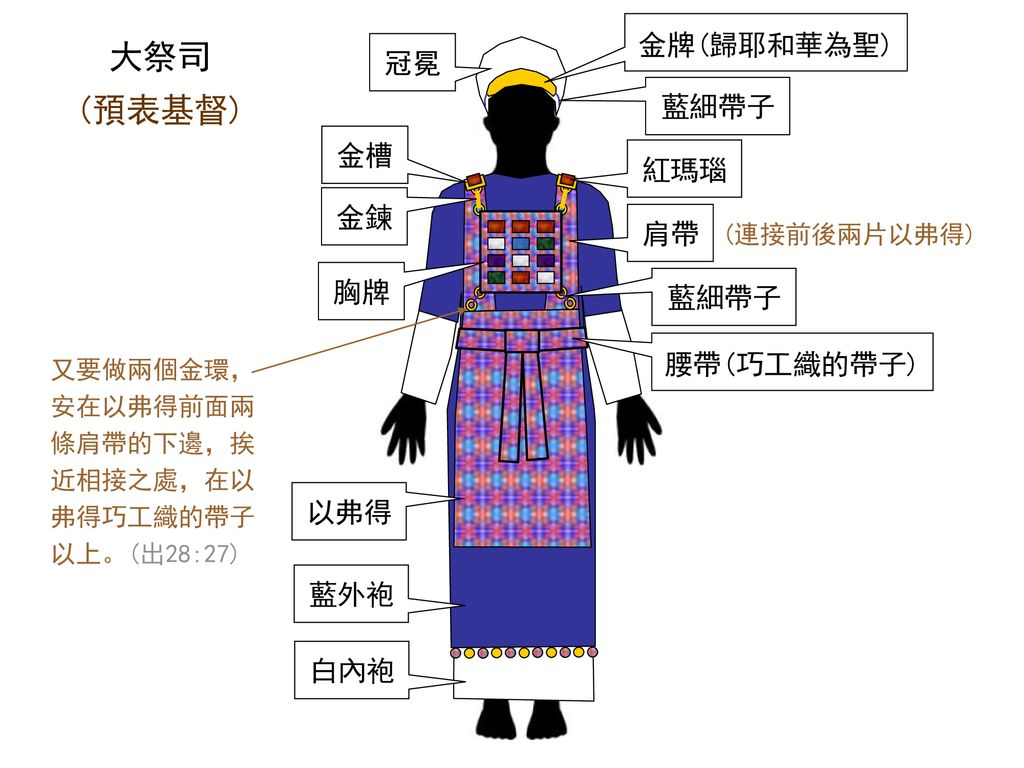
\includegraphics[height=2.5in]{AMoXiFigs/chuaiji/prest2}
       % \caption{}
    \end{subfigure}%
    ~ 
    \begin{subfigure}[b]{0.5\textwidth}
        \centering
        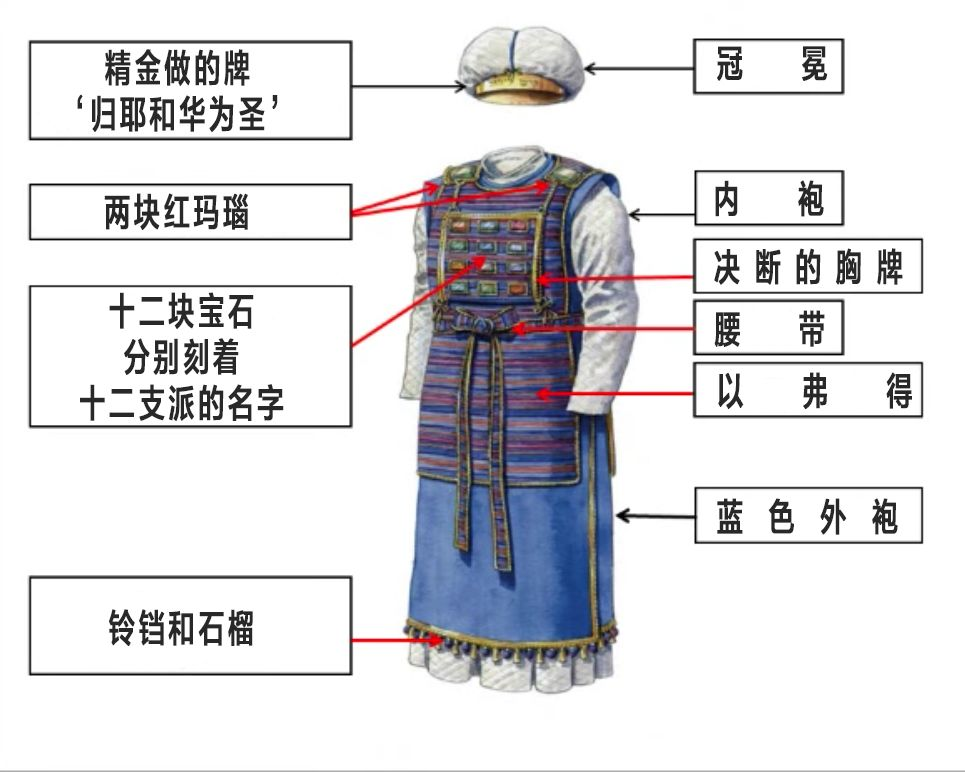
\includegraphics[height=2.5in]{AMoXiFigs/chuaiji/highprest}
      %  \caption{}
    \end{subfigure}
    \caption{祭司服饰图}
\end{figure*}

\subsubsubsection{命亞倫及其后裔為祭司并为其做聖衣 28:1-5}
\begin{itemize} 
\itemsep-.35em
\item 你要從以色列人中，使你的哥哥亞倫和他的兒子拿答、亞比戶、以利亞撒、以他瑪一同就近你，給我供祭司的職分。你要給你哥哥亞倫做聖衣為榮耀，為華美。 
\item 又要吩咐一切心中有智慧的，就是我用智慧的靈所充滿的，給亞倫做衣服，使他分別為聖，可以給我供祭司的職分。所要做的就是胸牌、以弗得、外袍、雜色的內袍、冠冕、腰帶，使你哥哥亞倫和他兒子穿這聖服，可以給我供祭司的職分。要用金線和藍色、紫色、朱紅色線並細麻去做
\end{itemize}
\begin{table}[H]
\centering
\begin{tabular}{|c|c|c| }
\hline
\hline
名稱 &材質　&　章節\\\hline
外袍 & 藍的& 28：31-35 \\\hline
胸牌&（1虎口 X 1虎口）胸牌貼在以弗得巧工織的帶子上&　28：15-30 \\\hline
以弗得&金線和藍色紫色朱紅色線、並撚的細麻&28：6-14　\\\hline
面牌&精金作、在上面刻著、歸耶和華為聖。這牌必在亞倫的額上&28：32-38　\\\hline
內袍&雜色細麻線織&　28：39\\\hline
冠冕&細麻布作&28：39　\\\hline
腰帶&繡花的手工作腰帶&28：39　\\\hline
褲子&細麻布。遮掩下體．褲子當從腰達到大腿&　28：42\\\hline
裹頭巾&亞倫的兒子用&　28：40\\\hline
\end{tabular}
\caption{祭司的服裝}
\end{table}

\subsubsubsection{做以弗得 28:6-14（39:2-7）}
\begin{wrapfigure}{r}{0.3\textwidth}
\vspace{-20pt}
\begin{center}
    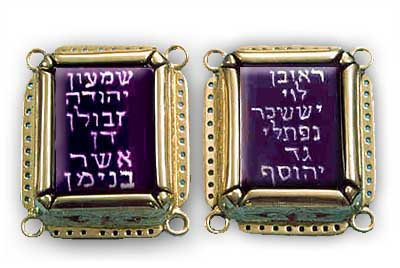
\includegraphics[width=0.3\textwidth]{AMoXiFigs/chuaiji/RedMaNao}
\end{center}
\vspace{-20pt}
  \caption{紅瑪瑙}
 \vspace{-10pt}
\end{wrapfigure}
他們要拿金線和藍色、紫色、朱紅色線並撚的細麻，用巧匠的手工做以弗得。以弗得當有兩條肩帶，接上兩頭，使它相連。其上巧工織的帶子，要和以弗得一樣的做法，用以束上，與以弗得接連一塊，要用金線和藍色、紫色、朱紅色線並撚的細麻做成。
要取兩塊紅瑪瑙，在上面刻以色列兒子的名字，六個名字在這塊寶石上，六個名字在那塊寶石上，都照他們生來的次序。要用刻寶石的手工，彷彿刻圖書，按著以色列兒子的名字刻這兩塊寶石，要鑲在金槽上。要將這兩塊寶石安在以弗得的兩條肩帶上，為以色列人做紀念石。亞倫要在兩肩上擔他們的名字，在耶和華面前作為紀念。
要用金子做二槽，又拿精金，用擰工彷彿擰繩子，做兩條鏈子，把這擰成的鏈子搭在二槽上。


\begin{table}[H]
\centering
\begin{tabular}{|c|c| }
\hline
\hline
材料 & 名稱  \\\hline
以弗得 & 細麻+線（金線，藍色，紫色，朱紅色）   \\\hline
兩條肩帶&細麻+線（金線，藍色，紫色，朱紅色）    \\\hline
兩塊紅瑪瑙&鑲金槽刻以色列兒子的名字 \\\hline
兩條鍊子&　精金、用擰工彷彿擰繩子　\\\hline
\end{tabular}
\caption{以弗得}
\end{table}



\subsubsubsection{做胸牌 28:15-30，39:8-21}
\iffalse
\begin{wraptable}{r}{7.5cm}
\begin{table}[H]
\centering
\begin{tabular}{|c|c|c|c| }
\hline
\hline
第一行 & 紅寶石&紅璧璽&紅玉  \\\hline
第二行&綠寶石&藍寶石&金鋼石  \\\hline
第三行&紫瑪瑙&白瑪瑙&紫晶。 \\\hline
第四行&　水蒼玉&紅瑪瑙&碧玉　\\\hline
\end{tabular}
\caption{胸牌}
\end{table}
\end{wrapfigure}
\fi
你要用巧匠的手工做一個決斷的胸牌。要和以弗得一樣的做法，用金線和藍色、紫色、朱紅色線並撚的細麻做成。這胸牌要四方的，疊為兩層，長一虎口，寬一虎口。要在上面鑲寶石四行：第一行是紅寶石、紅璧璽、紅玉，第二行是綠寶石、藍寶石、金鋼石，第三行是紫瑪瑙、白瑪瑙、紫晶，第四行是水蒼玉、紅瑪瑙、碧玉。這都要鑲在金槽中。
\begin{wrapfigure}{r}{0.3\textwidth}
\vspace{-20pt}
\begin{center}
    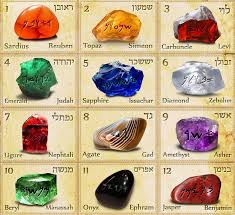
\includegraphics[width=0.3\textwidth]{AMoXiFigs/chuaiji/stones}
\end{center}
\vspace{-10pt}
  \caption{胸牌}
 \vspace{-10pt}
\end{wrapfigure}
這些寶石都要按著以色列十二個兒子的名字，彷彿刻圖書，刻十二個支派的名字。要在胸牌上用精金擰成如繩的鏈子。在胸牌上也要做兩個金環，安在胸牌的兩頭。要把那兩條擰成的金鏈子，穿過胸牌兩頭的環子。又要把鏈子的那兩頭接在兩槽上，安在以弗得前面肩帶上。要做兩個金環，安在胸牌的兩頭，在以弗得裡面的邊上。又要做兩個金環，安在以弗得前面兩條肩帶的下邊，挨近相接之處，在以弗得巧工織的帶子以上。要用藍細帶子把胸牌的環子與以弗得的環子繫住，使胸牌貼在以弗得巧工織的帶子上，不可與以弗得離縫。

亞倫進聖所的時候，要將決斷胸牌，就是刻著以色列兒子名字的，戴在胸前，在耶和華面前常做紀念。又要將烏陵和土明放在決斷的胸牌裡。亞倫進到耶和華面前的時候，要戴在胸前，在耶和華面前常將以色列人的決斷牌戴在胸前


\begin{table}[H]
    \begin{minipage}{.5\linewidth}
      \centering
       \begin{tabular}{|c|c|c|c| }
\hline
\hline
第一行 & 紅寶石&紅璧璽&紅玉  \\\hline
第二行&綠寶石&藍寶石&金鋼石  \\\hline
第三行&紫瑪瑙&白瑪瑙&紫晶。 \\\hline
第四行&　水蒼玉&紅瑪瑙&碧玉　\\\hline
\end{tabular}
   \caption{胸牌}
    \end{minipage}%
    \begin{minipage}{.5\linewidth}
      \centering    
     \begin{tabular}{|c|c| }
\hline
\hline
外袍 & 藍的  \\\hline
領口&口的周圍織出領邊  \\\hline
石榴&藍色+紫色+朱紅色線 \\\hline
金鈴鐺&金　\\\hline
\end{tabular}
%  \caption{以弗得外袍}
    \end{minipage} 
\end{table}


\subsubsubsection{製造以弗得外袍的規定 28:31-35（39:22-26）}
\begin{itemize} 
\itemsep-.35em
\item 你要做以弗得的外袍顏色全是藍的。袍上要為頭留一領口，口的周圍織出領邊來彷彿鎧甲的領口免得破裂
\item 袍子周圍底邊上要用藍色、紫色、朱紅色線做石榴，在袍子周圍的石榴中間要有金鈴鐺。一個金鈴鐺一個石榴，一個金鈴鐺一個石榴，在袍子周圍的底邊上。
\item 亞倫供職的時候要穿這袍子。他進聖所到耶和華面前以及出來的時候，袍上的響聲必被聽見使他不至死亡
\end{itemize}


\subsubsubsection{製造面牌的規定 28:36-38}
\begin{itemize} 
\itemsep-.35em
\item 你要用精金做一面牌，在上面按刻圖書之法刻著：歸耶和華為聖。要用一條藍細帶子將牌繫在冠冕的前面。
\item 這牌必在亞倫的額上，亞倫要擔當干犯聖物條例的罪孽，這聖物是以色列人在一切的聖禮物上所分別為聖的。這牌要常在他的額上，使他們可以在耶和華面前蒙悅納。
\end{itemize}

\subsubsubsection{製造內袍冠冕腰帶裹頭巾褲子 28:39-43（39:27-29）}
\begin{itemize} 
\itemsep-.35em
\item 要用雜色細麻線織內袍，用細麻布做冠冕，又用繡花的手工做腰帶。你要為亞倫的兒子做內袍、腰帶、裹頭巾，為榮耀，為華美。要把這些給你的哥哥亞倫和他的兒子穿戴，又要膏他們，將他們分別為聖，好給我供祭司的職分。 
\item 要給他們做細麻布褲子，遮掩下體，褲子當從腰達到大腿。亞倫和他兒子進入會幕，或就近壇，在聖所供職的時候必穿上，免得擔罪而死。這要為亞倫和他的後裔做永遠的定例
\end{itemize}

\subsubsection{祭司分别为圣的禮仪 29}
\subsubsubsection{祭司承接聖職的穿戴 29:1-9 }
\begin{itemize} 
\itemsep-.35em
\item 你使亞倫和他兒子成聖，給我供祭司的職分，要如此行。
\begin{itemize} 
\itemsep-.35em
\item 献祭：取一隻\underline{公牛犢}，兩隻無殘疾的\underline{公綿羊}，\underline{無酵餅}和\underline{調油的無酵餅}，與\underline{抹油的無酵薄餅}，這都要用細麥麵做成。這餅要裝在一個筐子裡，連筐子帶來，又把公牛和兩隻公綿羊牽來。
\item 要使亞倫和他兒子到會幕門口來用水洗身。 
\begin{itemize} 
\itemsep-.35em
\item 要給亞倫穿上內袍和以弗得的外袍並以弗得，又戴上胸牌，束上以弗得巧工織的帶子。 6 把冠冕戴在他頭上，將聖冠加在冠冕上，就把膏油倒在他頭上膏他。 
\item 要叫他的兒子來，給他們穿上內袍。 
\item 給亞倫和他兒子束上腰帶，包上裹頭巾，
\end{itemize} 
\end{itemize}
\item 他們就憑永遠的定例得了祭司的職任。又要將亞倫和他兒子分別為聖
\end{itemize}


\subsubsubsection{承接聖職的贖罪祭-公牛 29:10-14 （利8:14-17）}
\begin{itemize} 
\itemsep-.35em
\item 你要把公牛牽到會幕前，亞倫和他兒子要按手在公牛的頭上。 
\item 你要在耶和華面前，在會幕門口，宰這公牛。要取些公牛的血，用指頭抹在壇的四角上，把血都倒在壇腳那裡。要把一切蓋臟的脂油與肝上的網子，並兩個腰子和腰子上的脂油，都燒在壇上。只是公牛的皮、肉、糞都要用火燒在營外。這牛是\underline{贖罪祭}
\end{itemize}

\subsubsubsection{承接聖職的燔祭-一隻公綿羊 29:15-18 （利8:18-21）}
\begin{itemize} 
\itemsep-.35em
\item 你要牽一隻公綿羊來，亞倫和他兒子要按手在這羊的頭上。 
\item 要宰這羊，把血灑在壇的周圍。要把羊切成塊子，洗淨五臟和腿，連塊子帶頭，都放在一處。要把全羊燒在壇上，是給耶和華獻的\underline{燔祭}，是獻給耶和華為馨香的\underline{火祭}
\end{itemize}

\subsubsubsection{承接聖職的公綿羊-搖祭及舉祭 29:19-25 （利8:22-29）}
\begin{itemize} 
\itemsep-.35em
\item 你要將那一隻公綿羊牽來，亞倫和他兒子要按手在羊的頭上。你要宰這羊，取點血抹在亞倫的右耳垂上和他兒子的右耳垂上，又抹在他們右手的大拇指上和右腳的大拇指上，並要把血灑在壇的四圍。你要取點膏油和壇上的血，彈在亞倫和他的衣服上，並他兒子和他兒子的衣服上，\underline{他們和他們的衣服就一同成聖} 。 
\item 搖祭放在燔祭上燒=馨香的火祭
\begin{itemize} 
\itemsep-.35em
\item 你要取這羊的脂油和肥尾巴，並蓋臟的脂油與肝上的網子，兩個腰子和腰子上的脂油並右腿，這是承接聖職所獻的羊。再從耶和華面前裝無酵餅的筐子中取一個餅，一個調油的餅和一個薄餅，都放在亞倫的手上和他兒子的手上，作為\underline{搖祭}，在耶和華面前搖一搖。
\item 要從他們手中接過來，\underline{燒在}耶和華面前壇上的\underline{燔祭}上，是獻給耶和華為馨香的\underline{火祭}。
\end{itemize}
\end{itemize}

\subsubsubsection{承接聖職的其他禮儀 29:29-37 （利8:30-35）}
\begin{itemize} 
\itemsep-.35em
\item 亞倫的聖衣要留給他的子孫，可以穿著受膏，又穿著承接聖職。他的子孫接續他當祭司的，每逢進會幕在聖所供職的時候，要穿七天。
\item 你要將承接聖職所獻公羊的肉煮在聖處。亞倫和他兒子要在會幕門口吃這羊的肉和筐內的餅。他們吃那些贖罪之物，好承接聖職，使他們成聖；只是外人不可吃，因為這是聖物。那承接聖職所獻的肉或餅，若有一點留到早晨，就要用火燒了，不可吃這物，因為是聖物。
\item 你要這樣照我一切所吩咐的，向亞倫和他兒子行承接聖職的禮七天。每天要獻公牛一隻為贖罪祭。你潔淨壇的時候，壇就潔淨了，且要用膏抹壇，使壇成聖。要潔淨壇七天，使壇成聖，壇就成為至聖。凡挨著壇的都成為聖
\end{itemize}


\subsubsubsection{祭司每天當獻的祭物 29:38-46 }
\begin{itemize} 
\itemsep-.35em
\item 你每天所要獻在壇上的就是兩隻一歲的羊羔，早晨要獻這一隻，黃昏的時候要獻那一隻。和這一隻羊羔同獻的，要用細麵伊法十分之一與搗成的油一欣四分之一調和，又用酒一欣四分之一作為奠祭。那一隻羊羔要在黃昏的時候獻上，照著早晨的素祭和奠祭的禮辦理，作為獻給耶和華馨香的火祭。
\item 這要在耶和華面前，會幕門口，做你們世世代代常獻的燔祭。我要在那裡與你們相會，和你們說話。我要在那裡與以色列人相會，會幕就要因我的榮耀成為聖。我要使會幕和壇成聖，也要使亞倫和他的兒子成聖，給我供祭司的職分。
\item 我要住在以色列人中間，做他們的神。他們必知道我是耶和華他們的神，是將他們從埃及地領出來的，為要住在他們中間。我是耶和華他們的神
\end{itemize}
\begin{table}[H]
\centering
\begin{tabular}{|c|c|c|c|c|c|c| }
\hline
\hline
天&贖罪祭 & 燔祭&承接聖職獻的祭 &素祭 &搖祭 & 舉祭\\\hline
1&公牛& 公綿羊（1) &公綿羊（1) & 無酵餅 &無酵餅（1) & 承接聖職公綿羊的腿\\\hline
 &&   & & 調油的無酵餅  & 調油的餅 （1) & \\\hline
 & &   & & 抹油的無酵薄餅 & 薄餅（1) &\\\hline
& &   & &   & 承接聖職公綿羊的胸 & \\\hline
2& 公牛&   & &   &   & \\\hline
3&公牛 &   & &   &   & \\\hline
4&公牛 &   & &   &   & \\\hline
5&公牛 &   & &   &   & \\\hline
6&公牛 &   & &   &   & \\\hline
7&公牛 &   & &   &  & \\\hline
\end{tabular}
\caption{承接聖職獻的7天祭}
\end{table}


\subsubsection{其它会幕物品制作服事條例 30-31}
\subsubsubsection{造香壇的條例 30:1-6，37:25-28}
\begin{itemize} 
\itemsep-.35em
\item 你要用皂莢木做一座燒香的壇。這壇要四方的，長一肘，寬一肘，高二肘。壇的四角要與壇接連一塊。要用精金把壇的上面與壇的四圍並壇的四角包裹
\item 又要在壇的四圍鑲上金牙邊。要做兩個金環安在牙子邊以下，在壇的兩旁兩根橫撐上，作為穿槓的用處，以便抬壇。要用皂莢木做槓，用金包裹。
\item 要把壇放在法櫃前的幔子外，對著法櫃上的施恩座，就是我要與你相會的地方。 
\end{itemize}

\subsubsubsection{亞倫在壇上的服事條例 30:7-10}
\vspace*{-5mm}
 \begin{itemize} 
\itemsep-.35em
\item 亞倫在壇上要燒馨香料做的香，每早晨他收拾燈的時候，要燒這香。黃昏點燈的時候，他要在耶和華面前燒這香，作為世世代代常燒的香。在這壇上不可奉上異樣的香，不可獻燔祭、素祭，也不可澆上奠祭。
\item 亞倫一年一次要在壇的角上行贖罪之禮。他一年一次要用贖罪祭牲的血在壇上行贖罪之禮，作為世世代代的定例。這壇在耶和華面前為至聖。
\end{itemize}

\subsubsubsection{每人當獻贖命之價 30:11-16 （37:25-28）}
\begin{itemize} 
\itemsep-.35em
\item 耶和華曉諭摩西說：「你要按以色列人被數的計算總數，你數的時候，他們各人要為自己的生命把贖價奉給耶和華，免得數的時候在他們中間有災殃。凡過去歸那些被數之人的，每人要按聖所的平，拿銀子半舍客勒，這半舍客勒是奉給耶和華的禮物，一舍客勒是二十季拉。凡過去歸那些被數的人，從二十歲以外的，要將這禮物奉給耶和華。
\item 他們為贖生命將禮物奉給耶和華，富足的不可多出，貧窮的也不可少出，各人要出半舍客勒。你要從以色列人收這贖罪銀，作為會幕的使用，可以在耶和華面前為以色列人做紀念，贖生命。
\end{itemize}

\subsubsubsection{造銅盆的規定 30:17-21 （38:8）}
\begin{itemize} 
\itemsep-.35em
\item 耶和華曉諭摩西說：你要用銅做洗濯盆和盆座，以便洗濯。要將盆放在會幕和壇的中間，在盆裡盛水。
\item 亞倫和他的兒子要在這盆裡洗手洗腳。他們進會幕，或是就近壇前供職給耶和華\underline{獻火祭}的時候，\underline{必用水洗濯}，免得死亡。他們洗手洗腳，就免得死亡。這要做亞倫和他後裔世世代代永遠的定例。
\end{itemize}


\subsubsubsection{製作聖膏油的規定 30:22-33}
\begin{wraptable}{r}{4.2cm}
\vspace*{-\baselineskip}
\begin{tabular}{ll }
\hline
\hline
聖膏油製作& 份量 \\\hline
沒藥 & 500舍客勒 \\\hline
香肉桂&250舍客勒  \\\hline
菖蒲&250舍客勒   \\\hline
桂皮&500舍客勒   \\\hline
橄欖油&1欣 \\\hline
\end{tabular}
\caption{聖膏油的規定}
\end{wraptable}
耶和華曉諭摩西說： 「你要取上品的香料，就是流質的沒藥五百舍客勒，香肉桂一半，就是二百五十舍客勒，菖蒲二百五十舍客勒，桂皮五百舍客勒，都按著聖所的平，又取橄欖油一欣，按做香之法調和做成聖膏油。\\
要用這膏油抹會幕和法櫃，桌子與桌子的一切器具，燈臺和燈臺的器具並香壇，燔祭壇和壇的一切器具，洗濯盆和盆座。要使這些物成為聖，好成為至聖，凡挨著的都成為聖。要膏亞倫和他的兒子，使他們成為聖，可以給我供祭司的職分。\\
你要對以色列人說：『這油，我要世世代代以為聖膏油。不可倒在別人的身上，也不可按這調和之法做與此相似的。這膏油是聖的，你們也要以為聖。凡調和與此相似的，或將這膏膏在別人身上的，這人要從民中剪除。』



\iffalse
\begin{table}[H]
    \begin{subtable}{.5\linewidth}
 \centering  
\begin{tabular}{ll }
\hline
\hline
聖膏油製作& 份量 \\\hline
沒藥 & 500舍客勒 \\\hline
香肉桂&250舍客勒  \\\hline
菖蒲&250舍客勒   \\\hline
桂皮&500舍客勒   \\\hline
橄欖油&1欣 \\\hline
\end{tabular}
\caption{聖膏油和聖香的規定}
    \end{subtable}%
    \begin{subtable}{.5\linewidth}
      \centering    
    \begin{tabular}{ll}
\hline
\hline
聖香製作 &份量\\\hline
 拿他弗 & 1份  \\\hline
  施喜列 &1份 \\\hline
 喜利比拿 &1份  \\\hline
 淨乳香 &1份 \\\hline
 鹽 &\\\hline
\end{tabular}
   \caption{聖香製作}
    \end{subtable} 
\end{table}
\fi

\subsubsubsection{製作聖香的規定 30:34-38}
\begin{wraptable}{r}{5cm}
%\vspace*{-\baselineskip}
\vspace*{-10mm}
   \begin{tabular}{ll}
\hline
\hline
聖香製作 &份量\\\hline
 拿他弗 & 1份  \\\hline
  施喜列 &1份 \\\hline
 喜利比拿 &1份  \\\hline
 淨乳香 &1份 \\\hline
 鹽 &\\\hline
\end{tabular}
\caption{聖香製作}
\end{wraptable}
耶和華吩咐摩西說：「你要取馨香的香料，就是拿他弗、施喜列、喜利比拿，這馨香的香料和淨乳香各樣要一般大的分量。你要用這些加上鹽，按做香之法做成清淨聖潔的香。這香要取點搗得極細，放在會幕內法櫃前，我要在那裡與你相會。\\
你們要以這香為至聖。你們不可按這調和之法為自己做香，要以這香為聖，歸耶和華。凡做香和這香一樣，為要聞香味的，這人要從民中剪除。


\subsubsubsection{神提名比撒列,亞何利亞伯造會幕 31:1-11 （35:30-35）}
%\begin{wraptable}{r}{7.5cm}
\begin{table}[H]
\vspace*{-\baselineskip}
%\vspace*{1.0cm}
\center
\begin{tabular}{ c c c c }
\toprule
支派 & 爺爺名字 & 父親名字& 技工 \\\hline
猶大&戶珥  &  烏利 & 比撒列\\\hline
但&  & 亞希撒抹& 亞何利亞伯 \\\hline
\end{tabular}
\caption{技工比撒列,亞何利亞伯}
\end{table} 
%\end{wraptable}
%\vspace*{-\baselineskip}
耶和華曉諭摩西說：「看哪，猶大支派中，戶珥的孫子、烏利的兒子比撒列，我已經提他的名召他。我也以我的靈充滿了他，使他有智慧，有聰明，有知識，能做各樣的工， 能想出巧工，用金、銀、銅製造各物，又能刻寶石，可以鑲嵌，能雕刻木頭，能做各樣的工。\\
我分派但支派中亞希撒抹的兒子亞何利亞伯與他同工。\underline{\textcolor{blue}{凡}心裡有智慧的，我\textcolor{blue}{更}使他們有智慧，\textcolor{blue}{能}做我一切所吩咐的}，就是會幕和法櫃，並其上的施恩座，與會幕中一切的器具，桌子和桌子的器具，精金的燈臺和燈臺的一切器具並香壇， 燔祭壇和壇的一切器具，並洗濯盆與盆座，精工做的禮服，和祭司亞倫並他兒子用以供祭司職分的聖衣，膏油和為聖所用馨香的香料。他們都要照我一切所吩咐的去做。」
%\end{itemize}


\subsubsubsection{當守安息日為證 31:12-18}
\begin{itemize}
\itemsep-.35em
\item 耶和華曉諭摩西說：「你要吩咐以色列人說：『你們務要守我的安息日，因為這是你我之間世世代代的證據，使你們知道我\underline{耶和華是叫你們成為聖的。所以你們要守安息日，以為聖日}。凡干犯這日的，必要把他治死；凡在這日做工的，必從民中剪除。六日要做工，但第七日是安息聖日，是向耶和華守為聖的。凡在安息日做工的，必要把他治死。故此，以色列人要世世代代守安息日為永遠的約。這是我和以色列人永遠的證據，因為六日之內\underline{耶和華造天地，第七日便安息舒暢}。』」
\item 耶和華在西奈山和摩西說完了話，就把兩塊法版交給他，是神用指頭寫的石版。
\end{itemize}

\subsection{摩西四次上山為百姓拜金牛犢代求 32-34}
\subsubsection{亞倫造犢 32:1-6}
\begin{itemize}
\itemsep-.35em
\item 百姓見摩西遲延不下山，就大家聚集到亞倫那裡，對他說：「起來，為我們做神像，可以在我們前面引路，因為領我們出埃及地的那個摩西，我們不知道他遭了什麼事。」 
\item 亞倫對他們說：「你們去摘下你們妻子、兒女耳上的金環，拿來給我。」
\begin{itemize}
\itemsep-.35em
\item 百姓就都摘下他們耳上的金環，拿來給亞倫。 
 \item 亞倫從他們手裡接過來，鑄了一隻牛犢，用雕刻的器具做成。他們就說：「以色列啊，這是領你出埃及地的神！」亞倫看見，就在牛犢面前築壇，且宣告說：「明日要向耶和華守節。」 
\item 次日清早，百姓起來獻燔祭和平安祭，就坐下吃喝，起來玩耍。
\end{itemize}
\end{itemize}

\subsubsection{摩西第一次為百姓代求 32:7-14}
\begin{table}[H]
\begin{threeparttable}
\begin{tabular}{@{}p{0.4\textwidth}*{4}{L{\dimexpr0.7\linewidth-10\tabcolsep\relax}}@{}}
\toprule
神 &  摩西 \\\hline
耶和華吩咐摩西說：「下去吧，因為你的百姓，就是你從埃及地領出來的，已經敗壞了。他們快快偏離了我所吩咐的道，為自己鑄了一隻牛犢，向它下拜獻祭，說：『以色列啊，這就是領你出埃及地的神！』」&\tabularnewline\hline
耶和華對摩西說：「我看這百姓真是硬著頸項的百姓。你且由著我，我要向他們發烈怒，將他們滅絕，使你的後裔成為大國。」&摩西便懇求耶和華他的神說：「耶和華啊，你為什麼向你的百姓發烈怒呢？這百姓是你用大力和大能的手從埃及地領出來的。為什麼使埃及人議論說『他領他們出去，是要降禍於他們，把他們殺在山中，將他們從地上除滅』？求你轉意，不發你的烈怒；後悔，不降禍與你的百姓。求你記念你的僕人亞伯拉罕、以撒、以色列，你曾指著自己起誓說：『我必使你們的後裔像天上的星那樣多，並且我所應許的這全地，必給你們的後裔，他們要永遠承受為業。』」\tabularnewline\hline
於是耶和華後悔，不把所說的禍降於他的百姓&\tabularnewline
\bottomrule
\end{tabular}
%\caption{摩西第一次為百姓代求}
\end{threeparttable}
\end{table} 


\subsubsection{摩西怒摔法版 32:15-29}
\begin{itemize}
\itemsep-.35em
\item 摩西轉身下山手裡拿著兩塊法版。這版是兩面寫的這面那面都有字，是神的工作，字是神寫的刻在版上。約書亞一聽見百姓呼喊的聲音，就對摩西說：「在營裡有爭戰的聲音。」摩西說：「這不是人打勝仗的聲音，也不是人打敗仗的聲音，我所聽見的乃是人歌唱的聲音。」
\item 摩西挨近營前，就看見牛犢，又看見人跳舞，便發烈怒，把兩塊版扔在山下摔碎了，又將他們所鑄的牛犢用火焚燒，磨得粉碎，撒在水面上，叫以色列人喝。摩西對亞倫說：「這百姓向你做了什麼？你竟使他們陷在大罪裡！」亞倫說：「求我主不要發烈怒。這百姓專於作惡，是你知道的。他們對我說：『你為我們做神像，可以在我們前面引路，因為領我們出埃及地的那個摩西，我們不知道他遭了什麼事。』我對他們說：『凡有金環的，可以摘下來。』他們就給了我，我把金環扔在火中，這牛犢便出來了。」
\item 三千百姓被利未的子孫殺死
\begin{table}[H]
\begin{threeparttable}
\begin{tabular}{@{}p{0.6\textwidth}*{4}{L{\dimexpr0.5\linewidth-10\tabcolsep\relax}}@{}}
\toprule
摩西 & 利未的子孫 \\\hline
摩西見百姓放肆（亞倫縱容他們，使他們在仇敵中間被譏刺），就站在營門中，說：「凡屬耶和華的，都要到我這裡來！」&於是利未的子孫都到他那裡聚集。\tabularnewline\hline
他對他們說：「耶和華以色列的神這樣說：『你們各人把刀跨在腰間，在營中往來，從這門到那門，各人殺他的弟兄與同伴並鄰舍。』」 &利未的子孫照摩西的話行了。那一天百姓中被殺的約有三千\tabularnewline\hline
摩西說：「今天你們要自潔，歸耶和華為聖，各人攻擊他的兒子和弟兄，使耶和華賜福於你們。」 &\tabularnewline
\bottomrule
\end{tabular}
\caption{三千百姓被利未的子孫殺死}
\end{threeparttable}
\end{table} 
\end{itemize}

\subsubsection{摩西第二次為百姓代求 32:30-33:3}
\begin{table}[H]
\begin{threeparttable}
\begin{tabular}{@{}p{0.4\textwidth}*{4}{L{\dimexpr0.6\linewidth-10\tabcolsep\relax}}@{}}
\toprule
摩西 &  神 \\\hline
到了第二天，摩西對百姓說:你們犯了大罪，我如今要上耶和華那裡去，或者可以為你們贖罪&\tabularnewline\hline
摩西回到耶和華那裡，說：「唉！這百姓犯了大罪，為自己做了金像。倘或你肯赦免他們的罪——不然，求你從你所寫的冊上塗抹我的名。」&耶和華對摩西說：「誰得罪我，我就從我的冊上塗抹誰的名。現在你去領這百姓，往我所告訴你的地方去，我的使者必在你前面引路，只是到我追討的日子，我必追討他們的罪。」\tabularnewline\hline
&耶和華殺百姓的緣故是因他們同亞倫做了牛犢。\tabularnewline\hline
&耶和華吩咐摩西說：「我曾起誓應許亞伯拉罕、以撒、雅各說：『要將迦南地賜給你的後裔。』現在你和你從埃及地所領出來的百姓，要從這裡往那地去。我要差遣使者在你前面，攆出迦南人、亞摩利人、赫人、比利洗人、希未人、耶布斯人領你到那流奶與蜜之地。我自己不同你們上去，因為你們是硬著頸項的百姓，恐怕我在路上把你們滅絕。」\tabularnewline
\bottomrule
\end{tabular}
%\caption{摩西第二次為百姓代求}
\end{threeparttable}
\end{table} 

\subsubsection{百姓除淨身上佩戴裝飾 33:4-6}
\begin{itemize}
\itemsep-.35em
\item 百姓聽見這凶信就悲哀，也沒有人佩戴裝飾。 
\item 耶和華對摩西說：「你告訴以色列人說：『耶和華說：你們是硬著頸項的百姓，我若一霎時臨到你們中間，必滅絕你們。現在你們要把身上的裝飾摘下來，使我可以知道怎樣待你們。』」 
\item 以色列人從住何烈山以後，就把身上的裝飾摘得乾淨
\end{itemize}

\subsubsection{摩西與神會面的會幕——支搭在的營外帳篷 33:7-11}
\begin{itemize}
\itemsep-.35em
\item 摩西素常將帳篷支搭在營外，離營卻遠，他稱這帳篷為會幕。凡求問耶和華的，就到營外的會幕那裡去。 
\begin{itemize}
\itemsep-.35em
\item 當摩西出營到會幕去的時候，百姓就都起來，各人站在自己帳篷的門口，望著摩西，直等到他進了會幕。
 \item 摩西進會幕的時候，雲柱降下來，立在會幕的門前，耶和華便與摩西說話。
\item 眾百姓看見雲柱立在會幕門前，就都起來，各人在自己帳篷的門口下拜。
\item 耶和華與摩西面對面說話，好像人與朋友說話一般。
\end{itemize}
\item 摩西轉到營裡去，唯有他的幫手，一個少年人嫩的兒子約書亞，不離開會幕。
\end{itemize}


\subsubsection{摩西求耶和華同往,并蒙恩见神的荣耀 33:12-23}
\begin{table}[H]
\begin{threeparttable}
\begin{tabular}{@{}p{0.4\textwidth}*{4}{L{\dimexpr0.7\linewidth-10\tabcolsep\relax}}@{}}
\toprule
摩西的祈祷 &  神的应许 \\\hline
摩西對耶和華說：「你吩咐我說：『將這百姓領上去』，卻沒有叫我知道你要打發誰與我同去，只說：『我按你的名認識你，你在我眼前也蒙了恩。』 我如今若在你眼前蒙恩，求你將你的道指示我，使我可以認識你，好在你眼前蒙恩。求你想到這民是你的民。」&耶和華說：「我必親自和你同去，使你得安息。」\tabularnewline\hline
摩西說：「你若不親自和我同去，就不要把我們從這裡領上去。人在何事上得以知道我和你的百姓在你眼前蒙恩呢？豈不是因你與我們同去，使我和你的百姓與地上的萬民有分別嗎？」&耶和華對摩西說：「你這所求的我也要行，因為你在我眼前蒙了恩，並且我按你的名認識你。」 \tabularnewline\hline
摩西說：「求你顯出你的榮耀給我看。」&耶和華說：「我要顯我一切的恩慈，在你面前經過，宣告我的名。我要恩待誰就恩待誰，要憐憫誰就憐憫誰。」 \tabularnewline\hline
&又說：「你不能看見我的面，因為人見我的面不能存活。」 \tabularnewline\hline
&耶和華說：「看哪，在我這裡有地方，你要站在磐石上。我的榮耀經過的時候，我必將你放在磐石穴中，用我的手遮掩你，等我過去。然後我要將我的手收回，你就得見我的背，卻不得見我的面。」 \tabularnewline
\bottomrule
\end{tabular}
\caption{摩西求耶和華同往,并蒙恩见神的荣耀}
\end{threeparttable}
\end{table} 

\subsubsection{摩西復上西奈山，新鑿兩塊石版 34:1-4 （申10:1-5）}
耶和華吩咐摩西說：「你要鑿出兩塊石版，和先前你摔碎的那版一樣，其上的字我要寫在這版上。明日早晨，你要預備好了，上西奈山，在山頂上站在我面前。誰也不可和你一同上去，遍山都不可有人，在山根也不可叫羊群牛群吃草。」 \\
摩西就鑿出兩塊石版，和先前的一樣。清晨起來，照耶和華所吩咐的上西奈山去，手裡拿著兩塊石版。

\subsubsection{耶和華宣告自己的名 34:5-9}
耶和華在雲中降臨，和摩西一同站在那裡，宣告耶和華的名。耶和華在他面前宣告說：「耶和華，耶和華，是有憐憫有恩典的神，不輕易發怒，並有豐盛的慈愛和誠實。為千萬人存留慈愛，赦免罪孽、過犯和罪惡；萬不以有罪的為無罪，必追討他的罪，自父及子，直到三四代。」 \\
摩西急忙伏地下拜，說：「主啊，我若在你眼前蒙恩，求你在我們中間同行，因為這是硬著頸項的百姓。又求你赦免我們的罪孽和罪惡，以我們為你的產業。」

\subsubsection{耶和華和立約，并禁止百姓拜別神 34:10-17}
耶和華說：「我要立約，要在百姓面前行奇妙的事，是在遍地萬國中所未曾行的。在你四圍的外邦人就要看見耶和華的作為，因我向你所行的是可畏懼的事。我今天所吩咐你的，你要謹守。我要從你面前攆出亞摩利人、迦南人、赫人、比利洗人、希未人、耶布斯人。\\
你要謹慎，\underline{不可}與你所去那地的居民立約，恐怕成為你們中間的網羅；卻要拆毀他們的祭壇，打碎他們的柱像，砍下他們的木偶。\underline{不可}敬拜別神，因為耶和華是忌邪的神，名為忌邪者。只怕你與那地的居民立約，百姓隨從他們的神，就行邪淫，祭祀他們的神，有人叫你，你便吃他的祭物；又為你的兒子娶他們的女兒為妻，他們的女兒隨從她們的神，就行邪淫，使你的兒子也隨從她們的神行邪淫。\underline{不可}為自己鑄造神像。

\subsubsection{守除酵節,安息日,七七節,收藏節 34:16-26}
你要守\underline{除酵節}，照我所吩咐你的，在亞筆月內所定的日期吃無酵餅七天，因為你是這亞筆月內出了埃及。凡\underline{頭生}的都是我的，一切牲畜頭生的，無論是牛是羊，公的都是我的。頭生的驢要用羊羔代贖，若不代贖就要打折牠的頸項。凡頭生的兒子都要贖出來。誰也不可空手朝見我。\\
你六日要做工，第七日要安息；雖在耕種收割的時候，也要安息。在收割初熟麥子的時候要守\underline{七七節}，又在年底要守\underline{收藏節}。你們一切男丁要一年三次朝見主耶和華以色列的神。我要從你面前趕出外邦人，擴張你的境界。你一年三次上去朝見耶和華你神的時候，必沒有人貪慕你的地土。\\
你不可將我祭物的血和有酵的餅一同獻上，逾越節的祭物也不可留到早晨。地裡首先初熟之物要送到耶和華你神的殿。不可用山羊羔母的奶煮山羊羔。\\

\subsubsection{摩西四十晝夜不吃飯不喝水 34:27-28}
耶和華吩咐摩西說：「你要將這些話寫上，因為我是按這話與你和以色列人立約。」摩西在耶和華那裡四十晝夜，也不吃飯，也不喝水。耶和華將這約的話，就是十條誡，寫在兩塊版上。

\subsubsection{摩西面容發光 34:16-26}
摩西手裡拿著兩塊法版下西奈山的時候，不知道自己的面皮因耶和華和他說話就發了光。亞倫和以色列眾人看見摩西的面皮發光，就怕挨近他。摩西叫他們來，於是亞倫和會眾的官長都到他那裡去，摩西就與他們說話。隨後以色列眾人都近前來，他就把耶和華在西奈山與他所說的一切話都吩咐他們。摩西與他們說完了話，就用帕子蒙上臉。但摩西進到耶和華面前與他說話就揭去帕子，及至出來的時候，便將耶和華所吩咐的告訴以色列人。以色列人看見摩西的面皮發光。摩西又用帕子蒙上臉，等到他進去與耶和華說話，就揭去帕子

\subsection{摩西传神的話，造會幕和祭司服 35-40}
\subsubsection{守安息日之例 35:1-2}
摩西招聚以色列全會眾，對他們說：「這是耶和華所吩咐的話，叫你們照著行。六日要做工，第七日乃為聖日，\underline{當向耶和華守為安息聖日}。凡這日之內做工的，必把他治死。當安息日，不可在你們一切的住處生火。」

\subsubsection{呼召會眾獻禮物 35:4-9 （25:1-7）}
\begin{wraptable}{r}{10.5cm}
%\begin{table}[!hbp]
%\centering
%\vspace*{-\baselineskip}
\vspace*{-1cm}
\begin{tabular}{|c|c| }
\hline
\hline
材料 & 名稱  \\\hline
金屬 & 金、銀、銅    \\\hline
線類&藍色、紫色、朱紅色線、細麻、山羊毛  \\\hline
皮類&染紅的公羊皮、海狗皮 \\\hline
木類&　皂莢木 　\\\hline
油、香料&點燈的油並做膏油和香的香料　\\\hline
寶石&紅瑪瑙與別樣的寶石，可以鑲嵌在以弗得和胸牌上 \\\hline
\end{tabular}
\caption{呼召會眾奉獻的物}
%\end{table}
\end{wraptable} 
摩西對以色列全會眾說：「耶和華所吩咐的是這樣：你們中間要拿禮物獻給耶和華，凡樂意獻的，可以拿耶和華的禮物來，就是金，銀，銅，藍色、紫色、朱紅色線，細麻，山羊毛，染紅的公羊皮，海狗皮，皂莢木，點燈的油，並做膏油和香的香料，紅瑪瑙與別樣的寶石，可以鑲嵌在以弗得和胸牌上。

\subsubsection{呼召有智慧的来做神的工及工作内容 35:10-19 (39:32-41)}
你們中間凡心裡有智慧的，都要來做耶和華一切所吩咐的，就是帳幕和帳幕的罩篷，並帳幕的蓋、鉤子、板、閂、柱子、帶卯的座，櫃和櫃的槓，施恩座和遮掩櫃的幔子，桌子和桌子的槓與桌子的一切器具，並陳設餅，燈臺和燈臺的器具，燈盞並點燈的油，香壇和壇的槓，膏油和馨香的香料，並帳幕門口的簾子，燔祭壇和壇的銅網，壇的槓並壇的一切器具，洗濯盆和盆座，院子的帷子和帷子的柱子，帶卯的座和院子的門簾，帳幕的橛子並院子的橛子和這兩處的繩子，精工做的禮服和祭司亞倫並他兒子在聖所用以供祭司職分的聖衣。

\subsubsection{會眾回应獻禮物的呼召 35:20-29}
以色列全會眾從摩西面前退去。凡心裡受感和甘心樂意的，都拿耶和華的禮物來，用以做會幕和其中一切的使用，又用以做聖衣。凡心裡樂意獻禮物的，連男帶女，各將金器，就是胸前針、耳環 (鼻環)、打印的戒指和手釧，帶來獻給耶和華。凡有藍色、紫色、朱紅色線，細麻，山羊毛，染紅的公羊皮，海狗皮的，都拿了來。凡獻銀子和銅給耶和華為禮物的，都拿了來。凡有皂莢木可做什麼使用的，也拿了來。凡心中有智慧的婦女，親手紡線，把所紡的藍色、紫色、朱紅色線和細麻都拿了來。凡有智慧心裡受感的婦女，就紡山羊毛。眾官長把紅瑪瑙和別樣的寶石，可以鑲嵌在以弗得與胸牌上的，都拿了來，又拿香料做香，拿油點燈，做膏油。以色列人，無論男女，凡甘心樂意獻禮物給耶和華的，都將禮物拿來，做耶和華藉摩西所吩咐的一切工。

\subsubsection{呼召做会幕的技工 35:30-36:2 (31:2-6)}
\begin{wraptable}{r}{12.5cm}
%\begin{table}[H]
\vspace*{-\baselineskip}
%\vspace*{3.0cm}
\center
\begin{tabular}{ c c c c l }
\toprule
支派 &爺爺 &父親名字&技工 &擅长\\\hline
猶大&戶珥  &烏利 &比撒列  &能做金銀銅器，刻嵌寶石，雕刻木頭\\\hline
但&  &亞希撒抹&亞何利亞伯 &藍紫朱紅線和細麻繡花、機匠的工\\\hline
\end{tabular}
\caption{技工比撒列,亞何利亞伯}
%\end{table} 
\end{wraptable}
摩西對以色列人說：「\textcolor{blue}{猶大}支派中，戶珥的孫子、烏利的兒子\textcolor{blue}{比撒列}，耶和華已經提他的名召他，又以神的靈充滿了他，使他有智慧、聰明、知識，能做各樣的工，能想出巧工，用金、銀、銅製造各物，又能刻寶石，可以鑲嵌，能雕刻木頭，能做各樣的巧工。 

耶和華又使他和\textcolor{blue}{但}支派中亞希撒抹的兒子\textcolor{blue}{亞何利亞伯}心裡靈明，能教導人。耶和華使他們的心滿有智慧，能做各樣的工，無論是雕刻的工，巧匠的工，用藍色、紫色、朱紅色線和細麻繡花的工並機匠的工，他們都能做，也能想出奇巧的工。
比撒列和亞何利亞伯，並一切心裡有智慧的，就是蒙耶和華賜智慧、聰明，叫他知道做聖所各樣使用之工的，都要照耶和華所吩咐的做工。」凡耶和華賜他心裡有智慧，而且受感前來做這工的，摩西把他們和比撒列並亞何利亞伯一同召來。

\subsubsection{做会幕的材料獻的有餘 36:3-7}
這些人就從摩西收了以色列人為做聖所並聖所使用之工所拿來的禮物。百姓每早晨還把甘心獻的禮物拿來。凡做聖所一切工的智慧人，各都離開他所做的工，來對摩西說：「百姓為耶和華吩咐使用之工所拿來的，富富有餘。」摩西傳命，他們就在全營中宣告說：「無論男女，不必再為聖所拿什麼禮物來。」這樣才攔住百姓不再拿禮物來。因為他們所有的材料夠做一切當做的物，而且有餘。

%\subsection{造會幕和祭司服饰 36:8-39:31}
\subsubsection{造會幕的工作 36:8-13}
他們中間凡心裡有智慧做工的，用十幅幔子做帳幕。這幔子是比撒列用撚的細麻和藍色、紫色、朱紅色線製造的，並用巧匠的手工繡上基路伯。每幅幔子長二十八肘，寬四肘，都是一樣的尺寸。他使這五幅幔子幅幅相連，又使那五幅幔子幅幅相連。在這相連的幔子末幅邊上做藍色的紐扣，在那相連的幔子末幅邊上也照樣做。在這相連的幔子上做五十個紐扣，在那相連的幔子上也做五十個紐扣，都是兩兩相對。又做五十個金鉤，使幔子相連。這才成了一個帳幕。
\begin{figure}[ht]
\centering
\begin{subfigure}{.5\textwidth}
  \centering
  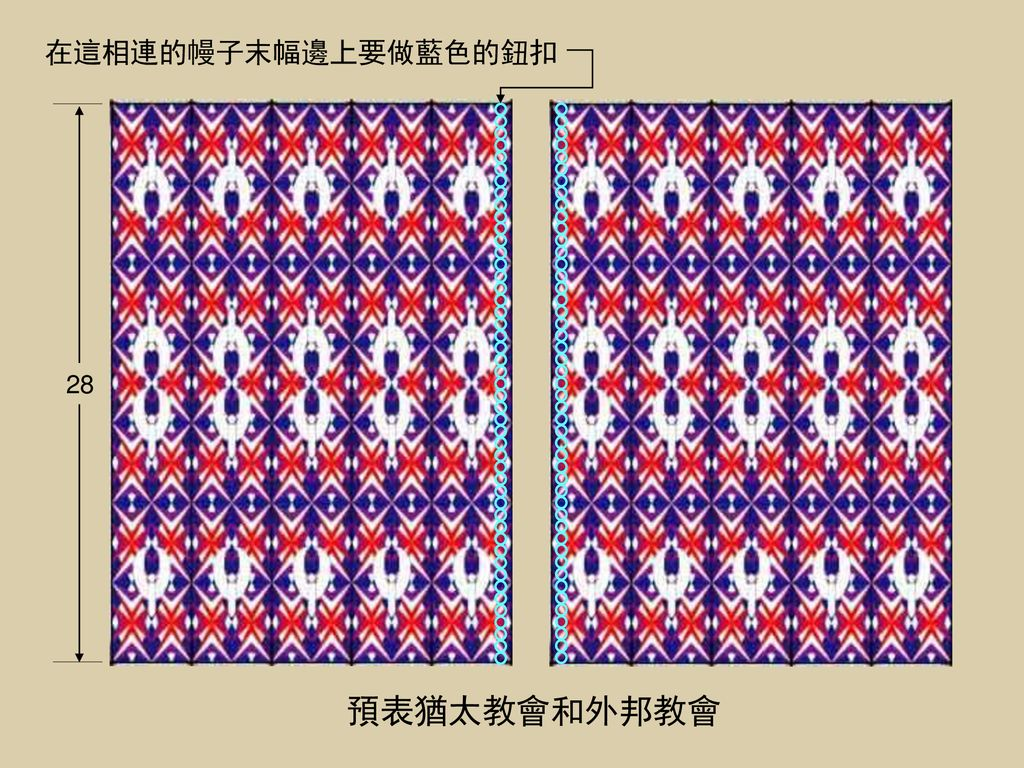
\includegraphics[width=.8\linewidth]{AMoXiFigs/chuaiji/zhangmu12}
 % \caption{A subfigure}
  \label{fig:sub1}
\end{subfigure}%
\begin{subfigure}{.5\textwidth}
  \centering
  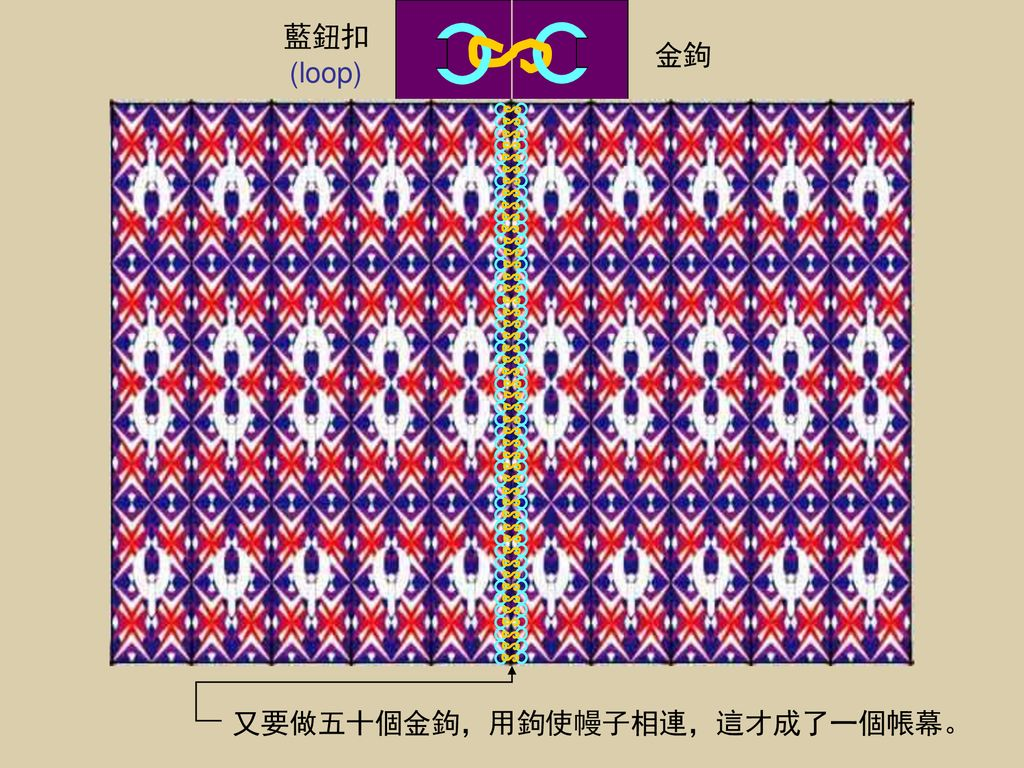
\includegraphics[width=.8\linewidth]{AMoXiFigs/chuaiji/zhangmu1}
%  \caption{A subfigure}
  \label{fig:sub2}
\end{subfigure}
\caption{幕板}
\label{fig:test}
\end{figure}

\begin{figure}[ht]
\centering
\begin{subfigure}{.5\textwidth}
  \centering
  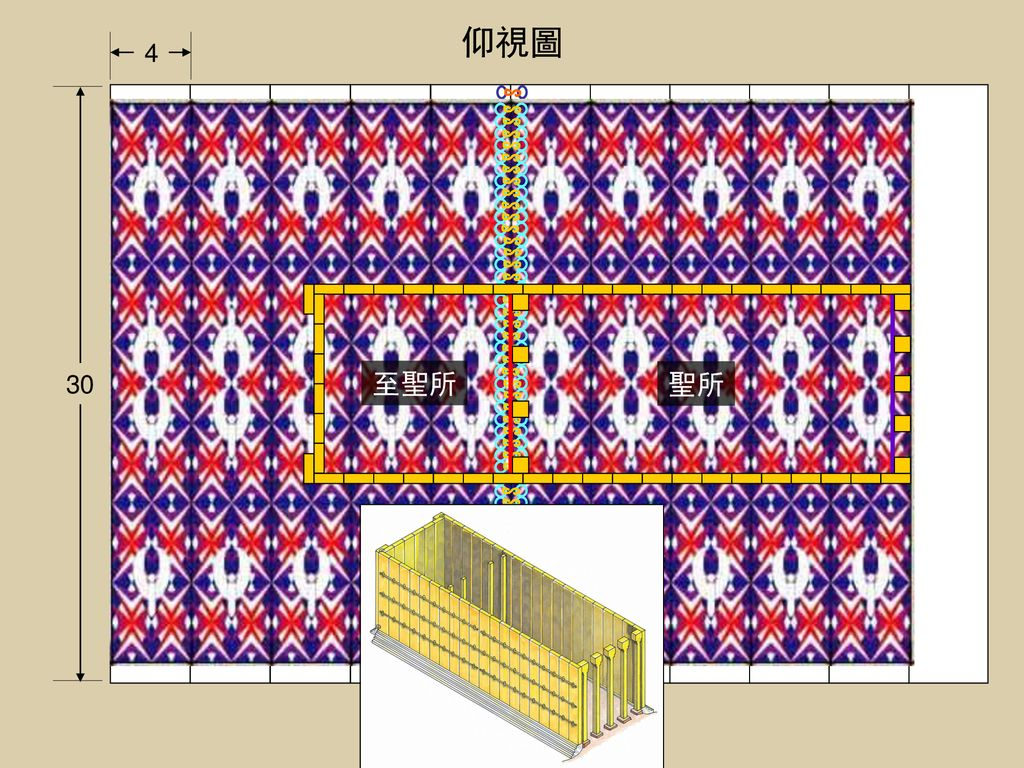
\includegraphics[width=.8\linewidth]{AMoXiFigs/chuaiji/zhangmu4}
 % \caption{A subfigure}
  \label{fig:sub1}
\end{subfigure}%
\begin{subfigure}{.5\textwidth}
  \centering
  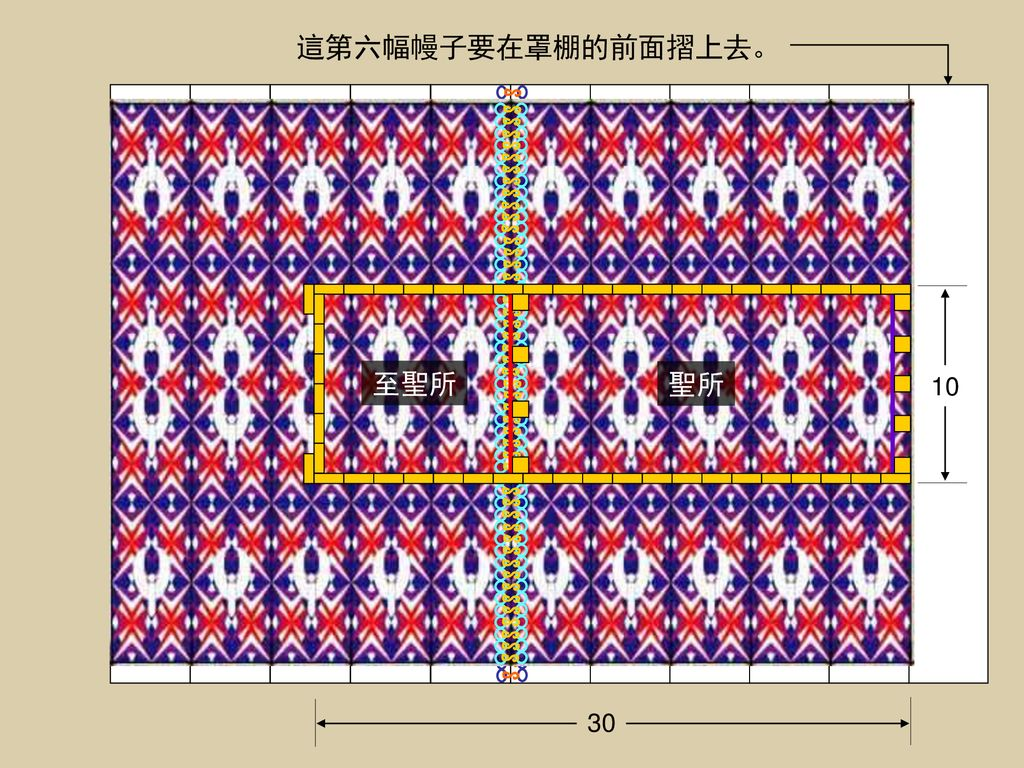
\includegraphics[width=.8\linewidth]{AMoXiFigs/chuaiji/zhangmu6}
%  \caption{A subfigure}
  \label{fig:sub2}
\end{subfigure}
\caption{幕板}
\label{fig:test}
\end{figure}
\begin{figure}[ht]
\centering
\begin{subfigure}{.5\textwidth}
  \centering
  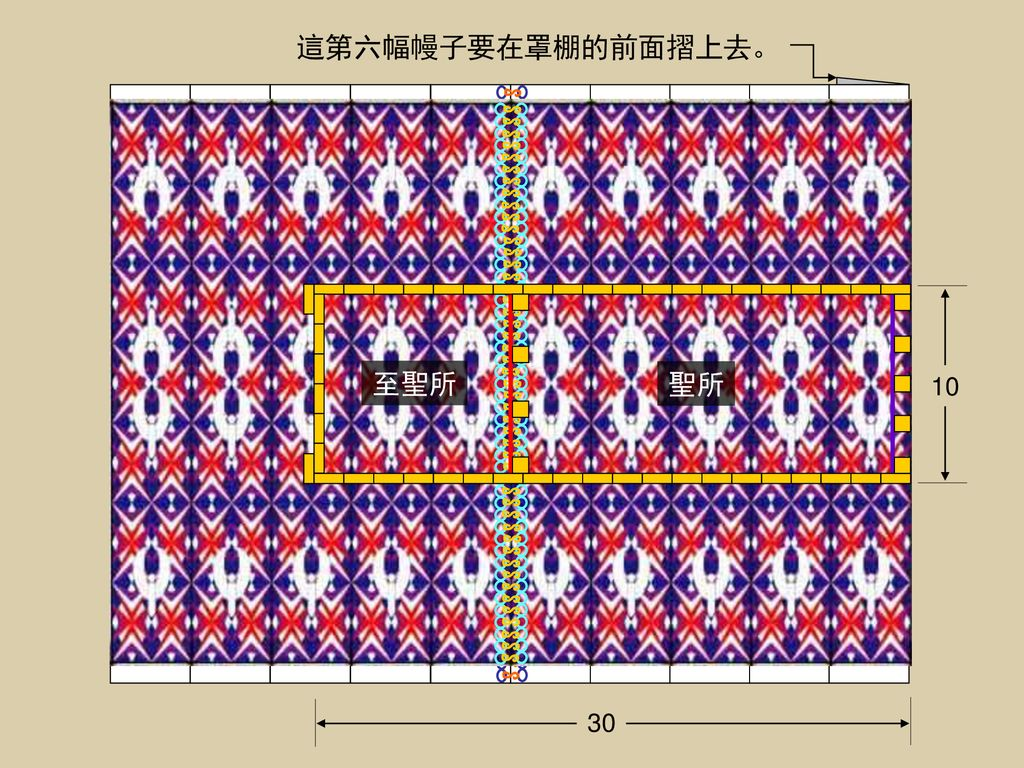
\includegraphics[width=.8\linewidth]{AMoXiFigs/chuaiji/zhangmu7}
 % \caption{A subfigure}
  \label{fig:sub1}
\end{subfigure}%
\begin{subfigure}{.5\textwidth}
  \centering
  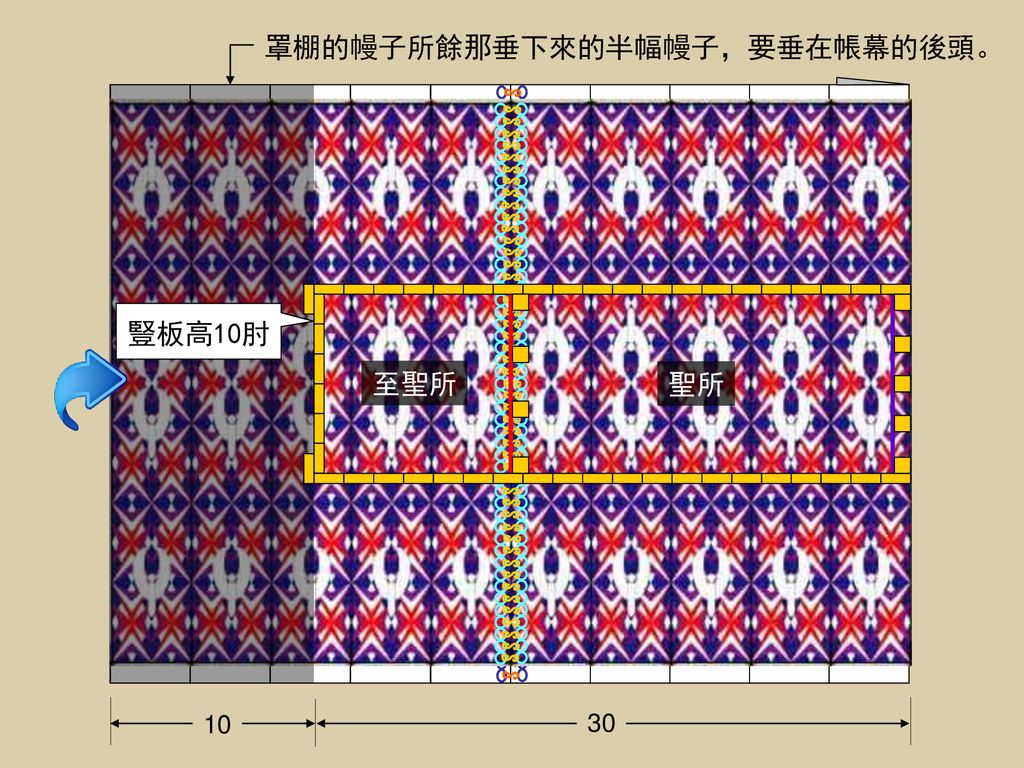
\includegraphics[width=.8\linewidth]{AMoXiFigs/chuaiji/zhangmu8}
%  \caption{A subfigure}
  \label{fig:sub2}
\end{subfigure}
\caption{幕板}
\label{fig:test}
\end{figure}
\begin{figure}[ht]
\centering
\begin{subfigure}{.5\textwidth}
  \centering
  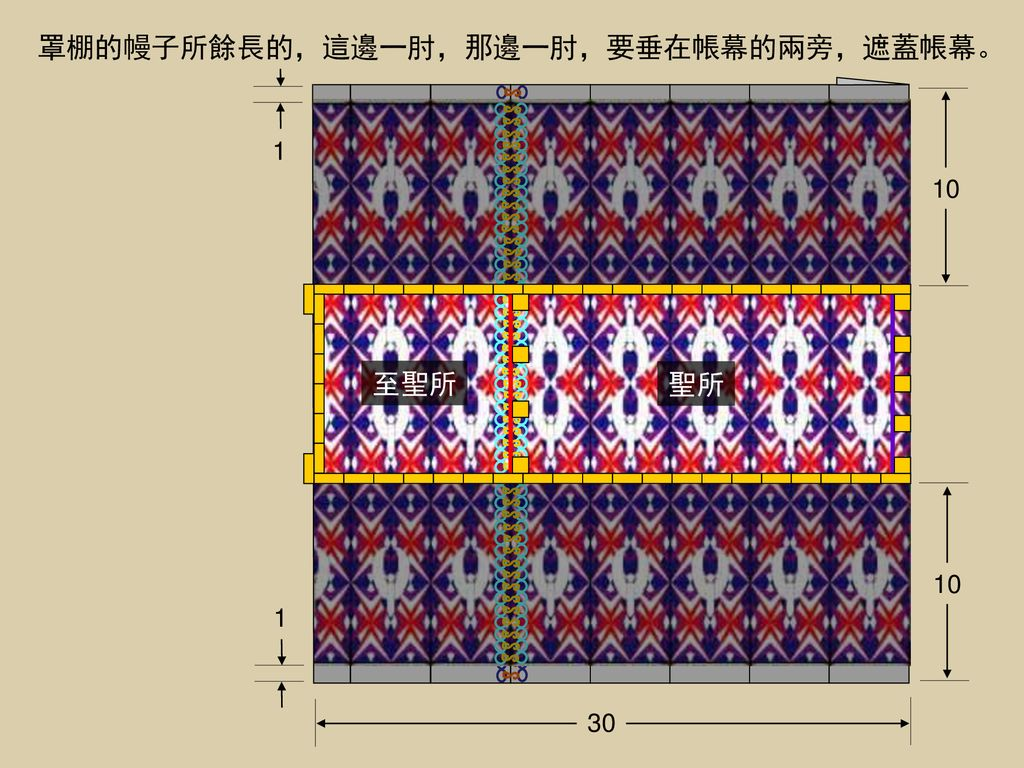
\includegraphics[width=.8\linewidth]{AMoXiFigs/chuaiji/zhangmu9}
 % \caption{A subfigure}
  \label{fig:sub1}
\end{subfigure}%
\begin{subfigure}{.5\textwidth}
  \centering
  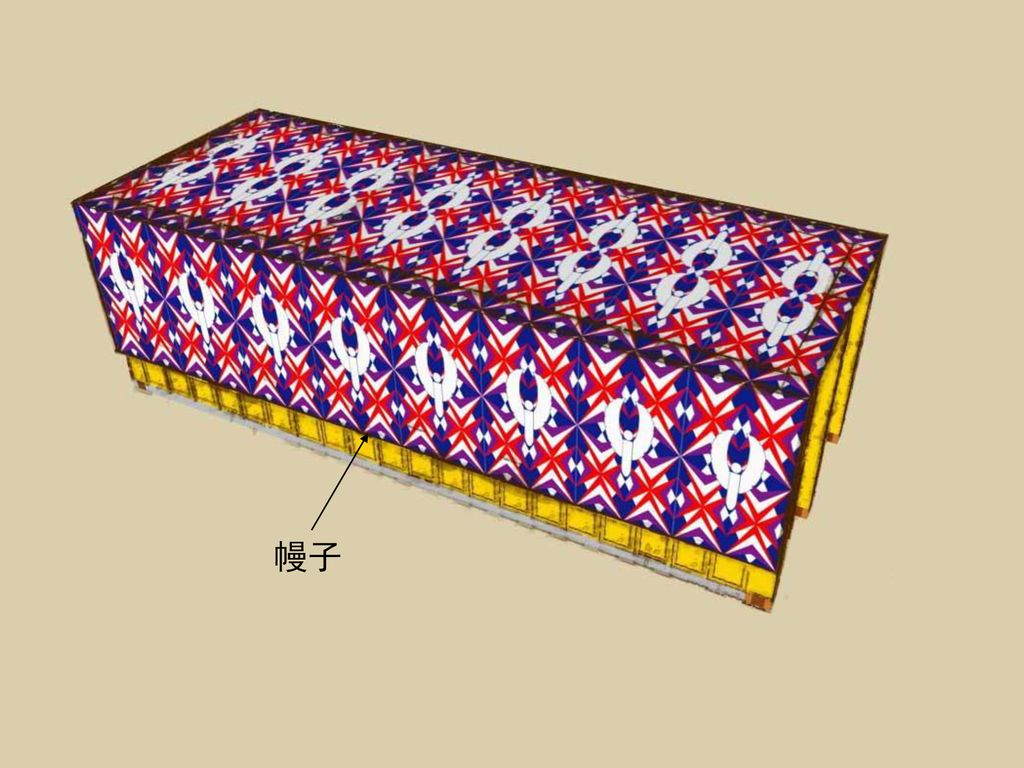
\includegraphics[width=.8\linewidth]{AMoXiFigs/chuaiji/zhangmu11}
%  \caption{A subfigure}
  \label{fig:sub2}
\end{subfigure}
\caption{幕板}
\label{fig:test}
\end{figure}



\subsubsection{造會幕的罩篷 36:14-19}
\begin{figure}[ht]
\centering
\begin{subfigure}{.5\textwidth}
  \centering
  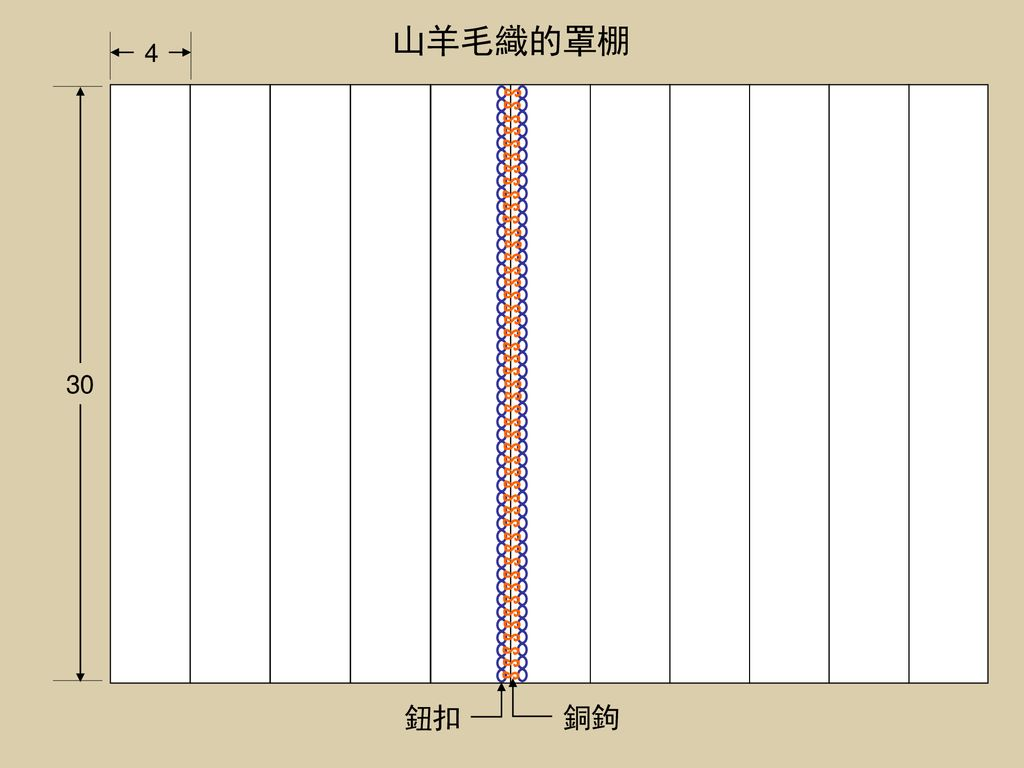
\includegraphics[width=.8\linewidth]{AMoXiFigs/chuaiji/woolcover2}
 % \caption{A subfigure}
  \label{fig:sub1}
\end{subfigure}%
\begin{subfigure}{.5\textwidth}
  \centering
  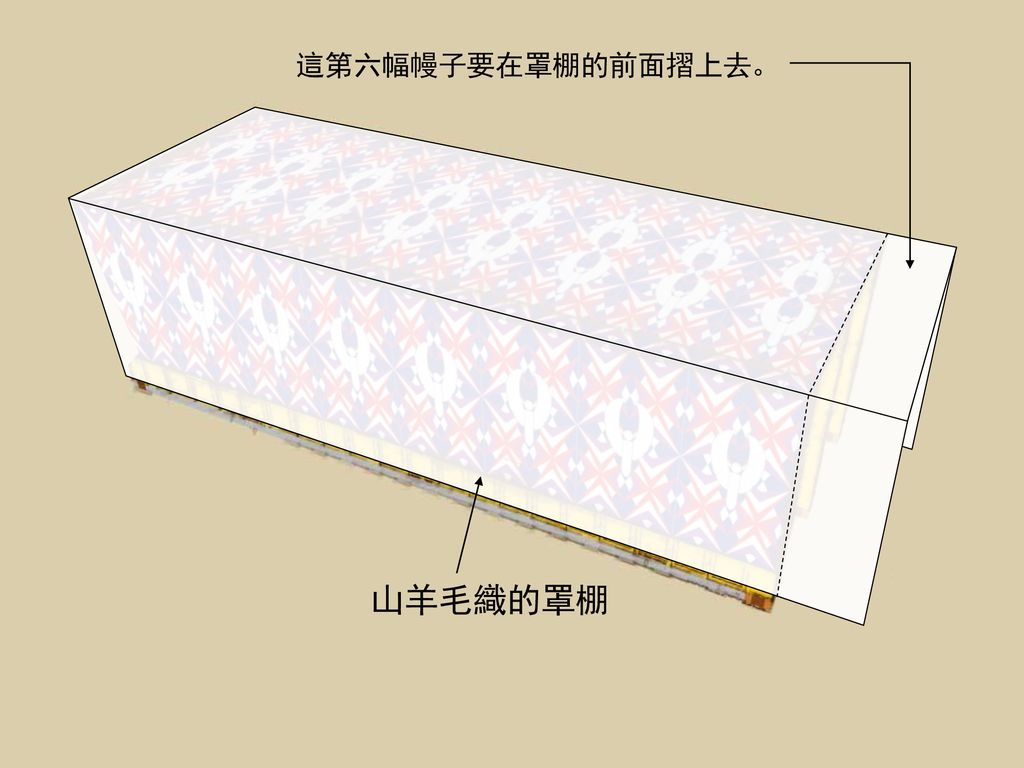
\includegraphics[width=.8\linewidth]{AMoXiFigs/chuaiji/woolcover13}
%  \caption{A subfigure}
  \label{fig:sub2}
\end{subfigure}
\caption{會幕的罩篷}
\label{fig:test}
\end{figure}

\begin{figure}[ht]
\centering
\begin{subfigure}{.5\textwidth}
  \centering
  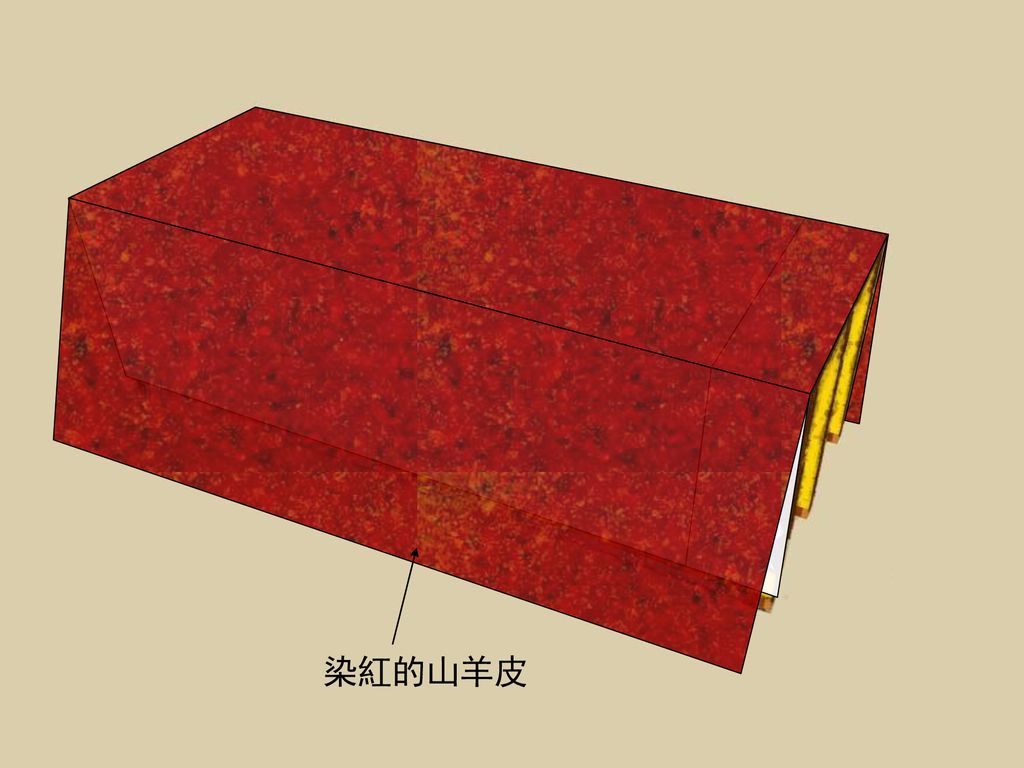
\includegraphics[width=.8\linewidth]{AMoXiFigs/chuaiji/woolcover15}
 % \caption{A subfigure}
  \label{fig:sub1}
\end{subfigure}%
\begin{subfigure}{.5\textwidth}
  \centering
  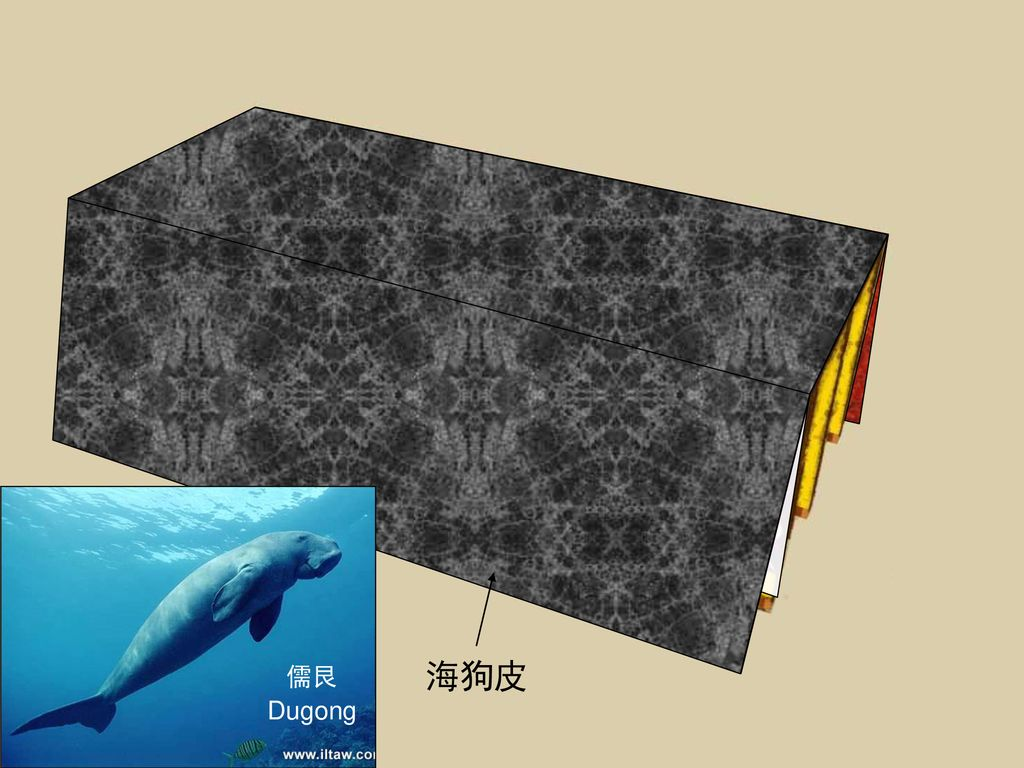
\includegraphics[width=.8\linewidth]{AMoXiFigs/chuaiji/woolcover16}
%  \caption{A subfigure}
  \label{fig:sub2}
\end{subfigure}
\caption{會幕的罩篷}
\label{fig:test}
\end{figure}

\begin{wrapfigure}{r}{0.3\textwidth}
  \centering
  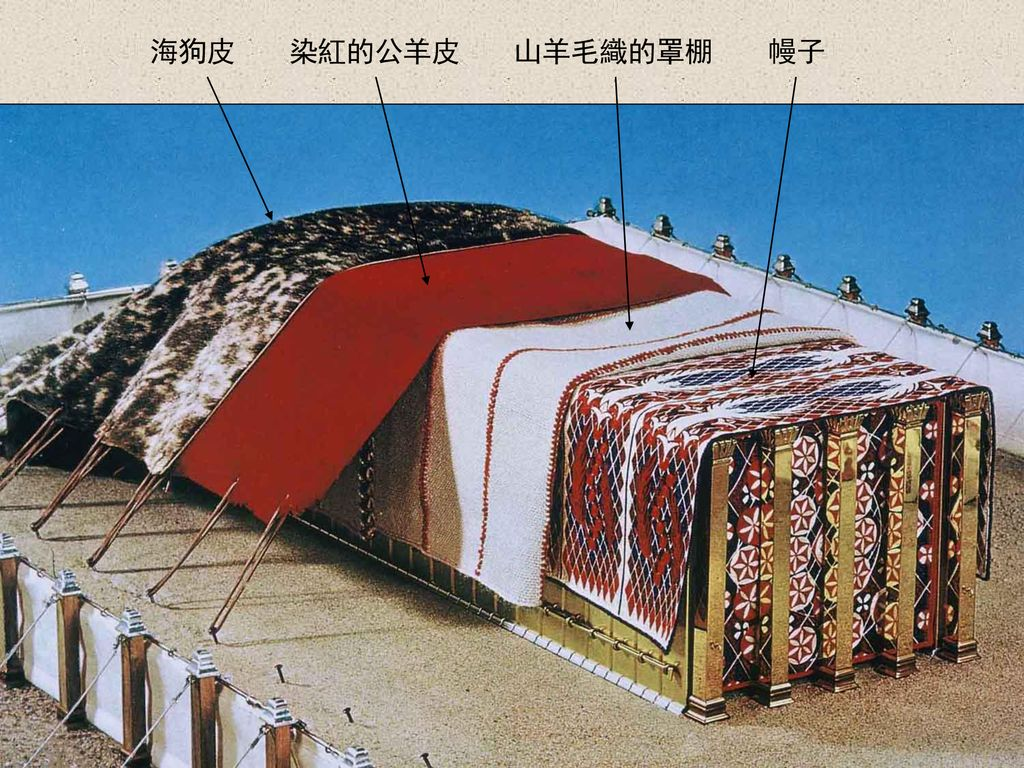
\includegraphics[width=.6\linewidth]{AMoXiFigs/chuaiji/woolcover17}
  \label{fig:sub2}
\caption{會幕的罩篷}
\label{fig:test}
\end{wrapfigure}
他用山羊毛織十一幅幔子，作為帳幕以上的罩篷。每幅幔子長三十肘，寬四肘，十一幅幔子都是一樣的尺寸。 他把五幅幔子連成一幅，又把六幅幔子連成一幅。在這相連的幔子末幅邊上做五十個紐扣，在那相連的幔子末幅邊上也做五十個紐扣。又做五十個銅鉤，使罩篷連成一個。並用染紅的公羊皮做罩篷的蓋，再用海狗皮做一層罩篷上的頂蓋。

\subsubsection{造帳幕的豎板和帶卯的銀座 36:20-34}
\begin{figure}[ht]
\centering
\hspace*{-25mm}
\begin{subfigure}{.33\textwidth}
  \centering
  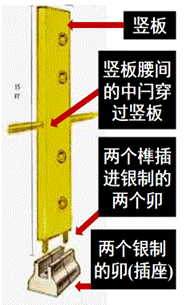
\includegraphics[width=.5\linewidth]{AMoXiFigs/chuaiji/shuban}
 % \caption{A subfigure}
  \label{fig:sub1}
\end{subfigure}%
%\hspace*{ 5mm}
\begin{subfigure}{.33\textwidth}
  \centering
  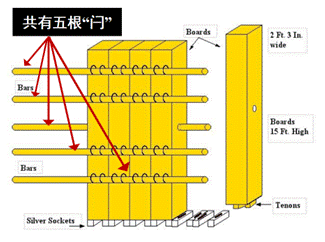
\includegraphics[width=1\linewidth]{AMoXiFigs/chuaiji/shuban1}
%  \caption{A subfigure}
  \label{fig:sub2}
\end{subfigure}
\hspace*{9mm}
\begin{subfigure}{.33\textwidth}
  \centering
  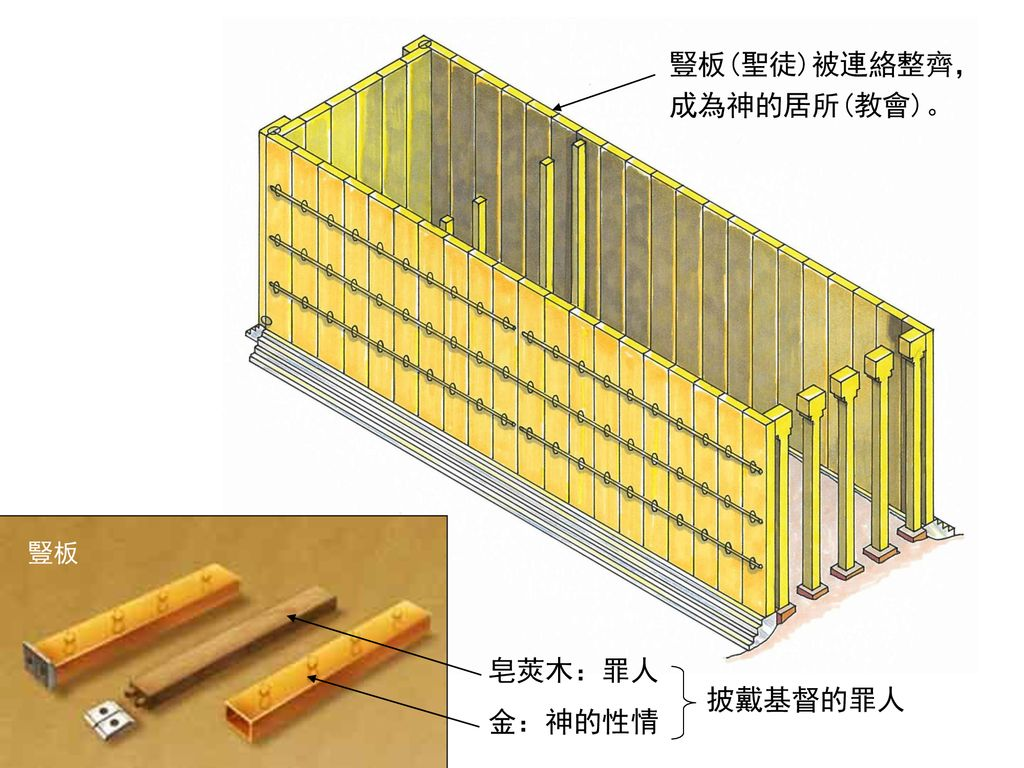
\includegraphics[width=1\linewidth]{AMoXiFigs/chuaiji/shuban2}
%  \caption{A subfigure}
  \label{fig:sub2}
\end{subfigure}
\caption{帳幕的豎板}
\label{fig:test}
\end{figure}


\begin{figure}[ht]
\centering
\begin{subfigure}{.4\textwidth}
  \centering
  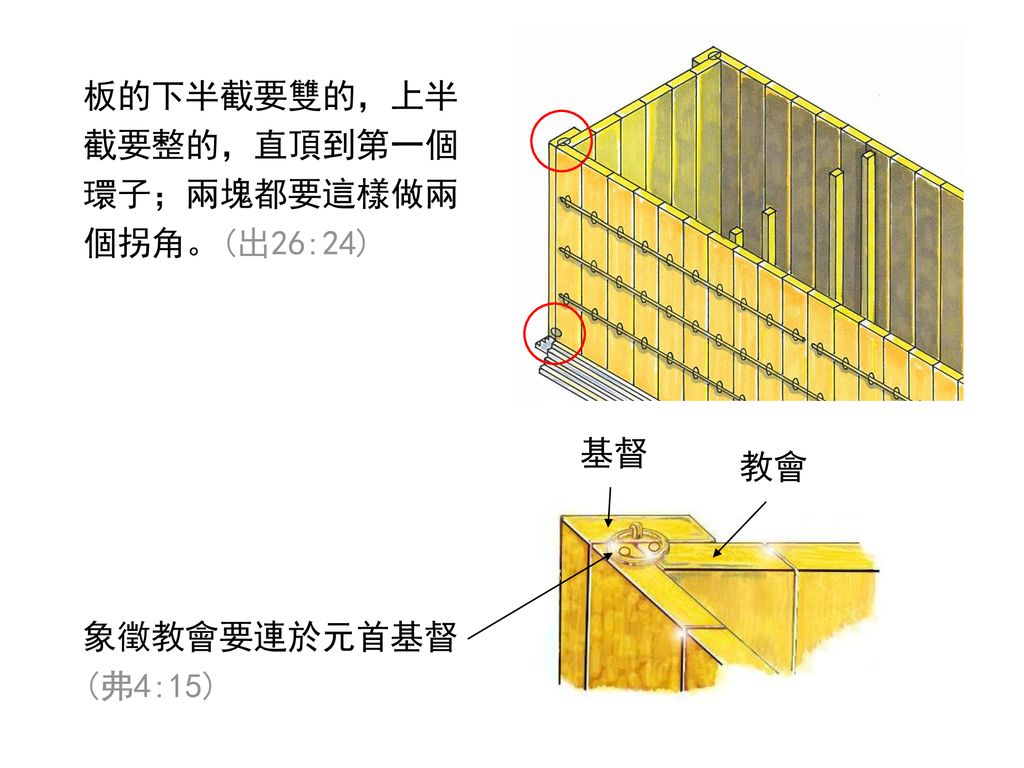
\includegraphics[width=.9\linewidth]{AMoXiFigs/chuaiji/mao}
 % \caption{A subfigure}
  \label{fig:sub1}
\end{subfigure}%
\hspace*{-20mm}
\begin{subfigure}{.4\textwidth}
  \centering
  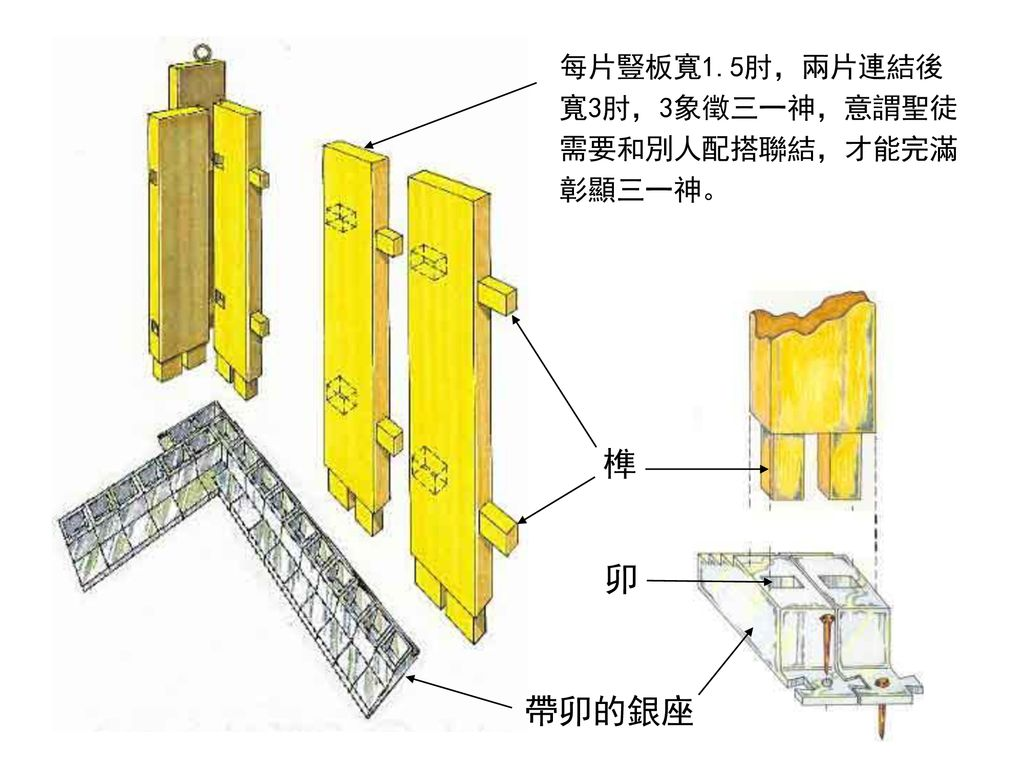
\includegraphics[width=.9\linewidth]{AMoXiFigs/chuaiji/mao3}
%  \caption{A subfigure}
  \label{fig:sub2}
\end{subfigure}
\hspace*{-20mm}
\begin{subfigure}{.4\textwidth}
  \centering
  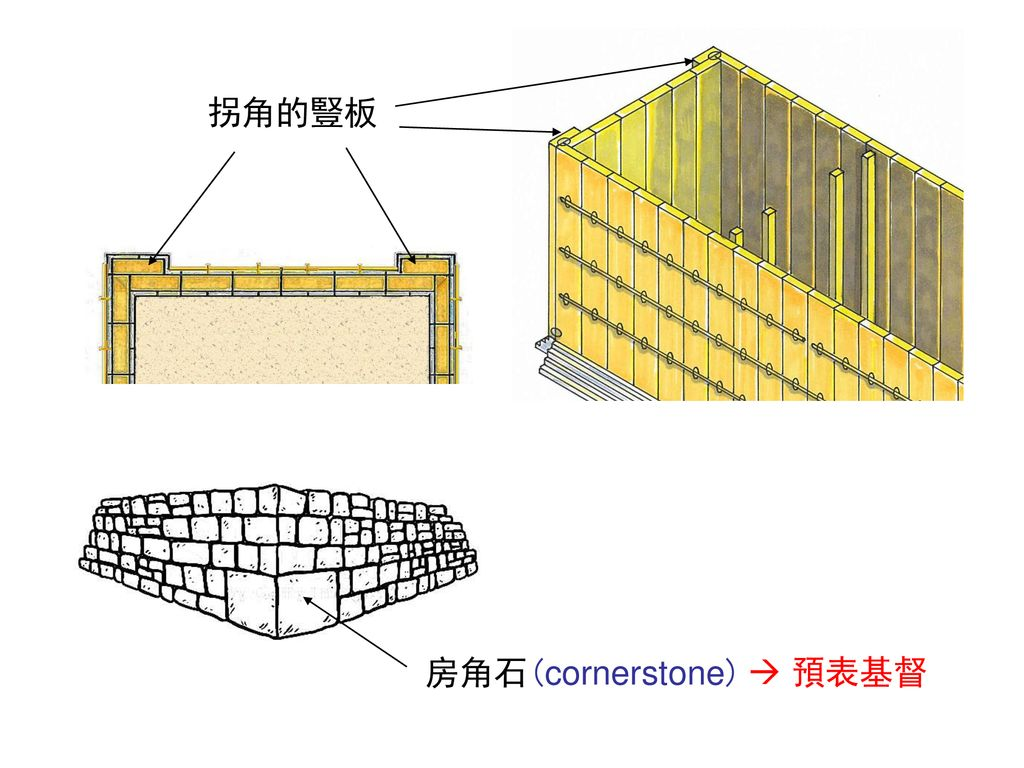
\includegraphics[width=.9\linewidth]{AMoXiFigs/chuaiji/mao5}
%  \caption{A subfigure}
  \label{fig:sub2}
\end{subfigure}
\caption{拐角的豎板}
\label{fig:test}
\end{figure}
他用皂莢木做帳幕的豎板。每塊長十肘，寬一肘半，每塊有兩榫相對。帳幕一切的板都是這樣做。帳幕的南面做板二十塊，在這二十塊板底下又做四十個帶卯的銀座，兩卯接這塊板上的兩榫，兩卯接那塊板上的兩榫。帳幕的第二面，就是北面，也做板二十塊，和帶卯的銀座四十個，這板底下有兩卯，那板底下也有兩卯。帳幕的後面，就是西面，做板六塊。\\
帳幕後面的拐角做板兩塊，板的下半截是雙的，上半截是整的，直到第一個環子，在帳幕的兩個拐角上都是這樣做。有八塊板和十六個帶卯的銀座，每塊板底下有兩卯。他用皂莢木做閂，為帳幕這面的板做五閂， 為帳幕那面的板做五閂，又為帳幕後面的板做五閂，使板腰間的中閂從這一頭通到那一頭。用金子將板包裹，又做板上的金環套閂，閂也用金子包裹。

\subsubsection{造簾 36:35-38}
\begin{wrapfigure}{r}{0.35\textwidth}
\vspace*{-17mm}
%\vspace*{-\baselineskip}
\hspace*{-25mm}
\begin{subfigure}{.5\textwidth}
  \centering
  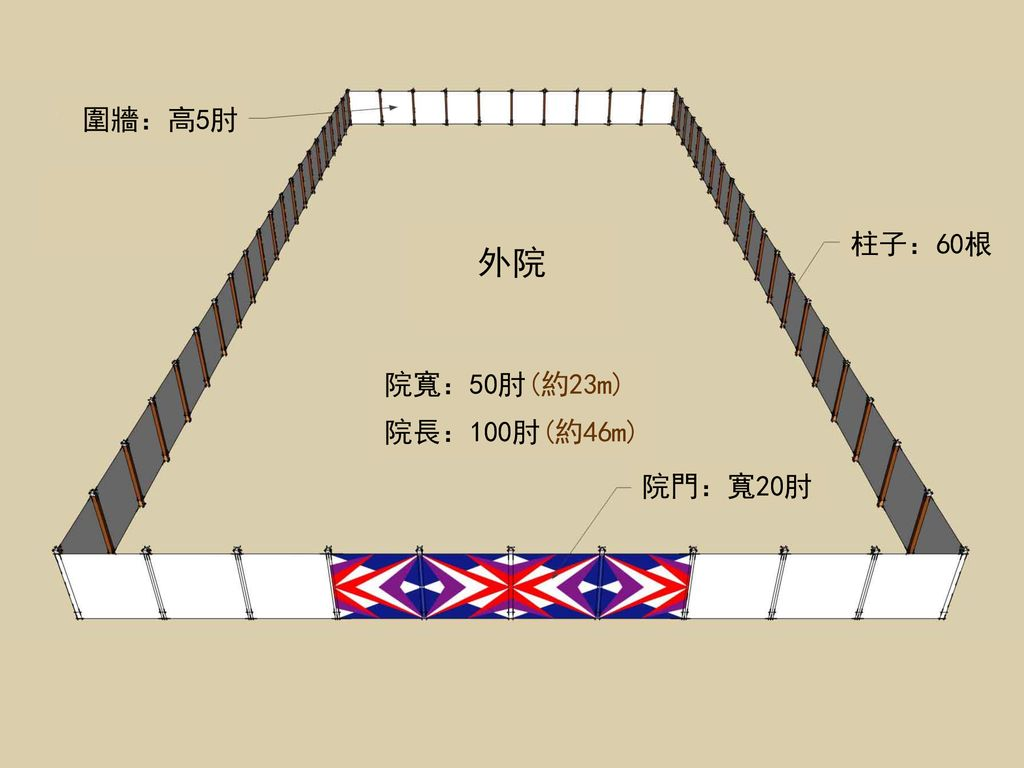
\includegraphics[width=.3\linewidth]{AMoXiFigs/chuaiji/waiyuan}
 % \caption{A subfigure}
  \label{fig:sub1}
\end{subfigure}%
\hspace*{-55mm}
\begin{subfigure}{.5\textwidth}
  \centering
   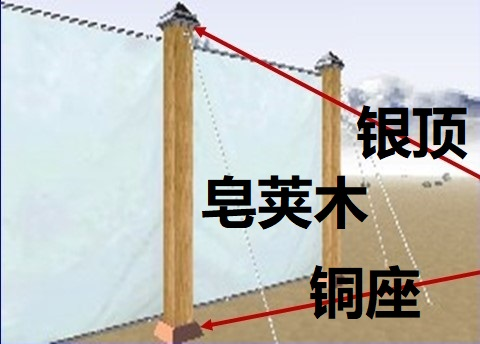
\includegraphics[width=0.32\textwidth]{AMoXiFigs/chuaiji/zhuzi1}
%  \caption{A subfigure}
  \label{fig:sub2}
\end{subfigure}

 % \begin{center}
 %   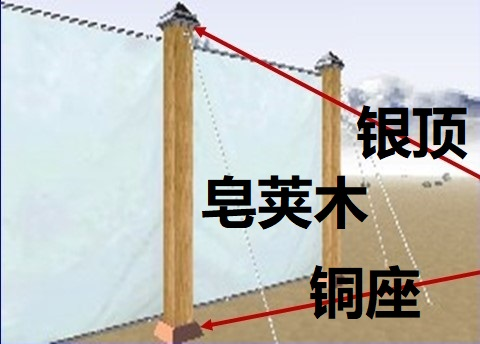
\includegraphics[width=0.16\textwidth]{AMoXiFigs/chuaiji/zhuzi1}
 % \end{center}
%\vspace*{-\baselineskip}
  \caption{簾子}
\end{wrapfigure}
他用藍色、紫色、朱紅色線和撚的細麻織幔子，以巧匠的手工繡上基路伯。為幔子做四根皂莢木柱子，用金包裹，柱子上有金鉤，又為柱子鑄了四個帶卯的銀座。拿藍色、紫色、朱紅色線和撚的細麻，用繡花的手工織帳幕的門簾，又為簾子做五根柱子和柱子上的鉤子，用金子把柱頂和柱子上的杆子包裹。柱子有五個帶卯的座，是銅的。

\subsubsection{造法櫃 37:1-9}
\begin{wrapfigure}{r}{0.35\textwidth}
\vspace*{-17mm}
\hspace*{0mm}
  \centering
  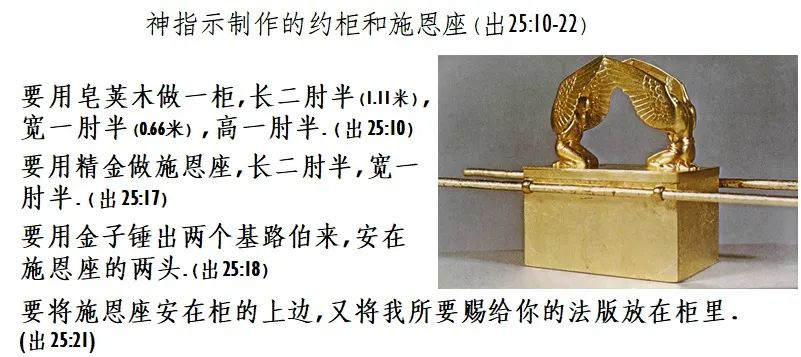
\includegraphics[width=1\linewidth]{AMoXiFigs/chuaiji/yuegui}
  \label{fig:sub1}
\vspace*{-5mm}
  \caption{法櫃 }
\end{wrapfigure}
比撒列用皂莢木做櫃，長二肘半，寬一肘半，高一肘半，裡外包上精金，四圍鑲上金牙邊。又鑄四個金環，安在櫃的四腳上，這邊兩環，那邊兩環。用皂莢木做兩根槓，用金包裹。把槓穿在櫃旁的環內，以便抬櫃。用精金做施恩座，長二肘半，寬一肘半。用金子錘出兩個基路伯來，安在施恩座的兩頭，這頭做一個基路伯，那頭做一個基路伯，二基路伯接連一塊，在施恩座的兩頭。二基路伯高張翅膀，遮掩施恩座，基路伯是臉對臉，朝著施恩座。

\subsubsection{造桌 37:10-16}
他用皂莢木做一張桌子，長二肘，寬一肘，高一肘半，又包上精金，四圍鑲上金牙邊。桌子的四圍各做一掌寬的橫梁，橫梁上鑲著金牙邊。又鑄了四個金環，安在桌子四腳的四角上。安環子的地方是挨近橫梁，可以穿槓抬桌子。他用皂莢木做兩根槓，用金包裹，以便抬桌子。又用精金做桌子上的器皿，就是盤子，調羹，並奠酒的瓶和爵。

\subsubsection{造燈臺 37:17-24}
\begin{wrapfigure}{r}{0.18\textwidth}
\vspace*{-10mm}
%\vspace*{-\baselineskip}
  \begin{center}
    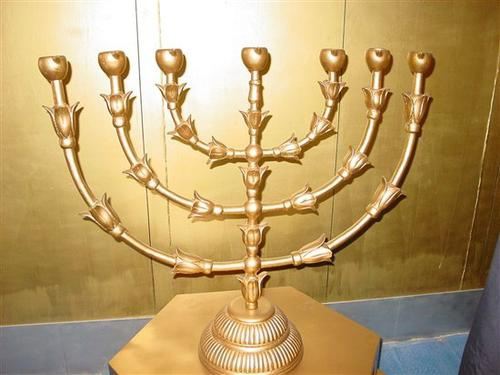
\includegraphics[width=0.18\textwidth]{AMoXiFigs/chuaiji/jindengtai}
  \end{center}
\vspace*{-2mm}
  \caption{燈臺}
\end{wrapfigure}
他用精金做一個燈臺，這燈臺的座和幹與杯、球、花，都是接連一塊錘出來的。燈臺兩旁杈出六個枝子，這旁三個，那旁三個。這旁每枝上有三個杯，形狀像杏花，有球有花；那旁每枝上也有三個杯，形狀像杏花，有球有花。從燈臺杈出來的六個枝子都是如此。 燈臺上有四個杯，形狀像杏花，有球有花。燈臺每兩個枝子以下有球，與枝子接連一塊，燈臺杈出的六個枝子都是如此。球和枝子是接連一塊，都是一塊精金錘出來的。用精金做燈臺的七個燈盞，並燈臺的蠟剪和蠟花盤。他用精金一他連得做燈臺和燈臺的一切器具。

\subsubsection{造香壇 37:25-29}
他用皂莢木做香壇，是四方的，長一肘，寬一肘，高二肘，壇的四角與壇接連一塊。又用精金把壇的上面與壇的四面並壇的四角包裹，又在壇的四圍鑲上金牙邊。做兩個金環，安在牙子邊以下，在壇的兩旁兩根橫撐上，作為穿槓的用處，以便抬壇。用皂莢木做槓，用金包裹。又按做香之法做聖膏油和馨香料的淨香。

\subsubsection{造祭壇 38:1-7}
\begin{wrapfigure}{r}{0.7\textwidth}
\vspace*{-5mm}
%\begin{figure}[ht]
\centering
\begin{subfigure}{.5\textwidth}
  \centering
  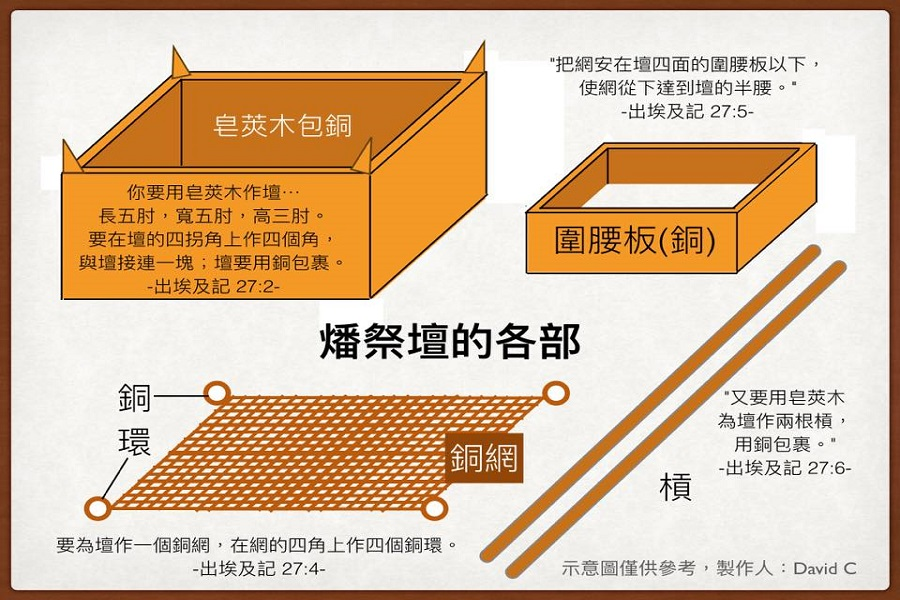
\includegraphics[width=.7\linewidth]{AMoXiFigs/chuaiji/jitan}
 % \caption{A subfigure}
  \label{fig:sub1}
\end{subfigure}%
\hspace*{-30mm}
\begin{subfigure}{.5\textwidth}
  \centering
  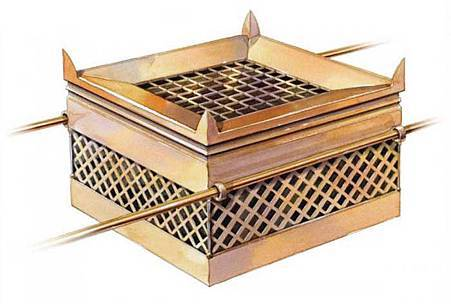
\includegraphics[width=.6\linewidth]{AMoXiFigs/chuaiji/jitan3}
%  \caption{A subfigure}
  \label{fig:sub2}
\end{subfigure}
\caption{祭壇}
\label{fig:test}
\end{wrapfigure}
他用皂莢木做燔祭壇，是四方的，長五肘，寬五肘，高三肘。在壇的四拐角上做四個角，與壇接連一塊，用銅把壇包裹。他做壇上的盆、鏟子、盤子、肉叉子、火鼎，這一切器具都是用銅做的。又為壇做一個銅網，安在壇四面的圍腰板以下，從下達到壇的半腰。為銅網的四角鑄四個環子，作為穿槓的用處。 用皂莢木做槓，用銅包裹，把槓穿在壇兩旁的環子內，用以抬壇；並用板做壇，壇是空的。

\subsubsection{造浴盆 38:8}
他用銅做洗濯盆和盆座，是用會幕門前伺候的婦人之鏡子做的。

\subsubsection{立幕院 38:9-20}

他做帳幕的院子。院子的南面用撚的細麻做帷子，寬一百肘。帷子的柱子二十根，帶卯的銅座二十個，柱子上的鉤子和杆子都是用銀子做的。北面也有帷子，寬一百肘。帷子的柱子二十根，帶卯的銅座二十個，柱子上的鉤子和杆子都是用銀子做的。院子的西面有帷子，寬五十肘。帷子的柱子十根，帶卯的座十個，柱子的鉤子和杆子都是用銀子做的。院子的東面，寬五十肘。門這邊的帷子十五肘，那邊也是一樣。帷子的柱子三根，帶卯的座三個。在門的左右各有帷子十五肘，帷子的柱子三根，帶卯的座三個。院子四面的帷子都是用撚的細麻做的。柱子帶卯的座是銅的，柱子上的鉤子和杆子是銀的，柱頂是用銀子包的。院子一切的柱子都是用銀杆連絡的。院子的門簾是以繡花的手工，用藍色、紫色、朱紅色線和撚的細麻織的，寬二十肘，高五肘，與院子的帷子相配。帷子的柱子四根，帶卯的銅座四個，柱子上的鉤子和杆子是銀的，柱頂是用銀子包的。帳幕一切的橛子和院子四圍的橛子都是銅的。

\subsubsection{核記民獻金銀銅之數 38:21-31}

這是法櫃的帳幕中利未人所用物件的總數，是照摩西的吩咐，經祭司亞倫的兒子以他瑪的手數點的。凡耶和華所吩咐摩西的，都是猶大支派戶珥的孫子、烏利的兒子比撒列做的。與他同工的有但支派中亞希撒抹的兒子亞何利亞伯，他是雕刻匠，又是巧匠，又能用藍色、紫色、朱紅色線和細麻繡花。

\begin{wraptable}{r}{14.5cm}
%\begin{table}[H]
\vspace*{-\baselineskip}
\center
\begin{tabular}{ c c l }
\toprule
材料 &重量 &用途\\\hline
所獻的金子&29他連得730舍客勒 &  \\\hline
被數人所出的銀子&100他連得 &100帶卯的座,1他連得/帶卯的座\\
0.5舍客勒/被數人 &1775舍客勒&做柱子上的鉤子，包裹柱頂並柱子上的杆子\\\hline
銅 &70他連得2400舍客勒&會幕門帶卯的座,銅壇並壇上的銅網並一切器具\\
   &                               &院子四圍,院門帶卯的座,帳幕和院子四圍的橛子\\\hline
\end{tabular}
\caption{技工比撒列,亞何利亞伯}
%\end{table} 
\end{wraptable}
為聖所一切工作使用所獻的\textcolor{blue}{金子}，按聖所的平，有二十九他連得並七百三十舍客勒。會中被數的人所出的\textcolor{blue}{銀子}，按聖所的平，有一百他連得並一千七百七十五舍客勒。凡過去歸那些被數之人的，從二十歲以外，有六十萬零三千五百五十人，按聖所的平，每人出銀半舍客勒，就是一比加。用那一百他連得銀子鑄造聖所帶卯的座和幔子柱子帶卯的座，一百他連得共一百帶卯的座，每帶卯的座用一他連得。用那一千七百七十五舍客勒銀子做柱子上的鉤子，包裹柱頂並柱子上的杆子。所獻的\textcolor{blue}{銅}有七十他連得並二千四百舍客勒。 用這銅做會幕門帶卯的座和銅壇，並壇上的銅網和壇的一切器具，並院子四圍帶卯的座和院門帶卯的座，與帳幕一切的橛子和院子四圍所有的橛子。

\subsubsection{造會幕所用的金屬 39:1-7}
比撒列用藍色、紫色、朱紅色線做精緻的衣服，在聖所用以供職，又為亞倫做聖衣，是照耶和華所吩咐摩西的。他用金線和藍色、紫色、朱紅色線並撚的細麻做以弗得。把金子錘成薄片，剪出線來，與藍色、紫色、朱紅色線，用巧匠的手工一同繡上。又為以弗得做兩條相連的肩帶，接連在以弗得的兩頭。其上巧工織的帶子和以弗得一樣的做法，用以束上，與以弗得接連一塊，是用金線和藍色、紫色、朱紅色線並撚的細麻做的，是照耶和華所吩咐摩西的。
又琢出兩塊紅瑪瑙，鑲在金槽上，彷彿刻圖書，按著以色列兒子的名字雕刻，將這兩塊寶石安在以弗得的兩條肩帶上，為以色列人做紀念石，是照耶和華所吩咐摩西的。

\subsubsection{做胸牌 39:8-21}
他用巧匠的手工做胸牌，和以弗得一樣的做法，用金線與藍色、紫色、朱紅色線並撚的細麻做的。胸牌是四方的，疊為兩層，這兩層長一虎口，寬一虎口，上面鑲著寶石四行：第一行是紅寶石、紅璧璽、紅玉， 第二行是綠寶石、藍寶石、金鋼石，第三行是紫瑪瑙、白瑪瑙、紫晶，第四行是水蒼玉、紅瑪瑙、碧玉。這都鑲在金槽中。 14 這些寶石都是按著以色列十二個兒子的名字，彷彿刻圖書，刻十二個支派的名字。在胸牌上，用精金擰成如繩子的鏈子。又做兩個金槽和兩個金環，安在胸牌的兩頭。 把那兩條擰成的金鏈子穿過胸牌兩頭的環子，又把鏈子的那兩頭接在兩槽上，安在以弗得前面肩帶上。做兩個金環，安在胸牌的兩頭，在以弗得裡面的邊上。 又做兩個金環，安在以弗得前面兩條肩帶的下邊，挨近相接之處，在以弗得巧工織的帶子以上。用一條藍細帶子把胸牌的環子和以弗得的環子繫住，使胸牌貼在以弗得巧工織的帶子上，不可與以弗得離縫，是照耶和華所吩咐摩西的。

\subsubsection{做外袍 39:22-26}
他用織工做以弗得的外袍，顏色全是藍的。袍上留一領口，口的周圍織出領邊來，彷彿鎧甲的領口，免得破裂。在袍子底邊上，用藍色、紫色、朱紅色線並撚的細麻做石榴。又用精金做鈴鐺，把鈴鐺釘在袍子周圍底邊上的石榴中間：一個鈴鐺，一個石榴，一個鈴鐺，一個石榴，在袍子周圍底邊上，用以供職，是照耶和華所吩咐摩西的。

\subsubsection{做內袍 39:27-29}
他用織成的細麻布為亞倫和他的兒子做內袍，並用細麻布做冠冕和華美的裹頭巾，用撚的細麻布做褲子，又用藍色、紫色、朱紅色線並撚的細麻，以繡花的手工做腰帶，是照耶和華所吩咐摩西的。

\subsubsection{造冕牌 39:30-31}
他用精金做聖冠上的牌，在上面按刻圖書之法，刻著：歸耶和華為聖。又用一條藍細帶子將牌繫在冠冕上，是照耶和華所吩咐摩西的。

%\subsection{造會幕竣工 36:8-39:31}
\subsubsection{幕工告竣 39:32-43}
帳幕，就是會幕，一切的工就這樣做完了。凡耶和華所吩咐摩西的，以色列人都照樣做了。他們送到摩西那裡，帳幕和帳幕的一切器具，就是鉤子、板、閂、柱子、帶卯的座，染紅公羊皮的蓋、海狗皮的頂蓋和遮掩櫃的幔子，法櫃和櫃的槓並施恩座，桌子和桌子的一切器具並陳設餅， 精金的燈臺和擺列的燈盞與燈臺的一切器具並點燈的油， 金壇，膏油，馨香的香料，會幕的門簾，銅壇和壇上的銅網，壇的槓並壇的一切器具，洗濯盆和盆座，院子的帷子和柱子，並帶卯的座，院子的門簾、繩子、橛子，並帳幕和會幕中一切使用的器具，精工做的禮服和祭司亞倫並他兒子在聖所用以供祭司職分的聖衣。這一切工作都是以色列人照耶和華所吩咐摩西做的。耶和華怎樣吩咐的，他們就怎樣做了。摩西看見一切的工都做成了，就給他們祝福


\subsubsection{命摩西建會幕 40:1-16}
耶和華曉諭摩西說： 「正月初一日，你要立起帳幕，把法櫃安放在裡面，用幔子將櫃遮掩。把桌子搬進去，擺設上面的物。把燈臺搬進去，點其上的燈。把燒香的金壇安在法櫃前，掛上帳幕的門簾。把燔祭壇安在帳幕門前。把洗濯盆安在會幕和壇的中間，在盆裡盛水。又在四圍立院帷，把院子的門簾掛上。 用膏油把帳幕和其中所有的都抹上，使帳幕和一切器具成聖，就都成聖。又要抹燔祭壇和一切器具，使壇成聖，就都成為至聖。要抹洗濯盆和盆座，使盆成聖。要使亞倫和他兒子到會幕門口來，用水洗身。要給亞倫穿上聖衣，又膏他，使他成聖，可以給我供祭司的職分。又要使他兒子來，給他們穿上內袍。怎樣膏他們的父親，也要照樣膏他們，使他們給我供祭司的職分。他們世世代代凡受膏的，就永遠當祭司的職任。」摩西這樣行，都是照耶和華所吩咐他的。


\subsubsection{會幕完工 40:17-33 }
第二年正月初一日，帳幕就立起來。摩西立起帳幕，安上帶卯的座，立上板，穿上閂，立起柱子，在帳幕以上搭罩篷，把罩篷的頂蓋蓋在其上，是照耶和華所吩咐他的。又把法版放在櫃裡，把槓穿在櫃的兩旁，把施恩座安在櫃上。把櫃抬進帳幕，掛上遮掩櫃的幔子，把法櫃遮掩了，是照耶和華所吩咐他的。又把桌子安在會幕內，在帳幕北邊，在幔子外，在桌子上將餅陳設在耶和華面前，是照耶和華所吩咐他的。又把燈臺安在會幕內，在帳幕南邊，與桌子相對，在耶和華面前點燈，是照耶和華所吩咐他的。把金壇安在會幕內的幔子前，在壇上燒了馨香料做的香，是照耶和華所吩咐他的。又掛上帳幕的門簾。在會幕的帳幕門前，安設燔祭壇，把燔祭和素祭獻在其上，是照耶和華所吩咐他的。把洗濯盆安在會幕和壇的中間，盆中盛水，以便洗濯。摩西和亞倫並亞倫的兒子在這盆裡洗手洗腳。他們進會幕或就近壇的時候，便都洗濯，是照耶和華所吩咐他的。在帳幕和壇的四圍立了院帷，把院子的門簾掛上。這樣，摩西就完了工。

\subsubsection{神的榮光在會幕顯現 40:34-38 （民9:15-23 ）}
當時，雲彩遮蓋會幕，耶和華的榮光就充滿了帳幕。摩西不能進會幕，因為雲彩停在其上，並且耶和華的榮光充滿了帳幕。每逢雲彩從帳幕收上去，以色列人就起程前往；雲彩若不收上去，他們就不起程，直等到雲彩收上去。日間，耶和華的雲彩是在帳幕以上；夜間，雲中有火，在以色列全家的眼前。在他們所行的路上，都是這樣。




















\include{AMoXiFiles/LiWeiJi}
\chapter{民數記}

\section{在西乃的末期 1-10}

\subsection{數點以色列人，各支派依序安營 1:1－2:31}
\subsubsection{核以色列族能臨陣男丁之總數 1:1-3}
以色列人出埃及地後，第二年二月初一日，耶和華在西奈的曠野，會幕中曉諭摩西說：「你要按以色列全會眾的家室、宗族，人名的數目，計算所有的男丁。凡以色列中，從二十歲以外，能出去打仗的，你和亞倫要照他們的軍隊數點。

\subsubsection{派定各族族長 1:4-19}
每支派中，必有一人做本支派的族長，幫助你們。他們的名字：屬\textcolor{blue}{魯本}的，有示丟珥的兒子以利蓿；屬\textcolor{blue}{西緬}的，有蘇利沙代的兒子示路蔑；屬\textcolor{blue}{猶大}的，有亞米拿達的兒子拿順；屬\textcolor{blue}{以薩迦}的，有蘇押的兒子拿坦業；屬\textcolor{blue}{西布倫}的，有希倫的兒子以利押；\textcolor{blue}{約瑟}子孫屬\textcolor{blue}{以法蓮}的，有亞米忽的兒子以利沙瑪；屬\textcolor{blue}{瑪拿西}的，有比大蓿的兒子迦瑪列；屬\textcolor{blue}{便雅憫}的，有基多尼的兒子亞比但；屬\textcolor{blue}{但}的，有亞米沙代的兒子亞希以謝； 屬\textcolor{blue}{亞設}的，有俄蘭的兒子帕結；屬\textcolor{blue}{迦得}的，有丟珥的兒子以利雅薩；屬\textcolor{blue}{拿弗他利}的，有以南的兒子亞希拉。這都是從會中選召的，各做本支派的首領，都是以色列軍中的統領。」於是摩西、亞倫帶著這些按名指定的人，當二月初一日招聚全會眾。會眾就照他們的家室、宗族，人名的數目，從二十歲以外的，都述說自己的家譜。耶和華怎樣吩咐摩西，他就怎樣在西奈的曠野數點他們。

\subsubsection{以色列族被统计的男丁總數 1:20-46}
\begin{wraptable}{r}{10.cm}
\vspace*{-8mm}
\centering
\begin{tabular}{c|c|c|c|c|c}\hline\hline
支派  & 首領名字&  父親名字 &第一次&第二次 &增减\\\hline
流便  &以利蓿 & 示丟珥&46,500 & &\\
西緬  & 示路蔑 &  蘇利沙代&59,300 & & \\
猶大 & 拿順 &亞米拿達&74,600 & &\\
以薩迦 &拿坦業  & 蘇押&54,400 & & \\
西布倫&  以利押& 希倫&57,400 & & \\
以法蓮  &以利沙瑪 & 亞米忽&40,500 & &\\
瑪拿西  & 迦瑪列 &  比大蓿&32,200 & & \\
便雅憫 &亞比但 &基多尼&35,400 && \\
但  &亞希以謝 & 亞米沙代&62,700 && \\
亞設  & 帕結 &  俄蘭&41,500 & & \\
迦得&以利雅薩 & 丟珥&45,650 & & \\
拿弗他利&亞希拉 & 以南&53,400 & & \\\hline
總數&&&603,550&&\\\hline
\end{tabular}
\caption{以色列族被统计的男丁總數}
\end{wraptable}
以色列的長子魯本子孫的後代，照著家室、宗族，人名的數目，從二十歲以外，凡能出去打仗，被數的男丁共有四萬六千五百名。西緬子孫的後代，照著家室、宗族，人名的數目，從二十歲以外，凡能出去打仗，被數的男丁共有五萬九千三百名。迦得子孫的後代，照著家室、宗族，人名的數目，從二十歲以外，凡能出去打仗，被數的共有四萬五千六百五十名。猶大子孫的後代，照著家室、宗族，人名的數目，從二十歲以外，凡能出去打仗，被數的共有七萬四千六百名。以薩迦子孫的後代，照著家室、宗族，人名的數目，從二十歲以外，凡能出去打仗，被數的共有五萬四千四百名。西布倫子孫的後代，照著家室、宗族，人名的數目，從二十歲以外，凡能出去打仗，被數的共有五萬七千四百名。約瑟子孫，屬以法蓮子孫的後代，照著家室、宗族，人名的數目，從二十歲以外，凡能出去打仗，被數的共有四萬零五百名。 瑪拿西子孫的後代，照著家室、宗族，人名的數目，從二十歲以外，凡能出去打仗，被數的共有三萬二千二百名。便雅憫子孫的後代，照著家室、宗族，人名的數目，從二十歲以外，凡能出去打仗，被數的共有三萬五千四百名。但子孫的後代，照著家室、宗族，人名的數目，從二十歲以外，凡能出去打仗，被數的共有六萬二千七百名。亞設子孫的後代，照著家室、宗族，人名的數目，從二十歲以外，凡能出去打仗，被數的共有四萬一千五百名。拿弗他利子孫的後代，照著家室、宗族，人名的數目，從二十歲以外，凡能出去打仗，被數的共有五萬三千四百名。這些就是被數點的，是摩西、亞倫和以色列中十二個首領所數點的，這十二個人各做各宗族的代表。這樣，凡以色列人中被數的，照著宗族從二十歲以外，能出去打仗，被數的共有六十萬零三千五百五十名。

\subsubsection{利未支派不列其數 1:47-54}
利未人卻沒有按著支派數在其中， 48 因為耶和華曉諭摩西說： 49 「唯獨利未支派你不可數點，也不可在以色列人中計算他們的總數。 50 只要派利未人管法櫃的帳幕和其中的器具，並屬乎帳幕的。他們要抬(搬運)帳幕和其中的器具，並要辦理帳幕的事，在帳幕的四圍安營。 51 帳幕將往前行的時候，利未人要拆卸；將支搭的時候，利未人要豎起。近前來的外人必被治死。 52 以色列人支搭帳篷，要照他們的軍隊，各歸本營，各歸本纛。 53 但利未人要在法櫃帳幕的四圍安營，免得憤怒臨到以色列會眾。利未人並要謹守法櫃的帳幕。」 54 以色列人就這樣行。凡耶和華所吩咐摩西的，他們就照樣行了。


\subsubsection{東邊支派首領及安營之所 2:1-8}
\begin{wrapfigure}{r}{0.5\textwidth}
\vspace*{-22mm}
\begin{center} 
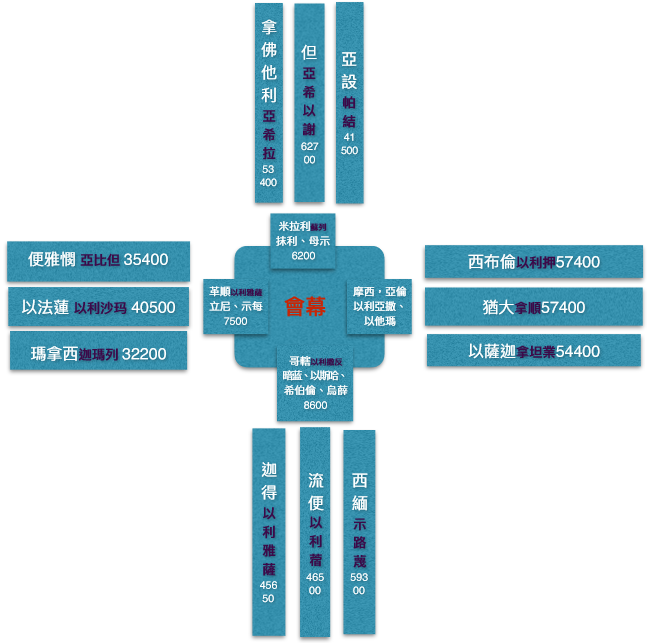
\includegraphics[width=0.85\textwidth]{AMoXiFigs/fig1}
\caption{各支派族長，人數及位置}
\label{fig:1} 
\end{center}
\end{wrapfigure}
耶和華曉諭摩西、亞倫說：「以色列人要各歸自己的纛下，在本族的旗號那裡，對著會幕的四圍安營。在\textcolor{red}{東邊}向日出之地，照著軍隊安營的是猶大營的纛。有亞米拿達的兒子拿順做猶大人的首領， 4 他軍隊被數的，共有七萬四千六百名； 5 挨著他安營的是以薩迦支派，有蘇押的兒子拿坦業做以薩迦人的首領， 6 他軍隊被數的，共有五萬四千四百名； 7 又有西布倫支派，希倫的兒子以利押做西布倫人的首領， 8 他軍隊被數的，共有五萬七千四百名。 9 凡屬猶大營，按著軍隊被數的，共有十八萬六千四百名，要做第一隊往前行。

\subsubsection{南邊支派首領及安營之所 2:9-16}
在\textcolor{red}{南邊}，按著軍隊是魯本營的纛。有示丟珥的兒子以利蓿做魯本人的首領， 11 他軍隊被數的，共有四萬六千五百名； 12 挨著他安營的是西緬支派，蘇利沙代的兒子示路蔑做西緬人的首領， 13 他軍隊被數的，共有五萬九千三百名； 14 又有迦得支派，丟珥的兒子以利雅薩做迦得人的首領， 15 他軍隊被數的，共有四萬五千六百五十名。 16 凡屬魯本營，按著軍隊被數的，共有十五萬一千四百五十名，要做第二隊往前行。

\subsubsection{利未營在諸營中間 2:17}
隨後會幕要往前行，有利未營在諸營\textcolor{red}{中間}。他們怎樣安營就怎樣往前行，各按本位，各歸本纛。

\subsubsection{西邊支派首領及安營之所 2:18-24}
在\textcolor{red}{西邊}，按著軍隊是以法蓮營的纛。亞米忽的兒子以利沙瑪做以法蓮人的首領， 19 他軍隊被數的，共有四萬零五百名； 20 挨著他的是瑪拿西支派，比大蓿的兒子迦瑪列做瑪拿西人的首領， 21 他軍隊被數的，共有三萬二千二百名； 22 又有便雅憫支派，基多尼的兒子亞比但做便雅憫人的首領， 23 他軍隊被數的，共有三萬五千四百名。 24 凡屬以法蓮營，按著軍隊被數的，共有十萬零八千一百名，要做第三隊往前行。

\subsubsection{北邊支派首領及安營之所 2:25-31}
在\textcolor{red}{北邊}，按著軍隊是但營的纛。亞米沙代的兒子亞希以謝做但人的首領， 26 他軍隊被數的，共有六萬二千七百名； 27 挨著他安營的是亞設支派，俄蘭的兒子帕結做亞設人的首領， 28 他軍隊被數的，共有四萬一千五百名； 29 又有拿弗他利支派，以南的兒子亞希拉做拿弗他利人的首領， 30 他軍隊被數的，共有五萬三千四百名。 31 凡但營被數的，共有十五萬七千六百名，要歸本纛做末隊往前行。

\subsection{數點利未支派 2:32－4:49}
\subsubsection{唯獨利未人沒有被數 2:32-34}
這些以色列人，照他們的宗族，按他們的軍隊，在諸營中被數的，共有六十萬零三千五百五十名。唯獨利未人沒有數在以色列人中，是照耶和華所吩咐摩西的。以色列人就這樣行，各人照他們的家室、宗族歸於本纛，安營起行，都是照耶和華所吩咐摩西的。

\subsubsection{亞倫和摩西的後代 3:1-4}
\begin{wraptable}{r}{5.cm}
\vspace*{-5mm}
\centering
\begin{tabular}{ c|c|c }\hline\hline
拿答-長子 & 獻凡火而死&受膏祭司\\ 
亞比戶 &獻凡火而死&受膏祭司\\  
以利亞撒 &供祭司職分&受膏祭司   \\
以他瑪  & 供祭司職分&受膏祭司   \\\hline
\end{tabular}
\caption{亞倫後裔}
\end{wraptable}
耶和華在西奈山曉諭摩西的日子，亞倫和摩西的後代如下：亞倫的兒子，長子名叫拿答，還有亞比戶、以利亞撒、以他瑪。這是亞倫兒子的名字，都是受膏的祭司，是摩西叫他們承接聖職供祭司職分的。拿答、亞比戶在西奈的曠野向耶和華獻凡火的時候，就死在耶和華面前了，他們也沒有兒子。以利亞撒、以他瑪在他們的父親亞倫面前供祭司的職分。

\subsubsection{區別利未人服侍亞倫 3:5-10}

耶和華曉諭摩西說：「你使利未支派近前來，站在祭司亞倫面前好服侍他，替他和會眾在會幕前守所吩咐的，辦理帳幕的事。又要看守會幕的器具，並守所吩咐以色列人的，辦理帳幕的事。你要將利未人給亞倫和他的兒子，因為他們是從以色列人中選出來給他的。你要囑咐亞倫和他的兒子謹守自己祭司的職任。近前來的外人必被治死。」

\subsubsection{利未人代替以色列人一切頭生 3:11-13}
耶和華曉諭摩西說： 12 「我從以色列人中揀選了利未人，代替以色列人一切頭生的，利未人要歸我， 13 因為凡頭生的是我的。我在埃及地擊殺一切頭生的那日，就把以色列中一切頭生的，連人帶牲畜都分別為聖歸我，他們定要屬我。我是耶和華。」

\subsubsection{利未宗族的家室 3:14-20}
\begin{figure}[H]
\centering
%\begin{center}
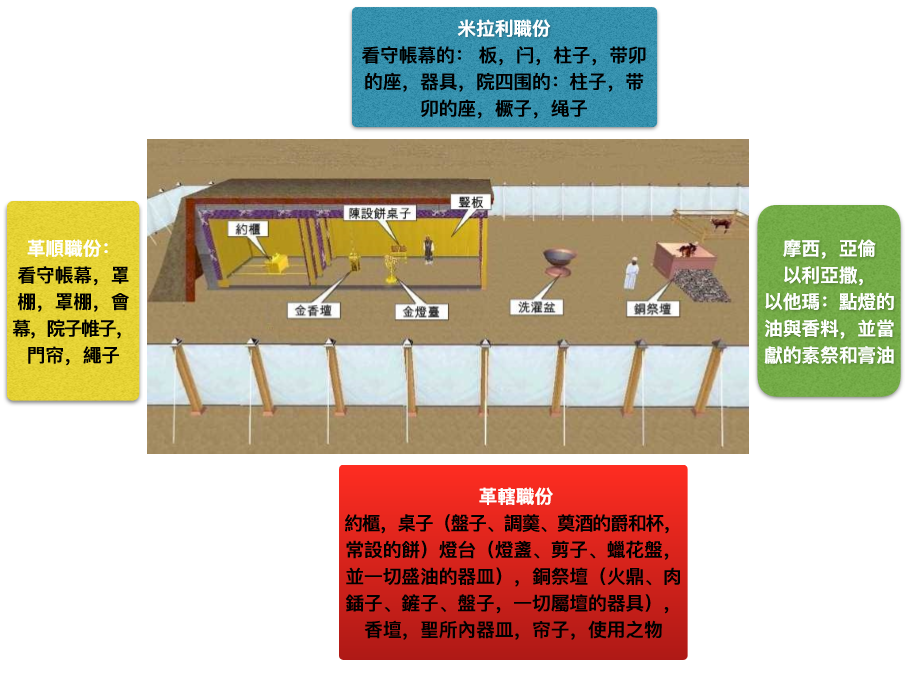
\includegraphics[width=5in]{AMoXiFigs/fig2}
\caption{圖2：利未各支派職分及位置}
\label{fig:1} 
%\end{center}
\end{figure}
耶和華在西奈的曠野曉諭摩西說： 15 「你要照利未人的宗族、家室數點他們，凡一個月以外的男子都要數點。」 16 於是摩西照耶和華所吩咐的，數點他們。 17 利未眾子的名字是革順、哥轄、米拉利。 18 革順的兒子，按著家室，是立尼、示每； 19 哥轄的兒子，按著家室，是暗蘭、以斯哈、希伯倫、烏薛； 20 米拉利的兒子，按著家室，是抹利、母示。這些按著宗族是利未人的家室。

\subsubsection{革順男丁之數及職份 3:21-26}
屬革順的，有立尼族、示每族，這是革順的二族。其中被數，從一個月以外所有的男子，共有七千五百名。這革順的二族要在帳幕後西邊安營。拉伊勒的兒子以利雅薩做革順人宗族的首領。革順的子孫在會幕中所要看守的，就是帳幕和罩篷，並罩篷的蓋與會幕的門簾，院子的帷子和門簾（院子是圍帳幕和壇的），並一切使用的繩子。

\subsubsection{革轄男丁之數及職份 3:27-43}
屬哥轄的，有暗蘭族、以斯哈族、希伯倫族、烏薛族，這是哥轄的諸族。按所有男子的數目，從一個月以外看守聖所的，共有八千六百名。哥轄兒子的諸族要在帳幕的南邊安營。烏薛的兒子以利撒反做哥轄宗族家室的首領。他們所要看守的是約櫃、桌子、燈臺、兩座壇與聖所內使用的器皿，並簾子和一切使用之物。祭司亞倫的兒子以利亞撒做利未人眾首領的領袖，要監察那些看守聖所的人。

\subsubsection{米拉利男丁之數及職份 3:33-37}
屬米拉利的，有瑪利族、母示族，這是米拉利的二族。他們被數的，按所有男子的數目，從一個月以外的，共有六千二百名。亞比亥的兒子蘇列做米拉利二宗族的首領。他們要在帳幕的北邊安營。米拉利子孫的職分是看守帳幕的板、閂、柱子、帶卯的座和帳幕一切所使用的器具，院子四圍的柱子、帶卯的座、橛子和繩子。

\subsubsection{摩西、亞倫和亞倫兒子的職份 3:38}
在帳幕前東邊向日出之地安營的是摩西、亞倫和亞倫的兒子。他們看守聖所，替以色列人守耶和華所吩咐的。近前來的外人必被治死。 

\subsubsection{利未人代替以色列族首生之男 3:39-51}
\begin{table}[H]
\centering
\begin{tabular}{c|c|c|c|c}
\hline
\hline
    &革順  & 革轄  & 米拉利&  總數  \\
\hline
各族     & 立尼，示每 & 暗蘭，以斯哈，希伯倫，烏薛  & 抹利，母示&   \\
\hline
人數（一個月以上）&7500&8600&6200&22000  \\ 
\hline
人數（30-50歲）& 2630 &  2750 &3200&8580  \\
\hline
\end{tabular}
\caption{利未支派}
\end{table}
39 凡被數的利未人，就是摩西、亞倫照耶和華吩咐所數的，按著家室，從一個月以外的男子，共有二萬二千名。

40 耶和華對摩西說：「你要從以色列人中數點一個月以外，凡頭生的男子，把他們的名字記下。 41 我是耶和華。你要揀選利未人歸我，代替以色列人所有頭生的；也取利未人的牲畜，代替以色列所有頭生的牲畜。」 42 摩西就照耶和華所吩咐的，把以色列人頭生的都數點了。 43 按人名的數目，從一個月以外，凡頭生的男子，共有二萬二千二百七十三名。

 耶和華曉諭摩西說：「你揀選利未人代替以色列人所有頭生的，也取利未人的牲畜代替以色列人的牲畜。利未人要歸我。我是耶和華。以色列人中頭生的男子比利未人多二百七十三個，必當將他們贖出來。你要按人丁，照聖所的平，每人取贖銀五舍客勒（一舍客勒是二十季拉），把那多餘之人的贖銀交給亞倫和他的兒子。」於是摩西從那被利未人所贖以外的人取了贖銀。從以色列人頭生的所取之銀，按聖所的平，有一千三百六十五舍客勒。摩西照耶和華的話把這贖銀給亞倫和他的兒子，正如耶和華所吩咐的。

\subsubsection{祭司亞倫和兒子職任 4:1-14}
耶和華曉諭摩西、亞倫說：「你從利未人中，將哥轄子孫的總數，照他們的家室、宗族，從三十歲直到五十歲，凡前來任職，在會幕裡辦事的，全都計算。哥轄子孫在會幕搬運至聖之物，所辦的事乃是這樣：起營的時候，亞倫和他兒子要進去
\begin{itemize} 
\itemsep-.35em
\item 摘下遮掩櫃的幔子，用以蒙蓋\textcolor{blue}{法櫃}。又用海狗皮蓋在上頭，再蒙上純藍色的毯子，把\textcolor{red}{槓}穿上。
\item 又用藍色毯子鋪在\textcolor{blue}{陳設餅的桌子上}，將盤子、調羹、奠酒的爵和杯擺在上頭，桌子上也必有常設的餅。在其上又要蒙朱紅色的毯子，再蒙上海狗皮，把\textcolor{red}{槓}穿上。
\item 要拿藍色毯子，把\textcolor{blue}{燈臺和燈臺上所用的}燈盞、剪子、蠟花盤並一切盛油的器皿，全都遮蓋。又要把燈臺和燈臺的一切器具包在海狗皮裡，放在\textcolor{red}{抬架}上。
\item 在\textcolor{blue}{金壇}上要鋪藍色毯子，蒙上海狗皮，把\textcolor{red}{槓}穿上。
\item 又要把聖所用的\textcolor{blue}{一切器具}包在藍色毯子裡，用海狗皮蒙上，放在\textcolor{red}{抬架}上。
\item 要收去壇上的灰，把紫色毯子鋪在壇上。又要把所用的一切器具，就是火鼎、肉叉子、鏟子、盤子，一切\textcolor{blue}{屬壇的器具}都擺在壇上。又蒙上海狗皮，把\textcolor{red}{槓}穿上。 
\end{itemize}

\subsubsection{哥轄子孫之職任 4:15-20}
將要起營的時候，\textcolor{blue}{亞倫和他兒子}把聖所和聖所的一切器具遮蓋完了，\textcolor{blue}{哥轄的子孫}就要來抬，只是不可摸聖物，免得他們死亡。會幕裡這些物件是哥轄子孫所當抬的。\textcolor{blue}{祭司亞倫的兒子以利亞撒}所要看守的是點燈的油與香料，並當獻的素祭和膏油，也要看守全帳幕與其中所有的，並聖所和聖所的器具。
耶和華曉諭摩西、亞倫說：「你們不可將哥轄人的支派從利未人中剪除。他們挨近至聖物的時候，\textcolor{blue}{亞倫和他兒子}要進去，派他們各人所當辦的、所當抬的。這樣待他們，好使他們活著，不致死亡。只是他們連片時不可進去觀看聖所，免得他們死亡。」

\subsubsection{革順子孫在以他瑪手下之職任 4:21-28}
耶和華曉諭摩西說：「你要將革順子孫的總數，照著宗族、家室，從三十歲直到五十歲，凡前來任職，在會幕裡辦事的，全都數點。革順人各族所辦的事、所抬的物乃是這樣：他們要抬帳幕的\textcolor{blue}{幔子}和會幕，並會幕的\textcolor{blue}{蓋}與其上的\textcolor{blue}{海狗皮}和會幕的\textcolor{blue}{門簾}，院子的\textcolor{blue}{帷子}和\textcolor{blue}{門簾}（院子是圍帳幕和壇的）、\textcolor{blue}{繩子}，並所用的\textcolor{blue}{器具}，不論是做什麼用的，他們都要經理。革順的子孫在一切抬物辦事之上都要憑亞倫和他兒子的吩咐。他們所當抬的，要派他們看守。這是革順子孫的各族在會幕裡所辦的事。他們所看守的，必在祭司亞倫兒子以他瑪的手下。

\subsubsection{米拉利子孫在以他瑪手下之職任 4:29-33}
至於米拉利的子孫，你要照著家室、宗族把他們數點。從三十歲直到五十歲，凡前來任職，在會幕裡辦事的，你都要數點。他們辦理會幕的事，就是抬帳幕的\textcolor{blue}{板、閂、柱子和帶卯的座}，院子四圍的\textcolor{blue}{柱子}和其上\textcolor{blue}{帶卯的座}，\textcolor{blue}{橛子}、\textcolor{blue}{繩子}，並\textcolor{blue}{一切使用的器具}。他們所抬的器具，你們要按名指定。這是米拉利子孫各族在會幕裡所辦的事，都在祭司亞倫兒子以他瑪的手下。

\subsubsection{記利未人自三十歲至五十歲者之數 4:34-49}
摩西、亞倫與會眾的諸首領將\textcolor{blue}{哥轄的子孫}，照著家室、宗族，從三十歲直到五十歲，凡前來任職，在會幕裡辦事的，都數點了，被數的共有二千七百五十名。這是哥轄各族中被數的，是在會幕裡辦事的，就是摩西、亞倫照耶和華藉摩西所吩咐數點的。
\textcolor{blue}{革順子孫}被數的，照著家室、宗族，從三十歲直到五十歲，凡前來任職，在會幕裡辦事的，共有二千六百三十名。這是革順子孫各族中被數的，是在會幕裡辦事的，就是摩西、亞倫照耶和華藉摩西所吩咐數點的。
\textcolor{blue}{米拉利子孫}中各族被數的，照著家室、宗族， 從三十歲直到五十歲，凡前來任職，在會幕裡辦事的，共有三千二百名。 這是米拉利子孫各族中被數的，就是摩西、亞倫照耶和華藉摩西所吩咐數點的。
凡\textcolor{blue}{被數的利未人}，就是摩西、亞倫並以色列眾首領，照著家室、宗族所數點的，從三十歲直到五十歲，凡前來任職，在會幕裡做抬物之工的，共有八千五百八十名。摩西按他們所辦的事、所抬的物，憑耶和華的吩咐數點他們。他們這樣被摩西數點，正如耶和華所吩咐他的。


\subsection{頒布生活，婚姻，生命潔净的律法 5-6}
\subsubsection{不潔者出到營外 5:1-4 }
耶和華曉諭摩西說：「你吩咐以色列人，使一切長大痲瘋的、患漏症的並因死屍不潔淨的，都出營外去。無論男女都要使他們出到營外，免得汙穢他們的營。這營是我所住的。」以色列人就這樣行，使他們出到營外。耶和華怎樣吩咐摩西，以色列人就怎樣行了。

\subsubsection{犯罪的要賠償 5:5-8}
耶和華對摩西說：「你曉諭以色列人說：無論男女，若犯了人所常犯的罪，以致干犯耶和華，那人就有了罪。他要承認所犯的罪，將所虧負人的如數賠還，另外加上五分之一，也歸於所虧負的人。那人若沒有親屬可受所賠還的，那所賠還的就要歸於服侍耶和華的祭司。至於那為他贖罪的公羊是在外。以色列人一切的聖物中，所奉給祭司的舉祭都要歸於祭司。各人所分別為聖的物，無論是什麼，都要歸給祭司。」

\subsubsection{歸給祭司的物 5:9-10}
以色列人一切的聖物中，所奉給祭司的舉祭都要歸於祭司。各人所分別為聖的物，無論是什麼，都要歸給祭司。

\subsubsection{妻子貞節實驗方法 5:11-31}
耶和華對摩西說： 12 「你曉諭以色列人說：人的妻若有邪行，得罪她丈夫， 13 有人與她行淫，事情嚴密，瞞過她丈夫，而且她被玷汙，沒有做見證的人，當她行淫的時候也沒有被捉住， 14 她丈夫生了疑恨的心，疑恨她，她是被玷汙，或是她丈夫生了疑恨的心，疑恨她，她並沒有被玷汙， 15 這人就要將妻送到祭司那裡，又為她帶著大麥麵伊法十分之一做供物，不可澆上油，也不可加上乳香，因為這是疑恨的素祭，是思念的素祭，使人思念罪孽。

祭司要使那婦人近前來，站在耶和華面前。 17 祭司要把聖水盛在瓦器裡，又從帳幕的地上取點塵土，放在水中。 18 祭司要叫那婦人蓬頭散髮，站在耶和華面前，把思念的素祭，就是疑恨的素祭，放在她手中。祭司手裡拿著致咒詛的苦水， 19 要叫婦人起誓，對她說：『若沒有人與你行淫，也未曾背著丈夫做汙穢的事，你就免受這致咒詛苦水的災。 20 你若背著丈夫行了汙穢的事，在你丈夫以外有人與你行淫， 21 （祭司叫婦人發咒起誓）願耶和華叫你大腿消瘦，肚腹發脹，使你在你民中被人咒詛，成了誓語， 22 並且這致咒詛的水入你的腸中，要叫你的肚腹發脹，大腿消瘦。』婦人要回答說：『阿們！阿們！』

祭司要寫這咒詛的話，將所寫的字抹在苦水裡， 24 又叫婦人喝這致咒詛的苦水。這水要進入她裡面變苦了。 25 祭司要從婦人的手中取那疑恨的素祭，在耶和華面前搖一搖，拿到壇前。 26 又要從素祭中取出一把，作為這事的紀念，燒在壇上，然後叫婦人喝這水。 27 叫她喝了以後，她若被玷汙，得罪了丈夫，這致咒詛的水必進入她裡面變苦了，她的肚腹就要發脹，大腿就要消瘦，那婦人便要在她民中被人咒詛； 28 若婦人沒有被玷汙，卻是清潔的，就要免受這災，且要懷孕。

妻子背著丈夫行了汙穢的事， 30 或是人生了疑恨的心，疑恨他的妻，就有這疑恨的條例。那時他要叫婦人站在耶和華面前，祭司要在她身上照這條例而行。 31 男人就為無罪，婦人必擔當自己的罪孽。

\noindent
疑恨（思念）的素祭=大麥麵1/10伊法+無油無乳香\\
1） 過程\\
  祭司要使那婦人近前來，站在耶和華面前發咒起誓；
  婦人要回答說：『阿們，阿們。』
  祭司要寫這咒詛的話，將所寫的字抹在苦水裏，從素祭中取出一把燒在壇上，叫婦人喝這水\\
2）判斷方法 \\
   $\cdot${ 她若被玷污得罪了丈夫，這致咒詛的水必進入她裏面變變苦了，她的肚腹就要發脹，大腿就要消瘦，那婦人便要在他民中被人咒詛。}\\
   $\cdot${ 若婦人沒有被玷污，卻是清潔的，就要免受這災，且要懷孕。}


\subsubsection{拿細耳人的條例 6:1-21}
\subsubsubsection{做拿細耳(歸主)人的要求 6:1-8}
耶和華對摩西說：「你曉諭以色列人說：無論男女許了特別的願，就是拿細耳(歸主)人的願，要離俗歸耶和華，
\vspace*{-2mm}
\begin{itemize} 
\itemsep-.35em
\item 他就要遠離清酒濃酒，也不可喝什麼清酒濃酒做的醋。不可喝什麼葡萄汁，也不可吃鮮葡萄和乾葡萄。在一切離俗的日子，凡葡萄樹上結的，自核至皮所做的物，都不可吃。
\item 在他一切許願離俗的日子，不可用剃頭刀剃頭，要由髮綹長長了。他要聖潔，直到離俗歸耶和華的日子滿了。
\item 在他離俗歸耶和華的一切日子，不可挨近死屍。他的父母或是弟兄姐妹死了的時候，他不可因他們使自己不潔淨，因為那離俗歸神的憑據是在他頭上。在他一切離俗的日子，是歸耶和華為聖。
\end{itemize} 

\subsubsubsection{拿細耳(歸主)人被沾染的要求 6:9-12}
\begin{itemize} 
\itemsep-.35em
\item 若在他旁邊忽然有人死了，以致沾染了他離俗的頭，他要在第七日得潔淨的時候剃頭。第八日，他要把兩隻斑鳩或兩隻雛鴿帶到會幕門口，交給祭司。
\item 祭司要獻一隻做贖罪祭，一隻做燔祭，為他贖那因死屍而有的罪，並要當日使他的頭成為聖潔。
\item 他要另選離俗歸耶和華的日子，又要牽一隻一歲的公羊羔來做贖愆祭；但先前的日子要歸徒然，因為他在離俗之間被玷汙了。
\end{itemize} 

\subsubsubsection{拿細耳(歸主)滿了離俗期的條例 6:13-21}
拿細耳人滿了離俗的日子乃有這條例：
\vspace*{-2mm}
\begin{itemize} 
\itemsep-.35em
\item 人要領他到會幕門口，他要將供物奉給耶和華，就是一隻沒有殘疾、一歲的公羊羔做燔祭，一隻沒有殘疾、一歲的母羊羔做贖罪祭，和一隻沒有殘疾的公綿羊做平安祭，並一筐子無酵調油的細麵餅與抹油的無酵薄餅，並同獻的素祭和奠祭。
\item 祭司要在耶和華面前獻那人的贖罪祭和燔祭，也要把那隻公羊和那筐無酵餅獻給耶和華做平安祭，又要將同獻的素祭和奠祭獻上。
\item 拿細耳人要在會幕門口剃離俗的頭，把離俗頭上的髮放在平安祭下的火上。
\item 他剃了以後，祭司就要取那已煮的公羊一條前腿，又從筐子裡取一個無酵餅和一個無酵薄餅，都放在他手上。祭司要拿這些作為搖祭，在耶和華面前搖一搖，這與所搖的胸、所舉的腿同為聖物，歸給祭司。
\item 然後，拿細耳人可以喝酒。
\end{itemize}
\vspace*{-2mm}
許願的拿細耳人為離俗所獻的供物和他以外所能得的獻給耶和華，就有這條例。他怎樣許願就當照離俗的條例行。

\subsubsection{祭司為以色列人祝福之語 6:22-27}
耶和華曉諭摩西說：「你告訴亞倫和他兒子說，你們要這樣為以色列人祝福，說：
\vspace*{-2mm}
\begin{itemize} 
\itemsep-.35em
\item \textcolor{blue}{願耶和華}賜福給你，保護你！
\item \textcolor{blue}{願耶和華}使他的臉光照你，賜恩給你！
\item \textcolor{blue}{願耶和華}向你仰臉，賜你平安！
\end{itemize} 
\vspace*{-2mm}
他們要如此奉我的名為以色列人祝福，我也要賜福給他們。」


%\subsection{信仰分别为聖各族長向會幕獻祭 7}
\subsection{信仰分别為聖-各族長向會幕獻祭 7:1-89}
\subsubsection{會幕建立族長獻禮 7:1-3}
摩西立完了帳幕，就\textcolor{blue}{把帳幕用膏抹}了，使它\textcolor{red}{成聖}；又把其中的\textcolor{blue}{器具和壇並壇上的器具，都抹}了，使它\textcolor{red}{成聖}。\textcolor{red}{當天}，以色列的眾首領，就是\textcolor{blue}{各族的族長}，都來奉獻。他們是各支派的首領管理那些被數的人。他們把自己的供物送到耶和華面前，就是六輛篷子車和十二隻公牛。每兩個首領奉獻一輛車，每首領奉獻一隻牛。他們把這些都\textcolor{blue}{奉到帳幕前}。

\subsubsection{族長獻禮的分配原则 7:4-10}
\begin{wraptable}{r}{5.cm}
%\vspace*{-5mm}
\centering
\begin{tabular}{|c|c|c|c|}
\hline
\hline
     &革轄 &革順  & 米拉利    \\
\hline
車子 & -   & 兩輛&四輛   \\
\hline
公牛&- &四隻&八隻  \\ 
\hline
\end{tabular}
\caption{眾族長獻禮的分配}
\end{wraptable}
%\vspace*{-4mm}
耶和華曉諭摩西說：「你要收下這些，好做會幕的使用，都要照利未人所辦的事交給他們。」於是摩西收了車和牛，交給利未人，把兩輛車、四隻牛，照\textcolor{blue}{革順子孫}所辦的事交給他們，又把四輛車、八隻牛，照\textcolor{blue}{米拉利子孫}所辦的事交給他們。他們都在祭司亞倫的兒子以他瑪手下。但車與牛都\textcolor{blue}{沒有交給哥轄子孫}，因為他們辦的是聖所的事，在肩頭上抬聖物。用\textcolor{blue}{膏抹壇的日子}，首領都來行奉獻壇的禮，眾首領就在\textcolor{blue}{壇前獻供物}。

\subsubsection{眾族長獻供物及獻禮顺序 7:11-83}

\begin{table}[H]
\centering
\begin{tabular}{|c|c|c|c|c|}
\hline
\hline
 素祭 & 香 & 燔祭 & 贖罪祭 & 平安祭 \\\hline
銀盤子（130舍客勒）&金盂& 公牛（1）&公山羊(1) &公牛（2） \\
銀碗（70舍客勒）     &（10舍客勒）& 公綿羊(1)         &           & 公綿羊（5）/ 公山羊（5）  \\
盛滿調油細麵         &盛滿了香   & 一歲的公羊羔(1) &          &一歲的公羊羔（5）   \\\hline
\end{tabular}
\caption{各首領向會幕獻的祭物}
\end{table}

\begin{table}[H]
\centering
\begin{tabular}{|c|c|c|c|c|}
\hline
\hline
營纛  & 獻祭次序&  支派 &首領名字 &父親名字 \\
\hline
\multirow{3}{*}{猶大營} & 第一日    & \textcolor{red}{猶大} &拿順 &亞米拿達  \\
\cline{2-5}
\multicolumn{1}{|c|}{}  & 第二日  & 以薩迦 &拿坦業  & 蘇押  \\
\cline{2-5}
\multicolumn{1}{|c|}{} & 第三日  & 西布倫&  以利押& 希倫  \\
\cline{2-5}
\hline
\multirow{3}{*}{流便營} &  第四日  &\textcolor{red}{流便}  &以利蓿 & 示丟珥 \\
\cline{2-5}
\multicolumn{1}{|c|}{}  &   第五日 &西緬  & 示路蔑 &  蘇利沙代  \\
\cline{2-5}
\multicolumn{1}{|c|}{} & 第六日  & 迦得&以利雅薩 & 丟珥  \\
\hline
\multirow{3}{*}{以法蓮營} &  第七日  &\textcolor{red}{以法蓮}  &以利沙瑪 & 亞米忽 \\
\cline{2-5}
\multicolumn{1}{|c|}{}  &   第八日 &瑪拿西  & 迦瑪列 &  比大蓿  \\
\cline{2-5}
\multicolumn{1}{|c|}{} & 第九日  & 便雅憫&亞比但 & 基多尼  \\
\hline
\multirow{3}{*}{但營} &  第十日  &\textcolor{red}{但}  &亞希以謝 & 亞米沙代 \\
\cline{2-5}
\multicolumn{1}{|c|}{}  &   第十一日 &亞設  & 帕結 &  俄蘭  \\
\cline{2-5}
\multicolumn{1}{|c|}{} & 第十二日  & 拿弗他利&亞希拉 & 以南  \\
\hline
\end{tabular}
\caption{各族長獻祭次序}
\end{table}


\subsubsubsection{頭一日猶大支派獻禮 7:11-17}
耶和華對摩西說：「眾首領為行奉獻壇的禮，要每天一個首領來獻供物。」頭一日獻供物的是猶大支派的亞米拿達的兒子拿順。他的供物是：一個銀盤子，重一百三十舍客勒，一個銀碗，重七十舍客勒，都是按聖所的平，也都盛滿了調油的細麵做素祭。一個金盂，重十舍客勒，盛滿了香。一隻公牛犢，一隻公綿羊，一隻一歲的公羊羔做燔祭；一隻公山羊做贖罪祭；兩隻公牛，五隻公綿羊，五隻公山羊，五隻一歲的公羊羔做平安祭。這是亞米拿達兒子拿順的供物。

\subsubsubsection{第二日以薩迦支派獻禮 7:18-23}
第二日來獻的是以薩迦子孫的首領，蘇押的兒子拿坦業。他獻為供物的是：一個銀盤子，重一百三十舍客勒，一個銀碗，重七十舍客勒，都是按聖所的平，也都盛滿了調油的細麵做素祭。一個金盂，重十舍客勒，盛滿了香。一隻公牛犢，一隻公綿羊，一隻一歲的公羊羔做燔祭；一隻公山羊做贖罪祭；兩隻公牛，五隻公綿羊，五隻公山羊，五隻一歲的公羊羔做平安祭。這是蘇押兒子拿坦業的供物。

\subsubsubsection{第三日西布倫支派獻禮 7:24-29}
第三日來獻的是西布倫子孫的首領，希倫的兒子以利押。他的供物是：一個銀盤子，重一百三十舍客勒，一個銀碗，重七十舍客勒，都是按聖所的平，也都盛滿了調油的細麵做素祭。一個金盂，重十舍客勒，盛滿了香。 一隻公牛犢，一隻公綿羊，一隻一歲的公羊羔做燔祭； 一隻公山羊做贖罪祭；兩隻公牛，五隻公綿羊，五隻公山羊，五隻一歲的公羊羔做平安祭。這是希倫兒子以利押的供物。

\subsubsubsection{第四日魯本支派獻禮 7:30-35}
第四日來獻的是魯本子孫的首領，示丟珥的兒子以利蓿。他的供物是：一個銀盤子，重一百三十舍客勒，一個銀碗，重七十舍客勒，都是按聖所的平，也都盛滿了調油的細麵做素祭。一個金盂，重十舍客勒，盛滿了香。一隻公牛犢，一隻公綿羊，一隻一歲的公羊羔做燔祭；一隻公山羊做贖罪祭；兩隻公牛，五隻公綿羊，五隻公山羊，五隻一歲的公羊羔做平安祭。這是示丟珥的兒子以利蓿的供物。

\subsubsubsection{第五日西緬支派獻禮 7:36-41}
第五日來獻的是西緬子孫的首領，蘇利沙代的兒子示路蔑。他的供物是：一個銀盤子，重一百三十舍客勒，一個銀碗，重七十舍客勒，都是按聖所的平，也都盛滿了調油的細麵做素祭。一個金盂，重十舍客勒，盛滿了香。一隻公牛犢，一隻公綿羊，一隻一歲的公羊羔做燔祭；一隻公山羊做贖罪祭；兩隻公牛，五隻公綿羊，五隻公山羊，五隻一歲的公羊羔做平安祭。這是蘇利沙代兒子示路蔑的供物。


\subsubsubsection{第六日迦得支派獻禮 7:42-47}
第六日來獻的是迦得子孫的首領，丟珥的兒子以利雅薩他的供物是：一個銀盤子，重一百三十舍客勒，一個銀碗，重七十舍客勒，都是按聖所的平，也都盛滿了調油的細麵做素祭。一個金盂，重十舍客勒，盛滿了香。一隻公牛犢，一隻公綿羊，一隻一歲的公羊羔做燔祭；一隻公山羊做贖罪祭；兩隻公牛，五隻公綿羊，五隻公山羊，五隻一歲的公羊羔做平安祭。這是丟珥的兒子以利雅薩的供物。

\subsubsubsection{第七日以法蓮支派獻禮 7:48-53}
第七日來獻的是以法蓮子孫的首領，亞米忽的兒子以利沙瑪。他的供物是：一個銀盤子，重一百三十舍客勒，一個銀碗，重七十舍客勒，都是按聖所的平，也都盛滿了調油的細麵做素祭。一個金盂，重十舍客勒，盛滿了香。一隻公牛犢，一隻公綿羊，一隻一歲的公羊羔做燔祭；一隻公山羊做贖罪祭；兩隻公牛，五隻公綿羊，五隻公山羊，五隻一歲的公羊羔做平安祭。這是亞米忽兒子以利沙瑪的供物。

\subsubsubsection{第八日瑪拿西支派獻禮 7:54-59}
第八日來獻的是瑪拿西子孫的首領，比大蓿的兒子迦瑪列。他的供物是：一個銀盤子，重一百三十舍客勒，一個銀碗，重七十舍客勒，都是按聖所的平，也都盛滿了調油的細麵做素祭。一個金盂，重十舍客勒，盛滿了香。一隻公牛犢，一隻公綿羊，一隻一歲的公羊羔做燔祭；一隻公山羊做贖罪祭； 兩隻公牛，五隻公綿羊，五隻公山羊，五隻一歲的公羊羔做平安祭。這是比大蓿兒子迦瑪列的供物。

\subsubsubsection{第九日便雅憫支派獻禮 7:60-65}
第九日來獻的是便雅憫子孫的首領，基多尼的兒子亞比但。他的供物是：一個銀盤子，重一百三十舍客勒，一個銀碗，重七十舍客勒，都是按聖所的平，也都盛滿了調油的細麵做素祭。一個金盂，重十舍客勒，盛滿了香。一隻公牛犢，一隻公綿羊，一隻一歲的公羊羔做燔祭；一隻公山羊做贖罪祭；兩隻公牛，五隻公綿羊，五隻公山羊，五隻一歲的公羊羔做平安祭。這是基多尼兒子亞比但的供物。

\subsubsubsection{第十日但支派獻禮 7:66-71}
第十日來獻的是但子孫的首領，亞米沙代的兒子亞希以謝。他的供物是：一個銀盤子，重一百三十舍客勒，一個銀碗，重七十舍客勒，都是按聖所的平，也都盛滿了調油的細麵做素祭。一個金盂，重十舍客勒，盛滿了香。一隻公牛犢，一隻公綿羊，一隻一歲的公羊羔做燔祭；一隻公山羊做贖罪祭；兩隻公牛，五隻公綿羊，五隻公山羊，五隻一歲的公羊羔做平安祭。這是亞米沙代兒子亞希以謝的供物。

\subsubsubsection{第十一日西布倫支派獻禮 7:72-77}
第十一日來獻的是亞設子孫的首領，俄蘭的兒子帕結。他的供物是：一個銀盤子，重一百三十舍客勒，一個銀碗，重七十舍客勒，都是按聖所的平，也都盛滿了調油的細麵做素祭。一個金盂，重十舍客勒，盛滿了香。一隻公牛犢，一隻公綿羊，一隻一歲的公羊羔做燔祭； 一隻公山羊做贖罪祭；兩隻公牛，五隻公綿羊，五隻公山羊，五隻一歲的公羊羔做平安祭。這是俄蘭兒子帕結的供物。

\subsubsubsection{第十二日拿弗他利支派獻禮 7:78-83}
第十二日來獻的是拿弗他利子孫的首領，以南兒子亞希拉。他的供物是：一個銀盤子，重一百三十舍客勒，一個銀碗，重七十舍客勒，都是按聖所的平，也都盛滿了調油的細麵做素祭。一個金盂，重十舍客勒，盛滿了香。一隻公牛犢，一隻公綿羊，一隻一歲的公羊羔做燔祭；一隻公山羊做贖罪祭；兩隻公牛，五隻公綿羊，五隻公山羊，五隻一歲的公羊羔做平安祭。這是以南兒子亞希拉的供物。

\subsubsection{眾首領為行獻壇之禮所獻禮物 7:84-88}
用膏抹壇的日子，以色列的眾首領為行獻壇之禮所獻的是：銀盤子十二個，銀碗十二個，金盂十二個。每盤子重一百三十舍客勒，每碗重七十舍客勒。一切器皿的銀子，按聖所的平，共有二千四百舍客勒。十二個金盂盛滿了香，按聖所的平，每盂重十舍客勒，所有的金子共一百二十舍客勒。做燔祭的，共有公牛十二隻，公羊十二隻，一歲的公羊羔十二隻；並同獻的素祭；做贖罪祭的公山羊十二隻；做平安祭的，共有公牛二十四隻，公綿羊六十隻，公山羊六十隻，一歲的公羊羔六十隻。這就是用膏抹壇之後，為行奉獻壇之禮所獻的。

\subsubsection{耶和華在施恩座以上與摩西說話 7:89}
摩西進會幕要與耶和華說話的時候，聽見法櫃的施恩座以上，二基路伯中間有與他說話的聲音，就是耶和華與他說話。

\subsection{信仰分别為聖-利未人的條例 8:1-9:14}
\subsubsection{點燈的條例 8:1-4 }
耶和華曉諭摩西說：「你告訴亞倫說：點燈的時候，七盞燈都要向燈臺前面發光。」 3 亞倫便這樣行。他點燈臺上的燈，使燈向前發光，是照耶和華所吩咐摩西的。 4 這燈臺的做法是用金子錘出來的，連座帶花都是錘出來的。摩西製造燈臺，是照耶和華所指示的樣式。

\subsubsection{潔淨利未人的條例 8:5-7}
\noindent
耶和華曉諭摩西說：你從以色列人中選出利未人來，潔淨他們。潔淨他們當這樣行：用除罪水彈在他們身上，又叫他們用剃頭刀刮全身，洗衣服，潔淨自己。
 
\subsubsection{為利未人獻祭的條例 8:5-12}
然後叫他們取一隻公牛犢，並同獻的素祭，就是調油的細麵。你要另取一隻公牛犢做贖罪祭。 9 將利未人奉到會幕前，招聚以色列全會眾。 10 將利未人奉到耶和華面前，以色列人要按手在他們頭上。 11 亞倫也將他們奉到耶和華面前，為以色列人當做搖祭，使他們好辦耶和華的事。 12 利未人要按手在那兩隻牛的頭上，你要將一隻做贖罪祭，一隻做燔祭，獻給耶和華，為利未人贖罪。

\subsubsection{利未人做搖祭代替以色列頭生 8:13-19}
你也要使利未人站在亞倫和他兒子面前，將他們當做搖祭奉給耶和華。這樣，你從以色列人中將利未人分別出來，利未人便要歸我。此後利未人要進去辦會幕的事，你要潔淨他們，將他們當做搖祭奉上。因為他們是從以色列人中全然給我的，我揀選他們歸我，是代替以色列人中一切頭生的。以色列人中一切頭生的，連人帶牲畜，都是我的，我在埃及地擊殺一切頭生的那天，將他們分別為聖歸我。我揀選利未人代替以色列人中一切頭生的。我從以色列人中將利未人當做賞賜給亞倫和他的兒子，在會幕中辦以色列人的事，又為以色列人贖罪，免得他們挨近聖所，有災殃臨到他們中間。」

\subsubsection{摩西、亞倫並以色列全會眾照此向利未人行 8:20-22}
\textcolor{blue}{摩西、亞倫並以色列全會眾}便向利未人如此行。凡耶和華指著利未人所吩咐摩西的，以色列人就向他們這樣行。於是\textcolor{blue}{利未人}潔淨自己，除了罪，洗了衣服。\textcolor{blue}{亞倫}將他們當做搖祭奉到耶和華面前，又為他們贖罪，潔淨他們。然後利未人進去，在亞倫和他兒子面前，在會幕中辦事。耶和華指著利未人怎樣吩咐摩西，以色列人就怎樣向他們行了。

\subsubsection{利未人任職的要求 8:23-26}
耶和華曉諭摩西說：「利未人是這樣：從\textcolor{blue}{二十五歲以外}，他們要前來任職，辦會幕的事。到了\textcolor{blue}{五十歲要停工退任}，不再辦事，只要在會幕裡，和他們的弟兄一同伺候，謹守所吩咐的，不再辦事了。至於所吩咐利未人的，你要這樣向他們行。」


\subsubsection{正月十四日守逾越節 9:1-5}
\noindent
以色列人出埃及地以後，第二年正月，耶和華在西奈的曠野吩咐摩西說： 2 「以色列人應當在所定的日期守逾越節， 3 就是本月十四日黃昏的時候，你們要在所定的日期守這節，要按這節的律例、典章而守。」 4 於是摩西吩咐以色列人守逾越節。 5 他們就在西奈的曠野，正月十四日黃昏的時候，守逾越節。凡耶和華所吩咐摩西的，以色列人都照樣行了。
 
\subsubsection{二月十四日补守逾越節的條例  9:6-14 }
有幾個人因死屍而不潔淨，不能在那日守逾越節。當日他們到摩西、亞倫面前， 7 說：「我們雖因死屍而不潔淨，為何被阻止，不得同以色列人在所定的日期獻耶和華的供物呢？」 8 摩西對他們說：「你們暫且等候，我可以去聽耶和華指著你們是怎樣吩咐的。」

耶和華對摩西說：「你曉諭以色列人說：你們和你們後代中，若有人因死屍而不潔淨，或在遠方行路，還要向耶和華守逾越節。他們要在二月十四日黃昏的時候守逾越節，要用無酵餅與苦菜和逾越節的羊羔同吃。一點不可留到早晨，羊羔的骨頭一根也不可折斷。他們要照逾越節的一切律例而守。那潔淨而不行路的人若推辭不守逾越節，那人要從民中剪除，因為他在所定的日期不獻耶和華的供物，應該擔當他的罪。 14 若有外人寄居在你們中間，願意向耶和華守逾越節，他要照逾越節的律例、典章行，不管是寄居的，是本地人，同歸一例。」

\subsection{起行安營 9:15-9:36}
\subsubsection{起行安營的條例 9:15-23}
\noindent
立起帳幕的那日，有雲彩遮蓋帳幕，就是法櫃的帳幕。從晚上到早晨，雲彩在其上，形狀如火。常是這樣，雲彩遮蓋帳幕，夜間形狀如火。雲彩幾時從帳幕收上去，以色列人就幾時起行。雲彩在哪裡停住，以色列人就在哪裡安營。以色列人遵耶和華的吩咐起行，也遵耶和華的吩咐安營。雲彩在帳幕上停住幾時，他們就住營幾時。雲彩在帳幕上停留許多日子，以色列人就守耶和華所吩咐的不起行。有時雲彩在帳幕上幾天，他們就照耶和華的吩咐住營，也照耶和華的吩咐起行。有時從晚上到早晨有這雲彩在帳幕上，早晨雲彩收上去，他們就起行。有時晝夜雲彩停在帳幕上，收上去的時候，他們就起行。 雲彩停留在帳幕上，無論是兩天，是一月，是一年，以色列人就住營不起行，但雲彩收上去，他們就起行。他們遵耶和華的吩咐安營，也遵耶和華的吩咐起行。他們守耶和華所吩咐的，都是憑耶和華吩咐摩西的。

\subsubsection{吹號的條例 10:1-10}
\noindent
耶和華曉諭摩西說：你要用銀子做兩支號，都要錘出來的，用以招聚會眾，並叫眾營起行。吹這號的時候，全會眾要到你那裡，聚集在會幕門口。\\
1) 若單吹一支，眾首領，就是以色列軍中的統領，要聚集到你那裡。\\
2) 吹出大聲的時候，東邊安的營都要起行。二次吹出大聲的時候，南邊安的營都要起行。他們將起行，必吹出大聲。\\
3) 但招聚會眾的時候，你們要吹號，卻不要吹出大聲。\\
亞倫子孫做祭司的要吹這號，這要做你們世世代代永遠的定例。\\
4) 你們在自己的地與欺壓你們的敵人打仗，就要用號吹出大聲，便在耶和華你們的神面前得蒙記念，也蒙拯救脫離仇敵。\\
5) 在你們快樂的日子和節期並月朔獻燔祭和平安祭，也要吹號，這都要在你們的神面前作為紀念。我是耶和華你們的神。 

\subsubsection{起行的次序 10:11-27}
\noindent
\begin{wraptable}{r}{12cm}
\begin{tabular}{|c|c|c|c|c|c|}
\hline
\hline
第一隊  & 第二隊(利末人)&  第三隊 &第四隊(利末人) &第五隊&第六隊 \\\hline
猶大營 & 革順的子孫    &流便 &哥轄人 & 以法蓮& 但 \\
%\cline{2-5}
以薩迦  & 米拉利的子孫  & 西緬 &擡著聖物  & 瑪拿西& 亞設\\
%\cline{2-5}
西布倫 & 擡著帳幕先往前行  &迦得&   & 便雅憫& 拿弗他利 \\
%\cline{2-5}
%\hline
\hline
\end{tabular}
\caption{起行次序}
\end{wraptable}
\textcolor{blue}{第二年二月二十日}，雲彩從法櫃的帳幕收上去。以色列人就按站往前行，離開西乃的曠野，雲彩停住在巴蘭的曠野。這是他們\textcolor{blue}{初次往前行}。 \\
按著軍隊首先往前行的是\textcolor{red}{猶大營}的纛，統領軍隊的是亞米拿達的兒子拿順。統領以薩迦支派軍隊的是蘇押的兒子拿坦業。統領西布倫支派軍隊的是希倫的兒子以利押。帳幕拆卸，\textcolor{red}{革順的子孫和米拉利的子孫}就抬著帳幕先往前行。按著軍隊往前行的是\textcolor{red}{魯本營}的纛，統領軍隊的是示丟珥的兒子以利蓿。統領西緬支派軍隊的是蘇利沙代的兒子示路蔑。統領迦得支派軍隊的是丟珥的兒子以利雅薩。\textcolor{red}{哥轄人}抬著聖物先往前行，他們未到以前，抬帳幕的已經把帳幕支好。按著軍隊往前行的是\textcolor{red}{以法蓮營}的纛，統領軍隊的是亞米忽的兒子以利沙瑪。統領瑪拿西支派軍隊的是比大蓿的兒子迦瑪列。統領便雅憫支派軍隊的是基多尼的兒子亞比但。在\textcolor{red}{諸營末後的是但營}的纛，按著軍隊往前行，統領軍隊的是亞米沙代的兒子亞希以謝。統領亞設支派軍隊的是俄蘭的兒子帕結。統領拿弗他利支派軍隊的是以南的兒子亞希拉。以色列人按著軍隊往前行，就是這樣。

\subsubsection{摩西求岳父米甸人同行 10:28-32}
摩西對他岳父（內兄）米甸人流珥的兒子何巴說：「我們要行路，往耶和華所應許之地去。他曾說：『我要將這地賜給你們。』現在求你和我們同去，我們必厚待你，因為耶和華指著以色列人已經應許給好處。」 30 何巴回答說：「我不去，我要回本地本族那裡去。」 31 摩西說：「求你不要離開我們，因為你知道我們要在曠野安營，你可以當做我們的眼目。 32 你若和我們同去，將來耶和華有什麼好處待我們，我們也必以什麼好處待你。」

\subsubsection{以色列人離開耶和華的山 10:33-34}
\begin{figure}[H] 
\begin{center} 
\includegraphics[width=5.in]{AMoXiFigs/minshuji/fig3}
\caption{圖1：各支派族長，人數及位置}
\label{fig:1} 
\end{center}
\end{figure}
以色列人離開耶和華的山，往前行了三天的路程。耶和華的約櫃在前頭行了三天的路程，為他們尋找安歇的地方。他們拔營往前行，日間有耶和華的雲彩在他們以上。

\subsubsection{摩西在約櫃前行停住時候的祷告 10:35-36}
約櫃往前行的時候，摩西就說：「耶和華啊，求你興起！願你的仇敵四散，願恨你的人從你面前逃跑！」約櫃停住的時候，他就說：「耶和華啊，求你回到以色列的千萬人中！」


\section{从西乃至摩押平原 11-20}

\subsection{眾百姓的叛乱-他備拉發怨言 11:1-3}
%\subsubsection{他備拉眾百姓發怨言 11:1-3}
眾百姓發怨言，他們的惡語達到耶和華的耳中。耶和華聽見了就怒氣發作，使火在他們中間焚燒，直燒到營的邊界。百姓向摩西哀求，摩西祈求耶和華，火就熄了。那地方便叫做他備拉，因為耶和華的火燒在他們中間。


\subsection{眾百姓的叛乱-基博羅哈他瓦抱怨嗎哪的貪慾之人 11:4-34}
\subsubsection{以色列人因嗎哪单调發怨言 11:4-6}
他們中間的閒雜人大起貪慾的心。以色列人又哭號說：「誰給我們肉吃呢？我們記得在埃及的時候不花錢就吃魚，也記得有黃瓜、西瓜、韭菜、蔥、蒜。 現在我們的心血枯竭了，除這嗎哪以外，在我們眼前並沒有別的東西！」

\subsubsection{关于嗎哪 11:7-9}
這嗎哪彷彿芫荽子，又好像珍珠。百姓周圍行走，把嗎哪收起來，或用磨推，或用臼搗，煮在鍋中，又做成餅，滋味好像新油。夜間露水降在營中，嗎哪也隨著降下。

\subsubsection{摩西因管理百姓責任太重先神求死 11:10-15}
摩西聽見百姓各在各家的帳篷門口哭號。耶和華的怒氣便大發作，摩西就不喜悅。摩西對耶和華說：「你為何苦待僕人，我為何不在你眼前蒙恩，竟把這管理百姓的重任加在我身上呢？這百姓豈是我懷的胎，豈是我生下來的呢？你竟對我說把他們抱在懷裡，如養育之父抱吃奶的孩子，直抱到你起誓應許給他們祖宗的地去。我從哪裡得肉給這百姓吃呢？他們都向我哭號說：『你給我們肉吃吧！』管理這百姓的責任太重了，我獨自擔當不起。你這樣待我，我若在你眼前蒙恩，求你立時將我殺了，不叫我見自己的苦情。」

\subsubsection{招聚長老中七十人輔助摩西 11:16-17}
耶和華對摩西說：「你從以色列的長老中招聚七十個人，就是你所知道做百姓的長老和官長的，到我這裡來，領他們到會幕前，使他們和你一同站立。我要在那裡降臨，與你說話，也要把降於你身上的靈分賜他們，他們就和你同當這管百姓的重任，免得你獨自擔當。

\subsubsection{耶和華要百姓自潔預備明天吃肉 11:18-23}
又要對百姓說：你們應當自潔，預備明天吃肉，因為你們哭號說：『誰給我們肉吃？我們在埃及很好。』這聲音達到了耶和華的耳中，所以他必給你們肉吃。你們不止吃一天兩天，五天十天，二十天，要吃一個整月，甚至肉從你們鼻孔裡噴出來，使你們厭惡了，因為你們厭棄住在你們中間的耶和華，在他面前哭號說：『我們為何出了埃及呢？』」摩西對耶和華說：「這與我同住的百姓，步行的男人有六十萬，你還說『我要把肉給他們，使他們可以吃一個整月』？難道給他們宰了羊群牛群，或是把海中所有的魚都聚了來，就夠他們吃嗎？」耶和華對摩西說：「耶和華的膀臂豈是縮短了嗎？現在要看我的話向你應驗不應驗。」

\subsubsection{靈降在長老中七十人身上 11:24-25}
摩西出去，將耶和華的話告訴百姓，又招聚百姓的長老中七十個人來，使他們站在會幕的四圍。耶和華在雲中降臨，對摩西說話，把降於他身上的靈分賜那七十個長老。靈停在他們身上的時候，他們就受感說話，以後卻沒有再說。

\subsubsection{約書亞為靈降在營裡兩人身上而生嫉妒 11:26-30}
但有兩個人仍在營裡，一個名叫伊利達，一個名叫米達。他們本是在那些被錄的人中，卻沒有到會幕那裡去。靈停在他們身上，他們就在營裡說預言。有個少年人跑來告訴摩西說：「伊利達、米達在營裡說預言。」摩西的幫手，嫩的兒子約書亞，就是摩西所揀選的一個人，說：「請我主摩西禁止他們！」摩西對他說：「你為我的緣故嫉妒人嗎？唯願耶和華的百姓都受感說話，願耶和華把他的靈降在他們身上！」於是摩西和以色列的長老都回到營裡去。

\subsubsection{民貪食鵪鶉而遘重災 11:31-34}
有風從耶和華那裡颳起，把鵪鶉由海面颳來，飛散在營邊和營的四圍。這邊約有一天的路程，那邊約有一天的路程，離地面約有二肘。百姓起來，終日終夜，並次日一整天，捕取鵪鶉，至少的也取了十賀梅珥，為自己擺列在營的四圍。肉在他們牙齒之間尚未嚼爛，耶和華的怒氣就向他們發作，用最重的災殃擊殺了他們。那地方便叫做基博羅哈他瓦 （慾之人的墳墓），因為他們在那裡葬埋那起貪慾之心的人。 

\subsection{在哈洗錄毀謗摩西 11:35-12:15}
\subsubsection{米利暗和亞倫因古實女子毀謗摩西 11:35-12:3}
百姓從基博羅哈他瓦走到哈洗錄，就住在哈洗錄。摩西娶了古實女子為妻。米利暗和亞倫因他所娶的古實女子就毀謗他，說：「難道耶和華單與摩西說話，不也與我們說話嗎？」這話耶和華聽見了。摩西為人極其謙和，勝過世上的眾人。

\subsubsection{耶和華责备亞倫和米利暗 12:4-9}
耶和華忽然對摩西、亞倫、米利暗說：「你們三個人都出來，到會幕這裡。」他們三個人就出來了。耶和華在雲柱中降臨，站在會幕門口，召亞倫和米利暗，二人就出來了。耶和華說：「你們且聽我的話，你們中間若有先知，我耶和華必在異象中向他顯現，在夢中與他說話。我的僕人摩西不是這樣，他是在我全家盡忠的，我要與他面對面說話，乃是明說，不用謎語，並且他必見我的形象。你們毀謗我的僕人摩西，為何不懼怕呢？」耶和華就向他們二人發怒而去。

\subsubsection{米利暗長大痲瘋摩西哀求耶和華 12:10-12:15}
雲彩從會幕上挪開了，不料，米利暗長了大痲瘋，有雪那樣白。亞倫一看米利暗長了大痲瘋，就對摩西說：「我主啊！求你不要因我們愚昧犯罪，便將這罪加在我們身上。求你不要使她像那出母腹肉已半爛的死胎。」於是摩西哀求耶和華說：「神啊，求你醫治她！」耶和華對摩西說：「她父親若吐唾沫在她臉上，她豈不蒙羞七天嗎？現在要把她在營外關鎖七天，然後才可以領她進來。」於是米利暗關鎖在營外七天。百姓沒有行路，直等到把米利暗領進來。

\subsection{在巴蘭的曠野，探子報惡信 12:16-14:45}
\subsubsection{打發十二探子窺探迦南地 12:16-13:16}
\begin{wraptable}{r}{8cm}
\vspace*{-10mm}
\centering
\begin{tabular}{|c|c|c|c|}
\hline
\hline
支派 & 父親名字&探子名字&  信心 \\ \hline\hline
流便 &撒刻 & 沙母亞 &沒有\\ \hline
西緬 &何利 & 沙法 & 沒有\\ \hline
\textcolor{red}{猶大} & \textcolor{red}{耶孚尼} &\textcolor{red}{迦勒}&\textcolor{red}有\\\hline
以薩迦& 約色&以迦&沒有\\\hline
\textcolor{red}{以法蓮}& \textcolor{red}嫩&\textcolor{red}{何西阿(約書亞）}&\textcolor{red}有\\\hline
便雅憫&拉孚&帕提&沒有 \\\hline
西布倫&梭底&迦疊&沒有\\\hline
瑪拿西&穌西&迦底&沒有\\\hline
但&基瑪利&亞米利&沒有\\\hline
亞設&米迦勒&西帖&沒有\\\hline
拿弗他利&縛西&拿比&沒有\\\hline
迦得&瑪基&臼利&沒有\\\hline\hline
\end{tabular}
\caption{探子 （13：4-16）}
\end{wraptable}
以後百姓從哈洗錄起行，在巴蘭的曠野安營。耶和華曉諭摩西說：「你打發人去窺探我所賜給以色列人的迦南地，他們每支派中要打發一個人，都要做首領的。」摩西就照耶和華的吩咐，從巴蘭的曠野打發他們去。他們都是以色列人的族長。他們的名字：屬魯本支派的有撒刻的兒子沙母亞；屬西緬支派的有何利的兒子沙法；屬猶大支派的有耶孚尼的兒子迦勒；屬以薩迦支派的有約瑟的兒子以迦；屬以法蓮支派的有嫩的兒子何西阿；屬便雅憫支派的有拉孚的兒子帕提；屬西布倫支派的有梭底的兒子迦疊；約瑟的子孫，屬瑪拿西支派的有穌西的兒子迦底；屬但支派的有基瑪利的兒子亞米利；屬亞設支派的有米迦勒的兒子西帖；屬拿弗他利支派的有縛西的兒子拿比；屬迦得支派的有瑪基的兒子臼利。這就是摩西所打發窺探那地之人的名字。摩西就稱嫩的兒子何西阿為約書亞。

\subsubsection{摩西向十二探子布置任务 13:17-20}
摩西打發他們去窺探迦南地，說：「你們從南地上山地去，看那地如何，其中所住的民是強是弱，是多是少，所住之地是好是歹，所住之處是營盤是堅城。又看那地土是肥美是瘠薄，其中有樹木沒有。你們要放開膽量，把那地的果子帶些來。」那時正是葡萄初熟的時候。

\newpage
\subsubsection{十二探子巡视的路径 13:21-24}
\begin{wrapfigure}{r}{0.6\textwidth}
\vspace*{-10mm}
\begin{center} 
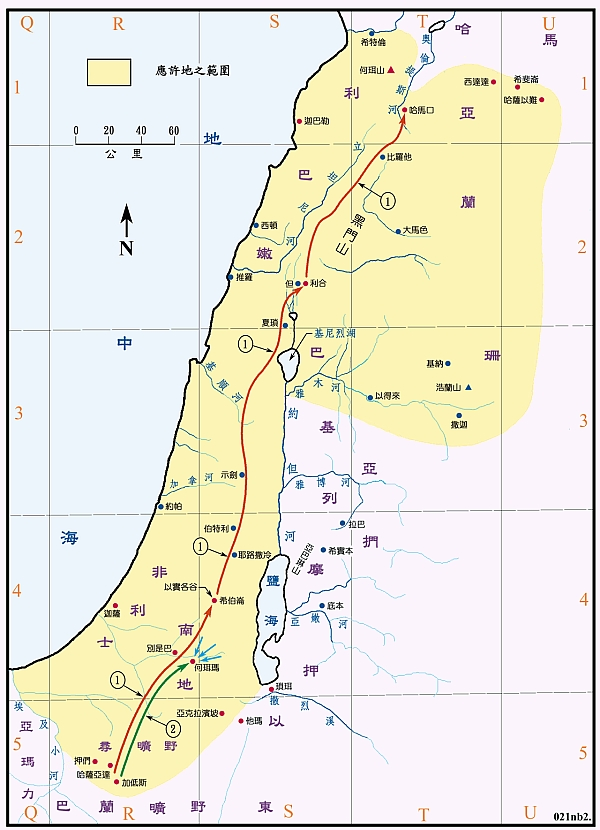
\includegraphics[width=3.8in]{AMoXiFigs/minshuji/tanzi}
\caption{1,十二探子巡视的路径;\\ 2,擅自攻打迦南人，但被迦南人擊敗}
\label{fig:1} 
\end{center}
\end{wrapfigure}
他們上去窺探那地，從尋的曠野到利合，直到哈馬口。他們從南地上去，到了希伯崙，在那裡有亞衲族人亞希幔、示篩、撻買。（原來希伯崙城被建造比埃及的鎖安城早七年。）他們到了以實各谷，從那裡砍了葡萄樹的一枝，上頭有一掛葡萄，兩個人用槓抬著，又帶了些石榴和無花果來。因為以色列人從那裡砍來的那掛葡萄，所以那地方叫做以實各谷。

\subsubsection{探子回來汇报 13:25-29}
過了四十天，他們窺探那地才回來。到了巴蘭曠野的加低斯，見摩西、亞倫並以色列的全會眾，回報摩西、亞倫並全會眾，又把那地的果子給他們看。又告訴摩西說：「我們到了你所打發我們去的那地，果然是流奶與蜜之地。這就是那地的果子。然而住那地的民強壯，城邑也堅固寬大，並且我們在那裡看見了亞衲族的人。亞瑪力人住在南地，赫人、耶布斯人、亞摩利人住在山地，迦南人住在海邊並約旦河旁。」

\subsubsection{迦勒安撫百姓 13:30-31}
迦勒在摩西面前安撫百姓，說：「我們立刻上去得那地吧，我們足能得勝！」但那些和他同去的人說：「我們不能上去攻擊那民，因為他們比我們強壯。」

\subsubsection{探子中有人報惡信 13:32-33}
探子中有人論到所窺探之地，向以色列人報惡信，說：「我們所窺探經過之地是吞吃居民之地，我們在那裡所看見的人民都身量高大。我們在那裡看見亞衲族人，就是偉人，他們是偉人的後裔。據我們看，自己就如蚱蜢一樣；據他們看，我們也是如此。」

\subsubsection{會眾大聲喧嚷百姓都哭號 14:1-4}
當下全會眾大聲喧嚷，那夜百姓都哭號。以色列眾人向摩西、亞倫發怨言，全會眾對他們說：「\textcolor{blue}{巴不得我們早死在埃及地，或是死在這曠野！耶和華為什麼把我們領到那地，使我們倒在刀下呢？我們的妻子和孩子必被擄掠。我們回埃及去豈不好嗎}？」眾人彼此說：「\textcolor{blue}{我們不如立一個首領回埃及去吧}！」

\subsubsection{約書亞和迦勒的信心 14:5-9}
\textcolor{blue}{摩西、亞倫}就俯伏在以色列全會眾面前。窺探地的人中，\textcolor{blue}{嫩的兒子約書亞}和\textcolor{blue}{耶孚尼的兒子迦勒}撕裂衣服，對以色列全會眾說：「我們所窺探經過之地是極美之地。耶和華若喜悅我們，就必將我們領進那地，把地賜給我們，那地原是流奶與蜜之地。但你們不可背叛耶和華，也不要怕那地的居民，因為他們是我們的食物，並且蔭庇他們的已經離開他們。有耶和華與我們同在，不要怕他們。」

\subsubsection{耶和華怒民違逆欲殲滅之 14:10-12}
但\textcolor{blue}{全會眾}說拿石頭打死他們二人。忽然，\textcolor{blue}{耶和華的榮光}在會幕中向以色列眾人顯現。\textcolor{blue}{耶和華對摩西說}：「這百姓藐視我要到幾時呢？我在他們中間行了這一切神蹟，他們還不信我要到幾時呢？我要用瘟疫擊殺他們，使他們不得承受那地，叫你的後裔成為大國，比他們強盛。」

\subsubsection{摩西為民求赦 14:13-19}
摩西對耶和華說：「\textcolor{blue}{埃及人必聽見}這事，因為你曾施展大能，將這百姓從他們中間領上來。埃及人要將這事傳給迦南地的居民。\textcolor{blue}{那民已經聽見}你耶和華是在這百姓中間，因為你面對面被人看見，有你的雲彩停在他們以上，你日間在雲柱中，夜間在火柱中，在他們前面行。如今你若把這百姓殺了，如殺一人，那些聽見你名聲的列邦必議論說：『耶和華因為不能把這百姓領進他向他們起誓應許之地，所以在曠野把他們殺了。』現在\textcolor{red}{求主}大顯能力，照你所說過的話說： 『耶和華不輕易發怒，並有豐盛的慈愛，赦免罪孽和過犯，萬不以有罪的為無罪，必追討他的罪，自父及子，直到三四代。』\textcolor{red}{求你}照你的大慈愛赦免這百姓的罪孽，好像你從埃及到如今常赦免他們一樣。」

\subsubsection{耶和華赦免百姓應許迦勒必得地為業 14:20-25}
耶和華說：「我照著你的話\textcolor{blue}{赦免了他們}。 然我指著我的永生起誓：遍地要被我的榮耀充滿！ 這些人雖看見我的榮耀和我在埃及與曠野所行的神蹟，仍然試探我這十次，不聽從我的話，\textcolor{blue}{他們斷不得看見}我向他們的祖宗所起誓應許之地。凡藐視我的，一個也不得看見。\\
\textcolor{red}{唯獨我的僕人迦勒}，因他另有一個心志，專一跟從我，我就把他領進他所去過的那地。\textcolor{red}{他的後裔}也必得那地為業。亞瑪力人和迦南人住在谷中，明天你們要轉回，從紅海的路往曠野去。」

\subsubsection{以色列眾發怨言者必死於野 14:26-35}
耶和華對摩西、亞倫說：「這惡會眾向我發怨言，我忍耐他們要到幾時呢？以色列人向我所發的怨言，我都聽見了。你們告訴他們：『耶和華說：我指著我的永生起誓：我必要照你們達到我耳中的話待你們。你們的屍首必倒在這曠野，並且你們中間凡被數點，從二十歲以外，向我發怨言的，必不得進我起誓應許叫你們住的那地。唯有耶孚尼的兒子迦勒和嫩的兒子約書亞才能進去。但你們的婦人孩子，就是你們所說要被擄掠的，我必把他們領進去，他們就得知你們所厭棄的那地。至於你們，你們的屍首必倒在這曠野。你們的兒女必在曠野漂流四十年，擔當你們淫行的罪，直到你們的屍首在曠野消滅。 按你們窺探那地的四十日，一年頂一日，你們要擔當罪孽四十年，就知道我與你們疏遠了。』我耶和華說過，我總要這樣待這一切聚集敵我的惡會眾。他們必在這曠野消滅，在這裡死亡。」

\subsubsection{十个報惡信探子遭瘟疫而死 14:36-38}
摩西所打發窺探那地的人回來，報那地的惡信，叫全會眾向摩西發怨言，這些報惡信的人都遭瘟疫，死在耶和華面前。其中唯有嫩的兒子約書亞和耶孚尼的兒子迦勒仍然存活。

\subsubsection{逆命的百姓欲上應許之地被殺退 14:39-45}
摩西將這些話告訴以色列眾人，他們就甚悲哀。清早起來，上山頂去，說：「我們在這裡，我們有罪了。情願上上耶和華所應許的地方去！」摩西說：「你們為何違背耶和華的命令呢？這事不能順利了！不要上去，因為耶和華不在你們中間，恐怕你們被仇敵殺敗了。亞瑪力人和迦南人都在你們面前，你們必倒在刀下。因你們退回不跟從耶和華，所以他必不與你們同在。」他們卻擅敢上山頂去，然而耶和華的約櫃和摩西沒有出營。於是亞瑪力人和住在那山上的迦南人都下來擊打他們，把他們殺退了，直到何珥瑪。

%\section{頒布律法 15 }
\subsection{頒布有關獻祭的條例 15}
\subsubsection{曉諭以色列人獻燔祭,平安祭 15:1-3}
耶和華對摩西說：「你曉諭以色列人說：你們到了我所賜給你們居住的地，若願意從牛群羊群中取牛羊做火祭獻給耶和華，無論是燔祭是平安祭，為要還特許的願，或是做甘心祭，或是逢你們節期獻的，都要奉給耶和華為馨香之祭。

\subsubsection{馨香火祭的條例 15:4-12}
\begin{wraptable}{r}{7cm}
\vspace*{-3mm}
\centering
\begin{tabular}{|c|c|c|c|}
\hline
\hline
\multirow{2}{3em}{祭物} &\multicolumn{2}{c|}{所配的素祭}&\multirow{2}{3em}{奠祭的酒(欣)} \\\cline{2-3}
  & 細麵(伊法)        &油(欣)              &\\ \hline
綿羊羔   &$\sfrac{1}{10}$ &$1\sfrac{1}{4}$&$1\sfrac{1}{4}$\\\hline
公綿羊   &$\sfrac{2}{10}$  &$1\sfrac{1}{3}$ &$1\sfrac{1}{3}$\\\hline
公牛      &$\sfrac{3}{10}$ &$\sfrac{1}{2}$    &$\sfrac{1}{2}$\\\hline
\end{tabular}
\caption{燔祭,平安祭,還特許的願\\所配的素祭和奠祭的酒}
\end{wraptable}
那獻供物的就要將細麵伊法十分之一，並油一欣四分之一，調和做素祭，獻給耶和華。無論是燔祭是平安祭，你要為每隻綿羊羔一同預備奠祭的酒一欣四分之一；為公綿羊預備細麵伊法十分之二，並油一欣三分之一，調和做素祭，又用酒一欣三分之一做奠祭，獻給耶和華為馨香之祭。你預備公牛做燔祭或是做平安祭，為要還特許的願，或是做平安祭，獻給耶和華，就要把細麵伊法十分之三，並油半欣，調和做素祭，和公牛一同獻上，又用酒半欣做奠祭，獻給耶和華為馨香的火祭。獻公牛、公綿羊、綿羊羔、山羊羔，每隻都要這樣辦理。照你們所預備的數目，按著隻數都要這樣辦理。

\subsubsection{同居的外人都歸一例 15:13-16}
凡本地人將馨香的火祭獻給耶和華，都要這樣辦理。若有外人和你們同居，或有人世世代代住在你們中間，願意將馨香的火祭獻給耶和華，你們怎樣辦理，他也要照樣辦理。至於會眾，你們和同居的外人都歸一例，作為你們世世代代永遠的定例。在耶和華面前，你們怎樣，寄居的也要怎樣。你們並與你們同居的外人當有一樣的條例，一樣的典章。

\subsubsection{舉祭的條例 15:17-21}
耶和華對摩西說：你曉諭以色列人說：你們到了我所領你們進去的那地，吃那地的糧食，就要把舉祭獻給耶和華。你們要用初熟的麥子磨麵，做餅當舉祭奉獻，你們舉上，好像舉禾場的舉祭一樣。你們世世代代要用初熟的麥子磨麵，當舉祭獻給耶和華。

\subsubsection{以色列全會眾誤犯罪獻祭的條例 15:22-26}
你們有錯誤的時候，不守耶和華所曉諭摩西的這一切命令，就是耶和華藉摩西一切所吩咐你們的，自那日以至你們的世世代代，若有誤行，是會眾所不知道的，後來全會眾就要
\vspace*{-2mm}
\begin{itemize} 
\itemsep-.35em
\item 將一隻公牛犢做燔祭，並照典章把素祭和奠祭一同獻給耶和華為馨香之祭，
\item 又獻一隻公山羊做贖罪祭。祭司要為以色列全會眾贖罪，
\end{itemize}
\vspace*{-2mm}
他們就必蒙赦免，因為這是錯誤。他們又因自己的錯誤，把供物，就是向耶和華獻的火祭和贖罪祭，一併奉到耶和華面前。以色列全會眾和寄居在他們中間的外人就必蒙赦免，因為這罪是百姓誤犯的。

\subsubsection{一個人誤犯罪獻祭的條例 15:27-29}
若有一個人誤犯了罪，他就要獻一歲的母山羊做贖罪祭。那誤行的人犯罪的時候，祭司要在耶和華面前為他贖罪，他就必蒙赦免。以色列中的本地人和寄居在他們中間的外人，若誤行了什麼事，必歸一樣的條例。

%\subsection{獻祭也不得赦免的罪 15:30-31 }
\subsubsection{違背耶和華的命令的總要剪除 15:30-31}
但那擅敢行事的，無論是本地人是寄居的，他褻瀆了耶和華，必從民中剪除。因他藐視耶和華的言語，違背耶和華的命令，那人總要剪除。他的罪孽要歸到他身上。

\subsubsection{違反安息日的條例 15:32-36 }
以色列人在曠野的時候，遇見一個人在安息日撿柴。遇見他撿柴的人，就把他帶到摩西、亞倫並全會眾那裡，將他收在監內，因為當怎樣辦他，還沒有指明。耶和華吩咐摩西說：「總要把那人治死，全會眾要在營外用石頭把他打死。」於是全會眾將他帶到營外，用石頭打死他，是照耶和華所吩咐摩西的。

\subsubsection{衣服繸子的條例 15:37-41 }
耶和華曉諭摩西說：「你吩咐以色列人，叫他們世世代代在衣服邊上做穗子，又在底邊的穗子上釘一根藍細帶子。你們佩戴這穗子，好叫你們看見就記念遵行耶和華一切的命令，不隨從自己的心意眼目行邪淫，像你們素常一樣，使你們記念遵行我一切的命令，成為聖潔，歸於你們的神。我是耶和華你們的神，曾把你們從埃及地領出來，要做你們的神。我是耶和華你們的神。」

%\section{安營時發生的事 16-17 }
\subsection{可拉黨叛亂 16-17}
\subsubsection{可拉並以色列會中250首領叛逆 16:1-3}
\begin{wraptable}{r}{9cm}
\vspace*{-20mm}
\centering
\begin{tabular}{|c|c|c|c|}
\hline
\hline
支派 & 父親名字&背叛人的名字&  結局 \\ \hline\hline
利未 &哥轄的兒子以斯哈 & 可拉 &被地開口吞沒\\ \hline
流便 & 以利押    &大坍&被地開口吞沒\\\hline
流便 & 以利押    &亞比蘭&被地開口吞沒\\\hline
流便 & 比勒    &安&被地開口吞沒\\\hline
以色列& -& 250個眾首領 &被火燒滅\\\hline
以色列& -& 14700百姓 &被瘟疫所殺\\\hline\hline
\end{tabular}
\caption{背叛的人}
\end{wraptable}
利未的曾孫、哥轄的孫子、以斯哈的兒子可拉，和魯本子孫中以利押的兒子大坍、亞比蘭，與比勒的兒子安，並以色列會中的二百五十個首領，就是有名望選入會中的人，在摩西面前一同起來，聚集攻擊摩西、亞倫，說：「你們擅自專權。全會眾個個既是聖潔，耶和華也在他們中間，你們為什麼自高，超過耶和華的會眾呢？」

\subsubsection{摩西两次劝慰可拉和他一黨的人 16:4-11}
摩西聽見這話就俯伏在地，對可拉和他一黨的人說：「到了早晨，耶和華必指示誰是屬他的，誰是聖潔的，就叫誰親近他。他所揀選的是誰，必叫誰親近他。可拉啊，你們要這樣行：你和你的一黨要拿香爐來，明日在耶和華面前，把火盛在爐中，把香放在其上。耶和華揀選誰，誰就為聖潔。你們這利未的子孫擅自專權了！」 
摩西又對可拉說：「利未的子孫哪，你們聽我說。以色列的神從以色列會中將你們分別出來，使你們親近他，辦耶和華帳幕的事，並站在會眾面前替他們當差。耶和華又使你，和你一切弟兄利未的子孫，一同親近他，這豈為小事，你們還要求祭司的職任嗎？你和你一黨的人聚集是要攻擊耶和華，亞倫算什麼，你們竟向他發怨言呢？」

\subsubsection{流便首領大坍、亞比蘭抗摩西命 16:12-14}
摩西打發人去召以利押的兒子大坍、亞比蘭。他們說：「我們不上去。你將我們從流奶與蜜之地領上來，要在曠野殺我們，這豈為小事，你還要自立為王轄管我們嗎？並且你沒有將我們領到流奶與蜜之地，也沒有把田地和葡萄園給我們為業。難道你要剜這些人的眼睛嗎？我們不上去。」

\subsubsection{亞倫和可拉黨250人各拿香爐全會眾在會幕門前 16:15-19}
摩西就甚發怒，對耶和華說：「求你不要享受他們的供物。我並沒有奪過他們一匹驢，也沒有害過他們一個人。」摩西對可拉說：「明天你和你一黨的人，並亞倫，都要站在耶和華面前。各人要拿一個香爐，共二百五十個，把香放在上面，到耶和華面前。你和亞倫也各拿自己的香爐。」於是他們各人拿一個香爐，盛上火，加上香，同摩西、亞倫站在會幕門前。可拉招聚全會眾到會幕門前，要攻擊摩西、亞倫。

\subsubsection{摩西、亞倫为全會眾代求 16:20-22}
耶和華的榮光就向全會眾顯現。耶和華曉諭摩西、亞倫說：「你們離開這會眾，我好在轉眼之間把他們滅絕。」摩西、亞倫就俯伏在地，說：「神，萬人之靈的神啊！一人犯罪，你就要向全會眾發怒嗎？」 

\subsubsection{摩西照神吩咐警戒會眾離開可拉、大坍、亞比蘭帳篷 16:23-27}
耶和華曉諭摩西說：「你吩咐會眾說：你們離開可拉、大坍、亞比蘭帳篷的四圍。」摩西起來，往大坍、亞比蘭那裡去，以色列的長老也隨著他去。他吩咐會眾說：「你們離開這惡人的帳篷吧，他們的物件，什麼都不可摸，恐怕你們陷在他們的罪中，與他們一同消滅。」於是眾人離開可拉、大坍、亞比蘭帳篷的四圍。大坍、亞比蘭帶著妻子、兒女、小孩子，都出來，站在自己的帳篷門口。

\subsubsection{摩西宣布他們活活地墜落陰間 16:28-30}
摩西說：「我行的這一切事本不是憑我自己心意行的，乃是耶和華打發我行的，必有證據使你們知道。這些人死若與世人無異，或是他們所遭的與世人相同，就不是耶和華打發我來的。倘若耶和華創作一件新事，使地開口，把他們和一切屬他們的都吞下去，叫他們活活地墜落陰間，你們就明白這些人是藐視耶和華了。」

\subsubsection{地開口把他們並一切屬可拉的人丁、財物，都吞下去 16:31-34}
摩西剛說完了這一切話，他們腳下的地就開了口，把他們和他們的家眷，並一切屬可拉的人丁、財物，都吞下去。這樣，他們和一切屬他們的都活活地墜落陰間。地口在他們上頭照舊合閉，他們就從會中滅亡。在他們四圍的以色列眾人聽他們呼號，就都逃跑，說：「恐怕地也把我們吞下去！」

\subsubsection{火燒獻香的250人，以利亞撒用香爐的銅包壇 16:35-40}
又有火從耶和華那裡出來，燒滅了那獻香的二百五十個人。耶和華曉諭摩西說：「你吩咐祭司亞倫的兒子以利亞撒從火中撿起那些香爐來，把火撒在別處，因為那些香爐是聖的。把那些犯罪自害己命之人的香爐，叫人錘成片子，用以包壇。那些香爐本是他們在耶和華面前獻過的，所以是聖的，並且可以給以色列人做記號。」於是祭司以利亞撒將被燒之人所獻的銅香爐拿來，人就錘出來，用以包壇，給以色列人做紀念，使亞倫後裔之外的人不得近前來在耶和華面前燒香，免得他遭可拉和他一黨所遭的。這乃是照耶和華藉著摩西所吩咐的。

\subsubsection{以色列全會眾發怨言，摩西、亞倫代求 16:41-45}
第二天，以色列全會眾都向摩西、亞倫發怨言說：「你們殺了耶和華的百姓了！」會眾聚集攻擊摩西、亞倫的時候，向會幕觀看，不料，有雲彩遮蓋了，耶和華的榮光顯現。摩西、亞倫就來到會幕前。耶和華吩咐摩西說：「你們離開這會眾，我好在轉眼之間把他們滅絕。」他們二人就俯伏於地。 

\subsubsection{因發怨言民遭疫癘 16:46-50}
摩西對亞倫說：「拿你的香爐，把壇上的火盛在其中，又加上香，快快帶到會眾那裡，為他們贖罪。因為有憤怒從耶和華那裡出來，瘟疫已經發作了。」亞倫照著摩西所說的拿來，跑到會中，不料，瘟疫在百姓中已經發作了。他就加上香，為百姓贖罪。他站在活人死人中間，瘟疫就止住了。除了因可拉事情死的以外，遭瘟疫死的，共有一萬四千七百人。亞倫回到會幕門口，到摩西那裡，瘟疫已經止住了。

\subsubsection{十二首領按支派各取仗存在法櫃的帳幕內 17:1-7}
耶和華對摩西說：「你曉諭以色列人，從他們手下取杖，每支派一根。從他們所有的首領，按著支派，共取十二根。你要將各人的名字寫在各人的杖上，並要將亞倫的名字寫在利未的杖上，因為各族長必有一根杖。你要把這些杖存在會幕內法櫃前，就是我與你們相會之處。後來我所揀選的那人，他的杖必發芽。這樣，我必使以色列人向你們所發的怨言止息，不再達到我耳中。」於是摩西曉諭以色列人，他們的首領就把杖交給他，按著支派，每首領一根，共有十二根，亞倫的杖也在其中。摩西就把杖存在法櫃的帳幕內，在耶和華面前。

\subsubsection{亞倫之杖發芽開花結熟杏 17:8-11}
第二天，摩西進法櫃的帳幕去。誰知利未族亞倫的杖已經發了芽，生了花苞，開了花，結了熟杏。摩西就把所有的杖從耶和華面前拿出來，給以色列眾人看。他們看見了，各首領就把自己的杖拿去。耶和華吩咐摩西說：「把亞倫的杖還放在法櫃前，給這些背叛之子留做記號。這樣，你就使他們向我發的怨言止息，免得他們死亡。」摩西就這樣行。耶和華怎樣吩咐他，他就怎樣行了。

\subsubsection{以色列說“凡挨近耶和華帳幕的是必死的” 17:12-13}
以色列人對摩西說：「我們死啦！我們滅亡啦！都滅亡啦！凡挨近耶和華帳幕的是必死的。我們都要死亡嗎？」

\subsection{頒布祭司與利未人的律法 18-19 }
\subsubsection{祭司與利未人的職任 18:1-7 }
\noindent
耶和華對亞倫說：「你和你的兒子並你本族的人，要一同擔當干犯聖所的罪孽，你和你的兒子也要一同擔當干犯祭司職任的罪孽。你要帶你弟兄利未人，就是你祖宗支派的人前來，使他們與你聯合，服侍你，只是你和你的兒子，要一同在法櫃的帳幕前供職。他們要守所吩咐你的，並守全帳幕，只是不可挨近聖所的器具和壇，免得他們和你們都死亡。他們要與你聯合，也要看守會幕，辦理帳幕一切的事，只是外人不可挨近你們。你們要看守聖所和壇，免得憤怒再臨到以色列人。我已將你們的弟兄利未人，從以色列人中揀選出來歸耶和華，是給你們為賞賜的，為要辦理會幕的事。你和你的兒子要為一切屬壇和幔子內的事一同守祭司的職任。你們要這樣供職。我將祭司的職任給你們當做賞賜侍奉我。凡挨近的外人必被治死。」

\subsubsection{祭司當得之物  18:8-14 }
耶和華曉諭亞倫說：我已將歸我的舉祭，就是以色列人一切分別為聖的物，交給你經管。因你受過膏，把這些都賜給你和你的子孫，當做永得的份。
\begin{itemize} 
\itemsep-.25em  
\item 以色列人歸給我至聖的供物，就是一切的素祭、贖罪祭、贖愆祭，其中所有存留不經火的，都為至聖之物，要歸給你和你的子孫。你要拿這些當至聖物吃，\textcolor{blue}{凡男丁都可以吃}。你當以此物為聖。
\item 以色列人所獻的舉祭並搖祭都是你的，我已賜給你和你的兒女，當做永得的份。凡在你\textcolor{blue}{家中的潔淨人都可以吃}。凡油中、新酒中、五穀中至好的，就是以色列人所獻給耶和華初熟之物，我都賜給你。凡從他們地上所帶來給耶和華初熟之物，也都要歸於你。你家中的潔淨人都可以吃。以色列中一切永獻的都必歸於你。 
\end{itemize}

\subsubsection{頭生之物 18:15-20}
\begin{itemize} 
\itemsep-.25em  
\item 他們所有奉給耶和華的，連人帶牲畜，凡頭生的，都要歸給你。只是人頭生的，總要贖出來，不潔淨牲畜頭生的也要贖出來。其中在一月之外所當贖的，要照你所估定的價，按聖所的平，用銀子五舍客勒贖出來（一舍客勒是二十季拉）。 
\item 只是頭生的牛，或是頭生的綿羊和山羊，必不可贖，都是聖的，要把牠的血灑在壇上，把牠的脂油焚燒，當做馨香的火祭獻給耶和華。牠的肉必歸你，像被搖的胸、被舉的右腿歸你一樣。凡以色列人所獻給耶和華聖物中的舉祭，我都賜給你和你的兒女，當做永得的份。這是給你和你的後裔，在耶和華面前作為永遠的鹽(不廢壞)約。」
\item 耶和華對亞倫說：你在以色列人的境內不可有產業，在他們中間也不可有份。我就是你的份，是你的產業。
\end{itemize}

\subsubsection{利未人的份 18:21-24}
\begin{itemize} 
\itemsep-.25em  
\item 凡以色列中出產的十分之一，我已賜給利未的子孫為業。因他們所辦的是會幕的事，所以賜給他們為酬他們的勞。
\item 從今以後，以色列人不可挨近會幕，免得他們擔罪而死。唯獨利未人要辦會幕的事，擔當罪孽，這要做你們世世代代永遠的定例。
\item 他們在以色列人中不可有產業。因為以色列人中出產的十分之一，就是獻給耶和華為舉祭的，我已賜給利未人為業，所以我對他們說：在以色列人中不可有產業。」
\end{itemize}

\subsubsection{利未人的奉獻 18:25-32}
耶和華吩咐摩西說：「你曉諭利未人說：你們從以色列人中所取的十分之一，就是我給你們為業的，要再從那十分之一中取十分之一作為舉祭獻給耶和華。這舉祭要算為你們場上的穀，又如滿酒榨的酒。這樣，你們從以色列人中所得的十分之一也要做舉祭獻給耶和華，從這十分之一中，將所獻給耶和華的舉祭歸給祭司亞倫。奉給你們的一切禮物，要從其中將至好的，就是分別為聖的，獻給耶和華為舉祭。所以你要對利未人說：『你們從其中將至好的舉起，這就算為你們場上的糧，又如酒榨的酒。你們和你們家屬隨處可以吃，這原是你們的賞賜，是酬你們在會幕裡辦事的勞。你們從其中將至好的舉起，就不致因這物擔罪。你們不可褻瀆以色列人的聖物，免得死亡。』」

\subsubsection{用紅母牛灰調做除汙穢水 19:1-10}
\noindent
耶和華曉諭摩西、亞倫說： 「耶和華命定律法中的一條律例乃是這樣說：你要吩咐以色列人，把一隻沒有殘疾、未曾負軛、純紅的母牛牽到你這裡來，交給祭司以利亞撒。他必牽到營外，人就把牛宰在他面前。 祭司以利亞撒要用指頭蘸這牛的血，向會幕前面彈七次。人要在他眼前把這母牛焚燒，牛的皮、肉、血、糞都要焚燒。祭司要把香柏木、牛膝草、朱紅色線都丟在燒牛的火中。祭司必不潔淨到晚上，要洗衣服，用水洗身，然後可以進營。 燒牛的人必不潔淨到晚上，也要洗衣服，用水洗身。必有一個潔淨的人收起母牛的灰，存在營外潔淨的地方，為以色列會眾調做除汙穢的水，這本是除罪的。收起母牛灰的人必不潔淨到晚上，要洗衣服。這要給以色列人和寄居在他們中間的外人作為永遠的定例。 

\subsubsection{適用除汙水的人 19:11-16}
\begin{itemize} 
\itemsep-.25em  
\item 摸了人死屍的，就必七天不潔淨。那人到第三天要用這除汙穢的水潔淨自己，第七天就潔淨了。他若在第三天不潔淨自己，第七天就不潔淨了。凡摸了人死屍，不潔淨自己的，就玷汙了耶和華的帳幕，這人必從以色列中剪除。因為那除汙穢的水沒有灑在他身上，他就為不潔淨，汙穢還在他身上。
\item 人死在帳篷裡的條例乃是這樣：凡進那帳篷的和一切在帳篷裡的，都必七天不潔淨。凡敞口的器皿，就是沒有紮上蓋的，也是不潔淨。
\item 無論何人在田野裡摸了被刀殺的，或是屍首，或是人的骨頭，或是墳墓，就要七天不潔淨。
\end{itemize}

\subsubsection{除汙水的使用 19:17-22}
要為這不潔淨的人拿些燒成的除罪灰放在器皿裡倒上活水。必當有一個潔淨的人拿牛膝草蘸在這水中，把水灑在帳篷上和一切器皿並帳篷內的眾人身上，又灑在摸了骨頭，或摸了被殺的，或摸了自死的，或摸了墳墓的那人身上。
\vspace*{-2mm}
\begin{itemize} 
\itemsep-.25em  
\item 第三天和第七天，潔淨的人要灑水在不潔淨的人身上，第七天就使他成為潔淨。那人要洗衣服，用水洗澡，到晚上就潔淨了。
\item 但那汙穢而不潔淨自己的，要將他從會中剪除，因為他玷汙了耶和華的聖所。除汙穢的水沒有灑在他身上，他是不潔淨的。這要給你們作為永遠的定例。
\item 並且那灑除汙穢水的人要洗衣服，凡摸除汙穢水的，必不潔淨到晚上。不潔淨人所摸的一切物就不潔淨，摸了這物的人必不潔淨到晚上。
\end{itemize}

%\section{行程中發生的事 20-27 }
\subsection{旷野漂流中發生的事 20-22}
\subsubsection{正月米利暗死在尋的曠野加低斯 20:1}
\begin{wrapfigure}{r}{0.5\textwidth}
\vspace*{-30mm}
\center 
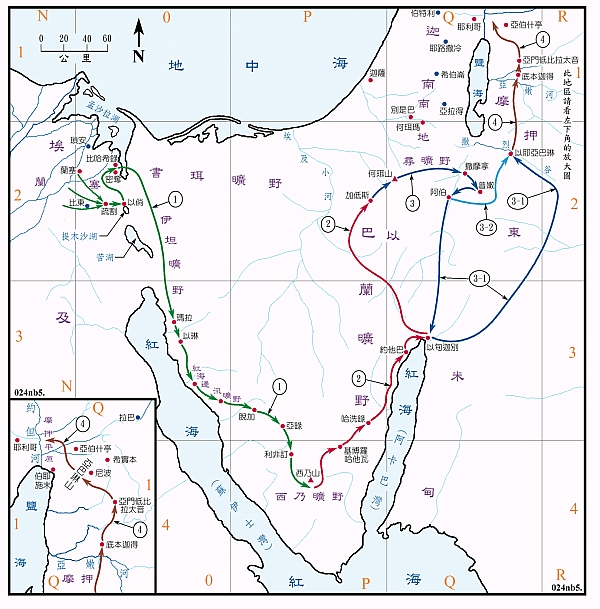
\includegraphics[width=3.5in]{AMoXiFigs/fig4}
\caption{行程中發生的事}
\label{fig:1} 
%\end{center}
\end{wrapfigure}
正月間，以色列全會眾到了尋的曠野，就住在加低斯。米利暗死在那裡，就葬在那裡。


\subsubsection{米利巴摩西因无水受牵累 20:2-13}
\subsubsubsection{米利巴會眾无水攻擊摩西 20:2-5}
會眾沒有水喝，就聚集攻擊摩西、亞倫。百姓向摩西爭鬧說：「我們的弟兄曾死在耶和華面前，我們恨不得與他們同死。你們為何把耶和華的會眾領到這曠野，使我們和牲畜都死在這裡呢？你們為何逼著我們出埃及，領我們到這壞地方呢？這地方不好撒種，也沒有無花果樹、葡萄樹、石榴樹，又沒有水喝。」

\subsubsubsection{曉諭摩西吩咐磐石出水 20:6-9}
摩西、亞倫離開會眾，到會幕門口，俯伏在地。耶和華的榮光向他們顯現。耶和華曉諭摩西說：「你拿著杖去，和你的哥哥亞倫招聚會眾，在他們眼前吩咐磐石發出水來，水就從磐石流出，給會眾和他們的牲畜喝。」

\subsubsubsection{摩西擊打磐石受亏损 20:10-13 }
\begin{table}[H]
%\arrayrulecolor[HTML]{DB5800}
\begin{threeparttable}
\begin{tabular}{@{}p{0.53\textwidth}*{4}{L{\dimexpr0.6\linewidth-10\tabcolsep\relax}}@{}}
\toprule
摩西 &  以東王 \\\hline
於是摩西照耶和華所吩咐的，從耶和華面前取了杖去。摩西、亞倫就招聚會眾到磐石前。摩西說：「你們這些背叛的人聽我說：我為你們使水從這磐石中流出來嗎？」摩西舉手，用杖擊打磐石兩下，就有許多水流出來，會眾和他們的牲畜都喝了。
&耶和華對摩西、亞倫說：「因為你們不信我，不在以色列人眼前尊我為聖，所以你們必不得領這會眾進我所賜給他們的地去。」這水名叫米利巴(爭鬧)水，是因以色列人向耶和華爭鬧，耶和華就在他們面前顯為聖。\tabularnewline
\bottomrule
\end{tabular}
\caption{摩西擊打磐石受亏损}
\end{threeparttable}
\end{table} 

\subsubsection{以東王不允以色列人過其境 20:14-21}
\begin{table}[H]
%\arrayrulecolor[HTML]{DB5800}
\begin{threeparttable}
\begin{tabular}{@{}p{0.53\textwidth}*{4}{L{\dimexpr0.58\linewidth-10\tabcolsep\relax}}@{}}
\toprule
摩西 &  以東王 \\\hline
摩西從加低斯差遣使者去見以東王，說：「你的弟兄以色列人這樣說：我們所遭遇的一切艱難，就是我們的列祖下到埃及，我們在埃及久住，埃及人惡待我們的列祖和我們，我們哀求耶和華的時候，他聽了我們的聲音，差遣使者把我們從埃及領出來，這事你都知道。如今，我們在你邊界上的城加低斯。求你容我們從你的地經過。我們不走田間和葡萄園，也不喝井裡的水，只走大道(王道)，不偏左右，直到過了你的境界。」
&以東王說：「你不可從我的地經過，免得我帶刀出去攻擊你。」\tabularnewline\hline
以色列人說：「我們要走大道上去。我們和牲畜若喝你的水，必給你價值。不求別的，只求你容我們步行過去。」
&以東王說：「你們不可經過。」就率領許多人出來，要用強硬的手攻擊以色列人。這樣，以東王不肯容以色列人從他的境界過去。於是他們轉去，離開他。\tabularnewline
\bottomrule
\end{tabular}
\caption{以東王不允以色列人過其境}
\end{threeparttable}
\end{table} 

\subsubsection{亞倫死在何珥山 20:22-29 }
以色列全會眾從加低斯起行，到了何珥山。耶和華在附近以東邊界的何珥山上曉諭摩西、亞倫說：「亞倫要歸到他列祖(本民)那裡。他必不得入我所賜給以色列人的地，因為在米利巴水，你們違背了我的命。你帶亞倫和他的兒子以利亞撒上何珥山，把亞倫的聖衣脫下來，給他的兒子以利亞撒穿上。亞倫必死在那裡，歸他列祖。」摩西就照耶和華所吩咐的行。三人當著會眾的眼前上了何珥山。摩西把亞倫的聖衣脫下來，給他的兒子以利亞撒穿上，亞倫就死在山頂那裡。於是摩西和以利亞撒下了山。全會眾，就是以色列全家，見亞倫已經死了，便都為亞倫哀哭了三十天。
 
\subsubsection{何珥瑪的迦南人亞拉得王被毀 21:1-3 }
\noindent
南地的迦南人亞拉得王、聽說以色列人從亞他林路來、就和以色列人爭戰、擄了他們幾個人。耶和華應允了以色列人、他們就把迦南人、和迦南人的城邑、盡行毀滅。那地方的名便叫何珥瑪〔毀滅〕。 

\subsubsection{製造銅火蛇  21:5-9 }
他們從何珥山起行，往紅海那條路走，要繞過以東地。百姓因這路難行，心中甚是煩躁，就怨讟神和摩西說：「你們為什麼把我們從埃及領出來，使我們死在曠野呢？這裡沒有糧，沒有水，我們的心厭惡這淡薄的食物！」於是耶和華使火蛇進入百姓中間，蛇就咬他們，以色列人中死了許多。百姓到摩西那裡，說：「我們怨讟耶和華和你，有罪了。求你禱告耶和華，叫這些蛇離開我們。」於是摩西為百姓禱告。耶和華對摩西說：「你製造一條火蛇，掛在杆子上。凡被咬的，一望這蛇，就必得活。」摩西便製造一條銅蛇，掛在杆子上。凡被蛇咬的，一望這銅蛇就活了。

\subsubsection{曠野路線 21:10-20 }
以色列人起行，安營在阿伯。又從阿伯起行，安營在以耶亞巴琳，與摩押相對的曠野，向日出之地。從那裡起行，安營在撒烈谷。從那裡起行，安營在亞嫩河那邊。這亞嫩河是在曠野，從亞摩利的境界流出來的。原來亞嫩河是摩押的邊界，在摩押和亞摩利人搭界的地方。所以《耶和華的戰記》上說：「蘇法的哇哈伯與亞嫩河的谷，並向亞珥城眾谷的下坡，是靠近摩押的境界。」以色列人從那裡起行，到了比珥(井)。從前耶和華吩咐摩西說：「招聚百姓，我好給他們水喝」，說的就是這井。當時，以色列人唱歌說：「井啊，湧上水來！你們要向這井歌唱。這井是首領和民中的尊貴人用圭用杖所挖所掘的。」以色列人從曠野往瑪他拿去，從瑪他拿到拿哈列，從拿哈列到巴末，從巴末到摩押地的谷，又到那下望曠野之毗斯迦的山頂。

\subsubsection{希實本的亞摩利人王西宏 21:21-32}
以色列人差遣使者去見亞摩利人的王西宏，說：「求你容我們從你的地經過。我們不偏入田間和葡萄園，也不喝井裡的水，只走大道 (王道)，直到過了你的境界。」西宏不容以色列人從他的境界經過，就招聚他的眾民出到曠野，要攻擊以色列人，到了雅雜與以色列人爭戰。以色列人用刀殺了他，得了他的地，從亞嫩河到雅博河，直到亞捫人的境界，因為亞捫人的境界多有堅壘。以色列人奪取這一切的城邑，也住亞摩利人的城邑，就是希實本與希實本的一切鄉村。這希實本是亞摩利王西宏的京城，西宏曾與摩押的先王爭戰，從他手中奪取了全地，直到亞嫩河。所以那些作詩歌的說：「你們來到希實本，願西宏的城被修造，被建立！因為有火從希實本發出，有火焰出於西宏的城，燒盡摩押的亞珥和亞嫩河丘壇的祭司(主)。摩押啊，你有禍了！基抹的民哪，你們滅亡了！基抹的男子逃奔，女子被擄，交付亞摩利的王西宏。我們射了他們，希實本直到底本盡皆毀滅。我們使地變成荒場，直到挪法。這挪法直延到米底巴。」這樣，以色列人就住在亞摩利人之地。摩西打發人去窺探雅謝，以色列人就占了雅謝的鎮市，趕出那裡的亞摩利人。

\subsubsection{巴珊王噩 21:33-35}
以色列人轉回，向巴珊去。巴珊王噩和他的眾民都出來，在以得來與他們交戰。耶和華對摩西說：「不要怕他。因我已將他和他的眾民，並他的地，都交在你手中。你要待他像從前待住希實本的亞摩利王西宏一般。」於是他們殺了他和他的眾子，並他的眾民，沒有留下一個，就得了他的地。

\section{摩押平原的事件 22-36}
\subsection{摩押王西撥的兒子召巴勒比珥的兒子巴蘭22-25}

\subsubsection{摩押王西撥的兒子求米甸長老召巴蘭 22:1-6}
以色列人起行，在摩押平原，約旦河東，對著耶利哥安營。以色列人向亞摩利人所行的一切事，西撥的兒子巴勒都看見了。摩押人因以色列民甚多，就大大懼怕，心內憂急，對米甸的長老說：「現在這眾人要把我們四圍所有的一概舔盡，就如牛舔盡田間的草一般。」那時西撥的兒子巴勒做摩押王。他差遣使者往大河邊的毗奪去，到比珥的兒子巴蘭本鄉那裡，召巴蘭來，說：「有一宗民從埃及出來，遮滿地面，與我對居。這民比我強盛，現在求你來為我咒詛他們，或者我能得勝，攻打他們，趕出此地。因為我知道，你為誰祝福，誰就得福；你咒詛誰，誰就受咒詛。」

\subsubsection{一次差摩押米甸長老召巴蘭被拒 22:7-14}
\begin{itemize} 
\itemsep-.35em
\item 摩押的長老和米甸的長老手裡拿著卦金，到了巴蘭那裡，將巴勒的話都告訴了他。巴蘭說：「你們今夜在這裡住宿，我必照耶和華所曉諭我的回報你們。」摩押的使臣就在巴蘭那裡住下了。
\item 神臨到巴蘭那裡，說：「在你這裡的人都是誰？」巴蘭回答說：「是摩押王西撥的兒子巴勒打發人到我這裡來，說： 『從埃及出來的民遮滿地面，你來為我咒詛他們，或者我能與他們爭戰，把他們趕出去。』」神對巴蘭說：「你不可同他們去，也不可咒詛那民，因為那民是蒙福的。」
\item 巴蘭早晨起來，對巴勒的使臣說：「你們回本地去吧，因為耶和華不容我和你們同去。」摩押的使臣就起來，回巴勒那裡去，說：「巴蘭不肯和我們同來。」
\end{itemize}

\subsubsection{二次差更多且尊貴的人召巴蘭 22:15-20}
\begin{itemize} 
\itemsep-.35em
\item 巴勒又差遣使臣，比先前的又多又尊貴。他們到了巴蘭那裡，對他說：「西撥的兒子巴勒這樣說：求你不容什麼事攔阻你不到我這裡來！因為我必使你得極大的尊榮，你向我要什麼，我就給你什麼，只求你來為我咒詛這民。」
\item 巴蘭回答巴勒的臣僕說：「巴勒就是將他滿屋的金銀給我，我行大事小事也不得越過耶和華我神的命。現在我請你們今夜在這裡住宿，等我得知耶和華還要對我說什麼。」
\item 當夜，神臨到巴蘭那裡，說：「這些人若來召你，你就起來同他們去，你只要遵行我對你所說的話。」
\end{itemize}

\subsubsection{天使阻巴蘭 22:21-27}
\begin{table}[H]
\begin{tabular}{@{}p{0.385\textwidth}*{4}{L{\dimexpr0.735\linewidth-10\tabcolsep\relax}}@{}}
\toprule
巴蘭 &驢 \\\hline
巴蘭早晨起來，備上驢，和摩押的使臣一同去了。神因他去就發了怒，耶和華的使者站在路上抵擋他。他騎著驢有兩個僕人跟隨他。&驢看見耶和華的使者站在路上，手裡有拔出來的刀，就從路上跨進田間。\\\hline
巴蘭便打驢，要叫牠回轉上路。&耶和華的使者就站在葡萄園的窄路上，這邊有牆，那邊也有牆。 驢看見耶和華的使者，就貼靠牆，將巴蘭的腳擠傷了。\\\hline
巴蘭又打驢。&耶和華的使者又往前去，站在狹窄之處，左右都沒有轉折的地方。驢看見耶和華的使者，就臥在巴蘭底下，\tabularnewline\hline
巴蘭發怒，用杖打驢。&耶和華叫驢開口對巴蘭說：「我向你行了什麼，你竟打我這三次呢？」\tabularnewline\hline
巴蘭對驢說：「因為你戲弄我。我恨不能手中有刀，把你殺了。」&驢對巴蘭說：「我不是你從小時直到今日所騎的驢嗎？我素常向你這樣行過嗎？」\tabularnewline\hline
巴蘭說：「沒有。」&\tabularnewline\hline
\bottomrule
\end{tabular}
\caption{天使阻巴蘭,驢开口說話}
\end{table} 

\subsubsection{耶和華的使者對巴蘭說話 22:31-35}
\begin{table}[H]
%\begin{threeparttable}
\begin{tabular}{@{}p{0.63\textwidth}*{4}{L{\dimexpr0.48\linewidth-10\tabcolsep\relax}}@{}}
\toprule
耶和華的使者 &  巴蘭 \\\hline
當時，耶和華使巴蘭的眼目明亮，&他就看見耶和華的使者站在路上，手裡有拔出來的刀。巴蘭便低頭俯伏在地。\\\hline
耶和華的使者對他說：「你為何這三次打你的驢呢？我出來抵擋你，因你所行的，在我面前偏僻。驢看見我就三次從我面前偏過去，驢若沒有偏過去，我早把你殺了，留牠存活。」&巴蘭對耶和華的使者說：「我有罪了，我不知道你站在路上阻擋我。你若不喜歡我去，我就轉回。」\\\hline
耶和華的使者對巴蘭說：「你同這些人去吧，你只要說我對你說的話。」&於是巴蘭同著巴勒的使臣去了。\tabularnewline
\bottomrule
\end{tabular}
\caption{耶和華的使者對巴蘭說話}
%\end{threeparttable}
\end{table} 


\subsubsection{巴勒迎巴蘭 22:36-40}
\begin{figure}[H]%{.5\linewidth}
\centering
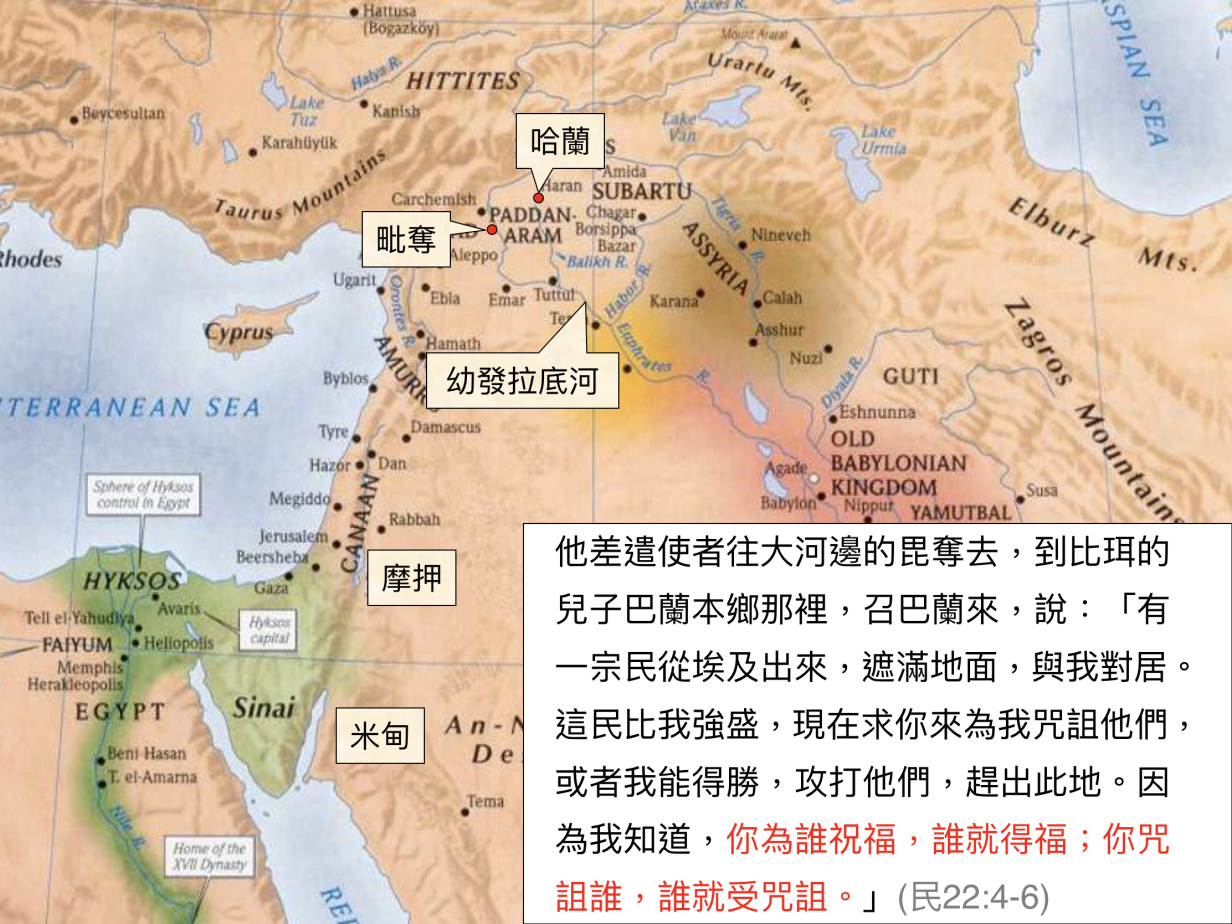
\includegraphics[width=5in]{AMoXiFigs/minshuji/balan}
\caption{以色列在曠野的經歷}
\label{fig:sub1}
\end{figure}
\begin{table}[H]
%\begin{threeparttable}
\begin{tabular}{@{}p{0.5\textwidth}*{4}{L{\dimexpr0.58\linewidth-10\tabcolsep\relax}}@{}}
\toprule
巴勒&巴蘭 \\\hline
巴勒聽見巴蘭來了，就往摩押京城去迎接他。這城是在邊界上，在亞嫩河旁。巴勒對巴蘭說：「我不是急急地打發人到你那裡去召你嗎？你為何不到我這裡來呢？我豈不能使你得尊榮嗎？」&巴蘭說：「我已經到你這裡來了。現在我豈能擅自說什麼呢？神將什麼話傳給我，我就說什麼。」巴蘭和巴勒同行，來到基列胡瑣。巴勒宰（獻）了牛羊，送給巴蘭和陪伴的使臣。\\\hline
\bottomrule
\end{tabular}
\caption{巴勒迎巴蘭}
%\end{threeparttable}
\end{table} 


\subsubsection{巴蘭第一次預言 22:41-23:12}
\begin{table}[H]
\begin{tabular}{@{}p{0.3\textwidth}*{4}{L{\dimexpr0.8\linewidth-10\tabcolsep\relax}}@{}}
\toprule
巴勒&巴蘭 \\\hline
到了早晨，巴勒領巴蘭到巴力的高處，&巴蘭從那裡觀看以色列營的邊界。巴蘭對巴勒說：「你在這裡給我築七座壇，為我預備七隻公牛、七隻公羊。」\\\hline
巴勒照巴蘭的話行了。巴勒和巴蘭在每座壇上獻一隻公牛、一隻公羊。&巴蘭對巴勒說：「你站在你的燔祭旁邊，我且往前去，或者耶和華來迎見我。他指示我什麼，我必告訴你。」於是巴蘭上一淨光的高處。\\\hline
&神迎見巴蘭。巴蘭說：「我預備了七座壇，在每座壇上獻了一隻公牛、一隻公羊。」耶和華將話傳給巴蘭，又說:「你回到巴勒那裡，要如此如此說。」 \\\hline
&他就回到巴勒那裡，見他同摩押的使臣都站在燔祭旁邊。巴蘭便題起詩歌說："巴勒引我出亞蘭，摩押王引我出東山說:『來啊，為我咒詛雅各！來啊，怒罵以色列！』神沒有咒詛的我焉能咒詛？耶和華沒有怒罵的我焉能怒罵？我從高峰看他，從小山望他，這是獨居的民，不列在萬民中。誰能數點雅各的塵土?誰能計算以色列的四分之一?我願如義人之死而死，我願如義人之終而終。"\\\hline
巴勒對巴蘭說：「你向我做的是什麼事呢？我領你來咒詛我的仇敵，不料，你竟為他們祝福！」&他回答說：「耶和華傳給我的話，我能不謹慎傳說嗎？」\\\hline
\bottomrule
\end{tabular}
\caption{巴蘭第一次預言}
\end{table} 



\subsubsection{巴蘭第二次預言 23:13-26}
\begin{table}[H]
%\begin{threeparttable}
\begin{tabular}{@{}p{0.5\textwidth}*{4}{L{\dimexpr0.63\linewidth-10\tabcolsep\relax}}@{}}
\toprule
巴勒&巴蘭 \\\hline
巴勒說：「求你同我往別處去，在那裡可以看見他們。你不能全看見，只能看見他們邊界上的人。在那裡要為我咒詛他們。」於是領巴蘭到了瑣腓田，上了毗斯迦山頂，築了七座壇，每座壇上獻一隻公牛、一隻公羊。&巴蘭對巴勒說：「你站在這燔祭旁邊，等我往那邊去迎見耶和華。」耶和華臨到巴蘭那裡，將話傳給他，又說：「你回到巴勒那裡，要如此如此說。」他就回到巴勒那裡，見他站在燔祭旁邊，摩押的使臣也和他在一處。\\\hline
巴勒問他說：「耶和華說了什麼話呢？」&巴蘭就題詩歌說：「巴勒，你起來聽；西撥的兒子，你聽我言。神非人，必不至說謊；也非人子，必不至後悔。他說話豈不照著行呢？他發言豈不要成就呢？我奉命祝福，神也曾賜福，此事我不能翻轉。他未見雅各中有罪孽，也未見以色列中有奸惡。耶和華他的神和他同在，有歡呼王的聲音在他們中間。神領他們出埃及，他們似乎有野牛之力。斷沒有法術可以害雅各，也沒有占卜可以害以色列。現在必有人論及雅各，就是論及以色列說：『神為他行了何等的大事！』這民起來彷彿母獅，挺身好像公獅，未曾吃野食，未曾喝被傷者之血，決不躺臥。」\\\hline
巴勒對巴蘭說：「你一點不要咒詛他們，也不要為他們祝福。」&巴蘭回答巴勒說：「我豈不是告訴你說，凡耶和華所說的，我必須遵行嗎？」\\\hline
\bottomrule
\end{tabular}
\caption{巴蘭第二次預言}
%\end{threeparttable}
\end{table} 


\subsubsection{巴蘭第三次預言 23:27-24:13}
\begin{table}[H]
%\begin{threeparttable}
\begin{tabular}{@{}p{0.5\textwidth}*{4}{L{\dimexpr0.63\linewidth-10\tabcolsep\relax}}@{}}
\toprule
巴勒&巴蘭 \\\hline
巴勒對巴蘭說：「來吧，我領你往別處去，或者神喜歡你在那裡為我咒詛他們。」巴勒就領巴蘭到那下望曠野的毗珥山頂上。&巴蘭對巴勒說：「你在這裡為我築七座壇，又在這裡為我預備七隻公牛、七隻公羊。」\\\hline
巴勒就照巴蘭的話行，在每座壇上獻一隻公牛、一隻公羊。&巴蘭見耶和華喜歡賜福於以色列，就不像前兩次去求法術，卻面向曠野。巴蘭舉目，看見以色列人照著支派居住，神的靈就臨到他身上，他便題起詩歌說：「比珥的兒子巴蘭說，眼目閉住（（睜開））的人說，得聽神的言語、得見全能者的異象、眼目睜開而仆倒的人說：雅各啊，你的帳篷何等華美！以色列啊，你的帳幕何其華麗！如接連的山谷，如河旁的園子，如耶和華所栽的沉香樹，如水邊的香柏木。水要從他的桶裡流出，種子要撒在多水之處。他的王必超過亞甲，他的國必要振興。神領他出埃及，他似乎有野牛之力。他要吞吃敵國，折斷他們的骨頭，用箭射透他們。他蹲如公獅，臥如母獅，誰敢惹他？凡給你祝福的，願他蒙福；凡咒詛你的，願他受咒詛。」\\\hline
巴勒向巴蘭生氣，就拍起手來，對巴蘭說：「我召你來為我咒詛仇敵，不料，你這三次竟為他們祝福。如今你快回本地去吧！我想使你得大尊榮，耶和華卻阻止你不得尊榮。」&巴蘭對巴勒說：「我豈不是對你所差遣到我那裡的使者說，巴勒就是將他滿屋的金銀給我，我也不得越過耶和華的命，憑自己的心意行好行歹？耶和華說什麼，我就要說什麼。\\\hline
\bottomrule
\end{tabular}
\caption{巴蘭第三次預言}
%\end{threeparttable}
\end{table} 

\subsubsection{巴蘭第四次預言 24:14-25}
\begin{itemize} 
\itemsep-.35em
\item 現在我要回本族去。你來，我告訴你這民日後要怎樣待你的民。」他就題起詩歌說：「比珥的兒子巴蘭說，眼目閉住（睜開）的人說，得聽神的言語、明白至高者的意旨、看見全能者的異象、眼目睜開而仆倒的人說：我看他卻不在現時，我望他卻不在近日。有星要出於雅各，有杖要興於以色列，必打破摩押的四角，毀壞擾亂之子。他必得以東為基業，又得仇敵之地西珥為產業，以色列必行事勇敢。有一位出於雅各的，必掌大權，他要除滅城中的餘民。」
\item 巴蘭觀看亞瑪力，就題起詩歌說：「亞瑪力原為諸國之首，但他終必沉淪。」
\item 巴蘭觀看基尼人，就題起詩歌說：「你的住處本是堅固，你的窩巢做在巖穴中。然而基尼必至衰微，直到亞述把你擄去。」
\item 巴蘭又題起詩歌說：「哀哉！神行這事，誰能得活？必有人乘船從基提界而來，苦害亞述，苦害希伯，他也必至沉淪。」於是巴蘭起來，回他本地去。巴勒也回去了。
\end{itemize} 

%\subsection{百姓在什亭行淫亂 25 }
\subsubsection{百姓與摩押女子在什亭行淫亂 25:1-5}
以色列人住在什亭，百姓與摩押女子行起淫亂。因為這女子叫百姓來，一同給她們的神獻祭，百姓就吃她們的祭物，跪拜她們的神。以色列人與巴力毗珥聯合，耶和華的怒氣就向以色列人發作。耶和華吩咐摩西說：「將百姓中所有的族長在我面前對著日頭懸掛，使我向以色列人所發的怒氣可以消了。」於是摩西吩咐以色列的審判官說：「凡屬你們的人，有與巴力毗珥聯合的，你們各人要把他們殺了。」




\subsubsection{非尼哈刺透行淫亂的二人止息瘟疫 25:6-9}
摩西和以色列全會眾正在會幕門前哭泣的時候，誰知，有以色列中的一個人，當他們眼前，帶著一個米甸女人到他弟兄那裡去。祭司亞倫的孫子、以利亞撒的兒子非尼哈看見了，就從會中起來，手裡拿著槍，跟隨那以色列人進亭子裡去，便將以色列人和那女人由腹中刺透。這樣，在以色列人中瘟疫就止息了。那時遭瘟疫死的有二萬四千人。

\subsubsection{神賜非尼哈後裔永遠當祭司的職任 25:10-13}
耶和華曉諭摩西說：「祭司亞倫的孫子、以利亞撒的兒子非尼哈，使我向以色列人所發的怒消了，因他在他們中間，以我的忌邪為心，使我不在忌邪中把他們除滅。因此，你要說：我將我平安的約賜給他，這約要給他和他的後裔，作為永遠當祭司職任的約，因他為神，有忌邪的心，為以色列人贖罪。」

\subsubsection{行淫亂的以色列人和米甸女人 25:14-15}
那與米甸女人一同被殺的以色列人，名叫心利，是撒路的兒子，是西緬一個宗族的首領。那被殺的米甸女人，名叫哥斯比，是蘇珥的女兒。這蘇珥是米甸一個宗族的首領。

\newpage
\subsubsection{耶和華曉諭摩西擊殺米甸 25:16-18}
\begin{wraptable}{r}{9cm}
\vspace*{-15mm}
\centering
\begin{tabular}{|c|c|c|c|c|}\hline\hline
位置 & 支派 & 第一次人數&第二次人數&  增減 \\ \hline\hline
\multirow{3}{*}{南營} & 流便 & 46500 & 43730  &-2270\\ \cline{2-5}
\multicolumn{1}{|c|}{}  &西緬 & 59300 & 22200 &-37100 \\\cline{2-5}
\multicolumn{1}{|c|}{}  &迦得&45650&40500&-5600\\\cline{2-5}
\hline
\multirow{3}{*}{東營} &猶大 & 57400    &76500& +19100\\\cline{2-5}
\multicolumn{1}{|c|}{} & 以薩迦& 54400&64300&+9900\\\cline{2-5}
\multicolumn{1}{|c|}{} & 西布倫&57400&60500&+3100\\\cline{2-5}
\hline
\multirow{3}{*}{西營} &瑪拿西&32200&52700&+20500\\\cline{2-5}
\multicolumn{1}{|c|}{} & 以法蓮&40500&32500&-8000\\\cline{2-5}
\multicolumn{1}{|c|}{} & 便雅憫&35400&45600&+10200 \\\cline{2-5}
\hline
\multirow{3}{*}{北營} &但&62700&64400&+2700\\\cline{2-5}
\multicolumn{1}{|c|}{} & 亞設&41500&53400&+11900\\\cline{2-5}
\multicolumn{1}{|c|}{} & 拿弗他利&53400&45400&-8000\\\cline{2-5}
\hline
\textbf{總數} & \textbf{以色列} & \textbf{603550}  & \textbf{601730} &
 \textbf{\textcolor{red}{-1820}}\\\hline
 & 利未& 22000 & 23000 & +1000\\\hline
\end{tabular}
\caption{第二次人數 26:1-26 }
\end{wraptable}
耶和華曉諭摩西說：「你要擾害米甸人，擊殺他們。因為他們用詭計擾害你們，在毗珥的事上和他們的姐妹米甸首領的女兒哥斯比的事上，用這詭計誘惑了你們。」這哥斯比，當瘟疫流行的日子，因毗珥的事被殺了。


\subsection{第二次數點以色列人 26:1-65}
\subsubsection{耶和華曉諭摩西以利亞撒二次點人 26:1-4}
瘟疫之後，耶和華曉諭摩西和祭司亞倫的兒子以利亞撒說： 「你們要將以色列全會眾，按他們的宗族，凡以色列中從二十歲以外，能出去打仗的，計算總數。」 摩西和祭司以利亞撒在摩押平原與耶利哥相對的約旦河邊向以色列人說： 「將你們中間從二十歲以外的計算總數，是照耶和華吩咐出埃及地的摩西和以色列人的話。」

\subsubsection{長子流便家族眾子 26:5-11}
\hbox{
\begin{forest}
  for tree={
    child anchor=west,
    parent anchor=east,
    grow=east,
    draw,
    anchor=west,
    edge path={
      \noexpand\path[\forestoption{edge}]
        (.child anchor) -| +(-5pt,0) -- +(-5pt,0) |-
        (!u.parent anchor)\forestoption{edge label};
    },
  }
  [流便
    [哈諾]
    [法路
      [以利押[尼母利][大坍 （可拉一黨的背叛中滅亡）][亞比蘭（可拉一黨的背叛中滅亡）]]
    ]
    [希斯倫] [迦米]
  ]
\end{forest}}
以色列的長子是魯本。魯本的眾子，屬哈諾的，有哈諾族；屬法路的，有法路族； 屬希斯崙的，有希斯崙族；屬迦米的，有迦米族。 這就是魯本的各族。其中被數的，共有四萬三千七百三十名。法路的兒子是以利押。以利押的眾子是尼母利、大坍、亞比蘭。這大坍、亞比蘭，就是從會中選召的，與可拉一黨同向耶和華爭鬧的時候也向摩西、亞倫爭鬧。地便開口吞了他們，和可拉、可拉的黨類一同死亡。那時火燒滅了二百五十個人，他們就做了警戒。然而可拉的眾子沒有死亡。


\subsubsection{西緬家族眾子 26:12-14}
按著家族，西緬的眾子，屬尼母利的，有尼母利族；屬雅憫的，有雅憫族；屬雅斤的，有雅斤族；屬謝拉的，有謝拉族；屬掃羅的，有掃羅族。這就是西緬的各族，共有二萬二千二百名。

\hbox{%\small A small tree (34)
\begin{forest} baseline
 [西緬[尼母利]  [雅憫]  [雅斤]  [謝拉]   [掃羅]]
\end{forest}
\hspace*{10mm}
\normalsize %and
%\large a large tree
\begin{forest} baseline
[迦得 [洗分] [哈基] [書尼] [阿斯尼]  [以利]  [亞律][亞列利]]
\end{forest}
}

\subsubsection{迦得的眾子 26:15-18}
按著家族，迦得的眾子，屬洗分的，有洗分族；屬哈基的，有哈基族；屬書尼的，有書尼族；屬阿斯尼的，有阿斯尼族；屬以利的，有以利族；屬亞律的，有亞律族；屬亞列利的，有亞列利族。這就是迦得子孫的各族，照他們中間被數的，共有四萬零五百名。

\subsubsection{猶大的眾子 26:19-22}
猶大的兒子是珥和俄南。這珥和俄南死在迦南地。 20 按著家族，猶大其餘的眾子，屬示拉的，有示拉族；屬法勒斯的，有法勒斯族；屬謝拉的，有謝拉族。 21 法勒斯的兒子，屬希斯崙的，有希斯崙族；屬哈母勒的，有哈母勒族。 22 這就是猶大的各族，照他們中間被數的，共有七萬六千五百名。


\subsubsection{以薩迦的眾子 26:23-25}
\hbox{
\begin{forest}
  for tree={
    child anchor=west,
    parent anchor=east,
    grow=east,
    draw,
    anchor=west,
    edge path={
      \noexpand\path[\forestoption{edge}]
        (.child anchor) -| +(-5pt,0) -- +(-5pt,0) |-
        (!u.parent anchor)\forestoption{edge label};
    },
  }
  [以薩迦
    [陀拉]  [普瓦]   [雅述]    [伸崙]    ]
\end{forest}
\hspace*{10mm}
\normalsize %and
\begin{forest}
  for tree={
    child anchor=west,
    parent anchor=east,
    grow=east,
    draw,
    anchor=west,
    edge path={
      \noexpand\path[\forestoption{edge}]
        (.child anchor) -| +(-5pt,0) -- +(-5pt,0) |-
        (!u.parent anchor)\forestoption{edge label};
    },
  }
  [猶大
    [珥（死在迦南）]   
    [俄南（死在迦南）]  
    [示拉]  
    [法勒斯 [希斯倫]  [哈母勒	]    ]  
    [謝拉]  
  ]
\end{forest}
\hspace*{10mm}
\begin{forest}
  for tree={
    child anchor=west,
    parent anchor=east,
    grow=east,
    draw,
    anchor=west,
    edge path={
      \noexpand\path[\forestoption{edge}]
        (.child anchor) -| +(-5pt,0) -- +(-5pt,0) |-
        (!u.parent anchor)\forestoption{edge label};
    },
  }
  [西布倫
    [西烈]  [以倫]   [雅利]   ]
\end{forest}
}
按著家族，以薩迦的眾子，屬陀拉的，有陀拉族；屬普瓦的，有普瓦族； 24 屬雅述的，有雅述族；屬伸崙的，有伸崙族。 25 這就是以薩迦的各族，照他們中間被數的，共有六萬四千三百名。

\subsubsection{西布倫的眾子 26:26-27}


按著家族，西布倫的眾子，屬西烈的，有西烈族；屬以倫的，有以倫族；屬雅利的，有雅利族。這就是西布倫的各族，照他們中間被數的，共有六萬零五百名。

\subsubsection{約瑟兒子瑪拿西的眾子 26:28-34}
\begin{forest}
  for tree={
    child anchor=west,
    parent anchor=east,
    grow=east,
    draw,
    anchor=west,
    edge path={
      \noexpand\path[\forestoption{edge}]
        (.child anchor) -| +(-5pt,0) -- +(-5pt,0) |-
        (!u.parent anchor)\forestoption{edge label};
    },
  }
  [瑪拿西
    [瑪吉 
    	[基列 
    	 [伊以謝] [希勒] [亞斯烈] [亞斯烈] [示劍] [示米大] 
    	 [希弗 [西羅非哈 [瑪拉（女兒）] [挪阿（女兒）] [曷拉（女兒）] [密迦（女兒）] [得撒（女兒）]]]    
      ]                                                   
    ]    
  ]
\end{forest}

按著家族，約瑟的兒子有瑪拿西、以法蓮。 瑪拿西的眾子，屬瑪吉的，有瑪吉族。瑪吉生基列，屬基列的，有基列族。基列的眾子，屬伊以謝的，有伊以謝族；屬希勒的，有希勒族；屬亞斯列的，有亞斯列族；屬示劍的，有示劍族；屬示米大的，有示米大族；屬希弗的，有希弗族。希弗的兒子西羅非哈沒兒子，只有女兒，西羅非哈女兒的名字就是瑪拉、挪阿、曷拉、密迦、得撒。這就是瑪拿西的各族，他們中間被數的，共有五萬二千七百名。

\subsubsection{約瑟兒子以法蓮的眾子 26:35-37}
\begin{forest}
  for tree={
    child anchor=west,
    parent anchor=east,
    grow=east,
    draw,
    anchor=west,
    edge path={
      \noexpand\path[\forestoption{edge}]
        (.child anchor) -| +(-5pt,0) -- +(-5pt,0) |-
        (!u.parent anchor)\forestoption{edge label};
    },
  }
  [以法蓮
    [書提拉 [以蘭]] [比結] [他罕]   ]]
\end{forest}

按著家族，以法蓮的眾子，屬書提拉的，有書提拉族；屬比結的，有比結族；屬他罕的，有他罕族；書提拉的眾子，屬以蘭的，有以蘭族。 這就是以法蓮子孫的各族，照他們中間被數的，共有三萬二千五百名。按著家族，這都是約瑟的子孫。

\subsubsection{便雅憫的眾子 26:38-41}
\begin{forest}
  for tree={
    child anchor=west,
    parent anchor=east,
    grow=east,
    draw,
    anchor=west,
    edge path={
      \noexpand\path[\forestoption{edge}]
        (.child anchor) -| +(-5pt,0) -- +(-5pt,0) |-
        (!u.parent anchor)\forestoption{edge label};
    },
  }
  [便雅憫
    [比拉 [亞勒] [乃幔]] 
    [亞實別] [亞希蘭] [書反] [戶反]]
\end{forest}

按著家族，便雅憫的眾子，屬比拉的，有比拉族；屬亞實別的，有亞實別族；屬亞希蘭的，有亞希蘭族；屬書反的，有書反族；屬戶反的，有戶反族。比拉的眾子是亞勒、乃幔；屬亞勒的，有亞勒族；屬乃幔的，有乃幔族。按著家族，這就是便雅憫的子孫，其中被數的，共有四萬五千六百名。

\subsubsection{但的眾子 26:42-43}
\begin{forest}
  for tree={
    child anchor=west,
    parent anchor=east,
    grow=east,
    draw,
    anchor=west,
    edge path={
      \noexpand\path[\forestoption{edge}]
        (.child anchor) -| +(-5pt,0) -- +(-5pt,0) |-
        (!u.parent anchor)\forestoption{edge label};
    },
  }
  [但  [書含]]
\end{forest}

按著家族，但的眾子，屬書含的，有書含族。按著家族，這就是但的各族。照其中被數的，書含所有的各族，共有六萬四千四百名。

\subsubsection{亞設的眾子 26:44-47}
\begin{forest}
  for tree={
    child anchor=west,
    parent anchor=east,
    grow=east,
    draw,
    anchor=west,
    edge path={
      \noexpand\path[\forestoption{edge}]
        (.child anchor) -| +(-5pt,0) -- +(-5pt,0) |-
        (!u.parent anchor)\forestoption{edge label};
    },
  }
  [亞設  [音拿] [亦施韋] [比利亞 [希別] [瑪結]] [西拉（亞設的女兒）]]
\end{forest}

按著家族，亞設的眾子，屬音拿的，有音拿族；屬亦施韋的，有亦施韋族；屬比利亞的，有比利亞族。 比利亞的眾子，屬希別的，有希別族；屬瑪結的，有瑪結族。 亞設的女兒名叫西拉。這就是亞設子孫的各族，照他們中間被數的，共有五萬三千四百名。

\subsubsection{拿弗他利的眾子 26:48-50}
\begin{forest}
  for tree={
    child anchor=west,
    parent anchor=east,
    grow=east,
    draw,
    anchor=west,
    edge path={
      \noexpand\path[\forestoption{edge}]
        (.child anchor) -| +(-5pt,0) -- +(-5pt,0) |-
        (!u.parent anchor)\forestoption{edge label};
    },
  }
  [拿弗他利  [雅薛] [沽尼] [耶色] [示冷]]
\end{forest}

按著家族，拿弗他利的眾子，屬雅薛的，有雅薛族；屬沽尼的，有沽尼族；屬耶色的，有耶色族；屬示冷的，有示冷族。 按著家族，這就是拿弗他利的各族，他們中間被數的，共有四萬五千四百名。

\subsubsection{分地原则-按各支派名字人数多少拈鬮分地 26:51-56}
以色列人中被數的，共有六十萬零一千七百三十名。耶和華曉諭摩西說：「你要按著人名的數目將地分給這些人為業。人多的，你要把產業多分給他們；人少的，你要把產業少分給他們。要照被數的人數，把產業分給各人。雖是這樣，還要拈鬮分地。他們要按著祖宗各支派的名字承受為業。要按著所拈的鬮，看人數多人數少，把產業分給他們。」


\subsubsection{利未的各族被數人 26:57-62}
\begin{forest}
  for tree={
    child anchor=west,
    parent anchor=east,
    grow=east,
    draw,
    anchor=west,
    edge path={
      \noexpand\path[\forestoption{edge}]
        (.child anchor) -| +(-5pt,0) -- +(-5pt,0) |-
        (!u.parent anchor)\forestoption{edge label};
    },
  }
  [利未  
  	[革順 [立尼][\textcolor{red}{示每}]] 
  	[哥轄[暗蘭（妻子-約基別）[亞倫[拿答（獻凡火而死）][亞比戶（獻凡火而死）][以利亞撒][以他瑪]][摩西][米利暗（姐姐）]][希伯倫] [\textcolor{red}{以斯哈}[可拉] ] [\textcolor{red}{烏薛}]  ] 
  	[米拉利 [瑪利][母示]]]
\end{forest}

利未人\footnote{備註：\textcolor{red}{紅色}為第二次數點時消失的支派}，按著他們的各族被數的，屬革順的，有革順族；屬哥轄的，有哥轄族；屬米拉利的，有米拉利族。利未的各族有立尼族、希伯倫族、瑪利族、母示族、可拉族。哥轄生暗蘭。暗蘭的妻名叫約基別，是利未女子，生在埃及。她給暗蘭生了亞倫、摩西，並他們的姐姐米利暗。亞倫生拿答、亞比戶、以利亞撒、以他瑪。拿答、亞比戶在耶和華面前獻凡火的時候就死了。利未人中，凡一個月以外，被數的男丁，共有二萬三千。他們本來沒有數在以色列人中，因為在以色列人中，沒有分給他們產業。

\subsubsection{各族在摩押平原與耶利哥相對的約旦河邊被數點 26:63-65}
這些就是被摩西和祭司以利亞撒所數的。他們在摩押平原與耶利哥相對的約旦河邊數點以色列人。但被數的人中，沒有一個是摩西和祭司亞倫從前在西奈的曠野所數的以色列人。因為耶和華論到他們說，他們必要死在曠野，所以除了耶孚尼的兒子迦勒和嫩的兒子約書亞以外，連一個人也沒有存留。

\subsection{瑪拿西族西羅非哈的女兒們  27:1-11}
\subsubsection{西羅非哈的女兒們求產業  27:1-5}
屬約瑟的兒子瑪拿西的各族，有瑪拿西的玄孫、瑪吉的曾孫、基列的孫子、希弗的兒子西羅非哈的女兒，名叫瑪拉、挪阿、曷拉、密迦、得撒。她們前來，站在會幕門口，在摩西和祭司以利亞撒並眾首領與全會眾面前，說：「我們的父親死在曠野。他不與可拉同黨聚集攻擊耶和華，是在自己罪中死的。他也沒有兒子。為什麼因我們的父親沒有兒子，就把他的名從他族中除掉呢？求你們在我們父親的弟兄中分給我們產業。」 於是摩西將她們的案件呈到耶和華面前。

\subsubsection{耶和華颁布女子得地的律例  27:6-11}
耶和華曉諭摩西說：「西羅非哈的女兒說的有理。你定要在她們父親的弟兄中，把地分給她們為業，要將她們父親的產業歸給她們。你也要曉諭以色列人說：人若死了沒有兒子，就要把他的產業歸給他的女兒；他若沒有女兒，就要把他的產業給他的弟兄；他若沒有弟兄，就要把他的產業給他父親的弟兄；他父親若沒有弟兄，就要把他的產業給他族中最近的親屬，他便要得為業。這要做以色列人的律例、典章，是照耶和華吩咐摩西的。」

\subsection{立嫩的兒子約書亞  27:12-23}
\subsubsection{耶和華曉諭摩西將歸其列祖  27:12-14}
耶和華對摩西說：「你上這亞巴琳山，觀看我所賜給以色列人的地。看了以後，你也必歸到你列祖 （本民）那裡，像你哥哥亞倫一樣。因為你們在尋的曠野，當會眾爭鬧的時候，違背了我的命，沒有在湧水之地會眾眼前尊我為聖。」（這水就是尋的曠野加低斯米利巴水。）

\subsubsection{摩西求耶和華另立一人治理會眾 27:15-17}
摩西對耶和華說：「願耶和華萬人之靈的神，立一個人治理會眾，可以在他們面前出入，也可以引導他們，免得耶和華的會眾如同沒有牧人的羊群一般。」 

\subsubsection{耶和華立嫩的兒子約書亞 27:18-23}
耶和華對摩西說：「嫩的兒子約書亞是心中有聖靈的，你將他領來，按手在他頭上，使他站在祭司以利亞撒和全會眾面前，囑咐他。又將你的尊榮給他幾分，使以色列全會眾都聽從他。他要站在祭司以利亞撒面前，以利亞撒要憑烏陵的判斷，在耶和華面前為他求問。他和以色列全會眾都要遵以利亞撒的命出入。」於是摩西照耶和華所吩咐的將約書亞領來，使他站在祭司以利亞撒和全會眾面前，按手在他頭上，囑咐他，是照耶和華藉摩西所說的話。

%\newpage
\subsection{頒布献祭与许愿律法 28-30 }
\subsubsection{日祭：每日恆獻的燔祭之例 28:1-8}
\begin{wraptable}{r}{10cm}
\centering
\begin{tabular}{|c|c|c|c|}
\hline
\hline
獻祭時間 & 火祭-公羊羔&素祭(細麵+油調和)&  奠祭-酒 \\ \hline\hline
早晨 &沒有殘疾一歲(1) &$\sfrac{1}{10}$伊法+$1\sfrac{1}{4}$欣&$1\sfrac{1}{4}$欣\\ \hline
黃昏 &沒有殘疾一歲(1) &$\sfrac{1}{10}$伊法+$1\sfrac{1}{4}$欣&$1\sfrac{1}{4}$欣\\ \hline
\end{tabular}
\caption{每日獻的燔祭 28:1-8}
\end{wraptable}
耶和華曉諭摩西說：你要吩咐以色列人說：獻給我的供物，就是獻給我做馨香火祭的食物，你們要按日期獻給我。又要對他們說：你們要獻給耶和華的火祭，就是沒有殘疾、一歲的公羊羔，每日兩隻，作為常獻的燔祭。早晨要獻一隻，黃昏的時候要獻一隻。又用細麵伊法十分之一，並搗成的油一欣四分之一，調和作為素祭。這是西奈山所命定為常獻的燔祭，是獻給耶和華為馨香的火祭。為這一隻羊羔，要同獻奠祭的酒一欣四分之一。在聖所中，你要將醇酒奉給耶和華為奠祭。晚上，你要獻那一隻羊羔，必照早晨的素祭和同獻的奠祭獻上，作為馨香的火祭獻給耶和華。

\subsubsection{周祭：安息日獻的燔祭 28:9-10}
\begin{wraptable}{r}{8cm}
\vspace*{-8mm}
\centering
\begin{tabular}{|c|c|c|}
\hline
\hline
 火祭-公羊羔&素祭(細麵+油)&  奠祭 \\ \hline\hline
沒有殘疾一歲的(2) &\sfrac{2}{10}伊法+油調和 &酒\\ \hline
\end{tabular}
\caption{安息日獻的燔祭 28:9-10}
\end{wraptable}
當安息日，要獻兩隻沒有殘疾、一歲的公羊羔，並用調油的細麵伊法十分之二為素祭，又將同獻的奠祭獻上。這是每安息日獻的燔祭，\textcolor{blue}{那常獻的燔祭和同獻的奠祭在外}。

\subsubsection{月朔：燔祭+贖罪祭 28:11-15}
\begin{wraptable}{r}{8.5cm}
\centering
\vspace*{-1mm}
\begin{tabular}{|c|c|c|}
\hline
\hline
 燔祭+贖罪祭牲&素祭-調油細麵&  奠祭-酒 \\ \hline\hline
 公牛犢(2) &\sfrac{3}{10}伊法/隻 &\sfrac{1}{2}欣/隻\\ \hline
 公綿羊(1) &\sfrac{2}{10}伊法/隻 &\sfrac{1}{3}欣/隻\\ \hline
沒有殘疾一歲公羊羔(7) &\sfrac{1}{10}伊法/隻 &\sfrac{1}{4}欣/隻\\ \hline
公山羊(1) &\multicolumn{2}{ c|}{贖罪祭}\\ \hline
\end{tabular}
\caption{月朔獻的燔祭+贖罪祭  28:11-15}
\end{wraptable}
每月朔，你們要將兩隻公牛犢，一隻公綿羊，七隻沒有殘疾、一歲的公羊羔，獻給耶和華為燔祭。每隻公牛要用調油的細麵伊法十分之三作為素祭，那隻公羊也用調油的細麵伊法十分之二作為素祭，每隻羊羔要用調油的細麵伊法十分之一作為素祭和馨香的燔祭，是獻給耶和華的火祭。一隻公牛要奠酒半欣，一隻公羊要奠酒一欣三分之一，一隻羊羔也奠酒一欣四分之一。這是每月的燔祭，一年之中要月月如此。又要將一隻公山羊為贖罪祭，獻給耶和華，要獻在常獻的燔祭和同獻的奠祭以外。


\subsubsection{年祭1-逾越節當獻的祭：燔祭+贖罪祭+每日獻的燔祭 28:16-25}
\begin{wraptable}{r}{9cm}
\centering
\vspace*{-1mm}
\begin{tabular}{|c|c|c|}
\hline
\hline
 日期&燔祭+贖罪祭 & 其他條例\\ \hline\hline
 正月十四日 &表\ref{tab:qiqijie} &有聖會不作工喫無酵餅\\ \hline
 正月十五日 &表\ref{tab:qiqijie} &喫無酵餅\\ \hline
正月十六日  &表\ref{tab:qiqijie}  &喫無酵餅\\ \hline
正月十七日  &表\ref{tab:qiqijie} &喫無酵餅\\ \hline
正月十八日  &表\ref{tab:qiqijie}  &喫無酵餅\\ \hline
正月十九日  &表\ref{tab:qiqijie}  &喫無酵餅\\ \hline
正月二十日  &表\ref{tab:qiqijie} &有聖會不作工喫無酵餅\\ \hline
\end{tabular}
\caption{逾越節獻的祭  28:16-25}
\end{wraptable}
正月十四日是耶和華的逾越節。這月十五日是節期，要吃無酵餅七日。第一日當有聖會，什麼勞碌的工都不可做。當將公牛犢兩隻、公綿羊一隻、一歲的公羊羔七隻，都要沒有殘疾的，用火獻給耶和華為燔祭。同獻的素祭用調油的細麵：為一隻公牛要獻伊法十分之三，為一隻公羊要獻伊法十分之二，為那七隻羊羔每隻要獻伊法十分之一。並獻一隻公山羊做贖罪祭，為你們贖罪。你們獻這些，要在早晨常獻的燔祭以外。一連七日，每日要照這例把馨香火祭的食物獻給耶和華，是在常獻的燔祭和同獻的奠祭以外。第七日當有聖會，什麼勞碌的工都不可做。

\subsubsection{年祭2-七七節獻的祭 28:26-31}
\begin{wraptable}{r}{6.5cm}
\centering
\vspace*{-8mm}
\begin{tabular}{|c|c|}
\hline
\hline
 燔祭&素祭-調油細麵 \\ \hline\hline
 公牛犢(2) &\sfrac{3}{10}伊法/隻 \\ \hline
 公綿羊(1) &\sfrac{2}{10}伊法/隻 \\ \hline 
无殘疾一歲公羊羔(7) &\sfrac{1}{10}伊法/隻 \\ \hline\hline
\multicolumn{2}{ |c|}{公山羊(1) 贖罪祭}\\ \hline
\end{tabular}
\caption{七七節獻的祭}
\label{tab:qiqijie}
\end{wraptable}
七七節莊稼初熟，你們獻新素祭給耶和華的日子，當有聖會，什麼勞碌的工都不可做。只要將公牛犢兩隻、公綿羊一隻、一歲的公羊羔七隻，作為馨香的燔祭獻給耶和華。 同獻的素祭用調油的細麵：為每隻公牛要獻伊法十分之三，為一隻公羊要獻伊法十分之二，為那七隻羊羔每隻要獻伊法十分之一。並獻一隻公山羊為你們贖罪。這些，你們要獻在常獻的燔祭和同獻的素祭並同獻的奠祭以外，都要沒有殘疾的。


\subsubsection{年祭3-新年(吹角日)獻的祭 29:1-6 }
\begin{wraptable}{r}{6.5cm}
\centering
\vspace*{-8mm}
\begin{tabular}{|c|c|}
\hline
\hline
 燔祭&素祭-調油細麵 \\ \hline\hline
 公牛犢(\textcolor{red}{1}) &\sfrac{3}{10}伊法/隻 \\ \hline
 公綿羊(1) &\sfrac{2}{10}伊法/隻 \\ \hline 
无殘疾一歲公羊羔(7) &\sfrac{1}{10}伊法/隻 \\ \hline\hline
\multicolumn{2}{ |c|}{公山羊(1) 贖罪祭}\\ \hline
\end{tabular}
\caption{吹角日獻的祭}
\label{tab:xinnian}
\end{wraptable}
 七月初一日，你們當有聖會，什麼勞碌的工都不可做，是你們當守為吹角的日子。你們要將公牛犢一隻，公綿羊一隻，沒有殘疾、一歲的公羊羔七隻，作為馨香的燔祭獻給耶和華。同獻的素祭用調油的細麵：為一隻公牛要獻伊法十分之三，為一隻公羊要獻伊法十分之二，為那七隻羊羔每隻要獻伊法十分之一。又獻一隻公山羊做贖罪祭，為你們贖罪。這些是在月朔的燔祭和同獻的素祭，並常獻的燔祭與同獻的素祭，以及照例同獻的奠祭以外，都作為馨香的火祭獻給耶和華。

\subsubsection{年祭4-贖罪日獻的祭 29:7-11 }
七月初十日，你們當有聖會，要刻苦己心，什麼工都不可做。 只要將公牛犢一隻、公綿羊一隻、一歲的公羊羔七隻，都要沒有殘疾的，作為馨香的燔祭獻給耶和華。同獻的素祭用調油的細麵：為一隻公牛要獻伊法十分之三，為一隻公羊要獻伊法十分之二，為那七隻羊羔每隻要獻伊法十分之一。又獻一隻公山羊為贖罪祭，這是在贖罪祭和常獻的燔祭，與同獻的素祭並同獻的奠祭以外（獻祭条例同表\ref{tab:xinnian}） 。

\subsubsection{年祭-住棚節獻的祭  29:12-40 }
七月十五日，你們當有聖會，什麼勞碌的工都不可做，要向耶和華守節七日。又要將公牛犢十三隻、公綿羊兩隻、一歲的公羊羔十四隻，都要沒有殘疾的，用火獻給耶和華為馨香的燔祭。 同獻的素祭用調油的細麵：為那十三隻公牛每隻要獻伊法十分之三，為那兩隻公羊每隻要獻伊法十分之二，為那十四隻羊羔每隻要獻伊法十分之一。並獻一隻公山羊為贖罪祭，這是在常獻的燔祭和同獻的素祭並同獻的奠祭以外。

第二日要獻公牛犢十二隻，公綿羊兩隻，沒有殘疾、一歲的公羊羔十四隻。並為公牛、公羊和羊羔，按數照例，獻同獻的素祭和同獻的奠祭。又要獻一隻公山羊為贖罪祭，這是在常獻的燔祭和同獻的素祭並同獻的奠祭以外。

 「第三日要獻公牛十一隻，公羊兩隻，沒有殘疾、一歲的公綿羊羔十四隻。並為公牛、公羊和羊羔，按數照例，獻同獻的素祭和同獻的奠祭。又要獻一隻公山羊為贖罪祭，這是在常獻的燔祭和同獻的素祭並同獻的奠祭以外。

 「第四日要獻公牛十隻，公羊兩隻，沒有殘疾、一歲的公羊羔十四隻。並為公牛、公綿羊和羊羔，按數照例，獻同獻的素祭和同獻的奠祭。又要獻一隻公山羊為贖罪祭，這是在常獻的燔祭和同獻的素祭並同獻的奠祭以外。

「第五日要獻公牛九隻，公羊兩隻，沒有殘疾、一歲的公羊羔十四隻。 27 並為公牛、公羊和羊羔，按數照例，獻同獻的素祭和同獻的奠祭。 28 又要獻一隻公山羊為贖罪祭，這是在常獻的燔祭和同獻的素祭並同獻的奠祭以外。

29 「第六日要獻公牛八隻，公羊兩隻，沒有殘疾、一歲的公羊羔十四隻。 30 並為公牛、公羊和羊羔，按數照例，獻同獻的素祭和同獻的奠祭。 31 又要獻一隻公山羊為贖罪祭，這是在常獻的燔祭和同獻的素祭並同獻的奠祭以外。

32 「第七日要獻公牛七隻，公羊兩隻，沒有殘疾、一歲的公羊羔十四隻。 33 並為公牛、公羊和羊羔，按數照例，獻同獻的素祭和同獻的奠祭。 34 又要獻一隻公山羊為贖罪祭，這是在常獻的燔祭和同獻的素祭並同獻的奠祭以外。

第八日你們當有嚴肅會，什麼勞碌的工都不可做。 36 只要將公牛一隻，公羊一隻，沒有殘疾、一歲的公羊羔七隻做火祭，獻給耶和華為馨香的燔祭。 37 並為公牛、公羊和羊羔，按數照例，獻同獻的素祭和同獻的奠祭。 38 又要獻一隻公山羊為贖罪祭，這是在常獻的燔祭和同獻的素祭並同獻的奠祭以外。

39 「這些祭要在你們的節期獻給耶和華，都在所許的願並甘心所獻的以外，作為你們的燔祭、素祭、奠祭和平安祭。」 40 於是摩西照耶和華所吩咐他的一切話告訴以色列人。

\subsubsection{女子許願的條例 30:1-16 }
\subsubsubsection{女子年幼在父家時候許願的條例 30:1-5}
\begin{wraptable}{r}{6.5cm}
\centering
\vspace*{-8mm}
\begin{tabular}{|c|c|}\hline\hline
 
女子年幼在父家 &父親坚定或废弃誓言 \\ \hline
女子出了嫁       &丈夫坚定或废弃誓言 \\ \hline 
寡婦或离异婦人 &自己坚定或废弃誓言 \\ \hline\hline
\end{tabular}
\caption{女子許願的條例}
\label{tab:xinnian}
\end{wraptable}
摩西曉諭以色列各支派的首領說：耶和華所吩咐的乃是這樣：人若向耶和華許願或起誓，要約束自己，就不可食言，必要按口中所出的一切話行。女子年幼還在父家的時候，若向耶和華許願，要約束自己，她父親也聽見她所許的願並約束自己的話，卻向她默默不言，她所許的願並約束自己的話就都要為定。但她父親聽見的日子若不應承她所許的願和約束自己的話，就都不得為定，耶和華也必赦免她，因為她父親不應承。

\subsubsubsection{女子出了嫁許願的條例 30:6-8}
她若出了嫁，有願在身，或是口中出了約束自己的冒失話，她丈夫聽見的日子，卻向她默默不言，她所許的願並約束自己的話就都要為定。但她丈夫聽見的日子，若不應承，就算廢了她所許的願和她出口約束自己的冒失話，耶和華也必赦免她。

\subsubsubsection{寡婦、或是被休的婦人許願的條例 30:9}
寡婦或是被休的婦人所許的願，就是她約束自己的話，都要為定。 

\subsubsubsection{丈夫可以堅定,廢去妻子許的願 30:10-16}
她若在丈夫家裡許了願或起了誓，約束自己，丈夫聽見，卻向她默默不言，也沒有不應承，她所許的願並約束自己的話就都要為定。丈夫聽見的日子，若把這兩樣全廢了，婦人口中所許的願或是約束自己的話就都不得為定，因她丈夫已經把這兩樣廢了，耶和華也必赦免她。凡她所許的願和刻苦約束自己所起的誓，她丈夫可以堅定，也可以廢去。倘若她丈夫天天向她默默不言，就算是堅定她所許的願和約束自己的話，因丈夫聽見的日子向她默默不言，就使這兩樣堅定。但她丈夫聽見以後，若使這兩樣全廢了，就要擔當婦人的罪孽。這是丈夫待妻子，父親待女兒，女兒年幼還在父家，耶和華所吩咐摩西的律例。



%\section{行程中發生的事  31-34 }
\subsection{與米甸人打仗 31}
\subsubsection{與米甸人打仗 31:1-6}
耶和華吩咐摩西說： 2 「你要在米甸人身上報以色列人的仇，後來要歸到你列祖 a那裡。」 3 摩西吩咐百姓說：「要從你們中間叫人帶兵器出去攻擊米甸，好在米甸人身上為耶和華報仇。 4 從以色列眾支派中，每支派要打發一千人去打仗。」 5 於是從以色列千萬人中，每支派交出一千人，共一萬二千人，帶著兵器預備打仗。 6 摩西就打發每支派的一千人去打仗，並打發祭司以利亞撒的兒子非尼哈同去，非尼哈手裡拿著聖所的器皿和吹大聲的號筒。

\subsubsection{打仗結果 31:7-12}
他們就照耶和華所吩咐摩西的，與米甸人打仗，殺了所有的男丁。 8 在所殺的人中，殺了米甸的五王，就是以未、利金、蘇珥、戶珥、利巴，又用刀殺了比珥的兒子巴蘭。 9 以色列人擄了米甸人的婦女、孩子，並將他們的牲畜、羊群和所有的財物都奪了來，當做擄物。 10 又用火焚燒他們所住的城邑和所有的營寨， 11 把一切所奪的、所擄的，連人帶牲畜都帶了去。 12 將所擄的人，所奪的牲畜、財物，都帶到摩押平原，在約旦河邊與耶利哥相對的營盤，交給摩西和祭司以利亞撒並以色列的會眾。

\subsubsection{处理男孩和女俘虏 31:13-20}
摩西和祭司以利亞撒並會眾一切的首領，都出到營外迎接他們。 14 摩西向打仗回來的軍長，就是千夫長、百夫長發怒， 15 對他們說：「你們要存留這一切婦女的活命嗎？ 16 這些婦女因巴蘭的計謀，叫以色列人在毗珥的事上得罪耶和華，以致耶和華的會眾遭遇瘟疫。 17 所以，你們要把一切的男孩和所有已嫁的女子都殺了。 18 但女孩子中，凡沒有出嫁的，你們都可以存留她的活命。 19 你們要在營外駐紮七日。凡殺了人的，和一切摸了被殺的，並你們所擄來的人口，第三日、第七日，都要潔淨自己， 20 也要因一切的衣服、皮物、山羊毛織的物和各樣的木器，潔淨自己。」

\subsubsection{戰後潔淨條例 31:21-24} 
祭司以利亞撒對打仗回來的兵丁說：「耶和華所吩咐摩西律法中的條例乃是這樣： 22 金、銀、銅、鐵、錫、鉛， 23 凡能見火的，你們要叫它經火就為潔淨，然而還要用除汙穢的水潔淨它。凡不能見火的，你們要叫它過水。 24 第七日，你們要洗衣服，就為潔淨，然後可以進營。」

\subsubsection{耶和華曉諭摩西戰利品的分配原则 31:25-31} 	
耶和華曉諭摩西說： 26 「你和祭司以利亞撒並會眾的各族長，要計算所擄來的人口和牲畜的總數。 27 把所擄來的分做兩半，一半歸於出去打仗的精兵，一半歸於全會眾。 28 又要從出去打仗所得的人口、牛、驢、羊群中，每五百取一，作為貢物奉給耶和華。 29 從他們一半之中，要取出來交給祭司以利亞撒，作為耶和華的舉祭。 30 從以色列人的一半之中，就是從人口、牛、驢、羊群、各樣牲畜中，每五十取一，交給看守耶和華帳幕的利未人。」 31 於是摩西和祭司以利亞撒照耶和華所吩咐摩西的行了。

\subsubsection{统计戰利品，执行耶和華的吩咐 31:32-46}
\begin{wraptable}{r}{11.5cm}
\centering
\begin{tabular}{|c|c|c|c|c|c|}
\hline
\hline
\multicolumn{2}{|c|}{}     &羊    &    牛&  驢   & 女人 \\ \hline\hline 
\multicolumn{2}{|c|}{戰利品總數}           &675000&72000 & 61000 & 32000\\ \cline{2-6}\hline
\multirow{2}{*}{兵丁所得}&1/500歸神& 337500&36000&30500&16000 \\ 
\multicolumn{1}{|c|}{}   &1/2做舉祭歸祭司&675    &72   &61   &32 \\ \cline{2-6}\hline
\multirow{2}{*}{以色列人所得}  && 337500 & 36000 &30500 &  16000 \\ 
\multicolumn{1}{|c|}{}         &1/50歸利未人&6750 & 720 &610 &320 \\ \cline{2-6}\hline
\end{tabular}
\caption{戰利品分配 }
\end{wraptable}
除了兵丁所奪的財物以外，所擄來的：羊六十七萬五千隻，牛七萬二千隻，驢六萬一千匹，女人共三萬二千口，都是沒有出嫁的。\textcolor{blue}{出去打仗之人的份，就是他們所得的那一半}，共計：羊三十三萬七千五百隻，從其中歸耶和華為貢物的，有六百七十五隻；牛三萬六千隻，從其中歸耶和華為貢物的，有七十二隻；驢三萬零五百匹，從其中歸耶和華為貢物的，有六十一匹；人一萬六千口，從其中歸耶和華的，有三十二口。摩西把貢物，就是歸於耶和華的舉祭，交給祭司以利亞撒，是照耶和華所吩咐摩西的。\textcolor{blue}{以色列人所得的那一半}，就是摩西從打仗的人取來分給他們的（會眾的那一半有羊三十三萬七千五百隻，牛三萬六千隻， 驢三萬零五百匹，人一萬六千口），無論是人口是牲畜，摩西每五十取一，交給看守耶和華帳幕的利未人，是照耶和華所吩咐摩西的。 	

%千夫長、百夫長、所獻給耶和華為舉祭的金子、共有16750舍客勒。

\subsubsection{以色列總數並不短少一人，軍队首领的奉献 31:48-54}
帶領千軍的各軍長，就是千夫長、百夫長，都近前來見摩西，對他說：「僕人權下的兵已經計算總數，並不短少一人。如今我們將各人所得的金器，就是腳鏈子、鐲子、打印的戒指、耳環、手釧，都送來為耶和華的供物，好在耶和華面前為我們的生命贖罪。」

摩西和祭司以利亞撒就收了他們的金子，都是打成的器皿。千夫長、百夫長所獻給耶和華為舉祭的金子，共有一萬六千七百五十舍客勒。各兵丁都為自己奪了財物。摩西和祭司以利亞撒收了千夫長、百夫長的金子，就帶進會幕，在耶和華面前作為以色列人的紀念。

\subsection{河東的兩個半支派 32}
\noindent
\begin{table}[H]
\centering
\begin{tabular}{|c|c|c|}
\hline
\hline
支派  &\multicolumn{2}{|c|}{所得城邑}        \\ \hline\hline 
迦得& \multicolumn{2}{|c|}{底本、亞他錄、亞羅珥、亞他錄、朔反、雅謝、約比哈、伯寧拉、伯哈蘭}    \\ \cline{2-3}\hline
流便&\multicolumn{2}{|c|}{希實本、以利亞利、基列亭、尼波、巴力免（尼波、巴力免改了名）西比瑪 }\\ \cline{2-3}\hline
\multirow{2}{*}{瑪拿西半支派}  &瑪吉的子孫-睚珥& 哈倭特睚珥（基列的鄉村） \\ 
\multicolumn{1}{|c|}{}  &挪巴&挪巴（基納和基納的鄉村） \\ \hline
\end{tabular}
\caption{河東的兩個半支派 }
\end{table}

\subsubsection{魯本迦得二支派求業於約旦河東 32:1-5}
魯本子孫和迦得子孫的牲畜極其眾多。他們看見雅謝地和基列地是可牧放牲畜之地， 2 就來見摩西和祭司以利亞撒並會眾的首領，說： 3 「亞他錄、底本、雅謝、寧拉、希實本、以利亞利、示班、尼波、比穩， 4 就是耶和華在以色列會眾前面所攻取之地，是可牧放牲畜之地，你僕人也有牲畜。」 5 又說：「我們若在你眼前蒙恩，求你把這地給我們為業，不要領我們過約旦河。」

\subsubsection{摩西以四十年曠野吩咐二支派跟從 32:6-15}
摩西對迦得子孫和魯本子孫說：「難道你們的弟兄去打仗，你們竟坐在這裡嗎？ 7 你們為何使以色列人灰心喪膽，不過去進入耶和華所賜給他們的那地呢？ 8 我先前從加低斯巴尼亞打發你們先祖去窺探那地，他們也是這樣行。 9 他們上以實各谷，去窺探那地回來的時候，使以色列人灰心喪膽，不進入耶和華所賜給他們的地。 10 當日，耶和華的怒氣發作，就起誓說： 11 『凡從埃及上來，二十歲以外的人斷不得看見我對亞伯拉罕、以撒、雅各起誓應許之地，因為他們沒有專心跟從我。 12 唯有基尼洗族耶孚尼的兒子迦勒和嫩的兒子約書亞可以看見，因為他們專心跟從我。』 13 耶和華的怒氣向以色列人發作，使他們在曠野漂流四十年，等到在耶和華眼前行惡的那一代人都消滅了。 14 誰知，你們起來接續先祖，增添罪人的數目，使耶和華向以色列大發烈怒。 15 你們若退後不跟從他，他還要把以色列人撇在曠野，便是你們使這眾民滅亡。」

\subsubsection{二支派答应派帶兵器的跟從 32:16-19}
兩支派的人挨近摩西，說：「我們要在這裡為牲畜壘圈，為婦人孩子造城。 17 我們自己要帶兵器行在以色列人的前頭，好把他們領到他們的地方。但我們的婦人孩子，因這地居民的緣故，要住在堅固的城內。 18 我們不回家，直等到以色列人各承受自己的產業。 19 我們不和他們在約旦河那邊一帶之地同受產業，因為我們的產業是坐落在約旦河東邊這裡。」

\subsubsection{摩西答应二支派的请求 32:20-24}
摩西對他們說：「你們若這樣行，在耶和華面前帶著兵器出去打仗， 21 所有帶兵器的人都要在耶和華面前過約旦河，等他趕出他的仇敵， 22 那地被耶和華制伏了，然後你們可以回來，向耶和華和以色列才為無罪，這地也必在耶和華面前歸你們為業。 23 倘若你們不這樣行，就得罪耶和華，要知道你們的罪必追上你們。 24 如今你們口中所出的，只管去行，為你們的婦人孩子造城，為你們的羊群壘圈。」

\subsubsection{二支派再次确认派帶兵器的跟從 32:25-27}
迦得子孫和魯本子孫對摩西說：「僕人要照我主所吩咐的去行。 26 我們的妻子、孩子、羊群和所有的牲畜都要留在基列的各城。 27 但你的僕人，凡帶兵器的，都要照我主所說的話，在耶和華面前過去打仗。」

\subsubsection{摩西向以色列眾支派的族長宣布二支派的请求 32:28-30}
於是，摩西為他們囑咐祭司以利亞撒和嫩的兒子約書亞並以色列眾支派的族長，說： 29 「迦得子孫和魯本子孫，凡帶兵器在耶和華面前去打仗的，若與你們一同過約旦河，那地被你們制伏了，你們就要把基列地給他們為業。 30 倘若他們不帶兵器和你們一同過去，就要在迦南地你們中間得產業。」

\subsubsection{二支派向以色列眾支派的族長确认派帶兵器的跟從 32:31-32}
迦得子孫和魯本子孫回答說：「耶和華怎樣吩咐僕人，僕人就怎樣行。 32 我們要帶兵器，在耶和華面前過去，進入迦南地，只是約旦河這邊，我們所得為業之地仍歸我們。」

\subsubsection{魯本迦得瑪拿西半支派得約旦河東之地 32:33-42}
摩西將亞摩利王西宏的國和巴珊王噩的國，連那地和周圍的城邑，都給了迦得子孫和魯本子孫，並約瑟的兒子瑪拿西半個支派。 34 迦得子孫建造底本、亞他錄、亞羅珥、 35 亞他錄朔反、雅謝、約比哈、 36 伯寧拉、伯哈蘭，都是堅固城，他們又壘羊圈。 37 魯本子孫建造希實本、以利亞利、基列亭、 38 尼波、巴力免、西比瑪（尼波、巴力免，名字是改了的），又給他們所建造的城另起別名。 39 瑪拿西的兒子瑪吉，他的子孫往基列去，占了那地，趕出那裡的亞摩利人。 40 摩西將基列賜給瑪拿西的兒子瑪吉，他子孫就住在那裡。 41 瑪拿西的子孫睚珥去占了基列的村莊，就稱這些村莊為哈倭特睚珥。 42 挪巴去占了基納和基納的鄉村，就按自己的名稱基納為挪巴。


\subsection{埃及到摩押的行程 33}
\subsubsection{以色列人出埃及 33:1-4}
以色列人按著軍隊，在摩西、亞倫的手下出埃及地所行的路程(站口)記在下面。摩西遵著耶和華的吩咐記載他們所行的路程，其路程乃是這樣：正月十五日，就是逾越節的次日，以色列人從蘭塞起行，在一切埃及人眼前昂然無懼地出去。那時，埃及人正葬埋他們的長子，就是耶和華在他們中間所擊殺的，耶和華也敗壞他們的神。
\sffamily\begin{tikzpicture}
  % Place all element in a matrix of nodes, called m
  % By default all nodes are rectangles with round corners
  % but some special sytles are defined also
  \matrix (m) [matrix of nodes, 
    column sep=5mm,
    row sep=1cm,
    nodes={draw, % General options for all nodes
      line width=1pt,
      anchor=center, 
      text centered,
      rounded corners,
      minimum width=1.5cm, minimum height=8mm
    }, 
    % Define styles for some special nodes
    right iso/.style={isosceles triangle,scale=0.5,sharp corners, anchor=center, xshift=-4mm},
    left iso/.style={right iso, rotate=180, xshift=-8mm},
    txt/.style={text width=1.5cm,anchor=center},
    ellip/.style={ellipse,scale=0.5},
    empty/.style={draw=none}
    ]   
  {
  % Second row of symbols
  % m-1-1
    蘭塞 
  & % m-1-2
    疏割
  & % m-1-3
    以倘   
   & % m-1-4
    比哈希錄  
   & % m-1-5
    |[draw=orange!80!white, ultra thick]| \textbf{密奪}   
    & % m-1-6  
    書珥曠野
   & % m-1-7
    |[coordinate, xshift=-1cm]|  
  \\  
  % Third row of symbols
    % m-2-1  
    脫加
  & % m-2-2
    |[draw=orange!80!white, ultra thick]| \textbf{汛的曠野} 
  & % m-2-3
    紅海邊
  & % m-2-4      
    以琳 
  & % m-2-5  
        |[draw=orange!80!white, ultra thick]| \textbf{瑪拉}       
  & % m-2-6    
   伊坦曠野   
  & % m-2-7 (no symbol here, only a point to draw the path)
    |[coordinate, xshift=-1cm]| 
  \\
  % Fourth row of symbols
    % m-3-1
    %|[txt]| {Power Meter} 
    亞錄
  %& % m-3-2
  %  |[ellip]| 
  & % m-3-2
      |[draw=orange!80!white, ultra thick]| \textbf{利非訂}
  & % m-3-4
     |[draw=orange!80!white, ultra thick]| \textbf{西乃曠野}
  & % m-3-5
    |[draw=orange!80!white, ultra thick]| \textbf{基博羅哈他瓦}    
  & % m-3-6
    |[txt]| {哈洗錄} 
  & % m-3-7
     利提瑪    
  & % m-2-7 (no symbol here, only a point to draw the path)
    |[coordinate, xshift=-1cm]| 
  \\   
  % Fourth row of symbols
    % m-4-1
    %|[txt]| {Power Meter} 
    哈拉大
  %& % m-3-2
  %  |[ellip]| 
  & % m-4-2
     沙斐山
  & % m-4-3
    基希拉他 
  & % m-4-4
   勒撒    
  & % m-4-5
    |[txt]| {立拿} 
  & % m-4-6
    臨門帕烈     
  & % m-4-7 (no symbol here, only a point to draw the path)
    |[coordinate, xshift=-1cm]|      
 \\ 
   % Fourth row of symbols
    % m-5-1
    %|[txt]| {Power Meter} 
    瑪吉希錄
  & % m-5-2
     他哈
  & % m-5-3
    他拉
  & % m-5-4
   密加   
  & % m-5-5
    |[txt]| {哈摩拿} 
  & % m-5-6
     摩西錄    
  & % m-5-7 (no symbol here, only a point to draw the path)
    |[coordinate, xshift=-1cm]|      
 \\ 
   % Fourth row of symbols
    % m-6-1
    %|[txt]| {Power Meter} 
    加低斯
  & % m-6-2
     以旬迦別
  & % m-6-3
   阿博拿 
  & % m-6-4
   約巴他 
  & % m-6-5
    |[txt]| {曷哈及甲} 
  & % m-6-6
    比尼亞干    
  & % m-6-7 (no symbol here, only a point to draw the path)
    |[coordinate, xshift=-1cm]|      
 \\  
   % Fourth row of symbols
    % m-7-1
    %|[txt]| {Power Meter} 
    何珥山以東的邊界
  & % m-7-2
    撒摩拿
  & % m-7-3
    普嫩
  & % m-7-4
   阿伯  
  & % m-7-5
    |[txt]| {以耶亞巴琳} 
  & % m-7-6
    底本迦得    
  & % m-7-7 (no symbol here, only a point to draw the path)
    |[coordinate, xshift=-1cm]|      
 \\  
   % Fourth row of symbols
    % m-8-1
    %|[txt]| {Power Meter} 
    &
    &
   |[txt]| {伯耶施末直到亞伯什亭}
  & % m-8-2
    |[txt]| {摩押平原、約但河邊耶利哥對面}
  & % m-8-3
    |[txt]| {尼波對面的亞巴琳山}
  & % m-8-4
   |[txt]| {亞門低比拉太音}   
  & % m-8-5 (no symbol here, only a point to draw the path)
    |[coordinate, xshift=-1cm]|      
 \\   
  };  % End of matrix

  % Now, connect all nodes in a chain.
  % The names of the nodes are automatically generated in the previous matrix. Since the
  % matrix was named ``m'', all nodes have the name m-row-column
  { [start chain,every on chain/.style={join}, every join/.style={line width=1pt}]
    \chainin (m-1-1);
  	 \chainin (m-1-2);
    \chainin (m-1-3);
    \chainin (m-1-4); 
    \chainin (m-1-5); 
    \chainin (m-1-6);     

    \chainin (m-2-6);
    \path (m-2-6) edge node [below] {\small{3天}} (m-2-5) ;     
    \chainin (m-2-5);
    \chainin (m-2-4);
     \chainin (m-2-3);
     \chainin (m-2-2);
     \chainin (m-2-1);
                  
    % Connect to the power meter, and put a label saying 10%
   % \path[line width=1pt] (m-3-1) edge node [above] {$10\%$} (m-3-2);
    \chainin (m-3-1);   
    \chainin (m-3-2);
   % % Draw the label saying 90%
    %\path (m-3-2) edge node [below] {$90\%$} (m-3-3) ;
    \chainin (m-3-3);
    \chainin (m-3-4);
    \chainin (m-3-5);
    \chainin (m-3-6); 
    
    \chainin (m-4-6);     
    \chainin (m-4-5);
    \chainin (m-4-4);
     \chainin (m-4-3);
     \chainin (m-4-2);
     \chainin (m-4-1);  
       
    % Connect to the power meter, and put a label saying 10%
   % \path[line width=1pt] (m-3-1) edge node [above] {$10\%$} (m-3-2);
    \chainin (m-5-1);   
    \chainin (m-5-2);
   % % Draw the label saying 90%
   %\path (m-5-2) edge node [below] {$90\%$} (m-5-3) ;
    \chainin (m-5-3);
    \chainin (m-5-4);
    \chainin (m-5-5);
    \chainin (m-5-6); 

    \chainin (m-6-6);     
    \chainin (m-6-5);
    \chainin (m-6-4);
     \chainin (m-6-3);
     \chainin (m-6-2);
     \chainin (m-6-1);  
    
    \chainin (m-7-1);   
    \chainin (m-7-2);
    %% Draw the label saying 90%
    %\path (m-7-2) edge node [below] {$90\%$} (m-7-3) ;
    \chainin (m-7-3);
    \chainin (m-7-4);
    \chainin (m-7-5);
    \chainin (m-7-6); 

    \chainin (m-8-6);     
    \chainin (m-8-5);
    \chainin (m-8-4);
     \chainin (m-8-3);         
    };
  % Finally, put some text above some symbols
 % \draw (m-2-3.left side) node[above, inner sep=5mm] {Isolator};
  %\draw (m-2-5.north) node[above, inner sep=3mm] {Filter};
  %\draw (m-3-7) node[above, inner sep=6mm, text centered, text width=2cm] {Polarisation\\controller};

  % The big arrow over the MOD symbol is a bit laborious
 % \node[yshift=2mm] (MOD arrow) at (m-2-2.north) [anchor=east,single arrow, draw,line width=1pt, 
                rotate=-90, minimum height=7mm, minimum width=1.3cm, 
                single arrow head extend=1.2mm, single arrow tip angle=120] {};
  % The text above the arrow (the starting of the arrow is at west in the arrow shape, even if the
  % arrow was rotated and it lies now at top)
  %\node (MOD text) at (MOD arrow.west) [above, inner sep=2mm] {10Gb/s PRBS};

  % Define the style for the blue dotted boxes
  \tikzset{blue dotted/.style={draw=blue!50!white, line width=1pt,
                               dash pattern=on 1pt off 4pt on 6pt off 4pt,
                                inner sep=4mm, rectangle, rounded corners}};

  % Finally the blue dotted boxes are drawn as nodes fitted to other nodes
 % \node (first dotted box) [blue dotted, 
  %                          fit = (MOD text) (m-2-1) (m-2-4)] {};
  \node (second dotted box) [blue dotted,
                            fit = (m-1-1) (m-1-2) (m-1-3) (m-1-4) (m-1-5)] {};

  % Since these boxes are nodes, it is easy to put text above or below them                          
  %\node at (first dotted box.north) [above, inner sep=3mm] {\textbf{Transmitter}};
  %\node at (second dotted box.south) [below, inner sep=3mm] { \tiny{過紅海前}};
  \node at (second dotted box.south) [above, inner sep=1.mm] { \small{過紅海前}};
  
  \node (second dotted box) [blue dotted,
                            fit = (m-7-1)] {};

  % Since these boxes are nodes, it is easy to put text above or below them                          
  %\node at (first dotted box.north) [above, inner sep=3mm] {\textbf{Transmitter}};
  %\node at (second dotted box.south) [below, inner sep=3mm] { \tiny{過紅海前}};
  \node at (second dotted box.south) [above, inner sep=1.mm] { \small{亞倫死}};
  
  \node (second dotted box) [blue dotted,
                            fit = (m-8-4)] {};

  % Since these boxes are nodes, it is easy to put text above or below them                          
  %\node at (first dotted box.north) [above, inner sep=3mm] {\textbf{Transmitter}};
  %\node at (second dotted box.south) [below, inner sep=3mm] { \tiny{過紅海前}};
  \node at (second dotted box.south) [above, inner sep=1.mm] { \small{頒布律法(33:50-36)}};
\end{tikzpicture}  




\subsubsection{以色列人由蘭塞起行至伯亞什亭 33:5-37}
\begin{wrapfigure}{r}{0.4\textwidth}
\vspace{-50pt}
\begin{center} 
\includegraphics[width=0.38\textwidth]{AMoXiFigs/minshuji/Exodus}
\caption{出埃及地所行的路程}
\label{fig:chuaiji} 
\end{center}
\end{wrapfigure}
以色列人從蘭塞起行，安營在疏割。從疏割起行，安營在曠野邊的以倘。從以倘起行，轉到比哈希錄，是在巴力洗分對面，就在密奪安營。從比哈希錄對面起行，經過海中到了書珥曠野，又在伊坦的曠野走了三天的路程，就安營在瑪拉。從瑪拉起行，來到以琳，以琳有十二股水泉，七十棵棕樹，就在那裡安營。從以琳起行，安營在紅海邊。從紅海邊起行，安營在汛的曠野。從汛的曠野起行，安營在脫加。從脫加起行，安營在亞錄。從亞錄起行，安營在利非訂，在那裡百姓沒有水喝。從利非訂起行，安營在西奈的曠野。從西奈的曠野起行，安營在基博羅哈他瓦。從基博羅哈他瓦起行，安營在哈洗錄。從哈洗錄起行，安營在利提瑪。從利提瑪起行，安營在臨門帕烈。從臨門帕烈起行，安營在立拿。從立拿起行，安營在勒撒。從勒撒起行，安營在基希拉他。從基希拉他起行，安營在沙斐山。從沙斐山起行，安營在哈拉大。從哈拉大起行，安營在瑪吉希錄。從瑪吉希錄起行，安營在他哈。從他哈起行，安營在他拉。 從他拉起行，安營在密加。從密加起行，安營在哈摩拿。從哈摩拿起行，安營在摩西錄。從摩西錄起行，安營在比尼亞干。從比尼亞干起行，安營在曷哈及甲。從曷哈及甲起行，安營在約巴他。從約巴他起行，安營在阿博拿。從阿博拿起行，安營在以旬迦別。從以旬迦別起行，安營在尋的曠野，就是加低斯。從加低斯起行，安營在何珥山，以東地的邊界。

\subsubsection{出埃及地後四十年的行程 33:38-49}
以色列人出了埃及地後四十年，五月初一日，祭司亞倫遵著耶和華的吩咐上何珥山，就死在那裡。亞倫死在何珥山的時候年一百二十三歲。住在迦南南地的迦南人亞拉得王聽說以色列人來了。以色列人從何珥山起行，安營在撒摩拿。 42 從撒摩拿起行，安營在普嫩。 43 從普嫩起行，安營在阿伯。 44 從阿伯起行，安營在以耶亞巴琳，摩押的邊界。 45 從以耶亞巴琳起行，安營在底本迦得。 46 從底本迦得起行，安營在亞門低比拉太音。 47 從亞門低比拉太音起行，安營在尼波對面的亞巴琳山裡。 48 從亞巴琳山起行，安營在摩押平原約旦河邊，耶利哥對面。 49 他們在摩押平原沿約旦河邊安營，從伯耶施末直到亞伯什亭。

%\section{頒布律法 33:50-36 }


\subsubsection{過約旦河前的指示 33:50-56}
\noindent
1, 禁止拜当地人的偶像\\
耶和華在摩押平原約旦河邊，耶利哥對面，曉諭摩西說：「你吩咐以色列人說：你們過約旦河進迦南地的時候，就要從你們面前趕出那裡所有的居民，毀滅他們一切鏨成的石像和他們一切鑄成的偶像，又拆毀他們一切的丘壇。\\
2, 按照人口分地\\
你們要奪那地，住在其中，因我把那地賜給你們為業。你們要按家室拈鬮，承受那地。人多的，要把產業多分給他們；人少的，要把產業少分給他們。拈出何地給何人，就要歸何人。你們要按宗族的支派承受。\\
3, 全然趕出那地的居民\\
倘若你們不趕出那地的居民，所容留的居民就必做你們眼中的刺，肋下的荊棘，也必在你們所住的地上擾害你們。而且我素常有意怎樣待他們，也必照樣待你們。」

\subsection{九個半支派承受為業的邊界  34:1-29}
\subsubsection{南邊地界 34:1-5}
\begin{wraptable}{r}{12.5cm}
\vspace*{-8mm}
\centering
\begin{tabular}{|c|l|}\hline
\hline
位置  &地界劃分      \\ \hline\hline 
南角&\shortstack{尋的曠野、貼着以東的邊界、南界要從鹽海東頭起、\\繞到亞克拉濱坡的南邊、接連到尋、直通到加低斯巴尼亞的南邊、\\又通到哈薩亞達、接連到押們。從押們轉到埃及小河、直通到海為止。}\    \\ \hline
西邊&大海為界．\\  \hline
北界  &\shortstack{大海起、畫到何珥山．從何珥山畫到哈馬口、\\通到西達達．又通到西斐崙、直到哈薩以難}\ \\ \hline
東界&\shortstack{從哈薩以難畫到示番，從示番下到亞延東邊的利比拉、\\又要達到基尼烈湖的東邊。這界要下到約但河、通到鹽海}\ \\ \hline
\end{tabular}
\caption{九個半支派承受為業的邊界}
\end{wraptable}
耶和華曉諭摩西說：「你吩咐以色列人說：你們到了迦南地，就是歸你們為業的迦南四境之地：南角要從尋的曠野，貼著以東的邊界。南界要從鹽海東頭起，繞到亞克拉濱坡的南邊，接連到尋，直通到加低斯巴尼亞的南邊，又通到哈薩亞達，接連到押們，從押們轉到埃及小河，直通到海為止。

\subsubsection{西邊地界 34:6}
西邊要以大海為界。這就是你們的西界。

\subsubsection{北邊地界  34:7-9}
北界要從大海起，劃到何珥山，從何珥山劃到哈馬口，通到西達達，又通到西斐崙，直到哈薩以難。這要做你們的北界。

\subsubsection{東邊地界  34:10-12}
你們要從哈薩以難劃到示番為東界。這界要從示番下到亞延東邊的利比拉，又要達到基尼烈湖的東邊。這界要下到約旦河，通到鹽海為止。這四圍的邊界以內，要做你們的地。

\subsubsection{摩西吩咐以色列人九個半支派地界  34:13-15}
摩西吩咐以色列人說：「這地就是耶和華吩咐拈鬮給九個半支派承受為業的。因為魯本支派和迦得支派按著宗族受了產業，瑪拿西半個支派也受了產業。這兩個半支派已經在耶利哥對面，約旦河東，向日出之地受了產業。」

\newpage
\subsubsection{九個半支派支派分地的首領 34:16-29 }
\begin{wraptable}{r}{6.3cm}
\vspace*{-14mm}
\centering
\begin{tabular}{|c|c|c|}\hline\hline
支派  &父親名字 & 首領名字      \\ \hline\hline 
猶大&耶孚尼& 迦勒   \\ \hline
西緬& 亞米忽& 示母利\\  \hline
便雅憫& 基斯倫& 以利達 \\ \hline
但& 約利& 布基 \\ \hline
瑪拿西& 以弗& 漢聶\\ \hline
以法蓮&拾弗但&基母利\\ \hline
 西布倫&帕納&以利撒番\\ \hline
以薩迦&阿散&帕鐵\\ \hline
亞設&示羅米&亞希忽\\ \hline
拿弗他利&亞米忽&比大黑\\ \hline
\end{tabular}
\caption{九個半支派分地的首領}
\end{wraptable}
耶和華曉諭摩西說：「要給你們分地為業之人的名字是祭司以利亞撒和嫩的兒子約書亞。又要從每支派中選一個首領幫助他們。這些人的名字：猶大支派有耶孚尼的兒子迦勒；西緬支派有亞米忽的兒子示母利；便雅憫支派有基斯倫的兒子以利達；但支派有一個首領，約利的兒子布基；約瑟的子孫瑪拿西支派有一個首領，以弗的兒子漢聶；以法蓮支派有一個首領，拾弗但的兒子基母利；西布倫支派有一個首領，帕納的兒子以利撒番；以薩迦支派有一個首領，阿散的兒子帕鐵；亞設支派有一個首領，示羅米的兒子亞希忽；拿弗他利支派有一個首領，亞米忽的兒子比大黑。」 這些人就是耶和華所吩咐，在迦南地把產業分給以色列人的。

\subsection{利未支派 35}
\subsubsection{利未支派得城的原則 35:1-8 }
\begin{figure}[H]%{r}{0.5\textwidth} 
  \begin{center}
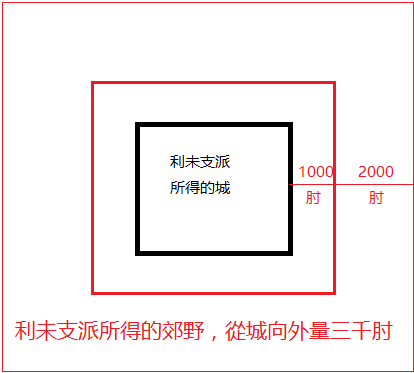
\includegraphics[width=.45\textwidth]{AMoXiFigs/minshuji/liwei}
\caption{利未支派得城的原則}
\end{center}
\end{figure} 
耶和華在摩押平原約旦河邊，耶利哥對面，曉諭摩西說：「你吩咐以色列人，要從所得為業的地中把些城給利未人居住，也要把這城四圍的郊野給利未人。這城邑要歸他們居住，城邑的郊野可以牧養他們的牛羊和各樣的牲畜，又可以安置他們的財物。你們給利未人的郊野，要從城根起，四圍往外量一千肘。另外東量二千肘、南量二千肘、西量二千肘、北量二千肘為邊界，城在當中。這要歸他們做城邑的郊野。你們給利未人的城邑，其中當有六座逃城，使誤殺人的可以逃到那裡，此外還要給他們四十二座城。你們要給利未人的城，共有四十八座，連城帶郊野都要給他們。以色列人所得的地業從中要把些城邑給利未人。人多的就多給，人少的就少給。各支派要按所承受為業之地把城邑給利未人。」


\subsubsection{設立逃城  35:9-15} 
耶和華曉諭摩西說：「你吩咐以色列人說：你們過約旦河，進了迦南地，就要分出幾座城，為你們做逃城，使誤殺人的可以逃到那裡。這些城可以做逃避報仇人的城，使誤殺人的不至於死，等他站在會眾面前聽審判。你們所分出來的城，要做六座逃城。在\textcolor{blue}{約旦河東}要分出三座城，在\textcolor{blue}{迦南地}也要分出三座城，都做逃城。這六座城要給\textcolor{blue}{以色列人}和他們\textcolor{blue}{中間的外人}，並\textcolor{blue}{寄居的}，作為逃城，使誤殺人的都可以逃到那裡。

\subsubsection{故殺人的逃城不能庇护 35:16-21} 
\begin{itemize} 
\itemsep-.35em
\item 若人\textcolor{blue}{用鐵器打人}，以致打死，他就是故殺人的，故殺人的必被治死。 
\item 若\textcolor{blue}{用可以打死人的石頭}打死了人，他就是故殺人的，故殺人的必被治死。 
\item 若\textcolor{blue}{用可以打死人的木器}打死了人，他就是故殺人的，故殺人的必被治死。報血仇的必親自殺那故殺人的，一遇見就殺他。 
\item 人若因\textcolor{blue}{怨恨把人推倒}，或是\textcolor{blue}{埋伏往人身上扔物}以至於死
\item 或是\textcolor{blue}{因仇恨用手打人}以至於死，那打人的必被治死。他是故殺人的，報血仇的一遇見就殺他。
\end{itemize}

\subsubsection{逃城的庇护原则  35:22-28} 
倘若人沒有仇恨，忽然將人推倒，或是沒有埋伏把物扔在人身上，或是沒有看見的時候用可以打死人的石頭扔在人身上，以至於死，本來與他無仇，也無意害他，會眾就要照典章，在打死人的和報血仇的中間審判。會眾要救這誤殺人的脫離報血仇人的手，也要使他歸入逃城。\\
他要住在其中，直等到受聖膏的大祭司死了。但誤殺人的，無論什麼時候，若出了逃城的境外，報血仇的在逃城境外遇見他，將他殺了，報血仇的就沒有流血之罪。 因為誤殺人的該住在逃城裡，等到大祭司死了。大祭司死了以後，誤殺人的才可以回到他所得為業之地。

\subsubsection{故殺人犯死罪的必被治死  35:29-34} 
「這在你們一切的住處，要做你們世世代代的律例、典章。無論誰故殺人，要憑幾個見證人的口把那故殺人的殺了，只是不可憑一個見證的口叫人死。故殺人，犯死罪的，你們\textcolor{red}{不可收贖價代替他的命}，他必被治死。那逃到逃城的人，你們不可為他收贖價，使他在大祭司未死以先再來住在本地。這樣，你們就不汙穢所住之地，因為血是汙穢地的。若有在地上流人血的，非流那殺人者的血，那地就不得潔淨(贖)。你們不可玷汙所住之地，就是我住在其中之地，因為我耶和華住在以色列人中間。」
 	
 	
\subsection{女子承地為業的條例 36 }
\subsubsection{瑪拿西族長在摩西和首領面前的诉求 36:1-4}
約瑟的後裔，瑪拿西的孫子、瑪吉的兒子基列，他子孫中的諸族長來到摩西和做首領的以色列人族長面前，說：「耶和華曾吩咐我主拈鬮分地給以色列人為業，我主也受了耶和華的吩咐將我們兄弟西羅非哈的產業分給他的眾女兒。她們若嫁以色列別支派的人，就必將我們祖宗所遺留的產業加在她們丈夫支派的產業中。這樣，我們拈鬮所得的產業就要減少了。到了以色列人的禧年，這女兒的產業就必加在她們丈夫支派的產業上。這樣，我們祖宗支派的產業就減少了。」
 
\subsubsection{得業女子必嫁同宗支派的人 36:5-9}
摩西照耶和華的話吩咐以色列人說：「約瑟支派的人說得有理。論到西羅非哈的眾女兒，耶和華這樣吩咐說：她們可以隨意嫁人，只是要嫁同宗支派的人。這樣，以色列人的產業就不從這支派歸到那支派，因為以色列人要各守各祖宗支派的產業。凡在以色列支派中得了產業的女子，必做同宗支派人的妻，好叫以色列人各自承受他祖宗的產業。這樣，他們的產業就不從這支派歸到那支派，因為以色列支派的人要各守各的產業。」

\subsubsection{西羅非哈的五女都嫁入瑪拿西子孫 36:10-12}
耶和華怎樣吩咐摩西，西羅非哈的眾女兒就怎樣行。西羅非哈的女兒瑪拉、得撒、曷拉、密迦、挪阿都嫁了她們伯叔的兒子。她們嫁入約瑟兒子瑪拿西子孫的族中，她們的產業仍留在同宗支派中。這是耶和華在摩押平原約旦河邊，耶利哥對面藉著摩西所吩咐以色列人的命令、典章。



\include{AMoXiFiles/ShenMingJi}
\iffalse
\include{AMoXiFiles/ZongJieChuangShiJi}
\include{AMoXiFiles/ChuangShiJiWenTi}
\include{AMoXiFiles/ChuangShiJiZongJie}
\fi

\iffalse
\include{AMoXiFiles/ChuangShiJi}
\include{AMoXiFiles/ZongJieChuangShiJi}
%\vspace{-10 cm}
\chapter{出埃及}
\vspace{-1 cm}
\section{神預備摩西 1-4 }
\subsection{摩西出生 1:1-2:10}
\noindent
\subsubsection{以色列人生養眾多,被埃及新王苦害 1:1-14}
以色列的眾子各帶家眷和雅各一同來到埃及，他們的名字記在下面。 2 有魯本、西緬、利未、猶大、 3 以薩迦、西布倫、便雅憫、 4 但、拿弗他利、迦得、亞設。 5 凡從雅各而生的，共有七十人。約瑟已經在埃及。 6 約瑟和他的弟兄，並那一代的人都死了。 7 以色列人生養眾多，並且繁茂，極其強盛，滿了那地。

%\subsubsection{埃及新王苦害以色列 1:8-14}
有不認識約瑟的新王起來，治理埃及， 9 對他的百姓說：「看哪，這以色列民比我們還多，又比我們強盛。 10 來吧，我們不如用巧計待他們，恐怕他們多起來，日後若遇什麼爭戰的事，就聯合我們的仇敵攻擊我們，離開這地去了。」 11 於是埃及人派督工的轄制他們，加重擔苦害他們。他們為法老建造兩座積貨城，就是比東和蘭塞。 12 只是越發苦害他們，他們越發多起來，越發蔓延，埃及人就因以色列人愁煩。 13 埃及人嚴嚴地使以色列人做工， 14 使他們因做苦工覺得命苦。無論是和泥，是做磚，是做田間各樣的工，在一切的工上都嚴嚴地待他們。

\subsubsection{收生婆存留男孩的性命 1:15-22}
\noindent
有希伯來的兩個收生婆，一名施弗拉，一名普阿。埃及王對她們說： 16 「你們為希伯來婦人收生，看她們臨盆的時候，若是男孩，就把他殺了，若是女孩，就留她存活。」 17 但是收生婆敬畏神，不照埃及王的吩咐行，竟存留男孩的性命。 18 埃及王召了收生婆來，說：「你們為什麼做這事，存留男孩的性命呢？」 19 收生婆對法老說：「因為希伯來婦人與埃及婦人不同，希伯來婦人本是健壯的(活潑的)，收生婆還沒有到，她們已經生產了。」 20 神厚待收生婆。以色列人多起來，極其強盛。 21 收生婆因為敬畏神，神便叫她們成立家室。 22 法老吩咐他的眾民說：「以色列人所生的男孩，你們都要丟在河裡；一切的女孩，你們要存留她的性命。」

\subsubsection{摩西出生 2:1-10}

\begin{table}[H]
\centering
\begin{tabular}{p{9.5cm}|p{7.0cm}}\hline\hline
\multicolumn{1}{c|}{利未母親和姐姐}&\multicolumn{1}{c}{法老的女兒}\\\hline
有一個利未家的人娶了一個利未女子為妻。那女人懷孕，生一個兒子，見他俊美，就藏了他三個月。後來不能再藏，就取了一個蒲草箱，抹上石漆和石油，將孩子放在裡頭，把箱子擱在河邊的蘆荻中。孩子的姐姐遠遠站著，要知道他究竟怎麼樣。&法老的女兒來到河邊洗澡，她的使女們在河邊行走。她看見箱子在蘆荻中，就打發一個婢女拿來。她打開箱子，看見那孩子。孩子哭了，她就可憐他，說：「這是希伯來人的一個孩子。」 \\\hline
孩子的姐姐對法老的女兒說：「我去在希伯來婦人中叫一個奶媽來，為你奶這孩子，可以不可以？」&法老的女兒說：「可以。」\\\hline
童女就去叫了孩子的母親來。&法老的女兒對她說：「你把這孩子抱去，為我奶他，我必給你工價。」\\\hline
婦人就抱了孩子去奶他。孩子漸長，婦人把他帶到法老的女兒那裡，就做了她的兒子。&她給孩子起名叫摩西，意思說：「因我把他從水裡拉出來。」\\\hline
\end{tabular}
\end{table}

\iffalse
\begin{table}[H]
\begin{threeparttable}
\begin{tabular}{@{}p{0.55\textwidth}*{4}{L{\dimexpr0.56\linewidth-10\tabcolsep\relax}}@{}}\toprule
孩子的利未母親和姐姐 &法老的女兒 \\\hline
有一個利未家的人娶了一個利未女子為妻。那女人懷孕，生一個兒子，見他俊美，就藏了他三個月。後來不能再藏，就取了一個蒲草箱，抹上石漆和石油，將孩子放在裡頭，把箱子擱在河邊的蘆荻中。孩子的姐姐遠遠站著，要知道他究竟怎麼樣。&法老的女兒來到河邊洗澡，她的使女們在河邊行走。她看見箱子在蘆荻中，就打發一個婢女拿來。她打開箱子，看見那孩子。孩子哭了，她就可憐他，說：「這是希伯來人的一個孩子。」  \tabularnewline \hline
孩子的姐姐對法老的女兒說：「我去在希伯來婦人中叫一個奶媽來，為你奶這孩子，可以不可以？」&法老的女兒說：「可以。」 \tabularnewline \hline
童女就去叫了孩子的母親來。&法老的女兒對她說：「你把這孩子抱去，為我奶他，我必給你工價。」．\tabularnewline \hline
婦人就抱了孩子去奶他。孩子漸長，婦人把他帶到法老的女兒那裡，就做了她的兒子。&她給孩子起名叫摩西，意思說：「因我把他從水裡拉出來。」\tabularnewline \hline
\bottomrule
\end{tabular}
%\end{tabularx}
%\caption{摩西出生}
\end{threeparttable}
\end{table} 
\fi

\subsection{摩西逃往米甸 2:11-2:25}
\subsubsection{摩西殺埃及人逃往米甸 2:11-15}
後來，摩西長大，他出去到他弟兄那裡，看他們的重擔，見一個埃及人打希伯來人的一個弟兄。 12 他左右觀看，見沒有人，就把埃及人打死了，藏在沙土裡。 13 第二天他出去，見有兩個希伯來人爭鬥，就對那欺負人的說：「你為什麼打你同族的人呢？」 14 那人說：「誰立你做我們的首領和審判官呢？難道你要殺我，像殺那埃及人嗎？」摩西便懼怕，說：「這事必是被人知道了。」 15 法老聽見這事，就想殺摩西，但摩西躲避法老，逃往米甸地居住。

\subsubsection{摩西娶西坡拉 2:16-22}
\noindent
一日，他在井旁坐下。米甸的祭司有七個女兒，她們來打水，打滿了槽，要飲父親的群羊。 17 有牧羊的人來把她們趕走了，摩西卻起來幫助她們，又飲了她們的群羊。 18 她們來到父親流珥那裡，他說：「今日你們為何來得這麼快呢？」 19 她們說：「有一個埃及人救我們脫離牧羊人的手，並且為我們打水飲了群羊。」 20 他對女兒們說：「那個人在哪裡？你們為什麼撇下他呢？你們去請他來吃飯。」 21 摩西甘心和那人同住，那人把他的女兒西坡拉給摩西為妻。 22 西坡拉生了一個兒子，摩西給他起名叫革舜，意思說：「因我在外邦做了寄居的。」

\subsubsection{以色列人哀求神 2:23-25 }
過了多年，埃及王死了。以色列人因做苦工，就嘆息哀求，他們的哀聲達於神。 24 神聽見他們的哀聲，就記念他與亞伯拉罕、以撒、雅各所立的約。 25 神看顧以色列人，也知道他們的苦情。

\subsection{摩西遇見神 3:1-4:17 }
\subsubsection{摩西遇見神 3:1-6}
\begin{table}[H]
\centering
\begin{tabular}{p{7.5cm}|p{9.50cm}}\hline\hline
\multicolumn{1}{c|}{摩西}&\multicolumn{1}{c}{神}\\\hline
摩西牧養他岳父米甸祭司葉忒羅的羊群，一日領羊群往野外去，到了神的山，就是何烈山 & 耶和華的使者從荊棘裡火焰中向摩西顯現,摩西觀看，不料，荊棘被火燒著，卻沒有燒毀\\\hline
我要過去看這大異象、這荊棘為何沒有燒壞呢 &耶和華神見他過去要看，就從荊棘裡呼叫說： 摩西、摩西\\\hline
我在這裡&不要近前來,當把你腳上的鞋脫下來.因為你所站之地是聖地．我是你父親的神、是亞伯拉罕的神、以撒的神、雅各的神。\\\hline
摩西蒙上臉、因為怕看神。&\\\hline
\end{tabular}
\end{table}



%\vspace{-0.8 cm}
\subsubsection{遣摩西領以色列人出埃及 3:7-22}
\begin{table}[H]
\begin{threeparttable}
\begin{tabular}{@{}p{0.23\textwidth}*{4}{L{\dimexpr0.9\linewidth-10\tabcolsep\relax}}@{}}
\toprule
摩西 &  神 \\\hline
&耶和華說：我的百姓在埃及所受的困苦、我實在看見了．他們因受督工的轄制所發的哀聲、我也聽見了．我原知道他們的痛苦。我下來是要救他們脫離埃及人的手、領他們出了那地、到美好寬闊流奶與蜜之地、就是到迦南人、赫人、亞摩利人、比利洗人、希未人、耶布斯人之地。現在以色列人的哀聲達到我耳中、我也看見埃及人怎樣欺壓他們。故此我要打發你去見法老、使你可以將我的百姓以色列人從埃及領出來。\tabularnewline \hline
\vspace{-.6cm}{摩西對神說：「我是什麼人?竟能去見法老,將以色列人從埃及領出來呢?」}&神說：「我必與你同在。你將百姓從埃及領出來之後，你們必在這山上侍奉我，這就是我打發你去的證據。」\tabularnewline \hline
摩西對神說：「我到以色列&神對摩西說：「我是自有永有的。」\tabularnewline
人那裡，對他們說：『你們&又說：「你要對以色列人這樣說：『那自有的打發我到你們這裡來。』」\tabularnewline
\vspace{-3cm}{祖宗的神打發我到你們這裡來。』他們若問我說：『他叫什麼名字？』我要對他們說什麼呢？」}&神又對摩西說：「你要對以色列人這樣說：『耶和華你們祖宗的神，就是亞伯拉罕的神、以撒的神、雅各的神，打發我到你們這裡來。』耶和華是我的名，直到永遠；這也是我的紀念，直到萬代。你去招聚以色列的長老，對他們說：『耶和華你們祖宗的神，就是亞伯拉罕的神、以撒的神、雅各的神，向我顯現，說：我實在眷顧了你們，我也看見埃及人怎樣待你們。』我也說：『要將你們從埃及的困苦中領出來，往迦南人、赫人、亞摩利人、比利洗人、希未人、耶布斯人的地去，就是到流奶與蜜之地。』他們必聽你的話。你和以色列的長老要去見埃及王，對他說：『耶和華希伯來人的神遇見了我們，現在求你容我們往曠野去，走三天的路程，為要祭祀耶和華我們的神。』 我知道雖用大能的手，埃及王也不容你們去。我必伸手在埃及中間施行我一切的奇事，攻擊那地，然後他才容你們去。我必叫你們在埃及人眼前蒙恩，你們去的時候就不至於空手而去。但各婦女必向她的鄰舍並居住在她家裡的女人要金器銀器和衣裳，好給你們的兒女穿戴，這樣你們就把埃及人的財物奪去了。」\tabularnewline
\hline
\bottomrule
\end{tabular}
%\end{tabularx}
%\caption{遣摩西領以色列人出埃及}
\end{threeparttable}
\end{table} 


\subsubsection{杖變蛇,手生大痲瘋為證 4:1-9}
\begin{table}[H]
%\vspace{-.5 cm}
\begin{threeparttable}
\begin{tabular}{@{}p{0.4\textwidth}*{4}{L{\dimexpr0.725\linewidth-10\tabcolsep\relax}}@{}}
\toprule
摩西 &  神 \\\hline
摩西回答說:他們必不信我,也不聽我的話,必說:『耶和華並沒有向你顯現』&耶和華對摩西說：「你手裡是什麼？」\tabularnewline \hline
他說：「是杖。」&耶和華說：「丟在地上。」\tabularnewline\hline
\vspace{-.5cm}{他一丟下去，就變做蛇，摩西便跑開}&耶和華對摩西說:「伸出手來拿住牠的尾巴,牠必在你手中仍變為杖. 如此好叫他們信耶和華他們祖宗的神,就是亞伯拉罕的神,以撒的神,雅各的神是向你顯現了。」耶和華又對他說：「把手放在懷裡。」\tabularnewline\hline
他就把手放在懷裡,及至抽出來,不料手長了大痲瘋,有雪那樣白&耶和華又對他說：「把手放在懷裡。」\tabularnewline\hline
\vspace{-.55cm}{他就再把手放在懷裡，及至從懷裡抽出來，不料，手已經復原，與周身的肉一樣。}
&又說：「倘或他們不聽你的話，也不信頭一個神蹟，他們必信第二個神蹟。這兩個神蹟若都不信，也不聽你的話，你就從河裡取些水，倒在旱地上，你從河裡取的水必在旱地上變做血。」\tabularnewline\hline
\bottomrule
\end{tabular}
%\end{tabularx}
%\caption{手生大痲瘋為證}
\end{threeparttable}
\end{table} 

\subsubsection{摩西拒绝受差遣 4:10-17}
\begin{table}[H]
%\vspace{-.5 cm}
\begin{threeparttable}
\begin{tabular}{@{}p{0.35\textwidth}*{4}{L{\dimexpr0.75\linewidth-10\tabcolsep\relax}}@{}}
\toprule
摩西 &  神 \\\hline
\vspace{-.65cm}{摩西對耶和華說：「主啊，我素日不是能言的人，就是從你對僕人說話以後，也是這樣。我本是拙口笨舌的。」}
&耶和華對他說：「誰造人的口呢？誰使人口啞、耳聾、目明、眼瞎呢？豈不是我耶和華嗎？ 現在去吧，我必賜你口才，指教你所當說的話。」 \tabularnewline\hline
摩西說：「主啊，你願意打發誰，就打發誰去吧！」
&耶和華向摩西發怒說：「不是有你的哥哥利未人亞倫嗎？我知道他是能言的，現在他出來迎接你，他一見你，心裡就歡喜。你要將當說的話傳給他，我也要賜你和他口才，又要指教你們所當行的事。他要替你對百姓說話，你要以他當做口，他要以你當做神。你手裡要拿這杖，好行神蹟。」\tabularnewline
\hline
\bottomrule
\end{tabular}
%\end{tabularx}
%\caption{摩西拒绝受差遣}
\end{threeparttable}
\end{table} 

\subsection{摩西受差返回埃及 4:18-31}
\subsubsection{摩西辞别岳父葉忒羅 4:18}
\begin{wrapfigure}{r}{0.55\textwidth}
\vspace*{-19mm}
-\hspace*{-5mm}
\centering
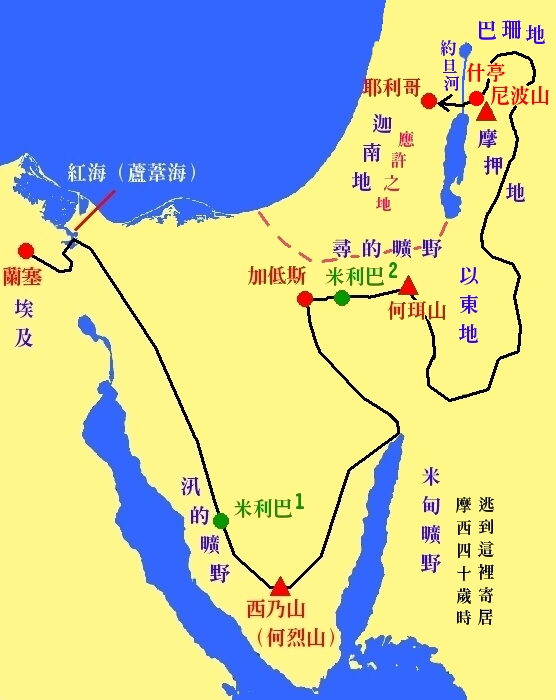
\includegraphics[width=0.8\textwidth]{AMoXiFigs/chuaiji/moses}
%\caption{以色列在曠野的經歷}
\label{fig:sub1}
\end{wrapfigure}
於是，摩西回到他岳父葉忒羅那裡，對他說：「求你容我回去見我在埃及的弟兄，看他們還在不在。」葉忒羅對摩西說：「你可以平平安安地去吧。」

\subsubsection{摩西回埃及的路上遇见神 4:19-26}

耶和華在米甸對摩西說：「你要回埃及去，因為尋索你命的人都死了。」摩西就帶著妻子和兩個兒子，叫他們騎上驢，回埃及地去。摩西手裡拿著神的杖。耶和華對摩西說：「你回到埃及的時候，要留意將我指示你的一切奇事行在法老面前。但我要使(任憑)他的心剛硬，他必不容百姓去。你要對法老說：『耶和華這樣說：以色列是我的兒子，我的長子。我對你說過容我的兒子去，好侍奉我，你還是不肯容他去。看哪，我要殺你的長子。』」摩西在路上住宿的地方，耶和華遇見他，想要殺他。西坡拉就拿一塊火石，割下他兒子的陽皮，丟在摩西腳前，說：「你真是我的血郎了！」 這樣，耶和華才放了他。西坡拉說：「你因割禮就是血郎了。」

\newpage
\subsubsection{亞倫迎接摩西 4:27-31}
耶和華對亞倫說：「你往曠野去迎接摩西。」他就去，在神的山遇見摩西，和他親嘴。 28 摩西將耶和華打發他所說的言語和囑咐他所行的神蹟都告訴了亞倫。 29 摩西、亞倫就去招聚以色列的眾長老。 30 亞倫將耶和華對摩西所說的一切話述說了一遍，又在百姓眼前行了那些神蹟。 31 百姓就信了。以色列人聽見耶和華眷顧他們，鑒察他們的困苦，就低頭下拜。


\section{以色列人出埃及 5-12}
\subsection{摩西亞倫見法老的第一回合 5:1-21}
\subsubsection{摩西亞倫初次見法老 5:1-5}
\begin{itemize} 
\itemsep-.35em 
\item 後來摩西、亞倫去對法老說：「耶和華以色列的神這樣說：『容我的百姓去，在曠野向我守節。』」法老說：「耶和華是誰，使我聽他的話，容以色列人去呢？我不認識耶和華，也不容以色列人去。」
\item 他們說：「希伯來人的神遇見了我們。求你容我們往曠野去，走三天的路程，祭祀耶和華我們的神，免得他用瘟疫、刀兵攻擊我們。」埃及王對他們說：「摩西，亞倫，你們為什麼叫百姓曠工呢？你們去擔你們的擔子吧！」又說：「看哪，這地的以色列人如今眾多，你們竟叫他們歇下擔子！」
\end{itemize}

\subsubsection{以色列人的官長受責罰 5:6-21}
\begin{itemize} 
\itemsep-.35em 
\item 當天，法老吩咐督工的和官長說：「你們不可照常把草給百姓做磚，叫他們自己去撿草。他們素常做磚的數目，你們仍舊向他們要，一點不可減少。因為他們是懶惰的，所以呼求說：『容我們去祭祀我們的神。』你們要把更重的工夫加在這些人身上，叫他們勞碌，不聽虛謊的言語。」
\item 以色列人的官長就來哀求法老說：「為什麼這樣待你的僕人？督工的不把草給僕人，並且對我們說：『做磚吧！』看哪，你僕人挨了打，其實是你百姓的錯。」 但法老說：「你們是懶惰的！你們是懶惰的！所以說：『容我們去祭祀耶和華。』現在你們去做工吧！草是不給你們的，磚卻要如數交納。」以色列人的官長聽說「你們每天做磚的工作一點不可減少」，就知道是遭遇禍患了。
\item 他們離了法老出來，正遇見摩西、亞倫站在對面，就向他們說：「願耶和華鑒察你們，施行判斷！因你們使我們在法老和他臣僕面前有了臭名，把刀遞在他們手中殺我們。」
\end{itemize}

\subsection{摩西亞倫見法老的第二回合 6:1-30}
\subsubsection{神向摩西亞倫確認應許 6:1-8}
\begin{itemize} 
\itemsep-.35em 
\item 耶和華對摩西說:現在你必看見我向法老所行的事,使他因我大能的手容以色列人去,且把他們趕出他的地
\item 神曉諭摩西說：「我是耶和華。我從前向亞伯拉罕、以撒、雅各顯現為全能的神，至於我名耶和華，他們未曾知道。我與他們堅定所立的約，要把他們寄居的迦南地賜給他們。我也聽見以色列人被埃及人苦待的哀聲，我也記念我的約。所以你要對以色列人說：我是耶和華，我要用伸出來的膀臂重重地刑罰埃及人，救贖你們脫離他們的重擔，不做他們的苦工。我要以你們為我的百姓，我也要做你們的神。你們要知道我是耶和華你們的神，是救你們脫離埃及人之重擔的。我起誓應許給亞伯拉罕、以撒、雅各的那地，我要把你們領進去，將那地賜給你們為業。我是耶和華。」
\end{itemize}

\subsubsection{人对神應許的反应 6:9-13}
\begin{itemize} 
\itemsep-.35em 
\item 摩西將這話告訴以色列人，只是他們因苦工愁煩，不肯聽他的話。
\item 耶和華曉諭摩西說： 「你進去對埃及王法老說，要容以色列人出他的地。」 
\item 摩西在耶和華面前說：「以色列人尚且不聽我的話，法老怎肯聽我這拙口笨舌的人呢？」\item 耶和華吩咐摩西、亞倫往以色列人和埃及王法老那裡去，把以色列人從埃及地領出來。
\end{itemize}

%\newpage
\subsubsection{摩西亞倫的家譜 6:14-25}
\begin{forest}
  for tree={
    child anchor=west,
    parent anchor=east,
    grow=east,
    draw,
    anchor=west,
    edge path={
      \noexpand\path[\forestoption{edge}]
        (.child anchor) -| +(-5pt,0) -- +(-5pt,0) |-
        (!u.parent anchor)\forestoption{edge label};
    },
  }
  [以色列
    [流便[哈諾] [法路] [希斯崙] [迦米]]
    [西緬[耶母利] [雅憫][阿轄][雅斤][瑣轄][掃羅（南女子的兒子）]]
    [利未（137歲）[約基別][革順[立尼][示每]] 
    					[哥轄（133歲）[暗蘭（妻子約基別）[亞倫（妻以利沙巴[拿答][亞比戶][以利亞撒[非尼哈]][以他瑪]][摩西][米利暗（姐姐）]
            ]
    									  [以斯哈[可拉[亞惜][以利加拿][亞比亞撒]][尼斐][細基利]]
    									  [希伯倫]
    									  [烏薛[米沙利][以利撒反][西提利]]] 
    					[米拉利[抹利][母示]]]                            
  ]
\end{forest}

\subsubsection{简介摩西亞倫 6:26-27}
\begin{itemize} 
\itemsep-.35em 
\item 亞倫的兒子以利亞撒娶了普鐵的一個女兒為妻，她給他生了非尼哈。這是利未人的家長，都按著他們的家
\item 耶和華說：「將以色列人按著他們的軍隊從埃及地領出來。」這是對那亞倫、摩西說的。對埃及王法老說要將以色列人從埃及領出來的，就是這摩西、亞倫。
\end{itemize}


\subsubsection{摩西亞倫受神命見法老 6:28-7:7}
\begin{itemize} 
\itemsep-.35em 
\item 當耶和華在埃及地對摩西說話的日子, 他向摩西說:我是耶和華，我對你說的一切話你都要告訴埃及王法老
\item 摩西在耶和華面前說：「看哪，我是拙口笨舌的人，法老怎肯聽我呢？」
\item 耶和華對摩西說：「我使你在法老面前代替神，你的哥哥亞倫是替你說話的。凡我所吩咐你的，你都要說。你的哥哥亞倫要對法老說，容以色列人出他的地。我要使法老的心剛硬，也要在埃及地多行神蹟奇事。但法老必不聽你們，我要伸手重重地刑罰埃及，將我的軍隊以色列民從埃及地領出來。我伸手攻擊埃及，將以色列人從他們中間領出來的時候，埃及人就要知道我是耶和華。」
\item 摩西、亞倫這樣行，耶和華怎樣吩咐他們，他們就照樣行了。摩西、亞倫與法老說話的時候，摩西八十歲，亞倫八十三歲
\end{itemize}

\subsubsection{杖變蛇為證 7:8-13}
\begin{itemize} 
\itemsep-.35em 
\item 耶和華曉諭摩西、亞倫說：「法老若對你們說：『你們行件奇事吧』，你就吩咐亞倫說：『把杖丟在法老面前，使杖變做蛇。』」
\item 摩西、亞倫進去見法老，就照耶和華所吩咐的行。亞倫把杖丟在法老和臣僕面前，杖就變做蛇。於是法老召了博士和術士來，他們是埃及行法術的，也用邪術照樣而行。他們各人丟下自己的杖，杖就變做蛇，但\underline{亞倫的杖吞了他們的杖}。
\item 法老心裡剛硬，不肯聽從摩西、亞倫，正如耶和華所說的。
\end{itemize}

\subsection{十災 6:28-12:36}



\subsubsection{水變血之災 7:14-25}
\begin{itemize} 
\itemsep-.35em 
\item 耶和華對摩西說：法老心裡固執，不肯容百姓去。明日早晨，他出來往水邊去，你要往河邊迎接他，手裡要拿著那變過蛇的杖
\begin{itemize} 
\itemsep-.35em 
\item 對他(法老)說：『耶和華希伯來人的神打發我來見你，說：「容我的百姓去，好在曠野侍奉我」，到如今你還是不聽。耶和華這樣說：我要用我手裡的杖擊打河中的水，水就變做血，因此你必知道我是耶和華。河裡的魚必死，河也要腥臭，埃及人就要厭惡吃這河裡的水。』
\item 耶和華曉諭摩西說：「你對亞倫說：『把你的杖伸在埃及所有的水以上，就是在他們的江、河、池、塘以上，叫水都變做血。在埃及遍地，無論在木器中、石器中，都必有血。』」
\end{itemize}
\item 摩西、亞倫就照耶和華所吩咐的行。亞倫在法老和臣僕眼前舉杖擊打河裡的水，河裡的水都變做血了。河裡的魚死了，河也腥臭了，埃及人就不能吃這河裡的水。埃及遍地都有了血。 
\item 埃及行法術的，也用邪術照樣而行。法老心裡剛硬，不肯聽摩西、亞倫，正如耶和華所說的。法老轉身進宮，也不把這事放在心上。埃及人都在河的兩邊挖地，要得水喝，因為他們不能喝這河裡的水。耶和華擊打河以後滿了七天。
\end{itemize}

\subsubsection{蛙災 8:1-15}
耶和華吩咐摩西說：「你進去見法老，對他說：『耶和華這樣說：容我的百姓去，好侍奉我。 2 你若不肯容他們去，我必使青蛙糟蹋你的四境。 3 河裡要滋生青蛙，這青蛙要上來進你的宮殿和你的臥房，上你的床榻，進你臣僕的房屋，上你百姓的身上，進你的爐灶和你的摶麵盆， 4 又要上你和你百姓並你眾臣僕的身上。』」

耶和華曉諭摩西說：「你對亞倫說：『把你的杖伸在江、河、池以上，使青蛙到埃及地上來。』」 6 亞倫便伸杖在埃及的諸水以上，青蛙就上來，遮滿了埃及地。 7 行法術的也用他們的邪術照樣而行，叫青蛙上了埃及地。

8 法老召了摩西、亞倫來，說：「請你們求耶和華，使這青蛙離開我和我的民，我就容百姓去祭祀耶和華。」 9 摩西對法老說：「任憑你吧！我要何時為你和你的臣僕並你的百姓祈求，除滅青蛙離開你和你的宮殿，只留在河裡呢？」 10 他說：「明天。」摩西說：「可以照你的話吧！好叫你知道沒有像耶和華我們神的。 11 青蛙要離開你和你的宮殿，並你的臣僕與你的百姓，只留在河裡。」 12 於是摩西、亞倫離開法老出去。摩西為擾害法老的青蛙呼求耶和華。 13 耶和華就照摩西的話行。凡在房裡、院中、田間的青蛙都死了。 14 眾人把青蛙聚攏成堆，遍地就都腥臭。 15 但法老見災禍鬆緩，就\textcolor{red}{硬著心}，不肯聽他們，正如耶和華所說的。


\subsubsection{蝨災 8:16-19}
耶和華吩咐摩西說：「你對亞倫說：『伸出你的杖擊打地上的塵土，使塵土在埃及遍地變做蝨子(虼蚤)。』」 17 他們就這樣行。亞倫伸杖擊打地上的塵土，就在人身上和牲畜身上有了蝨子，埃及遍地的塵土都變成蝨子了。 18 行法術的也用邪術要生出蝨子來，卻是不能。於是在人身上和牲畜身上都有了蝨子。

\subsubsection{蠅災 8:20-32}
耶和華對摩西說：「你清早起來，法老來到水邊，你站在他面前，對他說：『耶和華這樣說：容我的百姓去，好侍奉我。你若不容我的百姓去，我要叫成群的蒼蠅到你和你臣僕並你百姓的身上，進你的房屋，並且埃及人的房屋和他們所住的地都要滿了成群的蒼蠅。當那日，我必\textcolor{red}{分別}我百姓所住的歌珊地，使那裡沒有成群的蒼蠅，好叫你知道我是天下的耶和華。我要將我的百姓和你的百姓\textcolor{red}{分別}出來。明天必有這神蹟。』」耶和華就這樣行。蒼蠅成了大群，進入法老的宮殿和他臣僕的房屋，埃及遍地就因這成群的蒼蠅敗壞了。

法老召了摩西、亞倫來，說：「你們去，在這地祭祀你們的神吧！」摩西說：「這樣行本不相宜，因為我們要把埃及人所厭惡的祭祀耶和華我們的神。若把埃及人所厭惡的在他們眼前獻為祭，他們豈不拿石頭打死我們嗎？我們要往曠野去，走三天的路程，照著耶和華我們神所要吩咐我們的祭祀他。」法老說：「我容你們去，在曠野祭祀耶和華你們的神，只是不要走得很遠。求你們為我祈禱。」摩西說：「我要出去求耶和華，使成群的蒼蠅明天離開法老和法老的臣僕並法老的百姓，法老卻不可再行詭詐，不容百姓去祭祀耶和華。」 

於是摩西離開法老去求耶和華。 耶和華就照摩西的話行，叫成群的蒼蠅離開法老和他的臣僕並他的百姓，一個也沒有留下。這一次法老又\textcolor{red}{硬著心}，不容百姓去。


\subsubsection{畜疫之災 9:1-7}
耶和華吩咐摩西說：「你進去見法老，對他說：『耶和華希伯來人的神這樣說：容我的百姓去，好侍奉我。 2 你若不肯容他們去，仍舊強留他們， 3 耶和華的手加在你田間的牲畜上，就是在馬、驢、駱駝、牛群、羊群上，必有重重的瘟疫。 4 耶和華要\textcolor{red}{分別}以色列的牲畜和埃及的牲畜，凡屬以色列人的，一樣都不死。』」 5 耶和華就定了時候，說：「明天耶和華必在此地行這事。」 6 第二天，耶和華就行這事。埃及的牲畜幾乎都死了，只是以色列人的牲畜一個都沒有死。 7 法老打發人去看，誰知以色列人的牲畜連一個都沒有死。法老的心卻是\textcolor{red}{固執}，不容百姓去。

\subsubsection{人和牲畜身上起泡的瘡災 9:8-21}
耶和華吩咐摩西、亞倫說：「你們取幾捧爐灰，摩西要在法老面前向天揚起來。 9 這灰要在埃及全地變做塵土，在人身上和牲畜身上成了起泡的瘡。」 10 摩西、亞倫取了爐灰，站在法老面前。摩西向天揚起來，就在人身上和牲畜身上成了起泡的瘡。 11 行法術的在摩西面前站立不住，因為在他們身上和一切埃及人身上都有這瘡。 12 耶和華使法老的\textcolor{red}{心剛硬}，不聽他們，正如耶和華對摩西所說的。

13 耶和華對摩西說：「你清早起來，站在法老面前，對他說：『耶和華希伯來人的神這樣說：容我的百姓去，好侍奉我。 14 因為這一次我要叫一切的災殃臨到你和你臣僕並你百姓的身上，叫你知道在普天下沒有像我的。 15 我若伸手用瘟疫攻擊你和你的百姓，你早就從地上除滅了。 16 其實，我叫你存立，是特要向你顯我的大能，並要使我的名傳遍天下。 17 你還向我的百姓自高，不容他們去嗎？ 18 到明天約在這時候，我必叫重大的冰雹降下，自從埃及開國以來，沒有這樣的冰雹。 19 現在你要打發人把你的牲畜和你田間一切所有的催進來，凡在田間不收回家的，無論是人是牲畜，冰雹必降在他們身上，他們就必死。』」 20 法老的臣僕中，懼怕耶和華這話的，便叫他的奴僕和牲畜跑進家來。 21 但那不把耶和華這話放在心上的，就將他的奴僕和牲畜留在田裡。


\subsubsection{雹災 9:22-35}
耶和華對摩西說：「你向天伸杖，使埃及遍地的人身上和牲畜身上，並田間各樣菜蔬上，都有冰雹。」 23 摩西向天伸杖，耶和華就打雷下雹，有火閃到地上，耶和華下雹在埃及地上。 24 那時，雹與火摻雜，甚是厲害，自從埃及成國以來，遍地沒有這樣的。 25 在埃及遍地，雹擊打了田間所有的人和牲畜，並一切的菜蔬，又打壞田間一切的樹木。 26 唯獨以色列人所住的歌珊地沒有冰雹。
法老打發人召摩西、亞倫來，對他們說：「這一次我犯了罪了。耶和華是公義的，我和我的百姓是邪惡的。 28 這雷轟和冰雹已經夠了。請你們求耶和華，我就容你們去，不再留住你們。」 29 摩西對他說：「我一出城，就要向耶和華舉手禱告，雷必止住，也不再有冰雹，叫你知道全地都是屬耶和華的。 30 至於你和你的臣僕，我知道你們還是不懼怕耶和華神。」 31 那時，麻和大麥被雹擊打，因為大麥已經吐穗，麻也開了花。 32 只是小麥和粗麥沒有被擊打，因為還沒有長成。 33 摩西離了法老出城，向耶和華舉手禱告，雷和雹就止住，雨也不再澆在地上了。 34 法老見雨和雹與雷止住，就越發犯罪，他和他的臣僕都硬著心。 35 法老的\textcolor{red}{心剛硬}，不容以色列人去，正如耶和華藉著摩西所說的。

\subsubsection{蝗蟲之災 10:1-20}
 耶和華對摩西說：「你進去見法老。我使他和他臣僕的心剛硬，為要在他們中間顯我這些神蹟， 2 並要叫你將我向埃及人所做的事，和在他們中間所行的神蹟，傳於你兒子和你孫子的耳中，好叫你們知道我是耶和華。」 3 摩西、亞倫就進去見法老，對他說：「耶和華希伯來人的神這樣說：『你在我面前不肯自卑要到幾時呢？容我的百姓去，好侍奉我。 4 你若不肯容我的百姓去，明天我要使蝗蟲進入你的境內， 5 遮滿地面，甚至看不見地，並且吃那冰雹所剩的和田間所長的一切樹木。 6 你的宮殿和你眾臣僕的房屋，並一切埃及人的房屋，都要被蝗蟲占滿了。自從你祖宗和你祖宗的祖宗在世以來，直到今日，沒有見過這樣的災。』」摩西就轉身離開法老出去。 7 法老的臣僕對法老說：「這人為我們的網羅要到幾時呢？容這些人去侍奉耶和華他們的神吧！埃及已經敗壞了，你還不知道嗎？」 8 於是摩西、亞倫被召回來見法老，法老對他們說：「你們去侍奉耶和華你們的神，但那要去的是誰呢？」 9 摩西說：「我們要和我們老的少的、兒子女兒同去，且把羊群牛群一同帶去，因為我們務要向耶和華守節。」 10 法老對他們說：「我容你們和你們婦人孩子去的時候，耶和華與你們同在吧！你們要謹慎，因為有禍在你們眼前(你們存著惡意)。 11 不可都去，你們這壯年人去侍奉耶和華吧！因為這是你們所求的。」於是把他們從法老面前攆出去。
耶和華對摩西說：「你向埃及地伸杖，使蝗蟲到埃及地上來，吃地上一切的菜蔬，就是冰雹所剩的。」 13 摩西就向埃及地伸杖，那一晝一夜，耶和華使東風颳在埃及地上，到了早晨，東風把蝗蟲颳了來。 14 蝗蟲上來，落在埃及的四境，甚是厲害，以前沒有這樣的，以後也必沒有。 15 因為這蝗蟲遮滿地面，甚至地都黑暗了，又吃地上一切的菜蔬和冰雹所剩樹上的果子。埃及遍地，無論是樹木，是田間的菜蔬，連一點青的也沒有留下。 16 於是法老急忙召了摩西、亞倫來，說：「我得罪耶和華你們的神，又得罪了你們。 17 現在求你，只這一次，饒恕我的罪，求耶和華你們的神，使我脫離這一次的死亡。」 18 摩西就離開法老去求耶和華。 19 耶和華轉了極大的西風，把蝗蟲颳起，吹入紅海，在埃及的四境連一個也沒有留下。 20 但耶和華使法老的\textcolor{red}{心剛硬}，不容以色列人去。


\subsubsection{黑暗之災 10:21-29}
耶和華對摩西說：「你向天伸杖，使埃及地黑暗，這黑暗似乎摸得著。」 22 摩西向天伸杖，埃及遍地就烏黑了三天。 23 三天之久，人不能相見，誰也不敢起來離開本處，唯有以色列人家中都有亮光。 24 法老就召摩西來，說：「你們去侍奉耶和華，只是你們的羊群牛群要留下，你們的婦人孩子可以和你們同去。」 25 摩西說：「你總要把祭物和燔祭牲交給我們，使我們可以祭祀耶和華我們的神。 26 我們的牲畜也要帶去，連一蹄也不留下，因為我們要從其中取出來，侍奉耶和華我們的神。我們未到那裡，還不知道用什麼侍奉耶和華。」 27 但耶和華使法老的\textcolor{red}{心剛硬}，不肯容他們去。 28 法老對摩西說：「你離開我去吧！你要小心，不要再見我的面，因為你見我面的那日，你就必死！」 29 摩西說：「你說得好，我必不再見你的面了。」

\subsubsection{擊殺頭生的長子牲畜之災 11:1-12:30}
\subsubsubsection{以末次之災警告法老 11:1-10}
耶和華對摩西說：「我再使一樣的災殃臨到法老和埃及，然後他必容你們離開這地。他容你們去的時候，總要催逼你們都從這地出去。 2 你要傳於百姓的耳中，叫他們男女各人向鄰舍要金器銀器。」 3 耶和華叫百姓在埃及人眼前蒙恩，並且摩西在埃及地、法老臣僕和百姓的眼中看為極大。

4 摩西說：「耶和華這樣說：『約到半夜，我必出去巡行埃及遍地， 5 凡在埃及地，從坐寶座的法老直到磨子後的婢女所有的長子，以及一切頭生的牲畜，都必死。 6 埃及遍地必有大哀號，從前沒有這樣的，後來也必沒有。 7 至於以色列中，無論是人是牲畜，連狗也不敢向他們搖舌，好叫你們知道耶和華是將埃及人和以色列人分別出來。』 8 你這一切臣僕都要俯伏來見我，說：『求你和跟從你的百姓都出去』，然後我要出去。」於是，摩西氣憤憤地離開法老，出去了。

耶和華對摩西說：「法老必不聽你們，使我的奇事在埃及地多起來。」 10 摩西、亞倫在法老面前行了這一切奇事，耶和華使法老的心剛硬，不容以色列人出離他的地。

\subsubsubsection{定逾越節之禮 12:1-20}
\begin{itemize} 
\itemsep-.35em 
\item 逾越節 12:1-14
\begin{itemize} 
\itemsep-.35em 
\item 耶和華在埃及地曉諭摩西、亞倫說： 你們要以本月為正月，為一年之首。你們吩咐以色列全會眾說：\underline{本月初十日}，各人要按著父家取羊羔，一家一隻。若是一家的人太少，吃不了一隻羊羔，本人就要和他隔壁的鄰舍共取一隻。你們預備羊羔，要按著人數和飯量計算。要無殘疾、一歲的公羊羔，你們或從綿羊裡取，或從山羊裡取，都可以。 
\item 要留到\underline{本月十四日}，在黃昏的時候，以色列全會眾把羊羔宰了。各家要取點血，塗在吃羊羔的房屋左右的門框上和門楣上。當夜要吃羊羔的肉，用火烤了，與無酵餅和苦菜同吃。不可吃生的，斷不可吃水煮的，要帶著頭、腿、五臟，用火烤了吃。不可剩下一點留到早晨，若留到早晨，要用火燒了。你們吃羊羔當腰間束帶，腳上穿鞋，手中拿杖，趕緊地吃。這是耶和華的逾越節。 
\item 因為那夜我要巡行埃及地，把埃及地一切\underline{頭生的，無論是人是牲畜}，都擊殺了，又要敗壞埃及一切的\underline{神}。我是耶和華。這血要在你們所住的房屋上做記號，我一見這血，就越過你們去，我擊殺埃及地頭生的時候，災殃必不臨到你們身上滅你們。你們要記念這日，守為耶和華的節，作為你們世世代代永遠的定例。
\end{itemize}
\item 無酵節 12:15-20
\begin{itemize} 
\itemsep-.35em 
\item 你們要吃無酵餅\underline{七日}。頭一日要把酵從你們各家中除去，因為從頭一日起，到第七日為止，凡吃有酵之餅的，必從以色列中剪除。 
\item 頭一日你們當有聖會，第七日也當有聖會。這\underline{兩日}之內，除了預備各人所要吃的以外，無論何工都不可做。你們要守無酵節，因為我正當這日把你們的軍隊從埃及地領出來。所以你們要守這日，作為世世代代永遠的定例。 
\item 從\underline{正月十四日晚上，直到二十一日晚上}，你們要吃無酵餅。在你們各家中，七日之內不可有酵，因為凡吃有酵之物的，無論是寄居的是本地的，必從以色列的會中剪除。有酵的物，你們都不可吃，在你們一切住處要吃無酵餅。
\end{itemize}
\end{itemize}

\subsubsubsection{摩西吩咐百姓守逾越節之禮 12:21-28}
於是，摩西召了以色列的眾長老來，對他們說：「你們要按著家口取出羊羔，把這逾越節的羊羔宰了。 22 拿一把牛膝草，蘸盆裡的血，打在門楣上和左右的門框上。你們誰也不可出自己的房門，直到早晨。 23 因為耶和華要巡行擊殺埃及人，他看見血在門楣上和左右的門框上，就必越過那門，不容滅命的進你們的房屋，擊殺你們。 24 這例你們要守著，作為你們和你們子孫永遠的定例。 25 日後，你們到了耶和華按著所應許賜給你們的那地，就要守這禮。 26 你們的兒女問你們說：『行這禮是什麼意思？』 27 你們就說：『這是獻給耶和華逾越節的祭，當以色列人在埃及的時候，他擊殺埃及人，越過以色列人的房屋，救了我們各家。』」於是百姓低頭下拜。 28 耶和華怎樣吩咐摩西、亞倫，以色列人就怎樣行。

\subsubsubsection{耶和華擊殺埃及長子之災 12:29-30}
到了半夜，耶和華把埃及地所有的長子，就是從坐寶座的法老，直到被擄囚在監裡之人的長子，以及一切頭生的牲畜，盡都殺了。 30 法老和一切臣僕，並埃及眾人，夜間都起來了。在埃及有大哀號，無一家不死一個人的。

\subsection{以色列人出埃及 12:31-51}
\subsubsection{法老打發以色列人出離埃及 12:31-36}
夜間，法老召了摩西、亞倫來，說：「起來！連你們帶以色列人從我民中出去，依你們所說的去侍奉耶和華吧！ 32 也依你們所說的，連羊群牛群帶著走吧！並要為我祝福。」 33 埃及人催促百姓，打發他們快快出離那地，因為埃及人說：「我們都要死了。」 34 百姓就拿著沒有酵的生麵，把摶麵盆包在衣服中，扛在肩頭上。 35 以色列人照著摩西的話行，向埃及人要金器銀器和衣裳。 36 耶和華叫百姓在埃及人眼前蒙恩，以致埃及人給他們所要的。他們就把埃及人的財物奪去了。


\subsubsection{以色列人離開埃及 12:37-42}
以色列人從蘭塞起行，往疏割去，除了婦人孩子，步行的男人約有六十萬。 38 又有許多閒雜人，並有羊群牛群，和他們一同上去。 39 他們用埃及帶出來的生麵烤成無酵餅，這生麵原沒有發起，因為他們被催逼離開埃及，不能耽延，也沒有為自己預備什麼食物。 40 以色列人住在埃及共有四百三十年。 41 正滿了四百三十年的那一天，耶和華的軍隊都從埃及地出來了。 42 這夜是耶和華的夜，因耶和華領他們出了埃及地，所以當向耶和華謹守，是以色列眾人世世代代該謹守的。


\subsubsection{申明逾越節例 12:43-51}
耶和華對摩西、亞倫說：「逾越節的例是這樣：外邦人都不可吃這羊羔， 44 但各人用銀子買的奴僕，既受了割禮就可以吃。 45 寄居的和雇工人都不可吃。 46 應當在一個房子裡吃，不可把一點肉從房子裡帶到外頭去。羊羔的骨頭一根也不可折斷。 47 以色列全會眾都要守這禮。 48 若有外人寄居在你們中間，願向耶和華守逾越節，他所有的男子務要受割禮，然後才容他前來遵守，他也就像本地人一樣。但未受割禮的，都不可吃這羊羔。 49 本地人和寄居在你們中間的外人同歸一例。」 50 耶和華怎樣吩咐摩西、亞倫，以色列眾人就怎樣行了。 51 正當那日，耶和華將以色列人按著他們的\textcolor{red}{軍隊}，從埃及地領出來。


\section{以色列在曠野的經歷 13-18}
\sffamily\begin{tikzpicture}
  % Place all element in a matrix of nodes, called m
  % By default all nodes are rectangles with round corners
  % but some special sytles are defined also
  \matrix (m) [matrix of nodes, 
    column sep=5mm,
    row sep=1cm,
    nodes={draw, % General options for all nodes
      line width=1pt,
      anchor=center, 
      text centered,
      rounded corners,
      minimum width=1.5cm, minimum height=8mm
    }, 
    % Define styles for some special nodes
    right iso/.style={isosceles triangle,scale=0.5,sharp corners, anchor=center, xshift=-4mm},
    left iso/.style={right iso, rotate=180, xshift=-8mm},
    txt/.style={text width=1.5cm,anchor=center},
    ellip/.style={ellipse,scale=0.5},
    empty/.style={draw=none}
    ]   
  {
  % Second row of symbols
  % m-1-1
    蘭塞 
  & % m-1-2
    疏割
  & % m-1-3
    以倘   
   & % m-1-4
    比哈希錄  
   & % m-1-5
    |[draw=orange!80!white, ultra thick]| \textbf{密奪}   
   & % m-1-6
    |[coordinate, xshift=-1cm]|  
  \\  
  % Third row of symbols
    % m-2-1  
   瑪撒（探米）或叫米利巴（爭鬧）
  & % m-2-2試探
    |[draw=orange!80!white, ultra thick]| \textbf{汛的曠野} 
  & % m-2-3    
    以琳 
  & % m-2-4  
        |[draw=orange!80!white, ultra thick]| \textbf{瑪拉}       
  & % m-2-5  
    書珥曠野  
  & % m-2-6  (no symbol here, only a point to draw the path)
    |[coordinate, xshift=-1cm]| 
  \\  
利非訂
  & % m-3-1試探
  |[draw=orange!80!white, ultra thick]| \textbf{西乃曠野} 
  & % m-3-1試探
     |[coordinate, xshift=-1cm]| 
      \\     
  };  % End of matrix

  % Now, connect all nodes in a chain.
  % The names of the nodes are automatically generated in the previous matrix. Since the
  % matrix was named ``m'', all nodes have the name m-row-column
  { [start chain,every on chain/.style={join}, every join/.style={line width=1pt}]
    %\chainin (m-1-1);
  	 \chainin (m-1-1);
    \chainin (m-1-2);
    \chainin (m-1-3); 
    \chainin (m-1-4); 
    \chainin (m-1-5); 
    \path (m-1-5) edge node [below] {\small{3天}} (m-2-5) ; 
    \chainin (m-2-5);     
    \chainin (m-2-4);
    \chainin (m-2-3); 
    \chainin (m-2-2);  
    \chainin (m-2-1);  
   \chainin (m-3-1); 
       \path (m-3-1) edge node [below] {\small{葉忒羅}} (m-3-2) ;  
     \chainin (m-3-2);             
    };

                rotate=-90, minimum height=7mm, minimum width=1.3cm, 
                single arrow head extend=1.2mm, single arrow tip angle=120] {};
 
  % Define the style for the blue dotted boxes
  \tikzset{white dotted/.style={draw=white!50!white, line width=1pt,
                               dash pattern=on 1pt off 4pt on 6pt off 4pt,
                                inner sep=4mm, rectangle, rounded corners}};

  % Finally the blue dotted boxes are drawn as nodes fitted to other nodes
 % \node (first dotted box) [blue dotted, 
  %                          fit = (MOD text) (m-2-1) (m-2-4)] {};
  \node (second dotted box) [white dotted,
                            fit = (m-3-2)] {};
  \node at (second dotted box.south) [above, inner sep=1.mm] { \small{頒布律法，建會幕}};
  
  \node (second dotted box) [white dotted,
                            fit = (m-2-1)] {};
  \node at (second dotted box.south) [above, inner sep=1.mm] { \small{摩西擊打磐石}};

   \node (second dotted box) [white dotted,
                            fit = (m-3-1)] {};
  \node at (second dotted box.south) [above, inner sep=1.mm] { \small{與亞瑪力爭戰}};
 
  \node (second dotted box) [white dotted,
                            fit = (m-2-4)] {};
  \node at (second dotted box.south) [above, inner sep=1.mm] { \small{苦水變甜}};

  \node (second dotted box) [white dotted,
                            fit = (m-2-2)] {};
  \node at (second dotted box.south) [above, inner sep=1.mm] { \small{降鵪鶉和嗎哪}};


  % Define the style for the blue dotted boxes
  \tikzset{blue dotted/.style={draw=blue!50!white, line width=1pt,
                               dash pattern=on 1pt off 4pt on 6pt off 4pt,
                                inner sep=4mm, rectangle, rounded corners}};

  % Finally the blue dotted boxes are drawn as nodes fitted to other nodes
 % \node (first dotted box) [blue dotted, 
  %                          fit = (MOD text) (m-2-1) (m-2-4)] {};
  \node (second dotted box) [blue dotted,
                            fit = (m-1-1) (m-1-2) (m-1-3) (m-1-4) (m-1-5)] {};

  % Since these boxes are nodes, it is easy to put text above or below them                          
  %\node at (first dotted box.north) [above, inner sep=3mm] {\textbf{Transmitter}};
  %\node at (second dotted box.south) [below, inner sep=3mm] { \tiny{過紅海前}};
  \node at (second dotted box.south) [above, inner sep=1.mm] { \small{過紅海前}};

\end{tikzpicture}  

\begin{figure}%{.5\linewidth}
\centering
\includegraphics[width=5in]{AMoXiFigs/chuaiji/Exodus}
%\caption{以色列在曠野的經歷}
\label{fig:sub1}
\end{figure}

\begin{figure}%{.5\linewidth}
\centering
\includegraphics[width=6in]{AMoXiFigs/chuaiji/fig3}
%\caption{以色列在曠野的經歷}
\label{fig:sub1}
\end{figure}

\begin{figure}%{.5\linewidth}
\centering
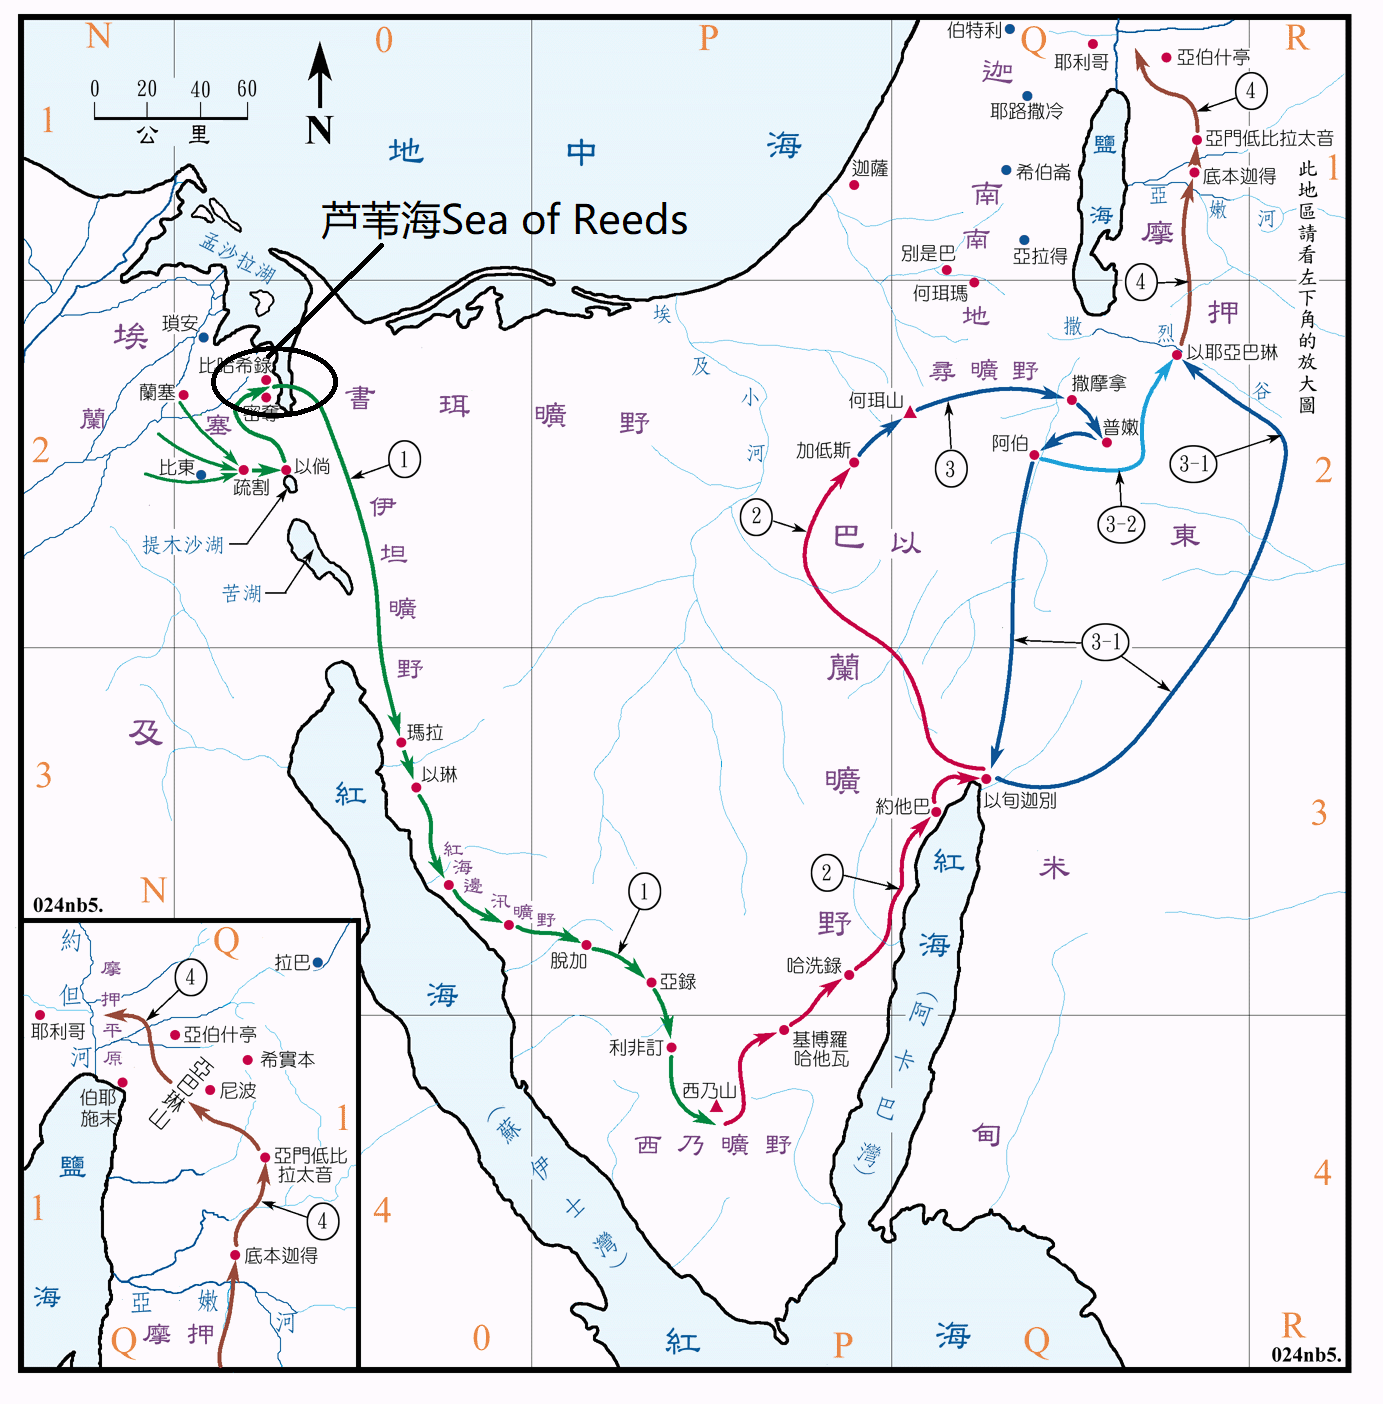
\includegraphics[width=6in]{AMoXiFigs/chuaiji/RedSee1}
%\caption{以色列在曠野的經歷}
\label{fig:sub1}
\end{figure}

\subsection{以色列人摆脱埃及軍隊 13:1-15:21}
\subsubsection{分別頭生 13:1-2(11-16)}
耶和華曉諭摩西說： 2 「以色列中凡頭生的，無論是人是牲畜，都是我的，要分別為聖歸我。」


\subsubsection{亞筆月向耶和華守無酵節七日 13:3-10}
摩西對百姓說：「你們要記念從埃及為奴之家出來的這日，因為耶和華用大能的手將你們從這地方領出來。有酵的餅都不可吃。 4 亞筆月間的這日是你們出來的日子。 5 將來耶和華領你進迦南人、赫人、亞摩利人、希未人、耶布斯人之地，就是他向你的祖宗起誓應許給你那流奶與蜜之地，那時你要在這月間守這禮。 6 你要吃無酵餅七日，到第七日要向耶和華守節。 7 這七日之久，要吃無酵餅，在你四境之內不可見有酵的餅，也不可見發酵的物。 8 當那日，你要告訴你的兒子說：『這是因耶和華在我出埃及的時候為我所行的事。』 9 這要在你手上做記號，在你額上做紀念，使耶和華的律法常在你口中，因為耶和華曾用大能的手將你從埃及領出來。 10 所以你每年要按著日期守這例。

\subsubsection{分別頭生公畜男婴 13:11-16}
將來，耶和華照他向你和你祖宗所起的誓將你領進迦南人之地，把這地賜給你， 12 那時你要將一切頭生的，並牲畜中頭生的，歸給耶和華，公的都要屬耶和華。 13 凡頭生的驢，你要用羊羔代贖，若不代贖，就要打折牠的頸項。凡你兒子中頭生的都要贖出來。 14 日後，你的兒子問你說：『這是什麼意思？』你就說：『耶和華用大能的手將我們從埃及為奴之家領出來。 15 那時法老幾乎不容我們去，耶和華就把埃及地所有頭生的，無論是人是牲畜，都殺了。因此，我把一切頭生的公牲畜獻給耶和華為祭，但將頭生的兒子都贖出來。 16 這要在你手上做記號，在你額上做經文，因為耶和華用大能的手將我們從埃及領出來。』」



\subsubsection{帶約瑟的骸骨繞道紅海曠野，日間雲柱和夜間火柱 13:17-22 }
17 法老容百姓去的時候，非利士地的道路雖近，神卻不領他們從那裡走，因為神說：「恐怕百姓遇見打仗後悔，就回埃及去。」 18 所以神領百姓繞道而行，走紅海曠野的路。以色列人出埃及地，都帶著兵器上去。 19 摩西把約瑟的骸骨一同帶去，因為約瑟曾叫以色列人嚴嚴地起誓，對他們說：「神必眷顧你們，你們要把我的骸骨從這裡一同帶上去。」 20 他們從疏割起行，在曠野邊的以倘安營。 21 日間耶和華在雲柱中領他們的路，夜間在火柱中光照他們，使他們日夜都可以行走。 22 日間雲柱，夜間火柱，總不離開百姓的面前。

%\vspace*{-\baselineskip}
\subsubsection{法老追襲以色列人 14:1-9}
耶和華曉諭摩西說： 2 「你吩咐以色列人轉回，安營在比哈希錄前、密奪和海的中間，對著巴力洗分，靠近海邊安營。 3 法老必說：『以色列人在地中繞迷了，曠野把他們困住了。』 4 我要使法老的心剛硬，他要追趕他們，我便在法老和他全軍身上得榮耀，埃及人就知道我是耶和華。」於是以色列人這樣行了。 5 有人告訴埃及王說：「百姓逃跑！」法老和他的臣僕就向百姓變心，說：「我們容以色列人去，不再服侍我們，這做的是什麼事呢？」 6 法老就預備他的車輛，帶領軍兵同去， 7 並帶著六百輛特選的車和埃及所有的車，每輛都有車兵長。 8 耶和華使埃及王法老的心剛硬，他就追趕以色列人，因為以色列人是昂然無懼地出埃及。 9 埃及人追趕他們，法老一切的馬匹、車輛、馬兵與軍兵就在海邊上，靠近比哈希錄，對著巴力洗分，在他們安營的地方追上了。

\begin{itemize} 
\itemsep-.35em 
\item 耶和華曉諭摩西說：「你\underline{吩咐以色列人轉回}，安營在比哈希錄前、密奪和海的中間，對著巴力洗分，靠近海邊安營。法老必說：『以色列人在地中繞迷了，曠野把他們困住了。』我要使法老的心剛硬，他要追趕他們，我便\underline{在法老和他全軍身上得榮耀，埃及人就知道我是耶和華}。」
\item 於是以色列人這樣行了。有人告訴埃及王說：「百姓逃跑！」法老和他的臣僕就向百姓變心，說：「我們容以色列人去，不再服侍我們，這做的是什麼事呢？」法老就預備他的車輛，帶領軍兵同去，並帶著六百輛特選的車和埃及所有的車，每輛都有車兵長。
\item 耶和華使埃及王法老的心剛硬，他就追趕以色列人，因為以色列人是昂然無懼地出埃及。埃及人追趕他們，法老一切的馬匹、車輛、馬兵與軍兵就在海邊上，靠近比哈希錄，對著巴力洗分，在他們安營的地方追上了。
\end{itemize}

\subsubsection{以色列人懼怕 14:10-14}
法老臨近的時候，以色列人舉目看見埃及人趕來，就甚懼怕，向耶和華哀求。 11 他們對摩西說：「難道在埃及沒有墳地，你把我們帶來死在曠野嗎？你為什麼這樣待我們，將我們從埃及領出來呢？ 12 我們在埃及豈沒有對你說過，不要攪擾我們，容我們服侍埃及人嗎？因為服侍埃及人比死在曠野還好。」 13 摩西對百姓說：「不要懼怕，只管站住，看耶和華今天向你們所要施行的救恩。因為你們今天所看見的埃及人，必永遠不再看見了。 14 耶和華必為你們爭戰，你們只管靜默，不要作聲。」

\begin{itemize} 
\itemsep-.35em 
\item 法老臨近的時候，以色列人舉目看見埃及人趕來，就甚懼怕，向耶和華哀求。他們對摩西說：「難道在埃及沒有墳地，你把我們帶來死在曠野嗎？你為什麼這樣待我們，將我們從埃及領出來呢？我們在埃及豈沒有對你說過，不要攪擾我們，容我們服侍埃及人嗎？因為服侍埃及人比死在曠野還好。」 
\item \underline{摩西對百姓說：「不要懼怕}，只管站住，看耶和華今天向你們所要施行的救恩。因為你們今天所看見的埃及人，必永遠不再看見了。耶和華必為你們爭戰，你們只管靜默，不要作聲。」
\end{itemize}

\subsubsection{紅海邊的雲柱拦阻埃及人 14:15-20}
耶和華對摩西說：「你為什麼向我哀求呢？你吩咐以色列人往前走。 16 你舉手向海伸杖，把水分開，以色列人要下海中走乾地。 17 我要使埃及人的心剛硬，他們就跟著下去，我要在法老和他的全軍、車輛、馬兵上得榮耀。 18 我在法老和他的車輛、馬兵上得榮耀的時候，埃及人就知道我是耶和華了。」 19 在以色列營前行走神的使者，轉到他們後邊去，雲柱也從他們前邊轉到他們後邊立住。 20 在埃及營和以色列營中間有雲柱，一邊黑暗，一邊發光，終夜兩下不得相近。

\begin{itemize} 
\itemsep-.35em 
\item 耶和華對摩西說：「你為什麼向我哀求呢？你吩咐以色列人往前走。你舉手向海伸杖，把水分開，以色列人要下海中走乾地。我要使埃及人的心剛硬，他們就跟著下去，我要在法老和他的全軍、車輛、馬兵上得榮耀。我在法老和他的車輛、馬兵上得榮耀的時候，埃及人就知道我是耶和華了。」 
\item 在以色列營前行走神的使者，轉到他們後邊去，雲柱也從他們前邊轉到他們後邊立住。在埃及營和以色列營中間有雲柱，一邊黑暗，一邊發光，終夜兩下不得相近
\end{itemize}

\subsubsection{投埃及人於海 14:21-31}
摩西向海伸杖，耶和華便用大東風使海水一夜退去，水便分開，海就成了乾地。 22 以色列人下海中走乾地，水在他們的左右做了牆垣。 23 埃及人追趕他們，法老一切的馬匹、車輛和馬兵都跟著下到海中。 24 到了晨更的時候，耶和華從雲火柱中向埃及的軍兵觀看，使埃及的軍兵混亂了， 25 又使他們的車輪脫落，難以行走，以致埃及人說：「我們從以色列人面前逃跑吧！因耶和華為他們攻擊我們了。」

耶和華對摩西說：「你向海伸杖，叫水仍合在埃及人並他們的車輛、馬兵身上。」 27 摩西就向海伸杖，到了天一亮，海水仍舊復原。埃及人避水逃跑的時候，耶和華把他們推翻在海中， 28 水就回流，淹沒了車輛和馬兵。那些跟著以色列人下海法老的全軍，連一個也沒有剩下。 29 以色列人卻在海中走乾地，水在他們的左右做了牆垣。 30 當日，耶和華這樣拯救以色列人脫離埃及人的手，以色列人看見埃及人的死屍都在海邊了。 31 以色列人看見耶和華向埃及人所行的大事，就敬畏耶和華，又信服他和他的僕人摩西。

\begin{itemize} 
\itemsep-.35em 
\item 摩西向海伸杖，耶和華便用\underline{大東風使海水一夜退去，水便分開，海就成了乾地}。
\begin{itemize} 
\itemsep-.35em 
\item 以色列人下海中走乾地，水在他們的左右做了牆垣。 
\item 埃及人追趕他們，法老一切的馬匹、車輛和馬兵都跟著下到海中。
\item 到了晨更的時候，耶和華\underline{從雲火柱中向埃及的軍兵觀看}，使埃及的軍兵混亂了，又使他們的車輪脫落，難以行走，以致埃及人說：「我們從以色列人面前逃跑吧！因耶和華為他們攻擊我們了。」
\end{itemize}
\item 耶和華對摩西說：「你向海伸杖，叫水仍合在埃及人並他們的車輛、馬兵身上。」摩西就向海伸杖，到了天一亮，\underline{海水仍舊復原}。 
\begin{itemize} 
\itemsep-.35em 
\item 埃及人避水逃跑的時候，耶和華把他們推翻在海中，水就回流，淹沒了車輛和馬兵。那些跟著以色列人下海法老的全軍，連一個也沒有剩下。
\item 以色列人卻在海中走乾地，水在他們的左右做了牆垣。當日，耶和華這樣拯救以色列人脫離埃及人的手,以色列人看見埃及人的死屍都在海邊了。以色列人看見耶和華向埃及人所行的大事，就敬畏耶和華，又信服他和他的僕人摩西。
\end{itemize}
\end{itemize}

\subsubsection{摩西歌頌耶和華 15:1-18}
\begin{itemize} 
\itemsep-.35em 
\item 那時，摩西和以色列人向耶和華\underline{唱歌}說：我要向耶和華歌唱,因他大大戰勝，將馬和騎馬的投在海中。耶和華是我的力量、我的詩歌，也成了我的拯救。這是我的神，我要讚美他；是我父親的神，我要尊崇他。耶和華是戰士，他的名是耶和華。\underline{法老}的車輛、軍兵，耶和華已拋在海中，他特選的軍長都沉於紅海。深水淹沒他們，他們如同石頭墜到深處。 耶和華啊，你的右手施展能力，顯出榮耀；耶和華啊，你的右手摔碎仇敵。你大發威嚴，推翻那些起來攻擊你的；你發出烈怒如火，燒滅他們像燒碎秸一樣。你發鼻中的氣，水便聚起成堆，大水直立如壘，海中的深水凝結。仇敵說：『我要追趕，我要追上；我要分擄物；我要在他們身上稱我的心願；我要拔出刀來，親手殺滅他們。』你叫風一吹，海就把他們淹沒，他們如鉛沉在大水之中。 
\item 耶和華啊，眾神之中誰能像你？誰能像你至聖至榮，可頌可畏，施行奇事？你伸出右手，地便吞滅他們。你憑慈愛領了你所贖的百姓，你憑能力引他們到了你的聖所。\underline{外邦人}聽見就發顫，疼痛抓住\underline{非利士}的居民。那時，\underline{以東}的族長驚惶，\underline{摩押}的英雄被戰兢抓住，\underline{迦南}的居民心都消化了，驚駭恐懼臨到他們。耶和華啊，因你膀臂的大能，他們如石頭寂然不動，等候你的百姓過去，等候你所贖的百姓過去。你要將他們領進去，栽於你產業的山上。耶和華啊，就是你為自己所造的住處；主啊，就是你手所建立的聖所。耶和華必做王，直到永永遠遠。」
\end{itemize}

\subsubsection{米利暗歌頌耶和華 15:19-21}
\begin{itemize} 
\itemsep-.35em
\item 法老的馬匹、車輛和馬兵下到海中，耶和華使海水回流淹沒他們，唯有以色列人在海中走乾地。 
\item 亞倫的姐姐女先知米利暗，手裡拿著鼓，眾婦女也跟她出去拿鼓跳舞。
\item 米利暗應聲說：「你們要歌頌耶和華，因他大大戰勝，將馬和騎馬的投在海中。」
\end{itemize}

\subsection{以色列人在曠野 15:22-18:27}
\subsubsection{在瑪拉因為水苦發怨言,樹使苦水變甜 15:22-26}
\begin{itemize} 
\itemsep-.35em
\item 摩西領以色列人從紅海往前行，到了書珥的曠野，在曠野走了三天，找不著水。到了瑪拉，不能喝那裡的水，因為水苦，所以那地名叫瑪拉。 
\item 百姓就向摩西發怨言，說：「我們喝什麼呢？」摩西呼求耶和華，耶和華指示他一棵樹。他把樹丟在水裡，水就變甜了。
\item 耶和華在那裡為他們定了律例、典章，在那裡試驗他們。又說：「你若留意聽耶和華你神的話，又行我眼中看為正的事，留心聽我的誡命，守我一切的律例，我就不將所加於埃及人的疾病加在你身上，因為我耶和華是醫治你的。」
\end{itemize}

\subsubsection{在以琳遇水泉十二 15:27}
\begin{itemize} 
\itemsep-.35em
\item 他們到了以琳，在那裡有十二股水泉，七十棵棕樹，
\item 他們就在那裡的水邊安營。
\end{itemize}

\subsubsection{汛的曠野因饥饿發怨言 16:1-3}
\begin{itemize} 
\itemsep-.35em
\item 以色列全會眾從以琳起行，在出埃及後第二個月十五日，到了以琳和西奈中間汛的曠野。
\item 以色列全會眾在曠野向摩西、亞倫發怨言，說：「巴不得我們早死在埃及地耶和華的手下，那時我們坐在肉鍋旁邊，吃得飽足。你們將我們領出來，到這曠野，是要叫這全會眾都餓死啊！」
\end{itemize}

\subsubsection{神应许賜鵪鶉和嗎哪 16:4-12}
\begin{itemize} 
\itemsep-.35em
\item 耶和華對摩西說：「我要將糧食從天降給你們。百姓可以出去，每天收每天的份，我好試驗他們遵不遵我的法度。到第六天，他們要把所收進來的預備好了，比每天所收的多一倍。」 摩西、亞倫對以色列眾人說：
\begin{itemize} 
\itemsep-.35em
\item 「到了晚上，你們要知道是耶和華將你們從埃及地領出來的。早晨，你們要看見耶和華的榮耀，因為耶和華聽見你們向他所發的怨言了。我們算什麼，你們竟向我們發怨言呢？」 
\item 摩西又說：「耶和華晚上必給你們肉吃，早晨必給你們食物得飽，因為你們向耶和華發的怨言，他都聽見了。我們算什麼？你們的怨言不是向我們發的，乃是向耶和華發的。」 
\item 摩西對亞倫說：「你告訴以色列全會眾說：『你們就近耶和華面前，因為他已經聽見你們的怨言了。』」 
\end{itemize}
\item 亞倫正對以色列全會眾說話的時候，他們向曠野觀看，不料，耶和華的榮光在雲中顯現。耶和華曉諭摩西說：「我已經聽見以色列人的怨言。你告訴他們說：『到黃昏的時候，你們要吃肉，早晨必有食物得飽，你們就知道我是耶和華你們的神。』」
\end{itemize}

\subsubsection{晚上賜鵪鶉，早晨降嗎哪 16:13-15}
\begin{itemize} 
\itemsep-.35em
\item 到了晚上，有\underline{鵪鶉}飛來，遮滿了營。
\item 早晨，在營四圍的地上有露水。露水上升之後，不料，野地面上有\underline{如白霜的小圓物}。
\item 以色列人看見不知道是什麼，就彼此對問說：「這是什麼呢？」摩西對他們說：「這就是耶和華給你們吃的食物
\end{itemize}

\subsubsection{收取嗎哪之例 16:16-30}
\begin{itemize} 
\itemsep-.35em
\item 耶和華所吩咐的是這樣：你們要按著各人的飯量，為帳篷裡的人按著人數收起來，各拿一俄梅珥。
\begin{itemize} 
\itemsep-.35em
\item 以色列人就這樣行，有多收的，有少收的。及至用俄梅珥量一量，多收的也沒有餘，少收的也沒有缺，各人\underline{按著自己的飯量收取}。 
\item 摩西對他們說：「所收的，\underline{不許什麼人留到早晨}。」然而他們不聽摩西的話，內中有留到早晨的，就生蟲變臭了。摩西便向他們發怒。
\end{itemize}
\item 他們每日早晨，按著各人的飯量收取，\underline{日頭一發熱就消化了}。 22 到\underline{第六天}，他們收了\underline{雙倍的食物}，每人兩俄梅珥。會眾的官長來告訴摩西， 23 摩西對他們說：「耶和華這樣說：『明天是聖安息日，是向耶和華守的聖安息日。你們要烤的就烤了，要煮的就煮了，所剩下的都留到早晨。』」
\item 他們就照摩西的吩咐留到早晨，也不臭，裡頭也沒有蟲子。 25 摩西說：「你們今天吃這個吧，因為今天是向耶和華守的安息日，你們在田野必找不著了。 26 六天可以收取，第七天乃是安息日，那一天必沒有了。」 
\item 第七天，百姓中有人出去收，什麼也找不著。耶和華對摩西說：「你們不肯守我的誡命和律法，要到幾時呢？ 29 你們看，耶和華既將安息日賜給你們，所以第六天他賜給你們兩天的食物，第七天各人要住在自己的地方，不許什麼人出去。」 於是百姓第七天安息了。
\end{itemize}

\subsubsection{嗎哪 16:31-36}
\begin{itemize} 
\itemsep-.35em
\item 這食物，以色列家叫嗎哪，樣子像芫荽子，顏色是白的，滋味如同攙蜜的薄餅。
\item 摩西說：「耶和華所吩咐的是這樣：要將一滿俄梅珥嗎哪留到世世代代，使後人可以看見我當日將你們領出埃及地，在曠野所給你們吃的食物。」摩西對亞倫說：「你拿一個罐子，盛一滿俄梅珥嗎哪，存在耶和華面前，要留到世世代代。」
\item 耶和華怎麼吩咐摩西，亞倫就怎麼行，把嗎哪放在法櫃前存留。以色列人吃嗎哪共四十年，直到進了有人居住之地，就是迦南的境界。（俄梅珥乃伊法十分之一。）
\end{itemize}

\subsubsection{米利巴摩西擊打磐石 17:1-7 (民數記20:1-13)}
\begin{itemize} 
\itemsep-.35em
\item 以色列全會眾都遵耶和華的吩咐，按著站口從汛的曠野往前行，在利非訂安營。
百姓沒有水喝，所以與摩西爭鬧，說：「給我們水喝吧！」摩西對他們說：「你們為什麼與我爭鬧，為什麼試探耶和華呢？」百姓在那裡甚渴，要喝水，就向摩西發怨言，說：「你為什麼將我們從埃及領出來，使我們和我們的兒女並牲畜都渴死呢？」 
\item 摩西就呼求耶和華說：「我向這百姓怎樣行呢？他們幾乎要拿石頭打死我。」耶和華對摩西說：「你手裡拿著你先前擊打河水的杖，帶領以色列的幾個長老，從百姓面前走過去。我必在何烈的磐石那裡，站在你面前。你要擊打磐石，從磐石裡必有水流出來，使百姓可以喝。」
\item 摩西就在以色列的長老眼前這樣行了。 
\begin{itemize} 
\itemsep-.35em
\item 他給那地方起名叫瑪撒 (試探)，
\item 又叫米利巴(爭鬧)，因以色列人爭鬧，又因他們試探耶和華，說：「耶和華是在我們中間不是？」
\end{itemize}
\end{itemize}

\subsubsection{與亞瑪力人爭戰 17:8-16 }
\begin{itemize} 
\itemsep-.35em
\item 那時，亞瑪力人來在利非訂，和以色列人爭戰。摩西對約書亞說：「你為我們選出人來，出去和亞瑪力人爭戰。明天我手裡要拿著神的杖，站在山頂上。」 
\begin{itemize} 
\itemsep-.35em
\item 於是約書亞照著摩西對他所說的話行，和亞瑪力人爭戰。
\item 摩西、亞倫與戶珥都上了山頂。摩西何時舉手，以色列人就得勝；何時垂手，亞瑪力人就得勝。但摩西的手發沉，他們就搬石頭來，放在他以下，他就坐在上面。亞倫與戶珥扶著他的手，一個在這邊，一個在那邊，他的手就穩住，直到日落的時候。
\item 約書亞用刀殺了亞瑪力王和他的百姓。 
\end{itemize}
\item 耶和華對摩西說：「我要將亞瑪力的名號從天下全然塗抹了，你要將這話寫在書上做紀念，又念給約書亞聽。」摩西築了一座壇，起名叫耶和華尼西 (耶和華是我旌旗)，又說：「耶和華已經起了誓，必世世代代和亞瑪力人爭戰。」
\end{itemize}

\subsubsection{摩西的岳父葉忒羅稱頌神 18:1-13 }
\begin{itemize} 
\itemsep-.35em
\item 摩西的岳父米甸祭司葉忒羅，聽見神為摩西和神的百姓以色列所行的一切事，就是耶和華將以色列從埃及領出來的事，便帶著摩西的妻子西坡拉，就是摩西從前打發回去的，又帶著西坡拉的兩個兒子，一個名叫革舜，因為摩西說：「我在外邦做了寄居的」，一個名叫以利以謝，因為他說：「我父親的神幫助了我，救我脫離法老的刀」——摩西的岳父葉忒羅帶著摩西的妻子和兩個兒子來到神的山，就是摩西在曠野安營的地方。
\item 他對摩西說：「我是你岳父葉忒羅，帶著你的妻子和兩個兒子來到你這裡。」摩西迎接他的岳父，向他下拜，與他親嘴，彼此問安，都進了帳篷。摩西將耶和華為以色列的緣故向法老和埃及人所行的一切事，以及路上所遭遇的一切艱難，並耶和華怎樣搭救他們，都述說於他岳父聽。
\item 葉忒羅因耶和華待以色列的一切好處，就是拯救他們脫離埃及人的手，便甚歡喜。
\begin{itemize} 
\itemsep-.35em
\item 葉忒羅說：「耶和華是應當稱頌的！他救了你們脫離埃及人和法老的手，將這百姓從埃及人的手下救出來。我現今在埃及人向這百姓發狂傲的事上得知，耶和華比萬神都大。」
\item 摩西的岳父葉忒羅把燔祭和平安祭獻給神。亞倫和以色列的眾長老都來了，與摩西的岳父在神面前吃飯
\end{itemize}
\end{itemize}

\subsubsection{葉忒羅獻策選立百姓官長 18:13-27 (申命記1:9-18)}
\begin{itemize} 
\itemsep-.35em
\item 第二天，摩西坐著審判百姓，百姓從早到晚都站在摩西的左右。
\begin{itemize} 
\itemsep-.35em
\item 摩西的岳父看見他向百姓所做的一切事，就說：「你向百姓做的是什麼事呢？你為什麼獨自坐著，眾百姓從早到晚都站在你的左右呢？」
\item 摩西對岳父說：「這是因百姓到我這裡來求問神。他們有事的時候就到我這裡來，我便在兩造之間施行審判，我又叫他們知道神的律例和法度。」 
\end{itemize}
\item 摩西的岳父說：「你這做的不好。你和這些百姓必都疲憊，因為這事太重，你獨自一人辦理不了。 現在你要聽我的話，我為你出個主意，願神與你同在。
\begin{itemize} 
\itemsep-.35em
\item 你要替百姓到神面前，將案件奏告神。又要將律例和法度教訓他們，指示他們當行的道、當做的事。
\item 並要從百姓中揀選有才能的人，就是敬畏神、誠實無妄、恨不義之財的人，派他們做千夫長、百夫長、五十夫長、十夫長，管理百姓。叫他們隨時審判百姓，大事都要呈到你這裡，小事他們自己可以審判
\item 這樣，你就輕省些，他們也可以同當此任。你若這樣行，神也這樣吩咐你，你就能受得住，這百姓也都平平安安歸回他們的住處。」 
\end{itemize}
\item 於是，摩西聽從他岳父的話，按著他所說的去行。摩西從以色列人中揀選了有才能的人，立他們為百姓的首領，做千夫長、百夫長、五十夫長、十夫長。他們隨時審判百姓，有難斷的案件就呈到摩西那裡，但各樣小事他們自己審判。此後，摩西讓他的岳父去，他就往本地去了
\end{itemize}

\section{西奈山得律法，建会幕和祭司体制 19-40}
\subsection{摩西一次上山得十誡 19:1-20:21}
\subsubsection{以色列人至西奈山 19:1-15 }
\begin{itemize} 
\itemsep-.35em
\item 以色列人出埃及地以後，滿了三個月的那一天，就來到西奈的曠野。他們離了利非訂，來到西奈的曠野，就在那裡的山下安營。摩西到神那裡，
\begin{table}[H]
\begin{threeparttable}
\begin{tabular}{@{}p{0.65\textwidth}*{4}{L{\dimexpr0.41\linewidth-10\tabcolsep\relax}}@{}}
\toprule
神 &  摩西 \\\hline
耶和華從山上呼喚他說：「你要這樣告訴雅各家，曉諭以色列人說：我向埃及人所行的事，你們都看見了；且看見我如鷹將你們背在翅膀上，帶來歸我。如今你們若實在聽從我的話，遵守我的約，就要在萬民中做屬我的子民，因為全地都是我的。你們要歸我做祭司的國度，為聖潔的國民。這些話你要告訴以色列人。」 &摩西去召了民間的長老來，將耶和華所吩咐他的話都在他們面前陳明。百姓都同聲回答說：「凡耶和華所說的，我們都要遵行。」摩西就將百姓的話回覆耶和華\tabularnewline\hline
耶和華對摩西說：「我要在密雲中臨到你那裡，叫百姓在我與你說話的時候可以聽見，也可以永遠信你了。」&於是，摩西將百姓的話奏告耶和華  \tabularnewline\hline
耶和華又對摩西說：「你往百姓那裡去，叫他們今天、明天自潔，又叫他們洗衣服。到第三天要預備好了，因為第三天耶和華要在眾百姓眼前降臨在西奈山上。你要在山的四圍給百姓定界限，說：『你們當謹慎，不可上山去，也不可摸山的邊界。凡摸這山的，必要治死他——不可用手摸他，必用石頭打死，或用箭射透。無論是人是牲畜，都不得活。到角聲拖長的時候，他們才可到山根來。』」&摩西下山往百姓那裡去，叫他們自潔，他們就洗衣服。他對百姓說：「到第三天要預備好了。不可親近女人。」 \tabularnewline
\hline
\bottomrule
\end{tabular}
\caption{百姓自潔豫備見神}
\end{threeparttable}
\end{table} 
\end{itemize}

\subsubsection{耶和華於火中降臨西奈山 19:16-25}
\begin{itemize} 
\itemsep-.35em
\item 到了第三天早晨
\begin{itemize} 
\itemsep-.35em
\item 在\underline{山上}有雷轟、閃電和密雲，並且角聲甚大
\item \underline{營中}的百姓盡都發顫。摩西率領百姓出營迎接神，都站在山下
\item 西奈\underline{全山}冒煙，因為耶和華在火中降於山上。山的煙氣上騰，如燒窯一般，遍山大大地震動。角聲漸漸地高而又高
\end{itemize}
\item 摩西就說話，神有聲音答應他。耶和華降臨在西奈山頂上，耶和華召摩西上山頂，摩西就上去。
\begin{table}[H]
\begin{threeparttable}
\begin{tabular}{@{}p{0.6\textwidth}*{4}{L{\dimexpr0.45\linewidth-10\tabcolsep\relax}}@{}}
\toprule
神 &  摩西 \\\hline
耶和華對摩西說：「你下去囑咐百姓，不可闖過來到我面前觀看，恐怕他們有多人死亡。又叫親近我的祭司自潔，恐怕我忽然出來擊殺他們。」&摩西對耶和華說：「百姓不能上西奈山，因為你已經囑咐我們說：『要在山的四圍定界限，叫山成聖。』」\tabularnewline\hline
耶和華對他說：「下去吧，你要和亞倫一同上來，只是祭司和百姓不可闖過來上到我面前，恐怕我忽然出來擊殺他們。」&於是摩西下到百姓那裡告訴他們。 \tabularnewline\hline
\hline
\bottomrule
\end{tabular}
\caption{耶和華於火中降臨西奈山}
\end{threeparttable}
\end{table} 
\end{itemize}


\subsubsection{頒布十誡 20:1-17 (申5:6-21)}
\begin{itemize} 
\itemsep-.35em
\item 对神的条例
\begin{itemize} 
\itemsep-.35em
\item 神吩咐這一切的話說：「我是耶和華你的神，曾將你從埃及地為奴之家領出來。除了我以外，你\underline{不可有別的神}
\item \underline{不可為自己雕刻偶像}，也不可做什麼形象彷彿上天、下地和地底下、水中的百物。不可跪拜那些像，也不可侍奉它，因為我耶和華你的神是忌邪的神。恨我的，我必追討他的罪，自父及子，直到三四代；愛我守我誡命的，我必向他們發慈愛，直到千代
\item \underline{不可妄稱耶和華你神的名}，因為妄稱耶和華名的，耶和華必不以他為無罪
\item \underline{當記念安息日}，守為聖日。六日要勞碌做你一切的工，但第七日是向耶和華你神當守的安息日。這一日你和你的兒女、僕婢、牲畜，並你城裡寄居的客旅，無論何工都不可做。因為六日之內，耶和華造天、地、海和其中的萬物，第七日便安息，所以耶和華賜福於安息日，定為聖日
\end{itemize}
\item 对人的条例
\begin{itemize} 
\itemsep-.35em
\item \underline{當}孝敬父母，使你的日子在耶和華你神所賜你的地上得以長久
\item \underline{不可}殺人
\item \underline{不可}姦淫
\item \underline{不可}偷盜
\item \underline{不可}作假見證陷害人
\item \underline{不可}貪戀人的房屋，也不可貪戀人的妻子、僕婢、牛驢並他一切所有的。
\end{itemize}
\end{itemize}


\subsubsection{百姓見神而懼怕 20:18-21 (申命記5:23-27)}
\begin{itemize} 
\itemsep-.35em
\item 眾百姓見雷轟、閃電、角聲、山上冒煙，就都發顫，遠遠地站立，對摩西說：「求你和我們說話，我們必聽；不要神和我們說話，恐怕我們死亡。」 
\item 摩西對百姓說：「不要懼怕，因為神降臨是要試驗你們，叫你們時常敬畏他，不致犯罪。」於是百姓遠遠地站立，摩西就挨近神所在的幽暗之中。
\end{itemize}


\subsection{摩西二次上山得律法 20:22-23:33}
\subsubsection{禁造神像和築（土、石）壇之條例 20:22-26}
\begin{itemize} 
\itemsep-.35em
\item 耶和華對摩西說：「你要向以色列人這樣說：你們自己看見我從天上和你們說話了。你們\underline{不可做什麼神}像與我相配，不可為自己做金銀的神像。
\item 你要為我\underline{築土壇}，在上面以牛羊獻為燔祭和平安祭。凡記下我名的地方，我必到那裡賜福給你。
 \item 你若為我\underline{築一座石壇}，不可用鑿成的石頭，因你在上頭一動家具，就把壇汙穢了。
\item 你上我的壇，\underline{不可用臺階}，免得露出你的下體來。
\end{itemize}


\subsubsection{對待奴僕之例 21:1-11 （申15:12-18/利25:39-55）}
\begin{itemize} 
\itemsep-.35em
\item 男僕：你在百姓面前所要立的典章是這樣：你若買希伯來人做奴僕
\begin{itemize} 
\itemsep-.35em
\item 他必服侍你六年，第七年他可以自由，白白地出去。
\begin{itemize} 
\itemsep-.35em
\item 他若孤身來，就可以孤身去；
\item 他若有妻，他的妻就可以同他出去。
\item 他主人若給他妻子，妻子給他生了兒子或女兒，妻子和兒女要歸主人，他要獨自出去。
\end{itemize}
\item 倘或奴僕明說：『我愛我的主人和我的妻子、兒女，不願意自由出去。』他的主人就要帶他到審判官（神）那裡，又要帶他到門前，靠近門框，用錐子穿他的耳朵，他就永遠服侍主人。
\end{itemize}
\item 女僕：人若賣女兒做婢女，婢女不可像男僕那樣出去。
\begin{itemize} 
\itemsep-.35em
\item 主人選定她歸自己，若不喜歡她，就要許她贖身；主人既然用詭詐待她，就沒有權柄賣給外邦人。
\item 主人若選定她給自己的兒子，就當待她如同女兒。若另娶一個，那女子的吃食、衣服並好合的事，仍不可減少。若不向她行這三樣，她就可以不用錢贖，白白地出去。
\end{itemize}
\end{itemize}

\subsubsection{人傷害人的赔偿條例 21:12-27}
\begin{itemize} 
\itemsep-.35em
\item 人若彼此相爭
\begin{itemize} 
\itemsep-.35em
\item 打人以致打死的，必要把他治死。人若不是埋伏著殺人，乃是神交在他手中，我就設下一個地方，他可以往那裡逃跑。人若任意用詭計殺了他的鄰舍，就是逃到我的壇那裡，也當捉去把他治死。
\item 人若彼此相爭，這個用石頭或是拳頭打那個，尚且不至於死，不過躺臥在床，若再能起來扶杖而出，那打他的可算無罪，但要將他耽誤的工夫用錢賠補，並要將他全然醫好。
\item 人若彼此爭鬥，傷害有孕的婦人，甚至墜胎，隨後卻無別害，那傷害她的總要按婦人的丈夫所要的，照審判官所斷的受罰。若有別害，就要以命償命，以眼還眼，以牙還牙，以手還手，以腳還腳，以烙還烙，以傷還傷，以打還打。
\end{itemize}
\item 拐帶人口，或是把人賣了，或是留在他手下，必要把他治死。
\item 人若与父母相爭
\begin{itemize} 
\itemsep-.35em
\item 打父母的，必要把他治死。
\item 咒罵父母的，必要把他治死。
\end{itemize}
\item 打死打壞奴僕
\begin{itemize} 
\itemsep-.35em
\item 人若用棍子打奴僕或婢女，立時死在他的手下，他必要受刑。若過一兩天才死，就可以不受刑，因為是用錢買的。
\item 人若打壞了他奴僕或是婢女的一隻眼，就要因他的眼放他去得以自由。若打掉了他奴僕或是婢女的一個牙，就要因他的牙放他去得以自由。
\end{itemize}
\end{itemize}

\subsubsection{人傷動物或動物傷人的條例 21:28-36}
\begin{itemize} 
\itemsep-.35em
\item 牛若觸死男人或是女人
\begin{itemize} 
\itemsep-.35em
\item 牛若觸了自由人
\begin{itemize} 
\itemsep-.35em
\item 總要用石頭打死那牛，卻不可吃牠的肉，牛的主人可算無罪。
\item 倘若那牛素來是觸人的，有人報告了牛主，他竟不把牛拴著，以致把男人或是女人觸死，就要用石頭打死那牛，牛主也必治死。
\item 若罰他贖命的價銀，他必照所罰的贖他的命。
\item 牛無論觸了人的兒子或是女兒，必照這例辦理。
\end{itemize}
\item 牛若觸了奴僕或是婢女，必將銀子三十舍客勒給他們的主人，也要用石頭把牛打死。
\end{itemize}
\item 人若敞著井口，或挖井不遮蓋，有牛或驢掉在裡頭，井主要拿錢賠還本主人，死牲畜要歸自己
\item 牛傷牛
\begin{itemize} 
\itemsep-.35em
\item 這人的牛若傷了那人的牛，以至於死，他們要賣了活牛，平分價值，也要平分死牛。 \item 人若知道這牛素來是觸人的，主人竟不把牛拴著，他必要以牛還牛，死牛要歸自己
\end{itemize}
\end{itemize}

\subsubsection{賠償的條例 22:1-17}
\begin{itemize} 
\itemsep-.35em
\item 牲畜造成的损失
\begin{itemize} 
\itemsep-.35em
\item 人若偷牛或羊，無論是宰了是賣了，他就要以五牛賠一牛，四羊賠一羊。
\item 人若遇見賊挖窟窿，把賊打了，以至於死，就不能為他有流血的罪。若太陽已經出來，就為他有流血的罪。
\item 賊若被拿，總要賠還。若他一無所有，就要被賣，頂他所偷的物。若他所偷的，或牛，或驢，或羊，仍在他手下存活，他就要加倍賠還。
\item 人若在田間或在葡萄園裡放牲畜，任憑牲畜上別人的田裡去吃，就必拿自己田間上好的和葡萄園上好的賠還。
\end{itemize}
\item 人为造成的损失
\begin{itemize} 
\itemsep-.35em
\item 若點火焚燒荊棘，以致將別人堆積的禾捆、站著的禾稼或是田園，都燒盡了，那點火的必要賠還。
\item 人若將銀錢或家具交付鄰舍看守，這物從那人的家被偷去，若把賊找到了，賊要加倍賠還。若找不到賊，那家主必就近審判官，要看看他拿了原主的物件沒有。兩個人的案件，無論是為什麼過犯，或是為牛，為驢，為羊，為衣裳，或是為什麼失掉之物，有一人說『這是我的』，兩造就要將案件稟告審判官，審判官定誰有罪，誰就要加倍賠還。
\item 人若將驢，或牛，或羊，或別的牲畜，交付鄰舍看守，牲畜或死，或受傷，或被趕去，無人看見，那看守的人要憑著耶和華起誓，手裡未曾拿鄰舍的物，本主就要罷休，看守的人不必賠還。牲畜若從看守的那裡被偷去，他就要賠還本主。若被野獸撕碎，看守的要帶來當做證據，所撕的不必賠還。
\item 人若向鄰舍借什麼，所借的或受傷，或死，本主沒有同在一處，借的人總要賠還。若本主同在一處，他就不必賠還。若是雇的，也不必賠還，本是為雇價來的。
\item 人若引誘沒有受聘的處女，與她行淫，他總要交出聘禮，娶她為妻。若女子的父親決不肯將女子給他，他就要按處女的聘禮，交出錢來。
\end{itemize}
\end{itemize}

\subsubsection{敬畏神和不可虧負弱者的條例 22:18-31}
\begin{itemize} 
\itemsep-.35em
\item 敬畏神的条例
\begin{itemize} 
\itemsep-.35em
\item 行邪術的女人，不可容她存活。
\item 凡與獸淫合的，總要把他治死。
\item 祭祀別神，不單單祭祀耶和華的，那人必要滅絕。
\item 不可毀謗神，也不可毀謗你百姓的官長。
\item 你要從你莊稼中的穀和酒榨中滴出來的酒拿來獻上，不可遲延。你要將頭生的兒子歸給我。 你牛羊頭生的，也要這樣，七天當跟著母，第八天要歸給我。
\item 你要在我面前為聖潔的人，因此，田間被野獸撕裂牲畜的肉，你們不可吃，要丟給狗吃
\end{itemize}
\item 不可虧負弱者
\begin{itemize} 
\itemsep-.35em
\item 不可虧負寄居的，也不可欺壓他，因為你們在埃及地也做過寄居的。
\item 不可苦待寡婦和孤兒。若是苦待他們一點，他們向我一哀求，我總要聽他們的哀聲，並要發烈怒，用刀殺你們，使你們的妻子為寡婦，兒女為孤兒。
\item 我民中有貧窮人與你同住，你若借錢給他，不可如放債的向他取利。你即或拿鄰舍的衣服做當頭，必在日落以先歸還他。因他只有這一件當蓋頭，是他蓋身的衣服，若是沒有，他拿什麼睡覺呢？他哀求我，我就應允，因為我是有恩惠的。
\end{itemize}
\end{itemize}


\subsubsection{行公义的条例 23:1-9}
\begin{itemize} 
\itemsep-.35em
\item 不可隨夥布散謠言，不可與惡人連手妄作見證。不可隨眾行惡，不可在爭訟的事上隨眾偏行，作見證屈枉正直。也不可在爭訟的事上偏護窮人。
\item 若遇見你仇敵的牛或驢失迷了路，總要牽回來交給他。若看見恨你人的驢壓臥在重馱之下，不可走開，務要和驢主一同抬開重馱。
\item 不可在窮人爭訟的事上屈枉正直。當遠離虛假的事。不可殺無辜和有義的人，因我必不以惡人為義。
\item 不可受賄賂，因為賄賂能叫明眼人變瞎了，又能顛倒義人的話。
\item 不可欺壓寄居的，因為你們在埃及地做過寄居的，知道寄居的心。
\end{itemize}

\subsubsection{安息年，安息日之例 23:10-13(31:12-18/34:21/35:1-3)}
\begin{itemize} 
\itemsep-.35em
\item 六年你要耕種田地，收藏土產，只是第七年要叫地歇息，不耕不種，使你民中的窮人有吃的，他們所剩下的，野獸可以吃。你的葡萄園和橄欖園也要照樣辦理。
\item 六日你要做工，第七日要安息，使牛、驢可以歇息，並使你婢女的兒子和寄居的都可以舒暢。 
\item 凡我對你們說的話，你們要謹守。別神的名，你不可提，也不可從你口中傳說。
\end{itemize}

\subsubsection{除酵節，收割節（七七節），收藏節 23:14-17 (34:18-24)}
\begin{itemize} 
\itemsep-.35em
\item 一年三次，你要向我守節
\begin{itemize} 
\itemsep-.35em
\item 你要守除酵節，照我所吩咐你的，在亞筆月內所定的日期，吃無酵餅七天。誰也不可空手朝見我，因為你是這月出了埃及。
\item 又要守收割節，所收的是你田間所種、勞碌得來初熟之物。
\item 並在年底收藏，要守收藏節
\end{itemize}
一切的男丁要一年三次朝見主耶和華。
\end{itemize}

\subsubsection{當獻初熟之物 23:18-19}
\begin{itemize} 
\itemsep-.35em
\item 不可將我祭牲的血和有酵的餅一同獻上
\item 也不可將我節上祭牲的脂油留到早晨
\item 地裡首先初熟之物要送到耶和華你神的殿
\item 不可用山羊羔母的奶煮山羊羔。
\end{itemize}

\subsubsection{復許導以色列民進迦南 23:20-23}
\begin{itemize} 
\itemsep-.35em
\item 看哪，我差遣使者在你前面，在路上保護你，領你到我所預備的地方去。他是奉我名來的，你們要在他面前謹慎，聽從他的話，不可惹（違背）他，因為他必不赦免你們的過犯。
\item 你若實在聽從他的話，照著我一切所說的去行，我就向你的仇敵做仇敵，向你的敵人做敵人。我的使者要在你前面行，領你到亞摩利人、赫人、比利洗人、迦南人、希未人、耶布斯人那裡去，我必將他們剪除。
\end{itemize}

\subsubsection{不可事奉迦南地人的神 23:21-33}
\begin{itemize} 
\itemsep-.35em
\item 你不可跪拜他們的神，不可侍奉他，也不可效法他們的行為，卻要把神像盡行拆毀，打碎他們的柱像。你們要侍奉耶和華你們的神
\begin{itemize} 
\itemsep-.35em
\item 他必賜福於你的糧與你的水，也必從你們中間除去疾病。你境內必沒有墜胎的、不生產的；我要使你滿了你年日的數目。
\item 凡你所到的地方，我要使那裡的眾民在你面前驚駭擾亂，又要使你一切仇敵轉背逃跑。我要打發黃蜂飛在你前面，把希未人、迦南人、赫人攆出去。我不在一年之內將他們從你面前攆出去，恐怕地成為荒涼，野地的獸多起來害你。我要漸漸地將他們從你面前攆出去，等到你的人數加多，承受那地為業。我要定你的境界，從紅海直到非利士海，又從曠野直到大河。我要將那地的居民交在你手中，你要將他們從你面前攆出去
\end{itemize}
\item 不可和他們並他們的神立約。他們不可住在你的地上，恐怕他們使你得罪我。你若侍奉他們的神，這必成為你的網羅。」
\end{itemize}


\subsection{摩西三次上山得建造会幕和祭司体系的启示 24-31}
\subsubsection{神召摩西及以色列的領袖上山見神 24:1-11}
\begin{itemize} 
\itemsep-.35em
\item 耶和華對摩西說：「你和亞倫、拿答、亞比戶，並以色列長老中的七十人，都要上到我這裡來，遠遠地下拜。唯獨你可以親近耶和華，他們卻不可親近，百姓也不可和你一同上來。」 
\item 摩西下山，將耶和華的命令、典章都述說於百姓聽，眾百姓齊聲說：「耶和華所吩咐的，我們都必遵行。」
\begin{itemize} 
\itemsep-.35em
\item 摩西將耶和華的命令都寫上。清早起來，在山下築一座壇，按以色列十二支派立十二根柱子， \item 又打發以色列人中的少年人去獻燔祭，又向耶和華獻牛為平安祭。摩西將血一半盛在盆中一半灑在壇上
\item 又將約書念給百姓聽，他們說：「耶和華所吩咐的，我們都必遵行。」 
\item 摩西將血灑在百姓身上，說：「你看，這是立約的血，是耶和華按這一切話與你們立約的憑據
\end{itemize}
\item 摩西、亞倫、拿答、亞比戶，並以色列長老中的七十人，都上了山。他們看見以色列的神，他腳下彷彿有平鋪的藍寶石，如同天色明淨。他的手不加害在以色列的尊者身上。他們觀看神，他們又吃又喝
\end{itemize}

\subsubsection{摩西三次上山見神 24:12-18}
\begin{itemize} 
\itemsep-.35em
\item 耶和華對摩西說:你上山到我這裡來住在這裡，我要將石版並我所寫的律法和誡命賜給你，使你可以教訓百姓 
\item 摩西和他的幫手約書亞起來，上了神的山。
\begin{itemize} 
\itemsep-.35em
\item 摩西對長老說：「你們在這裡等著，等到我們再回來。有亞倫、戶珥與你們同在，凡有爭訟的，都可以就近他們去。」 
\item 摩西上山，有雲彩把山遮蓋。耶和華的榮耀停於西奈山，雲彩遮蓋山六天，第七天他從雲中召摩西。耶和華的榮耀在山頂上，在以色列人眼前，形狀如烈火。摩西進入雲中上山，在山上四十晝夜。
\end{itemize}
\end{itemize}


\subsubsection{造聖所奉獻的物 25:1-9 （35:4-9）}
\begin{figure}%{.5\linewidth}
\centering
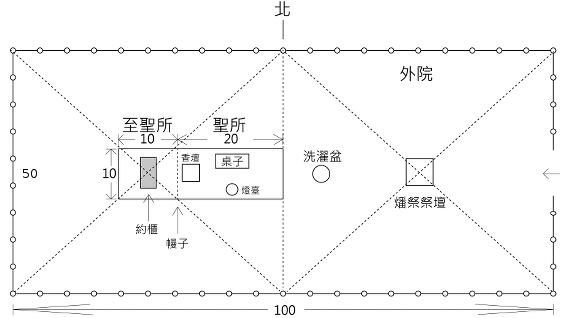
\includegraphics[width=5in]{AMoXiFigs/chuaiji/HuiMu}
%\caption{聖所}
\label{fig:sub1}
\end{figure}
\begin{figure}%{.5\linewidth}
\centering
%
\includegraphics{AMoXiFigs/HuiMuTu.gif}
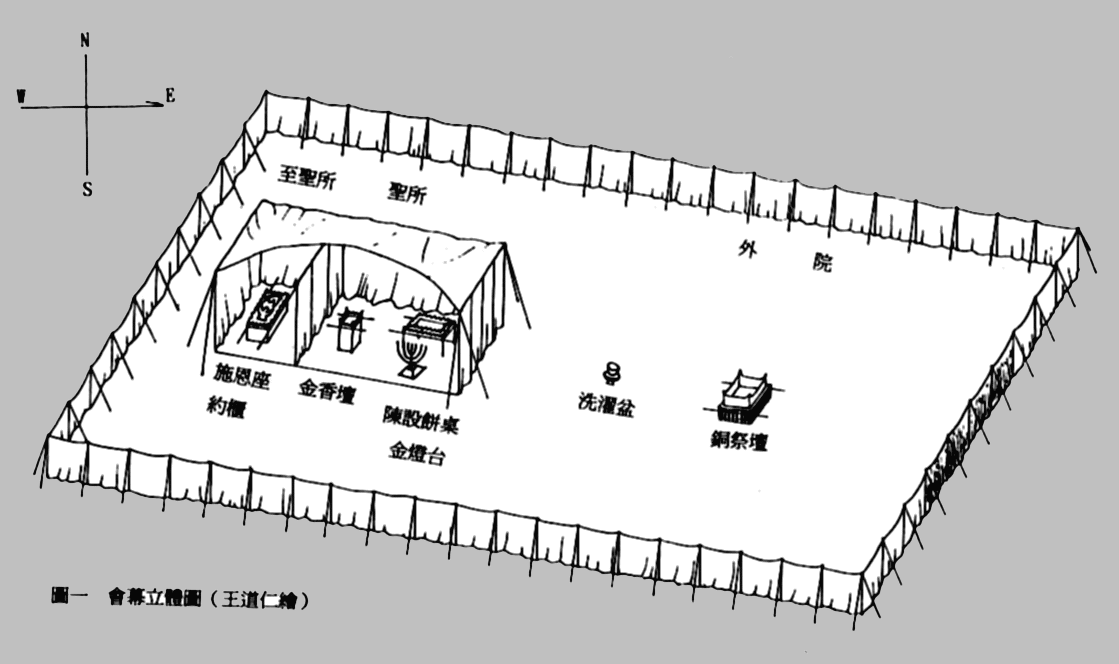
\includegraphics[width=5in]{AMoXiFigs/chuaiji/HuiMuTu}
%\caption{聖所}
\label{fig:sub1}
\end{figure}

\begin{itemize} 
\itemsep-.35em
\item 耶和華曉諭摩西說:你告訴以色列人當為我送禮物來，凡甘心樂意的你們就可以收下歸我。所要收的禮物是
\begin{table}[H]
\centering
\begin{tabular}{|c|c| }
\hline
\hline
材料 & 名稱  \\\hline
金屬 & 金、銀、銅    \\\hline
線類&藍色、紫色、朱紅色線、細麻、山羊毛  \\\hline
皮類&染紅的公羊皮、海狗皮 \\\hline
木類&　皂莢木 　\\\hline
油、香料&點燈的油並做膏油和香的香料　\\\hline
寶石&紅瑪瑙與別樣的寶石，可以鑲嵌在以弗得和胸牌上 \\\hline
\end{tabular}
\caption{奉獻的物}
\end{table}
\item 又當為我造聖所，使我可以住在他們中間。製造帳幕和其中的一切器具，都要照我所指示你的樣式
\end{itemize}

\subsubsection{造約櫃之法則 25:10-22 （37:1-9）}
\begin{itemize} 
\itemsep-.35em
\item 造約櫃之法則
\begin{table}[H]
\centering
\begin{tabular}{|c|l| }
\hline
\hline
部件 & 规格  \\\hline
約櫃 & 皂莢木，長2.5肘 X 寬1.5肘 X 高1.5肘，裡外包上精金、四圍鑲上金牙邊    \\\hline
金環&鑄四個金環安在櫃的四腳上、這邊兩環、那邊兩環。   \\\hline
抬杠&用皂莢木做兩根槓用金包裹。要把槓穿在櫃旁的環內以便抬櫃。這槓要常在櫃的環內，不可抽出來\\\hline
櫃裡&必將我所要賜給你的法版放在櫃裡　\\\hline
施恩座&要用精金做施恩（蔽罪）座，要將施恩座安在櫃的上邊，長2.5肘 X 寬1.5肘　\\\hline
基路伯&要用金子錘出兩個基路伯來，安在施恩座的兩頭。二基路伯要接連一塊。二基路伯要高張翅膀\\
&遮掩施恩座。基路伯要臉對臉，朝著施恩座。要將施恩座安在櫃的上邊  \\\hline
\end{tabular}
\caption{造約櫃之法則}
\end{table}
\item 我要在那裡與你相會，又要從法櫃施恩座上二基路伯中間，和你說我所要吩咐你傳給以色列人的一切事
\end{itemize}

\subsubsection{造陳設餅的桌子及器皿 25:23-30  （37:10-16）}
\begin{table}[H]
\centering
\begin{tabular}{|c|l| }
\hline
\hline
部件 & 规格   \\\hline
桌子 &要用皂莢木做一張桌子，長2肘 X 寬1肘 X 高1肘，包上精金、四圍鑲上金牙邊    \\\hline
橫梁&桌子的四圍各作一掌寬的橫梁、橫梁上鑲著金牙邊。    \\\hline
金環&要做四個金環安在桌子的四角上，就是桌子四腳上的四角。安環子的地方要挨近橫梁可以穿槓抬桌子\\\hline
兩根杠&要用皂莢木做兩根槓，用金包裹，以便抬桌子\\\hline
桌子上&要做桌子上的盤子、調羹，並奠酒的爵和瓶，這都要用精金製作\\\hline
陳設餅&又要在桌子上，在我面前，常擺陳設餅 \\\hline
\end{tabular}
\caption{造陳設餅的桌子及器皿}
\end{table}

\subsubsection{造燈台 25:31-40 （37:17-24）}
\begin{table}[H]
\centering
\begin{tabular}{|c|l| }
\hline
\hline
部件 & 规格  \\\hline
燈臺&要用精金做一個燈臺。燈臺的座和幹與杯、球、花都要接連一塊錘出來  \\\hline
枝子&燈臺兩旁要杈出六個枝子，這旁三個，那旁三個。  \\\hline
燈臺侧&這旁每枝上有三個杯，形狀像杏花，有球，有花；那旁也如此。從燈臺杈出來的六個枝子都是如此。 \\\hline
燈臺上&燈臺上有四個杯，形狀像杏花，有球，有花。燈臺每兩個枝子以下有球與枝子接連一塊，\\
          &燈臺出的六個枝子都是如此。球和枝子要接連一塊，都是一塊精金錘出來的。\\\hline
燈盞&要做燈臺的七個燈盞，祭司要點這燈，使燈光對照\\\hline
其他&燈臺的蠟剪和蠟花盤也是要精金的  \\\hline
材质&做燈臺和這一切的器具要用精金一他連得，要謹慎做這些物件，都要照著在山上指示你的樣式  \\\hline
\end{tabular}
\caption{燈臺和一切的器具用精金一他連得}
\end{table}


\subsubsection{造帳幕的幔子 26:1-6 （36:8-13）}
\begin{itemize} 
\itemsep-.35em
\item 你要用十幅幔子做帳幕。這些幔子要用撚的細麻和藍色、紫色、朱紅色線製造，並用用巧匠的手工繡上基路伯。幔子都要一樣的尺寸。這五幅幔子要幅幅相連，那五幅幔子也要幅幅相連。 
\item 在這相連的幔子末幅邊上要做50藍色的紐扣，在那相連的幔子末幅邊上也要照樣做，都要兩兩相對，又要做五十個金鉤，用鉤使幔子相連，這才成了一個帳幕。
\end{itemize}
\begin{table}[H]
\centering
\begin{tabular}{|c|c|c|c|}
\hline
\hline
 名稱   & 數目& 尺寸     & 材料  \\\hline
帳幕    &10  & 長28肘 X 寬4肘&撚的細麻+線（藍色紫色朱紅色） \\\hline
鈕扣&50X2&           &藍色 \\\hline
金鉤&50 &                  &  精金  \\\hline
\end{tabular}
\caption{造帳幕和幔子}
\end{table}


\subsubsection{造會幕罩篷之法則 26:7-14 （36:14-19）}
\begin{itemize} 
\itemsep-.35em
\item 你要用山羊毛織十一幅幔子，作為帳幕以上的罩篷。每幅幔子要長三十寬四肘，十一幅幔子都要一樣尺寸，要把五幅幔子連成一幅，又把六幅幔子連成一幅，這第六幅幔子要在罩篷的前面摺上去
\item 在這相連的幔子末幅邊上要做五十個紐扣，在那相連的幔子末幅邊上也做五十個紐扣。又要做五十個銅鉤，鉤在紐扣中，使罩篷連成一個。罩篷的幔子所餘那垂下來的半幅幔子，要垂在帳幕的後頭。罩篷的幔子所餘長的，這邊一肘，那邊一肘，要垂在帳幕的兩旁，遮蓋帳幕
\item 又要用染紅的公羊皮做罩篷的蓋，再用海狗皮做一層罩篷上的頂蓋
\begin{table}[H]
\centering
\begin{tabular}{|c|c|c|c| }
\hline
\hline
名稱   & 數目& 尺寸     & 材料  \\\hline
罩棚& 11幅一樣的尺寸幔子     &每幅長30肘 X 寬4肘&山羊毛織\\\hline
鈕扣& 相連的幔子末幅邊上要各做50X2個紐扣     & & \\\hline
罩棚鉤& 50鉤在紐扣中，使罩篷連成一個     & &銅\\\hline
罩棚蓋&2层，罩篷的蓋+做一層罩篷上的頂蓋       & &染紅的公羊皮+海狗皮\\\hline
\end{tabular}
\caption{造會幕罩篷之法則}
\end{table}
\end{itemize}

\subsubsection{造幕板之法則 26:15-30 （36:20-34）}
\begin{itemize} 
\itemsep-.35em
\item 你要用皂莢木做帳幕的豎板。每塊要長十肘，寬一肘半，每塊必有兩榫相對。帳幕一切的板都要這樣做。帳幕的南面要做板二十塊。在這二十塊板底下要做四十個帶卯的銀座，兩卯接這塊板上的兩榫，兩卯接那塊板上的兩榫。帳幕第二面，就是北面，也要做板二十塊，和帶卯的銀座四十個，這板底下有兩卯，那板底下也有兩卯。帳幕的後面，就是西面，要做板六塊。帳幕後面的拐角要做板兩塊。板的下半截要雙的，上半截要整的，直頂到第一個環子，兩塊都要這樣做兩個拐角。必有八塊板和十六個帶卯的銀座，這板底下有兩卯，那板底下也有兩卯
\item 你要用皂莢木做閂，為帳幕這面的板做五閂，為帳幕那面的板做五閂，又為帳幕後面的板做五閂。板腰間的中閂要從這一頭通到那一頭。板要用金子包裹，又要做板上的金環套閂，閂也要用金子包裹。要照著在山上指示你的樣式立起帳幕
\begin{table}[H]
\centering
\begin{tabular}{|c|c|c|c| }
\hline
\hline
名稱   & 數目& 尺寸     & 材料  \\\hline
南面豎板&   20    &長10肘 X 寬1.5肘 &金子包裹皂莢木，塊板底下要做卯座\\\hline
南面卯座&  40    &                           &銀\\\hline
北面豎板&   20    &長10肘 X 寬1.5肘 &金子包裹皂莢木\\\hline
北面卯座&  40    &                           &銀\\\hline
西面豎板&   8    &長10肘 X 寬1.5肘 &金子包裹皂莢木\\\hline
西面卯座&  16    &                          &銀\\\hline
柱子&   4    &                                  &包金的皂莢木，柱子上有金鉤\\\hline
柱子卯座&  4    &  &銀\\\hline
板閂&  15    &  &左右各5，後面5，包金的皂莢木，金環套閂\\\hline
\end{tabular}
\caption{造幕板之法則}
\end{table}
\end{itemize}

\subsubsection{造聖所與至聖所隔幔之法則 26:31-37 （36:35-38）}
\begin{itemize} 
\itemsep-.35em
\item 你要用藍色、紫色、朱紅色線和撚的細麻織幔子，以巧匠的手工繡上基路伯。要把幔子掛在四根包金的皂莢木柱子上，柱子上當有金鉤，柱子安在四個帶卯的銀座上。要使幔子垂在鉤子下，把法櫃抬進幔子內，這幔子要將聖所和至聖所隔開。又要把施恩座安在至聖所內的法櫃上，把桌子安在幔子外帳幕的北面，把燈臺安在帳幕的南面，彼此相對
\item 你要拿藍色、紫色、朱紅色線和撚的細麻，用繡花的手工織帳幕的門簾。要用皂莢木為簾子做五根柱子，用金子包裹，柱子上當有金鉤，又要為柱子用銅鑄造五個帶卯的座
\begin{table}[H]
\centering
\begin{tabular}{|c|c|c|c| }
\hline
\hline
名稱   & 數目& 尺寸     & 材料  \\\hline
帳幕的門簾&       & &藍色紫色朱紅色線、和撚的細麻\\\hline
門簾柱子&   5    & &皂莢木金子包裹柱子上當有金鉤\\\hline
門簾柱子卯座& 5    &  &銅\\\hline
\end{tabular}
\caption{造聖所與至聖所隔幔之法則}
\end{table}
\end{itemize}

\subsubsection{造祭壇 27:1-8 （38:1-7）}
\begin{table}[H]
\centering
\begin{tabular}{|c|l| }
\hline
\hline
名稱 & 规格  \\\hline
壇 &你要用皂莢木做壇。這壇要四方的，長5肘 X 寬5肘 X 高3肘，包上銅，要用板做壇，壇是空的，都照著在山上指示你的樣式做 \\\hline
拐角&要在壇的四拐角上做四個角，與壇接連一塊，用銅把壇包裹  \\\hline
盆&要做盆，收去壇上的灰，用銅作    \\\hline
其它&又做鏟子、盤子、肉叉子、火鼎，壇上一切的器具都用銅做 \\\hline
銅網& 要為壇做一個銅網，安在壇四面的圍腰板以下、使網從下達到壇的半腰。 \\\hline
銅環&在網的四角上做四個銅環\\\hline
杠&又要用皂莢木為壇做槓，用銅包裹，這槓要穿在壇兩旁的環子內，用以抬壇\\\hline
\end{tabular}
\caption{祭壇}
\end{table}

\subsubsection{帳幕的院子 27:9-19 （38:9-20）}
\begin{itemize} 
\itemsep-.35em
\item 你要做帳幕的院子。院子的\underline{南面}要用撚的細麻做帷子，長一百肘。 10 帷子的柱子要二十根，帶卯的銅座二十個，柱子上的鉤子和杆子都要用銀子做。 
\item \underline{北面}也當有帷子，長一百肘，帷子的柱子二十根，帶卯的銅座二十個，柱子上的鉤子和杆子都要用銀子做。
\item 院子的\underline{西面}當有帷子，寬五十肘，帷子的柱子十根，帶卯的座十個
\item 院子的\underline{東面}要寬五十肘。門這邊的帷子要十五肘，帷子的柱子三根，帶卯的座三個。門那邊的帷子也要十五肘，帷子的柱子三根，帶卯的座三個。
\item \underline{院子的門}當有\underline{簾子}，長二十肘，要拿藍色、紫色、朱紅色線和撚的細麻，用繡花的手工織成，柱子四根，帶卯的座四個。\underline{院子四圍}一切的柱子都要用銀杆連絡，柱子上的鉤子要用銀做，帶卯的座要用銅做。院子要長一百肘，寬五十肘，高五肘，帷子要用撚的細麻做，帶卯的座要用銅做。帳幕各樣用處的器具，並帳幕一切的橛子，和院子裡一切的橛子，都要用銅做。
\end{itemize}

\begin{table}[H]
\centering
\begin{tabular}{|c|c|c|c| }
\hline
\hline
 名稱   & 數目& 尺寸     & 材料  \\\hline
南面帷子&       &100肘X 5肘    &撚的細麻\\\hline
南面帷子的柱子&  20    & &柱子上的鉤子和杆子用銀子作\\\hline
南面帷子卯座&  20    &  &銅\\\hline

北面帷子&       &100肘X 5肘  &撚的細麻\\\hline
北面帷子的柱子&  20    & &柱子上的鉤子和杆子用銀子作\\\hline
北面帷子卯座&  20    &  &銅\\\hline

西面帷子&       &50肘X 5肘  &撚的細麻\\\hline
西面帷子的柱子&  10    & &柱子上的鉤子和杆子用銀子作\\\hline
西面帷子卯座&  10    &  &銅\\\hline

門這邊帷子&   2    &15肘X 5肘  &撚的細麻\\\hline
門這邊帷子的柱子&  3X2+4    & &柱子上的鉤子和杆子用銀子作\\\hline
門這邊帷子卯座& 3X2+4 &  &銅\\\hline
門簾&  20    &  &細麻+線（藍色紫色朱紅色）用繡花的手工織成\\\hline
橛子& &  &銅\\\hline
\end{tabular}
\caption{帳幕的院子}
\end{table}


\subsubsection{燃燈的律例 27:20-21 （利未記24:1-4）}
\begin{itemize} 
\itemsep-.35em
\item 你要吩咐以色列人，把那為點燈搗成的清橄欖油拿來給你，使燈常常點著。在會幕中法櫃前的幔外
\item 亞倫和他的兒子，從晚上到早晨，要在耶和華面前經理這燈。這要做以色列人世世代代永遠的定例
\end{itemize} 

\subsubsection{制作祭司服饰的条例 28}
%\subsubsection{祭司服饰图}
\begin{figure*}[t!]
    \centering
    \begin{subfigure}[b]{0.5\textwidth}
        \centering
        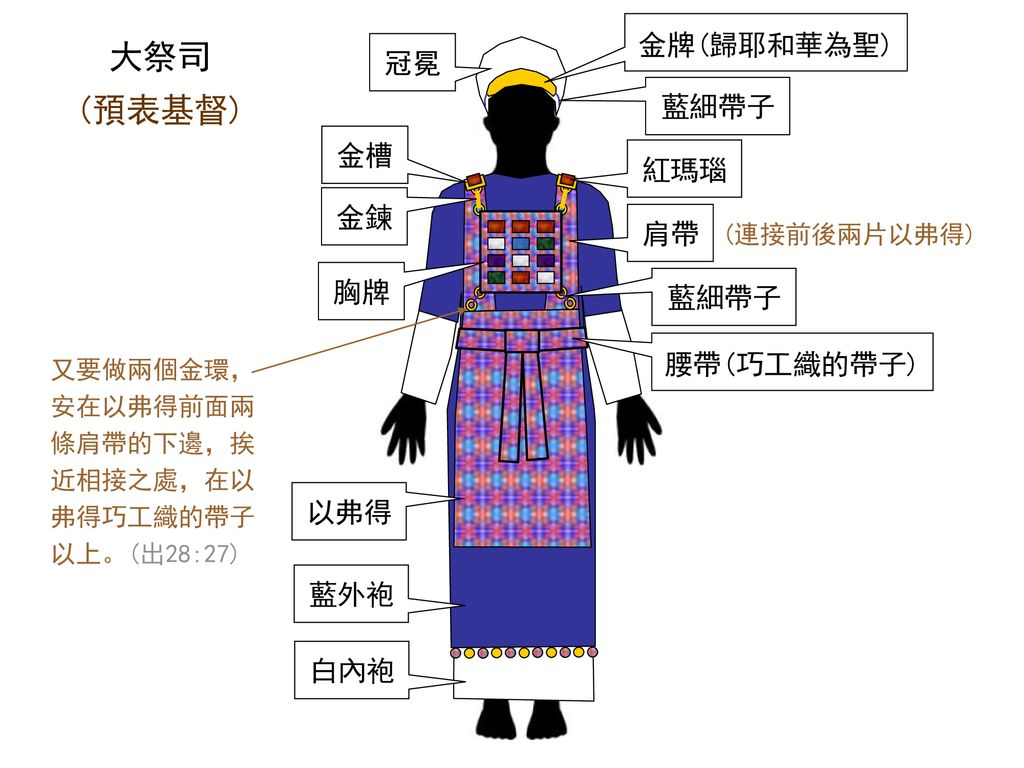
\includegraphics[height=2.5in]{AMoXiFigs/chuaiji/prest2}
       % \caption{}
    \end{subfigure}%
    ~ 
    \begin{subfigure}[b]{0.5\textwidth}
        \centering
        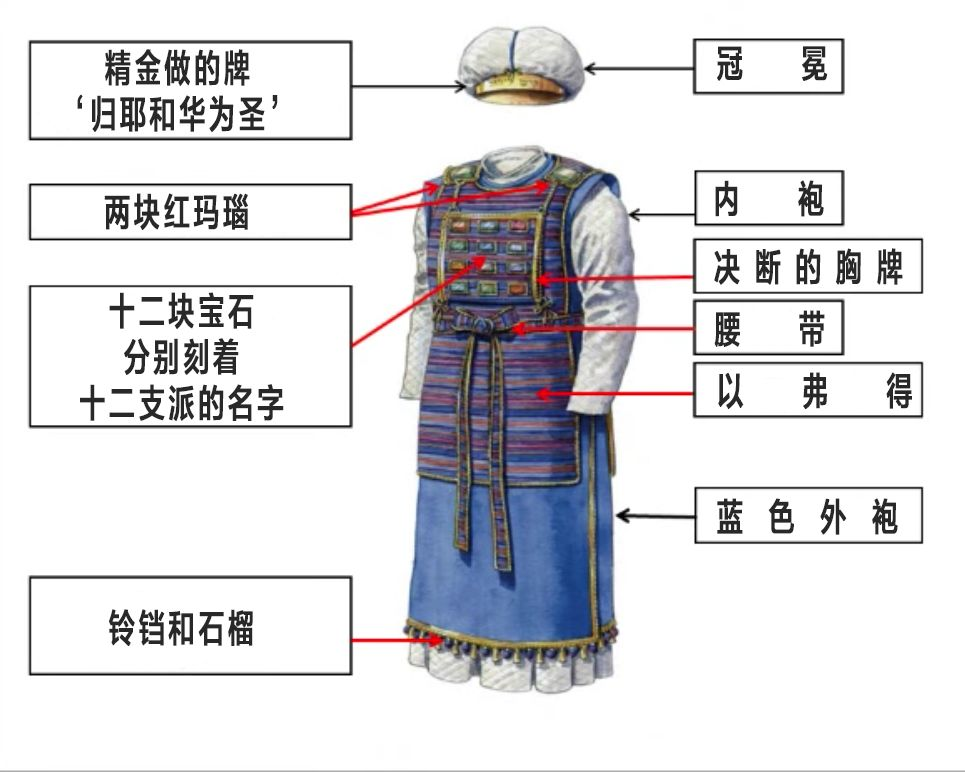
\includegraphics[height=2.5in]{AMoXiFigs/chuaiji/highprest}
      %  \caption{}
    \end{subfigure}
    \caption{祭司服饰图}
\end{figure*}

\subsubsubsection{命亞倫及其后裔為祭司并为其做聖衣 28:1-5}
\begin{itemize} 
\itemsep-.35em
\item 你要從以色列人中，使你的哥哥亞倫和他的兒子拿答、亞比戶、以利亞撒、以他瑪一同就近你，給我供祭司的職分。你要給你哥哥亞倫做聖衣為榮耀，為華美。 
\item 又要吩咐一切心中有智慧的，就是我用智慧的靈所充滿的，給亞倫做衣服，使他分別為聖，可以給我供祭司的職分。所要做的就是胸牌、以弗得、外袍、雜色的內袍、冠冕、腰帶，使你哥哥亞倫和他兒子穿這聖服，可以給我供祭司的職分。要用金線和藍色、紫色、朱紅色線並細麻去做
\end{itemize}
\begin{table}[H]
\centering
\begin{tabular}{|c|c|c| }
\hline
\hline
名稱 &材質　&　章節\\\hline
外袍 & 藍的& 28：31-35 \\\hline
胸牌&（1虎口 X 1虎口）胸牌貼在以弗得巧工織的帶子上&　28：15-30 \\\hline
以弗得&金線和藍色紫色朱紅色線、並撚的細麻&28：6-14　\\\hline
面牌&精金作、在上面刻著、歸耶和華為聖。這牌必在亞倫的額上&28：32-38　\\\hline
內袍&雜色細麻線織&　28：39\\\hline
冠冕&細麻布作&28：39　\\\hline
腰帶&繡花的手工作腰帶&28：39　\\\hline
褲子&細麻布。遮掩下體．褲子當從腰達到大腿&　28：42\\\hline
裹頭巾&亞倫的兒子用&　28：40\\\hline
\end{tabular}
\caption{祭司的服裝}
\end{table}

\subsubsubsection{做以弗得 28:6-14（39:2-7）}
\begin{wrapfigure}{r}{0.3\textwidth}
\vspace{-20pt}
\begin{center}
    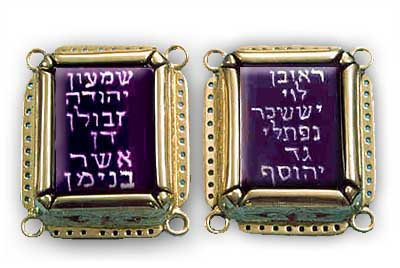
\includegraphics[width=0.3\textwidth]{AMoXiFigs/chuaiji/RedMaNao}
\end{center}
\vspace{-20pt}
  \caption{紅瑪瑙}
 \vspace{-10pt}
\end{wrapfigure}
他們要拿金線和藍色、紫色、朱紅色線並撚的細麻，用巧匠的手工做以弗得。以弗得當有兩條肩帶，接上兩頭，使它相連。其上巧工織的帶子，要和以弗得一樣的做法，用以束上，與以弗得接連一塊，要用金線和藍色、紫色、朱紅色線並撚的細麻做成。
要取兩塊紅瑪瑙，在上面刻以色列兒子的名字，六個名字在這塊寶石上，六個名字在那塊寶石上，都照他們生來的次序。要用刻寶石的手工，彷彿刻圖書，按著以色列兒子的名字刻這兩塊寶石，要鑲在金槽上。要將這兩塊寶石安在以弗得的兩條肩帶上，為以色列人做紀念石。亞倫要在兩肩上擔他們的名字，在耶和華面前作為紀念。
要用金子做二槽，又拿精金，用擰工彷彿擰繩子，做兩條鏈子，把這擰成的鏈子搭在二槽上。


\begin{table}[H]
\centering
\begin{tabular}{|c|c| }
\hline
\hline
材料 & 名稱  \\\hline
以弗得 & 細麻+線（金線，藍色，紫色，朱紅色）   \\\hline
兩條肩帶&細麻+線（金線，藍色，紫色，朱紅色）    \\\hline
兩塊紅瑪瑙&鑲金槽刻以色列兒子的名字 \\\hline
兩條鍊子&　精金、用擰工彷彿擰繩子　\\\hline
\end{tabular}
\caption{以弗得}
\end{table}



\subsubsubsection{做胸牌 28:15-30，39:8-21}
\iffalse
\begin{wraptable}{r}{7.5cm}
\begin{table}[H]
\centering
\begin{tabular}{|c|c|c|c| }
\hline
\hline
第一行 & 紅寶石&紅璧璽&紅玉  \\\hline
第二行&綠寶石&藍寶石&金鋼石  \\\hline
第三行&紫瑪瑙&白瑪瑙&紫晶。 \\\hline
第四行&　水蒼玉&紅瑪瑙&碧玉　\\\hline
\end{tabular}
\caption{胸牌}
\end{table}
\end{wrapfigure}
\fi
你要用巧匠的手工做一個決斷的胸牌。要和以弗得一樣的做法，用金線和藍色、紫色、朱紅色線並撚的細麻做成。這胸牌要四方的，疊為兩層，長一虎口，寬一虎口。要在上面鑲寶石四行：第一行是紅寶石、紅璧璽、紅玉，第二行是綠寶石、藍寶石、金鋼石，第三行是紫瑪瑙、白瑪瑙、紫晶，第四行是水蒼玉、紅瑪瑙、碧玉。這都要鑲在金槽中。
\begin{wrapfigure}{r}{0.3\textwidth}
\vspace{-20pt}
\begin{center}
    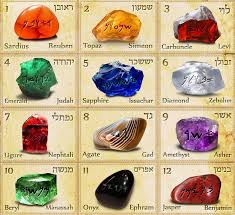
\includegraphics[width=0.3\textwidth]{AMoXiFigs/chuaiji/stones}
\end{center}
\vspace{-10pt}
  \caption{胸牌}
 \vspace{-10pt}
\end{wrapfigure}
這些寶石都要按著以色列十二個兒子的名字，彷彿刻圖書，刻十二個支派的名字。要在胸牌上用精金擰成如繩的鏈子。在胸牌上也要做兩個金環，安在胸牌的兩頭。要把那兩條擰成的金鏈子，穿過胸牌兩頭的環子。又要把鏈子的那兩頭接在兩槽上，安在以弗得前面肩帶上。要做兩個金環，安在胸牌的兩頭，在以弗得裡面的邊上。又要做兩個金環，安在以弗得前面兩條肩帶的下邊，挨近相接之處，在以弗得巧工織的帶子以上。要用藍細帶子把胸牌的環子與以弗得的環子繫住，使胸牌貼在以弗得巧工織的帶子上，不可與以弗得離縫。

亞倫進聖所的時候，要將決斷胸牌，就是刻著以色列兒子名字的，戴在胸前，在耶和華面前常做紀念。又要將烏陵和土明放在決斷的胸牌裡。亞倫進到耶和華面前的時候，要戴在胸前，在耶和華面前常將以色列人的決斷牌戴在胸前


\begin{table}[H]
    \begin{minipage}{.5\linewidth}
      \centering
       \begin{tabular}{|c|c|c|c| }
\hline
\hline
第一行 & 紅寶石&紅璧璽&紅玉  \\\hline
第二行&綠寶石&藍寶石&金鋼石  \\\hline
第三行&紫瑪瑙&白瑪瑙&紫晶。 \\\hline
第四行&　水蒼玉&紅瑪瑙&碧玉　\\\hline
\end{tabular}
   \caption{胸牌}
    \end{minipage}%
    \begin{minipage}{.5\linewidth}
      \centering    
     \begin{tabular}{|c|c| }
\hline
\hline
外袍 & 藍的  \\\hline
領口&口的周圍織出領邊  \\\hline
石榴&藍色+紫色+朱紅色線 \\\hline
金鈴鐺&金　\\\hline
\end{tabular}
%  \caption{以弗得外袍}
    \end{minipage} 
\end{table}


\subsubsubsection{製造以弗得外袍的規定 28:31-35（39:22-26）}
\begin{itemize} 
\itemsep-.35em
\item 你要做以弗得的外袍顏色全是藍的。袍上要為頭留一領口，口的周圍織出領邊來彷彿鎧甲的領口免得破裂
\item 袍子周圍底邊上要用藍色、紫色、朱紅色線做石榴，在袍子周圍的石榴中間要有金鈴鐺。一個金鈴鐺一個石榴，一個金鈴鐺一個石榴，在袍子周圍的底邊上。
\item 亞倫供職的時候要穿這袍子。他進聖所到耶和華面前以及出來的時候，袍上的響聲必被聽見使他不至死亡
\end{itemize}


\subsubsubsection{製造面牌的規定 28:36-38}
\begin{itemize} 
\itemsep-.35em
\item 你要用精金做一面牌，在上面按刻圖書之法刻著：歸耶和華為聖。要用一條藍細帶子將牌繫在冠冕的前面。
\item 這牌必在亞倫的額上，亞倫要擔當干犯聖物條例的罪孽，這聖物是以色列人在一切的聖禮物上所分別為聖的。這牌要常在他的額上，使他們可以在耶和華面前蒙悅納。
\end{itemize}

\subsubsubsection{製造內袍冠冕腰帶裹頭巾褲子 28:39-43（39:27-29）}
\begin{itemize} 
\itemsep-.35em
\item 要用雜色細麻線織內袍，用細麻布做冠冕，又用繡花的手工做腰帶。你要為亞倫的兒子做內袍、腰帶、裹頭巾，為榮耀，為華美。要把這些給你的哥哥亞倫和他的兒子穿戴，又要膏他們，將他們分別為聖，好給我供祭司的職分。 
\item 要給他們做細麻布褲子，遮掩下體，褲子當從腰達到大腿。亞倫和他兒子進入會幕，或就近壇，在聖所供職的時候必穿上，免得擔罪而死。這要為亞倫和他的後裔做永遠的定例
\end{itemize}

\subsubsection{祭司分别为圣的禮仪 29}
\subsubsubsection{祭司承接聖職的穿戴 29:1-9 }
\begin{itemize} 
\itemsep-.35em
\item 你使亞倫和他兒子成聖，給我供祭司的職分，要如此行。
\begin{itemize} 
\itemsep-.35em
\item 献祭：取一隻\underline{公牛犢}，兩隻無殘疾的\underline{公綿羊}，\underline{無酵餅}和\underline{調油的無酵餅}，與\underline{抹油的無酵薄餅}，這都要用細麥麵做成。這餅要裝在一個筐子裡，連筐子帶來，又把公牛和兩隻公綿羊牽來。
\item 要使亞倫和他兒子到會幕門口來用水洗身。 
\begin{itemize} 
\itemsep-.35em
\item 要給亞倫穿上內袍和以弗得的外袍並以弗得，又戴上胸牌，束上以弗得巧工織的帶子。 6 把冠冕戴在他頭上，將聖冠加在冠冕上，就把膏油倒在他頭上膏他。 
\item 要叫他的兒子來，給他們穿上內袍。 
\item 給亞倫和他兒子束上腰帶，包上裹頭巾，
\end{itemize} 
\end{itemize}
\item 他們就憑永遠的定例得了祭司的職任。又要將亞倫和他兒子分別為聖
\end{itemize}


\subsubsubsection{承接聖職的贖罪祭-公牛 29:10-14 （利8:14-17）}
\begin{itemize} 
\itemsep-.35em
\item 你要把公牛牽到會幕前，亞倫和他兒子要按手在公牛的頭上。 
\item 你要在耶和華面前，在會幕門口，宰這公牛。要取些公牛的血，用指頭抹在壇的四角上，把血都倒在壇腳那裡。要把一切蓋臟的脂油與肝上的網子，並兩個腰子和腰子上的脂油，都燒在壇上。只是公牛的皮、肉、糞都要用火燒在營外。這牛是\underline{贖罪祭}
\end{itemize}

\subsubsubsection{承接聖職的燔祭-一隻公綿羊 29:15-18 （利8:18-21）}
\begin{itemize} 
\itemsep-.35em
\item 你要牽一隻公綿羊來，亞倫和他兒子要按手在這羊的頭上。 
\item 要宰這羊，把血灑在壇的周圍。要把羊切成塊子，洗淨五臟和腿，連塊子帶頭，都放在一處。要把全羊燒在壇上，是給耶和華獻的\underline{燔祭}，是獻給耶和華為馨香的\underline{火祭}
\end{itemize}

\subsubsubsection{承接聖職的公綿羊-搖祭及舉祭 29:19-25 （利8:22-29）}
\begin{itemize} 
\itemsep-.35em
\item 你要將那一隻公綿羊牽來，亞倫和他兒子要按手在羊的頭上。你要宰這羊，取點血抹在亞倫的右耳垂上和他兒子的右耳垂上，又抹在他們右手的大拇指上和右腳的大拇指上，並要把血灑在壇的四圍。你要取點膏油和壇上的血，彈在亞倫和他的衣服上，並他兒子和他兒子的衣服上，\underline{他們和他們的衣服就一同成聖} 。 
\item 搖祭放在燔祭上燒=馨香的火祭
\begin{itemize} 
\itemsep-.35em
\item 你要取這羊的脂油和肥尾巴，並蓋臟的脂油與肝上的網子，兩個腰子和腰子上的脂油並右腿，這是承接聖職所獻的羊。再從耶和華面前裝無酵餅的筐子中取一個餅，一個調油的餅和一個薄餅，都放在亞倫的手上和他兒子的手上，作為\underline{搖祭}，在耶和華面前搖一搖。
\item 要從他們手中接過來，\underline{燒在}耶和華面前壇上的\underline{燔祭}上，是獻給耶和華為馨香的\underline{火祭}。
\end{itemize}
\end{itemize}

\subsubsubsection{承接聖職的其他禮儀 29:29-37 （利8:30-35）}
\begin{itemize} 
\itemsep-.35em
\item 亞倫的聖衣要留給他的子孫，可以穿著受膏，又穿著承接聖職。他的子孫接續他當祭司的，每逢進會幕在聖所供職的時候，要穿七天。
\item 你要將承接聖職所獻公羊的肉煮在聖處。亞倫和他兒子要在會幕門口吃這羊的肉和筐內的餅。他們吃那些贖罪之物，好承接聖職，使他們成聖；只是外人不可吃，因為這是聖物。那承接聖職所獻的肉或餅，若有一點留到早晨，就要用火燒了，不可吃這物，因為是聖物。
\item 你要這樣照我一切所吩咐的，向亞倫和他兒子行承接聖職的禮七天。每天要獻公牛一隻為贖罪祭。你潔淨壇的時候，壇就潔淨了，且要用膏抹壇，使壇成聖。要潔淨壇七天，使壇成聖，壇就成為至聖。凡挨著壇的都成為聖
\end{itemize}


\subsubsubsection{祭司每天當獻的祭物 29:38-46 }
\begin{itemize} 
\itemsep-.35em
\item 你每天所要獻在壇上的就是兩隻一歲的羊羔，早晨要獻這一隻，黃昏的時候要獻那一隻。和這一隻羊羔同獻的，要用細麵伊法十分之一與搗成的油一欣四分之一調和，又用酒一欣四分之一作為奠祭。那一隻羊羔要在黃昏的時候獻上，照著早晨的素祭和奠祭的禮辦理，作為獻給耶和華馨香的火祭。
\item 這要在耶和華面前，會幕門口，做你們世世代代常獻的燔祭。我要在那裡與你們相會，和你們說話。我要在那裡與以色列人相會，會幕就要因我的榮耀成為聖。我要使會幕和壇成聖，也要使亞倫和他的兒子成聖，給我供祭司的職分。
\item 我要住在以色列人中間，做他們的神。他們必知道我是耶和華他們的神，是將他們從埃及地領出來的，為要住在他們中間。我是耶和華他們的神
\end{itemize}
\begin{table}[H]
\centering
\begin{tabular}{|c|c|c|c|c|c|c| }
\hline
\hline
天&贖罪祭 & 燔祭&承接聖職獻的祭 &素祭 &搖祭 & 舉祭\\\hline
1&公牛& 公綿羊（1) &公綿羊（1) & 無酵餅 &無酵餅（1) & 承接聖職公綿羊的腿\\\hline
 &&   & & 調油的無酵餅  & 調油的餅 （1) & \\\hline
 & &   & & 抹油的無酵薄餅 & 薄餅（1) &\\\hline
& &   & &   & 承接聖職公綿羊的胸 & \\\hline
2& 公牛&   & &   &   & \\\hline
3&公牛 &   & &   &   & \\\hline
4&公牛 &   & &   &   & \\\hline
5&公牛 &   & &   &   & \\\hline
6&公牛 &   & &   &   & \\\hline
7&公牛 &   & &   &  & \\\hline
\end{tabular}
\caption{承接聖職獻的7天祭}
\end{table}


\subsubsection{其它会幕物品制作服事條例 30-31}
\subsubsubsection{造香壇的條例 30:1-6，37:25-28}
\begin{itemize} 
\itemsep-.35em
\item 你要用皂莢木做一座燒香的壇。這壇要四方的，長一肘，寬一肘，高二肘。壇的四角要與壇接連一塊。要用精金把壇的上面與壇的四圍並壇的四角包裹
\item 又要在壇的四圍鑲上金牙邊。要做兩個金環安在牙子邊以下，在壇的兩旁兩根橫撐上，作為穿槓的用處，以便抬壇。要用皂莢木做槓，用金包裹。
\item 要把壇放在法櫃前的幔子外，對著法櫃上的施恩座，就是我要與你相會的地方。 
\end{itemize}

\subsubsubsection{亞倫在壇上的服事條例 30:7-10}
\vspace*{-5mm}
 \begin{itemize} 
\itemsep-.35em
\item 亞倫在壇上要燒馨香料做的香，每早晨他收拾燈的時候，要燒這香。黃昏點燈的時候，他要在耶和華面前燒這香，作為世世代代常燒的香。在這壇上不可奉上異樣的香，不可獻燔祭、素祭，也不可澆上奠祭。
\item 亞倫一年一次要在壇的角上行贖罪之禮。他一年一次要用贖罪祭牲的血在壇上行贖罪之禮，作為世世代代的定例。這壇在耶和華面前為至聖。
\end{itemize}

\subsubsubsection{每人當獻贖命之價 30:11-16 （37:25-28）}
\begin{itemize} 
\itemsep-.35em
\item 耶和華曉諭摩西說：「你要按以色列人被數的計算總數，你數的時候，他們各人要為自己的生命把贖價奉給耶和華，免得數的時候在他們中間有災殃。凡過去歸那些被數之人的，每人要按聖所的平，拿銀子半舍客勒，這半舍客勒是奉給耶和華的禮物，一舍客勒是二十季拉。凡過去歸那些被數的人，從二十歲以外的，要將這禮物奉給耶和華。
\item 他們為贖生命將禮物奉給耶和華，富足的不可多出，貧窮的也不可少出，各人要出半舍客勒。你要從以色列人收這贖罪銀，作為會幕的使用，可以在耶和華面前為以色列人做紀念，贖生命。
\end{itemize}

\subsubsubsection{造銅盆的規定 30:17-21 （38:8）}
\begin{itemize} 
\itemsep-.35em
\item 耶和華曉諭摩西說：你要用銅做洗濯盆和盆座，以便洗濯。要將盆放在會幕和壇的中間，在盆裡盛水。
\item 亞倫和他的兒子要在這盆裡洗手洗腳。他們進會幕，或是就近壇前供職給耶和華\underline{獻火祭}的時候，\underline{必用水洗濯}，免得死亡。他們洗手洗腳，就免得死亡。這要做亞倫和他後裔世世代代永遠的定例。
\end{itemize}


\subsubsubsection{製作聖膏油的規定 30:22-33}
\begin{wraptable}{r}{4.2cm}
\vspace*{-\baselineskip}
\begin{tabular}{ll }
\hline
\hline
聖膏油製作& 份量 \\\hline
沒藥 & 500舍客勒 \\\hline
香肉桂&250舍客勒  \\\hline
菖蒲&250舍客勒   \\\hline
桂皮&500舍客勒   \\\hline
橄欖油&1欣 \\\hline
\end{tabular}
\caption{聖膏油的規定}
\end{wraptable}
耶和華曉諭摩西說： 「你要取上品的香料，就是流質的沒藥五百舍客勒，香肉桂一半，就是二百五十舍客勒，菖蒲二百五十舍客勒，桂皮五百舍客勒，都按著聖所的平，又取橄欖油一欣，按做香之法調和做成聖膏油。\\
要用這膏油抹會幕和法櫃，桌子與桌子的一切器具，燈臺和燈臺的器具並香壇，燔祭壇和壇的一切器具，洗濯盆和盆座。要使這些物成為聖，好成為至聖，凡挨著的都成為聖。要膏亞倫和他的兒子，使他們成為聖，可以給我供祭司的職分。\\
你要對以色列人說：『這油，我要世世代代以為聖膏油。不可倒在別人的身上，也不可按這調和之法做與此相似的。這膏油是聖的，你們也要以為聖。凡調和與此相似的，或將這膏膏在別人身上的，這人要從民中剪除。』



\iffalse
\begin{table}[H]
    \begin{subtable}{.5\linewidth}
 \centering  
\begin{tabular}{ll }
\hline
\hline
聖膏油製作& 份量 \\\hline
沒藥 & 500舍客勒 \\\hline
香肉桂&250舍客勒  \\\hline
菖蒲&250舍客勒   \\\hline
桂皮&500舍客勒   \\\hline
橄欖油&1欣 \\\hline
\end{tabular}
\caption{聖膏油和聖香的規定}
    \end{subtable}%
    \begin{subtable}{.5\linewidth}
      \centering    
    \begin{tabular}{ll}
\hline
\hline
聖香製作 &份量\\\hline
 拿他弗 & 1份  \\\hline
  施喜列 &1份 \\\hline
 喜利比拿 &1份  \\\hline
 淨乳香 &1份 \\\hline
 鹽 &\\\hline
\end{tabular}
   \caption{聖香製作}
    \end{subtable} 
\end{table}
\fi

\subsubsubsection{製作聖香的規定 30:34-38}
\begin{wraptable}{r}{5cm}
%\vspace*{-\baselineskip}
\vspace*{-10mm}
   \begin{tabular}{ll}
\hline
\hline
聖香製作 &份量\\\hline
 拿他弗 & 1份  \\\hline
  施喜列 &1份 \\\hline
 喜利比拿 &1份  \\\hline
 淨乳香 &1份 \\\hline
 鹽 &\\\hline
\end{tabular}
\caption{聖香製作}
\end{wraptable}
耶和華吩咐摩西說：「你要取馨香的香料，就是拿他弗、施喜列、喜利比拿，這馨香的香料和淨乳香各樣要一般大的分量。你要用這些加上鹽，按做香之法做成清淨聖潔的香。這香要取點搗得極細，放在會幕內法櫃前，我要在那裡與你相會。\\
你們要以這香為至聖。你們不可按這調和之法為自己做香，要以這香為聖，歸耶和華。凡做香和這香一樣，為要聞香味的，這人要從民中剪除。


\subsubsubsection{神提名比撒列,亞何利亞伯造會幕 31:1-11 （35:30-35）}
%\begin{wraptable}{r}{7.5cm}
\begin{table}[H]
\vspace*{-\baselineskip}
%\vspace*{1.0cm}
\center
\begin{tabular}{ c c c c }
\toprule
支派 & 爺爺名字 & 父親名字& 技工 \\\hline
猶大&戶珥  &  烏利 & 比撒列\\\hline
但&  & 亞希撒抹& 亞何利亞伯 \\\hline
\end{tabular}
\caption{技工比撒列,亞何利亞伯}
\end{table} 
%\end{wraptable}
%\vspace*{-\baselineskip}
耶和華曉諭摩西說：「看哪，猶大支派中，戶珥的孫子、烏利的兒子比撒列，我已經提他的名召他。我也以我的靈充滿了他，使他有智慧，有聰明，有知識，能做各樣的工， 能想出巧工，用金、銀、銅製造各物，又能刻寶石，可以鑲嵌，能雕刻木頭，能做各樣的工。\\
我分派但支派中亞希撒抹的兒子亞何利亞伯與他同工。\underline{\textcolor{blue}{凡}心裡有智慧的，我\textcolor{blue}{更}使他們有智慧，\textcolor{blue}{能}做我一切所吩咐的}，就是會幕和法櫃，並其上的施恩座，與會幕中一切的器具，桌子和桌子的器具，精金的燈臺和燈臺的一切器具並香壇， 燔祭壇和壇的一切器具，並洗濯盆與盆座，精工做的禮服，和祭司亞倫並他兒子用以供祭司職分的聖衣，膏油和為聖所用馨香的香料。他們都要照我一切所吩咐的去做。」
%\end{itemize}


\subsubsubsection{當守安息日為證 31:12-18}
\begin{itemize}
\itemsep-.35em
\item 耶和華曉諭摩西說：「你要吩咐以色列人說：『你們務要守我的安息日，因為這是你我之間世世代代的證據，使你們知道我\underline{耶和華是叫你們成為聖的。所以你們要守安息日，以為聖日}。凡干犯這日的，必要把他治死；凡在這日做工的，必從民中剪除。六日要做工，但第七日是安息聖日，是向耶和華守為聖的。凡在安息日做工的，必要把他治死。故此，以色列人要世世代代守安息日為永遠的約。這是我和以色列人永遠的證據，因為六日之內\underline{耶和華造天地，第七日便安息舒暢}。』」
\item 耶和華在西奈山和摩西說完了話，就把兩塊法版交給他，是神用指頭寫的石版。
\end{itemize}

\subsection{摩西四次上山為百姓拜金牛犢代求 32-34}
\subsubsection{亞倫造犢 32:1-6}
\begin{itemize}
\itemsep-.35em
\item 百姓見摩西遲延不下山，就大家聚集到亞倫那裡，對他說：「起來，為我們做神像，可以在我們前面引路，因為領我們出埃及地的那個摩西，我們不知道他遭了什麼事。」 
\item 亞倫對他們說：「你們去摘下你們妻子、兒女耳上的金環，拿來給我。」
\begin{itemize}
\itemsep-.35em
\item 百姓就都摘下他們耳上的金環，拿來給亞倫。 
 \item 亞倫從他們手裡接過來，鑄了一隻牛犢，用雕刻的器具做成。他們就說：「以色列啊，這是領你出埃及地的神！」亞倫看見，就在牛犢面前築壇，且宣告說：「明日要向耶和華守節。」 
\item 次日清早，百姓起來獻燔祭和平安祭，就坐下吃喝，起來玩耍。
\end{itemize}
\end{itemize}

\subsubsection{摩西第一次為百姓代求 32:7-14}
\begin{table}[H]
\begin{threeparttable}
\begin{tabular}{@{}p{0.4\textwidth}*{4}{L{\dimexpr0.7\linewidth-10\tabcolsep\relax}}@{}}
\toprule
神 &  摩西 \\\hline
耶和華吩咐摩西說：「下去吧，因為你的百姓，就是你從埃及地領出來的，已經敗壞了。他們快快偏離了我所吩咐的道，為自己鑄了一隻牛犢，向它下拜獻祭，說：『以色列啊，這就是領你出埃及地的神！』」&\tabularnewline\hline
耶和華對摩西說：「我看這百姓真是硬著頸項的百姓。你且由著我，我要向他們發烈怒，將他們滅絕，使你的後裔成為大國。」&摩西便懇求耶和華他的神說：「耶和華啊，你為什麼向你的百姓發烈怒呢？這百姓是你用大力和大能的手從埃及地領出來的。為什麼使埃及人議論說『他領他們出去，是要降禍於他們，把他們殺在山中，將他們從地上除滅』？求你轉意，不發你的烈怒；後悔，不降禍與你的百姓。求你記念你的僕人亞伯拉罕、以撒、以色列，你曾指著自己起誓說：『我必使你們的後裔像天上的星那樣多，並且我所應許的這全地，必給你們的後裔，他們要永遠承受為業。』」\tabularnewline\hline
於是耶和華後悔，不把所說的禍降於他的百姓&\tabularnewline
\bottomrule
\end{tabular}
%\caption{摩西第一次為百姓代求}
\end{threeparttable}
\end{table} 


\subsubsection{摩西怒摔法版 32:15-29}
\begin{itemize}
\itemsep-.35em
\item 摩西轉身下山手裡拿著兩塊法版。這版是兩面寫的這面那面都有字，是神的工作，字是神寫的刻在版上。約書亞一聽見百姓呼喊的聲音，就對摩西說：「在營裡有爭戰的聲音。」摩西說：「這不是人打勝仗的聲音，也不是人打敗仗的聲音，我所聽見的乃是人歌唱的聲音。」
\item 摩西挨近營前，就看見牛犢，又看見人跳舞，便發烈怒，把兩塊版扔在山下摔碎了，又將他們所鑄的牛犢用火焚燒，磨得粉碎，撒在水面上，叫以色列人喝。摩西對亞倫說：「這百姓向你做了什麼？你竟使他們陷在大罪裡！」亞倫說：「求我主不要發烈怒。這百姓專於作惡，是你知道的。他們對我說：『你為我們做神像，可以在我們前面引路，因為領我們出埃及地的那個摩西，我們不知道他遭了什麼事。』我對他們說：『凡有金環的，可以摘下來。』他們就給了我，我把金環扔在火中，這牛犢便出來了。」
\item 三千百姓被利未的子孫殺死
\begin{table}[H]
\begin{threeparttable}
\begin{tabular}{@{}p{0.6\textwidth}*{4}{L{\dimexpr0.5\linewidth-10\tabcolsep\relax}}@{}}
\toprule
摩西 & 利未的子孫 \\\hline
摩西見百姓放肆（亞倫縱容他們，使他們在仇敵中間被譏刺），就站在營門中，說：「凡屬耶和華的，都要到我這裡來！」&於是利未的子孫都到他那裡聚集。\tabularnewline\hline
他對他們說：「耶和華以色列的神這樣說：『你們各人把刀跨在腰間，在營中往來，從這門到那門，各人殺他的弟兄與同伴並鄰舍。』」 &利未的子孫照摩西的話行了。那一天百姓中被殺的約有三千\tabularnewline\hline
摩西說：「今天你們要自潔，歸耶和華為聖，各人攻擊他的兒子和弟兄，使耶和華賜福於你們。」 &\tabularnewline
\bottomrule
\end{tabular}
\caption{三千百姓被利未的子孫殺死}
\end{threeparttable}
\end{table} 
\end{itemize}

\subsubsection{摩西第二次為百姓代求 32:30-33:3}
\begin{table}[H]
\begin{threeparttable}
\begin{tabular}{@{}p{0.4\textwidth}*{4}{L{\dimexpr0.6\linewidth-10\tabcolsep\relax}}@{}}
\toprule
摩西 &  神 \\\hline
到了第二天，摩西對百姓說:你們犯了大罪，我如今要上耶和華那裡去，或者可以為你們贖罪&\tabularnewline\hline
摩西回到耶和華那裡，說：「唉！這百姓犯了大罪，為自己做了金像。倘或你肯赦免他們的罪——不然，求你從你所寫的冊上塗抹我的名。」&耶和華對摩西說：「誰得罪我，我就從我的冊上塗抹誰的名。現在你去領這百姓，往我所告訴你的地方去，我的使者必在你前面引路，只是到我追討的日子，我必追討他們的罪。」\tabularnewline\hline
&耶和華殺百姓的緣故是因他們同亞倫做了牛犢。\tabularnewline\hline
&耶和華吩咐摩西說：「我曾起誓應許亞伯拉罕、以撒、雅各說：『要將迦南地賜給你的後裔。』現在你和你從埃及地所領出來的百姓，要從這裡往那地去。我要差遣使者在你前面，攆出迦南人、亞摩利人、赫人、比利洗人、希未人、耶布斯人領你到那流奶與蜜之地。我自己不同你們上去，因為你們是硬著頸項的百姓，恐怕我在路上把你們滅絕。」\tabularnewline
\bottomrule
\end{tabular}
%\caption{摩西第二次為百姓代求}
\end{threeparttable}
\end{table} 

\subsubsection{百姓除淨身上佩戴裝飾 33:4-6}
\begin{itemize}
\itemsep-.35em
\item 百姓聽見這凶信就悲哀，也沒有人佩戴裝飾。 
\item 耶和華對摩西說：「你告訴以色列人說：『耶和華說：你們是硬著頸項的百姓，我若一霎時臨到你們中間，必滅絕你們。現在你們要把身上的裝飾摘下來，使我可以知道怎樣待你們。』」 
\item 以色列人從住何烈山以後，就把身上的裝飾摘得乾淨
\end{itemize}

\subsubsection{摩西與神會面的會幕——支搭在的營外帳篷 33:7-11}
\begin{itemize}
\itemsep-.35em
\item 摩西素常將帳篷支搭在營外，離營卻遠，他稱這帳篷為會幕。凡求問耶和華的，就到營外的會幕那裡去。 
\begin{itemize}
\itemsep-.35em
\item 當摩西出營到會幕去的時候，百姓就都起來，各人站在自己帳篷的門口，望著摩西，直等到他進了會幕。
 \item 摩西進會幕的時候，雲柱降下來，立在會幕的門前，耶和華便與摩西說話。
\item 眾百姓看見雲柱立在會幕門前，就都起來，各人在自己帳篷的門口下拜。
\item 耶和華與摩西面對面說話，好像人與朋友說話一般。
\end{itemize}
\item 摩西轉到營裡去，唯有他的幫手，一個少年人嫩的兒子約書亞，不離開會幕。
\end{itemize}


\subsubsection{摩西求耶和華同往,并蒙恩见神的荣耀 33:12-23}
\begin{table}[H]
\begin{threeparttable}
\begin{tabular}{@{}p{0.4\textwidth}*{4}{L{\dimexpr0.7\linewidth-10\tabcolsep\relax}}@{}}
\toprule
摩西的祈祷 &  神的应许 \\\hline
摩西對耶和華說：「你吩咐我說：『將這百姓領上去』，卻沒有叫我知道你要打發誰與我同去，只說：『我按你的名認識你，你在我眼前也蒙了恩。』 我如今若在你眼前蒙恩，求你將你的道指示我，使我可以認識你，好在你眼前蒙恩。求你想到這民是你的民。」&耶和華說：「我必親自和你同去，使你得安息。」\tabularnewline\hline
摩西說：「你若不親自和我同去，就不要把我們從這裡領上去。人在何事上得以知道我和你的百姓在你眼前蒙恩呢？豈不是因你與我們同去，使我和你的百姓與地上的萬民有分別嗎？」&耶和華對摩西說：「你這所求的我也要行，因為你在我眼前蒙了恩，並且我按你的名認識你。」 \tabularnewline\hline
摩西說：「求你顯出你的榮耀給我看。」&耶和華說：「我要顯我一切的恩慈，在你面前經過，宣告我的名。我要恩待誰就恩待誰，要憐憫誰就憐憫誰。」 \tabularnewline\hline
&又說：「你不能看見我的面，因為人見我的面不能存活。」 \tabularnewline\hline
&耶和華說：「看哪，在我這裡有地方，你要站在磐石上。我的榮耀經過的時候，我必將你放在磐石穴中，用我的手遮掩你，等我過去。然後我要將我的手收回，你就得見我的背，卻不得見我的面。」 \tabularnewline
\bottomrule
\end{tabular}
\caption{摩西求耶和華同往,并蒙恩见神的荣耀}
\end{threeparttable}
\end{table} 

\subsubsection{摩西復上西奈山，新鑿兩塊石版 34:1-4 （申10:1-5）}
耶和華吩咐摩西說：「你要鑿出兩塊石版，和先前你摔碎的那版一樣，其上的字我要寫在這版上。明日早晨，你要預備好了，上西奈山，在山頂上站在我面前。誰也不可和你一同上去，遍山都不可有人，在山根也不可叫羊群牛群吃草。」 \\
摩西就鑿出兩塊石版，和先前的一樣。清晨起來，照耶和華所吩咐的上西奈山去，手裡拿著兩塊石版。

\subsubsection{耶和華宣告自己的名 34:5-9}
耶和華在雲中降臨，和摩西一同站在那裡，宣告耶和華的名。耶和華在他面前宣告說：「耶和華，耶和華，是有憐憫有恩典的神，不輕易發怒，並有豐盛的慈愛和誠實。為千萬人存留慈愛，赦免罪孽、過犯和罪惡；萬不以有罪的為無罪，必追討他的罪，自父及子，直到三四代。」 \\
摩西急忙伏地下拜，說：「主啊，我若在你眼前蒙恩，求你在我們中間同行，因為這是硬著頸項的百姓。又求你赦免我們的罪孽和罪惡，以我們為你的產業。」

\subsubsection{耶和華和立約，并禁止百姓拜別神 34:10-17}
耶和華說：「我要立約，要在百姓面前行奇妙的事，是在遍地萬國中所未曾行的。在你四圍的外邦人就要看見耶和華的作為，因我向你所行的是可畏懼的事。我今天所吩咐你的，你要謹守。我要從你面前攆出亞摩利人、迦南人、赫人、比利洗人、希未人、耶布斯人。\\
你要謹慎，\underline{不可}與你所去那地的居民立約，恐怕成為你們中間的網羅；卻要拆毀他們的祭壇，打碎他們的柱像，砍下他們的木偶。\underline{不可}敬拜別神，因為耶和華是忌邪的神，名為忌邪者。只怕你與那地的居民立約，百姓隨從他們的神，就行邪淫，祭祀他們的神，有人叫你，你便吃他的祭物；又為你的兒子娶他們的女兒為妻，他們的女兒隨從她們的神，就行邪淫，使你的兒子也隨從她們的神行邪淫。\underline{不可}為自己鑄造神像。

\subsubsection{守除酵節,安息日,七七節,收藏節 34:16-26}
你要守\underline{除酵節}，照我所吩咐你的，在亞筆月內所定的日期吃無酵餅七天，因為你是這亞筆月內出了埃及。凡\underline{頭生}的都是我的，一切牲畜頭生的，無論是牛是羊，公的都是我的。頭生的驢要用羊羔代贖，若不代贖就要打折牠的頸項。凡頭生的兒子都要贖出來。誰也不可空手朝見我。\\
你六日要做工，第七日要安息；雖在耕種收割的時候，也要安息。在收割初熟麥子的時候要守\underline{七七節}，又在年底要守\underline{收藏節}。你們一切男丁要一年三次朝見主耶和華以色列的神。我要從你面前趕出外邦人，擴張你的境界。你一年三次上去朝見耶和華你神的時候，必沒有人貪慕你的地土。\\
你不可將我祭物的血和有酵的餅一同獻上，逾越節的祭物也不可留到早晨。地裡首先初熟之物要送到耶和華你神的殿。不可用山羊羔母的奶煮山羊羔。\\

\subsubsection{摩西四十晝夜不吃飯不喝水 34:27-28}
耶和華吩咐摩西說：「你要將這些話寫上，因為我是按這話與你和以色列人立約。」摩西在耶和華那裡四十晝夜，也不吃飯，也不喝水。耶和華將這約的話，就是十條誡，寫在兩塊版上。

\subsubsection{摩西面容發光 34:16-26}
摩西手裡拿著兩塊法版下西奈山的時候，不知道自己的面皮因耶和華和他說話就發了光。亞倫和以色列眾人看見摩西的面皮發光，就怕挨近他。摩西叫他們來，於是亞倫和會眾的官長都到他那裡去，摩西就與他們說話。隨後以色列眾人都近前來，他就把耶和華在西奈山與他所說的一切話都吩咐他們。摩西與他們說完了話，就用帕子蒙上臉。但摩西進到耶和華面前與他說話就揭去帕子，及至出來的時候，便將耶和華所吩咐的告訴以色列人。以色列人看見摩西的面皮發光。摩西又用帕子蒙上臉，等到他進去與耶和華說話，就揭去帕子

\subsection{摩西传神的話，造會幕和祭司服 35-40}
\subsubsection{守安息日之例 35:1-2}
摩西招聚以色列全會眾，對他們說：「這是耶和華所吩咐的話，叫你們照著行。六日要做工，第七日乃為聖日，\underline{當向耶和華守為安息聖日}。凡這日之內做工的，必把他治死。當安息日，不可在你們一切的住處生火。」

\subsubsection{呼召會眾獻禮物 35:4-9 （25:1-7）}
\begin{wraptable}{r}{10.5cm}
%\begin{table}[!hbp]
%\centering
%\vspace*{-\baselineskip}
\vspace*{-1cm}
\begin{tabular}{|c|c| }
\hline
\hline
材料 & 名稱  \\\hline
金屬 & 金、銀、銅    \\\hline
線類&藍色、紫色、朱紅色線、細麻、山羊毛  \\\hline
皮類&染紅的公羊皮、海狗皮 \\\hline
木類&　皂莢木 　\\\hline
油、香料&點燈的油並做膏油和香的香料　\\\hline
寶石&紅瑪瑙與別樣的寶石，可以鑲嵌在以弗得和胸牌上 \\\hline
\end{tabular}
\caption{呼召會眾奉獻的物}
%\end{table}
\end{wraptable} 
摩西對以色列全會眾說：「耶和華所吩咐的是這樣：你們中間要拿禮物獻給耶和華，凡樂意獻的，可以拿耶和華的禮物來，就是金，銀，銅，藍色、紫色、朱紅色線，細麻，山羊毛，染紅的公羊皮，海狗皮，皂莢木，點燈的油，並做膏油和香的香料，紅瑪瑙與別樣的寶石，可以鑲嵌在以弗得和胸牌上。

\subsubsection{呼召有智慧的来做神的工及工作内容 35:10-19 (39:32-41)}
你們中間凡心裡有智慧的，都要來做耶和華一切所吩咐的，就是帳幕和帳幕的罩篷，並帳幕的蓋、鉤子、板、閂、柱子、帶卯的座，櫃和櫃的槓，施恩座和遮掩櫃的幔子，桌子和桌子的槓與桌子的一切器具，並陳設餅，燈臺和燈臺的器具，燈盞並點燈的油，香壇和壇的槓，膏油和馨香的香料，並帳幕門口的簾子，燔祭壇和壇的銅網，壇的槓並壇的一切器具，洗濯盆和盆座，院子的帷子和帷子的柱子，帶卯的座和院子的門簾，帳幕的橛子並院子的橛子和這兩處的繩子，精工做的禮服和祭司亞倫並他兒子在聖所用以供祭司職分的聖衣。

\subsubsection{會眾回应獻禮物的呼召 35:20-29}
以色列全會眾從摩西面前退去。凡心裡受感和甘心樂意的，都拿耶和華的禮物來，用以做會幕和其中一切的使用，又用以做聖衣。凡心裡樂意獻禮物的，連男帶女，各將金器，就是胸前針、耳環 (鼻環)、打印的戒指和手釧，帶來獻給耶和華。凡有藍色、紫色、朱紅色線，細麻，山羊毛，染紅的公羊皮，海狗皮的，都拿了來。凡獻銀子和銅給耶和華為禮物的，都拿了來。凡有皂莢木可做什麼使用的，也拿了來。凡心中有智慧的婦女，親手紡線，把所紡的藍色、紫色、朱紅色線和細麻都拿了來。凡有智慧心裡受感的婦女，就紡山羊毛。眾官長把紅瑪瑙和別樣的寶石，可以鑲嵌在以弗得與胸牌上的，都拿了來，又拿香料做香，拿油點燈，做膏油。以色列人，無論男女，凡甘心樂意獻禮物給耶和華的，都將禮物拿來，做耶和華藉摩西所吩咐的一切工。

\subsubsection{呼召做会幕的技工 35:30-36:2 (31:2-6)}
\begin{wraptable}{r}{12.5cm}
%\begin{table}[H]
\vspace*{-\baselineskip}
%\vspace*{3.0cm}
\center
\begin{tabular}{ c c c c l }
\toprule
支派 &爺爺 &父親名字&技工 &擅长\\\hline
猶大&戶珥  &烏利 &比撒列  &能做金銀銅器，刻嵌寶石，雕刻木頭\\\hline
但&  &亞希撒抹&亞何利亞伯 &藍紫朱紅線和細麻繡花、機匠的工\\\hline
\end{tabular}
\caption{技工比撒列,亞何利亞伯}
%\end{table} 
\end{wraptable}
摩西對以色列人說：「\textcolor{blue}{猶大}支派中，戶珥的孫子、烏利的兒子\textcolor{blue}{比撒列}，耶和華已經提他的名召他，又以神的靈充滿了他，使他有智慧、聰明、知識，能做各樣的工，能想出巧工，用金、銀、銅製造各物，又能刻寶石，可以鑲嵌，能雕刻木頭，能做各樣的巧工。 

耶和華又使他和\textcolor{blue}{但}支派中亞希撒抹的兒子\textcolor{blue}{亞何利亞伯}心裡靈明，能教導人。耶和華使他們的心滿有智慧，能做各樣的工，無論是雕刻的工，巧匠的工，用藍色、紫色、朱紅色線和細麻繡花的工並機匠的工，他們都能做，也能想出奇巧的工。
比撒列和亞何利亞伯，並一切心裡有智慧的，就是蒙耶和華賜智慧、聰明，叫他知道做聖所各樣使用之工的，都要照耶和華所吩咐的做工。」凡耶和華賜他心裡有智慧，而且受感前來做這工的，摩西把他們和比撒列並亞何利亞伯一同召來。

\subsubsection{做会幕的材料獻的有餘 36:3-7}
這些人就從摩西收了以色列人為做聖所並聖所使用之工所拿來的禮物。百姓每早晨還把甘心獻的禮物拿來。凡做聖所一切工的智慧人，各都離開他所做的工，來對摩西說：「百姓為耶和華吩咐使用之工所拿來的，富富有餘。」摩西傳命，他們就在全營中宣告說：「無論男女，不必再為聖所拿什麼禮物來。」這樣才攔住百姓不再拿禮物來。因為他們所有的材料夠做一切當做的物，而且有餘。

%\subsection{造會幕和祭司服饰 36:8-39:31}
\subsubsection{造會幕的工作 36:8-13}
他們中間凡心裡有智慧做工的，用十幅幔子做帳幕。這幔子是比撒列用撚的細麻和藍色、紫色、朱紅色線製造的，並用巧匠的手工繡上基路伯。每幅幔子長二十八肘，寬四肘，都是一樣的尺寸。他使這五幅幔子幅幅相連，又使那五幅幔子幅幅相連。在這相連的幔子末幅邊上做藍色的紐扣，在那相連的幔子末幅邊上也照樣做。在這相連的幔子上做五十個紐扣，在那相連的幔子上也做五十個紐扣，都是兩兩相對。又做五十個金鉤，使幔子相連。這才成了一個帳幕。
\begin{figure}[ht]
\centering
\begin{subfigure}{.5\textwidth}
  \centering
  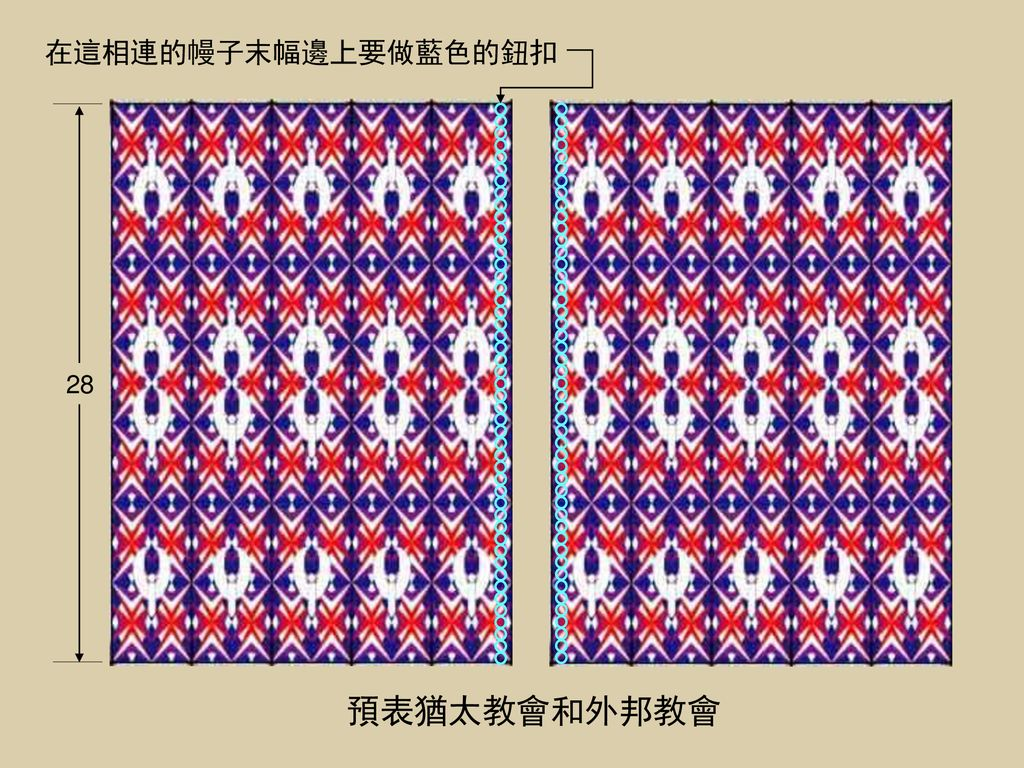
\includegraphics[width=.8\linewidth]{AMoXiFigs/chuaiji/zhangmu12}
 % \caption{A subfigure}
  \label{fig:sub1}
\end{subfigure}%
\begin{subfigure}{.5\textwidth}
  \centering
  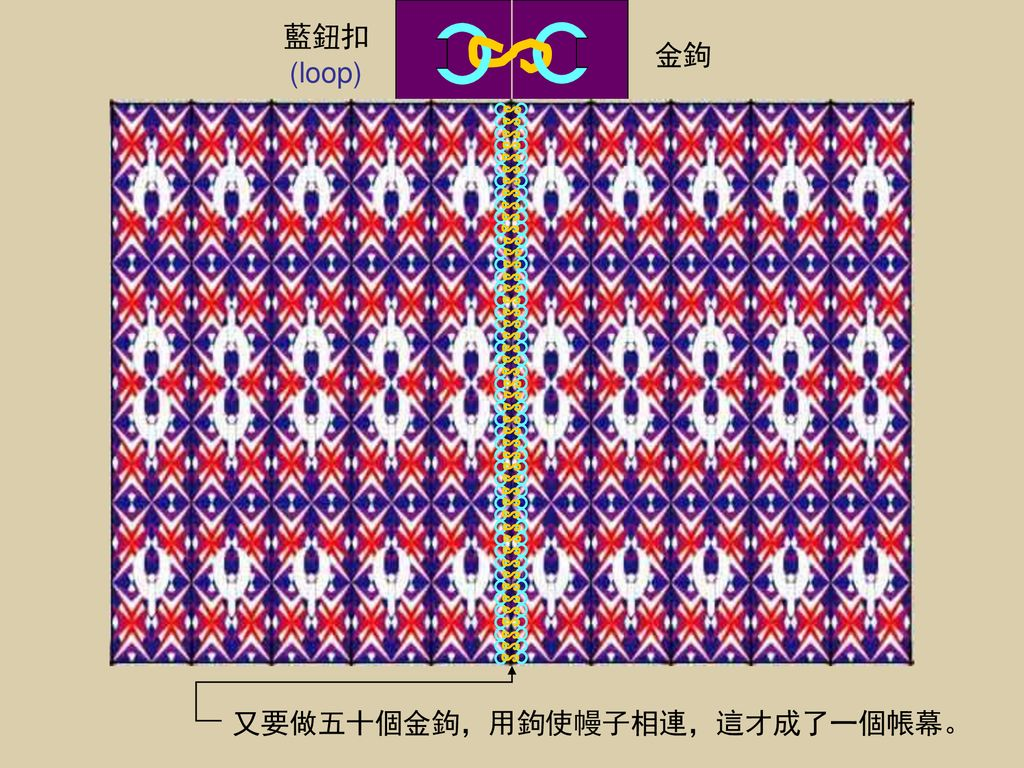
\includegraphics[width=.8\linewidth]{AMoXiFigs/chuaiji/zhangmu1}
%  \caption{A subfigure}
  \label{fig:sub2}
\end{subfigure}
\caption{幕板}
\label{fig:test}
\end{figure}

\begin{figure}[ht]
\centering
\begin{subfigure}{.5\textwidth}
  \centering
  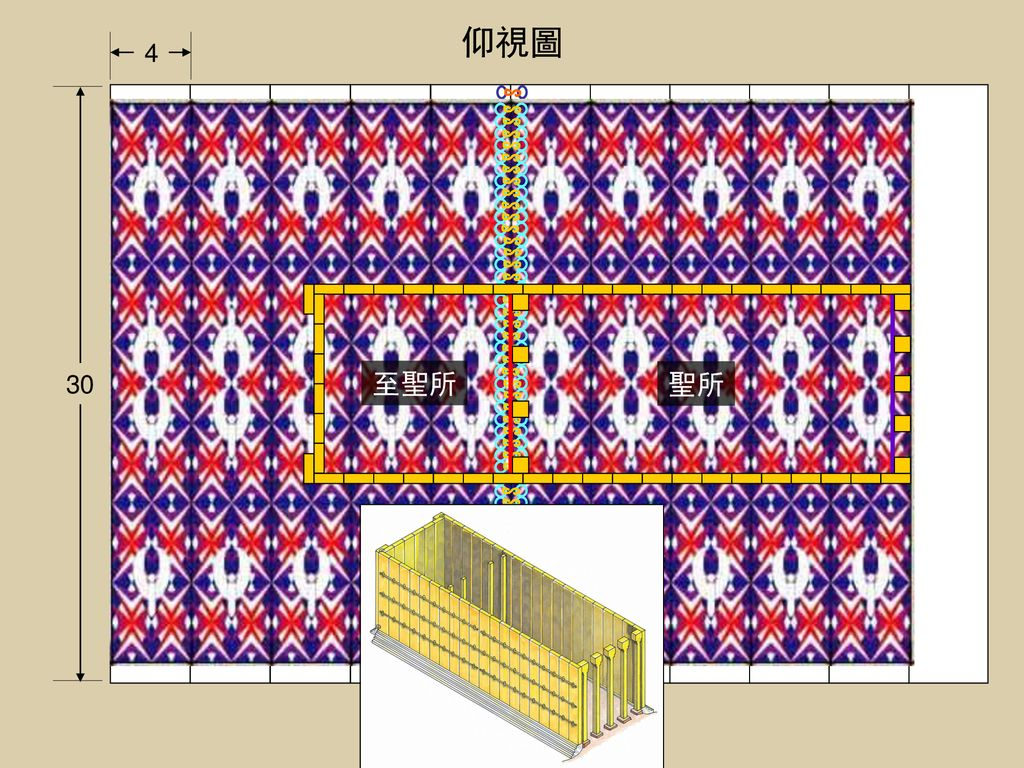
\includegraphics[width=.8\linewidth]{AMoXiFigs/chuaiji/zhangmu4}
 % \caption{A subfigure}
  \label{fig:sub1}
\end{subfigure}%
\begin{subfigure}{.5\textwidth}
  \centering
  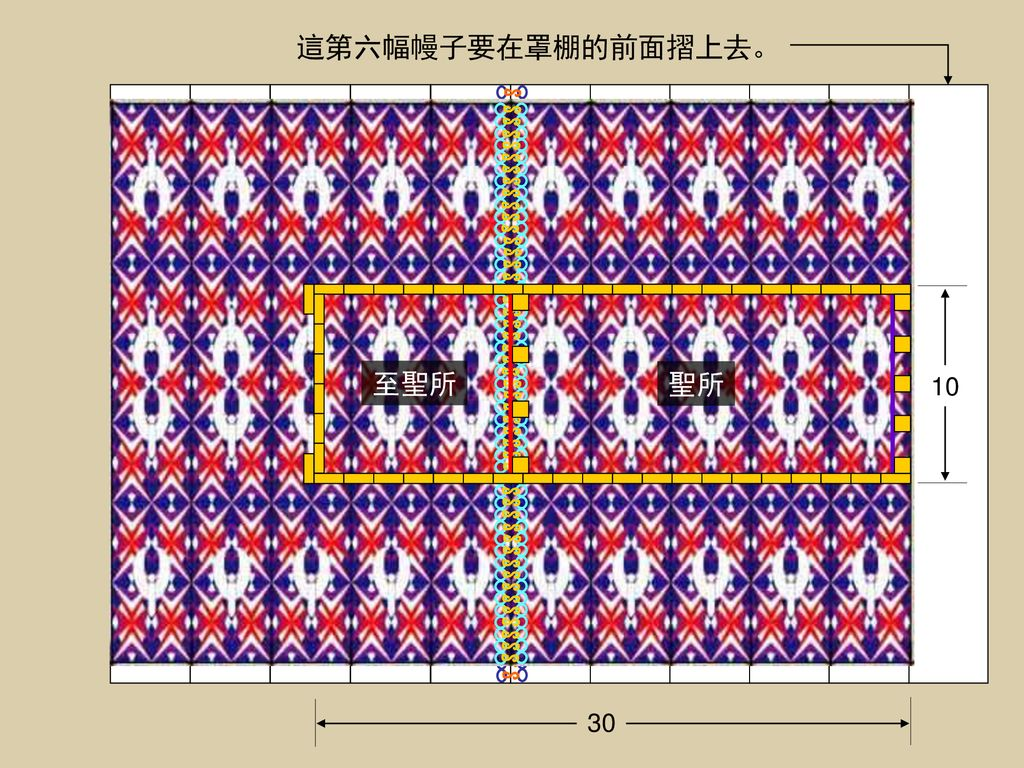
\includegraphics[width=.8\linewidth]{AMoXiFigs/chuaiji/zhangmu6}
%  \caption{A subfigure}
  \label{fig:sub2}
\end{subfigure}
\caption{幕板}
\label{fig:test}
\end{figure}
\begin{figure}[ht]
\centering
\begin{subfigure}{.5\textwidth}
  \centering
  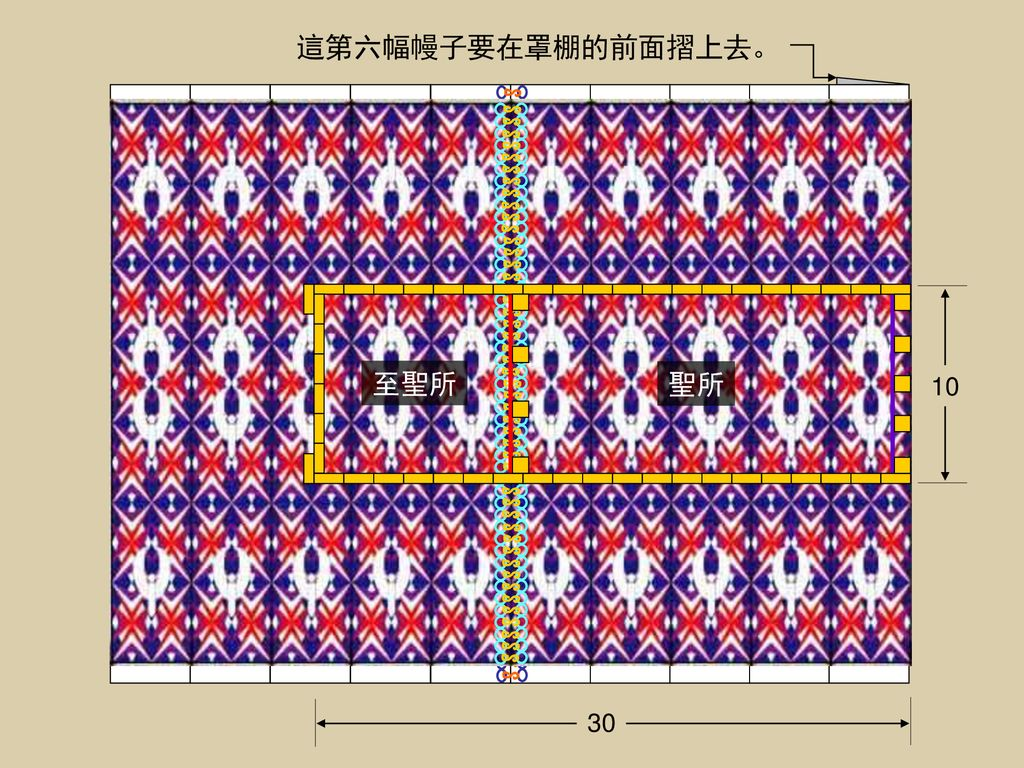
\includegraphics[width=.8\linewidth]{AMoXiFigs/chuaiji/zhangmu7}
 % \caption{A subfigure}
  \label{fig:sub1}
\end{subfigure}%
\begin{subfigure}{.5\textwidth}
  \centering
  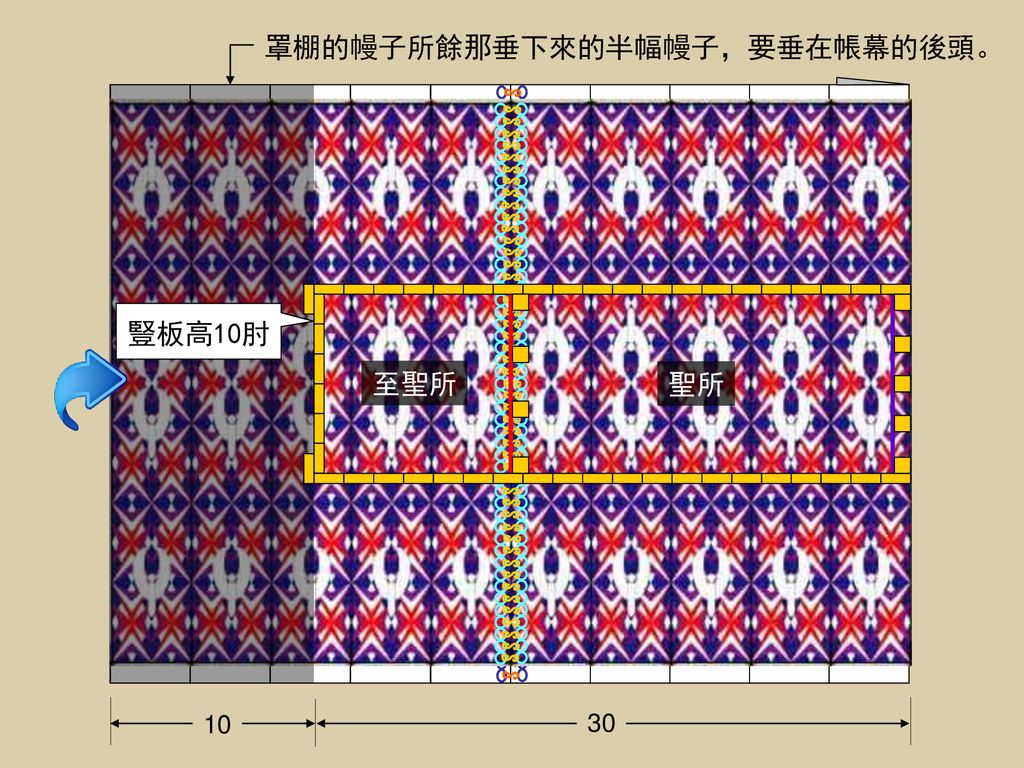
\includegraphics[width=.8\linewidth]{AMoXiFigs/chuaiji/zhangmu8}
%  \caption{A subfigure}
  \label{fig:sub2}
\end{subfigure}
\caption{幕板}
\label{fig:test}
\end{figure}
\begin{figure}[ht]
\centering
\begin{subfigure}{.5\textwidth}
  \centering
  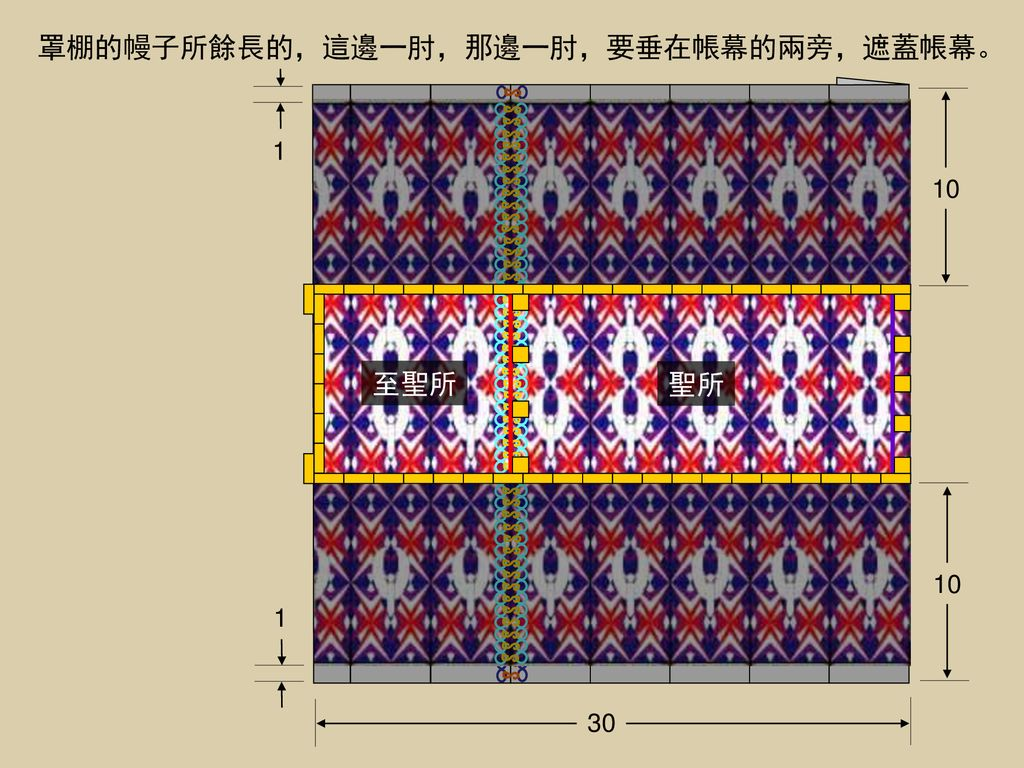
\includegraphics[width=.8\linewidth]{AMoXiFigs/chuaiji/zhangmu9}
 % \caption{A subfigure}
  \label{fig:sub1}
\end{subfigure}%
\begin{subfigure}{.5\textwidth}
  \centering
  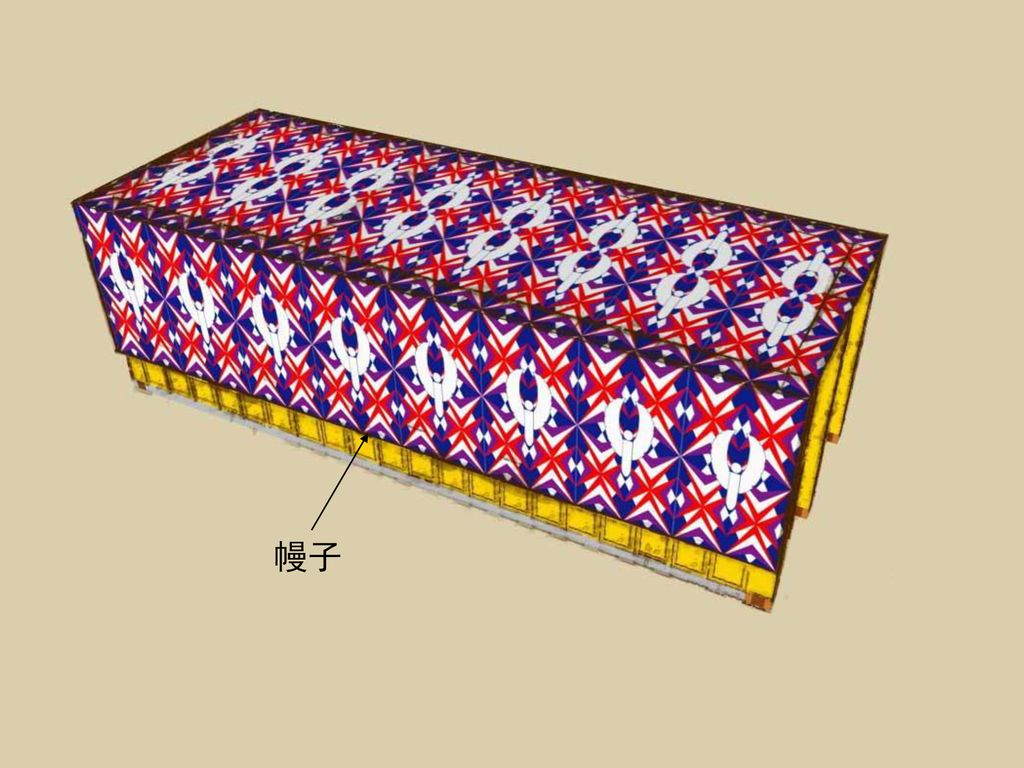
\includegraphics[width=.8\linewidth]{AMoXiFigs/chuaiji/zhangmu11}
%  \caption{A subfigure}
  \label{fig:sub2}
\end{subfigure}
\caption{幕板}
\label{fig:test}
\end{figure}



\subsubsection{造會幕的罩篷 36:14-19}
\begin{figure}[ht]
\centering
\begin{subfigure}{.5\textwidth}
  \centering
  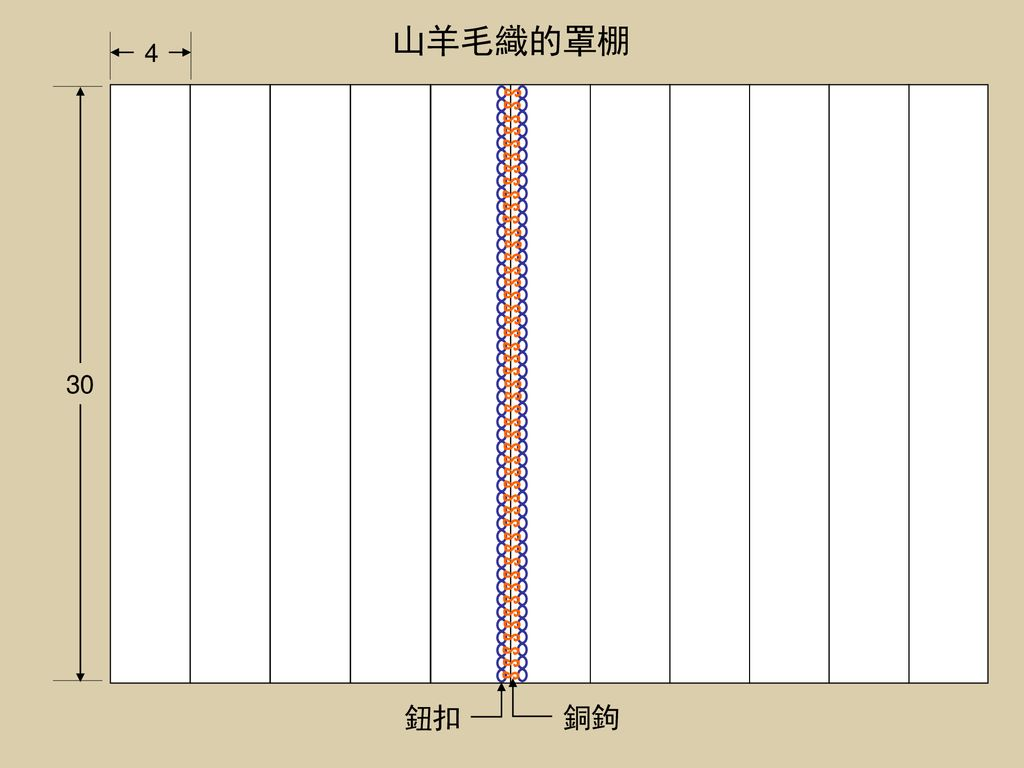
\includegraphics[width=.8\linewidth]{AMoXiFigs/chuaiji/woolcover2}
 % \caption{A subfigure}
  \label{fig:sub1}
\end{subfigure}%
\begin{subfigure}{.5\textwidth}
  \centering
  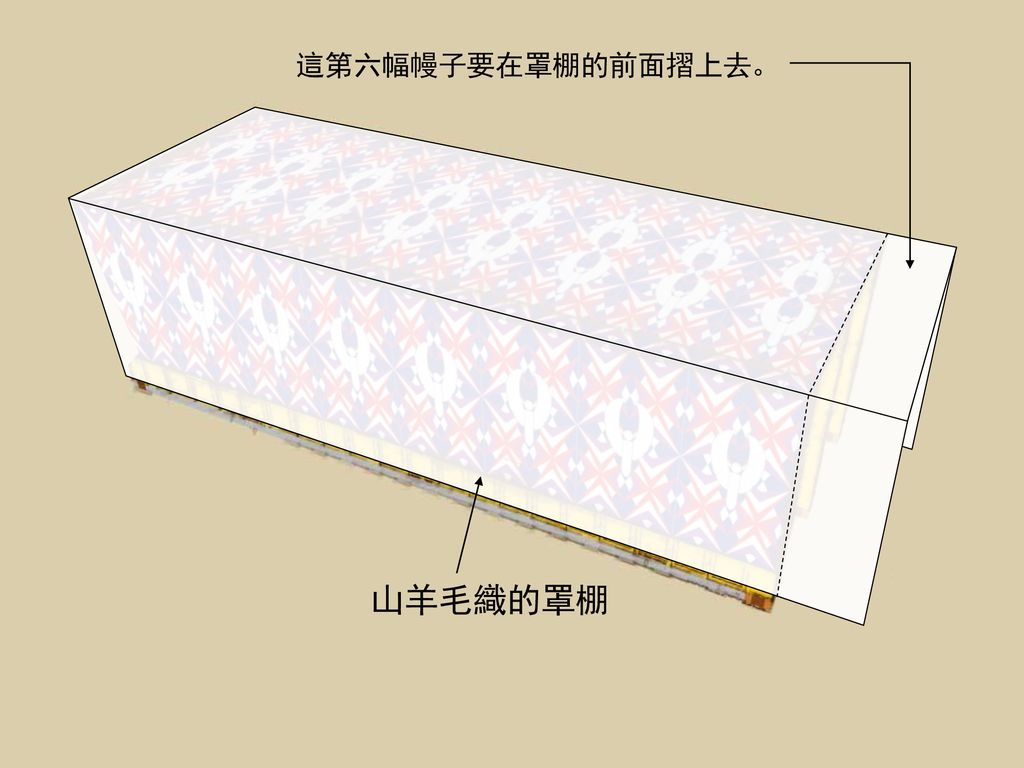
\includegraphics[width=.8\linewidth]{AMoXiFigs/chuaiji/woolcover13}
%  \caption{A subfigure}
  \label{fig:sub2}
\end{subfigure}
\caption{會幕的罩篷}
\label{fig:test}
\end{figure}

\begin{figure}[ht]
\centering
\begin{subfigure}{.5\textwidth}
  \centering
  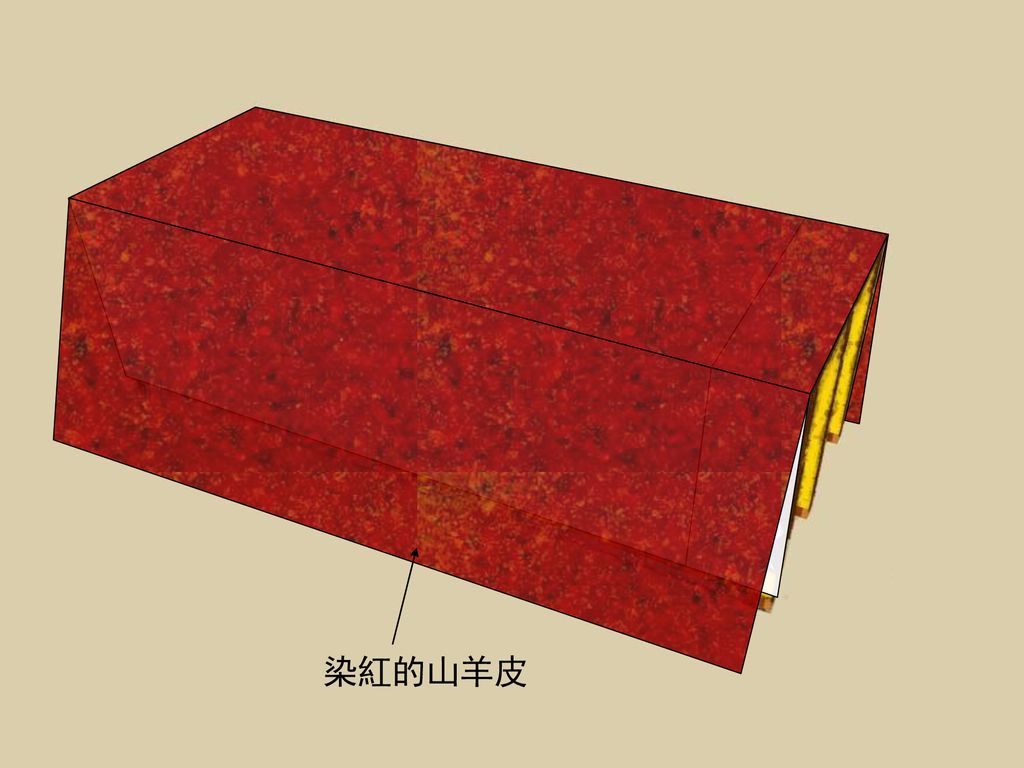
\includegraphics[width=.8\linewidth]{AMoXiFigs/chuaiji/woolcover15}
 % \caption{A subfigure}
  \label{fig:sub1}
\end{subfigure}%
\begin{subfigure}{.5\textwidth}
  \centering
  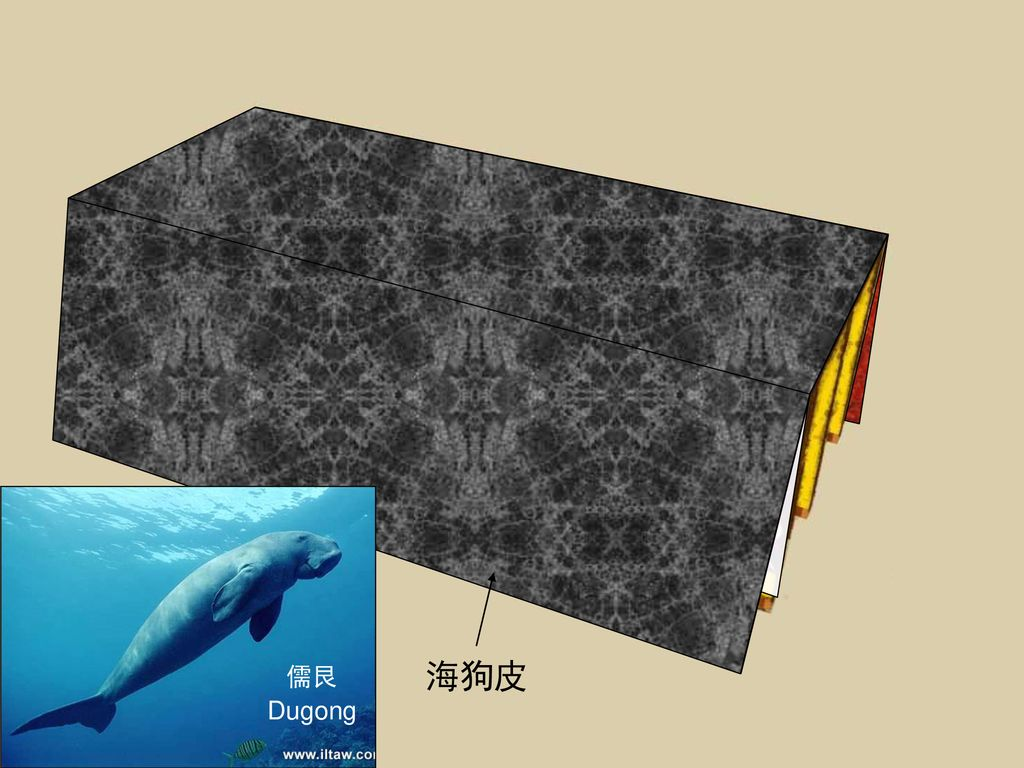
\includegraphics[width=.8\linewidth]{AMoXiFigs/chuaiji/woolcover16}
%  \caption{A subfigure}
  \label{fig:sub2}
\end{subfigure}
\caption{會幕的罩篷}
\label{fig:test}
\end{figure}

\begin{wrapfigure}{r}{0.3\textwidth}
  \centering
  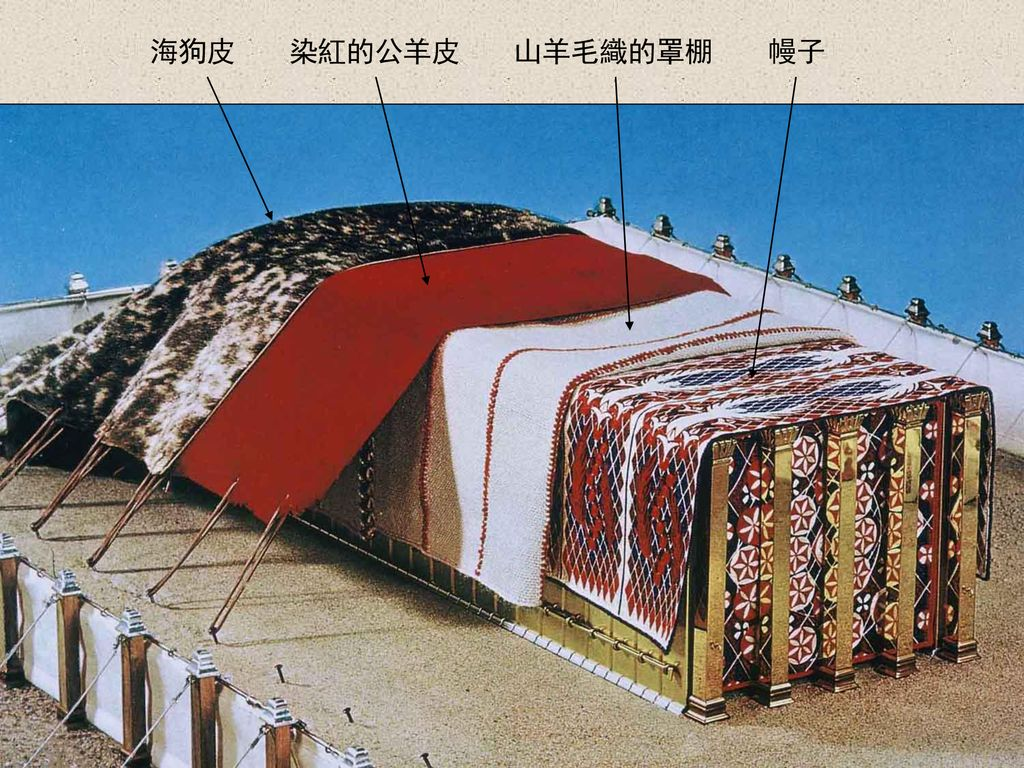
\includegraphics[width=.6\linewidth]{AMoXiFigs/chuaiji/woolcover17}
  \label{fig:sub2}
\caption{會幕的罩篷}
\label{fig:test}
\end{wrapfigure}
他用山羊毛織十一幅幔子，作為帳幕以上的罩篷。每幅幔子長三十肘，寬四肘，十一幅幔子都是一樣的尺寸。 他把五幅幔子連成一幅，又把六幅幔子連成一幅。在這相連的幔子末幅邊上做五十個紐扣，在那相連的幔子末幅邊上也做五十個紐扣。又做五十個銅鉤，使罩篷連成一個。並用染紅的公羊皮做罩篷的蓋，再用海狗皮做一層罩篷上的頂蓋。

\subsubsection{造帳幕的豎板和帶卯的銀座 36:20-34}
\begin{figure}[ht]
\centering
\hspace*{-25mm}
\begin{subfigure}{.33\textwidth}
  \centering
  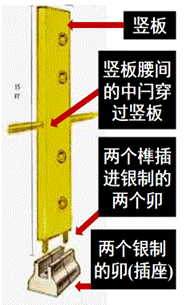
\includegraphics[width=.5\linewidth]{AMoXiFigs/chuaiji/shuban}
 % \caption{A subfigure}
  \label{fig:sub1}
\end{subfigure}%
%\hspace*{ 5mm}
\begin{subfigure}{.33\textwidth}
  \centering
  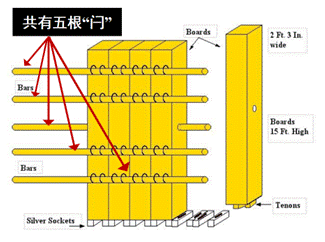
\includegraphics[width=1\linewidth]{AMoXiFigs/chuaiji/shuban1}
%  \caption{A subfigure}
  \label{fig:sub2}
\end{subfigure}
\hspace*{9mm}
\begin{subfigure}{.33\textwidth}
  \centering
  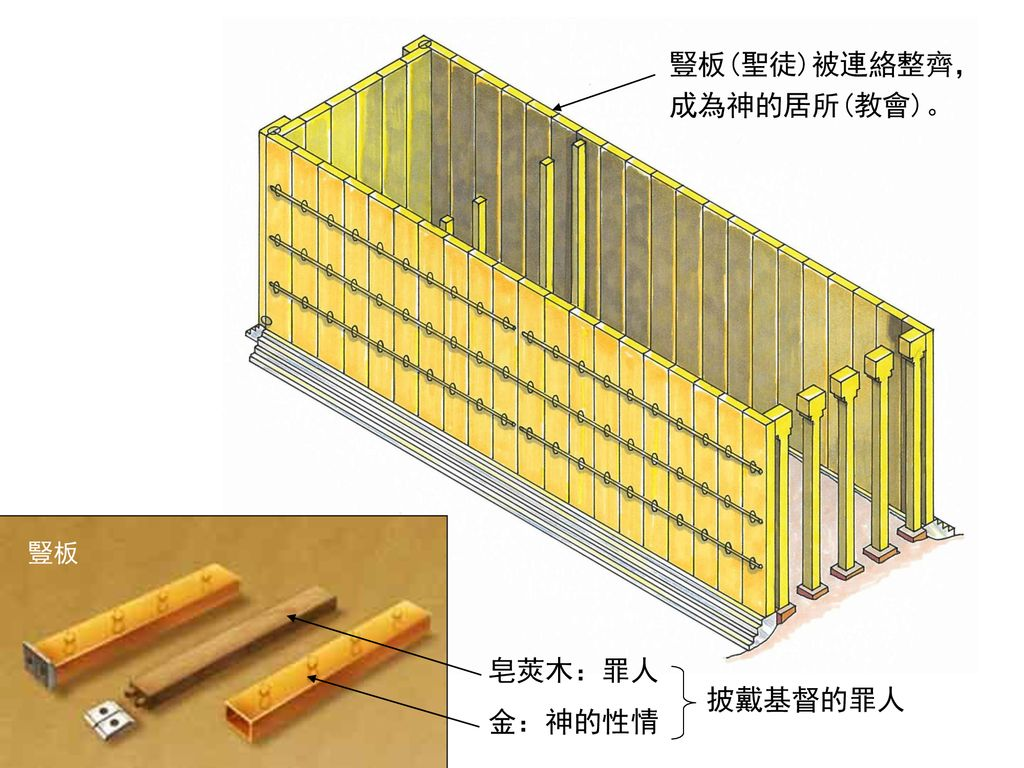
\includegraphics[width=1\linewidth]{AMoXiFigs/chuaiji/shuban2}
%  \caption{A subfigure}
  \label{fig:sub2}
\end{subfigure}
\caption{帳幕的豎板}
\label{fig:test}
\end{figure}


\begin{figure}[ht]
\centering
\begin{subfigure}{.4\textwidth}
  \centering
  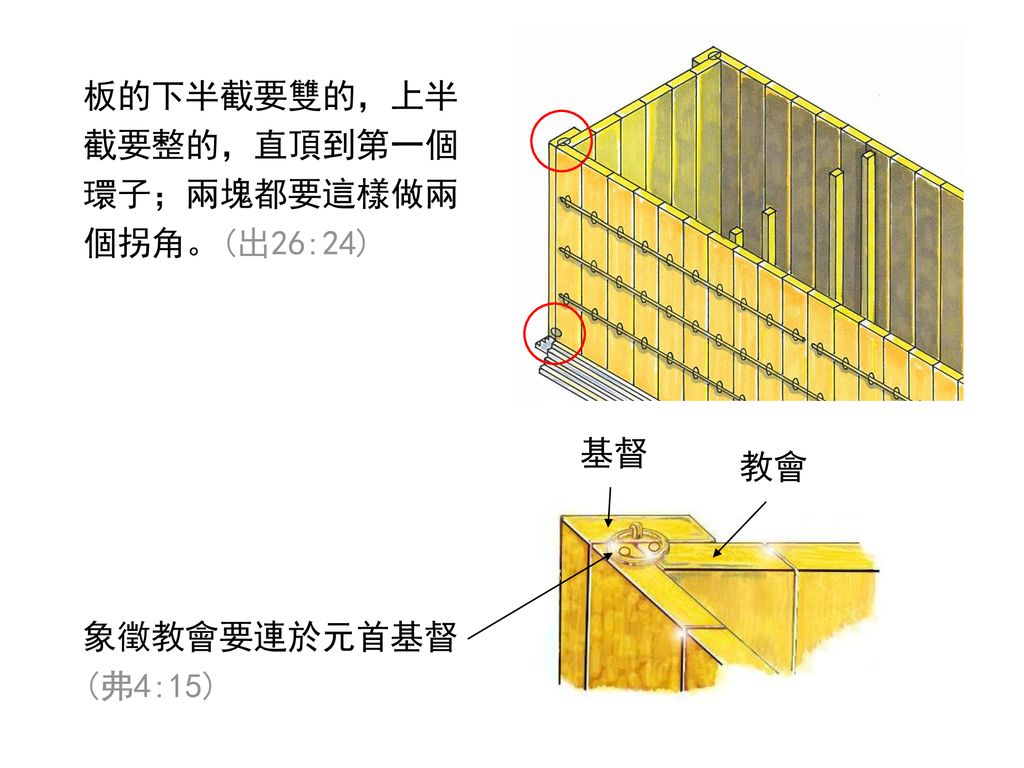
\includegraphics[width=.9\linewidth]{AMoXiFigs/chuaiji/mao}
 % \caption{A subfigure}
  \label{fig:sub1}
\end{subfigure}%
\hspace*{-20mm}
\begin{subfigure}{.4\textwidth}
  \centering
  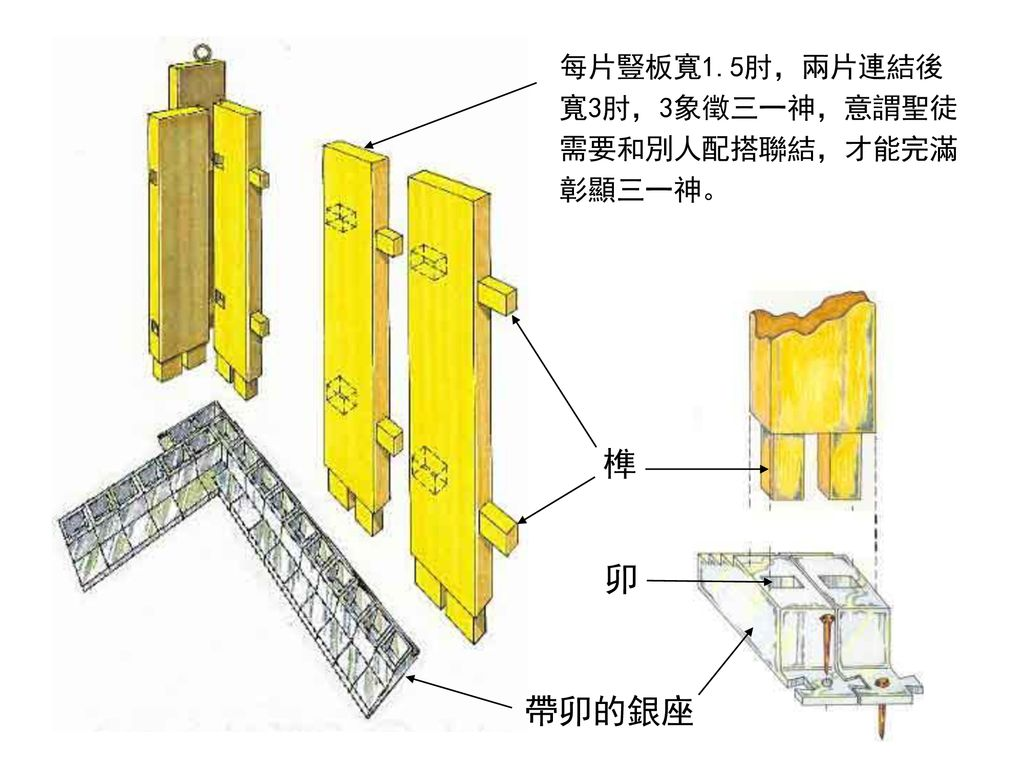
\includegraphics[width=.9\linewidth]{AMoXiFigs/chuaiji/mao3}
%  \caption{A subfigure}
  \label{fig:sub2}
\end{subfigure}
\hspace*{-20mm}
\begin{subfigure}{.4\textwidth}
  \centering
  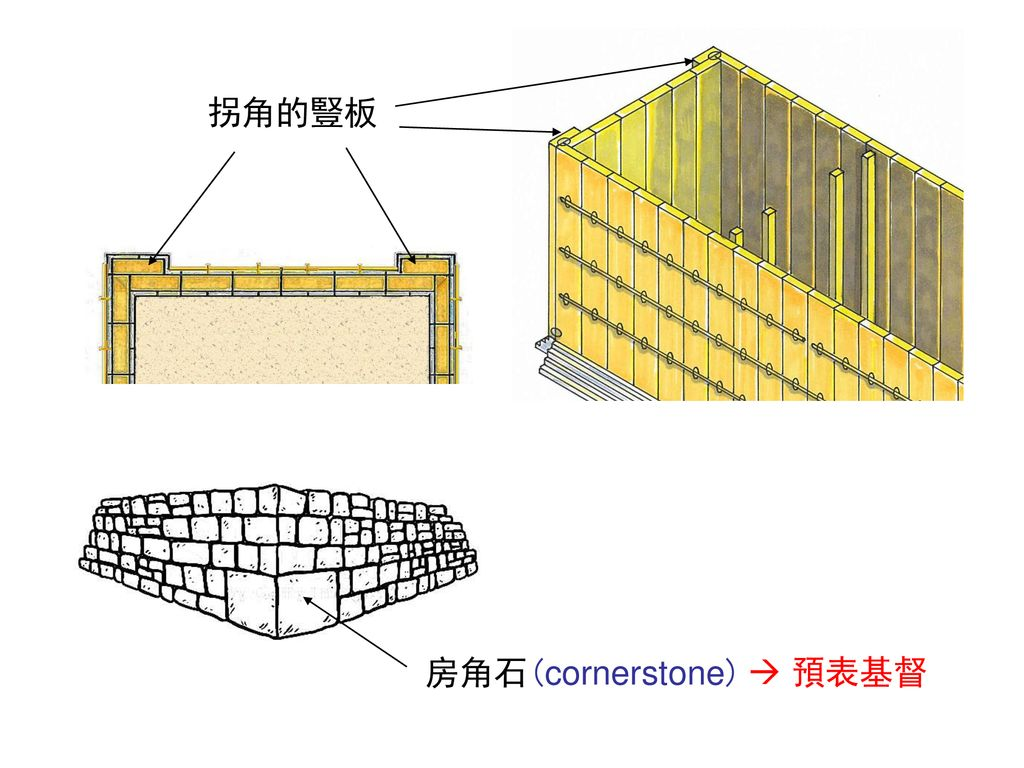
\includegraphics[width=.9\linewidth]{AMoXiFigs/chuaiji/mao5}
%  \caption{A subfigure}
  \label{fig:sub2}
\end{subfigure}
\caption{拐角的豎板}
\label{fig:test}
\end{figure}
他用皂莢木做帳幕的豎板。每塊長十肘，寬一肘半，每塊有兩榫相對。帳幕一切的板都是這樣做。帳幕的南面做板二十塊，在這二十塊板底下又做四十個帶卯的銀座，兩卯接這塊板上的兩榫，兩卯接那塊板上的兩榫。帳幕的第二面，就是北面，也做板二十塊，和帶卯的銀座四十個，這板底下有兩卯，那板底下也有兩卯。帳幕的後面，就是西面，做板六塊。\\
帳幕後面的拐角做板兩塊，板的下半截是雙的，上半截是整的，直到第一個環子，在帳幕的兩個拐角上都是這樣做。有八塊板和十六個帶卯的銀座，每塊板底下有兩卯。他用皂莢木做閂，為帳幕這面的板做五閂， 為帳幕那面的板做五閂，又為帳幕後面的板做五閂，使板腰間的中閂從這一頭通到那一頭。用金子將板包裹，又做板上的金環套閂，閂也用金子包裹。

\subsubsection{造簾 36:35-38}
\begin{wrapfigure}{r}{0.35\textwidth}
\vspace*{-17mm}
%\vspace*{-\baselineskip}
\hspace*{-25mm}
\begin{subfigure}{.5\textwidth}
  \centering
  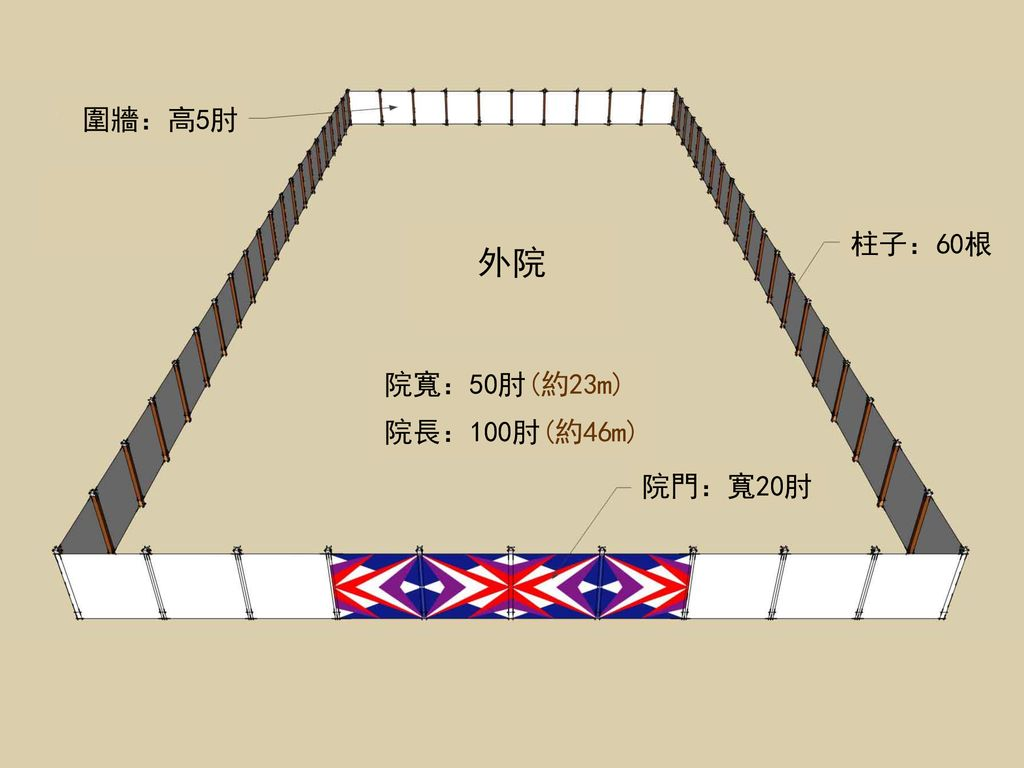
\includegraphics[width=.3\linewidth]{AMoXiFigs/chuaiji/waiyuan}
 % \caption{A subfigure}
  \label{fig:sub1}
\end{subfigure}%
\hspace*{-55mm}
\begin{subfigure}{.5\textwidth}
  \centering
   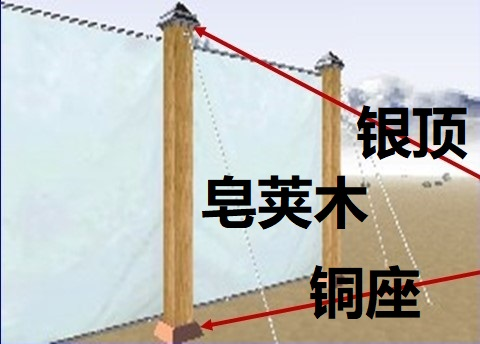
\includegraphics[width=0.32\textwidth]{AMoXiFigs/chuaiji/zhuzi1}
%  \caption{A subfigure}
  \label{fig:sub2}
\end{subfigure}

 % \begin{center}
 %   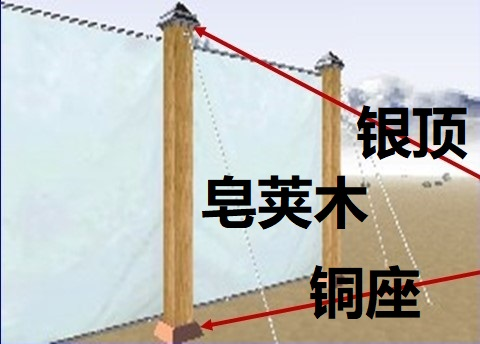
\includegraphics[width=0.16\textwidth]{AMoXiFigs/chuaiji/zhuzi1}
 % \end{center}
%\vspace*{-\baselineskip}
  \caption{簾子}
\end{wrapfigure}
他用藍色、紫色、朱紅色線和撚的細麻織幔子，以巧匠的手工繡上基路伯。為幔子做四根皂莢木柱子，用金包裹，柱子上有金鉤，又為柱子鑄了四個帶卯的銀座。拿藍色、紫色、朱紅色線和撚的細麻，用繡花的手工織帳幕的門簾，又為簾子做五根柱子和柱子上的鉤子，用金子把柱頂和柱子上的杆子包裹。柱子有五個帶卯的座，是銅的。

\subsubsection{造法櫃 37:1-9}
\begin{wrapfigure}{r}{0.35\textwidth}
\vspace*{-17mm}
\hspace*{0mm}
  \centering
  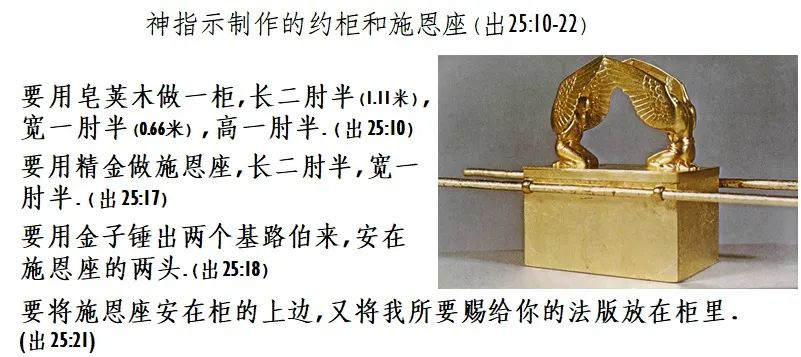
\includegraphics[width=1\linewidth]{AMoXiFigs/chuaiji/yuegui}
  \label{fig:sub1}
\vspace*{-5mm}
  \caption{法櫃 }
\end{wrapfigure}
比撒列用皂莢木做櫃，長二肘半，寬一肘半，高一肘半，裡外包上精金，四圍鑲上金牙邊。又鑄四個金環，安在櫃的四腳上，這邊兩環，那邊兩環。用皂莢木做兩根槓，用金包裹。把槓穿在櫃旁的環內，以便抬櫃。用精金做施恩座，長二肘半，寬一肘半。用金子錘出兩個基路伯來，安在施恩座的兩頭，這頭做一個基路伯，那頭做一個基路伯，二基路伯接連一塊，在施恩座的兩頭。二基路伯高張翅膀，遮掩施恩座，基路伯是臉對臉，朝著施恩座。

\subsubsection{造桌 37:10-16}
他用皂莢木做一張桌子，長二肘，寬一肘，高一肘半，又包上精金，四圍鑲上金牙邊。桌子的四圍各做一掌寬的橫梁，橫梁上鑲著金牙邊。又鑄了四個金環，安在桌子四腳的四角上。安環子的地方是挨近橫梁，可以穿槓抬桌子。他用皂莢木做兩根槓，用金包裹，以便抬桌子。又用精金做桌子上的器皿，就是盤子，調羹，並奠酒的瓶和爵。

\subsubsection{造燈臺 37:17-24}
\begin{wrapfigure}{r}{0.18\textwidth}
\vspace*{-10mm}
%\vspace*{-\baselineskip}
  \begin{center}
    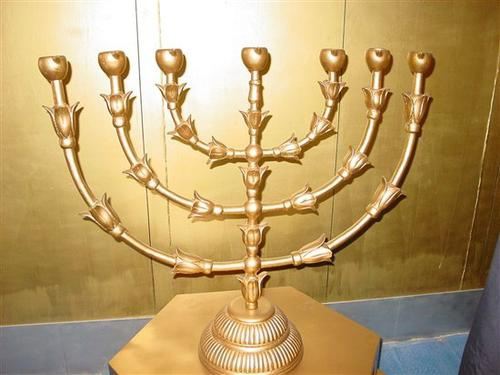
\includegraphics[width=0.18\textwidth]{AMoXiFigs/chuaiji/jindengtai}
  \end{center}
\vspace*{-2mm}
  \caption{燈臺}
\end{wrapfigure}
他用精金做一個燈臺，這燈臺的座和幹與杯、球、花，都是接連一塊錘出來的。燈臺兩旁杈出六個枝子，這旁三個，那旁三個。這旁每枝上有三個杯，形狀像杏花，有球有花；那旁每枝上也有三個杯，形狀像杏花，有球有花。從燈臺杈出來的六個枝子都是如此。 燈臺上有四個杯，形狀像杏花，有球有花。燈臺每兩個枝子以下有球，與枝子接連一塊，燈臺杈出的六個枝子都是如此。球和枝子是接連一塊，都是一塊精金錘出來的。用精金做燈臺的七個燈盞，並燈臺的蠟剪和蠟花盤。他用精金一他連得做燈臺和燈臺的一切器具。

\subsubsection{造香壇 37:25-29}
他用皂莢木做香壇，是四方的，長一肘，寬一肘，高二肘，壇的四角與壇接連一塊。又用精金把壇的上面與壇的四面並壇的四角包裹，又在壇的四圍鑲上金牙邊。做兩個金環，安在牙子邊以下，在壇的兩旁兩根橫撐上，作為穿槓的用處，以便抬壇。用皂莢木做槓，用金包裹。又按做香之法做聖膏油和馨香料的淨香。

\subsubsection{造祭壇 38:1-7}
\begin{wrapfigure}{r}{0.7\textwidth}
\vspace*{-5mm}
%\begin{figure}[ht]
\centering
\begin{subfigure}{.5\textwidth}
  \centering
  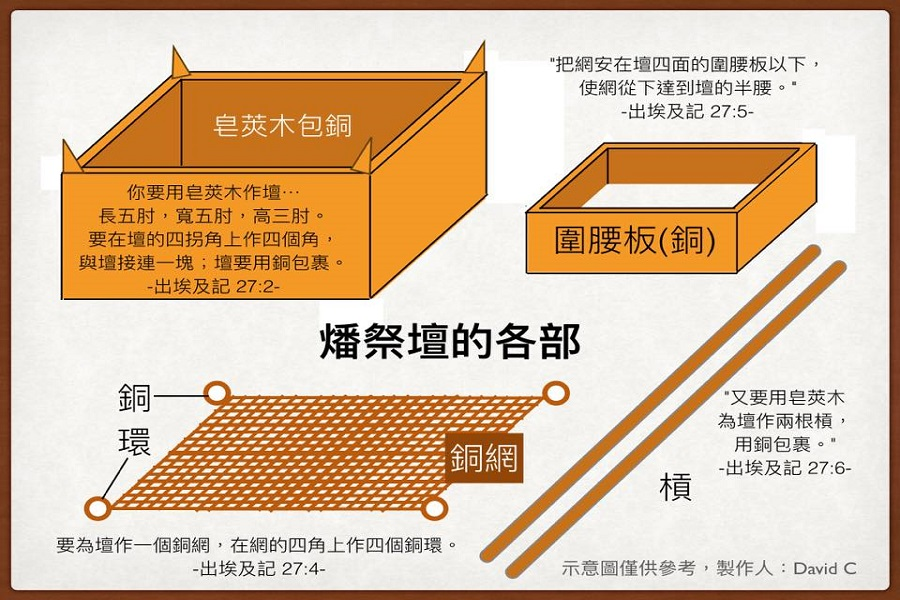
\includegraphics[width=.7\linewidth]{AMoXiFigs/chuaiji/jitan}
 % \caption{A subfigure}
  \label{fig:sub1}
\end{subfigure}%
\hspace*{-30mm}
\begin{subfigure}{.5\textwidth}
  \centering
  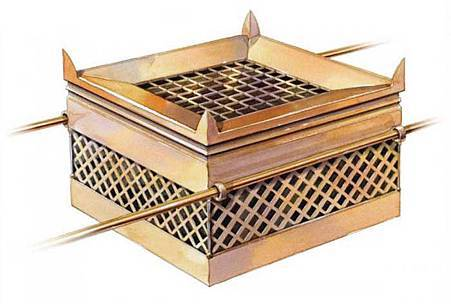
\includegraphics[width=.6\linewidth]{AMoXiFigs/chuaiji/jitan3}
%  \caption{A subfigure}
  \label{fig:sub2}
\end{subfigure}
\caption{祭壇}
\label{fig:test}
\end{wrapfigure}
他用皂莢木做燔祭壇，是四方的，長五肘，寬五肘，高三肘。在壇的四拐角上做四個角，與壇接連一塊，用銅把壇包裹。他做壇上的盆、鏟子、盤子、肉叉子、火鼎，這一切器具都是用銅做的。又為壇做一個銅網，安在壇四面的圍腰板以下，從下達到壇的半腰。為銅網的四角鑄四個環子，作為穿槓的用處。 用皂莢木做槓，用銅包裹，把槓穿在壇兩旁的環子內，用以抬壇；並用板做壇，壇是空的。

\subsubsection{造浴盆 38:8}
他用銅做洗濯盆和盆座，是用會幕門前伺候的婦人之鏡子做的。

\subsubsection{立幕院 38:9-20}

他做帳幕的院子。院子的南面用撚的細麻做帷子，寬一百肘。帷子的柱子二十根，帶卯的銅座二十個，柱子上的鉤子和杆子都是用銀子做的。北面也有帷子，寬一百肘。帷子的柱子二十根，帶卯的銅座二十個，柱子上的鉤子和杆子都是用銀子做的。院子的西面有帷子，寬五十肘。帷子的柱子十根，帶卯的座十個，柱子的鉤子和杆子都是用銀子做的。院子的東面，寬五十肘。門這邊的帷子十五肘，那邊也是一樣。帷子的柱子三根，帶卯的座三個。在門的左右各有帷子十五肘，帷子的柱子三根，帶卯的座三個。院子四面的帷子都是用撚的細麻做的。柱子帶卯的座是銅的，柱子上的鉤子和杆子是銀的，柱頂是用銀子包的。院子一切的柱子都是用銀杆連絡的。院子的門簾是以繡花的手工，用藍色、紫色、朱紅色線和撚的細麻織的，寬二十肘，高五肘，與院子的帷子相配。帷子的柱子四根，帶卯的銅座四個，柱子上的鉤子和杆子是銀的，柱頂是用銀子包的。帳幕一切的橛子和院子四圍的橛子都是銅的。

\subsubsection{核記民獻金銀銅之數 38:21-31}

這是法櫃的帳幕中利未人所用物件的總數，是照摩西的吩咐，經祭司亞倫的兒子以他瑪的手數點的。凡耶和華所吩咐摩西的，都是猶大支派戶珥的孫子、烏利的兒子比撒列做的。與他同工的有但支派中亞希撒抹的兒子亞何利亞伯，他是雕刻匠，又是巧匠，又能用藍色、紫色、朱紅色線和細麻繡花。

\begin{wraptable}{r}{14.5cm}
%\begin{table}[H]
\vspace*{-\baselineskip}
\center
\begin{tabular}{ c c l }
\toprule
材料 &重量 &用途\\\hline
所獻的金子&29他連得730舍客勒 &  \\\hline
被數人所出的銀子&100他連得 &100帶卯的座,1他連得/帶卯的座\\
0.5舍客勒/被數人 &1775舍客勒&做柱子上的鉤子，包裹柱頂並柱子上的杆子\\\hline
銅 &70他連得2400舍客勒&會幕門帶卯的座,銅壇並壇上的銅網並一切器具\\
   &                               &院子四圍,院門帶卯的座,帳幕和院子四圍的橛子\\\hline
\end{tabular}
\caption{技工比撒列,亞何利亞伯}
%\end{table} 
\end{wraptable}
為聖所一切工作使用所獻的\textcolor{blue}{金子}，按聖所的平，有二十九他連得並七百三十舍客勒。會中被數的人所出的\textcolor{blue}{銀子}，按聖所的平，有一百他連得並一千七百七十五舍客勒。凡過去歸那些被數之人的，從二十歲以外，有六十萬零三千五百五十人，按聖所的平，每人出銀半舍客勒，就是一比加。用那一百他連得銀子鑄造聖所帶卯的座和幔子柱子帶卯的座，一百他連得共一百帶卯的座，每帶卯的座用一他連得。用那一千七百七十五舍客勒銀子做柱子上的鉤子，包裹柱頂並柱子上的杆子。所獻的\textcolor{blue}{銅}有七十他連得並二千四百舍客勒。 用這銅做會幕門帶卯的座和銅壇，並壇上的銅網和壇的一切器具，並院子四圍帶卯的座和院門帶卯的座，與帳幕一切的橛子和院子四圍所有的橛子。

\subsubsection{造會幕所用的金屬 39:1-7}
比撒列用藍色、紫色、朱紅色線做精緻的衣服，在聖所用以供職，又為亞倫做聖衣，是照耶和華所吩咐摩西的。他用金線和藍色、紫色、朱紅色線並撚的細麻做以弗得。把金子錘成薄片，剪出線來，與藍色、紫色、朱紅色線，用巧匠的手工一同繡上。又為以弗得做兩條相連的肩帶，接連在以弗得的兩頭。其上巧工織的帶子和以弗得一樣的做法，用以束上，與以弗得接連一塊，是用金線和藍色、紫色、朱紅色線並撚的細麻做的，是照耶和華所吩咐摩西的。
又琢出兩塊紅瑪瑙，鑲在金槽上，彷彿刻圖書，按著以色列兒子的名字雕刻，將這兩塊寶石安在以弗得的兩條肩帶上，為以色列人做紀念石，是照耶和華所吩咐摩西的。

\subsubsection{做胸牌 39:8-21}
他用巧匠的手工做胸牌，和以弗得一樣的做法，用金線與藍色、紫色、朱紅色線並撚的細麻做的。胸牌是四方的，疊為兩層，這兩層長一虎口，寬一虎口，上面鑲著寶石四行：第一行是紅寶石、紅璧璽、紅玉， 第二行是綠寶石、藍寶石、金鋼石，第三行是紫瑪瑙、白瑪瑙、紫晶，第四行是水蒼玉、紅瑪瑙、碧玉。這都鑲在金槽中。 14 這些寶石都是按著以色列十二個兒子的名字，彷彿刻圖書，刻十二個支派的名字。在胸牌上，用精金擰成如繩子的鏈子。又做兩個金槽和兩個金環，安在胸牌的兩頭。 把那兩條擰成的金鏈子穿過胸牌兩頭的環子，又把鏈子的那兩頭接在兩槽上，安在以弗得前面肩帶上。做兩個金環，安在胸牌的兩頭，在以弗得裡面的邊上。 又做兩個金環，安在以弗得前面兩條肩帶的下邊，挨近相接之處，在以弗得巧工織的帶子以上。用一條藍細帶子把胸牌的環子和以弗得的環子繫住，使胸牌貼在以弗得巧工織的帶子上，不可與以弗得離縫，是照耶和華所吩咐摩西的。

\subsubsection{做外袍 39:22-26}
他用織工做以弗得的外袍，顏色全是藍的。袍上留一領口，口的周圍織出領邊來，彷彿鎧甲的領口，免得破裂。在袍子底邊上，用藍色、紫色、朱紅色線並撚的細麻做石榴。又用精金做鈴鐺，把鈴鐺釘在袍子周圍底邊上的石榴中間：一個鈴鐺，一個石榴，一個鈴鐺，一個石榴，在袍子周圍底邊上，用以供職，是照耶和華所吩咐摩西的。

\subsubsection{做內袍 39:27-29}
他用織成的細麻布為亞倫和他的兒子做內袍，並用細麻布做冠冕和華美的裹頭巾，用撚的細麻布做褲子，又用藍色、紫色、朱紅色線並撚的細麻，以繡花的手工做腰帶，是照耶和華所吩咐摩西的。

\subsubsection{造冕牌 39:30-31}
他用精金做聖冠上的牌，在上面按刻圖書之法，刻著：歸耶和華為聖。又用一條藍細帶子將牌繫在冠冕上，是照耶和華所吩咐摩西的。

%\subsection{造會幕竣工 36:8-39:31}
\subsubsection{幕工告竣 39:32-43}
帳幕，就是會幕，一切的工就這樣做完了。凡耶和華所吩咐摩西的，以色列人都照樣做了。他們送到摩西那裡，帳幕和帳幕的一切器具，就是鉤子、板、閂、柱子、帶卯的座，染紅公羊皮的蓋、海狗皮的頂蓋和遮掩櫃的幔子，法櫃和櫃的槓並施恩座，桌子和桌子的一切器具並陳設餅， 精金的燈臺和擺列的燈盞與燈臺的一切器具並點燈的油， 金壇，膏油，馨香的香料，會幕的門簾，銅壇和壇上的銅網，壇的槓並壇的一切器具，洗濯盆和盆座，院子的帷子和柱子，並帶卯的座，院子的門簾、繩子、橛子，並帳幕和會幕中一切使用的器具，精工做的禮服和祭司亞倫並他兒子在聖所用以供祭司職分的聖衣。這一切工作都是以色列人照耶和華所吩咐摩西做的。耶和華怎樣吩咐的，他們就怎樣做了。摩西看見一切的工都做成了，就給他們祝福


\subsubsection{命摩西建會幕 40:1-16}
耶和華曉諭摩西說： 「正月初一日，你要立起帳幕，把法櫃安放在裡面，用幔子將櫃遮掩。把桌子搬進去，擺設上面的物。把燈臺搬進去，點其上的燈。把燒香的金壇安在法櫃前，掛上帳幕的門簾。把燔祭壇安在帳幕門前。把洗濯盆安在會幕和壇的中間，在盆裡盛水。又在四圍立院帷，把院子的門簾掛上。 用膏油把帳幕和其中所有的都抹上，使帳幕和一切器具成聖，就都成聖。又要抹燔祭壇和一切器具，使壇成聖，就都成為至聖。要抹洗濯盆和盆座，使盆成聖。要使亞倫和他兒子到會幕門口來，用水洗身。要給亞倫穿上聖衣，又膏他，使他成聖，可以給我供祭司的職分。又要使他兒子來，給他們穿上內袍。怎樣膏他們的父親，也要照樣膏他們，使他們給我供祭司的職分。他們世世代代凡受膏的，就永遠當祭司的職任。」摩西這樣行，都是照耶和華所吩咐他的。


\subsubsection{會幕完工 40:17-33 }
第二年正月初一日，帳幕就立起來。摩西立起帳幕，安上帶卯的座，立上板，穿上閂，立起柱子，在帳幕以上搭罩篷，把罩篷的頂蓋蓋在其上，是照耶和華所吩咐他的。又把法版放在櫃裡，把槓穿在櫃的兩旁，把施恩座安在櫃上。把櫃抬進帳幕，掛上遮掩櫃的幔子，把法櫃遮掩了，是照耶和華所吩咐他的。又把桌子安在會幕內，在帳幕北邊，在幔子外，在桌子上將餅陳設在耶和華面前，是照耶和華所吩咐他的。又把燈臺安在會幕內，在帳幕南邊，與桌子相對，在耶和華面前點燈，是照耶和華所吩咐他的。把金壇安在會幕內的幔子前，在壇上燒了馨香料做的香，是照耶和華所吩咐他的。又掛上帳幕的門簾。在會幕的帳幕門前，安設燔祭壇，把燔祭和素祭獻在其上，是照耶和華所吩咐他的。把洗濯盆安在會幕和壇的中間，盆中盛水，以便洗濯。摩西和亞倫並亞倫的兒子在這盆裡洗手洗腳。他們進會幕或就近壇的時候，便都洗濯，是照耶和華所吩咐他的。在帳幕和壇的四圍立了院帷，把院子的門簾掛上。這樣，摩西就完了工。

\subsubsection{神的榮光在會幕顯現 40:34-38 （民9:15-23 ）}
當時，雲彩遮蓋會幕，耶和華的榮光就充滿了帳幕。摩西不能進會幕，因為雲彩停在其上，並且耶和華的榮光充滿了帳幕。每逢雲彩從帳幕收上去，以色列人就起程前往；雲彩若不收上去，他們就不起程，直等到雲彩收上去。日間，耶和華的雲彩是在帳幕以上；夜間，雲中有火，在以色列全家的眼前。在他們所行的路上，都是這樣。




















\include{AMoXiFiles/LiWeiJi}
\chapter{民數記}

\section{在西乃的末期 1-10}

\subsection{數點以色列人，各支派依序安營 1:1－2:31}
\subsubsection{核以色列族能臨陣男丁之總數 1:1-3}
以色列人出埃及地後，第二年二月初一日，耶和華在西奈的曠野，會幕中曉諭摩西說：「你要按以色列全會眾的家室、宗族，人名的數目，計算所有的男丁。凡以色列中，從二十歲以外，能出去打仗的，你和亞倫要照他們的軍隊數點。

\subsubsection{派定各族族長 1:4-19}
每支派中，必有一人做本支派的族長，幫助你們。他們的名字：屬\textcolor{blue}{魯本}的，有示丟珥的兒子以利蓿；屬\textcolor{blue}{西緬}的，有蘇利沙代的兒子示路蔑；屬\textcolor{blue}{猶大}的，有亞米拿達的兒子拿順；屬\textcolor{blue}{以薩迦}的，有蘇押的兒子拿坦業；屬\textcolor{blue}{西布倫}的，有希倫的兒子以利押；\textcolor{blue}{約瑟}子孫屬\textcolor{blue}{以法蓮}的，有亞米忽的兒子以利沙瑪；屬\textcolor{blue}{瑪拿西}的，有比大蓿的兒子迦瑪列；屬\textcolor{blue}{便雅憫}的，有基多尼的兒子亞比但；屬\textcolor{blue}{但}的，有亞米沙代的兒子亞希以謝； 屬\textcolor{blue}{亞設}的，有俄蘭的兒子帕結；屬\textcolor{blue}{迦得}的，有丟珥的兒子以利雅薩；屬\textcolor{blue}{拿弗他利}的，有以南的兒子亞希拉。這都是從會中選召的，各做本支派的首領，都是以色列軍中的統領。」於是摩西、亞倫帶著這些按名指定的人，當二月初一日招聚全會眾。會眾就照他們的家室、宗族，人名的數目，從二十歲以外的，都述說自己的家譜。耶和華怎樣吩咐摩西，他就怎樣在西奈的曠野數點他們。

\subsubsection{以色列族被统计的男丁總數 1:20-46}
\begin{wraptable}{r}{10.cm}
\vspace*{-8mm}
\centering
\begin{tabular}{c|c|c|c|c|c}\hline\hline
支派  & 首領名字&  父親名字 &第一次&第二次 &增减\\\hline
流便  &以利蓿 & 示丟珥&46,500 & &\\
西緬  & 示路蔑 &  蘇利沙代&59,300 & & \\
猶大 & 拿順 &亞米拿達&74,600 & &\\
以薩迦 &拿坦業  & 蘇押&54,400 & & \\
西布倫&  以利押& 希倫&57,400 & & \\
以法蓮  &以利沙瑪 & 亞米忽&40,500 & &\\
瑪拿西  & 迦瑪列 &  比大蓿&32,200 & & \\
便雅憫 &亞比但 &基多尼&35,400 && \\
但  &亞希以謝 & 亞米沙代&62,700 && \\
亞設  & 帕結 &  俄蘭&41,500 & & \\
迦得&以利雅薩 & 丟珥&45,650 & & \\
拿弗他利&亞希拉 & 以南&53,400 & & \\\hline
總數&&&603,550&&\\\hline
\end{tabular}
\caption{以色列族被统计的男丁總數}
\end{wraptable}
以色列的長子魯本子孫的後代，照著家室、宗族，人名的數目，從二十歲以外，凡能出去打仗，被數的男丁共有四萬六千五百名。西緬子孫的後代，照著家室、宗族，人名的數目，從二十歲以外，凡能出去打仗，被數的男丁共有五萬九千三百名。迦得子孫的後代，照著家室、宗族，人名的數目，從二十歲以外，凡能出去打仗，被數的共有四萬五千六百五十名。猶大子孫的後代，照著家室、宗族，人名的數目，從二十歲以外，凡能出去打仗，被數的共有七萬四千六百名。以薩迦子孫的後代，照著家室、宗族，人名的數目，從二十歲以外，凡能出去打仗，被數的共有五萬四千四百名。西布倫子孫的後代，照著家室、宗族，人名的數目，從二十歲以外，凡能出去打仗，被數的共有五萬七千四百名。約瑟子孫，屬以法蓮子孫的後代，照著家室、宗族，人名的數目，從二十歲以外，凡能出去打仗，被數的共有四萬零五百名。 瑪拿西子孫的後代，照著家室、宗族，人名的數目，從二十歲以外，凡能出去打仗，被數的共有三萬二千二百名。便雅憫子孫的後代，照著家室、宗族，人名的數目，從二十歲以外，凡能出去打仗，被數的共有三萬五千四百名。但子孫的後代，照著家室、宗族，人名的數目，從二十歲以外，凡能出去打仗，被數的共有六萬二千七百名。亞設子孫的後代，照著家室、宗族，人名的數目，從二十歲以外，凡能出去打仗，被數的共有四萬一千五百名。拿弗他利子孫的後代，照著家室、宗族，人名的數目，從二十歲以外，凡能出去打仗，被數的共有五萬三千四百名。這些就是被數點的，是摩西、亞倫和以色列中十二個首領所數點的，這十二個人各做各宗族的代表。這樣，凡以色列人中被數的，照著宗族從二十歲以外，能出去打仗，被數的共有六十萬零三千五百五十名。

\subsubsection{利未支派不列其數 1:47-54}
利未人卻沒有按著支派數在其中， 48 因為耶和華曉諭摩西說： 49 「唯獨利未支派你不可數點，也不可在以色列人中計算他們的總數。 50 只要派利未人管法櫃的帳幕和其中的器具，並屬乎帳幕的。他們要抬(搬運)帳幕和其中的器具，並要辦理帳幕的事，在帳幕的四圍安營。 51 帳幕將往前行的時候，利未人要拆卸；將支搭的時候，利未人要豎起。近前來的外人必被治死。 52 以色列人支搭帳篷，要照他們的軍隊，各歸本營，各歸本纛。 53 但利未人要在法櫃帳幕的四圍安營，免得憤怒臨到以色列會眾。利未人並要謹守法櫃的帳幕。」 54 以色列人就這樣行。凡耶和華所吩咐摩西的，他們就照樣行了。


\subsubsection{東邊支派首領及安營之所 2:1-8}
\begin{wrapfigure}{r}{0.5\textwidth}
\vspace*{-22mm}
\begin{center} 
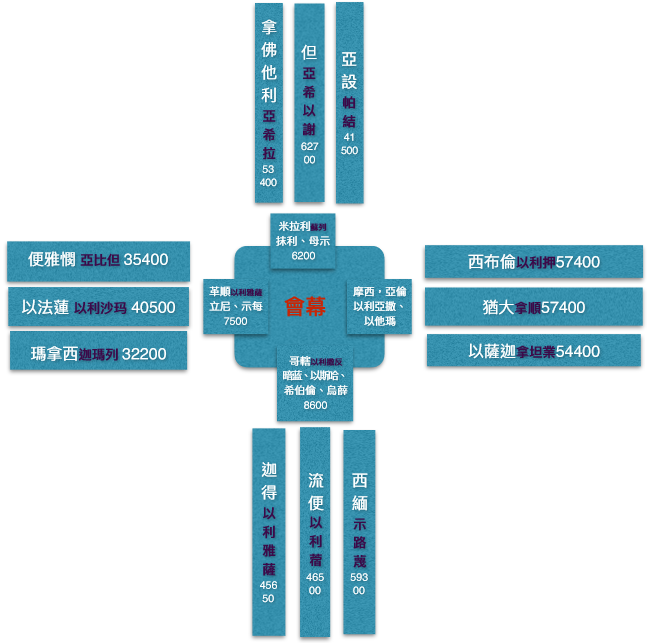
\includegraphics[width=0.85\textwidth]{AMoXiFigs/fig1}
\caption{各支派族長，人數及位置}
\label{fig:1} 
\end{center}
\end{wrapfigure}
耶和華曉諭摩西、亞倫說：「以色列人要各歸自己的纛下，在本族的旗號那裡，對著會幕的四圍安營。在\textcolor{red}{東邊}向日出之地，照著軍隊安營的是猶大營的纛。有亞米拿達的兒子拿順做猶大人的首領， 4 他軍隊被數的，共有七萬四千六百名； 5 挨著他安營的是以薩迦支派，有蘇押的兒子拿坦業做以薩迦人的首領， 6 他軍隊被數的，共有五萬四千四百名； 7 又有西布倫支派，希倫的兒子以利押做西布倫人的首領， 8 他軍隊被數的，共有五萬七千四百名。 9 凡屬猶大營，按著軍隊被數的，共有十八萬六千四百名，要做第一隊往前行。

\subsubsection{南邊支派首領及安營之所 2:9-16}
在\textcolor{red}{南邊}，按著軍隊是魯本營的纛。有示丟珥的兒子以利蓿做魯本人的首領， 11 他軍隊被數的，共有四萬六千五百名； 12 挨著他安營的是西緬支派，蘇利沙代的兒子示路蔑做西緬人的首領， 13 他軍隊被數的，共有五萬九千三百名； 14 又有迦得支派，丟珥的兒子以利雅薩做迦得人的首領， 15 他軍隊被數的，共有四萬五千六百五十名。 16 凡屬魯本營，按著軍隊被數的，共有十五萬一千四百五十名，要做第二隊往前行。

\subsubsection{利未營在諸營中間 2:17}
隨後會幕要往前行，有利未營在諸營\textcolor{red}{中間}。他們怎樣安營就怎樣往前行，各按本位，各歸本纛。

\subsubsection{西邊支派首領及安營之所 2:18-24}
在\textcolor{red}{西邊}，按著軍隊是以法蓮營的纛。亞米忽的兒子以利沙瑪做以法蓮人的首領， 19 他軍隊被數的，共有四萬零五百名； 20 挨著他的是瑪拿西支派，比大蓿的兒子迦瑪列做瑪拿西人的首領， 21 他軍隊被數的，共有三萬二千二百名； 22 又有便雅憫支派，基多尼的兒子亞比但做便雅憫人的首領， 23 他軍隊被數的，共有三萬五千四百名。 24 凡屬以法蓮營，按著軍隊被數的，共有十萬零八千一百名，要做第三隊往前行。

\subsubsection{北邊支派首領及安營之所 2:25-31}
在\textcolor{red}{北邊}，按著軍隊是但營的纛。亞米沙代的兒子亞希以謝做但人的首領， 26 他軍隊被數的，共有六萬二千七百名； 27 挨著他安營的是亞設支派，俄蘭的兒子帕結做亞設人的首領， 28 他軍隊被數的，共有四萬一千五百名； 29 又有拿弗他利支派，以南的兒子亞希拉做拿弗他利人的首領， 30 他軍隊被數的，共有五萬三千四百名。 31 凡但營被數的，共有十五萬七千六百名，要歸本纛做末隊往前行。

\subsection{數點利未支派 2:32－4:49}
\subsubsection{唯獨利未人沒有被數 2:32-34}
這些以色列人，照他們的宗族，按他們的軍隊，在諸營中被數的，共有六十萬零三千五百五十名。唯獨利未人沒有數在以色列人中，是照耶和華所吩咐摩西的。以色列人就這樣行，各人照他們的家室、宗族歸於本纛，安營起行，都是照耶和華所吩咐摩西的。

\subsubsection{亞倫和摩西的後代 3:1-4}
\begin{wraptable}{r}{5.cm}
\vspace*{-5mm}
\centering
\begin{tabular}{ c|c|c }\hline\hline
拿答-長子 & 獻凡火而死&受膏祭司\\ 
亞比戶 &獻凡火而死&受膏祭司\\  
以利亞撒 &供祭司職分&受膏祭司   \\
以他瑪  & 供祭司職分&受膏祭司   \\\hline
\end{tabular}
\caption{亞倫後裔}
\end{wraptable}
耶和華在西奈山曉諭摩西的日子，亞倫和摩西的後代如下：亞倫的兒子，長子名叫拿答，還有亞比戶、以利亞撒、以他瑪。這是亞倫兒子的名字，都是受膏的祭司，是摩西叫他們承接聖職供祭司職分的。拿答、亞比戶在西奈的曠野向耶和華獻凡火的時候，就死在耶和華面前了，他們也沒有兒子。以利亞撒、以他瑪在他們的父親亞倫面前供祭司的職分。

\subsubsection{區別利未人服侍亞倫 3:5-10}

耶和華曉諭摩西說：「你使利未支派近前來，站在祭司亞倫面前好服侍他，替他和會眾在會幕前守所吩咐的，辦理帳幕的事。又要看守會幕的器具，並守所吩咐以色列人的，辦理帳幕的事。你要將利未人給亞倫和他的兒子，因為他們是從以色列人中選出來給他的。你要囑咐亞倫和他的兒子謹守自己祭司的職任。近前來的外人必被治死。」

\subsubsection{利未人代替以色列人一切頭生 3:11-13}
耶和華曉諭摩西說： 12 「我從以色列人中揀選了利未人，代替以色列人一切頭生的，利未人要歸我， 13 因為凡頭生的是我的。我在埃及地擊殺一切頭生的那日，就把以色列中一切頭生的，連人帶牲畜都分別為聖歸我，他們定要屬我。我是耶和華。」

\subsubsection{利未宗族的家室 3:14-20}
\begin{figure}[H]
\centering
%\begin{center}
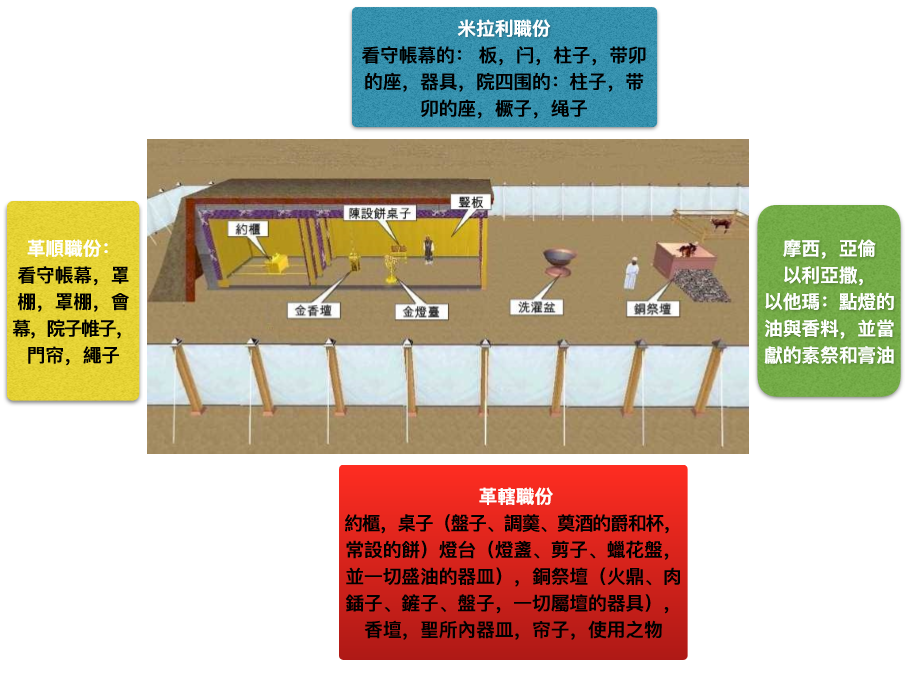
\includegraphics[width=5in]{AMoXiFigs/fig2}
\caption{圖2：利未各支派職分及位置}
\label{fig:1} 
%\end{center}
\end{figure}
耶和華在西奈的曠野曉諭摩西說： 15 「你要照利未人的宗族、家室數點他們，凡一個月以外的男子都要數點。」 16 於是摩西照耶和華所吩咐的，數點他們。 17 利未眾子的名字是革順、哥轄、米拉利。 18 革順的兒子，按著家室，是立尼、示每； 19 哥轄的兒子，按著家室，是暗蘭、以斯哈、希伯倫、烏薛； 20 米拉利的兒子，按著家室，是抹利、母示。這些按著宗族是利未人的家室。

\subsubsection{革順男丁之數及職份 3:21-26}
屬革順的，有立尼族、示每族，這是革順的二族。其中被數，從一個月以外所有的男子，共有七千五百名。這革順的二族要在帳幕後西邊安營。拉伊勒的兒子以利雅薩做革順人宗族的首領。革順的子孫在會幕中所要看守的，就是帳幕和罩篷，並罩篷的蓋與會幕的門簾，院子的帷子和門簾（院子是圍帳幕和壇的），並一切使用的繩子。

\subsubsection{革轄男丁之數及職份 3:27-43}
屬哥轄的，有暗蘭族、以斯哈族、希伯倫族、烏薛族，這是哥轄的諸族。按所有男子的數目，從一個月以外看守聖所的，共有八千六百名。哥轄兒子的諸族要在帳幕的南邊安營。烏薛的兒子以利撒反做哥轄宗族家室的首領。他們所要看守的是約櫃、桌子、燈臺、兩座壇與聖所內使用的器皿，並簾子和一切使用之物。祭司亞倫的兒子以利亞撒做利未人眾首領的領袖，要監察那些看守聖所的人。

\subsubsection{米拉利男丁之數及職份 3:33-37}
屬米拉利的，有瑪利族、母示族，這是米拉利的二族。他們被數的，按所有男子的數目，從一個月以外的，共有六千二百名。亞比亥的兒子蘇列做米拉利二宗族的首領。他們要在帳幕的北邊安營。米拉利子孫的職分是看守帳幕的板、閂、柱子、帶卯的座和帳幕一切所使用的器具，院子四圍的柱子、帶卯的座、橛子和繩子。

\subsubsection{摩西、亞倫和亞倫兒子的職份 3:38}
在帳幕前東邊向日出之地安營的是摩西、亞倫和亞倫的兒子。他們看守聖所，替以色列人守耶和華所吩咐的。近前來的外人必被治死。 

\subsubsection{利未人代替以色列族首生之男 3:39-51}
\begin{table}[H]
\centering
\begin{tabular}{c|c|c|c|c}
\hline
\hline
    &革順  & 革轄  & 米拉利&  總數  \\
\hline
各族     & 立尼，示每 & 暗蘭，以斯哈，希伯倫，烏薛  & 抹利，母示&   \\
\hline
人數（一個月以上）&7500&8600&6200&22000  \\ 
\hline
人數（30-50歲）& 2630 &  2750 &3200&8580  \\
\hline
\end{tabular}
\caption{利未支派}
\end{table}
39 凡被數的利未人，就是摩西、亞倫照耶和華吩咐所數的，按著家室，從一個月以外的男子，共有二萬二千名。

40 耶和華對摩西說：「你要從以色列人中數點一個月以外，凡頭生的男子，把他們的名字記下。 41 我是耶和華。你要揀選利未人歸我，代替以色列人所有頭生的；也取利未人的牲畜，代替以色列所有頭生的牲畜。」 42 摩西就照耶和華所吩咐的，把以色列人頭生的都數點了。 43 按人名的數目，從一個月以外，凡頭生的男子，共有二萬二千二百七十三名。

 耶和華曉諭摩西說：「你揀選利未人代替以色列人所有頭生的，也取利未人的牲畜代替以色列人的牲畜。利未人要歸我。我是耶和華。以色列人中頭生的男子比利未人多二百七十三個，必當將他們贖出來。你要按人丁，照聖所的平，每人取贖銀五舍客勒（一舍客勒是二十季拉），把那多餘之人的贖銀交給亞倫和他的兒子。」於是摩西從那被利未人所贖以外的人取了贖銀。從以色列人頭生的所取之銀，按聖所的平，有一千三百六十五舍客勒。摩西照耶和華的話把這贖銀給亞倫和他的兒子，正如耶和華所吩咐的。

\subsubsection{祭司亞倫和兒子職任 4:1-14}
耶和華曉諭摩西、亞倫說：「你從利未人中，將哥轄子孫的總數，照他們的家室、宗族，從三十歲直到五十歲，凡前來任職，在會幕裡辦事的，全都計算。哥轄子孫在會幕搬運至聖之物，所辦的事乃是這樣：起營的時候，亞倫和他兒子要進去
\begin{itemize} 
\itemsep-.35em
\item 摘下遮掩櫃的幔子，用以蒙蓋\textcolor{blue}{法櫃}。又用海狗皮蓋在上頭，再蒙上純藍色的毯子，把\textcolor{red}{槓}穿上。
\item 又用藍色毯子鋪在\textcolor{blue}{陳設餅的桌子上}，將盤子、調羹、奠酒的爵和杯擺在上頭，桌子上也必有常設的餅。在其上又要蒙朱紅色的毯子，再蒙上海狗皮，把\textcolor{red}{槓}穿上。
\item 要拿藍色毯子，把\textcolor{blue}{燈臺和燈臺上所用的}燈盞、剪子、蠟花盤並一切盛油的器皿，全都遮蓋。又要把燈臺和燈臺的一切器具包在海狗皮裡，放在\textcolor{red}{抬架}上。
\item 在\textcolor{blue}{金壇}上要鋪藍色毯子，蒙上海狗皮，把\textcolor{red}{槓}穿上。
\item 又要把聖所用的\textcolor{blue}{一切器具}包在藍色毯子裡，用海狗皮蒙上，放在\textcolor{red}{抬架}上。
\item 要收去壇上的灰，把紫色毯子鋪在壇上。又要把所用的一切器具，就是火鼎、肉叉子、鏟子、盤子，一切\textcolor{blue}{屬壇的器具}都擺在壇上。又蒙上海狗皮，把\textcolor{red}{槓}穿上。 
\end{itemize}

\subsubsection{哥轄子孫之職任 4:15-20}
將要起營的時候，\textcolor{blue}{亞倫和他兒子}把聖所和聖所的一切器具遮蓋完了，\textcolor{blue}{哥轄的子孫}就要來抬，只是不可摸聖物，免得他們死亡。會幕裡這些物件是哥轄子孫所當抬的。\textcolor{blue}{祭司亞倫的兒子以利亞撒}所要看守的是點燈的油與香料，並當獻的素祭和膏油，也要看守全帳幕與其中所有的，並聖所和聖所的器具。
耶和華曉諭摩西、亞倫說：「你們不可將哥轄人的支派從利未人中剪除。他們挨近至聖物的時候，\textcolor{blue}{亞倫和他兒子}要進去，派他們各人所當辦的、所當抬的。這樣待他們，好使他們活著，不致死亡。只是他們連片時不可進去觀看聖所，免得他們死亡。」

\subsubsection{革順子孫在以他瑪手下之職任 4:21-28}
耶和華曉諭摩西說：「你要將革順子孫的總數，照著宗族、家室，從三十歲直到五十歲，凡前來任職，在會幕裡辦事的，全都數點。革順人各族所辦的事、所抬的物乃是這樣：他們要抬帳幕的\textcolor{blue}{幔子}和會幕，並會幕的\textcolor{blue}{蓋}與其上的\textcolor{blue}{海狗皮}和會幕的\textcolor{blue}{門簾}，院子的\textcolor{blue}{帷子}和\textcolor{blue}{門簾}（院子是圍帳幕和壇的）、\textcolor{blue}{繩子}，並所用的\textcolor{blue}{器具}，不論是做什麼用的，他們都要經理。革順的子孫在一切抬物辦事之上都要憑亞倫和他兒子的吩咐。他們所當抬的，要派他們看守。這是革順子孫的各族在會幕裡所辦的事。他們所看守的，必在祭司亞倫兒子以他瑪的手下。

\subsubsection{米拉利子孫在以他瑪手下之職任 4:29-33}
至於米拉利的子孫，你要照著家室、宗族把他們數點。從三十歲直到五十歲，凡前來任職，在會幕裡辦事的，你都要數點。他們辦理會幕的事，就是抬帳幕的\textcolor{blue}{板、閂、柱子和帶卯的座}，院子四圍的\textcolor{blue}{柱子}和其上\textcolor{blue}{帶卯的座}，\textcolor{blue}{橛子}、\textcolor{blue}{繩子}，並\textcolor{blue}{一切使用的器具}。他們所抬的器具，你們要按名指定。這是米拉利子孫各族在會幕裡所辦的事，都在祭司亞倫兒子以他瑪的手下。

\subsubsection{記利未人自三十歲至五十歲者之數 4:34-49}
摩西、亞倫與會眾的諸首領將\textcolor{blue}{哥轄的子孫}，照著家室、宗族，從三十歲直到五十歲，凡前來任職，在會幕裡辦事的，都數點了，被數的共有二千七百五十名。這是哥轄各族中被數的，是在會幕裡辦事的，就是摩西、亞倫照耶和華藉摩西所吩咐數點的。
\textcolor{blue}{革順子孫}被數的，照著家室、宗族，從三十歲直到五十歲，凡前來任職，在會幕裡辦事的，共有二千六百三十名。這是革順子孫各族中被數的，是在會幕裡辦事的，就是摩西、亞倫照耶和華藉摩西所吩咐數點的。
\textcolor{blue}{米拉利子孫}中各族被數的，照著家室、宗族， 從三十歲直到五十歲，凡前來任職，在會幕裡辦事的，共有三千二百名。 這是米拉利子孫各族中被數的，就是摩西、亞倫照耶和華藉摩西所吩咐數點的。
凡\textcolor{blue}{被數的利未人}，就是摩西、亞倫並以色列眾首領，照著家室、宗族所數點的，從三十歲直到五十歲，凡前來任職，在會幕裡做抬物之工的，共有八千五百八十名。摩西按他們所辦的事、所抬的物，憑耶和華的吩咐數點他們。他們這樣被摩西數點，正如耶和華所吩咐他的。


\subsection{頒布生活，婚姻，生命潔净的律法 5-6}
\subsubsection{不潔者出到營外 5:1-4 }
耶和華曉諭摩西說：「你吩咐以色列人，使一切長大痲瘋的、患漏症的並因死屍不潔淨的，都出營外去。無論男女都要使他們出到營外，免得汙穢他們的營。這營是我所住的。」以色列人就這樣行，使他們出到營外。耶和華怎樣吩咐摩西，以色列人就怎樣行了。

\subsubsection{犯罪的要賠償 5:5-8}
耶和華對摩西說：「你曉諭以色列人說：無論男女，若犯了人所常犯的罪，以致干犯耶和華，那人就有了罪。他要承認所犯的罪，將所虧負人的如數賠還，另外加上五分之一，也歸於所虧負的人。那人若沒有親屬可受所賠還的，那所賠還的就要歸於服侍耶和華的祭司。至於那為他贖罪的公羊是在外。以色列人一切的聖物中，所奉給祭司的舉祭都要歸於祭司。各人所分別為聖的物，無論是什麼，都要歸給祭司。」

\subsubsection{歸給祭司的物 5:9-10}
以色列人一切的聖物中，所奉給祭司的舉祭都要歸於祭司。各人所分別為聖的物，無論是什麼，都要歸給祭司。

\subsubsection{妻子貞節實驗方法 5:11-31}
耶和華對摩西說： 12 「你曉諭以色列人說：人的妻若有邪行，得罪她丈夫， 13 有人與她行淫，事情嚴密，瞞過她丈夫，而且她被玷汙，沒有做見證的人，當她行淫的時候也沒有被捉住， 14 她丈夫生了疑恨的心，疑恨她，她是被玷汙，或是她丈夫生了疑恨的心，疑恨她，她並沒有被玷汙， 15 這人就要將妻送到祭司那裡，又為她帶著大麥麵伊法十分之一做供物，不可澆上油，也不可加上乳香，因為這是疑恨的素祭，是思念的素祭，使人思念罪孽。

祭司要使那婦人近前來，站在耶和華面前。 17 祭司要把聖水盛在瓦器裡，又從帳幕的地上取點塵土，放在水中。 18 祭司要叫那婦人蓬頭散髮，站在耶和華面前，把思念的素祭，就是疑恨的素祭，放在她手中。祭司手裡拿著致咒詛的苦水， 19 要叫婦人起誓，對她說：『若沒有人與你行淫，也未曾背著丈夫做汙穢的事，你就免受這致咒詛苦水的災。 20 你若背著丈夫行了汙穢的事，在你丈夫以外有人與你行淫， 21 （祭司叫婦人發咒起誓）願耶和華叫你大腿消瘦，肚腹發脹，使你在你民中被人咒詛，成了誓語， 22 並且這致咒詛的水入你的腸中，要叫你的肚腹發脹，大腿消瘦。』婦人要回答說：『阿們！阿們！』

祭司要寫這咒詛的話，將所寫的字抹在苦水裡， 24 又叫婦人喝這致咒詛的苦水。這水要進入她裡面變苦了。 25 祭司要從婦人的手中取那疑恨的素祭，在耶和華面前搖一搖，拿到壇前。 26 又要從素祭中取出一把，作為這事的紀念，燒在壇上，然後叫婦人喝這水。 27 叫她喝了以後，她若被玷汙，得罪了丈夫，這致咒詛的水必進入她裡面變苦了，她的肚腹就要發脹，大腿就要消瘦，那婦人便要在她民中被人咒詛； 28 若婦人沒有被玷汙，卻是清潔的，就要免受這災，且要懷孕。

妻子背著丈夫行了汙穢的事， 30 或是人生了疑恨的心，疑恨他的妻，就有這疑恨的條例。那時他要叫婦人站在耶和華面前，祭司要在她身上照這條例而行。 31 男人就為無罪，婦人必擔當自己的罪孽。

\noindent
疑恨（思念）的素祭=大麥麵1/10伊法+無油無乳香\\
1） 過程\\
  祭司要使那婦人近前來，站在耶和華面前發咒起誓；
  婦人要回答說：『阿們，阿們。』
  祭司要寫這咒詛的話，將所寫的字抹在苦水裏，從素祭中取出一把燒在壇上，叫婦人喝這水\\
2）判斷方法 \\
   $\cdot${ 她若被玷污得罪了丈夫，這致咒詛的水必進入她裏面變變苦了，她的肚腹就要發脹，大腿就要消瘦，那婦人便要在他民中被人咒詛。}\\
   $\cdot${ 若婦人沒有被玷污，卻是清潔的，就要免受這災，且要懷孕。}


\subsubsection{拿細耳人的條例 6:1-21}
\subsubsubsection{做拿細耳(歸主)人的要求 6:1-8}
耶和華對摩西說：「你曉諭以色列人說：無論男女許了特別的願，就是拿細耳(歸主)人的願，要離俗歸耶和華，
\vspace*{-2mm}
\begin{itemize} 
\itemsep-.35em
\item 他就要遠離清酒濃酒，也不可喝什麼清酒濃酒做的醋。不可喝什麼葡萄汁，也不可吃鮮葡萄和乾葡萄。在一切離俗的日子，凡葡萄樹上結的，自核至皮所做的物，都不可吃。
\item 在他一切許願離俗的日子，不可用剃頭刀剃頭，要由髮綹長長了。他要聖潔，直到離俗歸耶和華的日子滿了。
\item 在他離俗歸耶和華的一切日子，不可挨近死屍。他的父母或是弟兄姐妹死了的時候，他不可因他們使自己不潔淨，因為那離俗歸神的憑據是在他頭上。在他一切離俗的日子，是歸耶和華為聖。
\end{itemize} 

\subsubsubsection{拿細耳(歸主)人被沾染的要求 6:9-12}
\begin{itemize} 
\itemsep-.35em
\item 若在他旁邊忽然有人死了，以致沾染了他離俗的頭，他要在第七日得潔淨的時候剃頭。第八日，他要把兩隻斑鳩或兩隻雛鴿帶到會幕門口，交給祭司。
\item 祭司要獻一隻做贖罪祭，一隻做燔祭，為他贖那因死屍而有的罪，並要當日使他的頭成為聖潔。
\item 他要另選離俗歸耶和華的日子，又要牽一隻一歲的公羊羔來做贖愆祭；但先前的日子要歸徒然，因為他在離俗之間被玷汙了。
\end{itemize} 

\subsubsubsection{拿細耳(歸主)滿了離俗期的條例 6:13-21}
拿細耳人滿了離俗的日子乃有這條例：
\vspace*{-2mm}
\begin{itemize} 
\itemsep-.35em
\item 人要領他到會幕門口，他要將供物奉給耶和華，就是一隻沒有殘疾、一歲的公羊羔做燔祭，一隻沒有殘疾、一歲的母羊羔做贖罪祭，和一隻沒有殘疾的公綿羊做平安祭，並一筐子無酵調油的細麵餅與抹油的無酵薄餅，並同獻的素祭和奠祭。
\item 祭司要在耶和華面前獻那人的贖罪祭和燔祭，也要把那隻公羊和那筐無酵餅獻給耶和華做平安祭，又要將同獻的素祭和奠祭獻上。
\item 拿細耳人要在會幕門口剃離俗的頭，把離俗頭上的髮放在平安祭下的火上。
\item 他剃了以後，祭司就要取那已煮的公羊一條前腿，又從筐子裡取一個無酵餅和一個無酵薄餅，都放在他手上。祭司要拿這些作為搖祭，在耶和華面前搖一搖，這與所搖的胸、所舉的腿同為聖物，歸給祭司。
\item 然後，拿細耳人可以喝酒。
\end{itemize}
\vspace*{-2mm}
許願的拿細耳人為離俗所獻的供物和他以外所能得的獻給耶和華，就有這條例。他怎樣許願就當照離俗的條例行。

\subsubsection{祭司為以色列人祝福之語 6:22-27}
耶和華曉諭摩西說：「你告訴亞倫和他兒子說，你們要這樣為以色列人祝福，說：
\vspace*{-2mm}
\begin{itemize} 
\itemsep-.35em
\item \textcolor{blue}{願耶和華}賜福給你，保護你！
\item \textcolor{blue}{願耶和華}使他的臉光照你，賜恩給你！
\item \textcolor{blue}{願耶和華}向你仰臉，賜你平安！
\end{itemize} 
\vspace*{-2mm}
他們要如此奉我的名為以色列人祝福，我也要賜福給他們。」


%\subsection{信仰分别为聖各族長向會幕獻祭 7}
\subsection{信仰分别為聖-各族長向會幕獻祭 7:1-89}
\subsubsection{會幕建立族長獻禮 7:1-3}
摩西立完了帳幕，就\textcolor{blue}{把帳幕用膏抹}了，使它\textcolor{red}{成聖}；又把其中的\textcolor{blue}{器具和壇並壇上的器具，都抹}了，使它\textcolor{red}{成聖}。\textcolor{red}{當天}，以色列的眾首領，就是\textcolor{blue}{各族的族長}，都來奉獻。他們是各支派的首領管理那些被數的人。他們把自己的供物送到耶和華面前，就是六輛篷子車和十二隻公牛。每兩個首領奉獻一輛車，每首領奉獻一隻牛。他們把這些都\textcolor{blue}{奉到帳幕前}。

\subsubsection{族長獻禮的分配原则 7:4-10}
\begin{wraptable}{r}{5.cm}
%\vspace*{-5mm}
\centering
\begin{tabular}{|c|c|c|c|}
\hline
\hline
     &革轄 &革順  & 米拉利    \\
\hline
車子 & -   & 兩輛&四輛   \\
\hline
公牛&- &四隻&八隻  \\ 
\hline
\end{tabular}
\caption{眾族長獻禮的分配}
\end{wraptable}
%\vspace*{-4mm}
耶和華曉諭摩西說：「你要收下這些，好做會幕的使用，都要照利未人所辦的事交給他們。」於是摩西收了車和牛，交給利未人，把兩輛車、四隻牛，照\textcolor{blue}{革順子孫}所辦的事交給他們，又把四輛車、八隻牛，照\textcolor{blue}{米拉利子孫}所辦的事交給他們。他們都在祭司亞倫的兒子以他瑪手下。但車與牛都\textcolor{blue}{沒有交給哥轄子孫}，因為他們辦的是聖所的事，在肩頭上抬聖物。用\textcolor{blue}{膏抹壇的日子}，首領都來行奉獻壇的禮，眾首領就在\textcolor{blue}{壇前獻供物}。

\subsubsection{眾族長獻供物及獻禮顺序 7:11-83}

\begin{table}[H]
\centering
\begin{tabular}{|c|c|c|c|c|}
\hline
\hline
 素祭 & 香 & 燔祭 & 贖罪祭 & 平安祭 \\\hline
銀盤子（130舍客勒）&金盂& 公牛（1）&公山羊(1) &公牛（2） \\
銀碗（70舍客勒）     &（10舍客勒）& 公綿羊(1)         &           & 公綿羊（5）/ 公山羊（5）  \\
盛滿調油細麵         &盛滿了香   & 一歲的公羊羔(1) &          &一歲的公羊羔（5）   \\\hline
\end{tabular}
\caption{各首領向會幕獻的祭物}
\end{table}

\begin{table}[H]
\centering
\begin{tabular}{|c|c|c|c|c|}
\hline
\hline
營纛  & 獻祭次序&  支派 &首領名字 &父親名字 \\
\hline
\multirow{3}{*}{猶大營} & 第一日    & \textcolor{red}{猶大} &拿順 &亞米拿達  \\
\cline{2-5}
\multicolumn{1}{|c|}{}  & 第二日  & 以薩迦 &拿坦業  & 蘇押  \\
\cline{2-5}
\multicolumn{1}{|c|}{} & 第三日  & 西布倫&  以利押& 希倫  \\
\cline{2-5}
\hline
\multirow{3}{*}{流便營} &  第四日  &\textcolor{red}{流便}  &以利蓿 & 示丟珥 \\
\cline{2-5}
\multicolumn{1}{|c|}{}  &   第五日 &西緬  & 示路蔑 &  蘇利沙代  \\
\cline{2-5}
\multicolumn{1}{|c|}{} & 第六日  & 迦得&以利雅薩 & 丟珥  \\
\hline
\multirow{3}{*}{以法蓮營} &  第七日  &\textcolor{red}{以法蓮}  &以利沙瑪 & 亞米忽 \\
\cline{2-5}
\multicolumn{1}{|c|}{}  &   第八日 &瑪拿西  & 迦瑪列 &  比大蓿  \\
\cline{2-5}
\multicolumn{1}{|c|}{} & 第九日  & 便雅憫&亞比但 & 基多尼  \\
\hline
\multirow{3}{*}{但營} &  第十日  &\textcolor{red}{但}  &亞希以謝 & 亞米沙代 \\
\cline{2-5}
\multicolumn{1}{|c|}{}  &   第十一日 &亞設  & 帕結 &  俄蘭  \\
\cline{2-5}
\multicolumn{1}{|c|}{} & 第十二日  & 拿弗他利&亞希拉 & 以南  \\
\hline
\end{tabular}
\caption{各族長獻祭次序}
\end{table}


\subsubsubsection{頭一日猶大支派獻禮 7:11-17}
耶和華對摩西說：「眾首領為行奉獻壇的禮，要每天一個首領來獻供物。」頭一日獻供物的是猶大支派的亞米拿達的兒子拿順。他的供物是：一個銀盤子，重一百三十舍客勒，一個銀碗，重七十舍客勒，都是按聖所的平，也都盛滿了調油的細麵做素祭。一個金盂，重十舍客勒，盛滿了香。一隻公牛犢，一隻公綿羊，一隻一歲的公羊羔做燔祭；一隻公山羊做贖罪祭；兩隻公牛，五隻公綿羊，五隻公山羊，五隻一歲的公羊羔做平安祭。這是亞米拿達兒子拿順的供物。

\subsubsubsection{第二日以薩迦支派獻禮 7:18-23}
第二日來獻的是以薩迦子孫的首領，蘇押的兒子拿坦業。他獻為供物的是：一個銀盤子，重一百三十舍客勒，一個銀碗，重七十舍客勒，都是按聖所的平，也都盛滿了調油的細麵做素祭。一個金盂，重十舍客勒，盛滿了香。一隻公牛犢，一隻公綿羊，一隻一歲的公羊羔做燔祭；一隻公山羊做贖罪祭；兩隻公牛，五隻公綿羊，五隻公山羊，五隻一歲的公羊羔做平安祭。這是蘇押兒子拿坦業的供物。

\subsubsubsection{第三日西布倫支派獻禮 7:24-29}
第三日來獻的是西布倫子孫的首領，希倫的兒子以利押。他的供物是：一個銀盤子，重一百三十舍客勒，一個銀碗，重七十舍客勒，都是按聖所的平，也都盛滿了調油的細麵做素祭。一個金盂，重十舍客勒，盛滿了香。 一隻公牛犢，一隻公綿羊，一隻一歲的公羊羔做燔祭； 一隻公山羊做贖罪祭；兩隻公牛，五隻公綿羊，五隻公山羊，五隻一歲的公羊羔做平安祭。這是希倫兒子以利押的供物。

\subsubsubsection{第四日魯本支派獻禮 7:30-35}
第四日來獻的是魯本子孫的首領，示丟珥的兒子以利蓿。他的供物是：一個銀盤子，重一百三十舍客勒，一個銀碗，重七十舍客勒，都是按聖所的平，也都盛滿了調油的細麵做素祭。一個金盂，重十舍客勒，盛滿了香。一隻公牛犢，一隻公綿羊，一隻一歲的公羊羔做燔祭；一隻公山羊做贖罪祭；兩隻公牛，五隻公綿羊，五隻公山羊，五隻一歲的公羊羔做平安祭。這是示丟珥的兒子以利蓿的供物。

\subsubsubsection{第五日西緬支派獻禮 7:36-41}
第五日來獻的是西緬子孫的首領，蘇利沙代的兒子示路蔑。他的供物是：一個銀盤子，重一百三十舍客勒，一個銀碗，重七十舍客勒，都是按聖所的平，也都盛滿了調油的細麵做素祭。一個金盂，重十舍客勒，盛滿了香。一隻公牛犢，一隻公綿羊，一隻一歲的公羊羔做燔祭；一隻公山羊做贖罪祭；兩隻公牛，五隻公綿羊，五隻公山羊，五隻一歲的公羊羔做平安祭。這是蘇利沙代兒子示路蔑的供物。


\subsubsubsection{第六日迦得支派獻禮 7:42-47}
第六日來獻的是迦得子孫的首領，丟珥的兒子以利雅薩他的供物是：一個銀盤子，重一百三十舍客勒，一個銀碗，重七十舍客勒，都是按聖所的平，也都盛滿了調油的細麵做素祭。一個金盂，重十舍客勒，盛滿了香。一隻公牛犢，一隻公綿羊，一隻一歲的公羊羔做燔祭；一隻公山羊做贖罪祭；兩隻公牛，五隻公綿羊，五隻公山羊，五隻一歲的公羊羔做平安祭。這是丟珥的兒子以利雅薩的供物。

\subsubsubsection{第七日以法蓮支派獻禮 7:48-53}
第七日來獻的是以法蓮子孫的首領，亞米忽的兒子以利沙瑪。他的供物是：一個銀盤子，重一百三十舍客勒，一個銀碗，重七十舍客勒，都是按聖所的平，也都盛滿了調油的細麵做素祭。一個金盂，重十舍客勒，盛滿了香。一隻公牛犢，一隻公綿羊，一隻一歲的公羊羔做燔祭；一隻公山羊做贖罪祭；兩隻公牛，五隻公綿羊，五隻公山羊，五隻一歲的公羊羔做平安祭。這是亞米忽兒子以利沙瑪的供物。

\subsubsubsection{第八日瑪拿西支派獻禮 7:54-59}
第八日來獻的是瑪拿西子孫的首領，比大蓿的兒子迦瑪列。他的供物是：一個銀盤子，重一百三十舍客勒，一個銀碗，重七十舍客勒，都是按聖所的平，也都盛滿了調油的細麵做素祭。一個金盂，重十舍客勒，盛滿了香。一隻公牛犢，一隻公綿羊，一隻一歲的公羊羔做燔祭；一隻公山羊做贖罪祭； 兩隻公牛，五隻公綿羊，五隻公山羊，五隻一歲的公羊羔做平安祭。這是比大蓿兒子迦瑪列的供物。

\subsubsubsection{第九日便雅憫支派獻禮 7:60-65}
第九日來獻的是便雅憫子孫的首領，基多尼的兒子亞比但。他的供物是：一個銀盤子，重一百三十舍客勒，一個銀碗，重七十舍客勒，都是按聖所的平，也都盛滿了調油的細麵做素祭。一個金盂，重十舍客勒，盛滿了香。一隻公牛犢，一隻公綿羊，一隻一歲的公羊羔做燔祭；一隻公山羊做贖罪祭；兩隻公牛，五隻公綿羊，五隻公山羊，五隻一歲的公羊羔做平安祭。這是基多尼兒子亞比但的供物。

\subsubsubsection{第十日但支派獻禮 7:66-71}
第十日來獻的是但子孫的首領，亞米沙代的兒子亞希以謝。他的供物是：一個銀盤子，重一百三十舍客勒，一個銀碗，重七十舍客勒，都是按聖所的平，也都盛滿了調油的細麵做素祭。一個金盂，重十舍客勒，盛滿了香。一隻公牛犢，一隻公綿羊，一隻一歲的公羊羔做燔祭；一隻公山羊做贖罪祭；兩隻公牛，五隻公綿羊，五隻公山羊，五隻一歲的公羊羔做平安祭。這是亞米沙代兒子亞希以謝的供物。

\subsubsubsection{第十一日西布倫支派獻禮 7:72-77}
第十一日來獻的是亞設子孫的首領，俄蘭的兒子帕結。他的供物是：一個銀盤子，重一百三十舍客勒，一個銀碗，重七十舍客勒，都是按聖所的平，也都盛滿了調油的細麵做素祭。一個金盂，重十舍客勒，盛滿了香。一隻公牛犢，一隻公綿羊，一隻一歲的公羊羔做燔祭； 一隻公山羊做贖罪祭；兩隻公牛，五隻公綿羊，五隻公山羊，五隻一歲的公羊羔做平安祭。這是俄蘭兒子帕結的供物。

\subsubsubsection{第十二日拿弗他利支派獻禮 7:78-83}
第十二日來獻的是拿弗他利子孫的首領，以南兒子亞希拉。他的供物是：一個銀盤子，重一百三十舍客勒，一個銀碗，重七十舍客勒，都是按聖所的平，也都盛滿了調油的細麵做素祭。一個金盂，重十舍客勒，盛滿了香。一隻公牛犢，一隻公綿羊，一隻一歲的公羊羔做燔祭；一隻公山羊做贖罪祭；兩隻公牛，五隻公綿羊，五隻公山羊，五隻一歲的公羊羔做平安祭。這是以南兒子亞希拉的供物。

\subsubsection{眾首領為行獻壇之禮所獻禮物 7:84-88}
用膏抹壇的日子，以色列的眾首領為行獻壇之禮所獻的是：銀盤子十二個，銀碗十二個，金盂十二個。每盤子重一百三十舍客勒，每碗重七十舍客勒。一切器皿的銀子，按聖所的平，共有二千四百舍客勒。十二個金盂盛滿了香，按聖所的平，每盂重十舍客勒，所有的金子共一百二十舍客勒。做燔祭的，共有公牛十二隻，公羊十二隻，一歲的公羊羔十二隻；並同獻的素祭；做贖罪祭的公山羊十二隻；做平安祭的，共有公牛二十四隻，公綿羊六十隻，公山羊六十隻，一歲的公羊羔六十隻。這就是用膏抹壇之後，為行奉獻壇之禮所獻的。

\subsubsection{耶和華在施恩座以上與摩西說話 7:89}
摩西進會幕要與耶和華說話的時候，聽見法櫃的施恩座以上，二基路伯中間有與他說話的聲音，就是耶和華與他說話。

\subsection{信仰分别為聖-利未人的條例 8:1-9:14}
\subsubsection{點燈的條例 8:1-4 }
耶和華曉諭摩西說：「你告訴亞倫說：點燈的時候，七盞燈都要向燈臺前面發光。」 3 亞倫便這樣行。他點燈臺上的燈，使燈向前發光，是照耶和華所吩咐摩西的。 4 這燈臺的做法是用金子錘出來的，連座帶花都是錘出來的。摩西製造燈臺，是照耶和華所指示的樣式。

\subsubsection{潔淨利未人的條例 8:5-7}
\noindent
耶和華曉諭摩西說：你從以色列人中選出利未人來，潔淨他們。潔淨他們當這樣行：用除罪水彈在他們身上，又叫他們用剃頭刀刮全身，洗衣服，潔淨自己。
 
\subsubsection{為利未人獻祭的條例 8:5-12}
然後叫他們取一隻公牛犢，並同獻的素祭，就是調油的細麵。你要另取一隻公牛犢做贖罪祭。 9 將利未人奉到會幕前，招聚以色列全會眾。 10 將利未人奉到耶和華面前，以色列人要按手在他們頭上。 11 亞倫也將他們奉到耶和華面前，為以色列人當做搖祭，使他們好辦耶和華的事。 12 利未人要按手在那兩隻牛的頭上，你要將一隻做贖罪祭，一隻做燔祭，獻給耶和華，為利未人贖罪。

\subsubsection{利未人做搖祭代替以色列頭生 8:13-19}
你也要使利未人站在亞倫和他兒子面前，將他們當做搖祭奉給耶和華。這樣，你從以色列人中將利未人分別出來，利未人便要歸我。此後利未人要進去辦會幕的事，你要潔淨他們，將他們當做搖祭奉上。因為他們是從以色列人中全然給我的，我揀選他們歸我，是代替以色列人中一切頭生的。以色列人中一切頭生的，連人帶牲畜，都是我的，我在埃及地擊殺一切頭生的那天，將他們分別為聖歸我。我揀選利未人代替以色列人中一切頭生的。我從以色列人中將利未人當做賞賜給亞倫和他的兒子，在會幕中辦以色列人的事，又為以色列人贖罪，免得他們挨近聖所，有災殃臨到他們中間。」

\subsubsection{摩西、亞倫並以色列全會眾照此向利未人行 8:20-22}
\textcolor{blue}{摩西、亞倫並以色列全會眾}便向利未人如此行。凡耶和華指著利未人所吩咐摩西的，以色列人就向他們這樣行。於是\textcolor{blue}{利未人}潔淨自己，除了罪，洗了衣服。\textcolor{blue}{亞倫}將他們當做搖祭奉到耶和華面前，又為他們贖罪，潔淨他們。然後利未人進去，在亞倫和他兒子面前，在會幕中辦事。耶和華指著利未人怎樣吩咐摩西，以色列人就怎樣向他們行了。

\subsubsection{利未人任職的要求 8:23-26}
耶和華曉諭摩西說：「利未人是這樣：從\textcolor{blue}{二十五歲以外}，他們要前來任職，辦會幕的事。到了\textcolor{blue}{五十歲要停工退任}，不再辦事，只要在會幕裡，和他們的弟兄一同伺候，謹守所吩咐的，不再辦事了。至於所吩咐利未人的，你要這樣向他們行。」


\subsubsection{正月十四日守逾越節 9:1-5}
\noindent
以色列人出埃及地以後，第二年正月，耶和華在西奈的曠野吩咐摩西說： 2 「以色列人應當在所定的日期守逾越節， 3 就是本月十四日黃昏的時候，你們要在所定的日期守這節，要按這節的律例、典章而守。」 4 於是摩西吩咐以色列人守逾越節。 5 他們就在西奈的曠野，正月十四日黃昏的時候，守逾越節。凡耶和華所吩咐摩西的，以色列人都照樣行了。
 
\subsubsection{二月十四日补守逾越節的條例  9:6-14 }
有幾個人因死屍而不潔淨，不能在那日守逾越節。當日他們到摩西、亞倫面前， 7 說：「我們雖因死屍而不潔淨，為何被阻止，不得同以色列人在所定的日期獻耶和華的供物呢？」 8 摩西對他們說：「你們暫且等候，我可以去聽耶和華指著你們是怎樣吩咐的。」

耶和華對摩西說：「你曉諭以色列人說：你們和你們後代中，若有人因死屍而不潔淨，或在遠方行路，還要向耶和華守逾越節。他們要在二月十四日黃昏的時候守逾越節，要用無酵餅與苦菜和逾越節的羊羔同吃。一點不可留到早晨，羊羔的骨頭一根也不可折斷。他們要照逾越節的一切律例而守。那潔淨而不行路的人若推辭不守逾越節，那人要從民中剪除，因為他在所定的日期不獻耶和華的供物，應該擔當他的罪。 14 若有外人寄居在你們中間，願意向耶和華守逾越節，他要照逾越節的律例、典章行，不管是寄居的，是本地人，同歸一例。」

\subsection{起行安營 9:15-9:36}
\subsubsection{起行安營的條例 9:15-23}
\noindent
立起帳幕的那日，有雲彩遮蓋帳幕，就是法櫃的帳幕。從晚上到早晨，雲彩在其上，形狀如火。常是這樣，雲彩遮蓋帳幕，夜間形狀如火。雲彩幾時從帳幕收上去，以色列人就幾時起行。雲彩在哪裡停住，以色列人就在哪裡安營。以色列人遵耶和華的吩咐起行，也遵耶和華的吩咐安營。雲彩在帳幕上停住幾時，他們就住營幾時。雲彩在帳幕上停留許多日子，以色列人就守耶和華所吩咐的不起行。有時雲彩在帳幕上幾天，他們就照耶和華的吩咐住營，也照耶和華的吩咐起行。有時從晚上到早晨有這雲彩在帳幕上，早晨雲彩收上去，他們就起行。有時晝夜雲彩停在帳幕上，收上去的時候，他們就起行。 雲彩停留在帳幕上，無論是兩天，是一月，是一年，以色列人就住營不起行，但雲彩收上去，他們就起行。他們遵耶和華的吩咐安營，也遵耶和華的吩咐起行。他們守耶和華所吩咐的，都是憑耶和華吩咐摩西的。

\subsubsection{吹號的條例 10:1-10}
\noindent
耶和華曉諭摩西說：你要用銀子做兩支號，都要錘出來的，用以招聚會眾，並叫眾營起行。吹這號的時候，全會眾要到你那裡，聚集在會幕門口。\\
1) 若單吹一支，眾首領，就是以色列軍中的統領，要聚集到你那裡。\\
2) 吹出大聲的時候，東邊安的營都要起行。二次吹出大聲的時候，南邊安的營都要起行。他們將起行，必吹出大聲。\\
3) 但招聚會眾的時候，你們要吹號，卻不要吹出大聲。\\
亞倫子孫做祭司的要吹這號，這要做你們世世代代永遠的定例。\\
4) 你們在自己的地與欺壓你們的敵人打仗，就要用號吹出大聲，便在耶和華你們的神面前得蒙記念，也蒙拯救脫離仇敵。\\
5) 在你們快樂的日子和節期並月朔獻燔祭和平安祭，也要吹號，這都要在你們的神面前作為紀念。我是耶和華你們的神。 

\subsubsection{起行的次序 10:11-27}
\noindent
\begin{wraptable}{r}{12cm}
\begin{tabular}{|c|c|c|c|c|c|}
\hline
\hline
第一隊  & 第二隊(利末人)&  第三隊 &第四隊(利末人) &第五隊&第六隊 \\\hline
猶大營 & 革順的子孫    &流便 &哥轄人 & 以法蓮& 但 \\
%\cline{2-5}
以薩迦  & 米拉利的子孫  & 西緬 &擡著聖物  & 瑪拿西& 亞設\\
%\cline{2-5}
西布倫 & 擡著帳幕先往前行  &迦得&   & 便雅憫& 拿弗他利 \\
%\cline{2-5}
%\hline
\hline
\end{tabular}
\caption{起行次序}
\end{wraptable}
\textcolor{blue}{第二年二月二十日}，雲彩從法櫃的帳幕收上去。以色列人就按站往前行，離開西乃的曠野，雲彩停住在巴蘭的曠野。這是他們\textcolor{blue}{初次往前行}。 \\
按著軍隊首先往前行的是\textcolor{red}{猶大營}的纛，統領軍隊的是亞米拿達的兒子拿順。統領以薩迦支派軍隊的是蘇押的兒子拿坦業。統領西布倫支派軍隊的是希倫的兒子以利押。帳幕拆卸，\textcolor{red}{革順的子孫和米拉利的子孫}就抬著帳幕先往前行。按著軍隊往前行的是\textcolor{red}{魯本營}的纛，統領軍隊的是示丟珥的兒子以利蓿。統領西緬支派軍隊的是蘇利沙代的兒子示路蔑。統領迦得支派軍隊的是丟珥的兒子以利雅薩。\textcolor{red}{哥轄人}抬著聖物先往前行，他們未到以前，抬帳幕的已經把帳幕支好。按著軍隊往前行的是\textcolor{red}{以法蓮營}的纛，統領軍隊的是亞米忽的兒子以利沙瑪。統領瑪拿西支派軍隊的是比大蓿的兒子迦瑪列。統領便雅憫支派軍隊的是基多尼的兒子亞比但。在\textcolor{red}{諸營末後的是但營}的纛，按著軍隊往前行，統領軍隊的是亞米沙代的兒子亞希以謝。統領亞設支派軍隊的是俄蘭的兒子帕結。統領拿弗他利支派軍隊的是以南的兒子亞希拉。以色列人按著軍隊往前行，就是這樣。

\subsubsection{摩西求岳父米甸人同行 10:28-32}
摩西對他岳父（內兄）米甸人流珥的兒子何巴說：「我們要行路，往耶和華所應許之地去。他曾說：『我要將這地賜給你們。』現在求你和我們同去，我們必厚待你，因為耶和華指著以色列人已經應許給好處。」 30 何巴回答說：「我不去，我要回本地本族那裡去。」 31 摩西說：「求你不要離開我們，因為你知道我們要在曠野安營，你可以當做我們的眼目。 32 你若和我們同去，將來耶和華有什麼好處待我們，我們也必以什麼好處待你。」

\subsubsection{以色列人離開耶和華的山 10:33-34}
\begin{figure}[H] 
\begin{center} 
\includegraphics[width=5.in]{AMoXiFigs/minshuji/fig3}
\caption{圖1：各支派族長，人數及位置}
\label{fig:1} 
\end{center}
\end{figure}
以色列人離開耶和華的山，往前行了三天的路程。耶和華的約櫃在前頭行了三天的路程，為他們尋找安歇的地方。他們拔營往前行，日間有耶和華的雲彩在他們以上。

\subsubsection{摩西在約櫃前行停住時候的祷告 10:35-36}
約櫃往前行的時候，摩西就說：「耶和華啊，求你興起！願你的仇敵四散，願恨你的人從你面前逃跑！」約櫃停住的時候，他就說：「耶和華啊，求你回到以色列的千萬人中！」


\section{从西乃至摩押平原 11-20}

\subsection{眾百姓的叛乱-他備拉發怨言 11:1-3}
%\subsubsection{他備拉眾百姓發怨言 11:1-3}
眾百姓發怨言，他們的惡語達到耶和華的耳中。耶和華聽見了就怒氣發作，使火在他們中間焚燒，直燒到營的邊界。百姓向摩西哀求，摩西祈求耶和華，火就熄了。那地方便叫做他備拉，因為耶和華的火燒在他們中間。


\subsection{眾百姓的叛乱-基博羅哈他瓦抱怨嗎哪的貪慾之人 11:4-34}
\subsubsection{以色列人因嗎哪单调發怨言 11:4-6}
他們中間的閒雜人大起貪慾的心。以色列人又哭號說：「誰給我們肉吃呢？我們記得在埃及的時候不花錢就吃魚，也記得有黃瓜、西瓜、韭菜、蔥、蒜。 現在我們的心血枯竭了，除這嗎哪以外，在我們眼前並沒有別的東西！」

\subsubsection{关于嗎哪 11:7-9}
這嗎哪彷彿芫荽子，又好像珍珠。百姓周圍行走，把嗎哪收起來，或用磨推，或用臼搗，煮在鍋中，又做成餅，滋味好像新油。夜間露水降在營中，嗎哪也隨著降下。

\subsubsection{摩西因管理百姓責任太重先神求死 11:10-15}
摩西聽見百姓各在各家的帳篷門口哭號。耶和華的怒氣便大發作，摩西就不喜悅。摩西對耶和華說：「你為何苦待僕人，我為何不在你眼前蒙恩，竟把這管理百姓的重任加在我身上呢？這百姓豈是我懷的胎，豈是我生下來的呢？你竟對我說把他們抱在懷裡，如養育之父抱吃奶的孩子，直抱到你起誓應許給他們祖宗的地去。我從哪裡得肉給這百姓吃呢？他們都向我哭號說：『你給我們肉吃吧！』管理這百姓的責任太重了，我獨自擔當不起。你這樣待我，我若在你眼前蒙恩，求你立時將我殺了，不叫我見自己的苦情。」

\subsubsection{招聚長老中七十人輔助摩西 11:16-17}
耶和華對摩西說：「你從以色列的長老中招聚七十個人，就是你所知道做百姓的長老和官長的，到我這裡來，領他們到會幕前，使他們和你一同站立。我要在那裡降臨，與你說話，也要把降於你身上的靈分賜他們，他們就和你同當這管百姓的重任，免得你獨自擔當。

\subsubsection{耶和華要百姓自潔預備明天吃肉 11:18-23}
又要對百姓說：你們應當自潔，預備明天吃肉，因為你們哭號說：『誰給我們肉吃？我們在埃及很好。』這聲音達到了耶和華的耳中，所以他必給你們肉吃。你們不止吃一天兩天，五天十天，二十天，要吃一個整月，甚至肉從你們鼻孔裡噴出來，使你們厭惡了，因為你們厭棄住在你們中間的耶和華，在他面前哭號說：『我們為何出了埃及呢？』」摩西對耶和華說：「這與我同住的百姓，步行的男人有六十萬，你還說『我要把肉給他們，使他們可以吃一個整月』？難道給他們宰了羊群牛群，或是把海中所有的魚都聚了來，就夠他們吃嗎？」耶和華對摩西說：「耶和華的膀臂豈是縮短了嗎？現在要看我的話向你應驗不應驗。」

\subsubsection{靈降在長老中七十人身上 11:24-25}
摩西出去，將耶和華的話告訴百姓，又招聚百姓的長老中七十個人來，使他們站在會幕的四圍。耶和華在雲中降臨，對摩西說話，把降於他身上的靈分賜那七十個長老。靈停在他們身上的時候，他們就受感說話，以後卻沒有再說。

\subsubsection{約書亞為靈降在營裡兩人身上而生嫉妒 11:26-30}
但有兩個人仍在營裡，一個名叫伊利達，一個名叫米達。他們本是在那些被錄的人中，卻沒有到會幕那裡去。靈停在他們身上，他們就在營裡說預言。有個少年人跑來告訴摩西說：「伊利達、米達在營裡說預言。」摩西的幫手，嫩的兒子約書亞，就是摩西所揀選的一個人，說：「請我主摩西禁止他們！」摩西對他說：「你為我的緣故嫉妒人嗎？唯願耶和華的百姓都受感說話，願耶和華把他的靈降在他們身上！」於是摩西和以色列的長老都回到營裡去。

\subsubsection{民貪食鵪鶉而遘重災 11:31-34}
有風從耶和華那裡颳起，把鵪鶉由海面颳來，飛散在營邊和營的四圍。這邊約有一天的路程，那邊約有一天的路程，離地面約有二肘。百姓起來，終日終夜，並次日一整天，捕取鵪鶉，至少的也取了十賀梅珥，為自己擺列在營的四圍。肉在他們牙齒之間尚未嚼爛，耶和華的怒氣就向他們發作，用最重的災殃擊殺了他們。那地方便叫做基博羅哈他瓦 （慾之人的墳墓），因為他們在那裡葬埋那起貪慾之心的人。 

\subsection{在哈洗錄毀謗摩西 11:35-12:15}
\subsubsection{米利暗和亞倫因古實女子毀謗摩西 11:35-12:3}
百姓從基博羅哈他瓦走到哈洗錄，就住在哈洗錄。摩西娶了古實女子為妻。米利暗和亞倫因他所娶的古實女子就毀謗他，說：「難道耶和華單與摩西說話，不也與我們說話嗎？」這話耶和華聽見了。摩西為人極其謙和，勝過世上的眾人。

\subsubsection{耶和華责备亞倫和米利暗 12:4-9}
耶和華忽然對摩西、亞倫、米利暗說：「你們三個人都出來，到會幕這裡。」他們三個人就出來了。耶和華在雲柱中降臨，站在會幕門口，召亞倫和米利暗，二人就出來了。耶和華說：「你們且聽我的話，你們中間若有先知，我耶和華必在異象中向他顯現，在夢中與他說話。我的僕人摩西不是這樣，他是在我全家盡忠的，我要與他面對面說話，乃是明說，不用謎語，並且他必見我的形象。你們毀謗我的僕人摩西，為何不懼怕呢？」耶和華就向他們二人發怒而去。

\subsubsection{米利暗長大痲瘋摩西哀求耶和華 12:10-12:15}
雲彩從會幕上挪開了，不料，米利暗長了大痲瘋，有雪那樣白。亞倫一看米利暗長了大痲瘋，就對摩西說：「我主啊！求你不要因我們愚昧犯罪，便將這罪加在我們身上。求你不要使她像那出母腹肉已半爛的死胎。」於是摩西哀求耶和華說：「神啊，求你醫治她！」耶和華對摩西說：「她父親若吐唾沫在她臉上，她豈不蒙羞七天嗎？現在要把她在營外關鎖七天，然後才可以領她進來。」於是米利暗關鎖在營外七天。百姓沒有行路，直等到把米利暗領進來。

\subsection{在巴蘭的曠野，探子報惡信 12:16-14:45}
\subsubsection{打發十二探子窺探迦南地 12:16-13:16}
\begin{wraptable}{r}{8cm}
\vspace*{-10mm}
\centering
\begin{tabular}{|c|c|c|c|}
\hline
\hline
支派 & 父親名字&探子名字&  信心 \\ \hline\hline
流便 &撒刻 & 沙母亞 &沒有\\ \hline
西緬 &何利 & 沙法 & 沒有\\ \hline
\textcolor{red}{猶大} & \textcolor{red}{耶孚尼} &\textcolor{red}{迦勒}&\textcolor{red}有\\\hline
以薩迦& 約色&以迦&沒有\\\hline
\textcolor{red}{以法蓮}& \textcolor{red}嫩&\textcolor{red}{何西阿(約書亞）}&\textcolor{red}有\\\hline
便雅憫&拉孚&帕提&沒有 \\\hline
西布倫&梭底&迦疊&沒有\\\hline
瑪拿西&穌西&迦底&沒有\\\hline
但&基瑪利&亞米利&沒有\\\hline
亞設&米迦勒&西帖&沒有\\\hline
拿弗他利&縛西&拿比&沒有\\\hline
迦得&瑪基&臼利&沒有\\\hline\hline
\end{tabular}
\caption{探子 （13：4-16）}
\end{wraptable}
以後百姓從哈洗錄起行，在巴蘭的曠野安營。耶和華曉諭摩西說：「你打發人去窺探我所賜給以色列人的迦南地，他們每支派中要打發一個人，都要做首領的。」摩西就照耶和華的吩咐，從巴蘭的曠野打發他們去。他們都是以色列人的族長。他們的名字：屬魯本支派的有撒刻的兒子沙母亞；屬西緬支派的有何利的兒子沙法；屬猶大支派的有耶孚尼的兒子迦勒；屬以薩迦支派的有約瑟的兒子以迦；屬以法蓮支派的有嫩的兒子何西阿；屬便雅憫支派的有拉孚的兒子帕提；屬西布倫支派的有梭底的兒子迦疊；約瑟的子孫，屬瑪拿西支派的有穌西的兒子迦底；屬但支派的有基瑪利的兒子亞米利；屬亞設支派的有米迦勒的兒子西帖；屬拿弗他利支派的有縛西的兒子拿比；屬迦得支派的有瑪基的兒子臼利。這就是摩西所打發窺探那地之人的名字。摩西就稱嫩的兒子何西阿為約書亞。

\subsubsection{摩西向十二探子布置任务 13:17-20}
摩西打發他們去窺探迦南地，說：「你們從南地上山地去，看那地如何，其中所住的民是強是弱，是多是少，所住之地是好是歹，所住之處是營盤是堅城。又看那地土是肥美是瘠薄，其中有樹木沒有。你們要放開膽量，把那地的果子帶些來。」那時正是葡萄初熟的時候。

\newpage
\subsubsection{十二探子巡视的路径 13:21-24}
\begin{wrapfigure}{r}{0.6\textwidth}
\vspace*{-10mm}
\begin{center} 
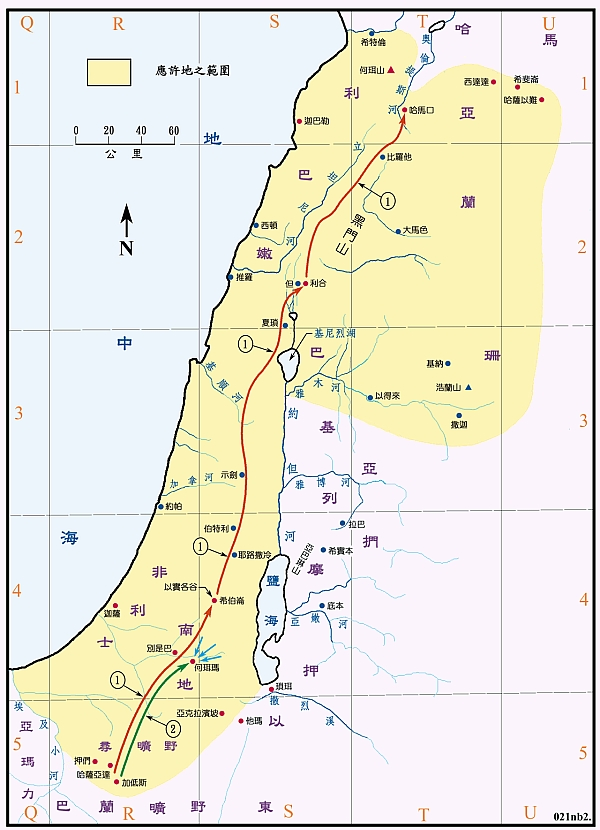
\includegraphics[width=3.8in]{AMoXiFigs/minshuji/tanzi}
\caption{1,十二探子巡视的路径;\\ 2,擅自攻打迦南人，但被迦南人擊敗}
\label{fig:1} 
\end{center}
\end{wrapfigure}
他們上去窺探那地，從尋的曠野到利合，直到哈馬口。他們從南地上去，到了希伯崙，在那裡有亞衲族人亞希幔、示篩、撻買。（原來希伯崙城被建造比埃及的鎖安城早七年。）他們到了以實各谷，從那裡砍了葡萄樹的一枝，上頭有一掛葡萄，兩個人用槓抬著，又帶了些石榴和無花果來。因為以色列人從那裡砍來的那掛葡萄，所以那地方叫做以實各谷。

\subsubsection{探子回來汇报 13:25-29}
過了四十天，他們窺探那地才回來。到了巴蘭曠野的加低斯，見摩西、亞倫並以色列的全會眾，回報摩西、亞倫並全會眾，又把那地的果子給他們看。又告訴摩西說：「我們到了你所打發我們去的那地，果然是流奶與蜜之地。這就是那地的果子。然而住那地的民強壯，城邑也堅固寬大，並且我們在那裡看見了亞衲族的人。亞瑪力人住在南地，赫人、耶布斯人、亞摩利人住在山地，迦南人住在海邊並約旦河旁。」

\subsubsection{迦勒安撫百姓 13:30-31}
迦勒在摩西面前安撫百姓，說：「我們立刻上去得那地吧，我們足能得勝！」但那些和他同去的人說：「我們不能上去攻擊那民，因為他們比我們強壯。」

\subsubsection{探子中有人報惡信 13:32-33}
探子中有人論到所窺探之地，向以色列人報惡信，說：「我們所窺探經過之地是吞吃居民之地，我們在那裡所看見的人民都身量高大。我們在那裡看見亞衲族人，就是偉人，他們是偉人的後裔。據我們看，自己就如蚱蜢一樣；據他們看，我們也是如此。」

\subsubsection{會眾大聲喧嚷百姓都哭號 14:1-4}
當下全會眾大聲喧嚷，那夜百姓都哭號。以色列眾人向摩西、亞倫發怨言，全會眾對他們說：「\textcolor{blue}{巴不得我們早死在埃及地，或是死在這曠野！耶和華為什麼把我們領到那地，使我們倒在刀下呢？我們的妻子和孩子必被擄掠。我們回埃及去豈不好嗎}？」眾人彼此說：「\textcolor{blue}{我們不如立一個首領回埃及去吧}！」

\subsubsection{約書亞和迦勒的信心 14:5-9}
\textcolor{blue}{摩西、亞倫}就俯伏在以色列全會眾面前。窺探地的人中，\textcolor{blue}{嫩的兒子約書亞}和\textcolor{blue}{耶孚尼的兒子迦勒}撕裂衣服，對以色列全會眾說：「我們所窺探經過之地是極美之地。耶和華若喜悅我們，就必將我們領進那地，把地賜給我們，那地原是流奶與蜜之地。但你們不可背叛耶和華，也不要怕那地的居民，因為他們是我們的食物，並且蔭庇他們的已經離開他們。有耶和華與我們同在，不要怕他們。」

\subsubsection{耶和華怒民違逆欲殲滅之 14:10-12}
但\textcolor{blue}{全會眾}說拿石頭打死他們二人。忽然，\textcolor{blue}{耶和華的榮光}在會幕中向以色列眾人顯現。\textcolor{blue}{耶和華對摩西說}：「這百姓藐視我要到幾時呢？我在他們中間行了這一切神蹟，他們還不信我要到幾時呢？我要用瘟疫擊殺他們，使他們不得承受那地，叫你的後裔成為大國，比他們強盛。」

\subsubsection{摩西為民求赦 14:13-19}
摩西對耶和華說：「\textcolor{blue}{埃及人必聽見}這事，因為你曾施展大能，將這百姓從他們中間領上來。埃及人要將這事傳給迦南地的居民。\textcolor{blue}{那民已經聽見}你耶和華是在這百姓中間，因為你面對面被人看見，有你的雲彩停在他們以上，你日間在雲柱中，夜間在火柱中，在他們前面行。如今你若把這百姓殺了，如殺一人，那些聽見你名聲的列邦必議論說：『耶和華因為不能把這百姓領進他向他們起誓應許之地，所以在曠野把他們殺了。』現在\textcolor{red}{求主}大顯能力，照你所說過的話說： 『耶和華不輕易發怒，並有豐盛的慈愛，赦免罪孽和過犯，萬不以有罪的為無罪，必追討他的罪，自父及子，直到三四代。』\textcolor{red}{求你}照你的大慈愛赦免這百姓的罪孽，好像你從埃及到如今常赦免他們一樣。」

\subsubsection{耶和華赦免百姓應許迦勒必得地為業 14:20-25}
耶和華說：「我照著你的話\textcolor{blue}{赦免了他們}。 然我指著我的永生起誓：遍地要被我的榮耀充滿！ 這些人雖看見我的榮耀和我在埃及與曠野所行的神蹟，仍然試探我這十次，不聽從我的話，\textcolor{blue}{他們斷不得看見}我向他們的祖宗所起誓應許之地。凡藐視我的，一個也不得看見。\\
\textcolor{red}{唯獨我的僕人迦勒}，因他另有一個心志，專一跟從我，我就把他領進他所去過的那地。\textcolor{red}{他的後裔}也必得那地為業。亞瑪力人和迦南人住在谷中，明天你們要轉回，從紅海的路往曠野去。」

\subsubsection{以色列眾發怨言者必死於野 14:26-35}
耶和華對摩西、亞倫說：「這惡會眾向我發怨言，我忍耐他們要到幾時呢？以色列人向我所發的怨言，我都聽見了。你們告訴他們：『耶和華說：我指著我的永生起誓：我必要照你們達到我耳中的話待你們。你們的屍首必倒在這曠野，並且你們中間凡被數點，從二十歲以外，向我發怨言的，必不得進我起誓應許叫你們住的那地。唯有耶孚尼的兒子迦勒和嫩的兒子約書亞才能進去。但你們的婦人孩子，就是你們所說要被擄掠的，我必把他們領進去，他們就得知你們所厭棄的那地。至於你們，你們的屍首必倒在這曠野。你們的兒女必在曠野漂流四十年，擔當你們淫行的罪，直到你們的屍首在曠野消滅。 按你們窺探那地的四十日，一年頂一日，你們要擔當罪孽四十年，就知道我與你們疏遠了。』我耶和華說過，我總要這樣待這一切聚集敵我的惡會眾。他們必在這曠野消滅，在這裡死亡。」

\subsubsection{十个報惡信探子遭瘟疫而死 14:36-38}
摩西所打發窺探那地的人回來，報那地的惡信，叫全會眾向摩西發怨言，這些報惡信的人都遭瘟疫，死在耶和華面前。其中唯有嫩的兒子約書亞和耶孚尼的兒子迦勒仍然存活。

\subsubsection{逆命的百姓欲上應許之地被殺退 14:39-45}
摩西將這些話告訴以色列眾人，他們就甚悲哀。清早起來，上山頂去，說：「我們在這裡，我們有罪了。情願上上耶和華所應許的地方去！」摩西說：「你們為何違背耶和華的命令呢？這事不能順利了！不要上去，因為耶和華不在你們中間，恐怕你們被仇敵殺敗了。亞瑪力人和迦南人都在你們面前，你們必倒在刀下。因你們退回不跟從耶和華，所以他必不與你們同在。」他們卻擅敢上山頂去，然而耶和華的約櫃和摩西沒有出營。於是亞瑪力人和住在那山上的迦南人都下來擊打他們，把他們殺退了，直到何珥瑪。

%\section{頒布律法 15 }
\subsection{頒布有關獻祭的條例 15}
\subsubsection{曉諭以色列人獻燔祭,平安祭 15:1-3}
耶和華對摩西說：「你曉諭以色列人說：你們到了我所賜給你們居住的地，若願意從牛群羊群中取牛羊做火祭獻給耶和華，無論是燔祭是平安祭，為要還特許的願，或是做甘心祭，或是逢你們節期獻的，都要奉給耶和華為馨香之祭。

\subsubsection{馨香火祭的條例 15:4-12}
\begin{wraptable}{r}{7cm}
\vspace*{-3mm}
\centering
\begin{tabular}{|c|c|c|c|}
\hline
\hline
\multirow{2}{3em}{祭物} &\multicolumn{2}{c|}{所配的素祭}&\multirow{2}{3em}{奠祭的酒(欣)} \\\cline{2-3}
  & 細麵(伊法)        &油(欣)              &\\ \hline
綿羊羔   &$\sfrac{1}{10}$ &$1\sfrac{1}{4}$&$1\sfrac{1}{4}$\\\hline
公綿羊   &$\sfrac{2}{10}$  &$1\sfrac{1}{3}$ &$1\sfrac{1}{3}$\\\hline
公牛      &$\sfrac{3}{10}$ &$\sfrac{1}{2}$    &$\sfrac{1}{2}$\\\hline
\end{tabular}
\caption{燔祭,平安祭,還特許的願\\所配的素祭和奠祭的酒}
\end{wraptable}
那獻供物的就要將細麵伊法十分之一，並油一欣四分之一，調和做素祭，獻給耶和華。無論是燔祭是平安祭，你要為每隻綿羊羔一同預備奠祭的酒一欣四分之一；為公綿羊預備細麵伊法十分之二，並油一欣三分之一，調和做素祭，又用酒一欣三分之一做奠祭，獻給耶和華為馨香之祭。你預備公牛做燔祭或是做平安祭，為要還特許的願，或是做平安祭，獻給耶和華，就要把細麵伊法十分之三，並油半欣，調和做素祭，和公牛一同獻上，又用酒半欣做奠祭，獻給耶和華為馨香的火祭。獻公牛、公綿羊、綿羊羔、山羊羔，每隻都要這樣辦理。照你們所預備的數目，按著隻數都要這樣辦理。

\subsubsection{同居的外人都歸一例 15:13-16}
凡本地人將馨香的火祭獻給耶和華，都要這樣辦理。若有外人和你們同居，或有人世世代代住在你們中間，願意將馨香的火祭獻給耶和華，你們怎樣辦理，他也要照樣辦理。至於會眾，你們和同居的外人都歸一例，作為你們世世代代永遠的定例。在耶和華面前，你們怎樣，寄居的也要怎樣。你們並與你們同居的外人當有一樣的條例，一樣的典章。

\subsubsection{舉祭的條例 15:17-21}
耶和華對摩西說：你曉諭以色列人說：你們到了我所領你們進去的那地，吃那地的糧食，就要把舉祭獻給耶和華。你們要用初熟的麥子磨麵，做餅當舉祭奉獻，你們舉上，好像舉禾場的舉祭一樣。你們世世代代要用初熟的麥子磨麵，當舉祭獻給耶和華。

\subsubsection{以色列全會眾誤犯罪獻祭的條例 15:22-26}
你們有錯誤的時候，不守耶和華所曉諭摩西的這一切命令，就是耶和華藉摩西一切所吩咐你們的，自那日以至你們的世世代代，若有誤行，是會眾所不知道的，後來全會眾就要
\vspace*{-2mm}
\begin{itemize} 
\itemsep-.35em
\item 將一隻公牛犢做燔祭，並照典章把素祭和奠祭一同獻給耶和華為馨香之祭，
\item 又獻一隻公山羊做贖罪祭。祭司要為以色列全會眾贖罪，
\end{itemize}
\vspace*{-2mm}
他們就必蒙赦免，因為這是錯誤。他們又因自己的錯誤，把供物，就是向耶和華獻的火祭和贖罪祭，一併奉到耶和華面前。以色列全會眾和寄居在他們中間的外人就必蒙赦免，因為這罪是百姓誤犯的。

\subsubsection{一個人誤犯罪獻祭的條例 15:27-29}
若有一個人誤犯了罪，他就要獻一歲的母山羊做贖罪祭。那誤行的人犯罪的時候，祭司要在耶和華面前為他贖罪，他就必蒙赦免。以色列中的本地人和寄居在他們中間的外人，若誤行了什麼事，必歸一樣的條例。

%\subsection{獻祭也不得赦免的罪 15:30-31 }
\subsubsection{違背耶和華的命令的總要剪除 15:30-31}
但那擅敢行事的，無論是本地人是寄居的，他褻瀆了耶和華，必從民中剪除。因他藐視耶和華的言語，違背耶和華的命令，那人總要剪除。他的罪孽要歸到他身上。

\subsubsection{違反安息日的條例 15:32-36 }
以色列人在曠野的時候，遇見一個人在安息日撿柴。遇見他撿柴的人，就把他帶到摩西、亞倫並全會眾那裡，將他收在監內，因為當怎樣辦他，還沒有指明。耶和華吩咐摩西說：「總要把那人治死，全會眾要在營外用石頭把他打死。」於是全會眾將他帶到營外，用石頭打死他，是照耶和華所吩咐摩西的。

\subsubsection{衣服繸子的條例 15:37-41 }
耶和華曉諭摩西說：「你吩咐以色列人，叫他們世世代代在衣服邊上做穗子，又在底邊的穗子上釘一根藍細帶子。你們佩戴這穗子，好叫你們看見就記念遵行耶和華一切的命令，不隨從自己的心意眼目行邪淫，像你們素常一樣，使你們記念遵行我一切的命令，成為聖潔，歸於你們的神。我是耶和華你們的神，曾把你們從埃及地領出來，要做你們的神。我是耶和華你們的神。」

%\section{安營時發生的事 16-17 }
\subsection{可拉黨叛亂 16-17}
\subsubsection{可拉並以色列會中250首領叛逆 16:1-3}
\begin{wraptable}{r}{9cm}
\vspace*{-20mm}
\centering
\begin{tabular}{|c|c|c|c|}
\hline
\hline
支派 & 父親名字&背叛人的名字&  結局 \\ \hline\hline
利未 &哥轄的兒子以斯哈 & 可拉 &被地開口吞沒\\ \hline
流便 & 以利押    &大坍&被地開口吞沒\\\hline
流便 & 以利押    &亞比蘭&被地開口吞沒\\\hline
流便 & 比勒    &安&被地開口吞沒\\\hline
以色列& -& 250個眾首領 &被火燒滅\\\hline
以色列& -& 14700百姓 &被瘟疫所殺\\\hline\hline
\end{tabular}
\caption{背叛的人}
\end{wraptable}
利未的曾孫、哥轄的孫子、以斯哈的兒子可拉，和魯本子孫中以利押的兒子大坍、亞比蘭，與比勒的兒子安，並以色列會中的二百五十個首領，就是有名望選入會中的人，在摩西面前一同起來，聚集攻擊摩西、亞倫，說：「你們擅自專權。全會眾個個既是聖潔，耶和華也在他們中間，你們為什麼自高，超過耶和華的會眾呢？」

\subsubsection{摩西两次劝慰可拉和他一黨的人 16:4-11}
摩西聽見這話就俯伏在地，對可拉和他一黨的人說：「到了早晨，耶和華必指示誰是屬他的，誰是聖潔的，就叫誰親近他。他所揀選的是誰，必叫誰親近他。可拉啊，你們要這樣行：你和你的一黨要拿香爐來，明日在耶和華面前，把火盛在爐中，把香放在其上。耶和華揀選誰，誰就為聖潔。你們這利未的子孫擅自專權了！」 
摩西又對可拉說：「利未的子孫哪，你們聽我說。以色列的神從以色列會中將你們分別出來，使你們親近他，辦耶和華帳幕的事，並站在會眾面前替他們當差。耶和華又使你，和你一切弟兄利未的子孫，一同親近他，這豈為小事，你們還要求祭司的職任嗎？你和你一黨的人聚集是要攻擊耶和華，亞倫算什麼，你們竟向他發怨言呢？」

\subsubsection{流便首領大坍、亞比蘭抗摩西命 16:12-14}
摩西打發人去召以利押的兒子大坍、亞比蘭。他們說：「我們不上去。你將我們從流奶與蜜之地領上來，要在曠野殺我們，這豈為小事，你還要自立為王轄管我們嗎？並且你沒有將我們領到流奶與蜜之地，也沒有把田地和葡萄園給我們為業。難道你要剜這些人的眼睛嗎？我們不上去。」

\subsubsection{亞倫和可拉黨250人各拿香爐全會眾在會幕門前 16:15-19}
摩西就甚發怒，對耶和華說：「求你不要享受他們的供物。我並沒有奪過他們一匹驢，也沒有害過他們一個人。」摩西對可拉說：「明天你和你一黨的人，並亞倫，都要站在耶和華面前。各人要拿一個香爐，共二百五十個，把香放在上面，到耶和華面前。你和亞倫也各拿自己的香爐。」於是他們各人拿一個香爐，盛上火，加上香，同摩西、亞倫站在會幕門前。可拉招聚全會眾到會幕門前，要攻擊摩西、亞倫。

\subsubsection{摩西、亞倫为全會眾代求 16:20-22}
耶和華的榮光就向全會眾顯現。耶和華曉諭摩西、亞倫說：「你們離開這會眾，我好在轉眼之間把他們滅絕。」摩西、亞倫就俯伏在地，說：「神，萬人之靈的神啊！一人犯罪，你就要向全會眾發怒嗎？」 

\subsubsection{摩西照神吩咐警戒會眾離開可拉、大坍、亞比蘭帳篷 16:23-27}
耶和華曉諭摩西說：「你吩咐會眾說：你們離開可拉、大坍、亞比蘭帳篷的四圍。」摩西起來，往大坍、亞比蘭那裡去，以色列的長老也隨著他去。他吩咐會眾說：「你們離開這惡人的帳篷吧，他們的物件，什麼都不可摸，恐怕你們陷在他們的罪中，與他們一同消滅。」於是眾人離開可拉、大坍、亞比蘭帳篷的四圍。大坍、亞比蘭帶著妻子、兒女、小孩子，都出來，站在自己的帳篷門口。

\subsubsection{摩西宣布他們活活地墜落陰間 16:28-30}
摩西說：「我行的這一切事本不是憑我自己心意行的，乃是耶和華打發我行的，必有證據使你們知道。這些人死若與世人無異，或是他們所遭的與世人相同，就不是耶和華打發我來的。倘若耶和華創作一件新事，使地開口，把他們和一切屬他們的都吞下去，叫他們活活地墜落陰間，你們就明白這些人是藐視耶和華了。」

\subsubsection{地開口把他們並一切屬可拉的人丁、財物，都吞下去 16:31-34}
摩西剛說完了這一切話，他們腳下的地就開了口，把他們和他們的家眷，並一切屬可拉的人丁、財物，都吞下去。這樣，他們和一切屬他們的都活活地墜落陰間。地口在他們上頭照舊合閉，他們就從會中滅亡。在他們四圍的以色列眾人聽他們呼號，就都逃跑，說：「恐怕地也把我們吞下去！」

\subsubsection{火燒獻香的250人，以利亞撒用香爐的銅包壇 16:35-40}
又有火從耶和華那裡出來，燒滅了那獻香的二百五十個人。耶和華曉諭摩西說：「你吩咐祭司亞倫的兒子以利亞撒從火中撿起那些香爐來，把火撒在別處，因為那些香爐是聖的。把那些犯罪自害己命之人的香爐，叫人錘成片子，用以包壇。那些香爐本是他們在耶和華面前獻過的，所以是聖的，並且可以給以色列人做記號。」於是祭司以利亞撒將被燒之人所獻的銅香爐拿來，人就錘出來，用以包壇，給以色列人做紀念，使亞倫後裔之外的人不得近前來在耶和華面前燒香，免得他遭可拉和他一黨所遭的。這乃是照耶和華藉著摩西所吩咐的。

\subsubsection{以色列全會眾發怨言，摩西、亞倫代求 16:41-45}
第二天，以色列全會眾都向摩西、亞倫發怨言說：「你們殺了耶和華的百姓了！」會眾聚集攻擊摩西、亞倫的時候，向會幕觀看，不料，有雲彩遮蓋了，耶和華的榮光顯現。摩西、亞倫就來到會幕前。耶和華吩咐摩西說：「你們離開這會眾，我好在轉眼之間把他們滅絕。」他們二人就俯伏於地。 

\subsubsection{因發怨言民遭疫癘 16:46-50}
摩西對亞倫說：「拿你的香爐，把壇上的火盛在其中，又加上香，快快帶到會眾那裡，為他們贖罪。因為有憤怒從耶和華那裡出來，瘟疫已經發作了。」亞倫照著摩西所說的拿來，跑到會中，不料，瘟疫在百姓中已經發作了。他就加上香，為百姓贖罪。他站在活人死人中間，瘟疫就止住了。除了因可拉事情死的以外，遭瘟疫死的，共有一萬四千七百人。亞倫回到會幕門口，到摩西那裡，瘟疫已經止住了。

\subsubsection{十二首領按支派各取仗存在法櫃的帳幕內 17:1-7}
耶和華對摩西說：「你曉諭以色列人，從他們手下取杖，每支派一根。從他們所有的首領，按著支派，共取十二根。你要將各人的名字寫在各人的杖上，並要將亞倫的名字寫在利未的杖上，因為各族長必有一根杖。你要把這些杖存在會幕內法櫃前，就是我與你們相會之處。後來我所揀選的那人，他的杖必發芽。這樣，我必使以色列人向你們所發的怨言止息，不再達到我耳中。」於是摩西曉諭以色列人，他們的首領就把杖交給他，按著支派，每首領一根，共有十二根，亞倫的杖也在其中。摩西就把杖存在法櫃的帳幕內，在耶和華面前。

\subsubsection{亞倫之杖發芽開花結熟杏 17:8-11}
第二天，摩西進法櫃的帳幕去。誰知利未族亞倫的杖已經發了芽，生了花苞，開了花，結了熟杏。摩西就把所有的杖從耶和華面前拿出來，給以色列眾人看。他們看見了，各首領就把自己的杖拿去。耶和華吩咐摩西說：「把亞倫的杖還放在法櫃前，給這些背叛之子留做記號。這樣，你就使他們向我發的怨言止息，免得他們死亡。」摩西就這樣行。耶和華怎樣吩咐他，他就怎樣行了。

\subsubsection{以色列說“凡挨近耶和華帳幕的是必死的” 17:12-13}
以色列人對摩西說：「我們死啦！我們滅亡啦！都滅亡啦！凡挨近耶和華帳幕的是必死的。我們都要死亡嗎？」

\subsection{頒布祭司與利未人的律法 18-19 }
\subsubsection{祭司與利未人的職任 18:1-7 }
\noindent
耶和華對亞倫說：「你和你的兒子並你本族的人，要一同擔當干犯聖所的罪孽，你和你的兒子也要一同擔當干犯祭司職任的罪孽。你要帶你弟兄利未人，就是你祖宗支派的人前來，使他們與你聯合，服侍你，只是你和你的兒子，要一同在法櫃的帳幕前供職。他們要守所吩咐你的，並守全帳幕，只是不可挨近聖所的器具和壇，免得他們和你們都死亡。他們要與你聯合，也要看守會幕，辦理帳幕一切的事，只是外人不可挨近你們。你們要看守聖所和壇，免得憤怒再臨到以色列人。我已將你們的弟兄利未人，從以色列人中揀選出來歸耶和華，是給你們為賞賜的，為要辦理會幕的事。你和你的兒子要為一切屬壇和幔子內的事一同守祭司的職任。你們要這樣供職。我將祭司的職任給你們當做賞賜侍奉我。凡挨近的外人必被治死。」

\subsubsection{祭司當得之物  18:8-14 }
耶和華曉諭亞倫說：我已將歸我的舉祭，就是以色列人一切分別為聖的物，交給你經管。因你受過膏，把這些都賜給你和你的子孫，當做永得的份。
\begin{itemize} 
\itemsep-.25em  
\item 以色列人歸給我至聖的供物，就是一切的素祭、贖罪祭、贖愆祭，其中所有存留不經火的，都為至聖之物，要歸給你和你的子孫。你要拿這些當至聖物吃，\textcolor{blue}{凡男丁都可以吃}。你當以此物為聖。
\item 以色列人所獻的舉祭並搖祭都是你的，我已賜給你和你的兒女，當做永得的份。凡在你\textcolor{blue}{家中的潔淨人都可以吃}。凡油中、新酒中、五穀中至好的，就是以色列人所獻給耶和華初熟之物，我都賜給你。凡從他們地上所帶來給耶和華初熟之物，也都要歸於你。你家中的潔淨人都可以吃。以色列中一切永獻的都必歸於你。 
\end{itemize}

\subsubsection{頭生之物 18:15-20}
\begin{itemize} 
\itemsep-.25em  
\item 他們所有奉給耶和華的，連人帶牲畜，凡頭生的，都要歸給你。只是人頭生的，總要贖出來，不潔淨牲畜頭生的也要贖出來。其中在一月之外所當贖的，要照你所估定的價，按聖所的平，用銀子五舍客勒贖出來（一舍客勒是二十季拉）。 
\item 只是頭生的牛，或是頭生的綿羊和山羊，必不可贖，都是聖的，要把牠的血灑在壇上，把牠的脂油焚燒，當做馨香的火祭獻給耶和華。牠的肉必歸你，像被搖的胸、被舉的右腿歸你一樣。凡以色列人所獻給耶和華聖物中的舉祭，我都賜給你和你的兒女，當做永得的份。這是給你和你的後裔，在耶和華面前作為永遠的鹽(不廢壞)約。」
\item 耶和華對亞倫說：你在以色列人的境內不可有產業，在他們中間也不可有份。我就是你的份，是你的產業。
\end{itemize}

\subsubsection{利未人的份 18:21-24}
\begin{itemize} 
\itemsep-.25em  
\item 凡以色列中出產的十分之一，我已賜給利未的子孫為業。因他們所辦的是會幕的事，所以賜給他們為酬他們的勞。
\item 從今以後，以色列人不可挨近會幕，免得他們擔罪而死。唯獨利未人要辦會幕的事，擔當罪孽，這要做你們世世代代永遠的定例。
\item 他們在以色列人中不可有產業。因為以色列人中出產的十分之一，就是獻給耶和華為舉祭的，我已賜給利未人為業，所以我對他們說：在以色列人中不可有產業。」
\end{itemize}

\subsubsection{利未人的奉獻 18:25-32}
耶和華吩咐摩西說：「你曉諭利未人說：你們從以色列人中所取的十分之一，就是我給你們為業的，要再從那十分之一中取十分之一作為舉祭獻給耶和華。這舉祭要算為你們場上的穀，又如滿酒榨的酒。這樣，你們從以色列人中所得的十分之一也要做舉祭獻給耶和華，從這十分之一中，將所獻給耶和華的舉祭歸給祭司亞倫。奉給你們的一切禮物，要從其中將至好的，就是分別為聖的，獻給耶和華為舉祭。所以你要對利未人說：『你們從其中將至好的舉起，這就算為你們場上的糧，又如酒榨的酒。你們和你們家屬隨處可以吃，這原是你們的賞賜，是酬你們在會幕裡辦事的勞。你們從其中將至好的舉起，就不致因這物擔罪。你們不可褻瀆以色列人的聖物，免得死亡。』」

\subsubsection{用紅母牛灰調做除汙穢水 19:1-10}
\noindent
耶和華曉諭摩西、亞倫說： 「耶和華命定律法中的一條律例乃是這樣說：你要吩咐以色列人，把一隻沒有殘疾、未曾負軛、純紅的母牛牽到你這裡來，交給祭司以利亞撒。他必牽到營外，人就把牛宰在他面前。 祭司以利亞撒要用指頭蘸這牛的血，向會幕前面彈七次。人要在他眼前把這母牛焚燒，牛的皮、肉、血、糞都要焚燒。祭司要把香柏木、牛膝草、朱紅色線都丟在燒牛的火中。祭司必不潔淨到晚上，要洗衣服，用水洗身，然後可以進營。 燒牛的人必不潔淨到晚上，也要洗衣服，用水洗身。必有一個潔淨的人收起母牛的灰，存在營外潔淨的地方，為以色列會眾調做除汙穢的水，這本是除罪的。收起母牛灰的人必不潔淨到晚上，要洗衣服。這要給以色列人和寄居在他們中間的外人作為永遠的定例。 

\subsubsection{適用除汙水的人 19:11-16}
\begin{itemize} 
\itemsep-.25em  
\item 摸了人死屍的，就必七天不潔淨。那人到第三天要用這除汙穢的水潔淨自己，第七天就潔淨了。他若在第三天不潔淨自己，第七天就不潔淨了。凡摸了人死屍，不潔淨自己的，就玷汙了耶和華的帳幕，這人必從以色列中剪除。因為那除汙穢的水沒有灑在他身上，他就為不潔淨，汙穢還在他身上。
\item 人死在帳篷裡的條例乃是這樣：凡進那帳篷的和一切在帳篷裡的，都必七天不潔淨。凡敞口的器皿，就是沒有紮上蓋的，也是不潔淨。
\item 無論何人在田野裡摸了被刀殺的，或是屍首，或是人的骨頭，或是墳墓，就要七天不潔淨。
\end{itemize}

\subsubsection{除汙水的使用 19:17-22}
要為這不潔淨的人拿些燒成的除罪灰放在器皿裡倒上活水。必當有一個潔淨的人拿牛膝草蘸在這水中，把水灑在帳篷上和一切器皿並帳篷內的眾人身上，又灑在摸了骨頭，或摸了被殺的，或摸了自死的，或摸了墳墓的那人身上。
\vspace*{-2mm}
\begin{itemize} 
\itemsep-.25em  
\item 第三天和第七天，潔淨的人要灑水在不潔淨的人身上，第七天就使他成為潔淨。那人要洗衣服，用水洗澡，到晚上就潔淨了。
\item 但那汙穢而不潔淨自己的，要將他從會中剪除，因為他玷汙了耶和華的聖所。除汙穢的水沒有灑在他身上，他是不潔淨的。這要給你們作為永遠的定例。
\item 並且那灑除汙穢水的人要洗衣服，凡摸除汙穢水的，必不潔淨到晚上。不潔淨人所摸的一切物就不潔淨，摸了這物的人必不潔淨到晚上。
\end{itemize}

%\section{行程中發生的事 20-27 }
\subsection{旷野漂流中發生的事 20-22}
\subsubsection{正月米利暗死在尋的曠野加低斯 20:1}
\begin{wrapfigure}{r}{0.5\textwidth}
\vspace*{-30mm}
\center 
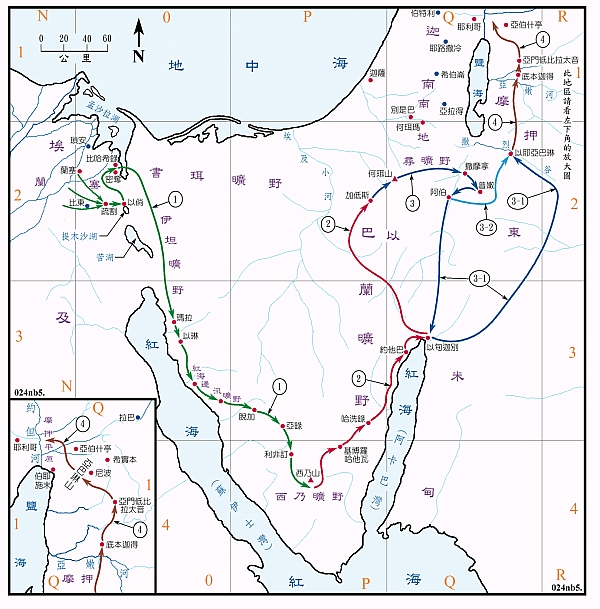
\includegraphics[width=3.5in]{AMoXiFigs/fig4}
\caption{行程中發生的事}
\label{fig:1} 
%\end{center}
\end{wrapfigure}
正月間，以色列全會眾到了尋的曠野，就住在加低斯。米利暗死在那裡，就葬在那裡。


\subsubsection{米利巴摩西因无水受牵累 20:2-13}
\subsubsubsection{米利巴會眾无水攻擊摩西 20:2-5}
會眾沒有水喝，就聚集攻擊摩西、亞倫。百姓向摩西爭鬧說：「我們的弟兄曾死在耶和華面前，我們恨不得與他們同死。你們為何把耶和華的會眾領到這曠野，使我們和牲畜都死在這裡呢？你們為何逼著我們出埃及，領我們到這壞地方呢？這地方不好撒種，也沒有無花果樹、葡萄樹、石榴樹，又沒有水喝。」

\subsubsubsection{曉諭摩西吩咐磐石出水 20:6-9}
摩西、亞倫離開會眾，到會幕門口，俯伏在地。耶和華的榮光向他們顯現。耶和華曉諭摩西說：「你拿著杖去，和你的哥哥亞倫招聚會眾，在他們眼前吩咐磐石發出水來，水就從磐石流出，給會眾和他們的牲畜喝。」

\subsubsubsection{摩西擊打磐石受亏损 20:10-13 }
\begin{table}[H]
%\arrayrulecolor[HTML]{DB5800}
\begin{threeparttable}
\begin{tabular}{@{}p{0.53\textwidth}*{4}{L{\dimexpr0.6\linewidth-10\tabcolsep\relax}}@{}}
\toprule
摩西 &  以東王 \\\hline
於是摩西照耶和華所吩咐的，從耶和華面前取了杖去。摩西、亞倫就招聚會眾到磐石前。摩西說：「你們這些背叛的人聽我說：我為你們使水從這磐石中流出來嗎？」摩西舉手，用杖擊打磐石兩下，就有許多水流出來，會眾和他們的牲畜都喝了。
&耶和華對摩西、亞倫說：「因為你們不信我，不在以色列人眼前尊我為聖，所以你們必不得領這會眾進我所賜給他們的地去。」這水名叫米利巴(爭鬧)水，是因以色列人向耶和華爭鬧，耶和華就在他們面前顯為聖。\tabularnewline
\bottomrule
\end{tabular}
\caption{摩西擊打磐石受亏损}
\end{threeparttable}
\end{table} 

\subsubsection{以東王不允以色列人過其境 20:14-21}
\begin{table}[H]
%\arrayrulecolor[HTML]{DB5800}
\begin{threeparttable}
\begin{tabular}{@{}p{0.53\textwidth}*{4}{L{\dimexpr0.58\linewidth-10\tabcolsep\relax}}@{}}
\toprule
摩西 &  以東王 \\\hline
摩西從加低斯差遣使者去見以東王，說：「你的弟兄以色列人這樣說：我們所遭遇的一切艱難，就是我們的列祖下到埃及，我們在埃及久住，埃及人惡待我們的列祖和我們，我們哀求耶和華的時候，他聽了我們的聲音，差遣使者把我們從埃及領出來，這事你都知道。如今，我們在你邊界上的城加低斯。求你容我們從你的地經過。我們不走田間和葡萄園，也不喝井裡的水，只走大道(王道)，不偏左右，直到過了你的境界。」
&以東王說：「你不可從我的地經過，免得我帶刀出去攻擊你。」\tabularnewline\hline
以色列人說：「我們要走大道上去。我們和牲畜若喝你的水，必給你價值。不求別的，只求你容我們步行過去。」
&以東王說：「你們不可經過。」就率領許多人出來，要用強硬的手攻擊以色列人。這樣，以東王不肯容以色列人從他的境界過去。於是他們轉去，離開他。\tabularnewline
\bottomrule
\end{tabular}
\caption{以東王不允以色列人過其境}
\end{threeparttable}
\end{table} 

\subsubsection{亞倫死在何珥山 20:22-29 }
以色列全會眾從加低斯起行，到了何珥山。耶和華在附近以東邊界的何珥山上曉諭摩西、亞倫說：「亞倫要歸到他列祖(本民)那裡。他必不得入我所賜給以色列人的地，因為在米利巴水，你們違背了我的命。你帶亞倫和他的兒子以利亞撒上何珥山，把亞倫的聖衣脫下來，給他的兒子以利亞撒穿上。亞倫必死在那裡，歸他列祖。」摩西就照耶和華所吩咐的行。三人當著會眾的眼前上了何珥山。摩西把亞倫的聖衣脫下來，給他的兒子以利亞撒穿上，亞倫就死在山頂那裡。於是摩西和以利亞撒下了山。全會眾，就是以色列全家，見亞倫已經死了，便都為亞倫哀哭了三十天。
 
\subsubsection{何珥瑪的迦南人亞拉得王被毀 21:1-3 }
\noindent
南地的迦南人亞拉得王、聽說以色列人從亞他林路來、就和以色列人爭戰、擄了他們幾個人。耶和華應允了以色列人、他們就把迦南人、和迦南人的城邑、盡行毀滅。那地方的名便叫何珥瑪〔毀滅〕。 

\subsubsection{製造銅火蛇  21:5-9 }
他們從何珥山起行，往紅海那條路走，要繞過以東地。百姓因這路難行，心中甚是煩躁，就怨讟神和摩西說：「你們為什麼把我們從埃及領出來，使我們死在曠野呢？這裡沒有糧，沒有水，我們的心厭惡這淡薄的食物！」於是耶和華使火蛇進入百姓中間，蛇就咬他們，以色列人中死了許多。百姓到摩西那裡，說：「我們怨讟耶和華和你，有罪了。求你禱告耶和華，叫這些蛇離開我們。」於是摩西為百姓禱告。耶和華對摩西說：「你製造一條火蛇，掛在杆子上。凡被咬的，一望這蛇，就必得活。」摩西便製造一條銅蛇，掛在杆子上。凡被蛇咬的，一望這銅蛇就活了。

\subsubsection{曠野路線 21:10-20 }
以色列人起行，安營在阿伯。又從阿伯起行，安營在以耶亞巴琳，與摩押相對的曠野，向日出之地。從那裡起行，安營在撒烈谷。從那裡起行，安營在亞嫩河那邊。這亞嫩河是在曠野，從亞摩利的境界流出來的。原來亞嫩河是摩押的邊界，在摩押和亞摩利人搭界的地方。所以《耶和華的戰記》上說：「蘇法的哇哈伯與亞嫩河的谷，並向亞珥城眾谷的下坡，是靠近摩押的境界。」以色列人從那裡起行，到了比珥(井)。從前耶和華吩咐摩西說：「招聚百姓，我好給他們水喝」，說的就是這井。當時，以色列人唱歌說：「井啊，湧上水來！你們要向這井歌唱。這井是首領和民中的尊貴人用圭用杖所挖所掘的。」以色列人從曠野往瑪他拿去，從瑪他拿到拿哈列，從拿哈列到巴末，從巴末到摩押地的谷，又到那下望曠野之毗斯迦的山頂。

\subsubsection{希實本的亞摩利人王西宏 21:21-32}
以色列人差遣使者去見亞摩利人的王西宏，說：「求你容我們從你的地經過。我們不偏入田間和葡萄園，也不喝井裡的水，只走大道 (王道)，直到過了你的境界。」西宏不容以色列人從他的境界經過，就招聚他的眾民出到曠野，要攻擊以色列人，到了雅雜與以色列人爭戰。以色列人用刀殺了他，得了他的地，從亞嫩河到雅博河，直到亞捫人的境界，因為亞捫人的境界多有堅壘。以色列人奪取這一切的城邑，也住亞摩利人的城邑，就是希實本與希實本的一切鄉村。這希實本是亞摩利王西宏的京城，西宏曾與摩押的先王爭戰，從他手中奪取了全地，直到亞嫩河。所以那些作詩歌的說：「你們來到希實本，願西宏的城被修造，被建立！因為有火從希實本發出，有火焰出於西宏的城，燒盡摩押的亞珥和亞嫩河丘壇的祭司(主)。摩押啊，你有禍了！基抹的民哪，你們滅亡了！基抹的男子逃奔，女子被擄，交付亞摩利的王西宏。我們射了他們，希實本直到底本盡皆毀滅。我們使地變成荒場，直到挪法。這挪法直延到米底巴。」這樣，以色列人就住在亞摩利人之地。摩西打發人去窺探雅謝，以色列人就占了雅謝的鎮市，趕出那裡的亞摩利人。

\subsubsection{巴珊王噩 21:33-35}
以色列人轉回，向巴珊去。巴珊王噩和他的眾民都出來，在以得來與他們交戰。耶和華對摩西說：「不要怕他。因我已將他和他的眾民，並他的地，都交在你手中。你要待他像從前待住希實本的亞摩利王西宏一般。」於是他們殺了他和他的眾子，並他的眾民，沒有留下一個，就得了他的地。

\section{摩押平原的事件 22-36}
\subsection{摩押王西撥的兒子召巴勒比珥的兒子巴蘭22-25}

\subsubsection{摩押王西撥的兒子求米甸長老召巴蘭 22:1-6}
以色列人起行，在摩押平原，約旦河東，對著耶利哥安營。以色列人向亞摩利人所行的一切事，西撥的兒子巴勒都看見了。摩押人因以色列民甚多，就大大懼怕，心內憂急，對米甸的長老說：「現在這眾人要把我們四圍所有的一概舔盡，就如牛舔盡田間的草一般。」那時西撥的兒子巴勒做摩押王。他差遣使者往大河邊的毗奪去，到比珥的兒子巴蘭本鄉那裡，召巴蘭來，說：「有一宗民從埃及出來，遮滿地面，與我對居。這民比我強盛，現在求你來為我咒詛他們，或者我能得勝，攻打他們，趕出此地。因為我知道，你為誰祝福，誰就得福；你咒詛誰，誰就受咒詛。」

\subsubsection{一次差摩押米甸長老召巴蘭被拒 22:7-14}
\begin{itemize} 
\itemsep-.35em
\item 摩押的長老和米甸的長老手裡拿著卦金，到了巴蘭那裡，將巴勒的話都告訴了他。巴蘭說：「你們今夜在這裡住宿，我必照耶和華所曉諭我的回報你們。」摩押的使臣就在巴蘭那裡住下了。
\item 神臨到巴蘭那裡，說：「在你這裡的人都是誰？」巴蘭回答說：「是摩押王西撥的兒子巴勒打發人到我這裡來，說： 『從埃及出來的民遮滿地面，你來為我咒詛他們，或者我能與他們爭戰，把他們趕出去。』」神對巴蘭說：「你不可同他們去，也不可咒詛那民，因為那民是蒙福的。」
\item 巴蘭早晨起來，對巴勒的使臣說：「你們回本地去吧，因為耶和華不容我和你們同去。」摩押的使臣就起來，回巴勒那裡去，說：「巴蘭不肯和我們同來。」
\end{itemize}

\subsubsection{二次差更多且尊貴的人召巴蘭 22:15-20}
\begin{itemize} 
\itemsep-.35em
\item 巴勒又差遣使臣，比先前的又多又尊貴。他們到了巴蘭那裡，對他說：「西撥的兒子巴勒這樣說：求你不容什麼事攔阻你不到我這裡來！因為我必使你得極大的尊榮，你向我要什麼，我就給你什麼，只求你來為我咒詛這民。」
\item 巴蘭回答巴勒的臣僕說：「巴勒就是將他滿屋的金銀給我，我行大事小事也不得越過耶和華我神的命。現在我請你們今夜在這裡住宿，等我得知耶和華還要對我說什麼。」
\item 當夜，神臨到巴蘭那裡，說：「這些人若來召你，你就起來同他們去，你只要遵行我對你所說的話。」
\end{itemize}

\subsubsection{天使阻巴蘭 22:21-27}
\begin{table}[H]
\begin{tabular}{@{}p{0.385\textwidth}*{4}{L{\dimexpr0.735\linewidth-10\tabcolsep\relax}}@{}}
\toprule
巴蘭 &驢 \\\hline
巴蘭早晨起來，備上驢，和摩押的使臣一同去了。神因他去就發了怒，耶和華的使者站在路上抵擋他。他騎著驢有兩個僕人跟隨他。&驢看見耶和華的使者站在路上，手裡有拔出來的刀，就從路上跨進田間。\\\hline
巴蘭便打驢，要叫牠回轉上路。&耶和華的使者就站在葡萄園的窄路上，這邊有牆，那邊也有牆。 驢看見耶和華的使者，就貼靠牆，將巴蘭的腳擠傷了。\\\hline
巴蘭又打驢。&耶和華的使者又往前去，站在狹窄之處，左右都沒有轉折的地方。驢看見耶和華的使者，就臥在巴蘭底下，\tabularnewline\hline
巴蘭發怒，用杖打驢。&耶和華叫驢開口對巴蘭說：「我向你行了什麼，你竟打我這三次呢？」\tabularnewline\hline
巴蘭對驢說：「因為你戲弄我。我恨不能手中有刀，把你殺了。」&驢對巴蘭說：「我不是你從小時直到今日所騎的驢嗎？我素常向你這樣行過嗎？」\tabularnewline\hline
巴蘭說：「沒有。」&\tabularnewline\hline
\bottomrule
\end{tabular}
\caption{天使阻巴蘭,驢开口說話}
\end{table} 

\subsubsection{耶和華的使者對巴蘭說話 22:31-35}
\begin{table}[H]
%\begin{threeparttable}
\begin{tabular}{@{}p{0.63\textwidth}*{4}{L{\dimexpr0.48\linewidth-10\tabcolsep\relax}}@{}}
\toprule
耶和華的使者 &  巴蘭 \\\hline
當時，耶和華使巴蘭的眼目明亮，&他就看見耶和華的使者站在路上，手裡有拔出來的刀。巴蘭便低頭俯伏在地。\\\hline
耶和華的使者對他說：「你為何這三次打你的驢呢？我出來抵擋你，因你所行的，在我面前偏僻。驢看見我就三次從我面前偏過去，驢若沒有偏過去，我早把你殺了，留牠存活。」&巴蘭對耶和華的使者說：「我有罪了，我不知道你站在路上阻擋我。你若不喜歡我去，我就轉回。」\\\hline
耶和華的使者對巴蘭說：「你同這些人去吧，你只要說我對你說的話。」&於是巴蘭同著巴勒的使臣去了。\tabularnewline
\bottomrule
\end{tabular}
\caption{耶和華的使者對巴蘭說話}
%\end{threeparttable}
\end{table} 


\subsubsection{巴勒迎巴蘭 22:36-40}
\begin{figure}[H]%{.5\linewidth}
\centering
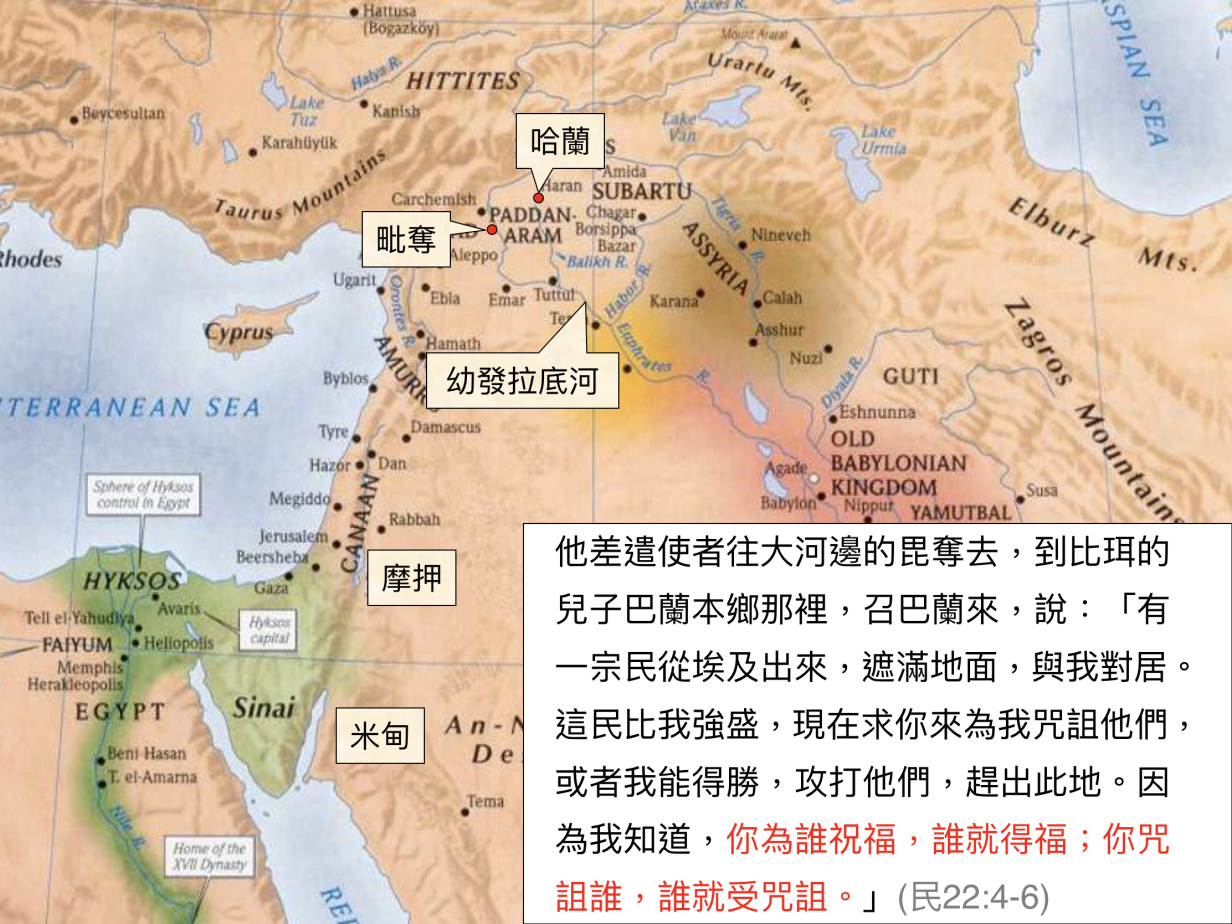
\includegraphics[width=5in]{AMoXiFigs/minshuji/balan}
\caption{以色列在曠野的經歷}
\label{fig:sub1}
\end{figure}
\begin{table}[H]
%\begin{threeparttable}
\begin{tabular}{@{}p{0.5\textwidth}*{4}{L{\dimexpr0.58\linewidth-10\tabcolsep\relax}}@{}}
\toprule
巴勒&巴蘭 \\\hline
巴勒聽見巴蘭來了，就往摩押京城去迎接他。這城是在邊界上，在亞嫩河旁。巴勒對巴蘭說：「我不是急急地打發人到你那裡去召你嗎？你為何不到我這裡來呢？我豈不能使你得尊榮嗎？」&巴蘭說：「我已經到你這裡來了。現在我豈能擅自說什麼呢？神將什麼話傳給我，我就說什麼。」巴蘭和巴勒同行，來到基列胡瑣。巴勒宰（獻）了牛羊，送給巴蘭和陪伴的使臣。\\\hline
\bottomrule
\end{tabular}
\caption{巴勒迎巴蘭}
%\end{threeparttable}
\end{table} 


\subsubsection{巴蘭第一次預言 22:41-23:12}
\begin{table}[H]
\begin{tabular}{@{}p{0.3\textwidth}*{4}{L{\dimexpr0.8\linewidth-10\tabcolsep\relax}}@{}}
\toprule
巴勒&巴蘭 \\\hline
到了早晨，巴勒領巴蘭到巴力的高處，&巴蘭從那裡觀看以色列營的邊界。巴蘭對巴勒說：「你在這裡給我築七座壇，為我預備七隻公牛、七隻公羊。」\\\hline
巴勒照巴蘭的話行了。巴勒和巴蘭在每座壇上獻一隻公牛、一隻公羊。&巴蘭對巴勒說：「你站在你的燔祭旁邊，我且往前去，或者耶和華來迎見我。他指示我什麼，我必告訴你。」於是巴蘭上一淨光的高處。\\\hline
&神迎見巴蘭。巴蘭說：「我預備了七座壇，在每座壇上獻了一隻公牛、一隻公羊。」耶和華將話傳給巴蘭，又說:「你回到巴勒那裡，要如此如此說。」 \\\hline
&他就回到巴勒那裡，見他同摩押的使臣都站在燔祭旁邊。巴蘭便題起詩歌說："巴勒引我出亞蘭，摩押王引我出東山說:『來啊，為我咒詛雅各！來啊，怒罵以色列！』神沒有咒詛的我焉能咒詛？耶和華沒有怒罵的我焉能怒罵？我從高峰看他，從小山望他，這是獨居的民，不列在萬民中。誰能數點雅各的塵土?誰能計算以色列的四分之一?我願如義人之死而死，我願如義人之終而終。"\\\hline
巴勒對巴蘭說：「你向我做的是什麼事呢？我領你來咒詛我的仇敵，不料，你竟為他們祝福！」&他回答說：「耶和華傳給我的話，我能不謹慎傳說嗎？」\\\hline
\bottomrule
\end{tabular}
\caption{巴蘭第一次預言}
\end{table} 



\subsubsection{巴蘭第二次預言 23:13-26}
\begin{table}[H]
%\begin{threeparttable}
\begin{tabular}{@{}p{0.5\textwidth}*{4}{L{\dimexpr0.63\linewidth-10\tabcolsep\relax}}@{}}
\toprule
巴勒&巴蘭 \\\hline
巴勒說：「求你同我往別處去，在那裡可以看見他們。你不能全看見，只能看見他們邊界上的人。在那裡要為我咒詛他們。」於是領巴蘭到了瑣腓田，上了毗斯迦山頂，築了七座壇，每座壇上獻一隻公牛、一隻公羊。&巴蘭對巴勒說：「你站在這燔祭旁邊，等我往那邊去迎見耶和華。」耶和華臨到巴蘭那裡，將話傳給他，又說：「你回到巴勒那裡，要如此如此說。」他就回到巴勒那裡，見他站在燔祭旁邊，摩押的使臣也和他在一處。\\\hline
巴勒問他說：「耶和華說了什麼話呢？」&巴蘭就題詩歌說：「巴勒，你起來聽；西撥的兒子，你聽我言。神非人，必不至說謊；也非人子，必不至後悔。他說話豈不照著行呢？他發言豈不要成就呢？我奉命祝福，神也曾賜福，此事我不能翻轉。他未見雅各中有罪孽，也未見以色列中有奸惡。耶和華他的神和他同在，有歡呼王的聲音在他們中間。神領他們出埃及，他們似乎有野牛之力。斷沒有法術可以害雅各，也沒有占卜可以害以色列。現在必有人論及雅各，就是論及以色列說：『神為他行了何等的大事！』這民起來彷彿母獅，挺身好像公獅，未曾吃野食，未曾喝被傷者之血，決不躺臥。」\\\hline
巴勒對巴蘭說：「你一點不要咒詛他們，也不要為他們祝福。」&巴蘭回答巴勒說：「我豈不是告訴你說，凡耶和華所說的，我必須遵行嗎？」\\\hline
\bottomrule
\end{tabular}
\caption{巴蘭第二次預言}
%\end{threeparttable}
\end{table} 


\subsubsection{巴蘭第三次預言 23:27-24:13}
\begin{table}[H]
%\begin{threeparttable}
\begin{tabular}{@{}p{0.5\textwidth}*{4}{L{\dimexpr0.63\linewidth-10\tabcolsep\relax}}@{}}
\toprule
巴勒&巴蘭 \\\hline
巴勒對巴蘭說：「來吧，我領你往別處去，或者神喜歡你在那裡為我咒詛他們。」巴勒就領巴蘭到那下望曠野的毗珥山頂上。&巴蘭對巴勒說：「你在這裡為我築七座壇，又在這裡為我預備七隻公牛、七隻公羊。」\\\hline
巴勒就照巴蘭的話行，在每座壇上獻一隻公牛、一隻公羊。&巴蘭見耶和華喜歡賜福於以色列，就不像前兩次去求法術，卻面向曠野。巴蘭舉目，看見以色列人照著支派居住，神的靈就臨到他身上，他便題起詩歌說：「比珥的兒子巴蘭說，眼目閉住（（睜開））的人說，得聽神的言語、得見全能者的異象、眼目睜開而仆倒的人說：雅各啊，你的帳篷何等華美！以色列啊，你的帳幕何其華麗！如接連的山谷，如河旁的園子，如耶和華所栽的沉香樹，如水邊的香柏木。水要從他的桶裡流出，種子要撒在多水之處。他的王必超過亞甲，他的國必要振興。神領他出埃及，他似乎有野牛之力。他要吞吃敵國，折斷他們的骨頭，用箭射透他們。他蹲如公獅，臥如母獅，誰敢惹他？凡給你祝福的，願他蒙福；凡咒詛你的，願他受咒詛。」\\\hline
巴勒向巴蘭生氣，就拍起手來，對巴蘭說：「我召你來為我咒詛仇敵，不料，你這三次竟為他們祝福。如今你快回本地去吧！我想使你得大尊榮，耶和華卻阻止你不得尊榮。」&巴蘭對巴勒說：「我豈不是對你所差遣到我那裡的使者說，巴勒就是將他滿屋的金銀給我，我也不得越過耶和華的命，憑自己的心意行好行歹？耶和華說什麼，我就要說什麼。\\\hline
\bottomrule
\end{tabular}
\caption{巴蘭第三次預言}
%\end{threeparttable}
\end{table} 

\subsubsection{巴蘭第四次預言 24:14-25}
\begin{itemize} 
\itemsep-.35em
\item 現在我要回本族去。你來，我告訴你這民日後要怎樣待你的民。」他就題起詩歌說：「比珥的兒子巴蘭說，眼目閉住（睜開）的人說，得聽神的言語、明白至高者的意旨、看見全能者的異象、眼目睜開而仆倒的人說：我看他卻不在現時，我望他卻不在近日。有星要出於雅各，有杖要興於以色列，必打破摩押的四角，毀壞擾亂之子。他必得以東為基業，又得仇敵之地西珥為產業，以色列必行事勇敢。有一位出於雅各的，必掌大權，他要除滅城中的餘民。」
\item 巴蘭觀看亞瑪力，就題起詩歌說：「亞瑪力原為諸國之首，但他終必沉淪。」
\item 巴蘭觀看基尼人，就題起詩歌說：「你的住處本是堅固，你的窩巢做在巖穴中。然而基尼必至衰微，直到亞述把你擄去。」
\item 巴蘭又題起詩歌說：「哀哉！神行這事，誰能得活？必有人乘船從基提界而來，苦害亞述，苦害希伯，他也必至沉淪。」於是巴蘭起來，回他本地去。巴勒也回去了。
\end{itemize} 

%\subsection{百姓在什亭行淫亂 25 }
\subsubsection{百姓與摩押女子在什亭行淫亂 25:1-5}
以色列人住在什亭，百姓與摩押女子行起淫亂。因為這女子叫百姓來，一同給她們的神獻祭，百姓就吃她們的祭物，跪拜她們的神。以色列人與巴力毗珥聯合，耶和華的怒氣就向以色列人發作。耶和華吩咐摩西說：「將百姓中所有的族長在我面前對著日頭懸掛，使我向以色列人所發的怒氣可以消了。」於是摩西吩咐以色列的審判官說：「凡屬你們的人，有與巴力毗珥聯合的，你們各人要把他們殺了。」




\subsubsection{非尼哈刺透行淫亂的二人止息瘟疫 25:6-9}
摩西和以色列全會眾正在會幕門前哭泣的時候，誰知，有以色列中的一個人，當他們眼前，帶著一個米甸女人到他弟兄那裡去。祭司亞倫的孫子、以利亞撒的兒子非尼哈看見了，就從會中起來，手裡拿著槍，跟隨那以色列人進亭子裡去，便將以色列人和那女人由腹中刺透。這樣，在以色列人中瘟疫就止息了。那時遭瘟疫死的有二萬四千人。

\subsubsection{神賜非尼哈後裔永遠當祭司的職任 25:10-13}
耶和華曉諭摩西說：「祭司亞倫的孫子、以利亞撒的兒子非尼哈，使我向以色列人所發的怒消了，因他在他們中間，以我的忌邪為心，使我不在忌邪中把他們除滅。因此，你要說：我將我平安的約賜給他，這約要給他和他的後裔，作為永遠當祭司職任的約，因他為神，有忌邪的心，為以色列人贖罪。」

\subsubsection{行淫亂的以色列人和米甸女人 25:14-15}
那與米甸女人一同被殺的以色列人，名叫心利，是撒路的兒子，是西緬一個宗族的首領。那被殺的米甸女人，名叫哥斯比，是蘇珥的女兒。這蘇珥是米甸一個宗族的首領。

\newpage
\subsubsection{耶和華曉諭摩西擊殺米甸 25:16-18}
\begin{wraptable}{r}{9cm}
\vspace*{-15mm}
\centering
\begin{tabular}{|c|c|c|c|c|}\hline\hline
位置 & 支派 & 第一次人數&第二次人數&  增減 \\ \hline\hline
\multirow{3}{*}{南營} & 流便 & 46500 & 43730  &-2270\\ \cline{2-5}
\multicolumn{1}{|c|}{}  &西緬 & 59300 & 22200 &-37100 \\\cline{2-5}
\multicolumn{1}{|c|}{}  &迦得&45650&40500&-5600\\\cline{2-5}
\hline
\multirow{3}{*}{東營} &猶大 & 57400    &76500& +19100\\\cline{2-5}
\multicolumn{1}{|c|}{} & 以薩迦& 54400&64300&+9900\\\cline{2-5}
\multicolumn{1}{|c|}{} & 西布倫&57400&60500&+3100\\\cline{2-5}
\hline
\multirow{3}{*}{西營} &瑪拿西&32200&52700&+20500\\\cline{2-5}
\multicolumn{1}{|c|}{} & 以法蓮&40500&32500&-8000\\\cline{2-5}
\multicolumn{1}{|c|}{} & 便雅憫&35400&45600&+10200 \\\cline{2-5}
\hline
\multirow{3}{*}{北營} &但&62700&64400&+2700\\\cline{2-5}
\multicolumn{1}{|c|}{} & 亞設&41500&53400&+11900\\\cline{2-5}
\multicolumn{1}{|c|}{} & 拿弗他利&53400&45400&-8000\\\cline{2-5}
\hline
\textbf{總數} & \textbf{以色列} & \textbf{603550}  & \textbf{601730} &
 \textbf{\textcolor{red}{-1820}}\\\hline
 & 利未& 22000 & 23000 & +1000\\\hline
\end{tabular}
\caption{第二次人數 26:1-26 }
\end{wraptable}
耶和華曉諭摩西說：「你要擾害米甸人，擊殺他們。因為他們用詭計擾害你們，在毗珥的事上和他們的姐妹米甸首領的女兒哥斯比的事上，用這詭計誘惑了你們。」這哥斯比，當瘟疫流行的日子，因毗珥的事被殺了。


\subsection{第二次數點以色列人 26:1-65}
\subsubsection{耶和華曉諭摩西以利亞撒二次點人 26:1-4}
瘟疫之後，耶和華曉諭摩西和祭司亞倫的兒子以利亞撒說： 「你們要將以色列全會眾，按他們的宗族，凡以色列中從二十歲以外，能出去打仗的，計算總數。」 摩西和祭司以利亞撒在摩押平原與耶利哥相對的約旦河邊向以色列人說： 「將你們中間從二十歲以外的計算總數，是照耶和華吩咐出埃及地的摩西和以色列人的話。」

\subsubsection{長子流便家族眾子 26:5-11}
\hbox{
\begin{forest}
  for tree={
    child anchor=west,
    parent anchor=east,
    grow=east,
    draw,
    anchor=west,
    edge path={
      \noexpand\path[\forestoption{edge}]
        (.child anchor) -| +(-5pt,0) -- +(-5pt,0) |-
        (!u.parent anchor)\forestoption{edge label};
    },
  }
  [流便
    [哈諾]
    [法路
      [以利押[尼母利][大坍 （可拉一黨的背叛中滅亡）][亞比蘭（可拉一黨的背叛中滅亡）]]
    ]
    [希斯倫] [迦米]
  ]
\end{forest}}
以色列的長子是魯本。魯本的眾子，屬哈諾的，有哈諾族；屬法路的，有法路族； 屬希斯崙的，有希斯崙族；屬迦米的，有迦米族。 這就是魯本的各族。其中被數的，共有四萬三千七百三十名。法路的兒子是以利押。以利押的眾子是尼母利、大坍、亞比蘭。這大坍、亞比蘭，就是從會中選召的，與可拉一黨同向耶和華爭鬧的時候也向摩西、亞倫爭鬧。地便開口吞了他們，和可拉、可拉的黨類一同死亡。那時火燒滅了二百五十個人，他們就做了警戒。然而可拉的眾子沒有死亡。


\subsubsection{西緬家族眾子 26:12-14}
按著家族，西緬的眾子，屬尼母利的，有尼母利族；屬雅憫的，有雅憫族；屬雅斤的，有雅斤族；屬謝拉的，有謝拉族；屬掃羅的，有掃羅族。這就是西緬的各族，共有二萬二千二百名。

\hbox{%\small A small tree (34)
\begin{forest} baseline
 [西緬[尼母利]  [雅憫]  [雅斤]  [謝拉]   [掃羅]]
\end{forest}
\hspace*{10mm}
\normalsize %and
%\large a large tree
\begin{forest} baseline
[迦得 [洗分] [哈基] [書尼] [阿斯尼]  [以利]  [亞律][亞列利]]
\end{forest}
}

\subsubsection{迦得的眾子 26:15-18}
按著家族，迦得的眾子，屬洗分的，有洗分族；屬哈基的，有哈基族；屬書尼的，有書尼族；屬阿斯尼的，有阿斯尼族；屬以利的，有以利族；屬亞律的，有亞律族；屬亞列利的，有亞列利族。這就是迦得子孫的各族，照他們中間被數的，共有四萬零五百名。

\subsubsection{猶大的眾子 26:19-22}
猶大的兒子是珥和俄南。這珥和俄南死在迦南地。 20 按著家族，猶大其餘的眾子，屬示拉的，有示拉族；屬法勒斯的，有法勒斯族；屬謝拉的，有謝拉族。 21 法勒斯的兒子，屬希斯崙的，有希斯崙族；屬哈母勒的，有哈母勒族。 22 這就是猶大的各族，照他們中間被數的，共有七萬六千五百名。


\subsubsection{以薩迦的眾子 26:23-25}
\hbox{
\begin{forest}
  for tree={
    child anchor=west,
    parent anchor=east,
    grow=east,
    draw,
    anchor=west,
    edge path={
      \noexpand\path[\forestoption{edge}]
        (.child anchor) -| +(-5pt,0) -- +(-5pt,0) |-
        (!u.parent anchor)\forestoption{edge label};
    },
  }
  [以薩迦
    [陀拉]  [普瓦]   [雅述]    [伸崙]    ]
\end{forest}
\hspace*{10mm}
\normalsize %and
\begin{forest}
  for tree={
    child anchor=west,
    parent anchor=east,
    grow=east,
    draw,
    anchor=west,
    edge path={
      \noexpand\path[\forestoption{edge}]
        (.child anchor) -| +(-5pt,0) -- +(-5pt,0) |-
        (!u.parent anchor)\forestoption{edge label};
    },
  }
  [猶大
    [珥（死在迦南）]   
    [俄南（死在迦南）]  
    [示拉]  
    [法勒斯 [希斯倫]  [哈母勒	]    ]  
    [謝拉]  
  ]
\end{forest}
\hspace*{10mm}
\begin{forest}
  for tree={
    child anchor=west,
    parent anchor=east,
    grow=east,
    draw,
    anchor=west,
    edge path={
      \noexpand\path[\forestoption{edge}]
        (.child anchor) -| +(-5pt,0) -- +(-5pt,0) |-
        (!u.parent anchor)\forestoption{edge label};
    },
  }
  [西布倫
    [西烈]  [以倫]   [雅利]   ]
\end{forest}
}
按著家族，以薩迦的眾子，屬陀拉的，有陀拉族；屬普瓦的，有普瓦族； 24 屬雅述的，有雅述族；屬伸崙的，有伸崙族。 25 這就是以薩迦的各族，照他們中間被數的，共有六萬四千三百名。

\subsubsection{西布倫的眾子 26:26-27}


按著家族，西布倫的眾子，屬西烈的，有西烈族；屬以倫的，有以倫族；屬雅利的，有雅利族。這就是西布倫的各族，照他們中間被數的，共有六萬零五百名。

\subsubsection{約瑟兒子瑪拿西的眾子 26:28-34}
\begin{forest}
  for tree={
    child anchor=west,
    parent anchor=east,
    grow=east,
    draw,
    anchor=west,
    edge path={
      \noexpand\path[\forestoption{edge}]
        (.child anchor) -| +(-5pt,0) -- +(-5pt,0) |-
        (!u.parent anchor)\forestoption{edge label};
    },
  }
  [瑪拿西
    [瑪吉 
    	[基列 
    	 [伊以謝] [希勒] [亞斯烈] [亞斯烈] [示劍] [示米大] 
    	 [希弗 [西羅非哈 [瑪拉（女兒）] [挪阿（女兒）] [曷拉（女兒）] [密迦（女兒）] [得撒（女兒）]]]    
      ]                                                   
    ]    
  ]
\end{forest}

按著家族，約瑟的兒子有瑪拿西、以法蓮。 瑪拿西的眾子，屬瑪吉的，有瑪吉族。瑪吉生基列，屬基列的，有基列族。基列的眾子，屬伊以謝的，有伊以謝族；屬希勒的，有希勒族；屬亞斯列的，有亞斯列族；屬示劍的，有示劍族；屬示米大的，有示米大族；屬希弗的，有希弗族。希弗的兒子西羅非哈沒兒子，只有女兒，西羅非哈女兒的名字就是瑪拉、挪阿、曷拉、密迦、得撒。這就是瑪拿西的各族，他們中間被數的，共有五萬二千七百名。

\subsubsection{約瑟兒子以法蓮的眾子 26:35-37}
\begin{forest}
  for tree={
    child anchor=west,
    parent anchor=east,
    grow=east,
    draw,
    anchor=west,
    edge path={
      \noexpand\path[\forestoption{edge}]
        (.child anchor) -| +(-5pt,0) -- +(-5pt,0) |-
        (!u.parent anchor)\forestoption{edge label};
    },
  }
  [以法蓮
    [書提拉 [以蘭]] [比結] [他罕]   ]]
\end{forest}

按著家族，以法蓮的眾子，屬書提拉的，有書提拉族；屬比結的，有比結族；屬他罕的，有他罕族；書提拉的眾子，屬以蘭的，有以蘭族。 這就是以法蓮子孫的各族，照他們中間被數的，共有三萬二千五百名。按著家族，這都是約瑟的子孫。

\subsubsection{便雅憫的眾子 26:38-41}
\begin{forest}
  for tree={
    child anchor=west,
    parent anchor=east,
    grow=east,
    draw,
    anchor=west,
    edge path={
      \noexpand\path[\forestoption{edge}]
        (.child anchor) -| +(-5pt,0) -- +(-5pt,0) |-
        (!u.parent anchor)\forestoption{edge label};
    },
  }
  [便雅憫
    [比拉 [亞勒] [乃幔]] 
    [亞實別] [亞希蘭] [書反] [戶反]]
\end{forest}

按著家族，便雅憫的眾子，屬比拉的，有比拉族；屬亞實別的，有亞實別族；屬亞希蘭的，有亞希蘭族；屬書反的，有書反族；屬戶反的，有戶反族。比拉的眾子是亞勒、乃幔；屬亞勒的，有亞勒族；屬乃幔的，有乃幔族。按著家族，這就是便雅憫的子孫，其中被數的，共有四萬五千六百名。

\subsubsection{但的眾子 26:42-43}
\begin{forest}
  for tree={
    child anchor=west,
    parent anchor=east,
    grow=east,
    draw,
    anchor=west,
    edge path={
      \noexpand\path[\forestoption{edge}]
        (.child anchor) -| +(-5pt,0) -- +(-5pt,0) |-
        (!u.parent anchor)\forestoption{edge label};
    },
  }
  [但  [書含]]
\end{forest}

按著家族，但的眾子，屬書含的，有書含族。按著家族，這就是但的各族。照其中被數的，書含所有的各族，共有六萬四千四百名。

\subsubsection{亞設的眾子 26:44-47}
\begin{forest}
  for tree={
    child anchor=west,
    parent anchor=east,
    grow=east,
    draw,
    anchor=west,
    edge path={
      \noexpand\path[\forestoption{edge}]
        (.child anchor) -| +(-5pt,0) -- +(-5pt,0) |-
        (!u.parent anchor)\forestoption{edge label};
    },
  }
  [亞設  [音拿] [亦施韋] [比利亞 [希別] [瑪結]] [西拉（亞設的女兒）]]
\end{forest}

按著家族，亞設的眾子，屬音拿的，有音拿族；屬亦施韋的，有亦施韋族；屬比利亞的，有比利亞族。 比利亞的眾子，屬希別的，有希別族；屬瑪結的，有瑪結族。 亞設的女兒名叫西拉。這就是亞設子孫的各族，照他們中間被數的，共有五萬三千四百名。

\subsubsection{拿弗他利的眾子 26:48-50}
\begin{forest}
  for tree={
    child anchor=west,
    parent anchor=east,
    grow=east,
    draw,
    anchor=west,
    edge path={
      \noexpand\path[\forestoption{edge}]
        (.child anchor) -| +(-5pt,0) -- +(-5pt,0) |-
        (!u.parent anchor)\forestoption{edge label};
    },
  }
  [拿弗他利  [雅薛] [沽尼] [耶色] [示冷]]
\end{forest}

按著家族，拿弗他利的眾子，屬雅薛的，有雅薛族；屬沽尼的，有沽尼族；屬耶色的，有耶色族；屬示冷的，有示冷族。 按著家族，這就是拿弗他利的各族，他們中間被數的，共有四萬五千四百名。

\subsubsection{分地原则-按各支派名字人数多少拈鬮分地 26:51-56}
以色列人中被數的，共有六十萬零一千七百三十名。耶和華曉諭摩西說：「你要按著人名的數目將地分給這些人為業。人多的，你要把產業多分給他們；人少的，你要把產業少分給他們。要照被數的人數，把產業分給各人。雖是這樣，還要拈鬮分地。他們要按著祖宗各支派的名字承受為業。要按著所拈的鬮，看人數多人數少，把產業分給他們。」


\subsubsection{利未的各族被數人 26:57-62}
\begin{forest}
  for tree={
    child anchor=west,
    parent anchor=east,
    grow=east,
    draw,
    anchor=west,
    edge path={
      \noexpand\path[\forestoption{edge}]
        (.child anchor) -| +(-5pt,0) -- +(-5pt,0) |-
        (!u.parent anchor)\forestoption{edge label};
    },
  }
  [利未  
  	[革順 [立尼][\textcolor{red}{示每}]] 
  	[哥轄[暗蘭（妻子-約基別）[亞倫[拿答（獻凡火而死）][亞比戶（獻凡火而死）][以利亞撒][以他瑪]][摩西][米利暗（姐姐）]][希伯倫] [\textcolor{red}{以斯哈}[可拉] ] [\textcolor{red}{烏薛}]  ] 
  	[米拉利 [瑪利][母示]]]
\end{forest}

利未人\footnote{備註：\textcolor{red}{紅色}為第二次數點時消失的支派}，按著他們的各族被數的，屬革順的，有革順族；屬哥轄的，有哥轄族；屬米拉利的，有米拉利族。利未的各族有立尼族、希伯倫族、瑪利族、母示族、可拉族。哥轄生暗蘭。暗蘭的妻名叫約基別，是利未女子，生在埃及。她給暗蘭生了亞倫、摩西，並他們的姐姐米利暗。亞倫生拿答、亞比戶、以利亞撒、以他瑪。拿答、亞比戶在耶和華面前獻凡火的時候就死了。利未人中，凡一個月以外，被數的男丁，共有二萬三千。他們本來沒有數在以色列人中，因為在以色列人中，沒有分給他們產業。

\subsubsection{各族在摩押平原與耶利哥相對的約旦河邊被數點 26:63-65}
這些就是被摩西和祭司以利亞撒所數的。他們在摩押平原與耶利哥相對的約旦河邊數點以色列人。但被數的人中，沒有一個是摩西和祭司亞倫從前在西奈的曠野所數的以色列人。因為耶和華論到他們說，他們必要死在曠野，所以除了耶孚尼的兒子迦勒和嫩的兒子約書亞以外，連一個人也沒有存留。

\subsection{瑪拿西族西羅非哈的女兒們  27:1-11}
\subsubsection{西羅非哈的女兒們求產業  27:1-5}
屬約瑟的兒子瑪拿西的各族，有瑪拿西的玄孫、瑪吉的曾孫、基列的孫子、希弗的兒子西羅非哈的女兒，名叫瑪拉、挪阿、曷拉、密迦、得撒。她們前來，站在會幕門口，在摩西和祭司以利亞撒並眾首領與全會眾面前，說：「我們的父親死在曠野。他不與可拉同黨聚集攻擊耶和華，是在自己罪中死的。他也沒有兒子。為什麼因我們的父親沒有兒子，就把他的名從他族中除掉呢？求你們在我們父親的弟兄中分給我們產業。」 於是摩西將她們的案件呈到耶和華面前。

\subsubsection{耶和華颁布女子得地的律例  27:6-11}
耶和華曉諭摩西說：「西羅非哈的女兒說的有理。你定要在她們父親的弟兄中，把地分給她們為業，要將她們父親的產業歸給她們。你也要曉諭以色列人說：人若死了沒有兒子，就要把他的產業歸給他的女兒；他若沒有女兒，就要把他的產業給他的弟兄；他若沒有弟兄，就要把他的產業給他父親的弟兄；他父親若沒有弟兄，就要把他的產業給他族中最近的親屬，他便要得為業。這要做以色列人的律例、典章，是照耶和華吩咐摩西的。」

\subsection{立嫩的兒子約書亞  27:12-23}
\subsubsection{耶和華曉諭摩西將歸其列祖  27:12-14}
耶和華對摩西說：「你上這亞巴琳山，觀看我所賜給以色列人的地。看了以後，你也必歸到你列祖 （本民）那裡，像你哥哥亞倫一樣。因為你們在尋的曠野，當會眾爭鬧的時候，違背了我的命，沒有在湧水之地會眾眼前尊我為聖。」（這水就是尋的曠野加低斯米利巴水。）

\subsubsection{摩西求耶和華另立一人治理會眾 27:15-17}
摩西對耶和華說：「願耶和華萬人之靈的神，立一個人治理會眾，可以在他們面前出入，也可以引導他們，免得耶和華的會眾如同沒有牧人的羊群一般。」 

\subsubsection{耶和華立嫩的兒子約書亞 27:18-23}
耶和華對摩西說：「嫩的兒子約書亞是心中有聖靈的，你將他領來，按手在他頭上，使他站在祭司以利亞撒和全會眾面前，囑咐他。又將你的尊榮給他幾分，使以色列全會眾都聽從他。他要站在祭司以利亞撒面前，以利亞撒要憑烏陵的判斷，在耶和華面前為他求問。他和以色列全會眾都要遵以利亞撒的命出入。」於是摩西照耶和華所吩咐的將約書亞領來，使他站在祭司以利亞撒和全會眾面前，按手在他頭上，囑咐他，是照耶和華藉摩西所說的話。

%\newpage
\subsection{頒布献祭与许愿律法 28-30 }
\subsubsection{日祭：每日恆獻的燔祭之例 28:1-8}
\begin{wraptable}{r}{10cm}
\centering
\begin{tabular}{|c|c|c|c|}
\hline
\hline
獻祭時間 & 火祭-公羊羔&素祭(細麵+油調和)&  奠祭-酒 \\ \hline\hline
早晨 &沒有殘疾一歲(1) &$\sfrac{1}{10}$伊法+$1\sfrac{1}{4}$欣&$1\sfrac{1}{4}$欣\\ \hline
黃昏 &沒有殘疾一歲(1) &$\sfrac{1}{10}$伊法+$1\sfrac{1}{4}$欣&$1\sfrac{1}{4}$欣\\ \hline
\end{tabular}
\caption{每日獻的燔祭 28:1-8}
\end{wraptable}
耶和華曉諭摩西說：你要吩咐以色列人說：獻給我的供物，就是獻給我做馨香火祭的食物，你們要按日期獻給我。又要對他們說：你們要獻給耶和華的火祭，就是沒有殘疾、一歲的公羊羔，每日兩隻，作為常獻的燔祭。早晨要獻一隻，黃昏的時候要獻一隻。又用細麵伊法十分之一，並搗成的油一欣四分之一，調和作為素祭。這是西奈山所命定為常獻的燔祭，是獻給耶和華為馨香的火祭。為這一隻羊羔，要同獻奠祭的酒一欣四分之一。在聖所中，你要將醇酒奉給耶和華為奠祭。晚上，你要獻那一隻羊羔，必照早晨的素祭和同獻的奠祭獻上，作為馨香的火祭獻給耶和華。

\subsubsection{周祭：安息日獻的燔祭 28:9-10}
\begin{wraptable}{r}{8cm}
\vspace*{-8mm}
\centering
\begin{tabular}{|c|c|c|}
\hline
\hline
 火祭-公羊羔&素祭(細麵+油)&  奠祭 \\ \hline\hline
沒有殘疾一歲的(2) &\sfrac{2}{10}伊法+油調和 &酒\\ \hline
\end{tabular}
\caption{安息日獻的燔祭 28:9-10}
\end{wraptable}
當安息日，要獻兩隻沒有殘疾、一歲的公羊羔，並用調油的細麵伊法十分之二為素祭，又將同獻的奠祭獻上。這是每安息日獻的燔祭，\textcolor{blue}{那常獻的燔祭和同獻的奠祭在外}。

\subsubsection{月朔：燔祭+贖罪祭 28:11-15}
\begin{wraptable}{r}{8.5cm}
\centering
\vspace*{-1mm}
\begin{tabular}{|c|c|c|}
\hline
\hline
 燔祭+贖罪祭牲&素祭-調油細麵&  奠祭-酒 \\ \hline\hline
 公牛犢(2) &\sfrac{3}{10}伊法/隻 &\sfrac{1}{2}欣/隻\\ \hline
 公綿羊(1) &\sfrac{2}{10}伊法/隻 &\sfrac{1}{3}欣/隻\\ \hline
沒有殘疾一歲公羊羔(7) &\sfrac{1}{10}伊法/隻 &\sfrac{1}{4}欣/隻\\ \hline
公山羊(1) &\multicolumn{2}{ c|}{贖罪祭}\\ \hline
\end{tabular}
\caption{月朔獻的燔祭+贖罪祭  28:11-15}
\end{wraptable}
每月朔，你們要將兩隻公牛犢，一隻公綿羊，七隻沒有殘疾、一歲的公羊羔，獻給耶和華為燔祭。每隻公牛要用調油的細麵伊法十分之三作為素祭，那隻公羊也用調油的細麵伊法十分之二作為素祭，每隻羊羔要用調油的細麵伊法十分之一作為素祭和馨香的燔祭，是獻給耶和華的火祭。一隻公牛要奠酒半欣，一隻公羊要奠酒一欣三分之一，一隻羊羔也奠酒一欣四分之一。這是每月的燔祭，一年之中要月月如此。又要將一隻公山羊為贖罪祭，獻給耶和華，要獻在常獻的燔祭和同獻的奠祭以外。


\subsubsection{年祭1-逾越節當獻的祭：燔祭+贖罪祭+每日獻的燔祭 28:16-25}
\begin{wraptable}{r}{9cm}
\centering
\vspace*{-1mm}
\begin{tabular}{|c|c|c|}
\hline
\hline
 日期&燔祭+贖罪祭 & 其他條例\\ \hline\hline
 正月十四日 &表\ref{tab:qiqijie} &有聖會不作工喫無酵餅\\ \hline
 正月十五日 &表\ref{tab:qiqijie} &喫無酵餅\\ \hline
正月十六日  &表\ref{tab:qiqijie}  &喫無酵餅\\ \hline
正月十七日  &表\ref{tab:qiqijie} &喫無酵餅\\ \hline
正月十八日  &表\ref{tab:qiqijie}  &喫無酵餅\\ \hline
正月十九日  &表\ref{tab:qiqijie}  &喫無酵餅\\ \hline
正月二十日  &表\ref{tab:qiqijie} &有聖會不作工喫無酵餅\\ \hline
\end{tabular}
\caption{逾越節獻的祭  28:16-25}
\end{wraptable}
正月十四日是耶和華的逾越節。這月十五日是節期，要吃無酵餅七日。第一日當有聖會，什麼勞碌的工都不可做。當將公牛犢兩隻、公綿羊一隻、一歲的公羊羔七隻，都要沒有殘疾的，用火獻給耶和華為燔祭。同獻的素祭用調油的細麵：為一隻公牛要獻伊法十分之三，為一隻公羊要獻伊法十分之二，為那七隻羊羔每隻要獻伊法十分之一。並獻一隻公山羊做贖罪祭，為你們贖罪。你們獻這些，要在早晨常獻的燔祭以外。一連七日，每日要照這例把馨香火祭的食物獻給耶和華，是在常獻的燔祭和同獻的奠祭以外。第七日當有聖會，什麼勞碌的工都不可做。

\subsubsection{年祭2-七七節獻的祭 28:26-31}
\begin{wraptable}{r}{6.5cm}
\centering
\vspace*{-8mm}
\begin{tabular}{|c|c|}
\hline
\hline
 燔祭&素祭-調油細麵 \\ \hline\hline
 公牛犢(2) &\sfrac{3}{10}伊法/隻 \\ \hline
 公綿羊(1) &\sfrac{2}{10}伊法/隻 \\ \hline 
无殘疾一歲公羊羔(7) &\sfrac{1}{10}伊法/隻 \\ \hline\hline
\multicolumn{2}{ |c|}{公山羊(1) 贖罪祭}\\ \hline
\end{tabular}
\caption{七七節獻的祭}
\label{tab:qiqijie}
\end{wraptable}
七七節莊稼初熟，你們獻新素祭給耶和華的日子，當有聖會，什麼勞碌的工都不可做。只要將公牛犢兩隻、公綿羊一隻、一歲的公羊羔七隻，作為馨香的燔祭獻給耶和華。 同獻的素祭用調油的細麵：為每隻公牛要獻伊法十分之三，為一隻公羊要獻伊法十分之二，為那七隻羊羔每隻要獻伊法十分之一。並獻一隻公山羊為你們贖罪。這些，你們要獻在常獻的燔祭和同獻的素祭並同獻的奠祭以外，都要沒有殘疾的。


\subsubsection{年祭3-新年(吹角日)獻的祭 29:1-6 }
\begin{wraptable}{r}{6.5cm}
\centering
\vspace*{-8mm}
\begin{tabular}{|c|c|}
\hline
\hline
 燔祭&素祭-調油細麵 \\ \hline\hline
 公牛犢(\textcolor{red}{1}) &\sfrac{3}{10}伊法/隻 \\ \hline
 公綿羊(1) &\sfrac{2}{10}伊法/隻 \\ \hline 
无殘疾一歲公羊羔(7) &\sfrac{1}{10}伊法/隻 \\ \hline\hline
\multicolumn{2}{ |c|}{公山羊(1) 贖罪祭}\\ \hline
\end{tabular}
\caption{吹角日獻的祭}
\label{tab:xinnian}
\end{wraptable}
 七月初一日，你們當有聖會，什麼勞碌的工都不可做，是你們當守為吹角的日子。你們要將公牛犢一隻，公綿羊一隻，沒有殘疾、一歲的公羊羔七隻，作為馨香的燔祭獻給耶和華。同獻的素祭用調油的細麵：為一隻公牛要獻伊法十分之三，為一隻公羊要獻伊法十分之二，為那七隻羊羔每隻要獻伊法十分之一。又獻一隻公山羊做贖罪祭，為你們贖罪。這些是在月朔的燔祭和同獻的素祭，並常獻的燔祭與同獻的素祭，以及照例同獻的奠祭以外，都作為馨香的火祭獻給耶和華。

\subsubsection{年祭4-贖罪日獻的祭 29:7-11 }
七月初十日，你們當有聖會，要刻苦己心，什麼工都不可做。 只要將公牛犢一隻、公綿羊一隻、一歲的公羊羔七隻，都要沒有殘疾的，作為馨香的燔祭獻給耶和華。同獻的素祭用調油的細麵：為一隻公牛要獻伊法十分之三，為一隻公羊要獻伊法十分之二，為那七隻羊羔每隻要獻伊法十分之一。又獻一隻公山羊為贖罪祭，這是在贖罪祭和常獻的燔祭，與同獻的素祭並同獻的奠祭以外（獻祭条例同表\ref{tab:xinnian}） 。

\subsubsection{年祭-住棚節獻的祭  29:12-40 }
七月十五日，你們當有聖會，什麼勞碌的工都不可做，要向耶和華守節七日。又要將公牛犢十三隻、公綿羊兩隻、一歲的公羊羔十四隻，都要沒有殘疾的，用火獻給耶和華為馨香的燔祭。 同獻的素祭用調油的細麵：為那十三隻公牛每隻要獻伊法十分之三，為那兩隻公羊每隻要獻伊法十分之二，為那十四隻羊羔每隻要獻伊法十分之一。並獻一隻公山羊為贖罪祭，這是在常獻的燔祭和同獻的素祭並同獻的奠祭以外。

第二日要獻公牛犢十二隻，公綿羊兩隻，沒有殘疾、一歲的公羊羔十四隻。並為公牛、公羊和羊羔，按數照例，獻同獻的素祭和同獻的奠祭。又要獻一隻公山羊為贖罪祭，這是在常獻的燔祭和同獻的素祭並同獻的奠祭以外。

 「第三日要獻公牛十一隻，公羊兩隻，沒有殘疾、一歲的公綿羊羔十四隻。並為公牛、公羊和羊羔，按數照例，獻同獻的素祭和同獻的奠祭。又要獻一隻公山羊為贖罪祭，這是在常獻的燔祭和同獻的素祭並同獻的奠祭以外。

 「第四日要獻公牛十隻，公羊兩隻，沒有殘疾、一歲的公羊羔十四隻。並為公牛、公綿羊和羊羔，按數照例，獻同獻的素祭和同獻的奠祭。又要獻一隻公山羊為贖罪祭，這是在常獻的燔祭和同獻的素祭並同獻的奠祭以外。

「第五日要獻公牛九隻，公羊兩隻，沒有殘疾、一歲的公羊羔十四隻。 27 並為公牛、公羊和羊羔，按數照例，獻同獻的素祭和同獻的奠祭。 28 又要獻一隻公山羊為贖罪祭，這是在常獻的燔祭和同獻的素祭並同獻的奠祭以外。

29 「第六日要獻公牛八隻，公羊兩隻，沒有殘疾、一歲的公羊羔十四隻。 30 並為公牛、公羊和羊羔，按數照例，獻同獻的素祭和同獻的奠祭。 31 又要獻一隻公山羊為贖罪祭，這是在常獻的燔祭和同獻的素祭並同獻的奠祭以外。

32 「第七日要獻公牛七隻，公羊兩隻，沒有殘疾、一歲的公羊羔十四隻。 33 並為公牛、公羊和羊羔，按數照例，獻同獻的素祭和同獻的奠祭。 34 又要獻一隻公山羊為贖罪祭，這是在常獻的燔祭和同獻的素祭並同獻的奠祭以外。

第八日你們當有嚴肅會，什麼勞碌的工都不可做。 36 只要將公牛一隻，公羊一隻，沒有殘疾、一歲的公羊羔七隻做火祭，獻給耶和華為馨香的燔祭。 37 並為公牛、公羊和羊羔，按數照例，獻同獻的素祭和同獻的奠祭。 38 又要獻一隻公山羊為贖罪祭，這是在常獻的燔祭和同獻的素祭並同獻的奠祭以外。

39 「這些祭要在你們的節期獻給耶和華，都在所許的願並甘心所獻的以外，作為你們的燔祭、素祭、奠祭和平安祭。」 40 於是摩西照耶和華所吩咐他的一切話告訴以色列人。

\subsubsection{女子許願的條例 30:1-16 }
\subsubsubsection{女子年幼在父家時候許願的條例 30:1-5}
\begin{wraptable}{r}{6.5cm}
\centering
\vspace*{-8mm}
\begin{tabular}{|c|c|}\hline\hline
 
女子年幼在父家 &父親坚定或废弃誓言 \\ \hline
女子出了嫁       &丈夫坚定或废弃誓言 \\ \hline 
寡婦或离异婦人 &自己坚定或废弃誓言 \\ \hline\hline
\end{tabular}
\caption{女子許願的條例}
\label{tab:xinnian}
\end{wraptable}
摩西曉諭以色列各支派的首領說：耶和華所吩咐的乃是這樣：人若向耶和華許願或起誓，要約束自己，就不可食言，必要按口中所出的一切話行。女子年幼還在父家的時候，若向耶和華許願，要約束自己，她父親也聽見她所許的願並約束自己的話，卻向她默默不言，她所許的願並約束自己的話就都要為定。但她父親聽見的日子若不應承她所許的願和約束自己的話，就都不得為定，耶和華也必赦免她，因為她父親不應承。

\subsubsubsection{女子出了嫁許願的條例 30:6-8}
她若出了嫁，有願在身，或是口中出了約束自己的冒失話，她丈夫聽見的日子，卻向她默默不言，她所許的願並約束自己的話就都要為定。但她丈夫聽見的日子，若不應承，就算廢了她所許的願和她出口約束自己的冒失話，耶和華也必赦免她。

\subsubsubsection{寡婦、或是被休的婦人許願的條例 30:9}
寡婦或是被休的婦人所許的願，就是她約束自己的話，都要為定。 

\subsubsubsection{丈夫可以堅定,廢去妻子許的願 30:10-16}
她若在丈夫家裡許了願或起了誓，約束自己，丈夫聽見，卻向她默默不言，也沒有不應承，她所許的願並約束自己的話就都要為定。丈夫聽見的日子，若把這兩樣全廢了，婦人口中所許的願或是約束自己的話就都不得為定，因她丈夫已經把這兩樣廢了，耶和華也必赦免她。凡她所許的願和刻苦約束自己所起的誓，她丈夫可以堅定，也可以廢去。倘若她丈夫天天向她默默不言，就算是堅定她所許的願和約束自己的話，因丈夫聽見的日子向她默默不言，就使這兩樣堅定。但她丈夫聽見以後，若使這兩樣全廢了，就要擔當婦人的罪孽。這是丈夫待妻子，父親待女兒，女兒年幼還在父家，耶和華所吩咐摩西的律例。



%\section{行程中發生的事  31-34 }
\subsection{與米甸人打仗 31}
\subsubsection{與米甸人打仗 31:1-6}
耶和華吩咐摩西說： 2 「你要在米甸人身上報以色列人的仇，後來要歸到你列祖 a那裡。」 3 摩西吩咐百姓說：「要從你們中間叫人帶兵器出去攻擊米甸，好在米甸人身上為耶和華報仇。 4 從以色列眾支派中，每支派要打發一千人去打仗。」 5 於是從以色列千萬人中，每支派交出一千人，共一萬二千人，帶著兵器預備打仗。 6 摩西就打發每支派的一千人去打仗，並打發祭司以利亞撒的兒子非尼哈同去，非尼哈手裡拿著聖所的器皿和吹大聲的號筒。

\subsubsection{打仗結果 31:7-12}
他們就照耶和華所吩咐摩西的，與米甸人打仗，殺了所有的男丁。 8 在所殺的人中，殺了米甸的五王，就是以未、利金、蘇珥、戶珥、利巴，又用刀殺了比珥的兒子巴蘭。 9 以色列人擄了米甸人的婦女、孩子，並將他們的牲畜、羊群和所有的財物都奪了來，當做擄物。 10 又用火焚燒他們所住的城邑和所有的營寨， 11 把一切所奪的、所擄的，連人帶牲畜都帶了去。 12 將所擄的人，所奪的牲畜、財物，都帶到摩押平原，在約旦河邊與耶利哥相對的營盤，交給摩西和祭司以利亞撒並以色列的會眾。

\subsubsection{处理男孩和女俘虏 31:13-20}
摩西和祭司以利亞撒並會眾一切的首領，都出到營外迎接他們。 14 摩西向打仗回來的軍長，就是千夫長、百夫長發怒， 15 對他們說：「你們要存留這一切婦女的活命嗎？ 16 這些婦女因巴蘭的計謀，叫以色列人在毗珥的事上得罪耶和華，以致耶和華的會眾遭遇瘟疫。 17 所以，你們要把一切的男孩和所有已嫁的女子都殺了。 18 但女孩子中，凡沒有出嫁的，你們都可以存留她的活命。 19 你們要在營外駐紮七日。凡殺了人的，和一切摸了被殺的，並你們所擄來的人口，第三日、第七日，都要潔淨自己， 20 也要因一切的衣服、皮物、山羊毛織的物和各樣的木器，潔淨自己。」

\subsubsection{戰後潔淨條例 31:21-24} 
祭司以利亞撒對打仗回來的兵丁說：「耶和華所吩咐摩西律法中的條例乃是這樣： 22 金、銀、銅、鐵、錫、鉛， 23 凡能見火的，你們要叫它經火就為潔淨，然而還要用除汙穢的水潔淨它。凡不能見火的，你們要叫它過水。 24 第七日，你們要洗衣服，就為潔淨，然後可以進營。」

\subsubsection{耶和華曉諭摩西戰利品的分配原则 31:25-31} 	
耶和華曉諭摩西說： 26 「你和祭司以利亞撒並會眾的各族長，要計算所擄來的人口和牲畜的總數。 27 把所擄來的分做兩半，一半歸於出去打仗的精兵，一半歸於全會眾。 28 又要從出去打仗所得的人口、牛、驢、羊群中，每五百取一，作為貢物奉給耶和華。 29 從他們一半之中，要取出來交給祭司以利亞撒，作為耶和華的舉祭。 30 從以色列人的一半之中，就是從人口、牛、驢、羊群、各樣牲畜中，每五十取一，交給看守耶和華帳幕的利未人。」 31 於是摩西和祭司以利亞撒照耶和華所吩咐摩西的行了。

\subsubsection{统计戰利品，执行耶和華的吩咐 31:32-46}
\begin{wraptable}{r}{11.5cm}
\centering
\begin{tabular}{|c|c|c|c|c|c|}
\hline
\hline
\multicolumn{2}{|c|}{}     &羊    &    牛&  驢   & 女人 \\ \hline\hline 
\multicolumn{2}{|c|}{戰利品總數}           &675000&72000 & 61000 & 32000\\ \cline{2-6}\hline
\multirow{2}{*}{兵丁所得}&1/500歸神& 337500&36000&30500&16000 \\ 
\multicolumn{1}{|c|}{}   &1/2做舉祭歸祭司&675    &72   &61   &32 \\ \cline{2-6}\hline
\multirow{2}{*}{以色列人所得}  && 337500 & 36000 &30500 &  16000 \\ 
\multicolumn{1}{|c|}{}         &1/50歸利未人&6750 & 720 &610 &320 \\ \cline{2-6}\hline
\end{tabular}
\caption{戰利品分配 }
\end{wraptable}
除了兵丁所奪的財物以外，所擄來的：羊六十七萬五千隻，牛七萬二千隻，驢六萬一千匹，女人共三萬二千口，都是沒有出嫁的。\textcolor{blue}{出去打仗之人的份，就是他們所得的那一半}，共計：羊三十三萬七千五百隻，從其中歸耶和華為貢物的，有六百七十五隻；牛三萬六千隻，從其中歸耶和華為貢物的，有七十二隻；驢三萬零五百匹，從其中歸耶和華為貢物的，有六十一匹；人一萬六千口，從其中歸耶和華的，有三十二口。摩西把貢物，就是歸於耶和華的舉祭，交給祭司以利亞撒，是照耶和華所吩咐摩西的。\textcolor{blue}{以色列人所得的那一半}，就是摩西從打仗的人取來分給他們的（會眾的那一半有羊三十三萬七千五百隻，牛三萬六千隻， 驢三萬零五百匹，人一萬六千口），無論是人口是牲畜，摩西每五十取一，交給看守耶和華帳幕的利未人，是照耶和華所吩咐摩西的。 	

%千夫長、百夫長、所獻給耶和華為舉祭的金子、共有16750舍客勒。

\subsubsection{以色列總數並不短少一人，軍队首领的奉献 31:48-54}
帶領千軍的各軍長，就是千夫長、百夫長，都近前來見摩西，對他說：「僕人權下的兵已經計算總數，並不短少一人。如今我們將各人所得的金器，就是腳鏈子、鐲子、打印的戒指、耳環、手釧，都送來為耶和華的供物，好在耶和華面前為我們的生命贖罪。」

摩西和祭司以利亞撒就收了他們的金子，都是打成的器皿。千夫長、百夫長所獻給耶和華為舉祭的金子，共有一萬六千七百五十舍客勒。各兵丁都為自己奪了財物。摩西和祭司以利亞撒收了千夫長、百夫長的金子，就帶進會幕，在耶和華面前作為以色列人的紀念。

\subsection{河東的兩個半支派 32}
\noindent
\begin{table}[H]
\centering
\begin{tabular}{|c|c|c|}
\hline
\hline
支派  &\multicolumn{2}{|c|}{所得城邑}        \\ \hline\hline 
迦得& \multicolumn{2}{|c|}{底本、亞他錄、亞羅珥、亞他錄、朔反、雅謝、約比哈、伯寧拉、伯哈蘭}    \\ \cline{2-3}\hline
流便&\multicolumn{2}{|c|}{希實本、以利亞利、基列亭、尼波、巴力免（尼波、巴力免改了名）西比瑪 }\\ \cline{2-3}\hline
\multirow{2}{*}{瑪拿西半支派}  &瑪吉的子孫-睚珥& 哈倭特睚珥（基列的鄉村） \\ 
\multicolumn{1}{|c|}{}  &挪巴&挪巴（基納和基納的鄉村） \\ \hline
\end{tabular}
\caption{河東的兩個半支派 }
\end{table}

\subsubsection{魯本迦得二支派求業於約旦河東 32:1-5}
魯本子孫和迦得子孫的牲畜極其眾多。他們看見雅謝地和基列地是可牧放牲畜之地， 2 就來見摩西和祭司以利亞撒並會眾的首領，說： 3 「亞他錄、底本、雅謝、寧拉、希實本、以利亞利、示班、尼波、比穩， 4 就是耶和華在以色列會眾前面所攻取之地，是可牧放牲畜之地，你僕人也有牲畜。」 5 又說：「我們若在你眼前蒙恩，求你把這地給我們為業，不要領我們過約旦河。」

\subsubsection{摩西以四十年曠野吩咐二支派跟從 32:6-15}
摩西對迦得子孫和魯本子孫說：「難道你們的弟兄去打仗，你們竟坐在這裡嗎？ 7 你們為何使以色列人灰心喪膽，不過去進入耶和華所賜給他們的那地呢？ 8 我先前從加低斯巴尼亞打發你們先祖去窺探那地，他們也是這樣行。 9 他們上以實各谷，去窺探那地回來的時候，使以色列人灰心喪膽，不進入耶和華所賜給他們的地。 10 當日，耶和華的怒氣發作，就起誓說： 11 『凡從埃及上來，二十歲以外的人斷不得看見我對亞伯拉罕、以撒、雅各起誓應許之地，因為他們沒有專心跟從我。 12 唯有基尼洗族耶孚尼的兒子迦勒和嫩的兒子約書亞可以看見，因為他們專心跟從我。』 13 耶和華的怒氣向以色列人發作，使他們在曠野漂流四十年，等到在耶和華眼前行惡的那一代人都消滅了。 14 誰知，你們起來接續先祖，增添罪人的數目，使耶和華向以色列大發烈怒。 15 你們若退後不跟從他，他還要把以色列人撇在曠野，便是你們使這眾民滅亡。」

\subsubsection{二支派答应派帶兵器的跟從 32:16-19}
兩支派的人挨近摩西，說：「我們要在這裡為牲畜壘圈，為婦人孩子造城。 17 我們自己要帶兵器行在以色列人的前頭，好把他們領到他們的地方。但我們的婦人孩子，因這地居民的緣故，要住在堅固的城內。 18 我們不回家，直等到以色列人各承受自己的產業。 19 我們不和他們在約旦河那邊一帶之地同受產業，因為我們的產業是坐落在約旦河東邊這裡。」

\subsubsection{摩西答应二支派的请求 32:20-24}
摩西對他們說：「你們若這樣行，在耶和華面前帶著兵器出去打仗， 21 所有帶兵器的人都要在耶和華面前過約旦河，等他趕出他的仇敵， 22 那地被耶和華制伏了，然後你們可以回來，向耶和華和以色列才為無罪，這地也必在耶和華面前歸你們為業。 23 倘若你們不這樣行，就得罪耶和華，要知道你們的罪必追上你們。 24 如今你們口中所出的，只管去行，為你們的婦人孩子造城，為你們的羊群壘圈。」

\subsubsection{二支派再次确认派帶兵器的跟從 32:25-27}
迦得子孫和魯本子孫對摩西說：「僕人要照我主所吩咐的去行。 26 我們的妻子、孩子、羊群和所有的牲畜都要留在基列的各城。 27 但你的僕人，凡帶兵器的，都要照我主所說的話，在耶和華面前過去打仗。」

\subsubsection{摩西向以色列眾支派的族長宣布二支派的请求 32:28-30}
於是，摩西為他們囑咐祭司以利亞撒和嫩的兒子約書亞並以色列眾支派的族長，說： 29 「迦得子孫和魯本子孫，凡帶兵器在耶和華面前去打仗的，若與你們一同過約旦河，那地被你們制伏了，你們就要把基列地給他們為業。 30 倘若他們不帶兵器和你們一同過去，就要在迦南地你們中間得產業。」

\subsubsection{二支派向以色列眾支派的族長确认派帶兵器的跟從 32:31-32}
迦得子孫和魯本子孫回答說：「耶和華怎樣吩咐僕人，僕人就怎樣行。 32 我們要帶兵器，在耶和華面前過去，進入迦南地，只是約旦河這邊，我們所得為業之地仍歸我們。」

\subsubsection{魯本迦得瑪拿西半支派得約旦河東之地 32:33-42}
摩西將亞摩利王西宏的國和巴珊王噩的國，連那地和周圍的城邑，都給了迦得子孫和魯本子孫，並約瑟的兒子瑪拿西半個支派。 34 迦得子孫建造底本、亞他錄、亞羅珥、 35 亞他錄朔反、雅謝、約比哈、 36 伯寧拉、伯哈蘭，都是堅固城，他們又壘羊圈。 37 魯本子孫建造希實本、以利亞利、基列亭、 38 尼波、巴力免、西比瑪（尼波、巴力免，名字是改了的），又給他們所建造的城另起別名。 39 瑪拿西的兒子瑪吉，他的子孫往基列去，占了那地，趕出那裡的亞摩利人。 40 摩西將基列賜給瑪拿西的兒子瑪吉，他子孫就住在那裡。 41 瑪拿西的子孫睚珥去占了基列的村莊，就稱這些村莊為哈倭特睚珥。 42 挪巴去占了基納和基納的鄉村，就按自己的名稱基納為挪巴。


\subsection{埃及到摩押的行程 33}
\subsubsection{以色列人出埃及 33:1-4}
以色列人按著軍隊，在摩西、亞倫的手下出埃及地所行的路程(站口)記在下面。摩西遵著耶和華的吩咐記載他們所行的路程，其路程乃是這樣：正月十五日，就是逾越節的次日，以色列人從蘭塞起行，在一切埃及人眼前昂然無懼地出去。那時，埃及人正葬埋他們的長子，就是耶和華在他們中間所擊殺的，耶和華也敗壞他們的神。
\sffamily\begin{tikzpicture}
  % Place all element in a matrix of nodes, called m
  % By default all nodes are rectangles with round corners
  % but some special sytles are defined also
  \matrix (m) [matrix of nodes, 
    column sep=5mm,
    row sep=1cm,
    nodes={draw, % General options for all nodes
      line width=1pt,
      anchor=center, 
      text centered,
      rounded corners,
      minimum width=1.5cm, minimum height=8mm
    }, 
    % Define styles for some special nodes
    right iso/.style={isosceles triangle,scale=0.5,sharp corners, anchor=center, xshift=-4mm},
    left iso/.style={right iso, rotate=180, xshift=-8mm},
    txt/.style={text width=1.5cm,anchor=center},
    ellip/.style={ellipse,scale=0.5},
    empty/.style={draw=none}
    ]   
  {
  % Second row of symbols
  % m-1-1
    蘭塞 
  & % m-1-2
    疏割
  & % m-1-3
    以倘   
   & % m-1-4
    比哈希錄  
   & % m-1-5
    |[draw=orange!80!white, ultra thick]| \textbf{密奪}   
    & % m-1-6  
    書珥曠野
   & % m-1-7
    |[coordinate, xshift=-1cm]|  
  \\  
  % Third row of symbols
    % m-2-1  
    脫加
  & % m-2-2
    |[draw=orange!80!white, ultra thick]| \textbf{汛的曠野} 
  & % m-2-3
    紅海邊
  & % m-2-4      
    以琳 
  & % m-2-5  
        |[draw=orange!80!white, ultra thick]| \textbf{瑪拉}       
  & % m-2-6    
   伊坦曠野   
  & % m-2-7 (no symbol here, only a point to draw the path)
    |[coordinate, xshift=-1cm]| 
  \\
  % Fourth row of symbols
    % m-3-1
    %|[txt]| {Power Meter} 
    亞錄
  %& % m-3-2
  %  |[ellip]| 
  & % m-3-2
      |[draw=orange!80!white, ultra thick]| \textbf{利非訂}
  & % m-3-4
     |[draw=orange!80!white, ultra thick]| \textbf{西乃曠野}
  & % m-3-5
    |[draw=orange!80!white, ultra thick]| \textbf{基博羅哈他瓦}    
  & % m-3-6
    |[txt]| {哈洗錄} 
  & % m-3-7
     利提瑪    
  & % m-2-7 (no symbol here, only a point to draw the path)
    |[coordinate, xshift=-1cm]| 
  \\   
  % Fourth row of symbols
    % m-4-1
    %|[txt]| {Power Meter} 
    哈拉大
  %& % m-3-2
  %  |[ellip]| 
  & % m-4-2
     沙斐山
  & % m-4-3
    基希拉他 
  & % m-4-4
   勒撒    
  & % m-4-5
    |[txt]| {立拿} 
  & % m-4-6
    臨門帕烈     
  & % m-4-7 (no symbol here, only a point to draw the path)
    |[coordinate, xshift=-1cm]|      
 \\ 
   % Fourth row of symbols
    % m-5-1
    %|[txt]| {Power Meter} 
    瑪吉希錄
  & % m-5-2
     他哈
  & % m-5-3
    他拉
  & % m-5-4
   密加   
  & % m-5-5
    |[txt]| {哈摩拿} 
  & % m-5-6
     摩西錄    
  & % m-5-7 (no symbol here, only a point to draw the path)
    |[coordinate, xshift=-1cm]|      
 \\ 
   % Fourth row of symbols
    % m-6-1
    %|[txt]| {Power Meter} 
    加低斯
  & % m-6-2
     以旬迦別
  & % m-6-3
   阿博拿 
  & % m-6-4
   約巴他 
  & % m-6-5
    |[txt]| {曷哈及甲} 
  & % m-6-6
    比尼亞干    
  & % m-6-7 (no symbol here, only a point to draw the path)
    |[coordinate, xshift=-1cm]|      
 \\  
   % Fourth row of symbols
    % m-7-1
    %|[txt]| {Power Meter} 
    何珥山以東的邊界
  & % m-7-2
    撒摩拿
  & % m-7-3
    普嫩
  & % m-7-4
   阿伯  
  & % m-7-5
    |[txt]| {以耶亞巴琳} 
  & % m-7-6
    底本迦得    
  & % m-7-7 (no symbol here, only a point to draw the path)
    |[coordinate, xshift=-1cm]|      
 \\  
   % Fourth row of symbols
    % m-8-1
    %|[txt]| {Power Meter} 
    &
    &
   |[txt]| {伯耶施末直到亞伯什亭}
  & % m-8-2
    |[txt]| {摩押平原、約但河邊耶利哥對面}
  & % m-8-3
    |[txt]| {尼波對面的亞巴琳山}
  & % m-8-4
   |[txt]| {亞門低比拉太音}   
  & % m-8-5 (no symbol here, only a point to draw the path)
    |[coordinate, xshift=-1cm]|      
 \\   
  };  % End of matrix

  % Now, connect all nodes in a chain.
  % The names of the nodes are automatically generated in the previous matrix. Since the
  % matrix was named ``m'', all nodes have the name m-row-column
  { [start chain,every on chain/.style={join}, every join/.style={line width=1pt}]
    \chainin (m-1-1);
  	 \chainin (m-1-2);
    \chainin (m-1-3);
    \chainin (m-1-4); 
    \chainin (m-1-5); 
    \chainin (m-1-6);     

    \chainin (m-2-6);
    \path (m-2-6) edge node [below] {\small{3天}} (m-2-5) ;     
    \chainin (m-2-5);
    \chainin (m-2-4);
     \chainin (m-2-3);
     \chainin (m-2-2);
     \chainin (m-2-1);
                  
    % Connect to the power meter, and put a label saying 10%
   % \path[line width=1pt] (m-3-1) edge node [above] {$10\%$} (m-3-2);
    \chainin (m-3-1);   
    \chainin (m-3-2);
   % % Draw the label saying 90%
    %\path (m-3-2) edge node [below] {$90\%$} (m-3-3) ;
    \chainin (m-3-3);
    \chainin (m-3-4);
    \chainin (m-3-5);
    \chainin (m-3-6); 
    
    \chainin (m-4-6);     
    \chainin (m-4-5);
    \chainin (m-4-4);
     \chainin (m-4-3);
     \chainin (m-4-2);
     \chainin (m-4-1);  
       
    % Connect to the power meter, and put a label saying 10%
   % \path[line width=1pt] (m-3-1) edge node [above] {$10\%$} (m-3-2);
    \chainin (m-5-1);   
    \chainin (m-5-2);
   % % Draw the label saying 90%
   %\path (m-5-2) edge node [below] {$90\%$} (m-5-3) ;
    \chainin (m-5-3);
    \chainin (m-5-4);
    \chainin (m-5-5);
    \chainin (m-5-6); 

    \chainin (m-6-6);     
    \chainin (m-6-5);
    \chainin (m-6-4);
     \chainin (m-6-3);
     \chainin (m-6-2);
     \chainin (m-6-1);  
    
    \chainin (m-7-1);   
    \chainin (m-7-2);
    %% Draw the label saying 90%
    %\path (m-7-2) edge node [below] {$90\%$} (m-7-3) ;
    \chainin (m-7-3);
    \chainin (m-7-4);
    \chainin (m-7-5);
    \chainin (m-7-6); 

    \chainin (m-8-6);     
    \chainin (m-8-5);
    \chainin (m-8-4);
     \chainin (m-8-3);         
    };
  % Finally, put some text above some symbols
 % \draw (m-2-3.left side) node[above, inner sep=5mm] {Isolator};
  %\draw (m-2-5.north) node[above, inner sep=3mm] {Filter};
  %\draw (m-3-7) node[above, inner sep=6mm, text centered, text width=2cm] {Polarisation\\controller};

  % The big arrow over the MOD symbol is a bit laborious
 % \node[yshift=2mm] (MOD arrow) at (m-2-2.north) [anchor=east,single arrow, draw,line width=1pt, 
                rotate=-90, minimum height=7mm, minimum width=1.3cm, 
                single arrow head extend=1.2mm, single arrow tip angle=120] {};
  % The text above the arrow (the starting of the arrow is at west in the arrow shape, even if the
  % arrow was rotated and it lies now at top)
  %\node (MOD text) at (MOD arrow.west) [above, inner sep=2mm] {10Gb/s PRBS};

  % Define the style for the blue dotted boxes
  \tikzset{blue dotted/.style={draw=blue!50!white, line width=1pt,
                               dash pattern=on 1pt off 4pt on 6pt off 4pt,
                                inner sep=4mm, rectangle, rounded corners}};

  % Finally the blue dotted boxes are drawn as nodes fitted to other nodes
 % \node (first dotted box) [blue dotted, 
  %                          fit = (MOD text) (m-2-1) (m-2-4)] {};
  \node (second dotted box) [blue dotted,
                            fit = (m-1-1) (m-1-2) (m-1-3) (m-1-4) (m-1-5)] {};

  % Since these boxes are nodes, it is easy to put text above or below them                          
  %\node at (first dotted box.north) [above, inner sep=3mm] {\textbf{Transmitter}};
  %\node at (second dotted box.south) [below, inner sep=3mm] { \tiny{過紅海前}};
  \node at (second dotted box.south) [above, inner sep=1.mm] { \small{過紅海前}};
  
  \node (second dotted box) [blue dotted,
                            fit = (m-7-1)] {};

  % Since these boxes are nodes, it is easy to put text above or below them                          
  %\node at (first dotted box.north) [above, inner sep=3mm] {\textbf{Transmitter}};
  %\node at (second dotted box.south) [below, inner sep=3mm] { \tiny{過紅海前}};
  \node at (second dotted box.south) [above, inner sep=1.mm] { \small{亞倫死}};
  
  \node (second dotted box) [blue dotted,
                            fit = (m-8-4)] {};

  % Since these boxes are nodes, it is easy to put text above or below them                          
  %\node at (first dotted box.north) [above, inner sep=3mm] {\textbf{Transmitter}};
  %\node at (second dotted box.south) [below, inner sep=3mm] { \tiny{過紅海前}};
  \node at (second dotted box.south) [above, inner sep=1.mm] { \small{頒布律法(33:50-36)}};
\end{tikzpicture}  




\subsubsection{以色列人由蘭塞起行至伯亞什亭 33:5-37}
\begin{wrapfigure}{r}{0.4\textwidth}
\vspace{-50pt}
\begin{center} 
\includegraphics[width=0.38\textwidth]{AMoXiFigs/minshuji/Exodus}
\caption{出埃及地所行的路程}
\label{fig:chuaiji} 
\end{center}
\end{wrapfigure}
以色列人從蘭塞起行，安營在疏割。從疏割起行，安營在曠野邊的以倘。從以倘起行，轉到比哈希錄，是在巴力洗分對面，就在密奪安營。從比哈希錄對面起行，經過海中到了書珥曠野，又在伊坦的曠野走了三天的路程，就安營在瑪拉。從瑪拉起行，來到以琳，以琳有十二股水泉，七十棵棕樹，就在那裡安營。從以琳起行，安營在紅海邊。從紅海邊起行，安營在汛的曠野。從汛的曠野起行，安營在脫加。從脫加起行，安營在亞錄。從亞錄起行，安營在利非訂，在那裡百姓沒有水喝。從利非訂起行，安營在西奈的曠野。從西奈的曠野起行，安營在基博羅哈他瓦。從基博羅哈他瓦起行，安營在哈洗錄。從哈洗錄起行，安營在利提瑪。從利提瑪起行，安營在臨門帕烈。從臨門帕烈起行，安營在立拿。從立拿起行，安營在勒撒。從勒撒起行，安營在基希拉他。從基希拉他起行，安營在沙斐山。從沙斐山起行，安營在哈拉大。從哈拉大起行，安營在瑪吉希錄。從瑪吉希錄起行，安營在他哈。從他哈起行，安營在他拉。 從他拉起行，安營在密加。從密加起行，安營在哈摩拿。從哈摩拿起行，安營在摩西錄。從摩西錄起行，安營在比尼亞干。從比尼亞干起行，安營在曷哈及甲。從曷哈及甲起行，安營在約巴他。從約巴他起行，安營在阿博拿。從阿博拿起行，安營在以旬迦別。從以旬迦別起行，安營在尋的曠野，就是加低斯。從加低斯起行，安營在何珥山，以東地的邊界。

\subsubsection{出埃及地後四十年的行程 33:38-49}
以色列人出了埃及地後四十年，五月初一日，祭司亞倫遵著耶和華的吩咐上何珥山，就死在那裡。亞倫死在何珥山的時候年一百二十三歲。住在迦南南地的迦南人亞拉得王聽說以色列人來了。以色列人從何珥山起行，安營在撒摩拿。 42 從撒摩拿起行，安營在普嫩。 43 從普嫩起行，安營在阿伯。 44 從阿伯起行，安營在以耶亞巴琳，摩押的邊界。 45 從以耶亞巴琳起行，安營在底本迦得。 46 從底本迦得起行，安營在亞門低比拉太音。 47 從亞門低比拉太音起行，安營在尼波對面的亞巴琳山裡。 48 從亞巴琳山起行，安營在摩押平原約旦河邊，耶利哥對面。 49 他們在摩押平原沿約旦河邊安營，從伯耶施末直到亞伯什亭。

%\section{頒布律法 33:50-36 }


\subsubsection{過約旦河前的指示 33:50-56}
\noindent
1, 禁止拜当地人的偶像\\
耶和華在摩押平原約旦河邊，耶利哥對面，曉諭摩西說：「你吩咐以色列人說：你們過約旦河進迦南地的時候，就要從你們面前趕出那裡所有的居民，毀滅他們一切鏨成的石像和他們一切鑄成的偶像，又拆毀他們一切的丘壇。\\
2, 按照人口分地\\
你們要奪那地，住在其中，因我把那地賜給你們為業。你們要按家室拈鬮，承受那地。人多的，要把產業多分給他們；人少的，要把產業少分給他們。拈出何地給何人，就要歸何人。你們要按宗族的支派承受。\\
3, 全然趕出那地的居民\\
倘若你們不趕出那地的居民，所容留的居民就必做你們眼中的刺，肋下的荊棘，也必在你們所住的地上擾害你們。而且我素常有意怎樣待他們，也必照樣待你們。」

\subsection{九個半支派承受為業的邊界  34:1-29}
\subsubsection{南邊地界 34:1-5}
\begin{wraptable}{r}{12.5cm}
\vspace*{-8mm}
\centering
\begin{tabular}{|c|l|}\hline
\hline
位置  &地界劃分      \\ \hline\hline 
南角&\shortstack{尋的曠野、貼着以東的邊界、南界要從鹽海東頭起、\\繞到亞克拉濱坡的南邊、接連到尋、直通到加低斯巴尼亞的南邊、\\又通到哈薩亞達、接連到押們。從押們轉到埃及小河、直通到海為止。}\    \\ \hline
西邊&大海為界．\\  \hline
北界  &\shortstack{大海起、畫到何珥山．從何珥山畫到哈馬口、\\通到西達達．又通到西斐崙、直到哈薩以難}\ \\ \hline
東界&\shortstack{從哈薩以難畫到示番，從示番下到亞延東邊的利比拉、\\又要達到基尼烈湖的東邊。這界要下到約但河、通到鹽海}\ \\ \hline
\end{tabular}
\caption{九個半支派承受為業的邊界}
\end{wraptable}
耶和華曉諭摩西說：「你吩咐以色列人說：你們到了迦南地，就是歸你們為業的迦南四境之地：南角要從尋的曠野，貼著以東的邊界。南界要從鹽海東頭起，繞到亞克拉濱坡的南邊，接連到尋，直通到加低斯巴尼亞的南邊，又通到哈薩亞達，接連到押們，從押們轉到埃及小河，直通到海為止。

\subsubsection{西邊地界 34:6}
西邊要以大海為界。這就是你們的西界。

\subsubsection{北邊地界  34:7-9}
北界要從大海起，劃到何珥山，從何珥山劃到哈馬口，通到西達達，又通到西斐崙，直到哈薩以難。這要做你們的北界。

\subsubsection{東邊地界  34:10-12}
你們要從哈薩以難劃到示番為東界。這界要從示番下到亞延東邊的利比拉，又要達到基尼烈湖的東邊。這界要下到約旦河，通到鹽海為止。這四圍的邊界以內，要做你們的地。

\subsubsection{摩西吩咐以色列人九個半支派地界  34:13-15}
摩西吩咐以色列人說：「這地就是耶和華吩咐拈鬮給九個半支派承受為業的。因為魯本支派和迦得支派按著宗族受了產業，瑪拿西半個支派也受了產業。這兩個半支派已經在耶利哥對面，約旦河東，向日出之地受了產業。」

\newpage
\subsubsection{九個半支派支派分地的首領 34:16-29 }
\begin{wraptable}{r}{6.3cm}
\vspace*{-14mm}
\centering
\begin{tabular}{|c|c|c|}\hline\hline
支派  &父親名字 & 首領名字      \\ \hline\hline 
猶大&耶孚尼& 迦勒   \\ \hline
西緬& 亞米忽& 示母利\\  \hline
便雅憫& 基斯倫& 以利達 \\ \hline
但& 約利& 布基 \\ \hline
瑪拿西& 以弗& 漢聶\\ \hline
以法蓮&拾弗但&基母利\\ \hline
 西布倫&帕納&以利撒番\\ \hline
以薩迦&阿散&帕鐵\\ \hline
亞設&示羅米&亞希忽\\ \hline
拿弗他利&亞米忽&比大黑\\ \hline
\end{tabular}
\caption{九個半支派分地的首領}
\end{wraptable}
耶和華曉諭摩西說：「要給你們分地為業之人的名字是祭司以利亞撒和嫩的兒子約書亞。又要從每支派中選一個首領幫助他們。這些人的名字：猶大支派有耶孚尼的兒子迦勒；西緬支派有亞米忽的兒子示母利；便雅憫支派有基斯倫的兒子以利達；但支派有一個首領，約利的兒子布基；約瑟的子孫瑪拿西支派有一個首領，以弗的兒子漢聶；以法蓮支派有一個首領，拾弗但的兒子基母利；西布倫支派有一個首領，帕納的兒子以利撒番；以薩迦支派有一個首領，阿散的兒子帕鐵；亞設支派有一個首領，示羅米的兒子亞希忽；拿弗他利支派有一個首領，亞米忽的兒子比大黑。」 這些人就是耶和華所吩咐，在迦南地把產業分給以色列人的。

\subsection{利未支派 35}
\subsubsection{利未支派得城的原則 35:1-8 }
\begin{figure}[H]%{r}{0.5\textwidth} 
  \begin{center}
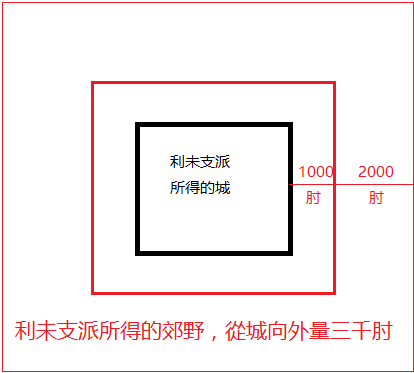
\includegraphics[width=.45\textwidth]{AMoXiFigs/minshuji/liwei}
\caption{利未支派得城的原則}
\end{center}
\end{figure} 
耶和華在摩押平原約旦河邊，耶利哥對面，曉諭摩西說：「你吩咐以色列人，要從所得為業的地中把些城給利未人居住，也要把這城四圍的郊野給利未人。這城邑要歸他們居住，城邑的郊野可以牧養他們的牛羊和各樣的牲畜，又可以安置他們的財物。你們給利未人的郊野，要從城根起，四圍往外量一千肘。另外東量二千肘、南量二千肘、西量二千肘、北量二千肘為邊界，城在當中。這要歸他們做城邑的郊野。你們給利未人的城邑，其中當有六座逃城，使誤殺人的可以逃到那裡，此外還要給他們四十二座城。你們要給利未人的城，共有四十八座，連城帶郊野都要給他們。以色列人所得的地業從中要把些城邑給利未人。人多的就多給，人少的就少給。各支派要按所承受為業之地把城邑給利未人。」


\subsubsection{設立逃城  35:9-15} 
耶和華曉諭摩西說：「你吩咐以色列人說：你們過約旦河，進了迦南地，就要分出幾座城，為你們做逃城，使誤殺人的可以逃到那裡。這些城可以做逃避報仇人的城，使誤殺人的不至於死，等他站在會眾面前聽審判。你們所分出來的城，要做六座逃城。在\textcolor{blue}{約旦河東}要分出三座城，在\textcolor{blue}{迦南地}也要分出三座城，都做逃城。這六座城要給\textcolor{blue}{以色列人}和他們\textcolor{blue}{中間的外人}，並\textcolor{blue}{寄居的}，作為逃城，使誤殺人的都可以逃到那裡。

\subsubsection{故殺人的逃城不能庇护 35:16-21} 
\begin{itemize} 
\itemsep-.35em
\item 若人\textcolor{blue}{用鐵器打人}，以致打死，他就是故殺人的，故殺人的必被治死。 
\item 若\textcolor{blue}{用可以打死人的石頭}打死了人，他就是故殺人的，故殺人的必被治死。 
\item 若\textcolor{blue}{用可以打死人的木器}打死了人，他就是故殺人的，故殺人的必被治死。報血仇的必親自殺那故殺人的，一遇見就殺他。 
\item 人若因\textcolor{blue}{怨恨把人推倒}，或是\textcolor{blue}{埋伏往人身上扔物}以至於死
\item 或是\textcolor{blue}{因仇恨用手打人}以至於死，那打人的必被治死。他是故殺人的，報血仇的一遇見就殺他。
\end{itemize}

\subsubsection{逃城的庇护原则  35:22-28} 
倘若人沒有仇恨，忽然將人推倒，或是沒有埋伏把物扔在人身上，或是沒有看見的時候用可以打死人的石頭扔在人身上，以至於死，本來與他無仇，也無意害他，會眾就要照典章，在打死人的和報血仇的中間審判。會眾要救這誤殺人的脫離報血仇人的手，也要使他歸入逃城。\\
他要住在其中，直等到受聖膏的大祭司死了。但誤殺人的，無論什麼時候，若出了逃城的境外，報血仇的在逃城境外遇見他，將他殺了，報血仇的就沒有流血之罪。 因為誤殺人的該住在逃城裡，等到大祭司死了。大祭司死了以後，誤殺人的才可以回到他所得為業之地。

\subsubsection{故殺人犯死罪的必被治死  35:29-34} 
「這在你們一切的住處，要做你們世世代代的律例、典章。無論誰故殺人，要憑幾個見證人的口把那故殺人的殺了，只是不可憑一個見證的口叫人死。故殺人，犯死罪的，你們\textcolor{red}{不可收贖價代替他的命}，他必被治死。那逃到逃城的人，你們不可為他收贖價，使他在大祭司未死以先再來住在本地。這樣，你們就不汙穢所住之地，因為血是汙穢地的。若有在地上流人血的，非流那殺人者的血，那地就不得潔淨(贖)。你們不可玷汙所住之地，就是我住在其中之地，因為我耶和華住在以色列人中間。」
 	
 	
\subsection{女子承地為業的條例 36 }
\subsubsection{瑪拿西族長在摩西和首領面前的诉求 36:1-4}
約瑟的後裔，瑪拿西的孫子、瑪吉的兒子基列，他子孫中的諸族長來到摩西和做首領的以色列人族長面前，說：「耶和華曾吩咐我主拈鬮分地給以色列人為業，我主也受了耶和華的吩咐將我們兄弟西羅非哈的產業分給他的眾女兒。她們若嫁以色列別支派的人，就必將我們祖宗所遺留的產業加在她們丈夫支派的產業中。這樣，我們拈鬮所得的產業就要減少了。到了以色列人的禧年，這女兒的產業就必加在她們丈夫支派的產業上。這樣，我們祖宗支派的產業就減少了。」
 
\subsubsection{得業女子必嫁同宗支派的人 36:5-9}
摩西照耶和華的話吩咐以色列人說：「約瑟支派的人說得有理。論到西羅非哈的眾女兒，耶和華這樣吩咐說：她們可以隨意嫁人，只是要嫁同宗支派的人。這樣，以色列人的產業就不從這支派歸到那支派，因為以色列人要各守各祖宗支派的產業。凡在以色列支派中得了產業的女子，必做同宗支派人的妻，好叫以色列人各自承受他祖宗的產業。這樣，他們的產業就不從這支派歸到那支派，因為以色列支派的人要各守各的產業。」

\subsubsection{西羅非哈的五女都嫁入瑪拿西子孫 36:10-12}
耶和華怎樣吩咐摩西，西羅非哈的眾女兒就怎樣行。西羅非哈的女兒瑪拉、得撒、曷拉、密迦、挪阿都嫁了她們伯叔的兒子。她們嫁入約瑟兒子瑪拿西子孫的族中，她們的產業仍留在同宗支派中。這是耶和華在摩押平原約旦河邊，耶利哥對面藉著摩西所吩咐以色列人的命令、典章。



\include{AMoXiFiles/ShenMingJi} 
\fi
\end{document}
